\documentclass[twoside]{book}

% Packages required by doxygen
\usepackage{calc}
\usepackage{doxygen}
\usepackage{graphicx}
\usepackage[utf8]{inputenc}
\usepackage{makeidx}
\usepackage{multicol}
\usepackage{multirow}
\usepackage{textcomp}
\usepackage[table]{xcolor}

% Font selection
\usepackage[T1]{fontenc}
\usepackage{mathptmx}
\usepackage[scaled=.90]{helvet}
\usepackage{courier}
\usepackage{amssymb}
\usepackage{sectsty}
\renewcommand{\familydefault}{\sfdefault}
\allsectionsfont{%
  \fontseries{bc}\selectfont%
  \color{darkgray}%
}
\renewcommand{\DoxyLabelFont}{%
  \fontseries{bc}\selectfont%
  \color{darkgray}%
}

% Page & text layout
\usepackage{geometry}
\geometry{%
  a4paper,%
  top=2.5cm,%
  bottom=2.5cm,%
  left=2.5cm,%
  right=2.5cm%
}
\tolerance=750
\hfuzz=15pt
\hbadness=750
\setlength{\emergencystretch}{15pt}
\setlength{\parindent}{0cm}
\setlength{\parskip}{0.2cm}
\makeatletter
\renewcommand{\paragraph}{%
  \@startsection{paragraph}{4}{0ex}{-1.0ex}{1.0ex}{%
    \normalfont\normalsize\bfseries\SS@parafont%
  }%
}
\renewcommand{\subparagraph}{%
  \@startsection{subparagraph}{5}{0ex}{-1.0ex}{1.0ex}{%
    \normalfont\normalsize\bfseries\SS@subparafont%
  }%
}
\makeatother

% Headers & footers
\usepackage{fancyhdr}
\pagestyle{fancyplain}
\fancyhead[LE]{\fancyplain{}{\bfseries\thepage}}
\fancyhead[CE]{\fancyplain{}{}}
\fancyhead[RE]{\fancyplain{}{\bfseries\leftmark}}
\fancyhead[LO]{\fancyplain{}{\bfseries\rightmark}}
\fancyhead[CO]{\fancyplain{}{}}
\fancyhead[RO]{\fancyplain{}{\bfseries\thepage}}
\fancyfoot[LE]{\fancyplain{}{}}
\fancyfoot[CE]{\fancyplain{}{}}
\fancyfoot[RE]{\fancyplain{}{\bfseries\scriptsize Generated on Tue Oct 7 2014 06\-:18\-:32 for Tanks A Lot by Doxygen }}
\fancyfoot[LO]{\fancyplain{}{\bfseries\scriptsize Generated on Tue Oct 7 2014 06\-:18\-:32 for Tanks A Lot by Doxygen }}
\fancyfoot[CO]{\fancyplain{}{}}
\fancyfoot[RO]{\fancyplain{}{}}
\renewcommand{\footrulewidth}{0.4pt}
\renewcommand{\chaptermark}[1]{%
  \markboth{#1}{}%
}
\renewcommand{\sectionmark}[1]{%
  \markright{\thesection\ #1}%
}

% Indices & bibliography
\usepackage{natbib}
\usepackage[titles]{tocloft}
\setcounter{tocdepth}{3}
\setcounter{secnumdepth}{5}
\makeindex

% Hyperlinks (required, but should be loaded last)
\usepackage{ifpdf}
\ifpdf
  \usepackage[pdftex,pagebackref=true]{hyperref}
\else
  \usepackage[ps2pdf,pagebackref=true]{hyperref}
\fi
\hypersetup{%
  colorlinks=true,%
  linkcolor=blue,%
  citecolor=blue,%
  unicode%
}

% Custom commands
\newcommand{\clearemptydoublepage}{%
  \newpage{\pagestyle{empty}\cleardoublepage}%
}


%===== C O N T E N T S =====

\begin{document}

% Titlepage & ToC
\hypersetup{pageanchor=false}
\pagenumbering{roman}
\begin{titlepage}
\vspace*{7cm}
\begin{center}%
{\Large Tanks A Lot }\\
\vspace*{1cm}
{\large Generated by Doxygen 1.8.6}\\
\vspace*{0.5cm}
{\small Tue Oct 7 2014 06:18:32}\\
\end{center}
\end{titlepage}
\clearemptydoublepage
\tableofcontents
\clearemptydoublepage
\pagenumbering{arabic}
\hypersetup{pageanchor=true}

%--- Begin generated contents ---
\chapter{\char`\"{}\-Tanks A Lot\char`\"{} Software Documentation}
\label{index}\hypertarget{index}{}Welcome! 
\chapter{Hierarchical Index}
\section{Class Hierarchy}
This inheritance list is sorted roughly, but not completely, alphabetically\-:\begin{DoxyCompactList}
\item \contentsline{section}{Action\-Data}{\pageref{classActionData}}{}
\begin{DoxyCompactList}
\item \contentsline{section}{Game\-Management\-Data}{\pageref{classGameManagementData}}{}
\end{DoxyCompactList}
\item \contentsline{section}{actions\-\_\-info}{\pageref{structactions__info}}{}
\item \contentsline{section}{coordinate}{\pageref{structcoordinate}}{}
\item \contentsline{section}{Deletable}{\pageref{classDeletable}}{}
\begin{DoxyCompactList}
\item \contentsline{section}{Collidable}{\pageref{classCollidable}}{}
\begin{DoxyCompactList}
\item \contentsline{section}{Barrier}{\pageref{classBarrier}}{}
\item \contentsline{section}{Mine}{\pageref{classMine}}{}
\item \contentsline{section}{Missile}{\pageref{classMissile}}{}
\item \contentsline{section}{Tank}{\pageref{classTank}}{}
\item \contentsline{section}{Turret}{\pageref{classTurret}}{}
\end{DoxyCompactList}
\item \contentsline{section}{Movable}{\pageref{classMovable}}{}
\begin{DoxyCompactList}
\item \contentsline{section}{Missile}{\pageref{classMissile}}{}
\item \contentsline{section}{Tank}{\pageref{classTank}}{}
\end{DoxyCompactList}
\item \contentsline{section}{Trackable}{\pageref{classTrackable}}{}
\begin{DoxyCompactList}
\item \contentsline{section}{Tank}{\pageref{classTank}}{}
\item \contentsline{section}{Turret}{\pageref{classTurret}}{}
\end{DoxyCompactList}
\end{DoxyCompactList}
\item \contentsline{section}{Display}{\pageref{classDisplay}}{}
\item \contentsline{section}{draw\-\_\-strings}{\pageref{structdraw__strings}}{}
\item \contentsline{section}{Game}{\pageref{classGame}}{}
\item \contentsline{section}{game\-\_\-state\-\_\-info}{\pageref{structgame__state__info}}{}
\item \contentsline{section}{Game\-State\-Data}{\pageref{classGameStateData}}{}
\begin{DoxyCompactList}
\item \contentsline{section}{Game\-Management\-Data}{\pageref{classGameManagementData}}{}
\end{DoxyCompactList}
\item \contentsline{section}{Geometry\-Engine}{\pageref{classGeometryEngine}}{}
\item \contentsline{section}{Invalid\-Constructor\-Arguments\-Barrier}{\pageref{classInvalidConstructorArgumentsBarrier}}{}
\item \contentsline{section}{Invalid\-Constructor\-Arguments\-Mine}{\pageref{classInvalidConstructorArgumentsMine}}{}
\item \contentsline{section}{Invalid\-Constructor\-Arguments\-Missile}{\pageref{classInvalidConstructorArgumentsMissile}}{}
\item \contentsline{section}{Invalid\-Constructor\-Arguments\-Tank}{\pageref{classInvalidConstructorArgumentsTank}}{}
\item \contentsline{section}{Invalid\-Constructor\-Arguments\-Turret}{\pageref{classInvalidConstructorArgumentsTurret}}{}
\item \contentsline{section}{Invalid\-Rect\-Entity\-Provided}{\pageref{classInvalidRectEntityProvided}}{}
\item \contentsline{section}{Invalid\-State\-Of\-Coordinates}{\pageref{classInvalidStateOfCoordinates}}{}
\item \contentsline{section}{Keyboard}{\pageref{classKeyboard}}{}
\item \contentsline{section}{Manager}{\pageref{classManager}}{}
\begin{DoxyCompactList}
\item \contentsline{section}{Collision\-Manager}{\pageref{classCollisionManager}}{}
\item \contentsline{section}{Destruction\-Manager}{\pageref{classDestructionManager}}{}
\item \contentsline{section}{Draw\-Manager}{\pageref{classDrawManager}}{}
\item \contentsline{section}{Game\-State\-Manager}{\pageref{classGameStateManager}}{}
\item \contentsline{section}{Move\-Manager}{\pageref{classMoveManager}}{}
\item \contentsline{section}{Tracking\-Manager}{\pageref{classTrackingManager}}{}
\item \contentsline{section}{Turret\-Manager}{\pageref{classTurretManager}}{}
\end{DoxyCompactList}
\item \contentsline{section}{Manager\-Test\-Assistant}{\pageref{classManagerTestAssistant}}{}
\item \contentsline{section}{Orientation}{\pageref{classOrientation}}{}
\item \contentsline{section}{rect\-\_\-corners}{\pageref{structrect__corners}}{}
\item \contentsline{section}{sprite\-\_\-draw\-\_\-info}{\pageref{structsprite__draw__info}}{}
\item \contentsline{section}{Sprite\-Dimensions}{\pageref{classSpriteDimensions}}{}
\item \contentsline{section}{Stop\-Watch}{\pageref{classStopWatch}}{}
\item \contentsline{section}{textures}{\pageref{structtextures}}{}
\end{DoxyCompactList}

\chapter{Class Index}
\section{Class List}
Here are the classes, structs, unions and interfaces with brief descriptions\-:\begin{DoxyCompactList}
\item\contentsline{section}{\hyperlink{classActionData}{Action\-Data} }{\pageref{classActionData}}{}
\item\contentsline{section}{\hyperlink{structactions__info}{actions\-\_\-info} \\*Player\-\_\-action is an enum of the possible actions that the tank can take }{\pageref{structactions__info}}{}
\item\contentsline{section}{\hyperlink{classBarrier}{Barrier} }{\pageref{classBarrier}}{}
\item\contentsline{section}{\hyperlink{classCollidable}{Collidable} }{\pageref{classCollidable}}{}
\item\contentsline{section}{\hyperlink{classCollisionManager}{Collision\-Manager} \\*\hyperlink{classManager}{Manager} class responsible for managing collisions }{\pageref{classCollisionManager}}{}
\item\contentsline{section}{\hyperlink{structcoordinate}{coordinate} \\*Basic Cartesian coordinate }{\pageref{structcoordinate}}{}
\item\contentsline{section}{\hyperlink{classDeletable}{Deletable} }{\pageref{classDeletable}}{}
\item\contentsline{section}{\hyperlink{classDestructionManager}{Destruction\-Manager} \\*\hyperlink{classManager}{Manager} class responsible for deletions of destroyed game entities }{\pageref{classDestructionManager}}{}
\item\contentsline{section}{\hyperlink{classDisplay}{Display} \\*Handles all draw and display functionality }{\pageref{classDisplay}}{}
\item\contentsline{section}{\hyperlink{structdraw__strings}{draw\-\_\-strings} \\*Holds the strings that will be drawn into text }{\pageref{structdraw__strings}}{}
\item\contentsline{section}{\hyperlink{classDrawManager}{Draw\-Manager} \\*\hyperlink{classManager}{Manager} class responsible for preparing draw data }{\pageref{classDrawManager}}{}
\item\contentsline{section}{\hyperlink{classGame}{Game} \\*Main class which runs the program loop }{\pageref{classGame}}{}
\item\contentsline{section}{\hyperlink{structgame__state__info}{game\-\_\-state\-\_\-info} \\*Contains information about the game state }{\pageref{structgame__state__info}}{}
\item\contentsline{section}{\hyperlink{classGameManagementData}{Game\-Management\-Data} \\*Implementation for the \hyperlink{classGameManagementData}{Game\-Management\-Data} Class }{\pageref{classGameManagementData}}{}
\item\contentsline{section}{\hyperlink{classGameStateData}{Game\-State\-Data} }{\pageref{classGameStateData}}{}
\item\contentsline{section}{\hyperlink{classGameStateManager}{Game\-State\-Manager} \\*\hyperlink{classManager}{Manager} class responsible for managing state of the game }{\pageref{classGameStateManager}}{}
\item\contentsline{section}{\hyperlink{classGeometryEngine}{Geometry\-Engine} \\*Class responisible for handling geometrical calculations }{\pageref{classGeometryEngine}}{}
\item\contentsline{section}{\hyperlink{classInvalidConstructorArgumentsBarrier}{Invalid\-Constructor\-Arguments\-Barrier} }{\pageref{classInvalidConstructorArgumentsBarrier}}{}
\item\contentsline{section}{\hyperlink{classInvalidConstructorArgumentsMine}{Invalid\-Constructor\-Arguments\-Mine} }{\pageref{classInvalidConstructorArgumentsMine}}{}
\item\contentsline{section}{\hyperlink{classInvalidConstructorArgumentsMissile}{Invalid\-Constructor\-Arguments\-Missile} }{\pageref{classInvalidConstructorArgumentsMissile}}{}
\item\contentsline{section}{\hyperlink{classInvalidConstructorArgumentsTank}{Invalid\-Constructor\-Arguments\-Tank} }{\pageref{classInvalidConstructorArgumentsTank}}{}
\item\contentsline{section}{\hyperlink{classInvalidConstructorArgumentsTurret}{Invalid\-Constructor\-Arguments\-Turret} }{\pageref{classInvalidConstructorArgumentsTurret}}{}
\item\contentsline{section}{\hyperlink{classInvalidRectEntityProvided}{Invalid\-Rect\-Entity\-Provided} }{\pageref{classInvalidRectEntityProvided}}{}
\item\contentsline{section}{\hyperlink{classInvalidStateOfCoordinates}{Invalid\-State\-Of\-Coordinates} }{\pageref{classInvalidStateOfCoordinates}}{}
\item\contentsline{section}{\hyperlink{classKeyboard}{Keyboard} \\*Simple class to act as an interface for S\-F\-M\-L keyboard functions }{\pageref{classKeyboard}}{}
\item\contentsline{section}{\hyperlink{classManager}{Manager} \\*Abstract-\/\-Base Class of Managers }{\pageref{classManager}}{}
\item\contentsline{section}{\hyperlink{classManagerTestAssistant}{Manager\-Test\-Assistant} }{\pageref{classManagerTestAssistant}}{}
\item\contentsline{section}{\hyperlink{classMine}{Mine} \\*Model class for a \hyperlink{classMine}{Mine} }{\pageref{classMine}}{}
\item\contentsline{section}{\hyperlink{classMissile}{Missile} \\*\hyperlink{classMissile}{Missile} Class implementation }{\pageref{classMissile}}{}
\item\contentsline{section}{\hyperlink{classMovable}{Movable} \\*An Abstract-\/based class forming an interface for all Moveable objects within the game }{\pageref{classMovable}}{}
\item\contentsline{section}{\hyperlink{classMoveManager}{Move\-Manager} }{\pageref{classMoveManager}}{}
\item\contentsline{section}{\hyperlink{classOrientation}{Orientation} }{\pageref{classOrientation}}{}
\item\contentsline{section}{\hyperlink{structrect__corners}{rect\-\_\-corners} \\*Contains x and y corners of a rectangle, used in the algorithm for collision detection }{\pageref{structrect__corners}}{}
\item\contentsline{section}{\hyperlink{structsprite__draw__info}{sprite\-\_\-draw\-\_\-info} \\*Used for passing information from draw manager to display }{\pageref{structsprite__draw__info}}{}
\item\contentsline{section}{\hyperlink{classSpriteDimensions}{Sprite\-Dimensions} }{\pageref{classSpriteDimensions}}{}
\item\contentsline{section}{\hyperlink{classStopWatch}{Stop\-Watch} \\*Responsible for keeping time }{\pageref{classStopWatch}}{}
\item\contentsline{section}{\hyperlink{classTank}{Tank} }{\pageref{classTank}}{}
\item\contentsline{section}{\hyperlink{structtextures}{textures} \\*All testures in the game }{\pageref{structtextures}}{}
\item\contentsline{section}{\hyperlink{classTrackable}{Trackable} \\*An Abstract-\/based class forming an interface for all \hyperlink{classTrackable}{Trackable} objects within the game }{\pageref{classTrackable}}{}
\item\contentsline{section}{\hyperlink{classTrackingManager}{Tracking\-Manager} \\*\hyperlink{classManager}{Manager} responsible for keeping track of game entity positions }{\pageref{classTrackingManager}}{}
\item\contentsline{section}{\hyperlink{classTurret}{Turret} }{\pageref{classTurret}}{}
\item\contentsline{section}{\hyperlink{classTurretManager}{Turret\-Manager} \\*\hyperlink{classManager}{Manager} responsible for controlling the turrets rotation }{\pageref{classTurretManager}}{}
\end{DoxyCompactList}

\chapter{File Index}
\section{File List}
Here is a list of all files with brief descriptions\-:\begin{DoxyCompactList}
\item\contentsline{section}{\hyperlink{ActionData_8h}{Action\-Data.\-h} \\*An Abstract-\/based class providing an interface for action data containing classes }{\pageref{ActionData_8h}}{}
\item\contentsline{section}{\hyperlink{Barrier_8cpp}{Barrier.\-cpp} \\*Implementation for the \hyperlink{classBarrier}{Barrier} Class }{\pageref{Barrier_8cpp}}{}
\item\contentsline{section}{\hyperlink{Barrier_8h}{Barrier.\-h} \\*A Composition-\/based class representing a simple barrier object within the game world }{\pageref{Barrier_8h}}{}
\item\contentsline{section}{\hyperlink{ClassTests_8cpp}{Class\-Tests.\-cpp} \\*Unit tests for all classes. Included in single file for regression testing purposes }{\pageref{ClassTests_8cpp}}{}
\item\contentsline{section}{\hyperlink{Collidable_8cpp}{Collidable.\-cpp} \\*Parent class for all objects capable of 'Colliding' within the game world }{\pageref{Collidable_8cpp}}{}
\item\contentsline{section}{\hyperlink{Collidable_8h}{Collidable.\-h} \\*An Abstract-\/based class forming an interface for all collidable model objects }{\pageref{Collidable_8h}}{}
\item\contentsline{section}{\hyperlink{CollisionManager_8cpp}{Collision\-Manager.\-cpp} \\*Implementation for \hyperlink{classCollisionManager}{Collision\-Manager} class }{\pageref{CollisionManager_8cpp}}{}
\item\contentsline{section}{\hyperlink{CollisionManager_8h}{Collision\-Manager.\-h} \\*\hyperlink{classManager}{Manager} class responsible for managing collisions }{\pageref{CollisionManager_8h}}{}
\item\contentsline{section}{\hyperlink{Deletable_8cpp}{Deletable.\-cpp} \\*Base class for all entities within the battle-\/tank world }{\pageref{Deletable_8cpp}}{}
\item\contentsline{section}{\hyperlink{Deletable_8h}{Deletable.\-h} \\*An Abstract-\/based class forming an interface for all deletable objects within the game }{\pageref{Deletable_8h}}{}
\item\contentsline{section}{\hyperlink{DestructionManager_8cpp}{Destruction\-Manager.\-cpp} \\*Implementation for the \hyperlink{classDestructionManager}{Destruction\-Manager} class }{\pageref{DestructionManager_8cpp}}{}
\item\contentsline{section}{\hyperlink{DestructionManager_8h}{Destruction\-Manager.\-h} \\*\hyperlink{classManager}{Manager} class responsible for deletions of destroyed game entities }{\pageref{DestructionManager_8h}}{}
\item\contentsline{section}{\hyperlink{Display_8cpp}{Display.\-cpp} \\*Implementation for \hyperlink{classDisplay}{Display} class }{\pageref{Display_8cpp}}{}
\item\contentsline{section}{\hyperlink{Display_8h}{Display.\-h} \\*Handles all draw and display functionality }{\pageref{Display_8h}}{}
\item\contentsline{section}{\hyperlink{DrawManager_8cpp}{Draw\-Manager.\-cpp} \\*Implementation for the \hyperlink{classDrawManager}{Draw\-Manager} class }{\pageref{DrawManager_8cpp}}{}
\item\contentsline{section}{\hyperlink{DrawManager_8h}{Draw\-Manager.\-h} \\*\hyperlink{classManager}{Manager} class responsible for preparing draw data }{\pageref{DrawManager_8h}}{}
\item\contentsline{section}{\hyperlink{Game_8cpp}{Game.\-cpp} \\*Implementation for \hyperlink{classGame}{Game} class }{\pageref{Game_8cpp}}{}
\item\contentsline{section}{\hyperlink{Game_8h}{Game.\-h} \\*Main class which runs the program loop }{\pageref{Game_8h}}{}
\item\contentsline{section}{\hyperlink{GameManagementData_8cpp}{Game\-Management\-Data.\-cpp} }{\pageref{GameManagementData_8cpp}}{}
\item\contentsline{section}{\hyperlink{GameManagementData_8h}{Game\-Management\-Data.\-h} \\*A data containter class which is passed to all managers }{\pageref{GameManagementData_8h}}{}
\item\contentsline{section}{\hyperlink{GameStateData_8h}{Game\-State\-Data.\-h} \\*An Abstract-\/based class providing an interface for game state data containing classes }{\pageref{GameStateData_8h}}{}
\item\contentsline{section}{\hyperlink{GameStateManager_8cpp}{Game\-State\-Manager.\-cpp} }{\pageref{GameStateManager_8cpp}}{}
\item\contentsline{section}{\hyperlink{GameStateManager_8h}{Game\-State\-Manager.\-h} }{\pageref{GameStateManager_8h}}{}
\item\contentsline{section}{\hyperlink{GeometryEngine_8cpp}{Geometry\-Engine.\-cpp} \\*Class responisible for handling geometrical calculations }{\pageref{GeometryEngine_8cpp}}{}
\item\contentsline{section}{\hyperlink{GeometryEngine_8h}{Geometry\-Engine.\-h} \\*Class responisible for handling geometrical calculations }{\pageref{GeometryEngine_8h}}{}
\item\contentsline{section}{\hyperlink{Keyboard_8cpp}{Keyboard.\-cpp} \\*Implementation for \hyperlink{classKeyboard}{Keyboard} class }{\pageref{Keyboard_8cpp}}{}
\item\contentsline{section}{\hyperlink{Keyboard_8h}{Keyboard.\-h} \\*Simple class to act as an interface for S\-F\-M\-L keyboard functions }{\pageref{Keyboard_8h}}{}
\item\contentsline{section}{\hyperlink{Manager_8cpp}{Manager.\-cpp} }{\pageref{Manager_8cpp}}{}
\item\contentsline{section}{\hyperlink{Manager_8h}{Manager.\-h} }{\pageref{Manager_8h}}{}
\item\contentsline{section}{\hyperlink{ManagerTestAssistant_8cpp}{Manager\-Test\-Assistant.\-cpp} \\*Class to assist in the correct running of Google Tests }{\pageref{ManagerTestAssistant_8cpp}}{}
\item\contentsline{section}{\hyperlink{ManagerTestAssistant_8h}{Manager\-Test\-Assistant.\-h} \\*Class to assist in the correct running of Google Tests }{\pageref{ManagerTestAssistant_8h}}{}
\item\contentsline{section}{\hyperlink{Mine_8cpp}{Mine.\-cpp} }{\pageref{Mine_8cpp}}{}
\item\contentsline{section}{\hyperlink{Mine_8h}{Mine.\-h} }{\pageref{Mine_8h}}{}
\item\contentsline{section}{\hyperlink{Missile_8cpp}{Missile.\-cpp} }{\pageref{Missile_8cpp}}{}
\item\contentsline{section}{\hyperlink{Missile_8h}{Missile.\-h} }{\pageref{Missile_8h}}{}
\item\contentsline{section}{\hyperlink{Movable_8cpp}{Movable.\-cpp} }{\pageref{Movable_8cpp}}{}
\item\contentsline{section}{\hyperlink{Movable_8h}{Movable.\-h} }{\pageref{Movable_8h}}{}
\item\contentsline{section}{\hyperlink{MoveManager_8cpp}{Move\-Manager.\-cpp} \\*\hyperlink{classManager}{Manager} responsible for moving all movable objects }{\pageref{MoveManager_8cpp}}{}
\item\contentsline{section}{\hyperlink{MoveManager_8h}{Move\-Manager.\-h} \\*\hyperlink{classManager}{Manager} responsible for moving all movable objects }{\pageref{MoveManager_8h}}{}
\item\contentsline{section}{\hyperlink{NewGame_8cpp}{New\-Game.\-cpp} \\*\hyperlink{classGame}{Game} class and the \hyperlink{classGame}{Game} is instansiated within this file }{\pageref{NewGame_8cpp}}{}
\item\contentsline{section}{\hyperlink{Orientation_8cpp}{Orientation.\-cpp} \\*Implementation for \hyperlink{classOrientation}{Orientation} class }{\pageref{Orientation_8cpp}}{}
\item\contentsline{section}{\hyperlink{Orientation_8h}{Orientation.\-h} \\*Class responsible for holding the ordinal data of all model entities within the game }{\pageref{Orientation_8h}}{}
\item\contentsline{section}{\hyperlink{SpriteDimensions_8cpp}{Sprite\-Dimensions.\-cpp} \\*A container class responsible for posssesing all the Sprite dimensions within the game world }{\pageref{SpriteDimensions_8cpp}}{}
\item\contentsline{section}{\hyperlink{SpriteDimensions_8h}{Sprite\-Dimensions.\-h} \\*A container class responsible for posssesing all the Sprite dimensions within the game world }{\pageref{SpriteDimensions_8h}}{}
\item\contentsline{section}{\hyperlink{StopWatch_8cpp}{Stop\-Watch.\-cpp} }{\pageref{StopWatch_8cpp}}{}
\item\contentsline{section}{\hyperlink{StopWatch_8h}{Stop\-Watch.\-h} \\*Implementation for time class }{\pageref{StopWatch_8h}}{}
\item\contentsline{section}{\hyperlink{Structures_8h}{Structures.\-h} \\*Keeps all structs in a single file }{\pageref{Structures_8h}}{}
\item\contentsline{section}{\hyperlink{Tank_8cpp}{Tank.\-cpp} \\*Implementation of the \hyperlink{classTank}{Tank} Class }{\pageref{Tank_8cpp}}{}
\item\contentsline{section}{\hyperlink{Tank_8h}{Tank.\-h} \\*Child class of \hyperlink{classMovable}{Movable}, \hyperlink{classCollidable}{Collidable}, \hyperlink{classTrackable}{Trackable}. The base \hyperlink{classTank}{Tank} entity }{\pageref{Tank_8h}}{}
\item\contentsline{section}{\hyperlink{TimingTest__BattleTanks_8cpp}{Timing\-Test\-\_\-\-Battle\-Tanks.\-cpp} }{\pageref{TimingTest__BattleTanks_8cpp}}{}
\item\contentsline{section}{\hyperlink{Trackable_8cpp}{Trackable.\-cpp} }{\pageref{Trackable_8cpp}}{}
\item\contentsline{section}{\hyperlink{Trackable_8h}{Trackable.\-h} \\*Parent class for all objects capable of being 'Tracked' within the game world }{\pageref{Trackable_8h}}{}
\item\contentsline{section}{\hyperlink{TrackingManager_8cpp}{Tracking\-Manager.\-cpp} }{\pageref{TrackingManager_8cpp}}{}
\item\contentsline{section}{\hyperlink{TrackingManager_8h}{Tracking\-Manager.\-h} \\*Model class for a \hyperlink{classMine}{Mine} }{\pageref{TrackingManager_8h}}{}
\item\contentsline{section}{\hyperlink{Turret_8cpp}{Turret.\-cpp} \\*Implementation of the \hyperlink{classTurret}{Turret} Class }{\pageref{Turret_8cpp}}{}
\item\contentsline{section}{\hyperlink{Turret_8h}{Turret.\-h} \\*Entity Class representing the \hyperlink{classTurret}{Turret} in the game world }{\pageref{Turret_8h}}{}
\item\contentsline{section}{\hyperlink{TurretManager_8cpp}{Turret\-Manager.\-cpp} \\*\hyperlink{classManager}{Manager} responsible for controlling the turrets rotation }{\pageref{TurretManager_8cpp}}{}
\item\contentsline{section}{\hyperlink{TurretManager_8h}{Turret\-Manager.\-h} \\*\hyperlink{classManager}{Manager} responsible for controlling the turrets rotation }{\pageref{TurretManager_8h}}{}
\end{DoxyCompactList}

\chapter{Class Documentation}
\hypertarget{classActionData}{\section{Action\-Data Class Reference}
\label{classActionData}\index{Action\-Data@{Action\-Data}}
}


{\ttfamily \#include $<$Action\-Data.\-h$>$}

Inheritance diagram for Action\-Data\-:\begin{figure}[H]
\begin{center}
\leavevmode
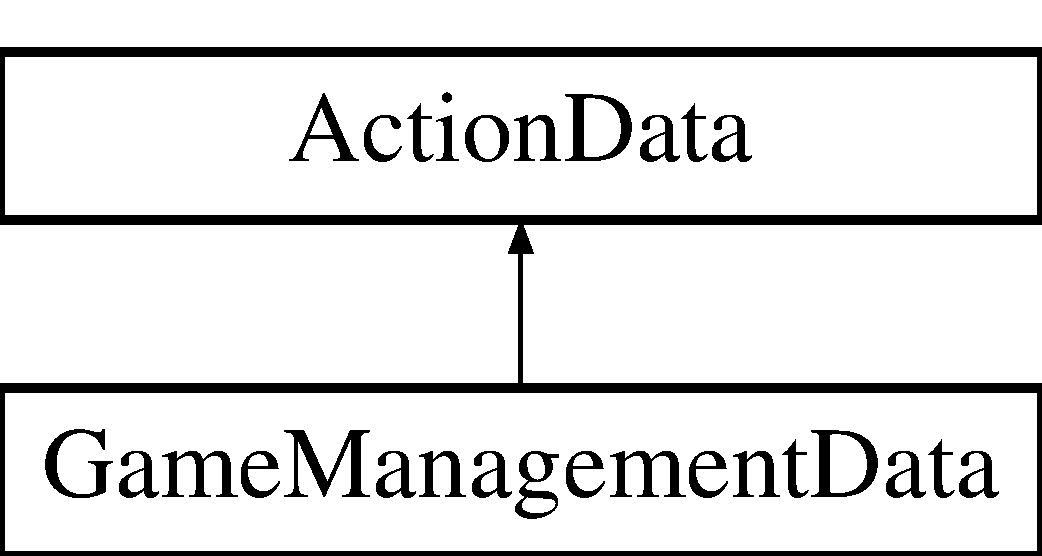
\includegraphics[height=2.000000cm]{classActionData}
\end{center}
\end{figure}
\subsection*{Public Member Functions}
\begin{DoxyCompactItemize}
\item 
virtual void \hyperlink{classActionData_aede7cfa65182cda2a2d43df11ccf2183}{reset\-Actions\-Info} ()=0
\begin{DoxyCompactList}\small\item\em Virtual void function, look to child for defenition. \end{DoxyCompactList}\item 
virtual const \hyperlink{structactions__info}{actions\-\_\-info} \& \hyperlink{classActionData_ab2f5b210968c91a01ed1439904b3ffee}{give\-Action\-Info} () const =0
\begin{DoxyCompactList}\small\item\em Provide the \hyperlink{structactions__info}{actions\-\_\-info} structure of a class. \end{DoxyCompactList}\item 
virtual void \hyperlink{classActionData_a043baaefa338dd8027ee3eec10f47e44}{reset\-Turret\-Fire} ()=0
\begin{DoxyCompactList}\small\item\em Virtual void function, look to child for defenition. \end{DoxyCompactList}\item 
virtual void \hyperlink{classActionData_a30502665240f4a0b0e37fbcd6447b590}{set\-Turret\-Fire} ()=0
\begin{DoxyCompactList}\small\item\em Virtual void function, look to child for defenition. \end{DoxyCompactList}\item 
virtual void \hyperlink{classActionData_a002859569085e9868adb7beabd3a2ad8}{move\-Forward\-P1} ()=0
\begin{DoxyCompactList}\small\item\em Virtual void function, look to child for defenition. \end{DoxyCompactList}\item 
virtual void \hyperlink{classActionData_a711265f479e845086896c42d1e906c57}{move\-Backward\-P1} ()=0
\begin{DoxyCompactList}\small\item\em Virtual void function, look to child for defenition. \end{DoxyCompactList}\item 
virtual void \hyperlink{classActionData_acca33ba2c7ea6df807d7e7b787733178}{rotate\-Left\-P1} ()=0
\begin{DoxyCompactList}\small\item\em Virtual void function, look to child for defenition. \end{DoxyCompactList}\item 
virtual void \hyperlink{classActionData_af780bdc2145493cb28b7f9dbee238328}{rotate\-Right\-P1} ()=0
\begin{DoxyCompactList}\small\item\em Virtual void function, look to child for defenition. \end{DoxyCompactList}\item 
virtual void \hyperlink{classActionData_a30c547419564c80e3764b620bb1833cc}{move\-Forward\-P2} ()=0
\begin{DoxyCompactList}\small\item\em Virtual void function, look to child for defenition. \end{DoxyCompactList}\item 
virtual void \hyperlink{classActionData_a9914514aed490cdf131f4a4be4d0f411}{move\-Backward\-P2} ()=0
\begin{DoxyCompactList}\small\item\em Virtual void function, look to child for defenition. \end{DoxyCompactList}\item 
virtual void \hyperlink{classActionData_aa67078569c7aa6f0f39449c2e9d20abf}{rotate\-Left\-P2} ()=0
\begin{DoxyCompactList}\small\item\em Virtual void function, look to child for defenition. \end{DoxyCompactList}\item 
virtual void \hyperlink{classActionData_aae9de974e0b844d04eec06087d867246}{rotate\-Right\-P2} ()=0
\begin{DoxyCompactList}\small\item\em Virtual void function, look to child for defenition. \end{DoxyCompactList}\item 
virtual void \hyperlink{classActionData_aeb7f1219ff0bf0cc81fee1d669317cdb}{missile\-Fired\-P1} ()=0
\begin{DoxyCompactList}\small\item\em Virtual void function, look to child for defenition. \end{DoxyCompactList}\item 
virtual void \hyperlink{classActionData_a5a2d45d0fc03daf8edaacd6a9757fafd}{missile\-Fired\-P2} ()=0
\begin{DoxyCompactList}\small\item\em Virtual void function, look to child for defenition. \end{DoxyCompactList}\item 
virtual void \hyperlink{classActionData_a8abc4e84c4e6d676010c7e2497278312}{mine\-Laid\-P1} ()=0
\begin{DoxyCompactList}\small\item\em Virtual void function, look to child for defenition. \end{DoxyCompactList}\item 
virtual void \hyperlink{classActionData_a71c04f577d3c06aa45b7c43d935ca567}{mine\-Laid\-P2} ()=0
\begin{DoxyCompactList}\small\item\em Virtual void function, look to child for defenition. \end{DoxyCompactList}\item 
virtual void \hyperlink{classActionData_a12925d051a1cd40bddcb18f0be2c2b01}{reset\-P1\-Attack} ()=0
\begin{DoxyCompactList}\small\item\em Virtual void function, look to child for defenition. \end{DoxyCompactList}\item 
virtual void \hyperlink{classActionData_ab8a96447019bfc7a275903dfa42cfcf5}{reset\-P2\-Attack} ()=0
\begin{DoxyCompactList}\small\item\em Virtual void function, look to child for defenition. \end{DoxyCompactList}\item 
virtual \hyperlink{classActionData_ad26f0ce70e0e397572dce0c87af1665a}{$\sim$\-Action\-Data} ()
\begin{DoxyCompactList}\small\item\em Destructor for Action Data. \end{DoxyCompactList}\end{DoxyCompactItemize}


\subsection{Detailed Description}


Definition at line 16 of file Action\-Data.\-h.



\subsection{Constructor \& Destructor Documentation}
\hypertarget{classActionData_ad26f0ce70e0e397572dce0c87af1665a}{\index{Action\-Data@{Action\-Data}!$\sim$\-Action\-Data@{$\sim$\-Action\-Data}}
\index{$\sim$\-Action\-Data@{$\sim$\-Action\-Data}!ActionData@{Action\-Data}}
\subsubsection[{$\sim$\-Action\-Data}]{\setlength{\rightskip}{0pt plus 5cm}virtual Action\-Data\-::$\sim$\-Action\-Data (
\begin{DoxyParamCaption}
{}
\end{DoxyParamCaption}
)\hspace{0.3cm}{\ttfamily [inline]}, {\ttfamily [virtual]}}}\label{classActionData_ad26f0ce70e0e397572dce0c87af1665a}


Destructor for Action Data. 



Definition at line 57 of file Action\-Data.\-h.


\begin{DoxyCode}
57 \{\};
\end{DoxyCode}


\subsection{Member Function Documentation}
\hypertarget{classActionData_ab2f5b210968c91a01ed1439904b3ffee}{\index{Action\-Data@{Action\-Data}!give\-Action\-Info@{give\-Action\-Info}}
\index{give\-Action\-Info@{give\-Action\-Info}!ActionData@{Action\-Data}}
\subsubsection[{give\-Action\-Info}]{\setlength{\rightskip}{0pt plus 5cm}virtual const {\bf actions\-\_\-info}\& Action\-Data\-::give\-Action\-Info (
\begin{DoxyParamCaption}
{}
\end{DoxyParamCaption}
) const\hspace{0.3cm}{\ttfamily [pure virtual]}}}\label{classActionData_ab2f5b210968c91a01ed1439904b3ffee}


Provide the \hyperlink{structactions__info}{actions\-\_\-info} structure of a class. 



Implemented in \hyperlink{classGameManagementData_afa213f0d90a9d0878fae317457f5e851}{Game\-Management\-Data}.



Referenced by Move\-Manager\-::manage(), and Game\-State\-Manager\-::manage\-Attack\-Timers().

\hypertarget{classActionData_a8abc4e84c4e6d676010c7e2497278312}{\index{Action\-Data@{Action\-Data}!mine\-Laid\-P1@{mine\-Laid\-P1}}
\index{mine\-Laid\-P1@{mine\-Laid\-P1}!ActionData@{Action\-Data}}
\subsubsection[{mine\-Laid\-P1}]{\setlength{\rightskip}{0pt plus 5cm}virtual void Action\-Data\-::mine\-Laid\-P1 (
\begin{DoxyParamCaption}
{}
\end{DoxyParamCaption}
)\hspace{0.3cm}{\ttfamily [pure virtual]}}}\label{classActionData_a8abc4e84c4e6d676010c7e2497278312}


Virtual void function, look to child for defenition. 



Implemented in \hyperlink{classGameManagementData_a5450f20ab4ad8d8f81c4d673ea72bfc2}{Game\-Management\-Data}.



Referenced by Game\-::check\-Keyboard\-Input().

\hypertarget{classActionData_a71c04f577d3c06aa45b7c43d935ca567}{\index{Action\-Data@{Action\-Data}!mine\-Laid\-P2@{mine\-Laid\-P2}}
\index{mine\-Laid\-P2@{mine\-Laid\-P2}!ActionData@{Action\-Data}}
\subsubsection[{mine\-Laid\-P2}]{\setlength{\rightskip}{0pt plus 5cm}virtual void Action\-Data\-::mine\-Laid\-P2 (
\begin{DoxyParamCaption}
{}
\end{DoxyParamCaption}
)\hspace{0.3cm}{\ttfamily [pure virtual]}}}\label{classActionData_a71c04f577d3c06aa45b7c43d935ca567}


Virtual void function, look to child for defenition. 



Implemented in \hyperlink{classGameManagementData_a794b882a00b5c979e59590db0c452828}{Game\-Management\-Data}.



Referenced by Game\-::check\-Keyboard\-Input().

\hypertarget{classActionData_aeb7f1219ff0bf0cc81fee1d669317cdb}{\index{Action\-Data@{Action\-Data}!missile\-Fired\-P1@{missile\-Fired\-P1}}
\index{missile\-Fired\-P1@{missile\-Fired\-P1}!ActionData@{Action\-Data}}
\subsubsection[{missile\-Fired\-P1}]{\setlength{\rightskip}{0pt plus 5cm}virtual void Action\-Data\-::missile\-Fired\-P1 (
\begin{DoxyParamCaption}
{}
\end{DoxyParamCaption}
)\hspace{0.3cm}{\ttfamily [pure virtual]}}}\label{classActionData_aeb7f1219ff0bf0cc81fee1d669317cdb}


Virtual void function, look to child for defenition. 



Implemented in \hyperlink{classGameManagementData_af31200e3fa7302496f48d81ad3934ace}{Game\-Management\-Data}.



Referenced by Game\-::check\-Keyboard\-Input().

\hypertarget{classActionData_a5a2d45d0fc03daf8edaacd6a9757fafd}{\index{Action\-Data@{Action\-Data}!missile\-Fired\-P2@{missile\-Fired\-P2}}
\index{missile\-Fired\-P2@{missile\-Fired\-P2}!ActionData@{Action\-Data}}
\subsubsection[{missile\-Fired\-P2}]{\setlength{\rightskip}{0pt plus 5cm}virtual void Action\-Data\-::missile\-Fired\-P2 (
\begin{DoxyParamCaption}
{}
\end{DoxyParamCaption}
)\hspace{0.3cm}{\ttfamily [pure virtual]}}}\label{classActionData_a5a2d45d0fc03daf8edaacd6a9757fafd}


Virtual void function, look to child for defenition. 



Implemented in \hyperlink{classGameManagementData_ae55ccfb644fc58de62c42779dbf710c4}{Game\-Management\-Data}.



Referenced by Game\-::check\-Keyboard\-Input().

\hypertarget{classActionData_a711265f479e845086896c42d1e906c57}{\index{Action\-Data@{Action\-Data}!move\-Backward\-P1@{move\-Backward\-P1}}
\index{move\-Backward\-P1@{move\-Backward\-P1}!ActionData@{Action\-Data}}
\subsubsection[{move\-Backward\-P1}]{\setlength{\rightskip}{0pt plus 5cm}virtual void Action\-Data\-::move\-Backward\-P1 (
\begin{DoxyParamCaption}
{}
\end{DoxyParamCaption}
)\hspace{0.3cm}{\ttfamily [pure virtual]}}}\label{classActionData_a711265f479e845086896c42d1e906c57}


Virtual void function, look to child for defenition. 



Implemented in \hyperlink{classGameManagementData_ab023b818d0ffc740fc5574654ff89cfa}{Game\-Management\-Data}.



Referenced by Game\-::check\-Keyboard\-Input().

\hypertarget{classActionData_a9914514aed490cdf131f4a4be4d0f411}{\index{Action\-Data@{Action\-Data}!move\-Backward\-P2@{move\-Backward\-P2}}
\index{move\-Backward\-P2@{move\-Backward\-P2}!ActionData@{Action\-Data}}
\subsubsection[{move\-Backward\-P2}]{\setlength{\rightskip}{0pt plus 5cm}virtual void Action\-Data\-::move\-Backward\-P2 (
\begin{DoxyParamCaption}
{}
\end{DoxyParamCaption}
)\hspace{0.3cm}{\ttfamily [pure virtual]}}}\label{classActionData_a9914514aed490cdf131f4a4be4d0f411}


Virtual void function, look to child for defenition. 



Implemented in \hyperlink{classGameManagementData_a130c7b68c41bfcc92bae027f5db11e68}{Game\-Management\-Data}.



Referenced by Game\-::check\-Keyboard\-Input().

\hypertarget{classActionData_a002859569085e9868adb7beabd3a2ad8}{\index{Action\-Data@{Action\-Data}!move\-Forward\-P1@{move\-Forward\-P1}}
\index{move\-Forward\-P1@{move\-Forward\-P1}!ActionData@{Action\-Data}}
\subsubsection[{move\-Forward\-P1}]{\setlength{\rightskip}{0pt plus 5cm}virtual void Action\-Data\-::move\-Forward\-P1 (
\begin{DoxyParamCaption}
{}
\end{DoxyParamCaption}
)\hspace{0.3cm}{\ttfamily [pure virtual]}}}\label{classActionData_a002859569085e9868adb7beabd3a2ad8}


Virtual void function, look to child for defenition. 



Implemented in \hyperlink{classGameManagementData_a4ad4fccb78261b8299142db3185828e3}{Game\-Management\-Data}.



Referenced by Game\-::check\-Keyboard\-Input().

\hypertarget{classActionData_a30c547419564c80e3764b620bb1833cc}{\index{Action\-Data@{Action\-Data}!move\-Forward\-P2@{move\-Forward\-P2}}
\index{move\-Forward\-P2@{move\-Forward\-P2}!ActionData@{Action\-Data}}
\subsubsection[{move\-Forward\-P2}]{\setlength{\rightskip}{0pt plus 5cm}virtual void Action\-Data\-::move\-Forward\-P2 (
\begin{DoxyParamCaption}
{}
\end{DoxyParamCaption}
)\hspace{0.3cm}{\ttfamily [pure virtual]}}}\label{classActionData_a30c547419564c80e3764b620bb1833cc}


Virtual void function, look to child for defenition. 



Implemented in \hyperlink{classGameManagementData_ab434e39574c0511a37bd5799607dc782}{Game\-Management\-Data}.



Referenced by Game\-::check\-Keyboard\-Input().

\hypertarget{classActionData_aede7cfa65182cda2a2d43df11ccf2183}{\index{Action\-Data@{Action\-Data}!reset\-Actions\-Info@{reset\-Actions\-Info}}
\index{reset\-Actions\-Info@{reset\-Actions\-Info}!ActionData@{Action\-Data}}
\subsubsection[{reset\-Actions\-Info}]{\setlength{\rightskip}{0pt plus 5cm}virtual void Action\-Data\-::reset\-Actions\-Info (
\begin{DoxyParamCaption}
{}
\end{DoxyParamCaption}
)\hspace{0.3cm}{\ttfamily [pure virtual]}}}\label{classActionData_aede7cfa65182cda2a2d43df11ccf2183}


Virtual void function, look to child for defenition. 



Implemented in \hyperlink{classGameManagementData_ae49afd739e313caf0b5cd3799be1b125}{Game\-Management\-Data}.

\hypertarget{classActionData_a12925d051a1cd40bddcb18f0be2c2b01}{\index{Action\-Data@{Action\-Data}!reset\-P1\-Attack@{reset\-P1\-Attack}}
\index{reset\-P1\-Attack@{reset\-P1\-Attack}!ActionData@{Action\-Data}}
\subsubsection[{reset\-P1\-Attack}]{\setlength{\rightskip}{0pt plus 5cm}virtual void Action\-Data\-::reset\-P1\-Attack (
\begin{DoxyParamCaption}
{}
\end{DoxyParamCaption}
)\hspace{0.3cm}{\ttfamily [pure virtual]}}}\label{classActionData_a12925d051a1cd40bddcb18f0be2c2b01}


Virtual void function, look to child for defenition. 



Implemented in \hyperlink{classGameManagementData_a82c3d16a50fb6e79a3b9aaca2272d000}{Game\-Management\-Data}.



Referenced by Game\-State\-Manager\-::manage\-Attack\-Timers().

\hypertarget{classActionData_ab8a96447019bfc7a275903dfa42cfcf5}{\index{Action\-Data@{Action\-Data}!reset\-P2\-Attack@{reset\-P2\-Attack}}
\index{reset\-P2\-Attack@{reset\-P2\-Attack}!ActionData@{Action\-Data}}
\subsubsection[{reset\-P2\-Attack}]{\setlength{\rightskip}{0pt plus 5cm}virtual void Action\-Data\-::reset\-P2\-Attack (
\begin{DoxyParamCaption}
{}
\end{DoxyParamCaption}
)\hspace{0.3cm}{\ttfamily [pure virtual]}}}\label{classActionData_ab8a96447019bfc7a275903dfa42cfcf5}


Virtual void function, look to child for defenition. 



Implemented in \hyperlink{classGameManagementData_a3434062fcb5872de24787b2cfa49b605}{Game\-Management\-Data}.



Referenced by Game\-State\-Manager\-::manage\-Attack\-Timers().

\hypertarget{classActionData_a043baaefa338dd8027ee3eec10f47e44}{\index{Action\-Data@{Action\-Data}!reset\-Turret\-Fire@{reset\-Turret\-Fire}}
\index{reset\-Turret\-Fire@{reset\-Turret\-Fire}!ActionData@{Action\-Data}}
\subsubsection[{reset\-Turret\-Fire}]{\setlength{\rightskip}{0pt plus 5cm}virtual void Action\-Data\-::reset\-Turret\-Fire (
\begin{DoxyParamCaption}
{}
\end{DoxyParamCaption}
)\hspace{0.3cm}{\ttfamily [pure virtual]}}}\label{classActionData_a043baaefa338dd8027ee3eec10f47e44}


Virtual void function, look to child for defenition. 



Implemented in \hyperlink{classGameManagementData_a2e9acf1ddddabee775dc106b478aa2e2}{Game\-Management\-Data}.

\hypertarget{classActionData_acca33ba2c7ea6df807d7e7b787733178}{\index{Action\-Data@{Action\-Data}!rotate\-Left\-P1@{rotate\-Left\-P1}}
\index{rotate\-Left\-P1@{rotate\-Left\-P1}!ActionData@{Action\-Data}}
\subsubsection[{rotate\-Left\-P1}]{\setlength{\rightskip}{0pt plus 5cm}virtual void Action\-Data\-::rotate\-Left\-P1 (
\begin{DoxyParamCaption}
{}
\end{DoxyParamCaption}
)\hspace{0.3cm}{\ttfamily [pure virtual]}}}\label{classActionData_acca33ba2c7ea6df807d7e7b787733178}


Virtual void function, look to child for defenition. 



Implemented in \hyperlink{classGameManagementData_afe92b173c32488f148fc7a2fa3ac0388}{Game\-Management\-Data}.



Referenced by Game\-::check\-Keyboard\-Input().

\hypertarget{classActionData_aa67078569c7aa6f0f39449c2e9d20abf}{\index{Action\-Data@{Action\-Data}!rotate\-Left\-P2@{rotate\-Left\-P2}}
\index{rotate\-Left\-P2@{rotate\-Left\-P2}!ActionData@{Action\-Data}}
\subsubsection[{rotate\-Left\-P2}]{\setlength{\rightskip}{0pt plus 5cm}virtual void Action\-Data\-::rotate\-Left\-P2 (
\begin{DoxyParamCaption}
{}
\end{DoxyParamCaption}
)\hspace{0.3cm}{\ttfamily [pure virtual]}}}\label{classActionData_aa67078569c7aa6f0f39449c2e9d20abf}


Virtual void function, look to child for defenition. 



Implemented in \hyperlink{classGameManagementData_a7b6ba982e678159bd687243facce3ab2}{Game\-Management\-Data}.



Referenced by Game\-::check\-Keyboard\-Input().

\hypertarget{classActionData_af780bdc2145493cb28b7f9dbee238328}{\index{Action\-Data@{Action\-Data}!rotate\-Right\-P1@{rotate\-Right\-P1}}
\index{rotate\-Right\-P1@{rotate\-Right\-P1}!ActionData@{Action\-Data}}
\subsubsection[{rotate\-Right\-P1}]{\setlength{\rightskip}{0pt plus 5cm}virtual void Action\-Data\-::rotate\-Right\-P1 (
\begin{DoxyParamCaption}
{}
\end{DoxyParamCaption}
)\hspace{0.3cm}{\ttfamily [pure virtual]}}}\label{classActionData_af780bdc2145493cb28b7f9dbee238328}


Virtual void function, look to child for defenition. 



Implemented in \hyperlink{classGameManagementData_a933b945bef3e7b15306ed361f611ec2d}{Game\-Management\-Data}.



Referenced by Game\-::check\-Keyboard\-Input().

\hypertarget{classActionData_aae9de974e0b844d04eec06087d867246}{\index{Action\-Data@{Action\-Data}!rotate\-Right\-P2@{rotate\-Right\-P2}}
\index{rotate\-Right\-P2@{rotate\-Right\-P2}!ActionData@{Action\-Data}}
\subsubsection[{rotate\-Right\-P2}]{\setlength{\rightskip}{0pt plus 5cm}virtual void Action\-Data\-::rotate\-Right\-P2 (
\begin{DoxyParamCaption}
{}
\end{DoxyParamCaption}
)\hspace{0.3cm}{\ttfamily [pure virtual]}}}\label{classActionData_aae9de974e0b844d04eec06087d867246}


Virtual void function, look to child for defenition. 



Implemented in \hyperlink{classGameManagementData_a93b5d21e2b4e347e8d7051885aab2bb2}{Game\-Management\-Data}.



Referenced by Game\-::check\-Keyboard\-Input().

\hypertarget{classActionData_a30502665240f4a0b0e37fbcd6447b590}{\index{Action\-Data@{Action\-Data}!set\-Turret\-Fire@{set\-Turret\-Fire}}
\index{set\-Turret\-Fire@{set\-Turret\-Fire}!ActionData@{Action\-Data}}
\subsubsection[{set\-Turret\-Fire}]{\setlength{\rightskip}{0pt plus 5cm}virtual void Action\-Data\-::set\-Turret\-Fire (
\begin{DoxyParamCaption}
{}
\end{DoxyParamCaption}
)\hspace{0.3cm}{\ttfamily [pure virtual]}}}\label{classActionData_a30502665240f4a0b0e37fbcd6447b590}


Virtual void function, look to child for defenition. 



Implemented in \hyperlink{classGameManagementData_aa3e5f9aaa99a44c4518933ad75b7ccd6}{Game\-Management\-Data}.



Referenced by Tracking\-Manager\-::manage().



The documentation for this class was generated from the following file\-:\begin{DoxyCompactItemize}
\item 
\hyperlink{ActionData_8h}{Action\-Data.\-h}\end{DoxyCompactItemize}

\hypertarget{structactions__info}{\section{actions\+\_\+info Struct Reference}
\label{structactions__info}\index{actions\+\_\+info@{actions\+\_\+info}}
}


player\+\_\+action is an enum of the possible actions that the tank can take  




{\ttfamily \#include $<$Structures.\+h$>$}

\subsection*{Public Attributes}
\begin{DoxyCompactItemize}
\item 
\hypertarget{structactions__info_a69ac673533838f973f09492a12516816}{bool {\bfseries change\+\_\+1}}\label{structactions__info_a69ac673533838f973f09492a12516816}

\item 
\hypertarget{structactions__info_a0f20d9c244d92a71dad9cf8ce10cd2f2}{bool {\bfseries change\+\_\+2}}\label{structactions__info_a0f20d9c244d92a71dad9cf8ce10cd2f2}

\item 
\hypertarget{structactions__info_afd5886948959786f75255fccbc965154}{bool {\bfseries turret\+\_\+fire}}\label{structactions__info_afd5886948959786f75255fccbc965154}

\item 
\hypertarget{structactions__info_a5cb853144009b2bfb7e58c7bf43e2a42}{player\+\_\+action {\bfseries move\+\_\+1}}\label{structactions__info_a5cb853144009b2bfb7e58c7bf43e2a42}

\item 
\hypertarget{structactions__info_adf9ed4a9ad4b604295846d06872e0ebf}{player\+\_\+action {\bfseries move\+\_\+2}}\label{structactions__info_adf9ed4a9ad4b604295846d06872e0ebf}

\item 
\hypertarget{structactions__info_a722a3805cc06ba6e5f9627b942f9bbf2}{player\+\_\+action {\bfseries attack\+\_\+1}}\label{structactions__info_a722a3805cc06ba6e5f9627b942f9bbf2}

\item 
\hypertarget{structactions__info_a9bfb93ce33b8969b45fa72a12b89be89}{player\+\_\+action {\bfseries attack\+\_\+2}}\label{structactions__info_a9bfb93ce33b8969b45fa72a12b89be89}

\end{DoxyCompactItemize}


\subsection{Detailed Description}
player\+\_\+action is an enum of the possible actions that the tank can take 

Definition at line 56 of file Structures.\+h.



The documentation for this struct was generated from the following file\+:\begin{DoxyCompactItemize}
\item 
\hyperlink{_structures_8h}{Structures.\+h}\end{DoxyCompactItemize}

\hypertarget{classBarrier}{\section{Barrier Class Reference}
\label{classBarrier}\index{Barrier@{Barrier}}
}


{\ttfamily \#include $<$Barrier.\-h$>$}

Inheritance diagram for Barrier\-:\begin{figure}[H]
\begin{center}
\leavevmode
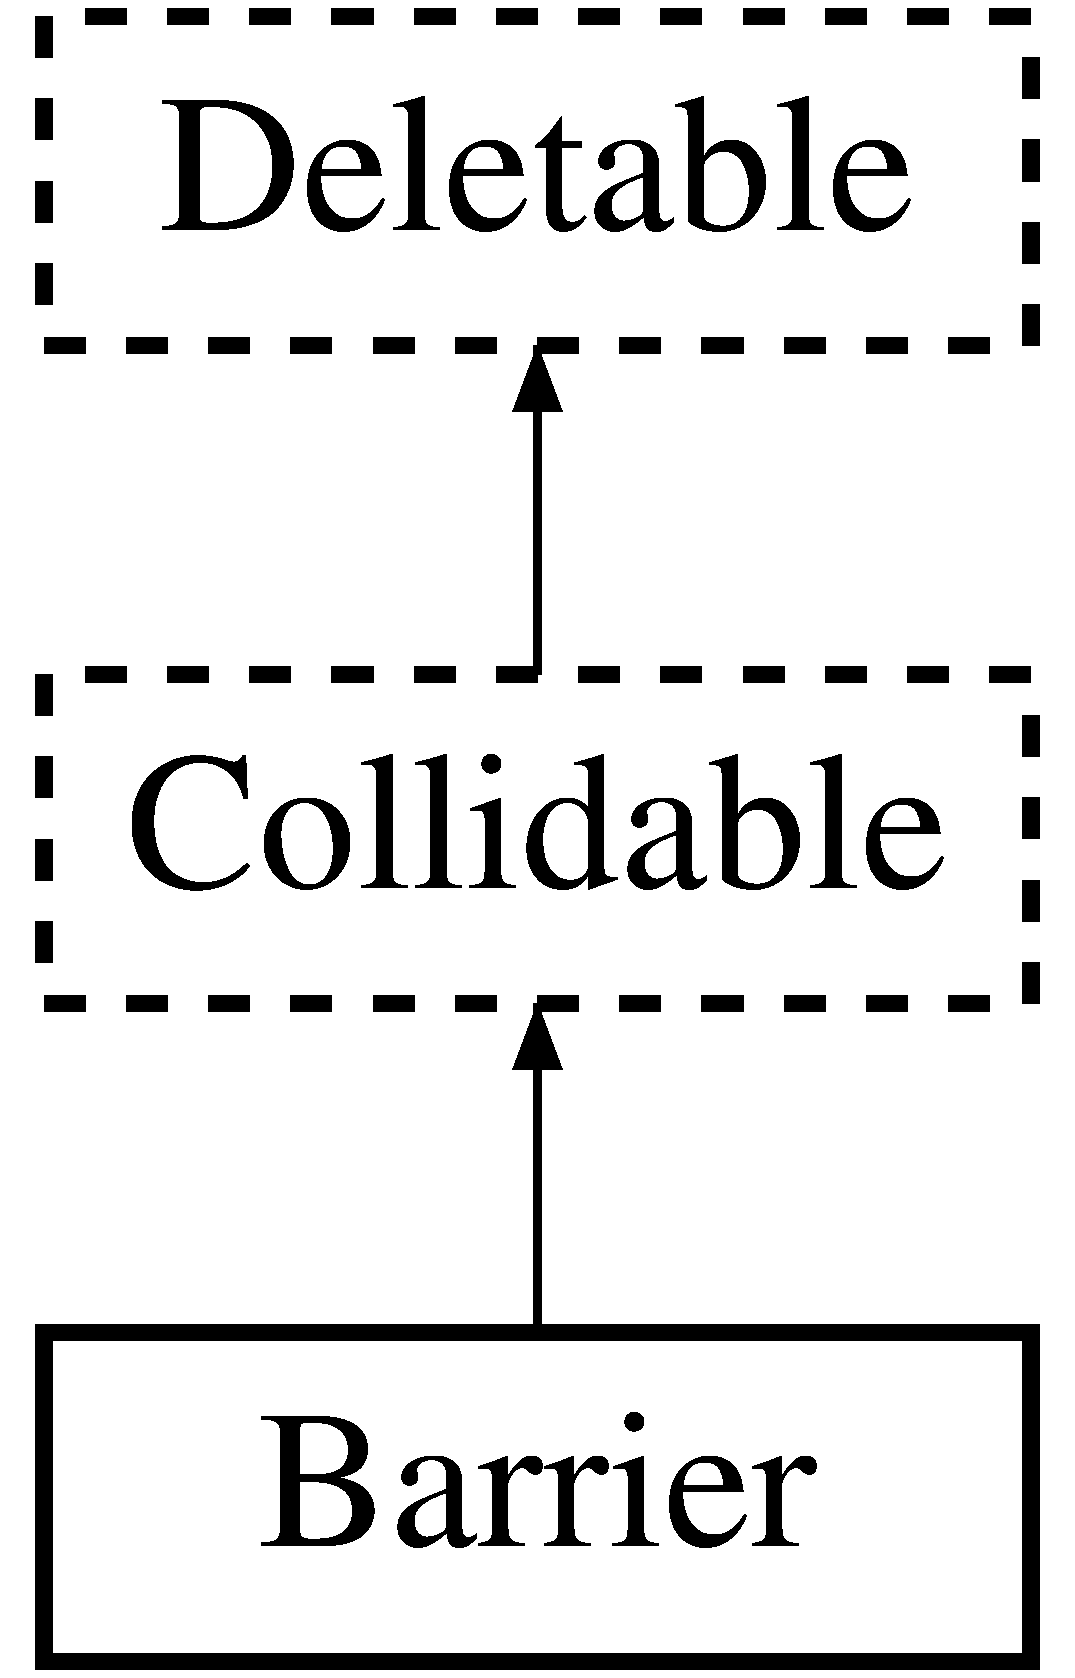
\includegraphics[height=3.000000cm]{classBarrier}
\end{center}
\end{figure}
\subsection*{Public Member Functions}
\begin{DoxyCompactItemize}
\item 
\hyperlink{classBarrier_aa5930a2e2b7cfc516a9badd3fcc8babd}{Barrier} (float position\-X, float position\-Y, \hyperlink{Structures_8h_a6d8f83e710b27d4f86c45f0bb77066e3}{entity\-\_\-type} barrier\-Type\-Set)
\begin{DoxyCompactList}\small\item\em \hyperlink{classBarrier}{Barrier} entity constructor. \end{DoxyCompactList}\item 
virtual const \hyperlink{Structures_8h_a6d8f83e710b27d4f86c45f0bb77066e3}{entity\-\_\-type} \& \hyperlink{classBarrier_a649b80eadc6948e68947f7516fee258c}{get\-Type} () const 
\begin{DoxyCompactList}\small\item\em \hyperlink{classBarrier}{Barrier} is able to provide its identification. \end{DoxyCompactList}\item 
virtual const \hyperlink{structrect__corners}{rect\-\_\-corners} \& \hyperlink{classBarrier_a050de6c9ffbb0a321c6d8a2e3d1dd418}{get\-Bounding\-Box} ()
\begin{DoxyCompactList}\small\item\em Provide the bounding box for the \hyperlink{classBarrier}{Barrier} entity. \end{DoxyCompactList}\item 
virtual const \hyperlink{structrect__corners}{rect\-\_\-corners} \& \hyperlink{classBarrier_a5fe813c8e78457566a5ff61235c12ea6}{get\-Aligned\-Bounding\-Box} ()
\begin{DoxyCompactList}\small\item\em Get Axis Aligned bounding box of entity. \end{DoxyCompactList}\item 
virtual const int \hyperlink{classBarrier_acff61ab4742c427abdf0d46abd52c832}{set\-Blocked} (const \hyperlink{Structures_8h_a6fef29d9424addfa69bdd2a379424896}{blocked\-\_\-status} obstruction\-\_\-type)
\begin{DoxyCompactList}\small\item\em This function is not used by barrier. \end{DoxyCompactList}\item 
virtual void \hyperlink{classBarrier_a863ef65ef677abdcf97373157f86c138}{set\-Unblocked} ()
\begin{DoxyCompactList}\small\item\em This function is not used by barrier. \end{DoxyCompactList}\item 
virtual void \hyperlink{classBarrier_adeedae22d7df279613359026ecf9f279}{set\-Collided} ()
\begin{DoxyCompactList}\small\item\em This function may be implmented later$\ast$$\ast$. \end{DoxyCompactList}\item 
virtual const bool \hyperlink{classBarrier_a8199ad8a6f070435da55832bdd3893b8}{is\-Deleted} ()
\begin{DoxyCompactList}\small\item\em Boolean state of the barrier entities life. \end{DoxyCompactList}\item 
virtual const float \hyperlink{classBarrier_a53317aaef27996362c933d65914d663c}{get\-Draw\-Position\-X} ()
\begin{DoxyCompactList}\small\item\em Retrieve the \hyperlink{classBarrier}{Barrier} x Position. \end{DoxyCompactList}\item 
virtual const float \hyperlink{classBarrier_af90c9b4b6f28c7710637ccda7148fbd4}{get\-Draw\-Position\-Y} ()
\begin{DoxyCompactList}\small\item\em Retrieve the \hyperlink{classBarrier}{Barrier} y Position. \end{DoxyCompactList}\item 
virtual const float \hyperlink{classBarrier_aac579711db52df907e86ef4deea7ba1d}{get\-Draw\-Rotation} ()
\begin{DoxyCompactList}\small\item\em Recieve the \hyperlink{classBarrier}{Barrier} rotation. \end{DoxyCompactList}\item 
virtual \hyperlink{classBarrier_a401f40e73302009b305904ffc7825304}{$\sim$\-Barrier} ()
\begin{DoxyCompactList}\small\item\em Destructor for the Barrrier entity. \end{DoxyCompactList}\end{DoxyCompactItemize}
\subsection*{Private Attributes}
\begin{DoxyCompactItemize}
\item 
\hyperlink{classOrientation}{Orientation} \hyperlink{classBarrier_a880a45ede41ab4829f1eda852ffb7e6b}{\-\_\-barrier}
\begin{DoxyCompactList}\small\item\em Co-\/cordinate system for \hyperlink{classBarrier}{Barrier} entity. \end{DoxyCompactList}\item 
\hyperlink{Structures_8h_a6d8f83e710b27d4f86c45f0bb77066e3}{entity\-\_\-type} \hyperlink{classBarrier_ab4bfa33b658ab34e4053494c06e9d9a1}{\-\_\-type}
\begin{DoxyCompactList}\small\item\em Enumeration type defining the \hyperlink{classBarrier}{Barrier}. \end{DoxyCompactList}\item 
\hyperlink{classSpriteDimensions}{Sprite\-Dimensions} \hyperlink{classBarrier_aec1d9dbf82de85ee800808c16c587ab3}{\-\_\-sprite\-\_\-dimensions}
\begin{DoxyCompactList}\small\item\em Dimensions of \hyperlink{classBarrier}{Barrier}. \end{DoxyCompactList}\end{DoxyCompactItemize}


\subsection{Detailed Description}


Definition at line 25 of file Barrier.\-h.



\subsection{Constructor \& Destructor Documentation}
\hypertarget{classBarrier_aa5930a2e2b7cfc516a9badd3fcc8babd}{\index{Barrier@{Barrier}!Barrier@{Barrier}}
\index{Barrier@{Barrier}!Barrier@{Barrier}}
\subsubsection[{Barrier}]{\setlength{\rightskip}{0pt plus 5cm}Barrier\-::\-Barrier (
\begin{DoxyParamCaption}
\item[{float}]{position\-X, }
\item[{float}]{position\-Y, }
\item[{{\bf entity\-\_\-type}}]{barrier\-Type\-Set}
\end{DoxyParamCaption}
)}}\label{classBarrier_aa5930a2e2b7cfc516a9badd3fcc8babd}


\hyperlink{classBarrier}{Barrier} entity constructor. 

Constructor for \hyperlink{classBarrier}{Barrier} class.

Default constructor for the \hyperlink{classOrientation}{Orientation} class 
\begin{DoxyParams}{Parameters}
{\em position\-X} & \-:\-: The initial x-\/coordinate of the barrier object \\
\hline
{\em position\-Y} & \-:\-: The initial y-\/coordinate of the barrier object \\
\hline
{\em barrier\-Type\-Set} & \-:\-: An Enum to provide the barrier a specific classification. \\
\hline
\end{DoxyParams}


Definition at line 20 of file Barrier.\-cpp.



References \-\_\-barrier, \-\_\-sprite\-\_\-dimensions, \-\_\-type, barrier, Sprite\-Dimensions\-::barrier\-\_\-sprite\-\_\-x, Sprite\-Dimensions\-::barrier\-\_\-sprite\-\_\-y, Orientation\-::set\-Height(), and Orientation\-::set\-Width().


\begin{DoxyCode}
20                                                                             :
21     \hyperlink{classBarrier_aec1d9dbf82de85ee800808c16c587ab3}{\_sprite\_dimensions}(),
22     \hyperlink{classBarrier_a880a45ede41ab4829f1eda852ffb7e6b}{\_barrier}(positionX,positionY,0,0,0.0,\textcolor{keyword}{false})
23 \{
24     \textcolor{keywordflow}{if}(positionX < 0) \textcolor{keywordflow}{throw} \hyperlink{classInvalidConstructorArgumentsBarrier}{InvalidConstructorArgumentsBarrier}();
25     \textcolor{keywordflow}{if}(positionY < 0) \textcolor{keywordflow}{throw} \hyperlink{classInvalidConstructorArgumentsBarrier}{InvalidConstructorArgumentsBarrier}();
26     \textcolor{keywordflow}{if}(barrierTypeSet != \hyperlink{Structures_8h_a6d8f83e710b27d4f86c45f0bb77066e3a6fb040c958f554e1d8320926b700b59d}{barrier}) \textcolor{keywordflow}{throw} 
      \hyperlink{classInvalidConstructorArgumentsBarrier}{InvalidConstructorArgumentsBarrier}();
27 
28     \hyperlink{classBarrier_a880a45ede41ab4829f1eda852ffb7e6b}{\_barrier}.\hyperlink{classOrientation_a1b5cd490e5bbbe2b8d683be389dbcbbe}{setWidth}(\hyperlink{classBarrier_aec1d9dbf82de85ee800808c16c587ab3}{\_sprite\_dimensions}.
      \hyperlink{classSpriteDimensions_abcc491d376f31d36013e4f2396dbc408}{barrier\_sprite\_x});
29     \hyperlink{classBarrier_a880a45ede41ab4829f1eda852ffb7e6b}{\_barrier}.\hyperlink{classOrientation_a1adca89bc32128e2ca1cb937357f5006}{setHeight}(\hyperlink{classBarrier_aec1d9dbf82de85ee800808c16c587ab3}{\_sprite\_dimensions}.
      \hyperlink{classSpriteDimensions_abad79766e2254e365d3455b3471a5d0a}{barrier\_sprite\_y});
30     \hyperlink{classBarrier_ab4bfa33b658ab34e4053494c06e9d9a1}{\_type} = barrierTypeSet;
31 \}
\end{DoxyCode}
\hypertarget{classBarrier_a401f40e73302009b305904ffc7825304}{\index{Barrier@{Barrier}!$\sim$\-Barrier@{$\sim$\-Barrier}}
\index{$\sim$\-Barrier@{$\sim$\-Barrier}!Barrier@{Barrier}}
\subsubsection[{$\sim$\-Barrier}]{\setlength{\rightskip}{0pt plus 5cm}Barrier\-::$\sim$\-Barrier (
\begin{DoxyParamCaption}
{}
\end{DoxyParamCaption}
)\hspace{0.3cm}{\ttfamily [virtual]}}}\label{classBarrier_a401f40e73302009b305904ffc7825304}


Destructor for the Barrrier entity. 

Destructor for \hyperlink{classBarrier}{Barrier}.

Default destructor 

Definition at line 131 of file Barrier.\-cpp.


\begin{DoxyCode}
132 \{
133 
134 \}
\end{DoxyCode}


\subsection{Member Function Documentation}
\hypertarget{classBarrier_a5fe813c8e78457566a5ff61235c12ea6}{\index{Barrier@{Barrier}!get\-Aligned\-Bounding\-Box@{get\-Aligned\-Bounding\-Box}}
\index{get\-Aligned\-Bounding\-Box@{get\-Aligned\-Bounding\-Box}!Barrier@{Barrier}}
\subsubsection[{get\-Aligned\-Bounding\-Box}]{\setlength{\rightskip}{0pt plus 5cm}const {\bf rect\-\_\-corners} \& Barrier\-::get\-Aligned\-Bounding\-Box (
\begin{DoxyParamCaption}
{}
\end{DoxyParamCaption}
)\hspace{0.3cm}{\ttfamily [virtual]}}}\label{classBarrier_a5fe813c8e78457566a5ff61235c12ea6}


Get Axis Aligned bounding box of entity. 

Function used to calculate the axis-\/aligned (simplified) bounding box of the \hyperlink{classBarrier}{Barrier} entity.

The bounding box of the entity is calculated by taking its orientation components and extending four four verticies outwards from its origin \begin{DoxyReturn}{Returns}
const \hyperlink{structrect__corners}{rect\-\_\-corners} 
\end{DoxyReturn}


Implements \hyperlink{classCollidable_a6909df57a0915f044d5d967a3be086f3}{Collidable}.



Definition at line 58 of file Barrier.\-cpp.



References \-\_\-barrier, and Orientation\-::get\-Aligned\-Global\-Bounds().


\begin{DoxyCode}
59 \{
60     \textcolor{keywordflow}{return} \hyperlink{classBarrier_a880a45ede41ab4829f1eda852ffb7e6b}{\_barrier}.\hyperlink{classOrientation_a5cc606289f774c8561af98d183586199}{getAlignedGlobalBounds}();
61 \}
\end{DoxyCode}
\hypertarget{classBarrier_a050de6c9ffbb0a321c6d8a2e3d1dd418}{\index{Barrier@{Barrier}!get\-Bounding\-Box@{get\-Bounding\-Box}}
\index{get\-Bounding\-Box@{get\-Bounding\-Box}!Barrier@{Barrier}}
\subsubsection[{get\-Bounding\-Box}]{\setlength{\rightskip}{0pt plus 5cm}const {\bf rect\-\_\-corners} \& Barrier\-::get\-Bounding\-Box (
\begin{DoxyParamCaption}
{}
\end{DoxyParamCaption}
)\hspace{0.3cm}{\ttfamily [virtual]}}}\label{classBarrier_a050de6c9ffbb0a321c6d8a2e3d1dd418}


Provide the bounding box for the \hyperlink{classBarrier}{Barrier} entity. 

Function used to calculate the non-\/axis-\/aligned (complex) bounding box of the \hyperlink{classBarrier}{Barrier} entity.

The bounding box of the entity is calculated by extending its origin by the value of of its width and height projected along trigonometric co-\/ordinates \begin{DoxyReturn}{Returns}
const \hyperlink{structrect__corners}{rect\-\_\-corners} 
\end{DoxyReturn}


Implements \hyperlink{classCollidable_a3436effdcd9bea230f4a1aa32b8dd8ab}{Collidable}.



Definition at line 48 of file Barrier.\-cpp.



References \-\_\-barrier, and Orientation\-::get\-Global\-Bounds().



Referenced by T\-E\-S\-T().


\begin{DoxyCode}
49 \{
50     \textcolor{keywordflow}{return} \hyperlink{classBarrier_a880a45ede41ab4829f1eda852ffb7e6b}{\_barrier}.\hyperlink{classOrientation_a950dfe84e548582d8c3c573b5ff5fe42}{getGlobalBounds}();
51 \}
\end{DoxyCode}
\hypertarget{classBarrier_a53317aaef27996362c933d65914d663c}{\index{Barrier@{Barrier}!get\-Draw\-Position\-X@{get\-Draw\-Position\-X}}
\index{get\-Draw\-Position\-X@{get\-Draw\-Position\-X}!Barrier@{Barrier}}
\subsubsection[{get\-Draw\-Position\-X}]{\setlength{\rightskip}{0pt plus 5cm}const float Barrier\-::get\-Draw\-Position\-X (
\begin{DoxyParamCaption}
{}
\end{DoxyParamCaption}
)\hspace{0.3cm}{\ttfamily [virtual]}}}\label{classBarrier_a53317aaef27996362c933d65914d663c}


Retrieve the \hyperlink{classBarrier}{Barrier} x Position. 

Retrieve the x-\/coordinate of the barrier object.

This function is used by the \hyperlink{classDrawManager}{Draw\-Manager} to gather the barriers x draw ordinal information \begin{DoxyReturn}{Returns}
const float 
\end{DoxyReturn}


Implements \hyperlink{classDeletable_ac14ea0c5986d50ba3ba454f89c87b8fe}{Deletable}.



Definition at line 105 of file Barrier.\-cpp.



References \-\_\-barrier, and Orientation\-::get\-Origin\-X().



Referenced by T\-E\-S\-T().


\begin{DoxyCode}
106 \{
107     \textcolor{keywordflow}{return} \hyperlink{classBarrier_a880a45ede41ab4829f1eda852ffb7e6b}{\_barrier}.\hyperlink{classOrientation_a4d6b853f2ac00965d29e5bc36b94c949}{getOriginX}();
108 \}
\end{DoxyCode}
\hypertarget{classBarrier_af90c9b4b6f28c7710637ccda7148fbd4}{\index{Barrier@{Barrier}!get\-Draw\-Position\-Y@{get\-Draw\-Position\-Y}}
\index{get\-Draw\-Position\-Y@{get\-Draw\-Position\-Y}!Barrier@{Barrier}}
\subsubsection[{get\-Draw\-Position\-Y}]{\setlength{\rightskip}{0pt plus 5cm}const float Barrier\-::get\-Draw\-Position\-Y (
\begin{DoxyParamCaption}
{}
\end{DoxyParamCaption}
)\hspace{0.3cm}{\ttfamily [virtual]}}}\label{classBarrier_af90c9b4b6f28c7710637ccda7148fbd4}


Retrieve the \hyperlink{classBarrier}{Barrier} y Position. 

Retrieve the y-\/coordinate of the barrier object.

This function is used by the \hyperlink{classDrawManager}{Draw\-Manager} to gather the barriers y draw ordinal information \begin{DoxyReturn}{Returns}
const float 
\end{DoxyReturn}


Implements \hyperlink{classDeletable_a2a88d7e40c56902a3d3d8f668e9d126d}{Deletable}.



Definition at line 114 of file Barrier.\-cpp.



References \-\_\-barrier, and Orientation\-::get\-Origin\-Y().



Referenced by T\-E\-S\-T().


\begin{DoxyCode}
115 \{
116     \textcolor{keywordflow}{return} \hyperlink{classBarrier_a880a45ede41ab4829f1eda852ffb7e6b}{\_barrier}.\hyperlink{classOrientation_ae60c88b0525d6e536a1a068d3a99f74c}{getOriginY}();
117 \}
\end{DoxyCode}
\hypertarget{classBarrier_aac579711db52df907e86ef4deea7ba1d}{\index{Barrier@{Barrier}!get\-Draw\-Rotation@{get\-Draw\-Rotation}}
\index{get\-Draw\-Rotation@{get\-Draw\-Rotation}!Barrier@{Barrier}}
\subsubsection[{get\-Draw\-Rotation}]{\setlength{\rightskip}{0pt plus 5cm}const float Barrier\-::get\-Draw\-Rotation (
\begin{DoxyParamCaption}
{}
\end{DoxyParamCaption}
)\hspace{0.3cm}{\ttfamily [virtual]}}}\label{classBarrier_aac579711db52df907e86ef4deea7ba1d}


Recieve the \hyperlink{classBarrier}{Barrier} rotation. 

Retrieve the barrier objects rotation.

This function is used by the \hyperlink{classDrawManager}{Draw\-Manager} to record the rotation of a barrier sprite it creates \begin{DoxyReturn}{Returns}
const float 
\end{DoxyReturn}


Implements \hyperlink{classDeletable_ad7061a6bef3efce030aa5abbc7646d47}{Deletable}.



Definition at line 123 of file Barrier.\-cpp.



References \-\_\-barrier, and Orientation\-::get\-Rotation().



Referenced by T\-E\-S\-T().


\begin{DoxyCode}
124 \{
125     \textcolor{keywordflow}{return} \hyperlink{classBarrier_a880a45ede41ab4829f1eda852ffb7e6b}{\_barrier}.\hyperlink{classOrientation_ab3568e037a7dc7799d557f2bc6a3cf7d}{getRotation}();
126 \}
\end{DoxyCode}
\hypertarget{classBarrier_a649b80eadc6948e68947f7516fee258c}{\index{Barrier@{Barrier}!get\-Type@{get\-Type}}
\index{get\-Type@{get\-Type}!Barrier@{Barrier}}
\subsubsection[{get\-Type}]{\setlength{\rightskip}{0pt plus 5cm}const {\bf entity\-\_\-type} \& Barrier\-::get\-Type (
\begin{DoxyParamCaption}
{}
\end{DoxyParamCaption}
) const\hspace{0.3cm}{\ttfamily [virtual]}}}\label{classBarrier_a649b80eadc6948e68947f7516fee258c}


\hyperlink{classBarrier}{Barrier} is able to provide its identification. 

Return the entity type of the \hyperlink{classBarrier}{Barrier} object.

This function is used extensively by managers to distinguish various clustered entities from one another. \begin{DoxyReturn}{Returns}
entity\-\_\-type \-:\-: An Enum representing the barrier type in this instance 
\end{DoxyReturn}


Implements \hyperlink{classDeletable_af8a0208abc297180873692f4215fe50f}{Deletable}.



Definition at line 38 of file Barrier.\-cpp.



References \-\_\-type.



Referenced by T\-E\-S\-T().


\begin{DoxyCode}
39 \{
40     \textcolor{keywordflow}{return} \hyperlink{classBarrier_ab4bfa33b658ab34e4053494c06e9d9a1}{\_type};
41 \}
\end{DoxyCode}
\hypertarget{classBarrier_a8199ad8a6f070435da55832bdd3893b8}{\index{Barrier@{Barrier}!is\-Deleted@{is\-Deleted}}
\index{is\-Deleted@{is\-Deleted}!Barrier@{Barrier}}
\subsubsection[{is\-Deleted}]{\setlength{\rightskip}{0pt plus 5cm}const bool Barrier\-::is\-Deleted (
\begin{DoxyParamCaption}
{}
\end{DoxyParamCaption}
)\hspace{0.3cm}{\ttfamily [virtual]}}}\label{classBarrier_a8199ad8a6f070435da55832bdd3893b8}


Boolean state of the barrier entities life. 

Function used to delete a barrier.

Barriers currently are not deleted within the game main management loop, however this function provides the scope to do so with destructable barriers. \begin{DoxyReturn}{Returns}
const bool 
\end{DoxyReturn}


Implements \hyperlink{classDeletable_a6572440c291077cf52bf21288c6cd25c}{Deletable}.



Definition at line 96 of file Barrier.\-cpp.


\begin{DoxyCode}
97 \{
98     \textcolor{keywordflow}{return} 0;
99 \}
\end{DoxyCode}
\hypertarget{classBarrier_acff61ab4742c427abdf0d46abd52c832}{\index{Barrier@{Barrier}!set\-Blocked@{set\-Blocked}}
\index{set\-Blocked@{set\-Blocked}!Barrier@{Barrier}}
\subsubsection[{set\-Blocked}]{\setlength{\rightskip}{0pt plus 5cm}const int Barrier\-::set\-Blocked (
\begin{DoxyParamCaption}
\item[{const {\bf blocked\-\_\-status}}]{obstruction\-\_\-type}
\end{DoxyParamCaption}
)\hspace{0.3cm}{\ttfamily [virtual]}}}\label{classBarrier_acff61ab4742c427abdf0d46abd52c832}


This function is not used by barrier. 

This function is not currently used by the \hyperlink{classBarrier}{Barrier} class.

Scope exists within this fucnction to add damaging effects to barriers as this method is called within the collision manager 
\begin{DoxyParams}{Parameters}
{\em obstruction\-\_\-type} & \-:\-: an Enum describing the direction in which the barrier is blocked \\
\hline
\end{DoxyParams}
\begin{DoxyReturn}{Returns}
const int 
\end{DoxyReturn}


Implements \hyperlink{classCollidable_a6d312198ba82d26b5e360733bb87a2f0}{Collidable}.



Definition at line 69 of file Barrier.\-cpp.


\begin{DoxyCode}
70 \{
71     \textcolor{keywordflow}{return} 1;
72 \}
\end{DoxyCode}
\hypertarget{classBarrier_adeedae22d7df279613359026ecf9f279}{\index{Barrier@{Barrier}!set\-Collided@{set\-Collided}}
\index{set\-Collided@{set\-Collided}!Barrier@{Barrier}}
\subsubsection[{set\-Collided}]{\setlength{\rightskip}{0pt plus 5cm}void Barrier\-::set\-Collided (
\begin{DoxyParamCaption}
{}
\end{DoxyParamCaption}
)\hspace{0.3cm}{\ttfamily [virtual]}}}\label{classBarrier_adeedae22d7df279613359026ecf9f279}


This function may be implmented later$\ast$$\ast$. 

This function is not currently used by the \hyperlink{classBarrier}{Barrier} class.

This can be used to assign a fatal state to a barrier after it has recieved critical damage 

Implements \hyperlink{classCollidable_a5ea0417bea000712171bbe5531705082}{Collidable}.



Definition at line 86 of file Barrier.\-cpp.


\begin{DoxyCode}
87 \{
88 
89 \}
\end{DoxyCode}
\hypertarget{classBarrier_a863ef65ef677abdcf97373157f86c138}{\index{Barrier@{Barrier}!set\-Unblocked@{set\-Unblocked}}
\index{set\-Unblocked@{set\-Unblocked}!Barrier@{Barrier}}
\subsubsection[{set\-Unblocked}]{\setlength{\rightskip}{0pt plus 5cm}void Barrier\-::set\-Unblocked (
\begin{DoxyParamCaption}
{}
\end{DoxyParamCaption}
)\hspace{0.3cm}{\ttfamily [virtual]}}}\label{classBarrier_a863ef65ef677abdcf97373157f86c138}


This function is not used by barrier. 

This function is not currently used by the \hyperlink{classBarrier}{Barrier} class.

Barriers currently cannot become blocked but this function can be implemented to add an effect of regenerative barriers which can be broken over time 

Implements \hyperlink{classCollidable_a817d864d0640bc6bcb13bbecf14ddf31}{Collidable}.



Definition at line 78 of file Barrier.\-cpp.


\begin{DoxyCode}
79 \{
80 
81 \}
\end{DoxyCode}


\subsection{Member Data Documentation}
\hypertarget{classBarrier_a880a45ede41ab4829f1eda852ffb7e6b}{\index{Barrier@{Barrier}!\-\_\-barrier@{\-\_\-barrier}}
\index{\-\_\-barrier@{\-\_\-barrier}!Barrier@{Barrier}}
\subsubsection[{\-\_\-barrier}]{\setlength{\rightskip}{0pt plus 5cm}{\bf Orientation} Barrier\-::\-\_\-barrier\hspace{0.3cm}{\ttfamily [private]}}}\label{classBarrier_a880a45ede41ab4829f1eda852ffb7e6b}


Co-\/cordinate system for \hyperlink{classBarrier}{Barrier} entity. 



Definition at line 58 of file Barrier.\-h.



Referenced by Barrier(), get\-Aligned\-Bounding\-Box(), get\-Bounding\-Box(), get\-Draw\-Position\-X(), get\-Draw\-Position\-Y(), and get\-Draw\-Rotation().

\hypertarget{classBarrier_aec1d9dbf82de85ee800808c16c587ab3}{\index{Barrier@{Barrier}!\-\_\-sprite\-\_\-dimensions@{\-\_\-sprite\-\_\-dimensions}}
\index{\-\_\-sprite\-\_\-dimensions@{\-\_\-sprite\-\_\-dimensions}!Barrier@{Barrier}}
\subsubsection[{\-\_\-sprite\-\_\-dimensions}]{\setlength{\rightskip}{0pt plus 5cm}{\bf Sprite\-Dimensions} Barrier\-::\-\_\-sprite\-\_\-dimensions\hspace{0.3cm}{\ttfamily [private]}}}\label{classBarrier_aec1d9dbf82de85ee800808c16c587ab3}


Dimensions of \hyperlink{classBarrier}{Barrier}. 



Definition at line 62 of file Barrier.\-h.



Referenced by Barrier().

\hypertarget{classBarrier_ab4bfa33b658ab34e4053494c06e9d9a1}{\index{Barrier@{Barrier}!\-\_\-type@{\-\_\-type}}
\index{\-\_\-type@{\-\_\-type}!Barrier@{Barrier}}
\subsubsection[{\-\_\-type}]{\setlength{\rightskip}{0pt plus 5cm}{\bf entity\-\_\-type} Barrier\-::\-\_\-type\hspace{0.3cm}{\ttfamily [private]}}}\label{classBarrier_ab4bfa33b658ab34e4053494c06e9d9a1}


Enumeration type defining the \hyperlink{classBarrier}{Barrier}. 



Definition at line 60 of file Barrier.\-h.



Referenced by Barrier(), and get\-Type().



The documentation for this class was generated from the following files\-:\begin{DoxyCompactItemize}
\item 
\hyperlink{Barrier_8h}{Barrier.\-h}\item 
\hyperlink{Barrier_8cpp}{Barrier.\-cpp}\end{DoxyCompactItemize}

\hypertarget{classCollidable}{\section{Collidable Class Reference}
\label{classCollidable}\index{Collidable@{Collidable}}
}


{\ttfamily \#include $<$Collidable.\-h$>$}

Inheritance diagram for Collidable\-:\begin{figure}[H]
\begin{center}
\leavevmode
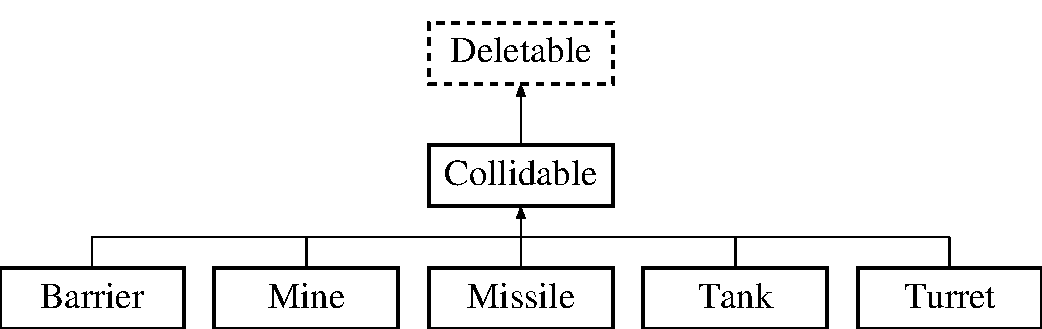
\includegraphics[height=3.000000cm]{classCollidable}
\end{center}
\end{figure}
\subsection*{Public Member Functions}
\begin{DoxyCompactItemize}
\item 
\hyperlink{classCollidable_a92ce9e2b08086bb2f466168ffc69c9ed}{Collidable} ()
\begin{DoxyCompactList}\small\item\em Constructor. \end{DoxyCompactList}\item 
virtual const \hyperlink{structrect__corners}{rect\-\_\-corners} \& \hyperlink{classCollidable_a3436effdcd9bea230f4a1aa32b8dd8ab}{get\-Bounding\-Box} ()=0
\begin{DoxyCompactList}\small\item\em Get bounding box of entity. \end{DoxyCompactList}\item 
virtual const \hyperlink{structrect__corners}{rect\-\_\-corners} \& \hyperlink{classCollidable_a6909df57a0915f044d5d967a3be086f3}{get\-Aligned\-Bounding\-Box} ()=0
\begin{DoxyCompactList}\small\item\em Get Axis Aligned bounding box of entity. \end{DoxyCompactList}\item 
virtual const int \hyperlink{classCollidable_a6d312198ba82d26b5e360733bb87a2f0}{set\-Blocked} (const \hyperlink{Structures_8h_a6fef29d9424addfa69bdd2a379424896}{blocked\-\_\-status} obstruction\-\_\-type)=0
\begin{DoxyCompactList}\small\item\em Set blocked state of entity. \end{DoxyCompactList}\item 
virtual void \hyperlink{classCollidable_a817d864d0640bc6bcb13bbecf14ddf31}{set\-Unblocked} ()=0
\begin{DoxyCompactList}\small\item\em Unset the blocked state of the entity. \end{DoxyCompactList}\item 
virtual void \hyperlink{classCollidable_a5ea0417bea000712171bbe5531705082}{set\-Collided} ()=0
\begin{DoxyCompactList}\small\item\em Set collision state of entity. \end{DoxyCompactList}\item 
virtual \hyperlink{classCollidable_ab742fb86ee54c44b706713b0d6876af7}{$\sim$\-Collidable} ()=0
\begin{DoxyCompactList}\small\item\em Destructor. \end{DoxyCompactList}\end{DoxyCompactItemize}


\subsection{Detailed Description}


Definition at line 21 of file Collidable.\-h.



\subsection{Constructor \& Destructor Documentation}
\hypertarget{classCollidable_a92ce9e2b08086bb2f466168ffc69c9ed}{\index{Collidable@{Collidable}!Collidable@{Collidable}}
\index{Collidable@{Collidable}!Collidable@{Collidable}}
\subsubsection[{Collidable}]{\setlength{\rightskip}{0pt plus 5cm}Collidable\-::\-Collidable (
\begin{DoxyParamCaption}
{}
\end{DoxyParamCaption}
)}}\label{classCollidable_a92ce9e2b08086bb2f466168ffc69c9ed}


Constructor. 



Definition at line 15 of file Collidable.\-cpp.


\begin{DoxyCode}
16 \{
17 
18 \}
\end{DoxyCode}
\hypertarget{classCollidable_ab742fb86ee54c44b706713b0d6876af7}{\index{Collidable@{Collidable}!$\sim$\-Collidable@{$\sim$\-Collidable}}
\index{$\sim$\-Collidable@{$\sim$\-Collidable}!Collidable@{Collidable}}
\subsubsection[{$\sim$\-Collidable}]{\setlength{\rightskip}{0pt plus 5cm}Collidable\-::$\sim$\-Collidable (
\begin{DoxyParamCaption}
{}
\end{DoxyParamCaption}
)\hspace{0.3cm}{\ttfamily [pure virtual]}}}\label{classCollidable_ab742fb86ee54c44b706713b0d6876af7}


Destructor. 



Definition at line 21 of file Collidable.\-cpp.


\begin{DoxyCode}
22 \{
23 
24 \}
\end{DoxyCode}


\subsection{Member Function Documentation}
\hypertarget{classCollidable_a6909df57a0915f044d5d967a3be086f3}{\index{Collidable@{Collidable}!get\-Aligned\-Bounding\-Box@{get\-Aligned\-Bounding\-Box}}
\index{get\-Aligned\-Bounding\-Box@{get\-Aligned\-Bounding\-Box}!Collidable@{Collidable}}
\subsubsection[{get\-Aligned\-Bounding\-Box}]{\setlength{\rightskip}{0pt plus 5cm}virtual const {\bf rect\-\_\-corners}\& Collidable\-::get\-Aligned\-Bounding\-Box (
\begin{DoxyParamCaption}
{}
\end{DoxyParamCaption}
)\hspace{0.3cm}{\ttfamily [pure virtual]}}}\label{classCollidable_a6909df57a0915f044d5d967a3be086f3}


Get Axis Aligned bounding box of entity. 



Implemented in \hyperlink{classTank_acacf07f1695303387f1f6b52fd2e2abb}{Tank}, \hyperlink{classMissile_af2a9b1f8503cc2d322f5ab6ea788d393}{Missile}, \hyperlink{classTurret_ad17a5c236d681627bbea6bb99b2374b0}{Turret}, \hyperlink{classBarrier_a5fe813c8e78457566a5ff61235c12ea6}{Barrier}, and \hyperlink{classMine_a94667c68518d45d9c841501924a83612}{Mine}.

\hypertarget{classCollidable_a3436effdcd9bea230f4a1aa32b8dd8ab}{\index{Collidable@{Collidable}!get\-Bounding\-Box@{get\-Bounding\-Box}}
\index{get\-Bounding\-Box@{get\-Bounding\-Box}!Collidable@{Collidable}}
\subsubsection[{get\-Bounding\-Box}]{\setlength{\rightskip}{0pt plus 5cm}virtual const {\bf rect\-\_\-corners}\& Collidable\-::get\-Bounding\-Box (
\begin{DoxyParamCaption}
{}
\end{DoxyParamCaption}
)\hspace{0.3cm}{\ttfamily [pure virtual]}}}\label{classCollidable_a3436effdcd9bea230f4a1aa32b8dd8ab}


Get bounding box of entity. 



Implemented in \hyperlink{classTank_aeed31f7dcffb3209928a6774c9ec2a16}{Tank}, \hyperlink{classMissile_a6f9a14b7e2a2041fbccb566bf2a3b469}{Missile}, \hyperlink{classTurret_a48007e1c8b99645e13b24e24b850fbaa}{Turret}, \hyperlink{classBarrier_a050de6c9ffbb0a321c6d8a2e3d1dd418}{Barrier}, and \hyperlink{classMine_a36b2ba160a413d45c9743447f075e99e}{Mine}.

\hypertarget{classCollidable_a6d312198ba82d26b5e360733bb87a2f0}{\index{Collidable@{Collidable}!set\-Blocked@{set\-Blocked}}
\index{set\-Blocked@{set\-Blocked}!Collidable@{Collidable}}
\subsubsection[{set\-Blocked}]{\setlength{\rightskip}{0pt plus 5cm}virtual const int Collidable\-::set\-Blocked (
\begin{DoxyParamCaption}
\item[{const {\bf blocked\-\_\-status}}]{obstruction\-\_\-type}
\end{DoxyParamCaption}
)\hspace{0.3cm}{\ttfamily [pure virtual]}}}\label{classCollidable_a6d312198ba82d26b5e360733bb87a2f0}


Set blocked state of entity. 



Implemented in \hyperlink{classTank_a7bedf67f1ae11382f84a3784d9324e60}{Tank}, \hyperlink{classMissile_a4f6e73f8d9f9723a777875efcb9edfa7}{Missile}, \hyperlink{classTurret_a047fe39c0367cc0896c43ac6fadfd2b6}{Turret}, \hyperlink{classBarrier_acff61ab4742c427abdf0d46abd52c832}{Barrier}, and \hyperlink{classMine_acf2add61f1763222f0d1a7333d2b0633}{Mine}.

\hypertarget{classCollidable_a5ea0417bea000712171bbe5531705082}{\index{Collidable@{Collidable}!set\-Collided@{set\-Collided}}
\index{set\-Collided@{set\-Collided}!Collidable@{Collidable}}
\subsubsection[{set\-Collided}]{\setlength{\rightskip}{0pt plus 5cm}virtual void Collidable\-::set\-Collided (
\begin{DoxyParamCaption}
{}
\end{DoxyParamCaption}
)\hspace{0.3cm}{\ttfamily [pure virtual]}}}\label{classCollidable_a5ea0417bea000712171bbe5531705082}


Set collision state of entity. 



Implemented in \hyperlink{classTank_a6e06f183cb856f201a7e5790b852f6a6}{Tank}, \hyperlink{classMissile_a1a27cc48265f34e3298c780c37ca8a0e}{Missile}, \hyperlink{classTurret_a2f558a151cc9c7e7f2158c71f71261cb}{Turret}, \hyperlink{classBarrier_adeedae22d7df279613359026ecf9f279}{Barrier}, and \hyperlink{classMine_a3a51fbecfcb177529bee4b7e13dd75e2}{Mine}.

\hypertarget{classCollidable_a817d864d0640bc6bcb13bbecf14ddf31}{\index{Collidable@{Collidable}!set\-Unblocked@{set\-Unblocked}}
\index{set\-Unblocked@{set\-Unblocked}!Collidable@{Collidable}}
\subsubsection[{set\-Unblocked}]{\setlength{\rightskip}{0pt plus 5cm}virtual void Collidable\-::set\-Unblocked (
\begin{DoxyParamCaption}
{}
\end{DoxyParamCaption}
)\hspace{0.3cm}{\ttfamily [pure virtual]}}}\label{classCollidable_a817d864d0640bc6bcb13bbecf14ddf31}


Unset the blocked state of the entity. 



Implemented in \hyperlink{classTank_a5cbdf86621634b0c698edc5abe1a6d5b}{Tank}, \hyperlink{classMissile_af66d762c4401061f64bcf9b46343c967}{Missile}, \hyperlink{classTurret_a1cafbfb89d052d03c8e7db8b0668a75d}{Turret}, \hyperlink{classBarrier_a863ef65ef677abdcf97373157f86c138}{Barrier}, and \hyperlink{classMine_a859fd28c2c57a37b22ec3b88806f1134}{Mine}.



The documentation for this class was generated from the following files\-:\begin{DoxyCompactItemize}
\item 
\hyperlink{Collidable_8h}{Collidable.\-h}\item 
\hyperlink{Collidable_8cpp}{Collidable.\-cpp}\end{DoxyCompactItemize}

\hypertarget{classCollisionManager}{\section{Collision\-Manager Class Reference}
\label{classCollisionManager}\index{Collision\-Manager@{Collision\-Manager}}
}


\hyperlink{classManager}{Manager} class responsible for managing collisions.  




{\ttfamily \#include $<$Collision\-Manager.\-h$>$}

Inheritance diagram for Collision\-Manager\-:\begin{figure}[H]
\begin{center}
\leavevmode
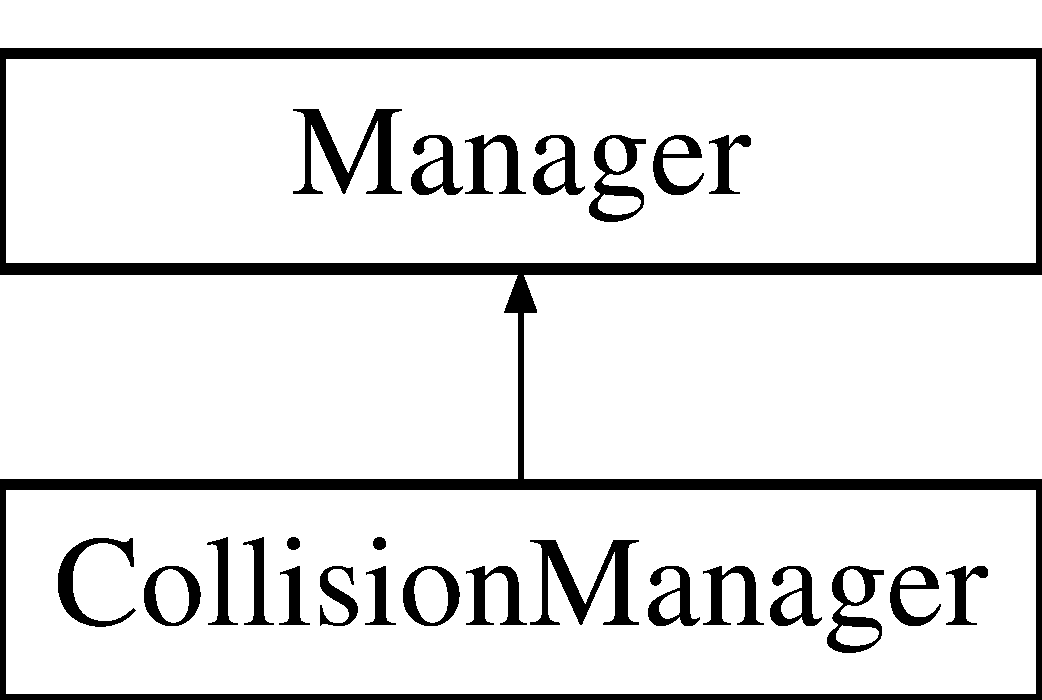
\includegraphics[height=2.000000cm]{classCollisionManager}
\end{center}
\end{figure}
\subsection*{Public Member Functions}
\begin{DoxyCompactItemize}
\item 
\hyperlink{classCollisionManager_a81f0b3f0cc0268c80f54714cd7ddb55f}{Collision\-Manager} ()
\item 
void \hyperlink{classCollisionManager_a43a05dc775565d23ecfaa1fb2638f6cf}{manage} ()
\begin{DoxyCompactList}\small\item\em Checks and sets the collision status of all game entities. \end{DoxyCompactList}\item 
void \hyperlink{classCollisionManager_a2ffe03a672702b8f33d8991b5d631e16}{add\-New\-Entity} (std\-::weak\-\_\-ptr$<$ \hyperlink{classCollidable}{Collidable} $>$ new\-\_\-entity)
\begin{DoxyCompactList}\small\item\em Add new entity to collidables. \end{DoxyCompactList}\item 
virtual \hyperlink{classCollisionManager_acdbb3c842f0ef1c7a028d3f080855766}{$\sim$\-Collision\-Manager} ()
\end{DoxyCompactItemize}
\subsection*{Private Member Functions}
\begin{DoxyCompactItemize}
\item 
const \hyperlink{Structures_8h_a6fef29d9424addfa69bdd2a379424896}{blocked\-\_\-status} \hyperlink{classCollisionManager_a9863f3588677449e9b5edd42aa5bbabd}{get\-Resulting\-Blocked\-Status} (std\-::shared\-\_\-ptr$<$ \hyperlink{classCollidable}{Collidable} $>$ entity\-\_\-1, std\-::shared\-\_\-ptr$<$ \hyperlink{classCollidable}{Collidable} $>$ entity\-\_\-2)
\begin{DoxyCompactList}\small\item\em Set the collision or blocked states for a barrier collision. \end{DoxyCompactList}\item 
void \hyperlink{classCollisionManager_a84a4ba8a52652b2c7164638f937243c1}{review\-Collision\-States} (std\-::shared\-\_\-ptr$<$ \hyperlink{classCollidable}{Collidable} $>$ entity\-\_\-sp, std\-::shared\-\_\-ptr$<$ \hyperlink{classCollidable}{Collidable} $>$ obstacle\-\_\-sp, bool \&entity\-\_\-blocked\-\_\-status)
\begin{DoxyCompactList}\small\item\em Checks to see if two objects have collided base upon their bounding box locations and type. \end{DoxyCompactList}\item 
void \hyperlink{classCollisionManager_a12e52b665a471debc0887deac979ca95}{set\-Collision\-States} (std\-::shared\-\_\-ptr$<$ \hyperlink{classCollidable}{Collidable} $>$ entity\-\_\-1, std\-::shared\-\_\-ptr$<$ \hyperlink{classCollidable}{Collidable} $>$ entity\-\_\-2)
\begin{DoxyCompactList}\small\item\em Set collision state based on the types of entities that have collided. \end{DoxyCompactList}\item 
void \hyperlink{classCollisionManager_aace76303f3c3c2097f9794e42fdbe47d}{tank\-Collision\-Reaction} (std\-::shared\-\_\-ptr$<$ \hyperlink{classCollidable}{Collidable} $>$ entity\-\_\-1, std\-::shared\-\_\-ptr$<$ \hyperlink{classCollidable}{Collidable} $>$ entity\-\_\-2)
\begin{DoxyCompactList}\small\item\em Implement logic when a tank has collided with a game entity. \end{DoxyCompactList}\item 
void \hyperlink{classCollisionManager_a24cc244fbd482cb7de2585878fee2c89}{missile\-Collision\-Reaction} (std\-::shared\-\_\-ptr$<$ \hyperlink{classCollidable}{Collidable} $>$ entity\-\_\-1, std\-::shared\-\_\-ptr$<$ \hyperlink{classCollidable}{Collidable} $>$ entity\-\_\-2)
\begin{DoxyCompactList}\small\item\em Implement logic when a missile has collided with a game entity. \end{DoxyCompactList}\item 
void \hyperlink{classCollisionManager_ad94c2efb613059b9fc66c00b1947e7de}{mine\-Collision\-Reaction} (std\-::shared\-\_\-ptr$<$ \hyperlink{classCollidable}{Collidable} $>$ entity\-\_\-1, std\-::shared\-\_\-ptr$<$ \hyperlink{classCollidable}{Collidable} $>$ entity\-\_\-2)
\begin{DoxyCompactList}\small\item\em Implement logic when a mine has collided with a game entity. \end{DoxyCompactList}\item 
void \hyperlink{classCollisionManager_aa06b6597bf3b4636b55e4bad6a641de2}{barrier\-Collision\-Reaction} (std\-::shared\-\_\-ptr$<$ \hyperlink{classCollidable}{Collidable} $>$ entity\-\_\-1, std\-::shared\-\_\-ptr$<$ \hyperlink{classCollidable}{Collidable} $>$ entity\-\_\-2)
\begin{DoxyCompactList}\small\item\em Implement logic when a barrier has been collided with a game entity. \end{DoxyCompactList}\item 
void \hyperlink{classCollisionManager_ad175a3730f4c984adae73814706417de}{turret\-Collision\-Reaction} (std\-::shared\-\_\-ptr$<$ \hyperlink{classCollidable}{Collidable} $>$ entity\-\_\-1, std\-::shared\-\_\-ptr$<$ \hyperlink{classCollidable}{Collidable} $>$ entity\-\_\-2)
\begin{DoxyCompactList}\small\item\em Implement logic when a turret has collided with a game entity. \end{DoxyCompactList}\item 
void \hyperlink{classCollisionManager_a06e15e9c05a1ae1742a71e6b8b72629a}{turret\-Missile\-Collision\-Reaction} (std\-::shared\-\_\-ptr$<$ \hyperlink{classCollidable}{Collidable} $>$ entity\-\_\-1, std\-::shared\-\_\-ptr$<$ \hyperlink{classCollidable}{Collidable} $>$ entity\-\_\-2)
\begin{DoxyCompactList}\small\item\em Implement logic when a turret missile has collided with a game entity. \end{DoxyCompactList}\item 
void \hyperlink{classCollisionManager_a2d1b6195cdcdf6a0ccf7804baf98c71e}{reset\-Blocked\-State} (std\-::shared\-\_\-ptr$<$ \hyperlink{classCollidable}{Collidable} $>$ \&entity)
\begin{DoxyCompactList}\small\item\em Resets the blocked states of blocks that were previously blocked, but are not colliding with anything. \end{DoxyCompactList}\item 
void \hyperlink{classCollisionManager_a8f18fb2f3086dc63603b79afe3f5dc9b}{remove\-Garbage} ()
\begin{DoxyCompactList}\small\item\em Helper function to remove 'Dead' entities from collision manager. \end{DoxyCompactList}\end{DoxyCompactItemize}
\subsection*{Private Attributes}
\begin{DoxyCompactItemize}
\item 
std\-::vector$<$ std\-::weak\-\_\-ptr\\*
$<$ \hyperlink{classCollidable}{Collidable} $>$ $>$ \hyperlink{classCollisionManager_a2a05a1861c85c833f8d229de43a00bb4}{\-\_\-collidables}
\begin{DoxyCompactList}\small\item\em Pointers to all collidable entities within the game world. \end{DoxyCompactList}\end{DoxyCompactItemize}


\subsection{Detailed Description}
\hyperlink{classManager}{Manager} class responsible for managing collisions. 

Definition at line 20 of file Collision\-Manager.\-h.



\subsection{Constructor \& Destructor Documentation}
\hypertarget{classCollisionManager_a81f0b3f0cc0268c80f54714cd7ddb55f}{\index{Collision\-Manager@{Collision\-Manager}!Collision\-Manager@{Collision\-Manager}}
\index{Collision\-Manager@{Collision\-Manager}!CollisionManager@{Collision\-Manager}}
\subsubsection[{Collision\-Manager}]{\setlength{\rightskip}{0pt plus 5cm}Collision\-Manager\-::\-Collision\-Manager (
\begin{DoxyParamCaption}
{}
\end{DoxyParamCaption}
)}}\label{classCollisionManager_a81f0b3f0cc0268c80f54714cd7ddb55f}


Definition at line 15 of file Collision\-Manager.\-cpp.


\begin{DoxyCode}
16 \{
17 
18 \}
\end{DoxyCode}
\hypertarget{classCollisionManager_acdbb3c842f0ef1c7a028d3f080855766}{\index{Collision\-Manager@{Collision\-Manager}!$\sim$\-Collision\-Manager@{$\sim$\-Collision\-Manager}}
\index{$\sim$\-Collision\-Manager@{$\sim$\-Collision\-Manager}!CollisionManager@{Collision\-Manager}}
\subsubsection[{$\sim$\-Collision\-Manager}]{\setlength{\rightskip}{0pt plus 5cm}Collision\-Manager\-::$\sim$\-Collision\-Manager (
\begin{DoxyParamCaption}
{}
\end{DoxyParamCaption}
)\hspace{0.3cm}{\ttfamily [virtual]}}}\label{classCollisionManager_acdbb3c842f0ef1c7a028d3f080855766}


Definition at line 431 of file Collision\-Manager.\-cpp.


\begin{DoxyCode}
432 \{
433 
434 \}
\end{DoxyCode}


\subsection{Member Function Documentation}
\hypertarget{classCollisionManager_a2ffe03a672702b8f33d8991b5d631e16}{\index{Collision\-Manager@{Collision\-Manager}!add\-New\-Entity@{add\-New\-Entity}}
\index{add\-New\-Entity@{add\-New\-Entity}!CollisionManager@{Collision\-Manager}}
\subsubsection[{add\-New\-Entity}]{\setlength{\rightskip}{0pt plus 5cm}void Collision\-Manager\-::add\-New\-Entity (
\begin{DoxyParamCaption}
\item[{std\-::weak\-\_\-ptr$<$ {\bf Collidable} $>$}]{new\-\_\-entity}
\end{DoxyParamCaption}
)}}\label{classCollisionManager_a2ffe03a672702b8f33d8991b5d631e16}


Add new entity to collidables. 

A new entity is added to the private collidables vector, which is used in the main manage function. 
\begin{DoxyParams}{Parameters}
{\em new\-\_\-entity} & \-:\-: Entity to be added to collidables vector \\
\hline
\end{DoxyParams}


Definition at line 109 of file Collision\-Manager.\-cpp.



References \-\_\-collidables.



Referenced by Game\-::add\-Collidable(), main(), and T\-E\-S\-T().


\begin{DoxyCode}
110 \{
111     \hyperlink{classCollisionManager_a2a05a1861c85c833f8d229de43a00bb4}{\_collidables}.push\_back(new\_entity);
112 \}
\end{DoxyCode}
\hypertarget{classCollisionManager_aa06b6597bf3b4636b55e4bad6a641de2}{\index{Collision\-Manager@{Collision\-Manager}!barrier\-Collision\-Reaction@{barrier\-Collision\-Reaction}}
\index{barrier\-Collision\-Reaction@{barrier\-Collision\-Reaction}!CollisionManager@{Collision\-Manager}}
\subsubsection[{barrier\-Collision\-Reaction}]{\setlength{\rightskip}{0pt plus 5cm}void Collision\-Manager\-::barrier\-Collision\-Reaction (
\begin{DoxyParamCaption}
\item[{std\-::shared\-\_\-ptr$<$ {\bf Collidable} $>$}]{entity\-\_\-1, }
\item[{std\-::shared\-\_\-ptr$<$ {\bf Collidable} $>$}]{entity\-\_\-2}
\end{DoxyParamCaption}
)\hspace{0.3cm}{\ttfamily [private]}}}\label{classCollisionManager_aa06b6597bf3b4636b55e4bad6a641de2}


Implement logic when a barrier has been collided with a game entity. 


\begin{DoxyParams}{Parameters}
{\em entity\-\_\-1} & \-:\-: First entity that will have its status changed \\
\hline
{\em entity\-\_\-2} & \-:\-: Second entity that will have its status changed \\
\hline
\end{DoxyParams}


Definition at line 149 of file Collision\-Manager.\-cpp.



References blocked, get\-Resulting\-Blocked\-Status(), p1\-\_\-mine, p1\-\_\-missile, p1\-\_\-tank, p2\-\_\-mine, p2\-\_\-missile, and p2\-\_\-tank.



Referenced by set\-Collision\-States().


\begin{DoxyCode}
150 \{
151     \textcolor{keywordflow}{switch}(entity\_2->getType())
152     \{
153     \textcolor{keywordflow}{case} \hyperlink{Structures_8h_a6d8f83e710b27d4f86c45f0bb77066e3a31fa78b2b7dd774f5158a16ef230932e}{p1\_tank}:
154         entity\_2->setBlocked(\hyperlink{Structures_8h_a6fef29d9424addfa69bdd2a379424896a9ee4e6c1dfe13f0d0f0cb7b29c62b2eb}{blocked}); \textcolor{comment}{// tank does not move}
155         \textcolor{keywordflow}{break};
156 
157     \textcolor{keywordflow}{case} \hyperlink{Structures_8h_a6d8f83e710b27d4f86c45f0bb77066e3a3d48d62c7b88e7ee171698fe56dc9e59}{p2\_tank}:
158         entity\_2->setBlocked(\hyperlink{Structures_8h_a6fef29d9424addfa69bdd2a379424896a9ee4e6c1dfe13f0d0f0cb7b29c62b2eb}{blocked}); \textcolor{comment}{// tank does not move}
159         \textcolor{keywordflow}{break};
160 
161     \textcolor{keywordflow}{case} \hyperlink{Structures_8h_a6d8f83e710b27d4f86c45f0bb77066e3af89bc631e9b0140ed004b5ce2db5330c}{p1\_missile}:
162         \{
163             entity\_2->setBlocked(\hyperlink{classCollisionManager_a9863f3588677449e9b5edd42aa5bbabd}{getResultingBlockedStatus}(entity\_2, entity\_1)); \textcolor{comment}{
      // missile rebounds}
164         \}
165         \textcolor{keywordflow}{break};
166 
167     \textcolor{keywordflow}{case} \hyperlink{Structures_8h_a6d8f83e710b27d4f86c45f0bb77066e3a47100170e5852d632dfe65582a18256d}{p2\_missile}:
168         \{
169             entity\_2->setBlocked(\hyperlink{classCollisionManager_a9863f3588677449e9b5edd42aa5bbabd}{getResultingBlockedStatus}(entity\_2, entity\_1)); \textcolor{comment}{
      // missile rebounds}
170         \}
171         \textcolor{keywordflow}{break};
172 
173     \textcolor{keywordflow}{case} \hyperlink{Structures_8h_a6d8f83e710b27d4f86c45f0bb77066e3afc52e626787e982ae5d0a747bed6666d}{p1\_mine}:
174         entity\_2->setCollided();
175         \textcolor{keywordflow}{break};
176 
177     \textcolor{keywordflow}{case} \hyperlink{Structures_8h_a6d8f83e710b27d4f86c45f0bb77066e3ada293b37940e64ec2cf6dbd2ae493d2b}{p2\_mine}:
178         entity\_2->setCollided();
179         \textcolor{keywordflow}{break};
180 
181     \textcolor{keywordflow}{default}:
182         \textcolor{keywordflow}{break};
183     \}\textcolor{comment}{//Switch}
184 
185 \}
\end{DoxyCode}
\hypertarget{classCollisionManager_a9863f3588677449e9b5edd42aa5bbabd}{\index{Collision\-Manager@{Collision\-Manager}!get\-Resulting\-Blocked\-Status@{get\-Resulting\-Blocked\-Status}}
\index{get\-Resulting\-Blocked\-Status@{get\-Resulting\-Blocked\-Status}!CollisionManager@{Collision\-Manager}}
\subsubsection[{get\-Resulting\-Blocked\-Status}]{\setlength{\rightskip}{0pt plus 5cm}const {\bf blocked\-\_\-status} Collision\-Manager\-::get\-Resulting\-Blocked\-Status (
\begin{DoxyParamCaption}
\item[{std\-::shared\-\_\-ptr$<$ {\bf Collidable} $>$}]{entity\-\_\-1, }
\item[{std\-::shared\-\_\-ptr$<$ {\bf Collidable} $>$}]{entity\-\_\-2}
\end{DoxyParamCaption}
)\hspace{0.3cm}{\ttfamily [private]}}}\label{classCollisionManager_a9863f3588677449e9b5edd42aa5bbabd}


Set the collision or blocked states for a barrier collision. 


\begin{DoxyParams}{Parameters}
{\em entity\-\_\-1} & \-:\-: First entity that will have its status changed \\
\hline
{\em entity\-\_\-2} & \-:\-: Second entity that will have its status changed \\
\hline
\end{DoxyParams}
\begin{DoxyReturn}{Returns}
blocked\-\_\-status 
\end{DoxyReturn}


Definition at line 352 of file Collision\-Manager.\-cpp.



References Geometry\-Engine\-::get\-Relative\-Position().



Referenced by barrier\-Collision\-Reaction(), and missile\-Collision\-Reaction().


\begin{DoxyCode}
353 \{
354     \textcolor{keyword}{auto} entity\_collision\_box = entity\_1->getAlignedBoundingBox();
355     \textcolor{keyword}{auto} object\_collision\_box = entity\_2->getAlignedBoundingBox();
356     \hyperlink{classGeometryEngine}{GeometryEngine} geometry\_engine;
357     \textcolor{keywordflow}{return} (geometry\_engine.\hyperlink{classGeometryEngine_a662ec9af09fd513700f41d3e7090b1bf}{getRelativePosition}(entity\_collision\_box,
      object\_collision\_box));
358 \}
\end{DoxyCode}
\hypertarget{classCollisionManager_a43a05dc775565d23ecfaa1fb2638f6cf}{\index{Collision\-Manager@{Collision\-Manager}!manage@{manage}}
\index{manage@{manage}!CollisionManager@{Collision\-Manager}}
\subsubsection[{manage}]{\setlength{\rightskip}{0pt plus 5cm}void Collision\-Manager\-::manage (
\begin{DoxyParamCaption}
{}
\end{DoxyParamCaption}
)}}\label{classCollisionManager_a43a05dc775565d23ecfaa1fb2638f6cf}


Checks and sets the collision status of all game entities. 

This is the main function of the \hyperlink{classCollisionManager}{Collision\-Manager}. The manager iterates through all of the collidables and checks it against every other collidable to see if a collision has taken place. If an entity that needs to be compared to another entity is blocked, it's status is temporarily set as false so that a proper comparison can be made. This entity is the entity of the outer for loop. 

Definition at line 27 of file Collision\-Manager.\-cpp.



References \-\_\-collidables, remove\-Garbage(), and review\-Collision\-States().



Referenced by main(), Game\-::run\-All\-Managers(), and T\-E\-S\-T().


\begin{DoxyCode}
28 \{
29 
30     \textcolor{comment}{//Clear all deleted entities from the \_collidables vector}
31     \hyperlink{classCollisionManager_a8f18fb2f3086dc63603b79afe3f5dc9b}{removeGarbage}();
32 
33     \textcolor{comment}{//Iterator at initial position within vector}
34     \textcolor{keyword}{auto} i = \hyperlink{classCollisionManager_a2a05a1861c85c833f8d229de43a00bb4}{\_collidables}.begin();
35     \textcolor{keywordflow}{for} (; i != \hyperlink{classCollisionManager_a2a05a1861c85c833f8d229de43a00bb4}{\_collidables}.end(); ++i)
36     \{
37         \textcolor{keywordtype}{bool} entity\_blocked = \textcolor{keyword}{false};
38         std::weak\_ptr<Collidable> entity\_wp = (*i);
39         \textcolor{comment}{//Convert weak\_ptr to shared\_ptr}
40         std::shared\_ptr<Collidable> entity\_sp = entity\_wp.lock();
41 
42         \textcolor{comment}{//Loop through vector of itterators again}
43         \textcolor{keyword}{auto} j = \hyperlink{classCollisionManager_a2a05a1861c85c833f8d229de43a00bb4}{\_collidables}.begin();
44         \textcolor{keywordflow}{for} (; j != \hyperlink{classCollisionManager_a2a05a1861c85c833f8d229de43a00bb4}{\_collidables}.end(); ++j)
45         \{
46             \textcolor{keywordflow}{if} (i != j)
47             \{
48                 std::weak\_ptr<Collidable> obstacle\_wp = (*j);
49                 \textcolor{comment}{//Convert weak\_ptr to shared\_ptr}
50                 std::shared\_ptr<Collidable> obstacle\_sp = obstacle\_wp.lock();
51 
52                 \hyperlink{classCollisionManager_a84a4ba8a52652b2c7164638f937243c1}{reviewCollisionStates}(entity\_sp, obstacle\_sp, entity\_blocked);
53             \}\textcolor{comment}{// if}
54         \}\textcolor{comment}{//inner-for}
55     \}\textcolor{comment}{//outer-for}
56 \}\textcolor{comment}{//Manage function}
\end{DoxyCode}
\hypertarget{classCollisionManager_ad94c2efb613059b9fc66c00b1947e7de}{\index{Collision\-Manager@{Collision\-Manager}!mine\-Collision\-Reaction@{mine\-Collision\-Reaction}}
\index{mine\-Collision\-Reaction@{mine\-Collision\-Reaction}!CollisionManager@{Collision\-Manager}}
\subsubsection[{mine\-Collision\-Reaction}]{\setlength{\rightskip}{0pt plus 5cm}void Collision\-Manager\-::mine\-Collision\-Reaction (
\begin{DoxyParamCaption}
\item[{std\-::shared\-\_\-ptr$<$ {\bf Collidable} $>$}]{entity\-\_\-1, }
\item[{std\-::shared\-\_\-ptr$<$ {\bf Collidable} $>$}]{entity\-\_\-2}
\end{DoxyParamCaption}
)\hspace{0.3cm}{\ttfamily [private]}}}\label{classCollisionManager_ad94c2efb613059b9fc66c00b1947e7de}


Implement logic when a mine has collided with a game entity. 


\begin{DoxyParams}{Parameters}
{\em entity\-\_\-1} & \-:\-: First entity that will have its status changed \\
\hline
{\em entity\-\_\-2} & \-:\-: Second entity that will have its status changed \\
\hline
\end{DoxyParams}


Definition at line 191 of file Collision\-Manager.\-cpp.



References barrier, p1\-\_\-mine, p1\-\_\-tank, p2\-\_\-mine, p2\-\_\-tank, and turret.



Referenced by set\-Collision\-States().


\begin{DoxyCode}
192 \{
193     \textcolor{keywordflow}{switch}(entity\_2->getType())
194     \{
195     \textcolor{keywordflow}{case} \hyperlink{Structures_8h_a6d8f83e710b27d4f86c45f0bb77066e3a31fa78b2b7dd774f5158a16ef230932e}{p1\_tank}:
196         entity\_1->setCollided(); \textcolor{comment}{// mine}
197         entity\_2->setCollided(); \textcolor{comment}{// tank}
198         \textcolor{keywordflow}{break};
199 
200     \textcolor{keywordflow}{case} \hyperlink{Structures_8h_a6d8f83e710b27d4f86c45f0bb77066e3a3d48d62c7b88e7ee171698fe56dc9e59}{p2\_tank}:
201         entity\_1->setCollided(); \textcolor{comment}{// mine}
202         entity\_2->setCollided(); \textcolor{comment}{// tank}
203         \textcolor{keywordflow}{break};
204 
205     \textcolor{keywordflow}{case} \hyperlink{Structures_8h_a6d8f83e710b27d4f86c45f0bb77066e3a6fb040c958f554e1d8320926b700b59d}{barrier}:
206         entity\_1->setCollided(); \textcolor{comment}{//mine}
207         \textcolor{keywordflow}{break};
208 
209     \textcolor{keywordflow}{case} \hyperlink{Structures_8h_a6d8f83e710b27d4f86c45f0bb77066e3a85c730ac9ffc13ac94e6e860579928a1}{turret}:
210         entity\_1->setCollided();
211         \textcolor{keywordflow}{break};
212 
213     \textcolor{keywordflow}{case} \hyperlink{Structures_8h_a6d8f83e710b27d4f86c45f0bb77066e3afc52e626787e982ae5d0a747bed6666d}{p1\_mine}:
214         entity\_1->setCollided();
215 
216     \textcolor{keywordflow}{case} \hyperlink{Structures_8h_a6d8f83e710b27d4f86c45f0bb77066e3ada293b37940e64ec2cf6dbd2ae493d2b}{p2\_mine}:
217         entity\_1->setCollided();
218 
219     \textcolor{keywordflow}{default}:
220         \textcolor{keywordflow}{break};
221     \}
222 \}
\end{DoxyCode}
\hypertarget{classCollisionManager_a24cc244fbd482cb7de2585878fee2c89}{\index{Collision\-Manager@{Collision\-Manager}!missile\-Collision\-Reaction@{missile\-Collision\-Reaction}}
\index{missile\-Collision\-Reaction@{missile\-Collision\-Reaction}!CollisionManager@{Collision\-Manager}}
\subsubsection[{missile\-Collision\-Reaction}]{\setlength{\rightskip}{0pt plus 5cm}void Collision\-Manager\-::missile\-Collision\-Reaction (
\begin{DoxyParamCaption}
\item[{std\-::shared\-\_\-ptr$<$ {\bf Collidable} $>$}]{entity\-\_\-1, }
\item[{std\-::shared\-\_\-ptr$<$ {\bf Collidable} $>$}]{entity\-\_\-2}
\end{DoxyParamCaption}
)\hspace{0.3cm}{\ttfamily [private]}}}\label{classCollisionManager_a24cc244fbd482cb7de2585878fee2c89}


Implement logic when a missile has collided with a game entity. 


\begin{DoxyParams}{Parameters}
{\em entity\-\_\-1} & \-:\-: First entity that will have its status changed \\
\hline
{\em entity\-\_\-2} & \-:\-: Second entity that will have its status changed \\
\hline
\end{DoxyParams}


Definition at line 228 of file Collision\-Manager.\-cpp.



References barrier, get\-Resulting\-Blocked\-Status(), p1\-\_\-missile, p1\-\_\-tank, p2\-\_\-missile, p2\-\_\-tank, and turret.



Referenced by set\-Collision\-States().


\begin{DoxyCode}
229 \{
230     \textcolor{keywordflow}{switch}(entity\_2->getType())
231     \{
232     \textcolor{keywordflow}{case} \hyperlink{Structures_8h_a6d8f83e710b27d4f86c45f0bb77066e3a31fa78b2b7dd774f5158a16ef230932e}{p1\_tank}:
233         entity\_1->setCollided(); \textcolor{comment}{// missile}
234         entity\_2->setCollided(); \textcolor{comment}{// tank}
235         \textcolor{keywordflow}{break};
236 
237     \textcolor{keywordflow}{case} \hyperlink{Structures_8h_a6d8f83e710b27d4f86c45f0bb77066e3a3d48d62c7b88e7ee171698fe56dc9e59}{p2\_tank}:
238         entity\_1->setCollided(); \textcolor{comment}{// missile}
239         entity\_2->setCollided(); \textcolor{comment}{// tank}
240         \textcolor{keywordflow}{break};
241 
242     \textcolor{keywordflow}{case} \hyperlink{Structures_8h_a6d8f83e710b27d4f86c45f0bb77066e3a85c730ac9ffc13ac94e6e860579928a1}{turret}:
243         entity\_1->setCollided(); \textcolor{comment}{// turret}
244         entity\_2->setCollided(); \textcolor{comment}{// missile}
245 
246     \textcolor{keywordflow}{case} \hyperlink{Structures_8h_a6d8f83e710b27d4f86c45f0bb77066e3af89bc631e9b0140ed004b5ce2db5330c}{p1\_missile}:
247         entity\_1->setCollided(); \textcolor{comment}{// missile}
248         entity\_2->setCollided(); \textcolor{comment}{// missile}
249         \textcolor{keywordflow}{break};
250 
251     \textcolor{keywordflow}{case} \hyperlink{Structures_8h_a6d8f83e710b27d4f86c45f0bb77066e3a47100170e5852d632dfe65582a18256d}{p2\_missile}:
252         entity\_1->setCollided(); \textcolor{comment}{// missile}
253         entity\_2->setCollided(); \textcolor{comment}{// missile}
254         \textcolor{keywordflow}{break};
255 
256     \textcolor{keywordflow}{case} \hyperlink{Structures_8h_a6d8f83e710b27d4f86c45f0bb77066e3a6fb040c958f554e1d8320926b700b59d}{barrier}:
257         \textcolor{keywordflow}{if} (entity\_1->setBlocked(\hyperlink{classCollisionManager_a9863f3588677449e9b5edd42aa5bbabd}{getResultingBlockedStatus}(entity\_1, entity\_2)) <=
       0) \textcolor{comment}{// missile}
258             entity\_1->setCollided();
259         \textcolor{keywordflow}{break};
260 
261     \textcolor{keywordflow}{default}:
262         \textcolor{keywordflow}{break};
263     \}
264 \}
\end{DoxyCode}
\hypertarget{classCollisionManager_a8f18fb2f3086dc63603b79afe3f5dc9b}{\index{Collision\-Manager@{Collision\-Manager}!remove\-Garbage@{remove\-Garbage}}
\index{remove\-Garbage@{remove\-Garbage}!CollisionManager@{Collision\-Manager}}
\subsubsection[{remove\-Garbage}]{\setlength{\rightskip}{0pt plus 5cm}void Collision\-Manager\-::remove\-Garbage (
\begin{DoxyParamCaption}
{}
\end{DoxyParamCaption}
)\hspace{0.3cm}{\ttfamily [private]}}}\label{classCollisionManager_a8f18fb2f3086dc63603b79afe3f5dc9b}


Helper function to remove 'Dead' entities from collision manager. 



Definition at line 411 of file Collision\-Manager.\-cpp.



References \-\_\-collidables.



Referenced by manage().


\begin{DoxyCode}
412 \{
413     \textcolor{keyword}{auto} removal = \hyperlink{classCollisionManager_a2a05a1861c85c833f8d229de43a00bb4}{\_collidables}.begin();
414     \textcolor{keywordflow}{for} (; removal != \hyperlink{classCollisionManager_a2a05a1861c85c833f8d229de43a00bb4}{\_collidables}.end();)
415     \{
416         std::weak\_ptr<Collidable> removal\_wp = (*removal);
417         \textcolor{comment}{//Convert weak\_ptr to shared\_ptr}
418         std::shared\_ptr<Collidable> removal\_sp = removal\_wp.lock();
419         \textcolor{comment}{//Test if pointer still valid}
420         \textcolor{keywordflow}{if}(removal\_sp)
421         \{
422             removal++;
423         \}
424         \textcolor{keywordflow}{else}
425         \{
426             \hyperlink{classCollisionManager_a2a05a1861c85c833f8d229de43a00bb4}{\_collidables}.erase(removal);
427         \}
428     \}
429 \}
\end{DoxyCode}
\hypertarget{classCollisionManager_a2d1b6195cdcdf6a0ccf7804baf98c71e}{\index{Collision\-Manager@{Collision\-Manager}!reset\-Blocked\-State@{reset\-Blocked\-State}}
\index{reset\-Blocked\-State@{reset\-Blocked\-State}!CollisionManager@{Collision\-Manager}}
\subsubsection[{reset\-Blocked\-State}]{\setlength{\rightskip}{0pt plus 5cm}void Collision\-Manager\-::reset\-Blocked\-State (
\begin{DoxyParamCaption}
\item[{std\-::shared\-\_\-ptr$<$ {\bf Collidable} $>$ \&}]{entity}
\end{DoxyParamCaption}
)\hspace{0.3cm}{\ttfamily [private]}}}\label{classCollisionManager_a2d1b6195cdcdf6a0ccf7804baf98c71e}


Resets the blocked states of blocks that were previously blocked, but are not colliding with anything. 


\begin{DoxyParams}{Parameters}
{\em entity} & \-:\-: entity whose blocked state will be changed \\
\hline
\end{DoxyParams}


Definition at line 99 of file Collision\-Manager.\-cpp.



Referenced by review\-Collision\-States().


\begin{DoxyCode}
100 \{
101     entity->setUnblocked();
102 \}
\end{DoxyCode}
\hypertarget{classCollisionManager_a84a4ba8a52652b2c7164638f937243c1}{\index{Collision\-Manager@{Collision\-Manager}!review\-Collision\-States@{review\-Collision\-States}}
\index{review\-Collision\-States@{review\-Collision\-States}!CollisionManager@{Collision\-Manager}}
\subsubsection[{review\-Collision\-States}]{\setlength{\rightskip}{0pt plus 5cm}void Collision\-Manager\-::review\-Collision\-States (
\begin{DoxyParamCaption}
\item[{std\-::shared\-\_\-ptr$<$ {\bf Collidable} $>$}]{entity\-\_\-sp, }
\item[{std\-::shared\-\_\-ptr$<$ {\bf Collidable} $>$}]{obstacle\-\_\-sp, }
\item[{bool \&}]{entity\-\_\-blocked\-\_\-status}
\end{DoxyParamCaption}
)\hspace{0.3cm}{\ttfamily [private]}}}\label{classCollisionManager_a84a4ba8a52652b2c7164638f937243c1}


Checks to see if two objects have collided base upon their bounding box locations and type. 

This function excludes barriers. All other entities will have their collision states reviewed. The points of the four corners of each entity are used to test if there is a collision. 
\begin{DoxyParams}{Parameters}
{\em entity\-\_\-sp} & \-:\-: Shared pointer to one entity \\
\hline
{\em obstacle\-\_\-sp} & \-:\-: Shared pointer to the other entity \\
\hline
{\em entity\-\_\-blocked\-\_\-status} & \-:\-: blocked status of entity that is being compared to every other entity \\
\hline
\end{DoxyParams}


Definition at line 121 of file Collision\-Manager.\-cpp.



References barrier, Geometry\-Engine\-::is\-Collision(), reset\-Blocked\-State(), and set\-Collision\-States().



Referenced by manage().


\begin{DoxyCode}
124 \{
125     \textcolor{comment}{//This excludes comparing barrier collisions}
126     \textcolor{keywordflow}{if} ((obstacle\_sp->getType() != \hyperlink{Structures_8h_a6d8f83e710b27d4f86c45f0bb77066e3a6fb040c958f554e1d8320926b700b59d}{barrier}) || (entity\_sp->getType() != 
      \hyperlink{Structures_8h_a6d8f83e710b27d4f86c45f0bb77066e3a6fb040c958f554e1d8320926b700b59d}{barrier}))
127     \{
128         \textcolor{keyword}{const} \hyperlink{structrect__corners}{rect\_corners}& entity\_box = (entity\_sp)->getBoundingBox();
129         \textcolor{keyword}{const} \hyperlink{structrect__corners}{rect\_corners}& obstacle\_box = (obstacle\_sp)->getBoundingBox();
130 
131         \hyperlink{classGeometryEngine}{GeometryEngine} geometry\_engine;\textcolor{comment}{// utilise the geometry engine}
132 
133         \textcolor{keywordflow}{if} (geometry\_engine.\hyperlink{classGeometryEngine_a049acffe89f53be25fbc9d4018c3b388}{isCollision}(entity\_box, obstacle\_box))
134         \{
135             entity\_blocked\_status = \textcolor{keyword}{true};
136             \hyperlink{classCollisionManager_a12e52b665a471debc0887deac979ca95}{setCollisionStates}(entity\_sp, obstacle\_sp);
137         \}
138         \textcolor{keywordflow}{if} (!entity\_blocked\_status)
139         \{
140             \hyperlink{classCollisionManager_a2d1b6195cdcdf6a0ccf7804baf98c71e}{resetBlockedState}(entity\_sp);
141         \}
142     \}\textcolor{comment}{//Barrier comparison if}
143 \}
\end{DoxyCode}
\hypertarget{classCollisionManager_a12e52b665a471debc0887deac979ca95}{\index{Collision\-Manager@{Collision\-Manager}!set\-Collision\-States@{set\-Collision\-States}}
\index{set\-Collision\-States@{set\-Collision\-States}!CollisionManager@{Collision\-Manager}}
\subsubsection[{set\-Collision\-States}]{\setlength{\rightskip}{0pt plus 5cm}void Collision\-Manager\-::set\-Collision\-States (
\begin{DoxyParamCaption}
\item[{std\-::shared\-\_\-ptr$<$ {\bf Collidable} $>$}]{entity\-\_\-1, }
\item[{std\-::shared\-\_\-ptr$<$ {\bf Collidable} $>$}]{entity\-\_\-2}
\end{DoxyParamCaption}
)\hspace{0.3cm}{\ttfamily [private]}}}\label{classCollisionManager_a12e52b665a471debc0887deac979ca95}


Set collision state based on the types of entities that have collided. 

Different rules for collision apply to different game entities. Different collision functions are run based on what entities have collided. Rules for collision can be changed or added here. 
\begin{DoxyParams}{Parameters}
{\em entity\-\_\-1} & \-:\-: First entity whose collision state will be set \\
\hline
{\em entity\-\_\-2} & \-:\-: Second entity whose collision state will be set \\
\hline
\end{DoxyParams}


Definition at line 64 of file Collision\-Manager.\-cpp.



References barrier, barrier\-Collision\-Reaction(), mine\-Collision\-Reaction(), missile\-Collision\-Reaction(), p1\-\_\-mine, p1\-\_\-missile, p1\-\_\-tank, p2\-\_\-mine, p2\-\_\-missile, p2\-\_\-tank, tank\-Collision\-Reaction(), turret, turret\-\_\-missile, turret\-Collision\-Reaction(), and turret\-Missile\-Collision\-Reaction().



Referenced by review\-Collision\-States().


\begin{DoxyCode}
65 \{
66     \textcolor{keywordflow}{if} ((entity\_1->getType() == \hyperlink{Structures_8h_a6d8f83e710b27d4f86c45f0bb77066e3a31fa78b2b7dd774f5158a16ef230932e}{p1\_tank}) || (entity\_1->getType() == 
      \hyperlink{Structures_8h_a6d8f83e710b27d4f86c45f0bb77066e3a3d48d62c7b88e7ee171698fe56dc9e59}{p2\_tank}))
67     \{
68         \hyperlink{classCollisionManager_aace76303f3c3c2097f9794e42fdbe47d}{tankCollisionReaction}(entity\_1,entity\_2);
69     \}
70     \textcolor{keywordflow}{else} \textcolor{keywordflow}{if} ((entity\_1->getType() == \hyperlink{Structures_8h_a6d8f83e710b27d4f86c45f0bb77066e3af89bc631e9b0140ed004b5ce2db5330c}{p1\_missile}) ||(entity\_1->getType() == 
      \hyperlink{Structures_8h_a6d8f83e710b27d4f86c45f0bb77066e3a47100170e5852d632dfe65582a18256d}{p2\_missile}))
71     \{
72         \hyperlink{classCollisionManager_a24cc244fbd482cb7de2585878fee2c89}{missileCollisionReaction}(entity\_1,entity\_2);
73     \}
74 
75     \textcolor{keywordflow}{else} \textcolor{keywordflow}{if} ((entity\_1->getType() == \hyperlink{Structures_8h_a6d8f83e710b27d4f86c45f0bb77066e3afc52e626787e982ae5d0a747bed6666d}{p1\_mine}) || (entity\_1->getType() == 
      \hyperlink{Structures_8h_a6d8f83e710b27d4f86c45f0bb77066e3ada293b37940e64ec2cf6dbd2ae493d2b}{p2\_mine}))
76     \{
77         \hyperlink{classCollisionManager_ad94c2efb613059b9fc66c00b1947e7de}{mineCollisionReaction}(entity\_1,entity\_2);
78     \}
79 
80     \textcolor{keywordflow}{else} \textcolor{keywordflow}{if} (entity\_1->getType() == \hyperlink{Structures_8h_a6d8f83e710b27d4f86c45f0bb77066e3a6fb040c958f554e1d8320926b700b59d}{barrier})
81     \{
82         \hyperlink{classCollisionManager_aa06b6597bf3b4636b55e4bad6a641de2}{barrierCollisionReaction}(entity\_1,entity\_2);
83     \}\textcolor{comment}{//Else}
84 
85     \textcolor{keywordflow}{else} \textcolor{keywordflow}{if} (entity\_1->getType() == \hyperlink{Structures_8h_a6d8f83e710b27d4f86c45f0bb77066e3a85c730ac9ffc13ac94e6e860579928a1}{turret})
86     \{
87         \hyperlink{classCollisionManager_ad175a3730f4c984adae73814706417de}{turretCollisionReaction}(entity\_1,entity\_2);
88     \}\textcolor{comment}{//Else}
89 
90         \textcolor{keywordflow}{else} \textcolor{keywordflow}{if} (entity\_1->getType() == \hyperlink{Structures_8h_a6d8f83e710b27d4f86c45f0bb77066e3a8f552a1e495ced5aa8775faa1b6a757b}{turret\_missile})
91     \{
92         \hyperlink{classCollisionManager_a06e15e9c05a1ae1742a71e6b8b72629a}{turretMissileCollisionReaction}(entity\_1,entity\_2);
93     \}\textcolor{comment}{//Else}
94 \}\textcolor{comment}{//Function}
\end{DoxyCode}
\hypertarget{classCollisionManager_aace76303f3c3c2097f9794e42fdbe47d}{\index{Collision\-Manager@{Collision\-Manager}!tank\-Collision\-Reaction@{tank\-Collision\-Reaction}}
\index{tank\-Collision\-Reaction@{tank\-Collision\-Reaction}!CollisionManager@{Collision\-Manager}}
\subsubsection[{tank\-Collision\-Reaction}]{\setlength{\rightskip}{0pt plus 5cm}void Collision\-Manager\-::tank\-Collision\-Reaction (
\begin{DoxyParamCaption}
\item[{std\-::shared\-\_\-ptr$<$ {\bf Collidable} $>$}]{entity\-\_\-1, }
\item[{std\-::shared\-\_\-ptr$<$ {\bf Collidable} $>$}]{entity\-\_\-2}
\end{DoxyParamCaption}
)\hspace{0.3cm}{\ttfamily [private]}}}\label{classCollisionManager_aace76303f3c3c2097f9794e42fdbe47d}


Implement logic when a tank has collided with a game entity. 


\begin{DoxyParams}{Parameters}
{\em entity\-\_\-1} & \-:\-: First entity that will have its status changed \\
\hline
{\em entity\-\_\-2} & \-:\-: Second entity that will have its status changed \\
\hline
\end{DoxyParams}


Definition at line 270 of file Collision\-Manager.\-cpp.



References barrier, blocked, p1\-\_\-mine, p1\-\_\-missile, p1\-\_\-tank, p2\-\_\-mine, p2\-\_\-missile, p2\-\_\-tank, and turret.



Referenced by set\-Collision\-States().


\begin{DoxyCode}
271 \{
272     \textcolor{keywordflow}{switch}(entity\_2->getType())
273     \{
274     \textcolor{keywordflow}{case} \hyperlink{Structures_8h_a6d8f83e710b27d4f86c45f0bb77066e3a31fa78b2b7dd774f5158a16ef230932e}{p1\_tank}:
275         entity\_1->setBlocked(\hyperlink{Structures_8h_a6fef29d9424addfa69bdd2a379424896a9ee4e6c1dfe13f0d0f0cb7b29c62b2eb}{blocked}); \textcolor{comment}{// tank}
276         \textcolor{keywordflow}{break};
277 
278     \textcolor{keywordflow}{case} \hyperlink{Structures_8h_a6d8f83e710b27d4f86c45f0bb77066e3a3d48d62c7b88e7ee171698fe56dc9e59}{p2\_tank}:
279         entity\_1->setBlocked(\hyperlink{Structures_8h_a6fef29d9424addfa69bdd2a379424896a9ee4e6c1dfe13f0d0f0cb7b29c62b2eb}{blocked}); \textcolor{comment}{// tank}
280         \textcolor{keywordflow}{break};
281 
282     \textcolor{keywordflow}{case} \hyperlink{Structures_8h_a6d8f83e710b27d4f86c45f0bb77066e3a85c730ac9ffc13ac94e6e860579928a1}{turret}:
283         entity\_1->setBlocked(\hyperlink{Structures_8h_a6fef29d9424addfa69bdd2a379424896a9ee4e6c1dfe13f0d0f0cb7b29c62b2eb}{blocked});
284         \textcolor{keywordflow}{break};
285 
286     \textcolor{keywordflow}{case} \hyperlink{Structures_8h_a6d8f83e710b27d4f86c45f0bb77066e3af89bc631e9b0140ed004b5ce2db5330c}{p1\_missile}:
287         entity\_1->setCollided(); \textcolor{comment}{// tank}
288         entity\_2->setCollided(); \textcolor{comment}{// missile}
289         \textcolor{keywordflow}{break};
290 
291     \textcolor{keywordflow}{case} \hyperlink{Structures_8h_a6d8f83e710b27d4f86c45f0bb77066e3a47100170e5852d632dfe65582a18256d}{p2\_missile}:
292         entity\_1->setCollided(); \textcolor{comment}{// tank}
293         entity\_2->setCollided(); \textcolor{comment}{// missile}
294         \textcolor{keywordflow}{break};
295 
296     \textcolor{keywordflow}{case} \hyperlink{Structures_8h_a6d8f83e710b27d4f86c45f0bb77066e3afc52e626787e982ae5d0a747bed6666d}{p1\_mine}:
297         entity\_1->setCollided(); \textcolor{comment}{// tank}
298         entity\_2->setCollided(); \textcolor{comment}{// mine}
299         \textcolor{keywordflow}{break};
300 
301     \textcolor{keywordflow}{case} \hyperlink{Structures_8h_a6d8f83e710b27d4f86c45f0bb77066e3ada293b37940e64ec2cf6dbd2ae493d2b}{p2\_mine}:
302         entity\_1->setCollided(); \textcolor{comment}{// tank}
303         entity\_2->setCollided(); \textcolor{comment}{// mine}
304         \textcolor{keywordflow}{break};
305 
306     \textcolor{keywordflow}{case} \hyperlink{Structures_8h_a6d8f83e710b27d4f86c45f0bb77066e3a6fb040c958f554e1d8320926b700b59d}{barrier}:
307         entity\_1->setBlocked(\hyperlink{Structures_8h_a6fef29d9424addfa69bdd2a379424896a9ee4e6c1dfe13f0d0f0cb7b29c62b2eb}{blocked}); \textcolor{comment}{// tank}
308         \textcolor{keywordflow}{break};
309     \textcolor{keywordflow}{default}:
310         \textcolor{keywordflow}{break};
311     \}
312 
313 \}
\end{DoxyCode}
\hypertarget{classCollisionManager_ad175a3730f4c984adae73814706417de}{\index{Collision\-Manager@{Collision\-Manager}!turret\-Collision\-Reaction@{turret\-Collision\-Reaction}}
\index{turret\-Collision\-Reaction@{turret\-Collision\-Reaction}!CollisionManager@{Collision\-Manager}}
\subsubsection[{turret\-Collision\-Reaction}]{\setlength{\rightskip}{0pt plus 5cm}void Collision\-Manager\-::turret\-Collision\-Reaction (
\begin{DoxyParamCaption}
\item[{std\-::shared\-\_\-ptr$<$ {\bf Collidable} $>$}]{entity\-\_\-1, }
\item[{std\-::shared\-\_\-ptr$<$ {\bf Collidable} $>$}]{entity\-\_\-2}
\end{DoxyParamCaption}
)\hspace{0.3cm}{\ttfamily [private]}}}\label{classCollisionManager_ad175a3730f4c984adae73814706417de}


Implement logic when a turret has collided with a game entity. 


\begin{DoxyParams}{Parameters}
{\em entity\-\_\-1} & \-:\-: First entity that will have its status changed \\
\hline
{\em entity\-\_\-2} & \-:\-: Second entity that will have its status changed \\
\hline
\end{DoxyParams}


Definition at line 319 of file Collision\-Manager.\-cpp.



References blocked, p1\-\_\-missile, p1\-\_\-tank, p2\-\_\-missile, and p2\-\_\-tank.



Referenced by set\-Collision\-States().


\begin{DoxyCode}
320 \{
321     \textcolor{keywordflow}{switch}(entity\_2->getType())
322     \{
323     \textcolor{keywordflow}{case} \hyperlink{Structures_8h_a6d8f83e710b27d4f86c45f0bb77066e3a31fa78b2b7dd774f5158a16ef230932e}{p1\_tank}:
324         entity\_2->setBlocked(\hyperlink{Structures_8h_a6fef29d9424addfa69bdd2a379424896a9ee4e6c1dfe13f0d0f0cb7b29c62b2eb}{blocked}); \textcolor{comment}{// tank does not move}
325         \textcolor{keywordflow}{break};
326 
327     \textcolor{keywordflow}{case} \hyperlink{Structures_8h_a6d8f83e710b27d4f86c45f0bb77066e3a3d48d62c7b88e7ee171698fe56dc9e59}{p2\_tank}:
328         entity\_2->setBlocked(\hyperlink{Structures_8h_a6fef29d9424addfa69bdd2a379424896a9ee4e6c1dfe13f0d0f0cb7b29c62b2eb}{blocked}); \textcolor{comment}{// tank does not move}
329         \textcolor{keywordflow}{break};
330 
331     \textcolor{keywordflow}{case} \hyperlink{Structures_8h_a6d8f83e710b27d4f86c45f0bb77066e3af89bc631e9b0140ed004b5ce2db5330c}{p1\_missile}:
332         entity\_1->setCollided();
333         entity\_2->setCollided();
334         \textcolor{keywordflow}{break};
335 
336     \textcolor{keywordflow}{case} \hyperlink{Structures_8h_a6d8f83e710b27d4f86c45f0bb77066e3a47100170e5852d632dfe65582a18256d}{p2\_missile}:
337         entity\_1->setCollided();
338         entity\_2->setCollided();
339         \textcolor{keywordflow}{break};
340 
341     \textcolor{keywordflow}{default}:
342         \textcolor{keywordflow}{break};
343     \}\textcolor{comment}{//Switch}
344 
345 \}
\end{DoxyCode}
\hypertarget{classCollisionManager_a06e15e9c05a1ae1742a71e6b8b72629a}{\index{Collision\-Manager@{Collision\-Manager}!turret\-Missile\-Collision\-Reaction@{turret\-Missile\-Collision\-Reaction}}
\index{turret\-Missile\-Collision\-Reaction@{turret\-Missile\-Collision\-Reaction}!CollisionManager@{Collision\-Manager}}
\subsubsection[{turret\-Missile\-Collision\-Reaction}]{\setlength{\rightskip}{0pt plus 5cm}void Collision\-Manager\-::turret\-Missile\-Collision\-Reaction (
\begin{DoxyParamCaption}
\item[{std\-::shared\-\_\-ptr$<$ {\bf Collidable} $>$}]{entity\-\_\-1, }
\item[{std\-::shared\-\_\-ptr$<$ {\bf Collidable} $>$}]{entity\-\_\-2}
\end{DoxyParamCaption}
)\hspace{0.3cm}{\ttfamily [private]}}}\label{classCollisionManager_a06e15e9c05a1ae1742a71e6b8b72629a}


Implement logic when a turret missile has collided with a game entity. 


\begin{DoxyParams}{Parameters}
{\em entity\-\_\-1} & \-:\-: First entity that will have its status changed \\
\hline
{\em entity\-\_\-2} & \-:\-: Second entity that will have its status changed \\
\hline
\end{DoxyParams}


Definition at line 364 of file Collision\-Manager.\-cpp.



References barrier, p1\-\_\-mine, p1\-\_\-missile, p1\-\_\-tank, p2\-\_\-mine, p2\-\_\-missile, p2\-\_\-tank, and turret\-\_\-missile.



Referenced by set\-Collision\-States().


\begin{DoxyCode}
365 \{
366     \textcolor{keywordflow}{switch}(entity\_2->getType())
367     \{
368     \textcolor{keywordflow}{case} \hyperlink{Structures_8h_a6d8f83e710b27d4f86c45f0bb77066e3a31fa78b2b7dd774f5158a16ef230932e}{p1\_tank}:
369         entity\_1->setCollided();
370         entity\_2->setCollided();
371         \textcolor{keywordflow}{break};
372 
373     \textcolor{keywordflow}{case} \hyperlink{Structures_8h_a6d8f83e710b27d4f86c45f0bb77066e3a3d48d62c7b88e7ee171698fe56dc9e59}{p2\_tank}:
374         entity\_1->setCollided();
375         entity\_2->setCollided();
376         \textcolor{keywordflow}{break};
377 
378     \textcolor{keywordflow}{case} \hyperlink{Structures_8h_a6d8f83e710b27d4f86c45f0bb77066e3af89bc631e9b0140ed004b5ce2db5330c}{p1\_missile}:
379         entity\_1->setCollided();
380         entity\_2->setCollided();
381         \textcolor{keywordflow}{break};
382 
383     \textcolor{keywordflow}{case} \hyperlink{Structures_8h_a6d8f83e710b27d4f86c45f0bb77066e3a47100170e5852d632dfe65582a18256d}{p2\_missile}:
384         entity\_1->setCollided();
385         entity\_2->setCollided();
386         \textcolor{keywordflow}{break};
387 
388     \textcolor{keywordflow}{case} \hyperlink{Structures_8h_a6d8f83e710b27d4f86c45f0bb77066e3a6fb040c958f554e1d8320926b700b59d}{barrier}:
389         entity\_1->setCollided();
390         \textcolor{keywordflow}{break};
391 
392     \textcolor{keywordflow}{case} \hyperlink{Structures_8h_a6d8f83e710b27d4f86c45f0bb77066e3afc52e626787e982ae5d0a747bed6666d}{p1\_mine}:
393         \textcolor{keywordflow}{break}; \textcolor{comment}{//Do nothing}
394 
395     \textcolor{keywordflow}{case} \hyperlink{Structures_8h_a6d8f83e710b27d4f86c45f0bb77066e3ada293b37940e64ec2cf6dbd2ae493d2b}{p2\_mine}:
396         \textcolor{keywordflow}{break}; \textcolor{comment}{//Do nothing}
397 
398     \textcolor{keywordflow}{case} \hyperlink{Structures_8h_a6d8f83e710b27d4f86c45f0bb77066e3a8f552a1e495ced5aa8775faa1b6a757b}{turret\_missile}:
399         entity\_1->setCollided();
400         entity\_2->setCollided();
401         \textcolor{keywordflow}{break};
402 
403     \textcolor{keywordflow}{default}:
404         \textcolor{keywordflow}{break};
405     \}\textcolor{comment}{//Switch}
406 \}
\end{DoxyCode}


\subsection{Member Data Documentation}
\hypertarget{classCollisionManager_a2a05a1861c85c833f8d229de43a00bb4}{\index{Collision\-Manager@{Collision\-Manager}!\-\_\-collidables@{\-\_\-collidables}}
\index{\-\_\-collidables@{\-\_\-collidables}!CollisionManager@{Collision\-Manager}}
\subsubsection[{\-\_\-collidables}]{\setlength{\rightskip}{0pt plus 5cm}std\-::vector$<$std\-::weak\-\_\-ptr$<${\bf Collidable}$>$ $>$ Collision\-Manager\-::\-\_\-collidables\hspace{0.3cm}{\ttfamily [private]}}}\label{classCollisionManager_a2a05a1861c85c833f8d229de43a00bb4}


Pointers to all collidable entities within the game world. 



Definition at line 30 of file Collision\-Manager.\-h.



Referenced by add\-New\-Entity(), manage(), and remove\-Garbage().



The documentation for this class was generated from the following files\-:\begin{DoxyCompactItemize}
\item 
\hyperlink{CollisionManager_8h}{Collision\-Manager.\-h}\item 
\hyperlink{CollisionManager_8cpp}{Collision\-Manager.\-cpp}\end{DoxyCompactItemize}

\hypertarget{structcoordinate}{\section{coordinate Struct Reference}
\label{structcoordinate}\index{coordinate@{coordinate}}
}


Basic Cartesian coordinate.  




{\ttfamily \#include $<$Structures.\-h$>$}

\subsection*{Public Attributes}
\begin{DoxyCompactItemize}
\item 
float \hyperlink{structcoordinate_acde0819ef9d30b7ce25b7d833d3df327}{x}
\item 
float \hyperlink{structcoordinate_ad48911206c84b1a8306a7023900ff622}{y}
\end{DoxyCompactItemize}


\subsection{Detailed Description}
Basic Cartesian coordinate. 

Definition at line 86 of file Structures.\-h.



\subsection{Member Data Documentation}
\hypertarget{structcoordinate_acde0819ef9d30b7ce25b7d833d3df327}{\index{coordinate@{coordinate}!x@{x}}
\index{x@{x}!coordinate@{coordinate}}
\subsubsection[{x}]{\setlength{\rightskip}{0pt plus 5cm}float coordinate\-::x}}\label{structcoordinate_acde0819ef9d30b7ce25b7d833d3df327}


Definition at line 88 of file Structures.\-h.



Referenced by Geometry\-Engine\-::calculate\-Max\-And\-Min\-Projection\-Magnitude(), Geometry\-Engine\-::calculate\-Vector\-Projections(), Display\-::draw\-Entity(), Orientation\-::get\-Aligned\-Global\-Bounds(), Draw\-Manager\-::get\-Barrier\-Draw\-Info(), Draw\-Manager\-::get\-Draw\-Position(), Draw\-Manager\-::get\-Mine\-Draw\-Info(), Draw\-Manager\-::get\-Missile\-Draw\-Info(), Draw\-Manager\-::get\-Tank\-Draw\-Info(), Draw\-Manager\-::get\-Turret\-Draw\-Info(), Geometry\-Engine\-::is\-Collision(), Geometry\-Engine\-::is\-In\-Line\-Of\-Fire(), Geometry\-Engine\-::is\-Valid\-Rect\-Entity(), Geometry\-Engine\-::left\-Points\-Right\-Of\-Object(), Geometry\-Engine\-::right\-Points\-Left\-Of\-Object(), Orientation\-::set\-Global\-Bounds(), and T\-E\-S\-T().

\hypertarget{structcoordinate_ad48911206c84b1a8306a7023900ff622}{\index{coordinate@{coordinate}!y@{y}}
\index{y@{y}!coordinate@{coordinate}}
\subsubsection[{y}]{\setlength{\rightskip}{0pt plus 5cm}float coordinate\-::y}}\label{structcoordinate_ad48911206c84b1a8306a7023900ff622}


Definition at line 89 of file Structures.\-h.



Referenced by Geometry\-Engine\-::calculate\-Max\-And\-Min\-Projection\-Magnitude(), Geometry\-Engine\-::calculate\-Vector\-Projections(), Display\-::draw\-Entity(), Orientation\-::get\-Aligned\-Global\-Bounds(), Draw\-Manager\-::get\-Barrier\-Draw\-Info(), Draw\-Manager\-::get\-Draw\-Position(), Draw\-Manager\-::get\-Mine\-Draw\-Info(), Draw\-Manager\-::get\-Missile\-Draw\-Info(), Draw\-Manager\-::get\-Tank\-Draw\-Info(), Draw\-Manager\-::get\-Turret\-Draw\-Info(), Geometry\-Engine\-::is\-Collision(), Geometry\-Engine\-::is\-In\-Line\-Of\-Fire(), Geometry\-Engine\-::is\-Valid\-Rect\-Entity(), Geometry\-Engine\-::lowwer\-Points\-Above\-Top\-Of\-Object(), Orientation\-::set\-Global\-Bounds(), T\-E\-S\-T(), and Geometry\-Engine\-::upper\-Points\-Below\-Bottom\-Of\-Object().



The documentation for this struct was generated from the following file\-:\begin{DoxyCompactItemize}
\item 
\hyperlink{Structures_8h}{Structures.\-h}\end{DoxyCompactItemize}

\hypertarget{classDeletable}{\section{Deletable Class Reference}
\label{classDeletable}\index{Deletable@{Deletable}}
}


{\ttfamily \#include $<$Deletable.\-h$>$}

Inheritance diagram for Deletable\-:\begin{figure}[H]
\begin{center}
\leavevmode
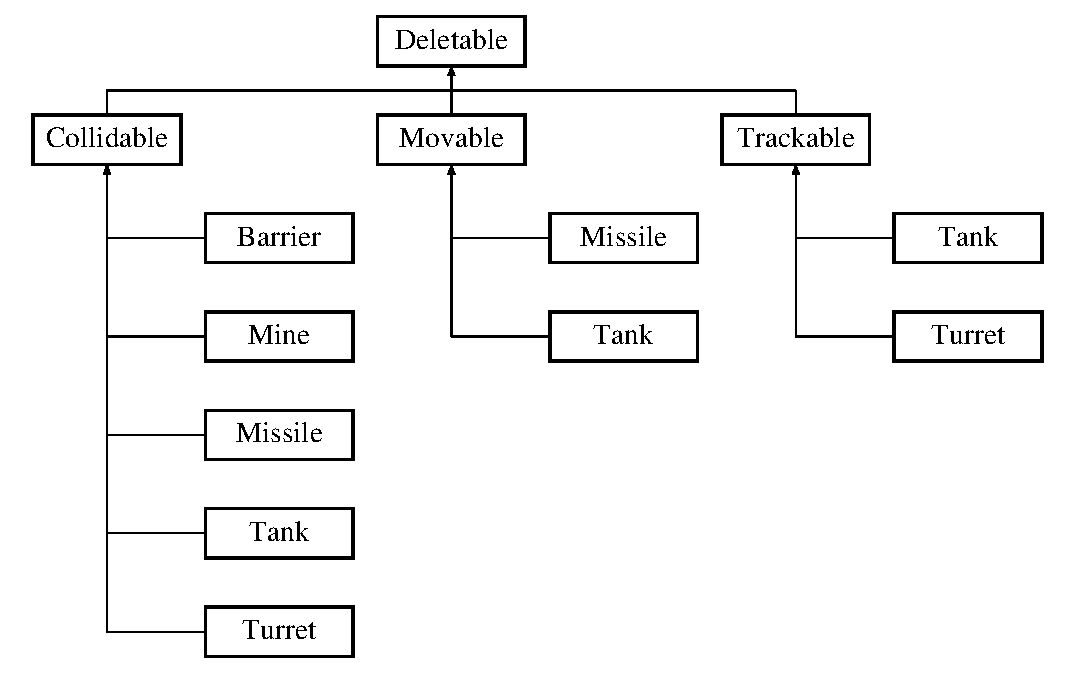
\includegraphics[height=7.000000cm]{classDeletable}
\end{center}
\end{figure}
\subsection*{Public Member Functions}
\begin{DoxyCompactItemize}
\item 
\hyperlink{classDeletable_a0ffa30c5232f87be98552a0dc90ab4ef}{Deletable} ()
\begin{DoxyCompactList}\small\item\em Constructor. \end{DoxyCompactList}\item 
virtual const bool \hyperlink{classDeletable_a6572440c291077cf52bf21288c6cd25c}{is\-Deleted} ()=0
\begin{DoxyCompactList}\small\item\em Check the death state of an entity. \end{DoxyCompactList}\item 
virtual const \hyperlink{Structures_8h_a6d8f83e710b27d4f86c45f0bb77066e3}{entity\-\_\-type} \& \hyperlink{classDeletable_af8a0208abc297180873692f4215fe50f}{get\-Type} () const =0
\begin{DoxyCompactList}\small\item\em Recieve the identification of the created object. \end{DoxyCompactList}\item 
virtual const float \hyperlink{classDeletable_ac14ea0c5986d50ba3ba454f89c87b8fe}{get\-Draw\-Position\-X} ()=0
\begin{DoxyCompactList}\small\item\em Retrieve the entity's x Position. \end{DoxyCompactList}\item 
virtual const float \hyperlink{classDeletable_a2a88d7e40c56902a3d3d8f668e9d126d}{get\-Draw\-Position\-Y} ()=0
\begin{DoxyCompactList}\small\item\em Retrieve the entity's y Position. \end{DoxyCompactList}\item 
virtual const float \hyperlink{classDeletable_ad7061a6bef3efce030aa5abbc7646d47}{get\-Draw\-Rotation} ()=0
\begin{DoxyCompactList}\small\item\em Retrieve the entity's Position. \end{DoxyCompactList}\item 
virtual \hyperlink{classDeletable_a20633231281c5a7110389a3f416f4989}{$\sim$\-Deletable} ()=0
\begin{DoxyCompactList}\small\item\em Destructor. \end{DoxyCompactList}\end{DoxyCompactItemize}


\subsection{Detailed Description}


Definition at line 19 of file Deletable.\-h.



\subsection{Constructor \& Destructor Documentation}
\hypertarget{classDeletable_a0ffa30c5232f87be98552a0dc90ab4ef}{\index{Deletable@{Deletable}!Deletable@{Deletable}}
\index{Deletable@{Deletable}!Deletable@{Deletable}}
\subsubsection[{Deletable}]{\setlength{\rightskip}{0pt plus 5cm}Deletable\-::\-Deletable (
\begin{DoxyParamCaption}
{}
\end{DoxyParamCaption}
)}}\label{classDeletable_a0ffa30c5232f87be98552a0dc90ab4ef}


Constructor. 



Definition at line 12 of file Deletable.\-cpp.


\begin{DoxyCode}
13 \{
14 
15 \}
\end{DoxyCode}
\hypertarget{classDeletable_a20633231281c5a7110389a3f416f4989}{\index{Deletable@{Deletable}!$\sim$\-Deletable@{$\sim$\-Deletable}}
\index{$\sim$\-Deletable@{$\sim$\-Deletable}!Deletable@{Deletable}}
\subsubsection[{$\sim$\-Deletable}]{\setlength{\rightskip}{0pt plus 5cm}Deletable\-::$\sim$\-Deletable (
\begin{DoxyParamCaption}
{}
\end{DoxyParamCaption}
)\hspace{0.3cm}{\ttfamily [pure virtual]}}}\label{classDeletable_a20633231281c5a7110389a3f416f4989}


Destructor. 



Definition at line 18 of file Deletable.\-cpp.


\begin{DoxyCode}
19 \{
20 
21 \}
\end{DoxyCode}


\subsection{Member Function Documentation}
\hypertarget{classDeletable_ac14ea0c5986d50ba3ba454f89c87b8fe}{\index{Deletable@{Deletable}!get\-Draw\-Position\-X@{get\-Draw\-Position\-X}}
\index{get\-Draw\-Position\-X@{get\-Draw\-Position\-X}!Deletable@{Deletable}}
\subsubsection[{get\-Draw\-Position\-X}]{\setlength{\rightskip}{0pt plus 5cm}virtual const float Deletable\-::get\-Draw\-Position\-X (
\begin{DoxyParamCaption}
{}
\end{DoxyParamCaption}
)\hspace{0.3cm}{\ttfamily [pure virtual]}}}\label{classDeletable_ac14ea0c5986d50ba3ba454f89c87b8fe}


Retrieve the entity's x Position. 



Implemented in \hyperlink{classTank_a679ab65e5d46ee6e7fa5fe517101131f}{Tank}, \hyperlink{classMissile_a8e8d526d7578cfbabbd5bf1bdb9727bc}{Missile}, \hyperlink{classBarrier_a53317aaef27996362c933d65914d663c}{Barrier}, \hyperlink{classMine_a904342dcd8d13f8489c91ed6ba09ec7b}{Mine}, and \hyperlink{classTurret_aecf0bc7d827c8f05f48b730daf00d9e4}{Turret}.

\hypertarget{classDeletable_a2a88d7e40c56902a3d3d8f668e9d126d}{\index{Deletable@{Deletable}!get\-Draw\-Position\-Y@{get\-Draw\-Position\-Y}}
\index{get\-Draw\-Position\-Y@{get\-Draw\-Position\-Y}!Deletable@{Deletable}}
\subsubsection[{get\-Draw\-Position\-Y}]{\setlength{\rightskip}{0pt plus 5cm}virtual const float Deletable\-::get\-Draw\-Position\-Y (
\begin{DoxyParamCaption}
{}
\end{DoxyParamCaption}
)\hspace{0.3cm}{\ttfamily [pure virtual]}}}\label{classDeletable_a2a88d7e40c56902a3d3d8f668e9d126d}


Retrieve the entity's y Position. 



Implemented in \hyperlink{classTank_a5778b15fc49b6cd1086f3a80383b2a37}{Tank}, \hyperlink{classMissile_ad609bee2bfaf610824f32c15430fa6d8}{Missile}, \hyperlink{classBarrier_af90c9b4b6f28c7710637ccda7148fbd4}{Barrier}, \hyperlink{classMine_a8abe866b857f781f81b0b3b4e9ef7034}{Mine}, and \hyperlink{classTurret_ab86c156ea9ba76d33458601aa0eb454b}{Turret}.

\hypertarget{classDeletable_ad7061a6bef3efce030aa5abbc7646d47}{\index{Deletable@{Deletable}!get\-Draw\-Rotation@{get\-Draw\-Rotation}}
\index{get\-Draw\-Rotation@{get\-Draw\-Rotation}!Deletable@{Deletable}}
\subsubsection[{get\-Draw\-Rotation}]{\setlength{\rightskip}{0pt plus 5cm}virtual const float Deletable\-::get\-Draw\-Rotation (
\begin{DoxyParamCaption}
{}
\end{DoxyParamCaption}
)\hspace{0.3cm}{\ttfamily [pure virtual]}}}\label{classDeletable_ad7061a6bef3efce030aa5abbc7646d47}


Retrieve the entity's Position. 



Implemented in \hyperlink{classTank_aa117515fda912f25f9f7d5a8ce4055d7}{Tank}, \hyperlink{classMissile_ab606b0b4f38c821063f210625f926374}{Missile}, \hyperlink{classBarrier_aac579711db52df907e86ef4deea7ba1d}{Barrier}, \hyperlink{classMine_a5b6986a3a3ce5177879359a626cc994b}{Mine}, and \hyperlink{classTurret_a52a79fd86533f6b3d94223a60df41aaa}{Turret}.

\hypertarget{classDeletable_af8a0208abc297180873692f4215fe50f}{\index{Deletable@{Deletable}!get\-Type@{get\-Type}}
\index{get\-Type@{get\-Type}!Deletable@{Deletable}}
\subsubsection[{get\-Type}]{\setlength{\rightskip}{0pt plus 5cm}virtual const {\bf entity\-\_\-type}\& Deletable\-::get\-Type (
\begin{DoxyParamCaption}
{}
\end{DoxyParamCaption}
) const\hspace{0.3cm}{\ttfamily [pure virtual]}}}\label{classDeletable_af8a0208abc297180873692f4215fe50f}


Recieve the identification of the created object. 



Implemented in \hyperlink{classTank_a13af6c47c61682ebd1463fd9ef34439b}{Tank}, \hyperlink{classMissile_a67874a53d50f63065bf1f63803558513}{Missile}, \hyperlink{classBarrier_a649b80eadc6948e68947f7516fee258c}{Barrier}, \hyperlink{classTurret_a4998bf256706dc75926e683f08862b80}{Turret}, and \hyperlink{classMine_af435cf100fe7f89e998ec2f7ad40faa1}{Mine}.

\hypertarget{classDeletable_a6572440c291077cf52bf21288c6cd25c}{\index{Deletable@{Deletable}!is\-Deleted@{is\-Deleted}}
\index{is\-Deleted@{is\-Deleted}!Deletable@{Deletable}}
\subsubsection[{is\-Deleted}]{\setlength{\rightskip}{0pt plus 5cm}virtual const bool Deletable\-::is\-Deleted (
\begin{DoxyParamCaption}
{}
\end{DoxyParamCaption}
)\hspace{0.3cm}{\ttfamily [pure virtual]}}}\label{classDeletable_a6572440c291077cf52bf21288c6cd25c}


Check the death state of an entity. 



Implemented in \hyperlink{classTank_a33a62b283cdaf362415fad768d2f6df3}{Tank}, \hyperlink{classMissile_a96c1240f08fed605ff9e908a0bea50e4}{Missile}, \hyperlink{classBarrier_a8199ad8a6f070435da55832bdd3893b8}{Barrier}, \hyperlink{classMine_aa19d1827e837944d74fe02ad0fbeffc9}{Mine}, and \hyperlink{classTurret_a204a0c45ddcc9139cda14dcd1493fd86}{Turret}.



The documentation for this class was generated from the following files\-:\begin{DoxyCompactItemize}
\item 
\hyperlink{Deletable_8h}{Deletable.\-h}\item 
\hyperlink{Deletable_8cpp}{Deletable.\-cpp}\end{DoxyCompactItemize}

\hypertarget{classDestructionManager}{\section{Destruction\-Manager Class Reference}
\label{classDestructionManager}\index{Destruction\-Manager@{Destruction\-Manager}}
}


\hyperlink{classManager}{Manager} class responsible for deletions of destroyed game entities.  




{\ttfamily \#include $<$Destruction\-Manager.\-h$>$}

Inheritance diagram for Destruction\-Manager\-:\begin{figure}[H]
\begin{center}
\leavevmode
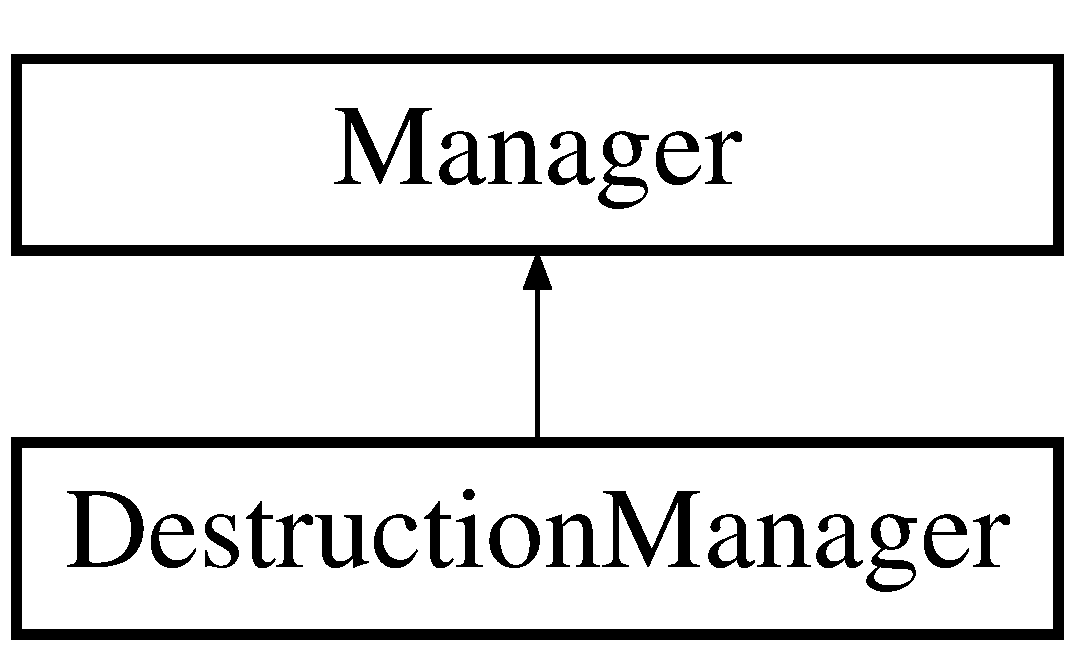
\includegraphics[height=2.000000cm]{classDestructionManager}
\end{center}
\end{figure}
\subsection*{Public Member Functions}
\begin{DoxyCompactItemize}
\item 
\hyperlink{classDestructionManager_aec752aef0eb6b659293910c011e0fe93}{Destruction\-Manager} ()
\begin{DoxyCompactList}\small\item\em Constructor for the Destruction manager. \end{DoxyCompactList}\item 
void \hyperlink{classDestructionManager_acfb0e5bf3e2d24368918b4246a972394}{manage} (\hyperlink{classGameStateData}{Game\-State\-Data} \&game\-\_\-state\-\_\-container)
\begin{DoxyCompactList}\small\item\em Destruction management process for the Destruction \hyperlink{classManager}{Manager}. \end{DoxyCompactList}\item 
void \hyperlink{classDestructionManager_a666b4ad3ae0c1383e4c9f53a48daf2ce}{add\-New\-Entity} (std\-::shared\-\_\-ptr$<$ \hyperlink{classDeletable}{Deletable} $>$ new\-\_\-entity)
\begin{DoxyCompactList}\small\item\em Add Deletable-\/type shared\-\_\-ptr's to the Destruction\-Managers internal data members. \end{DoxyCompactList}\item 
virtual \hyperlink{classDestructionManager_a0c43cc0724e29a707e5a190c7f0d6761}{$\sim$\-Destruction\-Manager} ()
\begin{DoxyCompactList}\small\item\em Destructor for the destruction manager. \end{DoxyCompactList}\end{DoxyCompactItemize}
\subsection*{Private Attributes}
\begin{DoxyCompactItemize}
\item 
std\-::vector$<$ std\-::shared\-\_\-ptr\\*
$<$ \hyperlink{classDeletable}{Deletable} $>$ $>$ \hyperlink{classDestructionManager_a4abb9d43e2508c82519e0fedde734670}{\-\_\-destructables}
\end{DoxyCompactItemize}


\subsection{Detailed Description}
\hyperlink{classManager}{Manager} class responsible for deletions of destroyed game entities. 

Definition at line 21 of file Destruction\-Manager.\-h.



\subsection{Constructor \& Destructor Documentation}
\hypertarget{classDestructionManager_aec752aef0eb6b659293910c011e0fe93}{\index{Destruction\-Manager@{Destruction\-Manager}!Destruction\-Manager@{Destruction\-Manager}}
\index{Destruction\-Manager@{Destruction\-Manager}!DestructionManager@{Destruction\-Manager}}
\subsubsection[{Destruction\-Manager}]{\setlength{\rightskip}{0pt plus 5cm}Destruction\-Manager\-::\-Destruction\-Manager (
\begin{DoxyParamCaption}
{}
\end{DoxyParamCaption}
)}}\label{classDestructionManager_aec752aef0eb6b659293910c011e0fe93}


Constructor for the Destruction manager. 



Definition at line 13 of file Destruction\-Manager.\-cpp.


\begin{DoxyCode}
14  \{
15 
16  \}
\end{DoxyCode}
\hypertarget{classDestructionManager_a0c43cc0724e29a707e5a190c7f0d6761}{\index{Destruction\-Manager@{Destruction\-Manager}!$\sim$\-Destruction\-Manager@{$\sim$\-Destruction\-Manager}}
\index{$\sim$\-Destruction\-Manager@{$\sim$\-Destruction\-Manager}!DestructionManager@{Destruction\-Manager}}
\subsubsection[{$\sim$\-Destruction\-Manager}]{\setlength{\rightskip}{0pt plus 5cm}Destruction\-Manager\-::$\sim$\-Destruction\-Manager (
\begin{DoxyParamCaption}
{}
\end{DoxyParamCaption}
)\hspace{0.3cm}{\ttfamily [virtual]}}}\label{classDestructionManager_a0c43cc0724e29a707e5a190c7f0d6761}


Destructor for the destruction manager. 



Definition at line 52 of file Destruction\-Manager.\-cpp.


\begin{DoxyCode}
53 \{
54     \textcolor{comment}{//Possible arguments to be added here}
55 \}
\end{DoxyCode}


\subsection{Member Function Documentation}
\hypertarget{classDestructionManager_a666b4ad3ae0c1383e4c9f53a48daf2ce}{\index{Destruction\-Manager@{Destruction\-Manager}!add\-New\-Entity@{add\-New\-Entity}}
\index{add\-New\-Entity@{add\-New\-Entity}!DestructionManager@{Destruction\-Manager}}
\subsubsection[{add\-New\-Entity}]{\setlength{\rightskip}{0pt plus 5cm}void Destruction\-Manager\-::add\-New\-Entity (
\begin{DoxyParamCaption}
\item[{std\-::shared\-\_\-ptr$<$ {\bf Deletable} $>$}]{new\-\_\-entity}
\end{DoxyParamCaption}
)}}\label{classDestructionManager_a666b4ad3ae0c1383e4c9f53a48daf2ce}


Add Deletable-\/type shared\-\_\-ptr's to the Destruction\-Managers internal data members. 


\begin{DoxyParams}{Parameters}
{\em new\-\_\-entity} & \-:\-: type of new entity that will be addded. \\
\hline
\end{DoxyParams}


Definition at line 60 of file Destruction\-Manager.\-cpp.



References \-\_\-destructables.



Referenced by Game\-::add\-New\-Mine(), Game\-::add\-New\-Missile(), Game\-::add\-New\-Tank(), Game\-::add\-New\-Turret(), Game\-::create\-Barrier(), main(), and T\-E\-S\-T().


\begin{DoxyCode}
61 \{
62     \hyperlink{classDestructionManager_a4abb9d43e2508c82519e0fedde734670}{\_destructables}.push\_back(new\_entity);
63 \}
\end{DoxyCode}
\hypertarget{classDestructionManager_acfb0e5bf3e2d24368918b4246a972394}{\index{Destruction\-Manager@{Destruction\-Manager}!manage@{manage}}
\index{manage@{manage}!DestructionManager@{Destruction\-Manager}}
\subsubsection[{manage}]{\setlength{\rightskip}{0pt plus 5cm}void Destruction\-Manager\-::manage (
\begin{DoxyParamCaption}
\item[{{\bf Game\-State\-Data} \&}]{game\-\_\-state\-\_\-container}
\end{DoxyParamCaption}
)}}\label{classDestructionManager_acfb0e5bf3e2d24368918b4246a972394}


Destruction management process for the Destruction \hyperlink{classManager}{Manager}. 

If one of the tanks are destroyed, then opposing player receives an additional point. 
\begin{DoxyParams}{Parameters}
{\em game\-\_\-state\-\_\-container} & \-:\-: cotainer that holds the players' score \\
\hline
\end{DoxyParams}


Definition at line 22 of file Destruction\-Manager.\-cpp.



References \-\_\-destructables, Game\-State\-Data\-::increase\-P1\-Score(), Game\-State\-Data\-::increase\-P2\-Score(), p1\-\_\-tank, and p2\-\_\-tank.



Referenced by main(), Game\-::run\-All\-Managers(), and T\-E\-S\-T().


\begin{DoxyCode}
23 \{
24     \textcolor{keyword}{auto} i = \hyperlink{classDestructionManager_a4abb9d43e2508c82519e0fedde734670}{\_destructables}.begin();
25     \textcolor{keywordflow}{for}(; i != \hyperlink{classDestructionManager_a4abb9d43e2508c82519e0fedde734670}{\_destructables}.end();)
26     \{
27             std::shared\_ptr<Deletable> entity\_sp = (*i);
28 
29             \textcolor{comment}{//The manager checks each entity to see if it has recieved a 'death state'}
30             \textcolor{keywordflow}{if}(entity\_sp->isDeleted())
31             \{
32                 \textcolor{keywordflow}{if} (entity\_sp->getType() == \hyperlink{Structures_8h_a6d8f83e710b27d4f86c45f0bb77066e3a31fa78b2b7dd774f5158a16ef230932e}{p1\_tank})
33                 \{
34                     game\_state\_container.\hyperlink{classGameStateData_a28ec2cf2d7dd89bab394b611a83e7d4c}{increaseP1Score}();
35                 \}
36 
37                 \textcolor{keywordflow}{if} (entity\_sp->getType() == \hyperlink{Structures_8h_a6d8f83e710b27d4f86c45f0bb77066e3a3d48d62c7b88e7ee171698fe56dc9e59}{p2\_tank})
38                 \{
39                     game\_state\_container.\hyperlink{classGameStateData_a8b2470bafedd2c51cdc32199ae004b13}{increaseP2Score}();
40                 \}
41 
42                 \hyperlink{classDestructionManager_a4abb9d43e2508c82519e0fedde734670}{\_destructables}.erase(i);
43             \}
44             \textcolor{keywordflow}{else}
45             \{
46                 i++;
47             \}
48     \}
49 \}
\end{DoxyCode}


\subsection{Member Data Documentation}
\hypertarget{classDestructionManager_a4abb9d43e2508c82519e0fedde734670}{\index{Destruction\-Manager@{Destruction\-Manager}!\-\_\-destructables@{\-\_\-destructables}}
\index{\-\_\-destructables@{\-\_\-destructables}!DestructionManager@{Destruction\-Manager}}
\subsubsection[{\-\_\-destructables}]{\setlength{\rightskip}{0pt plus 5cm}std\-::vector$<$std\-::shared\-\_\-ptr$<${\bf Deletable}$>$ $>$ Destruction\-Manager\-::\-\_\-destructables\hspace{0.3cm}{\ttfamily [private]}}}\label{classDestructionManager_a4abb9d43e2508c82519e0fedde734670}


Definition at line 31 of file Destruction\-Manager.\-h.



Referenced by add\-New\-Entity(), and manage().



The documentation for this class was generated from the following files\-:\begin{DoxyCompactItemize}
\item 
\hyperlink{DestructionManager_8h}{Destruction\-Manager.\-h}\item 
\hyperlink{DestructionManager_8cpp}{Destruction\-Manager.\-cpp}\end{DoxyCompactItemize}

\hypertarget{classDisplay}{\section{Display Class Reference}
\label{classDisplay}\index{Display@{Display}}
}


Handles all draw and display functionality.  




{\ttfamily \#include $<$Display.\-h$>$}

\subsection*{Public Member Functions}
\begin{DoxyCompactItemize}
\item 
\hyperlink{classDisplay_a305a7d8fc20a838a73d5706820935136}{Display} (int window\-\_\-width=800, int window\-\_\-height=600)
\begin{DoxyCompactList}\small\item\em Constructor for \hyperlink{classDisplay}{Display} object. \end{DoxyCompactList}\item 
bool \hyperlink{classDisplay_abfcf2f222f42edcfa2c9b3949817ec84}{is\-Open} ()
\begin{DoxyCompactList}\small\item\em Checks if the game window is still open. \end{DoxyCompactList}\item 
void \hyperlink{classDisplay_aa56b082e14b61988f2d0d01617e0c27d}{poll\-Events} ()
\begin{DoxyCompactList}\small\item\em Checks S\-F\-M\-L window events. \end{DoxyCompactList}\item 
void \hyperlink{classDisplay_a14242933dd00fc1d50f9ae70d5121d14}{clear} ()
\begin{DoxyCompactList}\small\item\em Clears the display window. \end{DoxyCompactList}\item 
void \hyperlink{classDisplay_a2db7dc6b0ffa4851cf49f3d37095d185}{draw\-Background} ()
\begin{DoxyCompactList}\small\item\em Checks S\-F\-M\-L window events. \end{DoxyCompactList}\item 
void \hyperlink{classDisplay_a8eff4790fce1c95ad443b224c313488a}{draw\-Entity} (const \hyperlink{Structures_8h_a6d8f83e710b27d4f86c45f0bb77066e3}{entity\-\_\-type} \&entity, const \hyperlink{structsprite__draw__info}{sprite\-\_\-draw\-\_\-info} \&draw\-\_\-info)
\begin{DoxyCompactList}\small\item\em Draws a game entity. \end{DoxyCompactList}\item 
void \hyperlink{classDisplay_a37aef4a33faf48a6f0c777290f5334ce}{draw\-Text} (const \hyperlink{structdraw__strings}{draw\-\_\-strings} \&strings)
\begin{DoxyCompactList}\small\item\em Draws all text. \end{DoxyCompactList}\item 
void \hyperlink{classDisplay_afe5f3569e0746afdb6d3f82fadc123a9}{draw\-End\-Screen} ()
\begin{DoxyCompactList}\small\item\em Draws the end game screen. \end{DoxyCompactList}\item 
void \hyperlink{classDisplay_aa3ab70ec7b76fa3ed139d19e53e72283}{display} ()
\begin{DoxyCompactList}\small\item\em Displays what has been drawn. \end{DoxyCompactList}\end{DoxyCompactItemize}
\subsection*{Private Member Functions}
\begin{DoxyCompactItemize}
\item 
void \hyperlink{classDisplay_a5af58e6a5eea9fcf573d2554891de781}{load\-Textures} ()
\begin{DoxyCompactList}\small\item\em Loads all textures as Rectangles. \end{DoxyCompactList}\item 
void \hyperlink{classDisplay_a410deedeb944684de238030348d3feab}{add\-Sprites} ()
\begin{DoxyCompactList}\small\item\em All pointers to S\-F\-M\-L sprites are made here. \end{DoxyCompactList}\item 
void \hyperlink{classDisplay_ad831893d7d3656e456c7f5c6915701f1}{setup\-Text} (sf\-::\-Text \&text)
\begin{DoxyCompactList}\small\item\em Initialises font properties. \end{DoxyCompactList}\end{DoxyCompactItemize}
\subsection*{Private Attributes}
\begin{DoxyCompactItemize}
\item 
int \hyperlink{classDisplay_a715bf4b76abf3b8a8cc495cbb7dfd4b0}{\-\_\-window\-\_\-width}
\begin{DoxyCompactList}\small\item\em \hyperlink{classDisplay}{Display} window width. \end{DoxyCompactList}\item 
int \hyperlink{classDisplay_a3e66e647786a79f49b985d45e1ad4ac2}{\-\_\-window\-\_\-height}
\begin{DoxyCompactList}\small\item\em \hyperlink{classDisplay}{Display} window height. \end{DoxyCompactList}\item 
sf\-::\-Render\-Window \hyperlink{classDisplay_aeb0bd9ad8ee786de5f4f0f7c738b1b11}{\-\_\-window}
\begin{DoxyCompactList}\small\item\em S\-F\-M\-L window where all sprites are drawn. \end{DoxyCompactList}\item 
\hyperlink{classSpriteDimensions}{Sprite\-Dimensions} \hyperlink{classDisplay_acf0a20ec8a01c1917d62f20ddf2d2f51}{\-\_\-game\-\_\-sprite\-\_\-dimensions}
\begin{DoxyCompactList}\small\item\em Holds information about all the sprite dimensions. \end{DoxyCompactList}\item 
\hyperlink{structtextures}{textures} \hyperlink{classDisplay_a64ae525710346f1a982efa05b8c53a88}{\-\_\-game\-\_\-textures}
\begin{DoxyCompactList}\small\item\em Struct of all textures in the game. \end{DoxyCompactList}\item 
const std\-::string \hyperlink{classDisplay_a4055ddd33815347b986bb7437bdc1c79}{\-\_\-tank1\-\_\-texture\-\_\-file} = \char`\"{}tank\-\_\-blue.\-png\char`\"{}
\begin{DoxyCompactList}\small\item\em \hyperlink{classTank}{Tank} 1 texture file name. \end{DoxyCompactList}\item 
const std\-::string \hyperlink{classDisplay_a5ab9e2102af414ee9d1d8d5b090ad9da}{\-\_\-tank2\-\_\-texture\-\_\-file} = \char`\"{}tank\-\_\-red.\-png\char`\"{}
\begin{DoxyCompactList}\small\item\em \hyperlink{classTank}{Tank} 2 texture file name. \end{DoxyCompactList}\item 
const std\-::string \hyperlink{classDisplay_a11a966967d1bfa745d910f25da35b6fb}{\-\_\-missile\-\_\-texture\-\_\-file} = \char`\"{}missile.\-png\char`\"{}
\begin{DoxyCompactList}\small\item\em Tanks missile texture file name. \end{DoxyCompactList}\item 
const std\-::string \hyperlink{classDisplay_a9b6a965f2d1ca97d9c243d4bbd941994}{\-\_\-mine\-\_\-texture\-\_\-file} = \char`\"{}mine.\-png\char`\"{}
\begin{DoxyCompactList}\small\item\em \hyperlink{classMine}{Mine} texture file name. \end{DoxyCompactList}\item 
const std\-::string \hyperlink{classDisplay_af921ed4131e5d5763e76ea7c54c3fea8}{\-\_\-barrier\-\_\-texture\-\_\-file} = \char`\"{}barrier.\-png\char`\"{}
\begin{DoxyCompactList}\small\item\em \hyperlink{classBarrier}{Barrier} texture file name. \end{DoxyCompactList}\item 
const std\-::string \hyperlink{classDisplay_a1e2dc0b7ef570f4584b7f171330a209d}{\-\_\-turret\-\_\-texture\-\_\-file} = \char`\"{}turret.\-png\char`\"{}
\begin{DoxyCompactList}\small\item\em \hyperlink{classTurret}{Turret} texture file name. \end{DoxyCompactList}\item 
const std\-::string \hyperlink{classDisplay_ac3bdb11a00913038ceeee3171fa99ea3}{\-\_\-map\-\_\-texture\-\_\-file} = \char`\"{}map.\-png\char`\"{}
\begin{DoxyCompactList}\small\item\em Map (background) texture file name. \end{DoxyCompactList}\item 
const std\-::string \hyperlink{classDisplay_a4d984df72ac348f13c50357bc58ad797}{\-\_\-missile\-\_\-turret\-\_\-texture\-\_\-file} = \char`\"{}missile\-\_\-turret.\-png\char`\"{}
\begin{DoxyCompactList}\small\item\em \hyperlink{classTurret}{Turret} missile texture file name. \end{DoxyCompactList}\item 
const std\-::string \hyperlink{classDisplay_a69effabf34c7f71ddf83be77977b56f2}{\-\_\-font\-\_\-file} = \char`\"{}futura\-\_\-light.\-ttf\char`\"{}
\begin{DoxyCompactList}\small\item\em Font file name. \end{DoxyCompactList}\item 
const std\-::string \hyperlink{classDisplay_ac8eb9dbc23ed61c56ea69adfdbfeecde}{\-\_\-end\-\_\-texture\-\_\-file} = \char`\"{}end\-\_\-screen.\-png\char`\"{}
\begin{DoxyCompactList}\small\item\em End screen texture file name. \end{DoxyCompactList}\item 
std\-::map$<$ \hyperlink{Structures_8h_a6d8f83e710b27d4f86c45f0bb77066e3}{entity\-\_\-type}, \\*
std\-::shared\-\_\-ptr$<$ sf\-::\-Sprite $>$ $>$ \hyperlink{classDisplay_a975326ca007706c154317ddef67000f4}{\-\_\-sprites}
\begin{DoxyCompactList}\small\item\em Map container for the sprites that will be drawn. \end{DoxyCompactList}\item 
sf\-::\-Sprite \hyperlink{classDisplay_a2ec82cf1355d968c3863c9089ab2e511}{\-\_\-map\-\_\-sprite}
\begin{DoxyCompactList}\small\item\em Map (background) S\-F\-M\-L sprite. \end{DoxyCompactList}\item 
sf\-::\-Sprite \hyperlink{classDisplay_a3bcec98cfc7e32f4fb46e625d76984a0}{\-\_\-end\-\_\-map\-\_\-sprite}
\begin{DoxyCompactList}\small\item\em End game screen sprite. \end{DoxyCompactList}\item 
sf\-::\-Texture \hyperlink{classDisplay_aa98ca168c20ac56fe56def6686cf9f91}{\-\_\-map\-\_\-texture}
\begin{DoxyCompactList}\small\item\em Map (background) S\-F\-M\-L texture. \end{DoxyCompactList}\item 
sf\-::\-Texture \hyperlink{classDisplay_ad41d7097510e56a9f16e97d7cc13c5b6}{\-\_\-end\-\_\-map\-\_\-texture}
\begin{DoxyCompactList}\small\item\em End game screen texture. \end{DoxyCompactList}\item 
sf\-::\-Text \hyperlink{classDisplay_a36007f3ed0cb7f8174ef601dbde3adab}{\-\_\-game\-\_\-time\-\_\-text}
\begin{DoxyCompactList}\small\item\em Runtime S\-F\-M\-L text. \end{DoxyCompactList}\item 
sf\-::\-Text \hyperlink{classDisplay_a0545991d352f9d4e7bda7d2f3b6a0236}{\-\_\-p1\-\_\-score\-\_\-text}
\begin{DoxyCompactList}\small\item\em Player 1 S\-F\-M\-L score text. \end{DoxyCompactList}\item 
sf\-::\-Text \hyperlink{classDisplay_a80ea7a2642db4a379d756b0132d26343}{\-\_\-p2\-\_\-score\-\_\-text}
\begin{DoxyCompactList}\small\item\em Player 2 S\-F\-M\-L score text. \end{DoxyCompactList}\item 
sf\-::\-Font \hyperlink{classDisplay_a937e4b846d090d1d520e15d6233bbfc0}{\-\_\-font\-\_\-style}
\begin{DoxyCompactList}\small\item\em S\-F\-M\-L font style. \end{DoxyCompactList}\item 
const int \hyperlink{classDisplay_ae10066fc5854e77ea65d3a64912b079a}{\-\_\-font\-\_\-size} = 20
\begin{DoxyCompactList}\small\item\em Constant size for all window fonts. \end{DoxyCompactList}\item 
const int \hyperlink{classDisplay_ae85ee765b92689445aca8cead24d8184}{\-\_\-text\-\_\-y\-\_\-allignment} = 0
\begin{DoxyCompactList}\small\item\em Vertical alignment for runtime and player scores. \end{DoxyCompactList}\item 
const int \hyperlink{classDisplay_ad9b50fa7903081469111841965b995ba}{\-\_\-game\-\_\-time\-\_\-pos} = 550
\begin{DoxyCompactList}\small\item\em Horzontal position of game time text. \end{DoxyCompactList}\item 
const int \hyperlink{classDisplay_af7115b9c3e4cdedf1398bcbdbf794270}{\-\_\-p1\-\_\-score\-\_\-pos} = 950
\begin{DoxyCompactList}\small\item\em Horizontal position of player 1 score text. \end{DoxyCompactList}\item 
const int \hyperlink{classDisplay_a223efbfb6036d823dbaf09e4180a07fb}{\-\_\-p2\-\_\-score\-\_\-pos} = 100
\begin{DoxyCompactList}\small\item\em Horizontal position of player 2 score text. \end{DoxyCompactList}\end{DoxyCompactItemize}


\subsection{Detailed Description}
Handles all draw and display functionality. 

Definition at line 20 of file Display.\-h.



\subsection{Constructor \& Destructor Documentation}
\hypertarget{classDisplay_a305a7d8fc20a838a73d5706820935136}{\index{Display@{Display}!Display@{Display}}
\index{Display@{Display}!Display@{Display}}
\subsubsection[{Display}]{\setlength{\rightskip}{0pt plus 5cm}Display\-::\-Display (
\begin{DoxyParamCaption}
\item[{int}]{window\-\_\-width = {\ttfamily 800}, }
\item[{int}]{window\-\_\-height = {\ttfamily 600}}
\end{DoxyParamCaption}
)}}\label{classDisplay_a305a7d8fc20a838a73d5706820935136}


Constructor for \hyperlink{classDisplay}{Display} object. 

Initialises window dimensions as well as other private objects. The game window title can be changed within the \-\_\-window constructor. The rest of the function makes sure that the main map textures are loaded correctly. The text objects for the game are also initialised here. 
\begin{DoxyParams}{Parameters}
{\em window\-\_\-width} & \-:\-: default is set to 800 \\
\hline
{\em window\-\_\-height} & \-:\-: default is set to 600 \\
\hline
\end{DoxyParams}


Definition at line 26 of file Display.\-cpp.



References \-\_\-end\-\_\-map\-\_\-sprite, \-\_\-end\-\_\-map\-\_\-texture, \-\_\-end\-\_\-texture\-\_\-file, \-\_\-font\-\_\-file, \-\_\-font\-\_\-style, \-\_\-game\-\_\-time\-\_\-pos, \-\_\-game\-\_\-time\-\_\-text, \-\_\-map\-\_\-sprite, \-\_\-map\-\_\-texture, \-\_\-map\-\_\-texture\-\_\-file, \-\_\-p1\-\_\-score\-\_\-pos, \-\_\-p1\-\_\-score\-\_\-text, \-\_\-p2\-\_\-score\-\_\-pos, \-\_\-p2\-\_\-score\-\_\-text, \-\_\-text\-\_\-y\-\_\-allignment, \-\_\-window, add\-Sprites(), load\-Textures(), and setup\-Text().


\begin{DoxyCode}
26                                                    :
27     \hyperlink{classDisplay_a715bf4b76abf3b8a8cc495cbb7dfd4b0}{\_window\_width}(window\_width),
28     \hyperlink{classDisplay_a3e66e647786a79f49b985d45e1ad4ac2}{\_window\_height}(window\_height),
29     \hyperlink{classDisplay_aeb0bd9ad8ee786de5f4f0f7c738b1b11}{\_window}(sf::VideoMode(\hyperlink{classDisplay_a715bf4b76abf3b8a8cc495cbb7dfd4b0}{\_window\_width},\hyperlink{classDisplay_a3e66e647786a79f49b985d45e1ad4ac2}{\_window\_height}), \textcolor{stringliteral}{"Tank A Lot"}),
30     \hyperlink{classDisplay_a64ae525710346f1a982efa05b8c53a88}{\_game\_textures}(),
31     \hyperlink{classDisplay_acf0a20ec8a01c1917d62f20ddf2d2f51}{\_game\_sprite\_dimensions}()
32 \{
33     \hyperlink{classDisplay_a5af58e6a5eea9fcf573d2554891de781}{loadTextures}();
34     \hyperlink{classDisplay_a410deedeb944684de238030348d3feab}{addSprites}();
35 
36     \textcolor{keywordflow}{if} (!\hyperlink{classDisplay_aa98ca168c20ac56fe56def6686cf9f91}{\_map\_texture}.loadFromFile(\hyperlink{classDisplay_ac3bdb11a00913038ceeee3171fa99ea3}{\_map\_texture\_file}))
37         std::cout << \textcolor{stringliteral}{"Unable to load Map file!"} << std::endl;
38 
39     \hyperlink{classDisplay_a2ec82cf1355d968c3863c9089ab2e511}{\_map\_sprite}.setTexture(\hyperlink{classDisplay_aa98ca168c20ac56fe56def6686cf9f91}{\_map\_texture});
40 
41     \textcolor{keywordflow}{if} (!\hyperlink{classDisplay_ad41d7097510e56a9f16e97d7cc13c5b6}{\_end\_map\_texture}.loadFromFile(\hyperlink{classDisplay_ac8eb9dbc23ed61c56ea69adfdbfeecde}{\_end\_texture\_file}))
42         std::cout << \textcolor{stringliteral}{"Unable to load Map file!"} << std::endl;
43 
44     \hyperlink{classDisplay_a3bcec98cfc7e32f4fb46e625d76984a0}{\_end\_map\_sprite}.setTexture(\hyperlink{classDisplay_ad41d7097510e56a9f16e97d7cc13c5b6}{\_end\_map\_texture});
45 
46     \textcolor{keywordflow}{if} (!\hyperlink{classDisplay_a937e4b846d090d1d520e15d6233bbfc0}{\_font\_style}.loadFromFile(\hyperlink{classDisplay_a69effabf34c7f71ddf83be77977b56f2}{\_font\_file}))
47        std::cout << \textcolor{stringliteral}{"Unable to load font file!"} << std::endl;
48 
49     \hyperlink{classDisplay_ad831893d7d3656e456c7f5c6915701f1}{setupText}(\hyperlink{classDisplay_a36007f3ed0cb7f8174ef601dbde3adab}{\_game\_time\_text});
50     \hyperlink{classDisplay_a36007f3ed0cb7f8174ef601dbde3adab}{\_game\_time\_text}.setPosition(\hyperlink{classDisplay_ad9b50fa7903081469111841965b995ba}{\_game\_time\_pos},
      \hyperlink{classDisplay_ae85ee765b92689445aca8cead24d8184}{\_text\_y\_allignment});
51 
52     \hyperlink{classDisplay_ad831893d7d3656e456c7f5c6915701f1}{setupText}(\hyperlink{classDisplay_a0545991d352f9d4e7bda7d2f3b6a0236}{\_p1\_score\_text});
53     \hyperlink{classDisplay_a0545991d352f9d4e7bda7d2f3b6a0236}{\_p1\_score\_text}.setPosition(\hyperlink{classDisplay_af7115b9c3e4cdedf1398bcbdbf794270}{\_p1\_score\_pos},
      \hyperlink{classDisplay_ae85ee765b92689445aca8cead24d8184}{\_text\_y\_allignment});
54 
55     \hyperlink{classDisplay_ad831893d7d3656e456c7f5c6915701f1}{setupText}(\hyperlink{classDisplay_a80ea7a2642db4a379d756b0132d26343}{\_p2\_score\_text});
56     \hyperlink{classDisplay_a80ea7a2642db4a379d756b0132d26343}{\_p2\_score\_text}.setPosition(\hyperlink{classDisplay_a223efbfb6036d823dbaf09e4180a07fb}{\_p2\_score\_pos},
      \hyperlink{classDisplay_ae85ee765b92689445aca8cead24d8184}{\_text\_y\_allignment});
57 
58     \hyperlink{classDisplay_aeb0bd9ad8ee786de5f4f0f7c738b1b11}{\_window}.setFramerateLimit(60);
59 
60 \}
\end{DoxyCode}


\subsection{Member Function Documentation}
\hypertarget{classDisplay_a410deedeb944684de238030348d3feab}{\index{Display@{Display}!add\-Sprites@{add\-Sprites}}
\index{add\-Sprites@{add\-Sprites}!Display@{Display}}
\subsubsection[{add\-Sprites}]{\setlength{\rightskip}{0pt plus 5cm}void Display\-::add\-Sprites (
\begin{DoxyParamCaption}
{}
\end{DoxyParamCaption}
)\hspace{0.3cm}{\ttfamily [private]}}}\label{classDisplay_a410deedeb944684de238030348d3feab}


All pointers to S\-F\-M\-L sprites are made here. 

Each sprite is created and accessed via a shared\-\_\-ptr. They are saved in a map so that they can be referenced when drawn. This means that the number of sprites that exist are equal to the number of unique sprites. It is from this map that a copy of the sprite is drawn. Any new sprites that will be drawn can be added here. 

Definition at line 117 of file Display.\-cpp.



References \-\_\-game\-\_\-textures, \-\_\-sprites, barrier, textures\-::barrier, textures\-::mine, textures\-::missile, p1\-\_\-mine, p1\-\_\-missile, p1\-\_\-tank, p2\-\_\-mine, p2\-\_\-missile, p2\-\_\-tank, textures\-::tank\-\_\-1, textures\-::tank\-\_\-2, turret, textures\-::turret, turret\-\_\-missile, and textures\-::turret\-\_\-missile.



Referenced by Display().


\begin{DoxyCode}
118 \{
119     \textcolor{comment}{//Create P\_1 Tank Sprite}
120     std::shared\_ptr<sf::Sprite> tank1\_sp(\textcolor{keyword}{new}(sf::Sprite));
121     tank1\_sp->setTexture(\hyperlink{classDisplay_a64ae525710346f1a982efa05b8c53a88}{\_game\_textures}.\hyperlink{structtextures_a9287e247a5d108ed875b7b5b89ded524}{tank\_1});
122     \hyperlink{classDisplay_a975326ca007706c154317ddef67000f4}{\_sprites}.insert(std::pair<\hyperlink{Structures_8h_a6d8f83e710b27d4f86c45f0bb77066e3}{entity\_type}, std::shared\_ptr<sf::Sprite>>(
      \hyperlink{Structures_8h_a6d8f83e710b27d4f86c45f0bb77066e3a31fa78b2b7dd774f5158a16ef230932e}{p1\_tank},tank1\_sp));
123 
124     \textcolor{comment}{//Create P\_2 Tank Sprite}
125     std::shared\_ptr<sf::Sprite> tank2\_sp(\textcolor{keyword}{new}(sf::Sprite));
126     tank2\_sp->setTexture(\hyperlink{classDisplay_a64ae525710346f1a982efa05b8c53a88}{\_game\_textures}.\hyperlink{structtextures_a3322b3f064640afe1a4ebdb53636b71d}{tank\_2});
127     \hyperlink{classDisplay_a975326ca007706c154317ddef67000f4}{\_sprites}.insert(std::pair<\hyperlink{Structures_8h_a6d8f83e710b27d4f86c45f0bb77066e3}{entity\_type}, std::shared\_ptr<sf::Sprite>>(
      \hyperlink{Structures_8h_a6d8f83e710b27d4f86c45f0bb77066e3a3d48d62c7b88e7ee171698fe56dc9e59}{p2\_tank},tank2\_sp));
128 
129     \textcolor{comment}{//Create Barrier Sprite}
130     std::shared\_ptr<sf::Sprite> barrier\_sp(\textcolor{keyword}{new}(sf::Sprite));
131     barrier\_sp->setTexture(\hyperlink{classDisplay_a64ae525710346f1a982efa05b8c53a88}{\_game\_textures}.\hyperlink{structtextures_a36f35bd26858ecc8eb507e1072bfad7d}{barrier});
132     \hyperlink{classDisplay_a975326ca007706c154317ddef67000f4}{\_sprites}.insert(std::pair<\hyperlink{Structures_8h_a6d8f83e710b27d4f86c45f0bb77066e3}{entity\_type}, std::shared\_ptr<sf::Sprite>>(
      \hyperlink{Structures_8h_a6d8f83e710b27d4f86c45f0bb77066e3a6fb040c958f554e1d8320926b700b59d}{barrier},barrier\_sp));
133 
134     \textcolor{comment}{//Create P\_1 Missile Sprite}
135     std::shared\_ptr<sf::Sprite> missile1\_sp(\textcolor{keyword}{new}(sf::Sprite));
136     missile1\_sp->setTexture(\hyperlink{classDisplay_a64ae525710346f1a982efa05b8c53a88}{\_game\_textures}.\hyperlink{structtextures_a1d12557e92da80a9809f037edfe72f2f}{missile});
137     \hyperlink{classDisplay_a975326ca007706c154317ddef67000f4}{\_sprites}.insert(std::pair<\hyperlink{Structures_8h_a6d8f83e710b27d4f86c45f0bb77066e3}{entity\_type}, std::shared\_ptr<sf::Sprite>>(
      \hyperlink{Structures_8h_a6d8f83e710b27d4f86c45f0bb77066e3af89bc631e9b0140ed004b5ce2db5330c}{p1\_missile},missile1\_sp));
138 
139     \textcolor{comment}{//Create P\_2 Missile Sprite}
140     std::shared\_ptr<sf::Sprite> missile2\_sp(\textcolor{keyword}{new}(sf::Sprite));
141     missile2\_sp->setTexture(\hyperlink{classDisplay_a64ae525710346f1a982efa05b8c53a88}{\_game\_textures}.\hyperlink{structtextures_a1d12557e92da80a9809f037edfe72f2f}{missile});
142     \hyperlink{classDisplay_a975326ca007706c154317ddef67000f4}{\_sprites}.insert(std::pair<\hyperlink{Structures_8h_a6d8f83e710b27d4f86c45f0bb77066e3}{entity\_type}, std::shared\_ptr<sf::Sprite>>(
      \hyperlink{Structures_8h_a6d8f83e710b27d4f86c45f0bb77066e3a47100170e5852d632dfe65582a18256d}{p2\_missile},missile2\_sp));
143 
144     \textcolor{comment}{//Create P\_1 Mine Sprite}
145     std::shared\_ptr<sf::Sprite> mine1\_sp(\textcolor{keyword}{new}(sf::Sprite));
146     mine1\_sp->setTexture(\hyperlink{classDisplay_a64ae525710346f1a982efa05b8c53a88}{\_game\_textures}.\hyperlink{structtextures_a7f5b6643fd47d1bd8d5758c24c32dc9e}{mine});
147     \hyperlink{classDisplay_a975326ca007706c154317ddef67000f4}{\_sprites}.insert(std::pair<\hyperlink{Structures_8h_a6d8f83e710b27d4f86c45f0bb77066e3}{entity\_type}, std::shared\_ptr<sf::Sprite>>(
      \hyperlink{Structures_8h_a6d8f83e710b27d4f86c45f0bb77066e3afc52e626787e982ae5d0a747bed6666d}{p1\_mine},mine1\_sp));
148 
149     \textcolor{comment}{//Create P\_2 Mine Sprite}
150     std::shared\_ptr<sf::Sprite> mine2\_sp(\textcolor{keyword}{new}(sf::Sprite));
151     mine2\_sp->setTexture(\hyperlink{classDisplay_a64ae525710346f1a982efa05b8c53a88}{\_game\_textures}.\hyperlink{structtextures_a7f5b6643fd47d1bd8d5758c24c32dc9e}{mine});
152     \hyperlink{classDisplay_a975326ca007706c154317ddef67000f4}{\_sprites}.insert(std::pair<\hyperlink{Structures_8h_a6d8f83e710b27d4f86c45f0bb77066e3}{entity\_type}, std::shared\_ptr<sf::Sprite>>(
      \hyperlink{Structures_8h_a6d8f83e710b27d4f86c45f0bb77066e3ada293b37940e64ec2cf6dbd2ae493d2b}{p2\_mine},mine2\_sp));
153 
154     \textcolor{comment}{//Create Turret Sprite}
155     std::shared\_ptr<sf::Sprite> turret\_sp(\textcolor{keyword}{new}(sf::Sprite));
156     turret\_sp->setTexture(\hyperlink{classDisplay_a64ae525710346f1a982efa05b8c53a88}{\_game\_textures}.\hyperlink{structtextures_a8454a0f97657e68ca0076f19c4de6236}{turret});
157     \hyperlink{classDisplay_a975326ca007706c154317ddef67000f4}{\_sprites}.insert(std::pair<\hyperlink{Structures_8h_a6d8f83e710b27d4f86c45f0bb77066e3}{entity\_type}, std::shared\_ptr<sf::Sprite>>(
      \hyperlink{Structures_8h_a6d8f83e710b27d4f86c45f0bb77066e3a85c730ac9ffc13ac94e6e860579928a1}{turret},turret\_sp));
158 
159     \textcolor{comment}{//Create Turret Missile Sprite}
160     std::shared\_ptr<sf::Sprite> turret\_missile\_sp(\textcolor{keyword}{new}(sf::Sprite));
161     turret\_missile\_sp->setTexture(\hyperlink{classDisplay_a64ae525710346f1a982efa05b8c53a88}{\_game\_textures}.\hyperlink{structtextures_aa9ff61d80b32b3520308d8df61a8ea3f}{turret\_missile});
162     \hyperlink{classDisplay_a975326ca007706c154317ddef67000f4}{\_sprites}.insert(std::pair<\hyperlink{Structures_8h_a6d8f83e710b27d4f86c45f0bb77066e3}{entity\_type}, std::shared\_ptr<sf::Sprite>>(
      \hyperlink{Structures_8h_a6d8f83e710b27d4f86c45f0bb77066e3a8f552a1e495ced5aa8775faa1b6a757b}{turret\_missile},turret\_missile\_sp));
163 \}
\end{DoxyCode}
\hypertarget{classDisplay_a14242933dd00fc1d50f9ae70d5121d14}{\index{Display@{Display}!clear@{clear}}
\index{clear@{clear}!Display@{Display}}
\subsubsection[{clear}]{\setlength{\rightskip}{0pt plus 5cm}void Display\-::clear (
\begin{DoxyParamCaption}
{}
\end{DoxyParamCaption}
)}}\label{classDisplay_a14242933dd00fc1d50f9ae70d5121d14}


Clears the display window. 



Definition at line 76 of file Display.\-cpp.



References \-\_\-window.


\begin{DoxyCode}
77 \{
78     \hyperlink{classDisplay_aeb0bd9ad8ee786de5f4f0f7c738b1b11}{\_window}.clear();
79 \}
\end{DoxyCode}
\hypertarget{classDisplay_aa3ab70ec7b76fa3ed139d19e53e72283}{\index{Display@{Display}!display@{display}}
\index{display@{display}!Display@{Display}}
\subsubsection[{display}]{\setlength{\rightskip}{0pt plus 5cm}void Display\-::display (
\begin{DoxyParamCaption}
{}
\end{DoxyParamCaption}
)}}\label{classDisplay_aa3ab70ec7b76fa3ed139d19e53e72283}


Displays what has been drawn. 

Only after everything has been drawn can it be displayed. 

Definition at line 239 of file Display.\-cpp.



References \-\_\-window.


\begin{DoxyCode}
240 \{
241     \hyperlink{classDisplay_aeb0bd9ad8ee786de5f4f0f7c738b1b11}{\_window}.display();
242 \}
\end{DoxyCode}
\hypertarget{classDisplay_a2db7dc6b0ffa4851cf49f3d37095d185}{\index{Display@{Display}!draw\-Background@{draw\-Background}}
\index{draw\-Background@{draw\-Background}!Display@{Display}}
\subsubsection[{draw\-Background}]{\setlength{\rightskip}{0pt plus 5cm}void Display\-::draw\-Background (
\begin{DoxyParamCaption}
{}
\end{DoxyParamCaption}
)}}\label{classDisplay_a2db7dc6b0ffa4851cf49f3d37095d185}


Checks S\-F\-M\-L window events. 

The only event included here is the closed window event. If the window is closed, the window in the software is closed too .Other events may be added here. 

Definition at line 184 of file Display.\-cpp.



References \-\_\-map\-\_\-sprite, and \-\_\-window.


\begin{DoxyCode}
185 \{
186     \hyperlink{classDisplay_aeb0bd9ad8ee786de5f4f0f7c738b1b11}{\_window}.draw(\hyperlink{classDisplay_a2ec82cf1355d968c3863c9089ab2e511}{\_map\_sprite});
187 \}
\end{DoxyCode}
\hypertarget{classDisplay_afe5f3569e0746afdb6d3f82fadc123a9}{\index{Display@{Display}!draw\-End\-Screen@{draw\-End\-Screen}}
\index{draw\-End\-Screen@{draw\-End\-Screen}!Display@{Display}}
\subsubsection[{draw\-End\-Screen}]{\setlength{\rightskip}{0pt plus 5cm}void Display\-::draw\-End\-Screen (
\begin{DoxyParamCaption}
{}
\end{DoxyParamCaption}
)}}\label{classDisplay_afe5f3569e0746afdb6d3f82fadc123a9}


Draws the end game screen. 

All other sprites are cleared and a single sprite \-\_\-end\-\_\-map\-\_\-sprite is drawn. 

Definition at line 230 of file Display.\-cpp.



References \-\_\-end\-\_\-map\-\_\-sprite, and \-\_\-window.


\begin{DoxyCode}
231 \{
232     \hyperlink{classDisplay_aeb0bd9ad8ee786de5f4f0f7c738b1b11}{\_window}.clear();
233     \hyperlink{classDisplay_aeb0bd9ad8ee786de5f4f0f7c738b1b11}{\_window}.draw(\hyperlink{classDisplay_a3bcec98cfc7e32f4fb46e625d76984a0}{\_end\_map\_sprite});
234 \}
\end{DoxyCode}
\hypertarget{classDisplay_a8eff4790fce1c95ad443b224c313488a}{\index{Display@{Display}!draw\-Entity@{draw\-Entity}}
\index{draw\-Entity@{draw\-Entity}!Display@{Display}}
\subsubsection[{draw\-Entity}]{\setlength{\rightskip}{0pt plus 5cm}void Display\-::draw\-Entity (
\begin{DoxyParamCaption}
\item[{const {\bf entity\-\_\-type} \&}]{entity, }
\item[{const {\bf sprite\-\_\-draw\-\_\-info} \&}]{draw\-\_\-info}
\end{DoxyParamCaption}
)}}\label{classDisplay_a8eff4790fce1c95ad443b224c313488a}


Draws a game entity. 

Sprites are located in the map using the entity\-\_\-type. Once that entity is found, it is drawn accordingly. 
\begin{DoxyParams}{Parameters}
{\em entity} & \-:\-: Tells \hyperlink{classDisplay}{Display} what entity to draw \\
\hline
{\em draw\-\_\-info} & \-:\-: Gives information about where the sprite should be drawn \\
\hline
\end{DoxyParams}


Definition at line 195 of file Display.\-cpp.



References \-\_\-sprites, \-\_\-window, sprite\-\_\-draw\-\_\-info\-::draw\-\_\-pos, sprite\-\_\-draw\-\_\-info\-::origin, sprite\-\_\-draw\-\_\-info\-::rotation, coordinate\-::x, and coordinate\-::y.


\begin{DoxyCode}
196 \{
197     std::map<entity\_type,std::shared\_ptr<sf::Sprite>>::iterator sprite\_map\_iterator;
198 
199     sprite\_map\_iterator = \hyperlink{classDisplay_a975326ca007706c154317ddef67000f4}{\_sprites}.find(entity);
200 
201     \textcolor{comment}{// Search for the desired entity}
202     \textcolor{keywordflow}{if} (sprite\_map\_iterator != \hyperlink{classDisplay_a975326ca007706c154317ddef67000f4}{\_sprites}.end())
203     \{
204         std::shared\_ptr<sf::Sprite> sprite\_sp = sprite\_map\_iterator->second;
205         sprite\_sp->setOrigin(draw\_info.\hyperlink{structsprite__draw__info_a7c12e335ba1fc83156a05a568d38a179}{origin}.\hyperlink{structcoordinate_acde0819ef9d30b7ce25b7d833d3df327}{x}, draw\_info.\hyperlink{structsprite__draw__info_a7c12e335ba1fc83156a05a568d38a179}{origin}.\hyperlink{structcoordinate_ad48911206c84b1a8306a7023900ff622}{y});
206         sprite\_sp->setPosition(draw\_info.\hyperlink{structsprite__draw__info_acf0a863cddf497e364e3cdc9c46b8564}{draw\_pos}.\hyperlink{structcoordinate_acde0819ef9d30b7ce25b7d833d3df327}{x}, draw\_info.\hyperlink{structsprite__draw__info_acf0a863cddf497e364e3cdc9c46b8564}{draw\_pos}.
      \hyperlink{structcoordinate_ad48911206c84b1a8306a7023900ff622}{y});
207         sprite\_sp->setRotation(draw\_info.\hyperlink{structsprite__draw__info_a41292dd9fa6ca00d553a6c93f18e2a40}{rotation});
208         \hyperlink{classDisplay_aeb0bd9ad8ee786de5f4f0f7c738b1b11}{\_window}.draw(*sprite\_sp);
209     \}
210 \}
\end{DoxyCode}
\hypertarget{classDisplay_a37aef4a33faf48a6f0c777290f5334ce}{\index{Display@{Display}!draw\-Text@{draw\-Text}}
\index{draw\-Text@{draw\-Text}!Display@{Display}}
\subsubsection[{draw\-Text}]{\setlength{\rightskip}{0pt plus 5cm}void Display\-::draw\-Text (
\begin{DoxyParamCaption}
\item[{const {\bf draw\-\_\-strings} \&}]{strings}
\end{DoxyParamCaption}
)}}\label{classDisplay_a37aef4a33faf48a6f0c777290f5334ce}


Draws all text. 

All text is received as a string. 
\begin{DoxyParams}{Parameters}
{\em strings} & \-:\-: Holds the strings of all the game text fields. \\
\hline
\end{DoxyParams}


Definition at line 216 of file Display.\-cpp.



References \-\_\-game\-\_\-time\-\_\-text, \-\_\-p1\-\_\-score\-\_\-text, \-\_\-p2\-\_\-score\-\_\-text, \-\_\-window, draw\-\_\-strings\-::game\-\_\-time, draw\-\_\-strings\-::p1\-\_\-score, and draw\-\_\-strings\-::p2\-\_\-score.


\begin{DoxyCode}
217 \{
218     \hyperlink{classDisplay_a36007f3ed0cb7f8174ef601dbde3adab}{\_game\_time\_text}.setString(strings.\hyperlink{structdraw__strings_a4d19f66b000d19861c475694328d9fce}{game\_time});
219     \hyperlink{classDisplay_a0545991d352f9d4e7bda7d2f3b6a0236}{\_p1\_score\_text}.setString(strings.\hyperlink{structdraw__strings_a0d59a0f9e78f1c539dbe7959dcd9c3bb}{p1\_score});
220     \hyperlink{classDisplay_a80ea7a2642db4a379d756b0132d26343}{\_p2\_score\_text}.setString(strings.\hyperlink{structdraw__strings_a749fa74ab7403f436f100c546b073be8}{p2\_score});
221     \hyperlink{classDisplay_aeb0bd9ad8ee786de5f4f0f7c738b1b11}{\_window}.draw(\hyperlink{classDisplay_a36007f3ed0cb7f8174ef601dbde3adab}{\_game\_time\_text});
222     \hyperlink{classDisplay_aeb0bd9ad8ee786de5f4f0f7c738b1b11}{\_window}.draw(\hyperlink{classDisplay_a0545991d352f9d4e7bda7d2f3b6a0236}{\_p1\_score\_text});
223     \hyperlink{classDisplay_aeb0bd9ad8ee786de5f4f0f7c738b1b11}{\_window}.draw(\hyperlink{classDisplay_a80ea7a2642db4a379d756b0132d26343}{\_p2\_score\_text});
224 \}
\end{DoxyCode}
\hypertarget{classDisplay_abfcf2f222f42edcfa2c9b3949817ec84}{\index{Display@{Display}!is\-Open@{is\-Open}}
\index{is\-Open@{is\-Open}!Display@{Display}}
\subsubsection[{is\-Open}]{\setlength{\rightskip}{0pt plus 5cm}bool Display\-::is\-Open (
\begin{DoxyParamCaption}
{}
\end{DoxyParamCaption}
)}}\label{classDisplay_abfcf2f222f42edcfa2c9b3949817ec84}


Checks if the game window is still open. 

\begin{DoxyReturn}{Returns}
bool 
\end{DoxyReturn}


Definition at line 66 of file Display.\-cpp.



References \-\_\-window.


\begin{DoxyCode}
67 \{
68     \textcolor{keywordflow}{if} (\hyperlink{classDisplay_aeb0bd9ad8ee786de5f4f0f7c738b1b11}{\_window}.isOpen())
69         \textcolor{keywordflow}{return} \textcolor{keyword}{true};
70     \textcolor{keywordflow}{else} \textcolor{keywordflow}{return} \textcolor{keyword}{false};
71 \}
\end{DoxyCode}
\hypertarget{classDisplay_a5af58e6a5eea9fcf573d2554891de781}{\index{Display@{Display}!load\-Textures@{load\-Textures}}
\index{load\-Textures@{load\-Textures}!Display@{Display}}
\subsubsection[{load\-Textures}]{\setlength{\rightskip}{0pt plus 5cm}void Display\-::load\-Textures (
\begin{DoxyParamCaption}
{}
\end{DoxyParamCaption}
)\hspace{0.3cm}{\ttfamily [private]}}}\label{classDisplay_a5af58e6a5eea9fcf573d2554891de781}


Loads all textures as Rectangles. 

Each of the textures are loaded from files. All textures are defined in \hyperlink{Structures_8h}{Structures.\-h} 

Definition at line 97 of file Display.\-cpp.



References \-\_\-barrier\-\_\-texture\-\_\-file, \-\_\-end\-\_\-texture\-\_\-file, \-\_\-game\-\_\-sprite\-\_\-dimensions, \-\_\-game\-\_\-textures, \-\_\-map\-\_\-texture\-\_\-file, \-\_\-mine\-\_\-texture\-\_\-file, \-\_\-missile\-\_\-texture\-\_\-file, \-\_\-missile\-\_\-turret\-\_\-texture\-\_\-file, \-\_\-tank1\-\_\-texture\-\_\-file, \-\_\-tank2\-\_\-texture\-\_\-file, \-\_\-turret\-\_\-texture\-\_\-file, textures\-::barrier, Sprite\-Dimensions\-::barrier\-\_\-sprite\-\_\-x, Sprite\-Dimensions\-::barrier\-\_\-sprite\-\_\-y, textures\-::end\-\_\-screen, textures\-::map, Sprite\-Dimensions\-::map\-\_\-sprite\-\_\-x, Sprite\-Dimensions\-::map\-\_\-sprite\-\_\-y, textures\-::mine, Sprite\-Dimensions\-::mine\-\_\-sprite\-\_\-x, Sprite\-Dimensions\-::mine\-\_\-sprite\-\_\-y, textures\-::missile, Sprite\-Dimensions\-::missile\-\_\-sprite\-\_\-x, Sprite\-Dimensions\-::missile\-\_\-sprite\-\_\-y, textures\-::tank\-\_\-1, textures\-::tank\-\_\-2, Sprite\-Dimensions\-::tank\-\_\-sprite\-\_\-x, Sprite\-Dimensions\-::tank\-\_\-sprite\-\_\-y, textures\-::turret, textures\-::turret\-\_\-missile, and Sprite\-Dimensions\-::turret\-\_\-sprite\-\_\-x.



Referenced by Display().


\begin{DoxyCode}
98 \{
99     \hyperlink{classDisplay_a64ae525710346f1a982efa05b8c53a88}{\_game\_textures}.\hyperlink{structtextures_a9287e247a5d108ed875b7b5b89ded524}{tank\_1}.loadFromFile(\hyperlink{classDisplay_a4055ddd33815347b986bb7437bdc1c79}{\_tank1\_texture\_file}, 
      sf::IntRect(0,0,\hyperlink{classDisplay_acf0a20ec8a01c1917d62f20ddf2d2f51}{\_game\_sprite\_dimensions}.\hyperlink{classSpriteDimensions_a9d7ddd6f707798f86ced573e28f9eea0}{tank\_sprite\_x},
      \hyperlink{classDisplay_acf0a20ec8a01c1917d62f20ddf2d2f51}{\_game\_sprite\_dimensions}.\hyperlink{classSpriteDimensions_abe1930e59ce44b9bdc0e6b363b668f7d}{tank\_sprite\_y}));
100     \hyperlink{classDisplay_a64ae525710346f1a982efa05b8c53a88}{\_game\_textures}.\hyperlink{structtextures_a3322b3f064640afe1a4ebdb53636b71d}{tank\_2}.loadFromFile(\hyperlink{classDisplay_a5ab9e2102af414ee9d1d8d5b090ad9da}{\_tank2\_texture\_file}, 
      sf::IntRect(0,0,\hyperlink{classDisplay_acf0a20ec8a01c1917d62f20ddf2d2f51}{\_game\_sprite\_dimensions}.\hyperlink{classSpriteDimensions_a9d7ddd6f707798f86ced573e28f9eea0}{tank\_sprite\_x},
      \hyperlink{classDisplay_acf0a20ec8a01c1917d62f20ddf2d2f51}{\_game\_sprite\_dimensions}.\hyperlink{classSpriteDimensions_abe1930e59ce44b9bdc0e6b363b668f7d}{tank\_sprite\_y}));
101     \hyperlink{classDisplay_a64ae525710346f1a982efa05b8c53a88}{\_game\_textures}.\hyperlink{structtextures_a1d12557e92da80a9809f037edfe72f2f}{missile}.loadFromFile(
      \hyperlink{classDisplay_a11a966967d1bfa745d910f25da35b6fb}{\_missile\_texture\_file}, sf::IntRect(0,0,
      \hyperlink{classDisplay_acf0a20ec8a01c1917d62f20ddf2d2f51}{\_game\_sprite\_dimensions}.\hyperlink{classSpriteDimensions_a0c406c32caf5ea7841c763100dd83ecf}{missile\_sprite\_x},
      \hyperlink{classDisplay_acf0a20ec8a01c1917d62f20ddf2d2f51}{\_game\_sprite\_dimensions}.\hyperlink{classSpriteDimensions_adcf501d11ae383d24cbbe5b526585f86}{missile\_sprite\_y}));
102     \hyperlink{classDisplay_a64ae525710346f1a982efa05b8c53a88}{\_game\_textures}.\hyperlink{structtextures_a7f5b6643fd47d1bd8d5758c24c32dc9e}{mine}.loadFromFile(\hyperlink{classDisplay_a9b6a965f2d1ca97d9c243d4bbd941994}{\_mine\_texture\_file}, sf::IntRect(0,
      0,\hyperlink{classDisplay_acf0a20ec8a01c1917d62f20ddf2d2f51}{\_game\_sprite\_dimensions}.\hyperlink{classSpriteDimensions_af7f442b00b4a2d9d8b9ad47371a0018f}{mine\_sprite\_x},
      \hyperlink{classDisplay_acf0a20ec8a01c1917d62f20ddf2d2f51}{\_game\_sprite\_dimensions}.\hyperlink{classSpriteDimensions_a256b5245430fc54ae2cace272260dbe1}{mine\_sprite\_y} ));
103     \hyperlink{classDisplay_a64ae525710346f1a982efa05b8c53a88}{\_game\_textures}.\hyperlink{structtextures_a36f35bd26858ecc8eb507e1072bfad7d}{barrier}.loadFromFile(
      \hyperlink{classDisplay_af921ed4131e5d5763e76ea7c54c3fea8}{\_barrier\_texture\_file}, sf::IntRect(0,0,
      \hyperlink{classDisplay_acf0a20ec8a01c1917d62f20ddf2d2f51}{\_game\_sprite\_dimensions}.\hyperlink{classSpriteDimensions_abcc491d376f31d36013e4f2396dbc408}{barrier\_sprite\_x},
      \hyperlink{classDisplay_acf0a20ec8a01c1917d62f20ddf2d2f51}{\_game\_sprite\_dimensions}.\hyperlink{classSpriteDimensions_abad79766e2254e365d3455b3471a5d0a}{barrier\_sprite\_y}));
104     \hyperlink{classDisplay_a64ae525710346f1a982efa05b8c53a88}{\_game\_textures}.\hyperlink{structtextures_a8454a0f97657e68ca0076f19c4de6236}{turret}.loadFromFile(\hyperlink{classDisplay_a1e2dc0b7ef570f4584b7f171330a209d}{\_turret\_texture\_file}, 
      sf::IntRect(0,0,\hyperlink{classDisplay_acf0a20ec8a01c1917d62f20ddf2d2f51}{\_game\_sprite\_dimensions}.\hyperlink{classSpriteDimensions_ad876e1e5dea420fe80462709c8ec2d5c}{turret\_sprite\_x},
      \hyperlink{classDisplay_acf0a20ec8a01c1917d62f20ddf2d2f51}{\_game\_sprite\_dimensions}.\hyperlink{classSpriteDimensions_abe1930e59ce44b9bdc0e6b363b668f7d}{tank\_sprite\_y}));
105     \hyperlink{classDisplay_a64ae525710346f1a982efa05b8c53a88}{\_game\_textures}.\hyperlink{structtextures_a703e4f064d67c1cee84ba8560a6104c6}{map}.loadFromFile(\hyperlink{classDisplay_ac3bdb11a00913038ceeee3171fa99ea3}{\_map\_texture\_file}, sf::IntRect(0,0,
      \hyperlink{classDisplay_acf0a20ec8a01c1917d62f20ddf2d2f51}{\_game\_sprite\_dimensions}.\hyperlink{classSpriteDimensions_a69ff9ddd57b6fe4af120278bcece5439}{map\_sprite\_x},
      \hyperlink{classDisplay_acf0a20ec8a01c1917d62f20ddf2d2f51}{\_game\_sprite\_dimensions}.\hyperlink{classSpriteDimensions_a33014d94b303afe312e1a4b2fb5e437f}{map\_sprite\_y}));
106     \hyperlink{classDisplay_a64ae525710346f1a982efa05b8c53a88}{\_game\_textures}.\hyperlink{structtextures_aa9ff61d80b32b3520308d8df61a8ea3f}{turret\_missile}.loadFromFile(
      \hyperlink{classDisplay_a4d984df72ac348f13c50357bc58ad797}{\_missile\_turret\_texture\_file}, sf::IntRect(0,0,
      \hyperlink{classDisplay_acf0a20ec8a01c1917d62f20ddf2d2f51}{\_game\_sprite\_dimensions}.\hyperlink{classSpriteDimensions_a0c406c32caf5ea7841c763100dd83ecf}{missile\_sprite\_x},
      \hyperlink{classDisplay_acf0a20ec8a01c1917d62f20ddf2d2f51}{\_game\_sprite\_dimensions}.\hyperlink{classSpriteDimensions_adcf501d11ae383d24cbbe5b526585f86}{missile\_sprite\_y}));
107     \hyperlink{classDisplay_a64ae525710346f1a982efa05b8c53a88}{\_game\_textures}.\hyperlink{structtextures_a6cb62efe7a4e59ebdc681261f22b8cae}{end\_screen}.loadFromFile(
      \hyperlink{classDisplay_ac8eb9dbc23ed61c56ea69adfdbfeecde}{\_end\_texture\_file}, sf::IntRect(0,0,\hyperlink{classDisplay_acf0a20ec8a01c1917d62f20ddf2d2f51}{\_game\_sprite\_dimensions}.
      \hyperlink{classSpriteDimensions_a69ff9ddd57b6fe4af120278bcece5439}{map\_sprite\_x},\hyperlink{classDisplay_acf0a20ec8a01c1917d62f20ddf2d2f51}{\_game\_sprite\_dimensions}.
      \hyperlink{classSpriteDimensions_a33014d94b303afe312e1a4b2fb5e437f}{map\_sprite\_y}));
108 \}
\end{DoxyCode}
\hypertarget{classDisplay_aa56b082e14b61988f2d0d01617e0c27d}{\index{Display@{Display}!poll\-Events@{poll\-Events}}
\index{poll\-Events@{poll\-Events}!Display@{Display}}
\subsubsection[{poll\-Events}]{\setlength{\rightskip}{0pt plus 5cm}void Display\-::poll\-Events (
\begin{DoxyParamCaption}
{}
\end{DoxyParamCaption}
)}}\label{classDisplay_aa56b082e14b61988f2d0d01617e0c27d}


Checks S\-F\-M\-L window events. 

The only event included here is the closed window event. If the window is closed, the window in the software is closed too .Other events may be added here. 

Definition at line 169 of file Display.\-cpp.



References \-\_\-window.


\begin{DoxyCode}
170 \{
171     sf::Event event;
172 
173     \textcolor{keywordflow}{while} (\hyperlink{classDisplay_aeb0bd9ad8ee786de5f4f0f7c738b1b11}{\_window}.pollEvent(event))
174     \{
175         \textcolor{keywordflow}{if} (event.type == sf::Event::Closed)
176             \hyperlink{classDisplay_aeb0bd9ad8ee786de5f4f0f7c738b1b11}{\_window}.close();
177     \}
178 \}
\end{DoxyCode}
\hypertarget{classDisplay_ad831893d7d3656e456c7f5c6915701f1}{\index{Display@{Display}!setup\-Text@{setup\-Text}}
\index{setup\-Text@{setup\-Text}!Display@{Display}}
\subsubsection[{setup\-Text}]{\setlength{\rightskip}{0pt plus 5cm}void Display\-::setup\-Text (
\begin{DoxyParamCaption}
\item[{sf\-::\-Text \&}]{text}
\end{DoxyParamCaption}
)\hspace{0.3cm}{\ttfamily [private]}}}\label{classDisplay_ad831893d7d3656e456c7f5c6915701f1}


Initialises font properties. 

All fonts are the same size, colour and style 
\begin{DoxyParams}{Parameters}
{\em text} & \-:\-: the text to be initialised \\
\hline
\end{DoxyParams}


Definition at line 85 of file Display.\-cpp.



References \-\_\-font\-\_\-size, and \-\_\-font\-\_\-style.



Referenced by Display().


\begin{DoxyCode}
86 \{
87     text.setFont(\hyperlink{classDisplay_a937e4b846d090d1d520e15d6233bbfc0}{\_font\_style});
88     text.setCharacterSize(\hyperlink{classDisplay_ae10066fc5854e77ea65d3a64912b079a}{\_font\_size});
89     text.setColor(sf::Color::White);
90     text.setStyle(sf::Text::Bold);
91 \}
\end{DoxyCode}


\subsection{Member Data Documentation}
\hypertarget{classDisplay_af921ed4131e5d5763e76ea7c54c3fea8}{\index{Display@{Display}!\-\_\-barrier\-\_\-texture\-\_\-file@{\-\_\-barrier\-\_\-texture\-\_\-file}}
\index{\-\_\-barrier\-\_\-texture\-\_\-file@{\-\_\-barrier\-\_\-texture\-\_\-file}!Display@{Display}}
\subsubsection[{\-\_\-barrier\-\_\-texture\-\_\-file}]{\setlength{\rightskip}{0pt plus 5cm}const std\-::string Display\-::\-\_\-barrier\-\_\-texture\-\_\-file = \char`\"{}barrier.\-png\char`\"{}\hspace{0.3cm}{\ttfamily [private]}}}\label{classDisplay_af921ed4131e5d5763e76ea7c54c3fea8}


\hyperlink{classBarrier}{Barrier} texture file name. 



Definition at line 60 of file Display.\-h.



Referenced by load\-Textures().

\hypertarget{classDisplay_a3bcec98cfc7e32f4fb46e625d76984a0}{\index{Display@{Display}!\-\_\-end\-\_\-map\-\_\-sprite@{\-\_\-end\-\_\-map\-\_\-sprite}}
\index{\-\_\-end\-\_\-map\-\_\-sprite@{\-\_\-end\-\_\-map\-\_\-sprite}!Display@{Display}}
\subsubsection[{\-\_\-end\-\_\-map\-\_\-sprite}]{\setlength{\rightskip}{0pt plus 5cm}sf\-::\-Sprite Display\-::\-\_\-end\-\_\-map\-\_\-sprite\hspace{0.3cm}{\ttfamily [private]}}}\label{classDisplay_a3bcec98cfc7e32f4fb46e625d76984a0}


End game screen sprite. 



Definition at line 78 of file Display.\-h.



Referenced by Display(), and draw\-End\-Screen().

\hypertarget{classDisplay_ad41d7097510e56a9f16e97d7cc13c5b6}{\index{Display@{Display}!\-\_\-end\-\_\-map\-\_\-texture@{\-\_\-end\-\_\-map\-\_\-texture}}
\index{\-\_\-end\-\_\-map\-\_\-texture@{\-\_\-end\-\_\-map\-\_\-texture}!Display@{Display}}
\subsubsection[{\-\_\-end\-\_\-map\-\_\-texture}]{\setlength{\rightskip}{0pt plus 5cm}sf\-::\-Texture Display\-::\-\_\-end\-\_\-map\-\_\-texture\hspace{0.3cm}{\ttfamily [private]}}}\label{classDisplay_ad41d7097510e56a9f16e97d7cc13c5b6}


End game screen texture. 



Definition at line 83 of file Display.\-h.



Referenced by Display().

\hypertarget{classDisplay_ac8eb9dbc23ed61c56ea69adfdbfeecde}{\index{Display@{Display}!\-\_\-end\-\_\-texture\-\_\-file@{\-\_\-end\-\_\-texture\-\_\-file}}
\index{\-\_\-end\-\_\-texture\-\_\-file@{\-\_\-end\-\_\-texture\-\_\-file}!Display@{Display}}
\subsubsection[{\-\_\-end\-\_\-texture\-\_\-file}]{\setlength{\rightskip}{0pt plus 5cm}const std\-::string Display\-::\-\_\-end\-\_\-texture\-\_\-file = \char`\"{}end\-\_\-screen.\-png\char`\"{}\hspace{0.3cm}{\ttfamily [private]}}}\label{classDisplay_ac8eb9dbc23ed61c56ea69adfdbfeecde}


End screen texture file name. 



Definition at line 70 of file Display.\-h.



Referenced by Display(), and load\-Textures().

\hypertarget{classDisplay_a69effabf34c7f71ddf83be77977b56f2}{\index{Display@{Display}!\-\_\-font\-\_\-file@{\-\_\-font\-\_\-file}}
\index{\-\_\-font\-\_\-file@{\-\_\-font\-\_\-file}!Display@{Display}}
\subsubsection[{\-\_\-font\-\_\-file}]{\setlength{\rightskip}{0pt plus 5cm}const std\-::string Display\-::\-\_\-font\-\_\-file = \char`\"{}futura\-\_\-light.\-ttf\char`\"{}\hspace{0.3cm}{\ttfamily [private]}}}\label{classDisplay_a69effabf34c7f71ddf83be77977b56f2}


Font file name. 



Definition at line 68 of file Display.\-h.



Referenced by Display().

\hypertarget{classDisplay_ae10066fc5854e77ea65d3a64912b079a}{\index{Display@{Display}!\-\_\-font\-\_\-size@{\-\_\-font\-\_\-size}}
\index{\-\_\-font\-\_\-size@{\-\_\-font\-\_\-size}!Display@{Display}}
\subsubsection[{\-\_\-font\-\_\-size}]{\setlength{\rightskip}{0pt plus 5cm}const int Display\-::\-\_\-font\-\_\-size = 20\hspace{0.3cm}{\ttfamily [private]}}}\label{classDisplay_ae10066fc5854e77ea65d3a64912b079a}


Constant size for all window fonts. 



Definition at line 93 of file Display.\-h.



Referenced by setup\-Text().

\hypertarget{classDisplay_a937e4b846d090d1d520e15d6233bbfc0}{\index{Display@{Display}!\-\_\-font\-\_\-style@{\-\_\-font\-\_\-style}}
\index{\-\_\-font\-\_\-style@{\-\_\-font\-\_\-style}!Display@{Display}}
\subsubsection[{\-\_\-font\-\_\-style}]{\setlength{\rightskip}{0pt plus 5cm}sf\-::\-Font Display\-::\-\_\-font\-\_\-style\hspace{0.3cm}{\ttfamily [private]}}}\label{classDisplay_a937e4b846d090d1d520e15d6233bbfc0}


S\-F\-M\-L font style. 



Definition at line 91 of file Display.\-h.



Referenced by Display(), and setup\-Text().

\hypertarget{classDisplay_acf0a20ec8a01c1917d62f20ddf2d2f51}{\index{Display@{Display}!\-\_\-game\-\_\-sprite\-\_\-dimensions@{\-\_\-game\-\_\-sprite\-\_\-dimensions}}
\index{\-\_\-game\-\_\-sprite\-\_\-dimensions@{\-\_\-game\-\_\-sprite\-\_\-dimensions}!Display@{Display}}
\subsubsection[{\-\_\-game\-\_\-sprite\-\_\-dimensions}]{\setlength{\rightskip}{0pt plus 5cm}{\bf Sprite\-Dimensions} Display\-::\-\_\-game\-\_\-sprite\-\_\-dimensions\hspace{0.3cm}{\ttfamily [private]}}}\label{classDisplay_acf0a20ec8a01c1917d62f20ddf2d2f51}


Holds information about all the sprite dimensions. 



Definition at line 47 of file Display.\-h.



Referenced by load\-Textures().

\hypertarget{classDisplay_a64ae525710346f1a982efa05b8c53a88}{\index{Display@{Display}!\-\_\-game\-\_\-textures@{\-\_\-game\-\_\-textures}}
\index{\-\_\-game\-\_\-textures@{\-\_\-game\-\_\-textures}!Display@{Display}}
\subsubsection[{\-\_\-game\-\_\-textures}]{\setlength{\rightskip}{0pt plus 5cm}{\bf textures} Display\-::\-\_\-game\-\_\-textures\hspace{0.3cm}{\ttfamily [private]}}}\label{classDisplay_a64ae525710346f1a982efa05b8c53a88}


Struct of all textures in the game. 



Definition at line 49 of file Display.\-h.



Referenced by add\-Sprites(), and load\-Textures().

\hypertarget{classDisplay_ad9b50fa7903081469111841965b995ba}{\index{Display@{Display}!\-\_\-game\-\_\-time\-\_\-pos@{\-\_\-game\-\_\-time\-\_\-pos}}
\index{\-\_\-game\-\_\-time\-\_\-pos@{\-\_\-game\-\_\-time\-\_\-pos}!Display@{Display}}
\subsubsection[{\-\_\-game\-\_\-time\-\_\-pos}]{\setlength{\rightskip}{0pt plus 5cm}const int Display\-::\-\_\-game\-\_\-time\-\_\-pos = 550\hspace{0.3cm}{\ttfamily [private]}}}\label{classDisplay_ad9b50fa7903081469111841965b995ba}


Horzontal position of game time text. 



Definition at line 98 of file Display.\-h.



Referenced by Display().

\hypertarget{classDisplay_a36007f3ed0cb7f8174ef601dbde3adab}{\index{Display@{Display}!\-\_\-game\-\_\-time\-\_\-text@{\-\_\-game\-\_\-time\-\_\-text}}
\index{\-\_\-game\-\_\-time\-\_\-text@{\-\_\-game\-\_\-time\-\_\-text}!Display@{Display}}
\subsubsection[{\-\_\-game\-\_\-time\-\_\-text}]{\setlength{\rightskip}{0pt plus 5cm}sf\-::\-Text Display\-::\-\_\-game\-\_\-time\-\_\-text\hspace{0.3cm}{\ttfamily [private]}}}\label{classDisplay_a36007f3ed0cb7f8174ef601dbde3adab}


Runtime S\-F\-M\-L text. 



Definition at line 85 of file Display.\-h.



Referenced by Display(), and draw\-Text().

\hypertarget{classDisplay_a2ec82cf1355d968c3863c9089ab2e511}{\index{Display@{Display}!\-\_\-map\-\_\-sprite@{\-\_\-map\-\_\-sprite}}
\index{\-\_\-map\-\_\-sprite@{\-\_\-map\-\_\-sprite}!Display@{Display}}
\subsubsection[{\-\_\-map\-\_\-sprite}]{\setlength{\rightskip}{0pt plus 5cm}sf\-::\-Sprite Display\-::\-\_\-map\-\_\-sprite\hspace{0.3cm}{\ttfamily [private]}}}\label{classDisplay_a2ec82cf1355d968c3863c9089ab2e511}


Map (background) S\-F\-M\-L sprite. 



Definition at line 76 of file Display.\-h.



Referenced by Display(), and draw\-Background().

\hypertarget{classDisplay_aa98ca168c20ac56fe56def6686cf9f91}{\index{Display@{Display}!\-\_\-map\-\_\-texture@{\-\_\-map\-\_\-texture}}
\index{\-\_\-map\-\_\-texture@{\-\_\-map\-\_\-texture}!Display@{Display}}
\subsubsection[{\-\_\-map\-\_\-texture}]{\setlength{\rightskip}{0pt plus 5cm}sf\-::\-Texture Display\-::\-\_\-map\-\_\-texture\hspace{0.3cm}{\ttfamily [private]}}}\label{classDisplay_aa98ca168c20ac56fe56def6686cf9f91}


Map (background) S\-F\-M\-L texture. 



Definition at line 81 of file Display.\-h.



Referenced by Display().

\hypertarget{classDisplay_ac3bdb11a00913038ceeee3171fa99ea3}{\index{Display@{Display}!\-\_\-map\-\_\-texture\-\_\-file@{\-\_\-map\-\_\-texture\-\_\-file}}
\index{\-\_\-map\-\_\-texture\-\_\-file@{\-\_\-map\-\_\-texture\-\_\-file}!Display@{Display}}
\subsubsection[{\-\_\-map\-\_\-texture\-\_\-file}]{\setlength{\rightskip}{0pt plus 5cm}const std\-::string Display\-::\-\_\-map\-\_\-texture\-\_\-file = \char`\"{}map.\-png\char`\"{}\hspace{0.3cm}{\ttfamily [private]}}}\label{classDisplay_ac3bdb11a00913038ceeee3171fa99ea3}


Map (background) texture file name. 



Definition at line 64 of file Display.\-h.



Referenced by Display(), and load\-Textures().

\hypertarget{classDisplay_a9b6a965f2d1ca97d9c243d4bbd941994}{\index{Display@{Display}!\-\_\-mine\-\_\-texture\-\_\-file@{\-\_\-mine\-\_\-texture\-\_\-file}}
\index{\-\_\-mine\-\_\-texture\-\_\-file@{\-\_\-mine\-\_\-texture\-\_\-file}!Display@{Display}}
\subsubsection[{\-\_\-mine\-\_\-texture\-\_\-file}]{\setlength{\rightskip}{0pt plus 5cm}const std\-::string Display\-::\-\_\-mine\-\_\-texture\-\_\-file = \char`\"{}mine.\-png\char`\"{}\hspace{0.3cm}{\ttfamily [private]}}}\label{classDisplay_a9b6a965f2d1ca97d9c243d4bbd941994}


\hyperlink{classMine}{Mine} texture file name. 



Definition at line 58 of file Display.\-h.



Referenced by load\-Textures().

\hypertarget{classDisplay_a11a966967d1bfa745d910f25da35b6fb}{\index{Display@{Display}!\-\_\-missile\-\_\-texture\-\_\-file@{\-\_\-missile\-\_\-texture\-\_\-file}}
\index{\-\_\-missile\-\_\-texture\-\_\-file@{\-\_\-missile\-\_\-texture\-\_\-file}!Display@{Display}}
\subsubsection[{\-\_\-missile\-\_\-texture\-\_\-file}]{\setlength{\rightskip}{0pt plus 5cm}const std\-::string Display\-::\-\_\-missile\-\_\-texture\-\_\-file = \char`\"{}missile.\-png\char`\"{}\hspace{0.3cm}{\ttfamily [private]}}}\label{classDisplay_a11a966967d1bfa745d910f25da35b6fb}


Tanks missile texture file name. 



Definition at line 56 of file Display.\-h.



Referenced by load\-Textures().

\hypertarget{classDisplay_a4d984df72ac348f13c50357bc58ad797}{\index{Display@{Display}!\-\_\-missile\-\_\-turret\-\_\-texture\-\_\-file@{\-\_\-missile\-\_\-turret\-\_\-texture\-\_\-file}}
\index{\-\_\-missile\-\_\-turret\-\_\-texture\-\_\-file@{\-\_\-missile\-\_\-turret\-\_\-texture\-\_\-file}!Display@{Display}}
\subsubsection[{\-\_\-missile\-\_\-turret\-\_\-texture\-\_\-file}]{\setlength{\rightskip}{0pt plus 5cm}const std\-::string Display\-::\-\_\-missile\-\_\-turret\-\_\-texture\-\_\-file = \char`\"{}missile\-\_\-turret.\-png\char`\"{}\hspace{0.3cm}{\ttfamily [private]}}}\label{classDisplay_a4d984df72ac348f13c50357bc58ad797}


\hyperlink{classTurret}{Turret} missile texture file name. 



Definition at line 66 of file Display.\-h.



Referenced by load\-Textures().

\hypertarget{classDisplay_af7115b9c3e4cdedf1398bcbdbf794270}{\index{Display@{Display}!\-\_\-p1\-\_\-score\-\_\-pos@{\-\_\-p1\-\_\-score\-\_\-pos}}
\index{\-\_\-p1\-\_\-score\-\_\-pos@{\-\_\-p1\-\_\-score\-\_\-pos}!Display@{Display}}
\subsubsection[{\-\_\-p1\-\_\-score\-\_\-pos}]{\setlength{\rightskip}{0pt plus 5cm}const int Display\-::\-\_\-p1\-\_\-score\-\_\-pos = 950\hspace{0.3cm}{\ttfamily [private]}}}\label{classDisplay_af7115b9c3e4cdedf1398bcbdbf794270}


Horizontal position of player 1 score text. 



Definition at line 100 of file Display.\-h.



Referenced by Display().

\hypertarget{classDisplay_a0545991d352f9d4e7bda7d2f3b6a0236}{\index{Display@{Display}!\-\_\-p1\-\_\-score\-\_\-text@{\-\_\-p1\-\_\-score\-\_\-text}}
\index{\-\_\-p1\-\_\-score\-\_\-text@{\-\_\-p1\-\_\-score\-\_\-text}!Display@{Display}}
\subsubsection[{\-\_\-p1\-\_\-score\-\_\-text}]{\setlength{\rightskip}{0pt plus 5cm}sf\-::\-Text Display\-::\-\_\-p1\-\_\-score\-\_\-text\hspace{0.3cm}{\ttfamily [private]}}}\label{classDisplay_a0545991d352f9d4e7bda7d2f3b6a0236}


Player 1 S\-F\-M\-L score text. 



Definition at line 87 of file Display.\-h.



Referenced by Display(), and draw\-Text().

\hypertarget{classDisplay_a223efbfb6036d823dbaf09e4180a07fb}{\index{Display@{Display}!\-\_\-p2\-\_\-score\-\_\-pos@{\-\_\-p2\-\_\-score\-\_\-pos}}
\index{\-\_\-p2\-\_\-score\-\_\-pos@{\-\_\-p2\-\_\-score\-\_\-pos}!Display@{Display}}
\subsubsection[{\-\_\-p2\-\_\-score\-\_\-pos}]{\setlength{\rightskip}{0pt plus 5cm}const int Display\-::\-\_\-p2\-\_\-score\-\_\-pos = 100\hspace{0.3cm}{\ttfamily [private]}}}\label{classDisplay_a223efbfb6036d823dbaf09e4180a07fb}


Horizontal position of player 2 score text. 



Definition at line 102 of file Display.\-h.



Referenced by Display().

\hypertarget{classDisplay_a80ea7a2642db4a379d756b0132d26343}{\index{Display@{Display}!\-\_\-p2\-\_\-score\-\_\-text@{\-\_\-p2\-\_\-score\-\_\-text}}
\index{\-\_\-p2\-\_\-score\-\_\-text@{\-\_\-p2\-\_\-score\-\_\-text}!Display@{Display}}
\subsubsection[{\-\_\-p2\-\_\-score\-\_\-text}]{\setlength{\rightskip}{0pt plus 5cm}sf\-::\-Text Display\-::\-\_\-p2\-\_\-score\-\_\-text\hspace{0.3cm}{\ttfamily [private]}}}\label{classDisplay_a80ea7a2642db4a379d756b0132d26343}


Player 2 S\-F\-M\-L score text. 



Definition at line 89 of file Display.\-h.



Referenced by Display(), and draw\-Text().

\hypertarget{classDisplay_a975326ca007706c154317ddef67000f4}{\index{Display@{Display}!\-\_\-sprites@{\-\_\-sprites}}
\index{\-\_\-sprites@{\-\_\-sprites}!Display@{Display}}
\subsubsection[{\-\_\-sprites}]{\setlength{\rightskip}{0pt plus 5cm}std\-::map$<${\bf entity\-\_\-type}, std\-::shared\-\_\-ptr$<$sf\-::\-Sprite$>$ $>$ Display\-::\-\_\-sprites\hspace{0.3cm}{\ttfamily [private]}}}\label{classDisplay_a975326ca007706c154317ddef67000f4}


Map container for the sprites that will be drawn. 



Definition at line 73 of file Display.\-h.



Referenced by add\-Sprites(), and draw\-Entity().

\hypertarget{classDisplay_a4055ddd33815347b986bb7437bdc1c79}{\index{Display@{Display}!\-\_\-tank1\-\_\-texture\-\_\-file@{\-\_\-tank1\-\_\-texture\-\_\-file}}
\index{\-\_\-tank1\-\_\-texture\-\_\-file@{\-\_\-tank1\-\_\-texture\-\_\-file}!Display@{Display}}
\subsubsection[{\-\_\-tank1\-\_\-texture\-\_\-file}]{\setlength{\rightskip}{0pt plus 5cm}const std\-::string Display\-::\-\_\-tank1\-\_\-texture\-\_\-file = \char`\"{}tank\-\_\-blue.\-png\char`\"{}\hspace{0.3cm}{\ttfamily [private]}}}\label{classDisplay_a4055ddd33815347b986bb7437bdc1c79}


\hyperlink{classTank}{Tank} 1 texture file name. 



Definition at line 52 of file Display.\-h.



Referenced by load\-Textures().

\hypertarget{classDisplay_a5ab9e2102af414ee9d1d8d5b090ad9da}{\index{Display@{Display}!\-\_\-tank2\-\_\-texture\-\_\-file@{\-\_\-tank2\-\_\-texture\-\_\-file}}
\index{\-\_\-tank2\-\_\-texture\-\_\-file@{\-\_\-tank2\-\_\-texture\-\_\-file}!Display@{Display}}
\subsubsection[{\-\_\-tank2\-\_\-texture\-\_\-file}]{\setlength{\rightskip}{0pt plus 5cm}const std\-::string Display\-::\-\_\-tank2\-\_\-texture\-\_\-file = \char`\"{}tank\-\_\-red.\-png\char`\"{}\hspace{0.3cm}{\ttfamily [private]}}}\label{classDisplay_a5ab9e2102af414ee9d1d8d5b090ad9da}


\hyperlink{classTank}{Tank} 2 texture file name. 



Definition at line 54 of file Display.\-h.



Referenced by load\-Textures().

\hypertarget{classDisplay_ae85ee765b92689445aca8cead24d8184}{\index{Display@{Display}!\-\_\-text\-\_\-y\-\_\-allignment@{\-\_\-text\-\_\-y\-\_\-allignment}}
\index{\-\_\-text\-\_\-y\-\_\-allignment@{\-\_\-text\-\_\-y\-\_\-allignment}!Display@{Display}}
\subsubsection[{\-\_\-text\-\_\-y\-\_\-allignment}]{\setlength{\rightskip}{0pt plus 5cm}const int Display\-::\-\_\-text\-\_\-y\-\_\-allignment = 0\hspace{0.3cm}{\ttfamily [private]}}}\label{classDisplay_ae85ee765b92689445aca8cead24d8184}


Vertical alignment for runtime and player scores. 



Definition at line 96 of file Display.\-h.



Referenced by Display().

\hypertarget{classDisplay_a1e2dc0b7ef570f4584b7f171330a209d}{\index{Display@{Display}!\-\_\-turret\-\_\-texture\-\_\-file@{\-\_\-turret\-\_\-texture\-\_\-file}}
\index{\-\_\-turret\-\_\-texture\-\_\-file@{\-\_\-turret\-\_\-texture\-\_\-file}!Display@{Display}}
\subsubsection[{\-\_\-turret\-\_\-texture\-\_\-file}]{\setlength{\rightskip}{0pt plus 5cm}const std\-::string Display\-::\-\_\-turret\-\_\-texture\-\_\-file = \char`\"{}turret.\-png\char`\"{}\hspace{0.3cm}{\ttfamily [private]}}}\label{classDisplay_a1e2dc0b7ef570f4584b7f171330a209d}


\hyperlink{classTurret}{Turret} texture file name. 



Definition at line 62 of file Display.\-h.



Referenced by load\-Textures().

\hypertarget{classDisplay_aeb0bd9ad8ee786de5f4f0f7c738b1b11}{\index{Display@{Display}!\-\_\-window@{\-\_\-window}}
\index{\-\_\-window@{\-\_\-window}!Display@{Display}}
\subsubsection[{\-\_\-window}]{\setlength{\rightskip}{0pt plus 5cm}sf\-::\-Render\-Window Display\-::\-\_\-window\hspace{0.3cm}{\ttfamily [private]}}}\label{classDisplay_aeb0bd9ad8ee786de5f4f0f7c738b1b11}


S\-F\-M\-L window where all sprites are drawn. 



Definition at line 44 of file Display.\-h.



Referenced by clear(), Display(), display(), draw\-Background(), draw\-End\-Screen(), draw\-Entity(), draw\-Text(), is\-Open(), and poll\-Events().

\hypertarget{classDisplay_a3e66e647786a79f49b985d45e1ad4ac2}{\index{Display@{Display}!\-\_\-window\-\_\-height@{\-\_\-window\-\_\-height}}
\index{\-\_\-window\-\_\-height@{\-\_\-window\-\_\-height}!Display@{Display}}
\subsubsection[{\-\_\-window\-\_\-height}]{\setlength{\rightskip}{0pt plus 5cm}int Display\-::\-\_\-window\-\_\-height\hspace{0.3cm}{\ttfamily [private]}}}\label{classDisplay_a3e66e647786a79f49b985d45e1ad4ac2}


\hyperlink{classDisplay}{Display} window height. 



Definition at line 42 of file Display.\-h.

\hypertarget{classDisplay_a715bf4b76abf3b8a8cc495cbb7dfd4b0}{\index{Display@{Display}!\-\_\-window\-\_\-width@{\-\_\-window\-\_\-width}}
\index{\-\_\-window\-\_\-width@{\-\_\-window\-\_\-width}!Display@{Display}}
\subsubsection[{\-\_\-window\-\_\-width}]{\setlength{\rightskip}{0pt plus 5cm}int Display\-::\-\_\-window\-\_\-width\hspace{0.3cm}{\ttfamily [private]}}}\label{classDisplay_a715bf4b76abf3b8a8cc495cbb7dfd4b0}


\hyperlink{classDisplay}{Display} window width. 



Definition at line 40 of file Display.\-h.



The documentation for this class was generated from the following files\-:\begin{DoxyCompactItemize}
\item 
\hyperlink{Display_8h}{Display.\-h}\item 
\hyperlink{Display_8cpp}{Display.\-cpp}\end{DoxyCompactItemize}

\hypertarget{structdraw__strings}{\section{draw\+\_\+strings Struct Reference}
\label{structdraw__strings}\index{draw\+\_\+strings@{draw\+\_\+strings}}
}
\subsection*{Public Attributes}
\begin{DoxyCompactItemize}
\item 
\hypertarget{structdraw__strings_a4d19f66b000d19861c475694328d9fce}{std\+::string {\bfseries game\+\_\+time}}\label{structdraw__strings_a4d19f66b000d19861c475694328d9fce}

\item 
\hypertarget{structdraw__strings_a0d59a0f9e78f1c539dbe7959dcd9c3bb}{std\+::string {\bfseries p1\+\_\+score}}\label{structdraw__strings_a0d59a0f9e78f1c539dbe7959dcd9c3bb}

\item 
\hypertarget{structdraw__strings_a749fa74ab7403f436f100c546b073be8}{std\+::string {\bfseries p2\+\_\+score}}\label{structdraw__strings_a749fa74ab7403f436f100c546b073be8}

\end{DoxyCompactItemize}


\subsection{Detailed Description}


Definition at line 124 of file Structures.\+h.



The documentation for this struct was generated from the following file\+:\begin{DoxyCompactItemize}
\item 
\hyperlink{_structures_8h}{Structures.\+h}\end{DoxyCompactItemize}

\hypertarget{classDrawManager}{\section{Draw\-Manager Class Reference}
\label{classDrawManager}\index{Draw\-Manager@{Draw\-Manager}}
}


\hyperlink{classManager}{Manager} class responsible for preparing draw data.  




{\ttfamily \#include $<$Draw\-Manager.\-h$>$}

Inheritance diagram for Draw\-Manager\-:\begin{figure}[H]
\begin{center}
\leavevmode
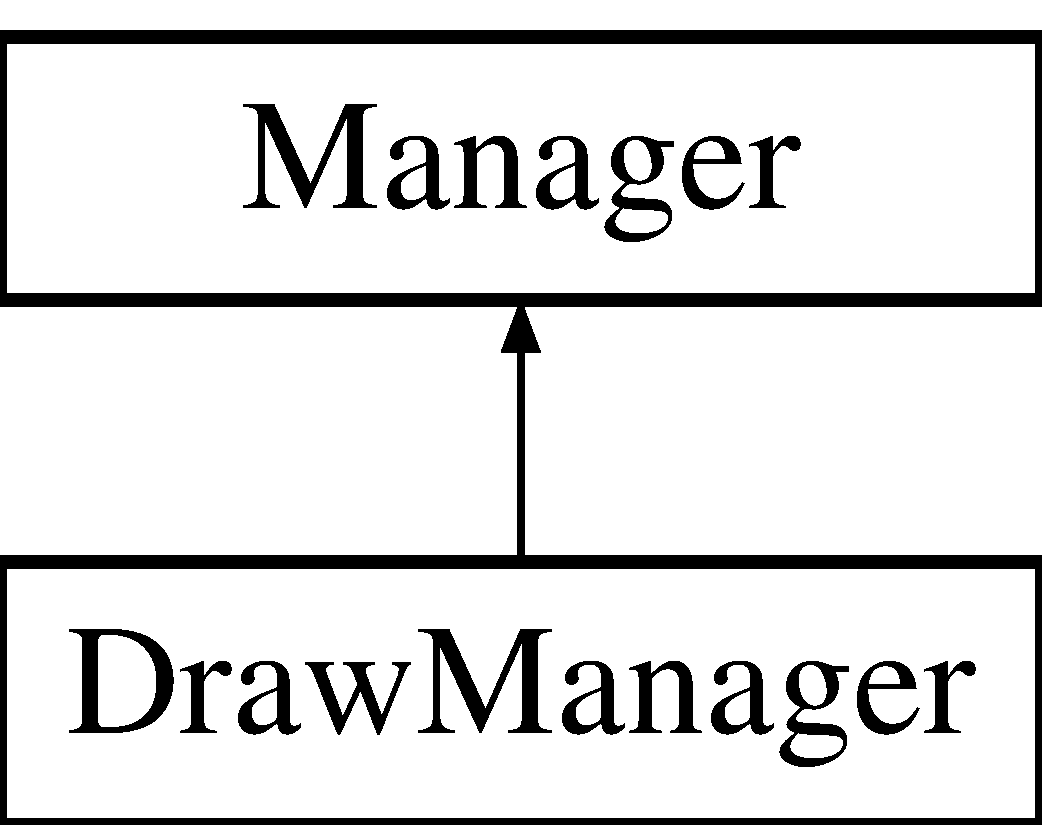
\includegraphics[height=2.000000cm]{classDrawManager}
\end{center}
\end{figure}
\subsection*{Public Member Functions}
\begin{DoxyCompactItemize}
\item 
\hyperlink{classDrawManager_a9a1e8b606471661af565479f7366bf21}{Draw\-Manager} ()
\begin{DoxyCompactList}\small\item\em Draw manager object constructor. \end{DoxyCompactList}\item 
virtual void \hyperlink{classDrawManager_a2c48a7d348b9f6961f2b615015dc482f}{manage} (\hyperlink{classGameStateData}{Game\-State\-Data} \&game\-\_\-state\-\_\-container, std\-::shared\-\_\-ptr$<$ \hyperlink{classDisplay}{Display} $>$ display)
\begin{DoxyCompactList}\small\item\em Drawing management cycle. \end{DoxyCompactList}\item 
void \hyperlink{classDrawManager_aea3804a9564e6185eec3750f5ff4e33f}{add\-New\-Entity} (const std\-::weak\-\_\-ptr$<$ \hyperlink{classDeletable}{Deletable} $>$ new\-\_\-entity)
\begin{DoxyCompactList}\small\item\em Adds a pointer to a drawable object. \end{DoxyCompactList}\item 
virtual \hyperlink{classDrawManager_ab2cbca4d18cb8838662754bb01585a9a}{$\sim$\-Draw\-Manager} ()
\end{DoxyCompactItemize}
\subsection*{Private Member Functions}
\begin{DoxyCompactItemize}
\item 
void \hyperlink{classDrawManager_a450157950bdd23c27bc5dcdafdaa3101}{get\-Tank\-Draw\-Info} (std\-::shared\-\_\-ptr$<$ \hyperlink{classDeletable}{Deletable} $>$ draw\-\_\-entity\-\_\-sp, \hyperlink{structsprite__draw__info}{sprite\-\_\-draw\-\_\-info} \&draw\-\_\-info)
\begin{DoxyCompactList}\small\item\em Gets info for tank to be drawn. \end{DoxyCompactList}\item 
void \hyperlink{classDrawManager_ae85d0a7a0c8b6c2a3abb0a617d8599ea}{get\-Missile\-Draw\-Info} (std\-::shared\-\_\-ptr$<$ \hyperlink{classDeletable}{Deletable} $>$ draw\-\_\-entity\-\_\-sp, \hyperlink{structsprite__draw__info}{sprite\-\_\-draw\-\_\-info} \&draw\-\_\-info)
\begin{DoxyCompactList}\small\item\em Gets info for missile to be drawn. \end{DoxyCompactList}\item 
void \hyperlink{classDrawManager_ac82e7f4f521c0a6eda4551c7182b782e}{get\-Mine\-Draw\-Info} (std\-::shared\-\_\-ptr$<$ \hyperlink{classDeletable}{Deletable} $>$ draw\-\_\-entity\-\_\-sp, \hyperlink{structsprite__draw__info}{sprite\-\_\-draw\-\_\-info} \&draw\-\_\-info)
\begin{DoxyCompactList}\small\item\em Gets info for mine to be drawn. \end{DoxyCompactList}\item 
void \hyperlink{classDrawManager_a41ad9837106a08143f5799c2e50535ff}{get\-Barrier\-Draw\-Info} (std\-::shared\-\_\-ptr$<$ \hyperlink{classDeletable}{Deletable} $>$ draw\-\_\-entity\-\_\-sp, \hyperlink{structsprite__draw__info}{sprite\-\_\-draw\-\_\-info} \&draw\-\_\-info)
\begin{DoxyCompactList}\small\item\em Gets info for barrier to be drawn. \end{DoxyCompactList}\item 
void \hyperlink{classDrawManager_ab63c01f42532b275a095c09e0a06cad9}{get\-Turret\-Draw\-Info} (std\-::shared\-\_\-ptr$<$ \hyperlink{classDeletable}{Deletable} $>$ draw\-\_\-entity\-\_\-sp, \hyperlink{structsprite__draw__info}{sprite\-\_\-draw\-\_\-info} \&draw\-\_\-info)
\begin{DoxyCompactList}\small\item\em Gets info for turret to be drawn. \end{DoxyCompactList}\item 
void \hyperlink{classDrawManager_a7ca495b3e5f25cbf2d56cc7e48ff3dce}{get\-Draw\-Position} (std\-::shared\-\_\-ptr$<$ \hyperlink{classDeletable}{Deletable} $>$ draw\-\_\-entity\-\_\-sp, \hyperlink{structsprite__draw__info}{sprite\-\_\-draw\-\_\-info} \&draw\-\_\-info)
\begin{DoxyCompactList}\small\item\em Gets info for an entity to be drawn. \end{DoxyCompactList}\end{DoxyCompactItemize}
\subsection*{Private Attributes}
\begin{DoxyCompactItemize}
\item 
std\-::vector$<$ std\-::weak\-\_\-ptr\\*
$<$ \hyperlink{classDeletable}{Deletable} $>$ $>$ \hyperlink{classDrawManager_a87982f3a0af2ece0a3a431a8f2fe4478}{\-\_\-drawables}
\begin{DoxyCompactList}\small\item\em Pointers to all drawable entites within the game world. \end{DoxyCompactList}\item 
\hyperlink{classSpriteDimensions}{Sprite\-Dimensions} \hyperlink{classDrawManager_a2cdf54bc1c47a4683f761af0c8ade8e9}{\-\_\-sprite\-\_\-dimensions}
\begin{DoxyCompactList}\small\item\em Private data object that holds sprite dimension info. \end{DoxyCompactList}\end{DoxyCompactItemize}


\subsection{Detailed Description}
\hyperlink{classManager}{Manager} class responsible for preparing draw data. 

Definition at line 24 of file Draw\-Manager.\-h.



\subsection{Constructor \& Destructor Documentation}
\hypertarget{classDrawManager_a9a1e8b606471661af565479f7366bf21}{\index{Draw\-Manager@{Draw\-Manager}!Draw\-Manager@{Draw\-Manager}}
\index{Draw\-Manager@{Draw\-Manager}!DrawManager@{Draw\-Manager}}
\subsubsection[{Draw\-Manager}]{\setlength{\rightskip}{0pt plus 5cm}Draw\-Manager\-::\-Draw\-Manager (
\begin{DoxyParamCaption}
{}
\end{DoxyParamCaption}
)}}\label{classDrawManager_a9a1e8b606471661af565479f7366bf21}


Draw manager object constructor. 

Create the sprite dimensions object 

Definition at line 18 of file Draw\-Manager.\-cpp.


\begin{DoxyCode}
18                         :
19     \hyperlink{classDrawManager_a2cdf54bc1c47a4683f761af0c8ade8e9}{\_sprite\_dimensions}()
20 \{
21 
22 \}
\end{DoxyCode}
\hypertarget{classDrawManager_ab2cbca4d18cb8838662754bb01585a9a}{\index{Draw\-Manager@{Draw\-Manager}!$\sim$\-Draw\-Manager@{$\sim$\-Draw\-Manager}}
\index{$\sim$\-Draw\-Manager@{$\sim$\-Draw\-Manager}!DrawManager@{Draw\-Manager}}
\subsubsection[{$\sim$\-Draw\-Manager}]{\setlength{\rightskip}{0pt plus 5cm}Draw\-Manager\-::$\sim$\-Draw\-Manager (
\begin{DoxyParamCaption}
{}
\end{DoxyParamCaption}
)\hspace{0.3cm}{\ttfamily [virtual]}}}\label{classDrawManager_ab2cbca4d18cb8838662754bb01585a9a}


Definition at line 209 of file Draw\-Manager.\-cpp.


\begin{DoxyCode}
210 \{
211 
212 \}
\end{DoxyCode}


\subsection{Member Function Documentation}
\hypertarget{classDrawManager_aea3804a9564e6185eec3750f5ff4e33f}{\index{Draw\-Manager@{Draw\-Manager}!add\-New\-Entity@{add\-New\-Entity}}
\index{add\-New\-Entity@{add\-New\-Entity}!DrawManager@{Draw\-Manager}}
\subsubsection[{add\-New\-Entity}]{\setlength{\rightskip}{0pt plus 5cm}void Draw\-Manager\-::add\-New\-Entity (
\begin{DoxyParamCaption}
\item[{const std\-::weak\-\_\-ptr$<$ {\bf Deletable} $>$}]{new\-\_\-entity}
\end{DoxyParamCaption}
)}}\label{classDrawManager_aea3804a9564e6185eec3750f5ff4e33f}


Adds a pointer to a drawable object. 

A weak pointer is saved to the private vector of the \hyperlink{classDrawManager}{Draw\-Manager} 
\begin{DoxyParams}{Parameters}
{\em new\-\_\-entity} & \-:\-: weak pointer to entity that will be added \\
\hline
\end{DoxyParams}


Definition at line 203 of file Draw\-Manager.\-cpp.



References \-\_\-drawables.



Referenced by Game\-::add\-Deletable(), and main().


\begin{DoxyCode}
204 \{
205     \hyperlink{classDrawManager_a87982f3a0af2ece0a3a431a8f2fe4478}{\_drawables}.push\_back(new\_entity);
206 \}
\end{DoxyCode}
\hypertarget{classDrawManager_a41ad9837106a08143f5799c2e50535ff}{\index{Draw\-Manager@{Draw\-Manager}!get\-Barrier\-Draw\-Info@{get\-Barrier\-Draw\-Info}}
\index{get\-Barrier\-Draw\-Info@{get\-Barrier\-Draw\-Info}!DrawManager@{Draw\-Manager}}
\subsubsection[{get\-Barrier\-Draw\-Info}]{\setlength{\rightskip}{0pt plus 5cm}void Draw\-Manager\-::get\-Barrier\-Draw\-Info (
\begin{DoxyParamCaption}
\item[{std\-::shared\-\_\-ptr$<$ {\bf Deletable} $>$}]{draw\-\_\-entity\-\_\-sp, }
\item[{{\bf sprite\-\_\-draw\-\_\-info} \&}]{draw\-\_\-info}
\end{DoxyParamCaption}
)\hspace{0.3cm}{\ttfamily [private]}}}\label{classDrawManager_a41ad9837106a08143f5799c2e50535ff}


Gets info for barrier to be drawn. 

This info includs the origin and position of the barrier. 
\begin{DoxyParams}{Parameters}
{\em draw\-\_\-entity\-\_\-sp} & \-:\-: shared pointer to the object from which info will be extracted \\
\hline
{\em draw\-\_\-info} & \-:\-: Info that will be updated with the entity draw position info. \\
\hline
\end{DoxyParams}


Definition at line 144 of file Draw\-Manager.\-cpp.



References \-\_\-sprite\-\_\-dimensions, Sprite\-Dimensions\-::barrier\-\_\-sprite\-\_\-x, Sprite\-Dimensions\-::barrier\-\_\-sprite\-\_\-y, get\-Draw\-Position(), sprite\-\_\-draw\-\_\-info\-::origin, coordinate\-::x, and coordinate\-::y.



Referenced by manage().


\begin{DoxyCode}
145 \{
146     draw\_info.\hyperlink{structsprite__draw__info_a7c12e335ba1fc83156a05a568d38a179}{origin}.\hyperlink{structcoordinate_acde0819ef9d30b7ce25b7d833d3df327}{x} = \hyperlink{classDrawManager_a2cdf54bc1c47a4683f761af0c8ade8e9}{\_sprite\_dimensions}.
      \hyperlink{classSpriteDimensions_abcc491d376f31d36013e4f2396dbc408}{barrier\_sprite\_x}/2;
147     draw\_info.\hyperlink{structsprite__draw__info_a7c12e335ba1fc83156a05a568d38a179}{origin}.\hyperlink{structcoordinate_ad48911206c84b1a8306a7023900ff622}{y} = \hyperlink{classDrawManager_a2cdf54bc1c47a4683f761af0c8ade8e9}{\_sprite\_dimensions}.
      \hyperlink{classSpriteDimensions_abad79766e2254e365d3455b3471a5d0a}{barrier\_sprite\_y}/2;
148     \hyperlink{classDrawManager_a7ca495b3e5f25cbf2d56cc7e48ff3dce}{getDrawPosition}(draw\_entity\_sp, draw\_info);
149 \}
\end{DoxyCode}
\hypertarget{classDrawManager_a7ca495b3e5f25cbf2d56cc7e48ff3dce}{\index{Draw\-Manager@{Draw\-Manager}!get\-Draw\-Position@{get\-Draw\-Position}}
\index{get\-Draw\-Position@{get\-Draw\-Position}!DrawManager@{Draw\-Manager}}
\subsubsection[{get\-Draw\-Position}]{\setlength{\rightskip}{0pt plus 5cm}void Draw\-Manager\-::get\-Draw\-Position (
\begin{DoxyParamCaption}
\item[{std\-::shared\-\_\-ptr$<$ {\bf Deletable} $>$}]{draw\-\_\-entity\-\_\-sp, }
\item[{{\bf sprite\-\_\-draw\-\_\-info} \&}]{draw\-\_\-info}
\end{DoxyParamCaption}
)\hspace{0.3cm}{\ttfamily [private]}}}\label{classDrawManager_a7ca495b3e5f25cbf2d56cc7e48ff3dce}


Gets info for an entity to be drawn. 

This info includs the origin and position of the entity. 
\begin{DoxyParams}{Parameters}
{\em draw\-\_\-entity\-\_\-sp} & \-:\-: shared pointer to the object from which info will be extracted \\
\hline
{\em draw\-\_\-info} & \-:\-: Info that will be updated with the entity draw position info. \\
\hline
\end{DoxyParams}


Definition at line 192 of file Draw\-Manager.\-cpp.



References sprite\-\_\-draw\-\_\-info\-::draw\-\_\-pos, sprite\-\_\-draw\-\_\-info\-::rotation, coordinate\-::x, and coordinate\-::y.



Referenced by get\-Barrier\-Draw\-Info(), get\-Mine\-Draw\-Info(), get\-Missile\-Draw\-Info(), get\-Tank\-Draw\-Info(), and get\-Turret\-Draw\-Info().


\begin{DoxyCode}
193 \{
194     draw\_info.\hyperlink{structsprite__draw__info_acf0a863cddf497e364e3cdc9c46b8564}{draw\_pos}.\hyperlink{structcoordinate_acde0819ef9d30b7ce25b7d833d3df327}{x} = draw\_entity\_sp->getDrawPositionX();
195     draw\_info.\hyperlink{structsprite__draw__info_acf0a863cddf497e364e3cdc9c46b8564}{draw\_pos}.\hyperlink{structcoordinate_ad48911206c84b1a8306a7023900ff622}{y} = draw\_entity\_sp->getDrawPositionY();
196     draw\_info.\hyperlink{structsprite__draw__info_a41292dd9fa6ca00d553a6c93f18e2a40}{rotation} = draw\_entity\_sp->getDrawRotation();
197 \}
\end{DoxyCode}
\hypertarget{classDrawManager_ac82e7f4f521c0a6eda4551c7182b782e}{\index{Draw\-Manager@{Draw\-Manager}!get\-Mine\-Draw\-Info@{get\-Mine\-Draw\-Info}}
\index{get\-Mine\-Draw\-Info@{get\-Mine\-Draw\-Info}!DrawManager@{Draw\-Manager}}
\subsubsection[{get\-Mine\-Draw\-Info}]{\setlength{\rightskip}{0pt plus 5cm}void Draw\-Manager\-::get\-Mine\-Draw\-Info (
\begin{DoxyParamCaption}
\item[{std\-::shared\-\_\-ptr$<$ {\bf Deletable} $>$}]{draw\-\_\-entity\-\_\-sp, }
\item[{{\bf sprite\-\_\-draw\-\_\-info} \&}]{draw\-\_\-info}
\end{DoxyParamCaption}
)\hspace{0.3cm}{\ttfamily [private]}}}\label{classDrawManager_ac82e7f4f521c0a6eda4551c7182b782e}


Gets info for mine to be drawn. 

This info includs the origin and position of the mine. 
\begin{DoxyParams}{Parameters}
{\em draw\-\_\-entity\-\_\-sp} & \-:\-: shared pointer to the object from which info will be extracted \\
\hline
{\em draw\-\_\-info} & \-:\-: Info that will be updated with the entity draw position info. \\
\hline
\end{DoxyParams}


Definition at line 168 of file Draw\-Manager.\-cpp.



References \-\_\-sprite\-\_\-dimensions, get\-Draw\-Position(), Sprite\-Dimensions\-::mine\-\_\-sprite\-\_\-x, Sprite\-Dimensions\-::mine\-\_\-sprite\-\_\-y, sprite\-\_\-draw\-\_\-info\-::origin, coordinate\-::x, and coordinate\-::y.



Referenced by manage().


\begin{DoxyCode}
169 \{
170     draw\_info.\hyperlink{structsprite__draw__info_a7c12e335ba1fc83156a05a568d38a179}{origin}.\hyperlink{structcoordinate_acde0819ef9d30b7ce25b7d833d3df327}{x} = \hyperlink{classDrawManager_a2cdf54bc1c47a4683f761af0c8ade8e9}{\_sprite\_dimensions}.
      \hyperlink{classSpriteDimensions_af7f442b00b4a2d9d8b9ad47371a0018f}{mine\_sprite\_x}/2;
171     draw\_info.\hyperlink{structsprite__draw__info_a7c12e335ba1fc83156a05a568d38a179}{origin}.\hyperlink{structcoordinate_ad48911206c84b1a8306a7023900ff622}{y} = \hyperlink{classDrawManager_a2cdf54bc1c47a4683f761af0c8ade8e9}{\_sprite\_dimensions}.
      \hyperlink{classSpriteDimensions_a256b5245430fc54ae2cace272260dbe1}{mine\_sprite\_y}/2;
172     \hyperlink{classDrawManager_a7ca495b3e5f25cbf2d56cc7e48ff3dce}{getDrawPosition}(draw\_entity\_sp, draw\_info);
173 \}
\end{DoxyCode}
\hypertarget{classDrawManager_ae85d0a7a0c8b6c2a3abb0a617d8599ea}{\index{Draw\-Manager@{Draw\-Manager}!get\-Missile\-Draw\-Info@{get\-Missile\-Draw\-Info}}
\index{get\-Missile\-Draw\-Info@{get\-Missile\-Draw\-Info}!DrawManager@{Draw\-Manager}}
\subsubsection[{get\-Missile\-Draw\-Info}]{\setlength{\rightskip}{0pt plus 5cm}void Draw\-Manager\-::get\-Missile\-Draw\-Info (
\begin{DoxyParamCaption}
\item[{std\-::shared\-\_\-ptr$<$ {\bf Deletable} $>$}]{draw\-\_\-entity\-\_\-sp, }
\item[{{\bf sprite\-\_\-draw\-\_\-info} \&}]{draw\-\_\-info}
\end{DoxyParamCaption}
)\hspace{0.3cm}{\ttfamily [private]}}}\label{classDrawManager_ae85d0a7a0c8b6c2a3abb0a617d8599ea}


Gets info for missile to be drawn. 

This info includs the origin and position of the missile. 
\begin{DoxyParams}{Parameters}
{\em draw\-\_\-entity\-\_\-sp} & \-:\-: shared pointer to the object from which info will be extracted \\
\hline
{\em draw\-\_\-info} & \-:\-: Info that will be updated with the entity draw position info. \\
\hline
\end{DoxyParams}


Definition at line 156 of file Draw\-Manager.\-cpp.



References \-\_\-sprite\-\_\-dimensions, get\-Draw\-Position(), Sprite\-Dimensions\-::missile\-\_\-sprite\-\_\-x, Sprite\-Dimensions\-::missile\-\_\-sprite\-\_\-y, sprite\-\_\-draw\-\_\-info\-::origin, coordinate\-::x, and coordinate\-::y.



Referenced by manage().


\begin{DoxyCode}
157 \{
158     draw\_info.\hyperlink{structsprite__draw__info_a7c12e335ba1fc83156a05a568d38a179}{origin}.\hyperlink{structcoordinate_acde0819ef9d30b7ce25b7d833d3df327}{x} = \hyperlink{classDrawManager_a2cdf54bc1c47a4683f761af0c8ade8e9}{\_sprite\_dimensions}.
      \hyperlink{classSpriteDimensions_a0c406c32caf5ea7841c763100dd83ecf}{missile\_sprite\_x}/2;
159     draw\_info.\hyperlink{structsprite__draw__info_a7c12e335ba1fc83156a05a568d38a179}{origin}.\hyperlink{structcoordinate_ad48911206c84b1a8306a7023900ff622}{y} = \hyperlink{classDrawManager_a2cdf54bc1c47a4683f761af0c8ade8e9}{\_sprite\_dimensions}.
      \hyperlink{classSpriteDimensions_adcf501d11ae383d24cbbe5b526585f86}{missile\_sprite\_y}/2;
160     \hyperlink{classDrawManager_a7ca495b3e5f25cbf2d56cc7e48ff3dce}{getDrawPosition}(draw\_entity\_sp, draw\_info);
161 \}
\end{DoxyCode}
\hypertarget{classDrawManager_a450157950bdd23c27bc5dcdafdaa3101}{\index{Draw\-Manager@{Draw\-Manager}!get\-Tank\-Draw\-Info@{get\-Tank\-Draw\-Info}}
\index{get\-Tank\-Draw\-Info@{get\-Tank\-Draw\-Info}!DrawManager@{Draw\-Manager}}
\subsubsection[{get\-Tank\-Draw\-Info}]{\setlength{\rightskip}{0pt plus 5cm}void Draw\-Manager\-::get\-Tank\-Draw\-Info (
\begin{DoxyParamCaption}
\item[{std\-::shared\-\_\-ptr$<$ {\bf Deletable} $>$}]{draw\-\_\-entity\-\_\-sp, }
\item[{{\bf sprite\-\_\-draw\-\_\-info} \&}]{draw\-\_\-info}
\end{DoxyParamCaption}
)\hspace{0.3cm}{\ttfamily [private]}}}\label{classDrawManager_a450157950bdd23c27bc5dcdafdaa3101}


Gets info for tank to be drawn. 

This info includs the origin and position of the tank. 
\begin{DoxyParams}{Parameters}
{\em draw\-\_\-entity\-\_\-sp} & \-:\-: shared pointer to the object from which info will be extracted \\
\hline
{\em draw\-\_\-info} & \-:\-: Info that will be updated with the entity draw position info. \\
\hline
\end{DoxyParams}


Definition at line 132 of file Draw\-Manager.\-cpp.



References \-\_\-sprite\-\_\-dimensions, get\-Draw\-Position(), sprite\-\_\-draw\-\_\-info\-::origin, Sprite\-Dimensions\-::tank\-\_\-sprite\-\_\-x, Sprite\-Dimensions\-::tank\-\_\-sprite\-\_\-y, coordinate\-::x, and coordinate\-::y.



Referenced by manage().


\begin{DoxyCode}
133 \{
134     draw\_info.\hyperlink{structsprite__draw__info_a7c12e335ba1fc83156a05a568d38a179}{origin}.\hyperlink{structcoordinate_acde0819ef9d30b7ce25b7d833d3df327}{x} = \hyperlink{classDrawManager_a2cdf54bc1c47a4683f761af0c8ade8e9}{\_sprite\_dimensions}.
      \hyperlink{classSpriteDimensions_a9d7ddd6f707798f86ced573e28f9eea0}{tank\_sprite\_x}/2;
135     draw\_info.\hyperlink{structsprite__draw__info_a7c12e335ba1fc83156a05a568d38a179}{origin}.\hyperlink{structcoordinate_ad48911206c84b1a8306a7023900ff622}{y} = \hyperlink{classDrawManager_a2cdf54bc1c47a4683f761af0c8ade8e9}{\_sprite\_dimensions}.
      \hyperlink{classSpriteDimensions_abe1930e59ce44b9bdc0e6b363b668f7d}{tank\_sprite\_y}/2;
136     \hyperlink{classDrawManager_a7ca495b3e5f25cbf2d56cc7e48ff3dce}{getDrawPosition}(draw\_entity\_sp, draw\_info);
137 \}
\end{DoxyCode}
\hypertarget{classDrawManager_ab63c01f42532b275a095c09e0a06cad9}{\index{Draw\-Manager@{Draw\-Manager}!get\-Turret\-Draw\-Info@{get\-Turret\-Draw\-Info}}
\index{get\-Turret\-Draw\-Info@{get\-Turret\-Draw\-Info}!DrawManager@{Draw\-Manager}}
\subsubsection[{get\-Turret\-Draw\-Info}]{\setlength{\rightskip}{0pt plus 5cm}void Draw\-Manager\-::get\-Turret\-Draw\-Info (
\begin{DoxyParamCaption}
\item[{std\-::shared\-\_\-ptr$<$ {\bf Deletable} $>$}]{draw\-\_\-entity\-\_\-sp, }
\item[{{\bf sprite\-\_\-draw\-\_\-info} \&}]{draw\-\_\-info}
\end{DoxyParamCaption}
)\hspace{0.3cm}{\ttfamily [private]}}}\label{classDrawManager_ab63c01f42532b275a095c09e0a06cad9}


Gets info for turret to be drawn. 

This info includs the origin and position of the turret. 
\begin{DoxyParams}{Parameters}
{\em draw\-\_\-entity\-\_\-sp} & \-:\-: shared pointer to the object from which info will be extracted \\
\hline
{\em draw\-\_\-info} & \-:\-: Info that will be updated with the entity draw position info. \\
\hline
\end{DoxyParams}


Definition at line 180 of file Draw\-Manager.\-cpp.



References \-\_\-sprite\-\_\-dimensions, get\-Draw\-Position(), sprite\-\_\-draw\-\_\-info\-::origin, Sprite\-Dimensions\-::turret\-\_\-sprite\-\_\-x, Sprite\-Dimensions\-::turret\-\_\-sprite\-\_\-y, coordinate\-::x, and coordinate\-::y.



Referenced by manage().


\begin{DoxyCode}
181 \{
182     draw\_info.\hyperlink{structsprite__draw__info_a7c12e335ba1fc83156a05a568d38a179}{origin}.\hyperlink{structcoordinate_acde0819ef9d30b7ce25b7d833d3df327}{x} = \hyperlink{classDrawManager_a2cdf54bc1c47a4683f761af0c8ade8e9}{\_sprite\_dimensions}.
      \hyperlink{classSpriteDimensions_ad876e1e5dea420fe80462709c8ec2d5c}{turret\_sprite\_x}/2;
183     draw\_info.\hyperlink{structsprite__draw__info_a7c12e335ba1fc83156a05a568d38a179}{origin}.\hyperlink{structcoordinate_ad48911206c84b1a8306a7023900ff622}{y} = \hyperlink{classDrawManager_a2cdf54bc1c47a4683f761af0c8ade8e9}{\_sprite\_dimensions}.
      \hyperlink{classSpriteDimensions_a1b808c73bd915776ec6b8c10120adeae}{turret\_sprite\_y}/2;
184     \hyperlink{classDrawManager_a7ca495b3e5f25cbf2d56cc7e48ff3dce}{getDrawPosition}(draw\_entity\_sp, draw\_info);
185 \}
\end{DoxyCode}
\hypertarget{classDrawManager_a2c48a7d348b9f6961f2b615015dc482f}{\index{Draw\-Manager@{Draw\-Manager}!manage@{manage}}
\index{manage@{manage}!DrawManager@{Draw\-Manager}}
\subsubsection[{manage}]{\setlength{\rightskip}{0pt plus 5cm}void Draw\-Manager\-::manage (
\begin{DoxyParamCaption}
\item[{{\bf Game\-State\-Data} \&}]{game\-\_\-state\-\_\-container, }
\item[{std\-::shared\-\_\-ptr$<$ {\bf Display} $>$}]{display}
\end{DoxyParamCaption}
)\hspace{0.3cm}{\ttfamily [virtual]}}}\label{classDrawManager_a2c48a7d348b9f6961f2b615015dc482f}


Drawing management cycle. 

Main function of the \hyperlink{classDrawManager}{Draw\-Manager}. The display object is accessable within here. The \hyperlink{classDrawManager}{Draw\-Manager} first gets the display to clear the window and display the background. Then all drawables are iterated through and drawn. Info is collected based on the entity that will be drawn. This information is passed to the display object which actually performs the drawing. 
\begin{DoxyParams}{Parameters}
{\em game\-\_\-state\-\_\-container} & \-:\-: \hyperlink{classGame}{Game} data that hold the time and player scores to be drawn \\
\hline
{\em display} & \-:\-: The display to which display information is passed. \\
\hline
\end{DoxyParams}


Definition at line 32 of file Draw\-Manager.\-cpp.



References \-\_\-drawables, barrier, draw\-\_\-strings\-::game\-\_\-time, get\-Barrier\-Draw\-Info(), Game\-State\-Data\-::get\-Game\-Time(), get\-Mine\-Draw\-Info(), get\-Missile\-Draw\-Info(), Game\-State\-Data\-::get\-P1\-Score(), Game\-State\-Data\-::get\-P2\-Score(), get\-Tank\-Draw\-Info(), get\-Turret\-Draw\-Info(), p1\-\_\-mine, p1\-\_\-missile, draw\-\_\-strings\-::p1\-\_\-score, p1\-\_\-tank, p2\-\_\-mine, p2\-\_\-missile, draw\-\_\-strings\-::p2\-\_\-score, p2\-\_\-tank, turret, and turret\-\_\-missile.



Referenced by main(), and Game\-::run\-All\-Managers().


\begin{DoxyCode}
33 \{
34     display->clear();
35     display->drawBackground();
36 
37     \hyperlink{structsprite__draw__info}{sprite\_draw\_info} draw\_info;
38     \textcolor{comment}{//Used to traverse the vector of drawables held by DrawManager}
39     \textcolor{keyword}{auto} draw\_itterator = \hyperlink{classDrawManager_a87982f3a0af2ece0a3a431a8f2fe4478}{\_drawables}.begin();
40 
41     \textcolor{comment}{//Loop through Array of Drawables and draw the corresponding sprite}
42     \textcolor{keywordflow}{for}(;draw\_itterator != \hyperlink{classDrawManager_a87982f3a0af2ece0a3a431a8f2fe4478}{\_drawables}.end();)
43     \{
44         \textcolor{comment}{//Deref itterator to weak pointer}
45         std::weak\_ptr<Deletable> draw\_entity\_wp = (*draw\_itterator);
46         \textcolor{comment}{//Convert to shared pointer}
47         std::shared\_ptr<Deletable> draw\_entity\_sp = draw\_entity\_wp.lock();
48         \textcolor{comment}{//Check to see if the entity still exists}
49         \textcolor{keywordflow}{if}(draw\_entity\_sp)
50         \{
51             \textcolor{keywordflow}{switch} (draw\_entity\_sp->getType())
52             \{
53                 \textcolor{keywordflow}{case} \hyperlink{Structures_8h_a6d8f83e710b27d4f86c45f0bb77066e3a31fa78b2b7dd774f5158a16ef230932e}{p1\_tank}:
54                     \hyperlink{classDrawManager_a450157950bdd23c27bc5dcdafdaa3101}{getTankDrawInfo}(draw\_entity\_sp, draw\_info);
55                     display->drawEntity(\hyperlink{Structures_8h_a6d8f83e710b27d4f86c45f0bb77066e3a31fa78b2b7dd774f5158a16ef230932e}{p1\_tank}, draw\_info);
56                     \textcolor{keywordflow}{break};
57 
58                 \textcolor{keywordflow}{case} \hyperlink{Structures_8h_a6d8f83e710b27d4f86c45f0bb77066e3a3d48d62c7b88e7ee171698fe56dc9e59}{p2\_tank}:
59                     \hyperlink{classDrawManager_a450157950bdd23c27bc5dcdafdaa3101}{getTankDrawInfo}(draw\_entity\_sp, draw\_info);
60                     display->drawEntity(\hyperlink{Structures_8h_a6d8f83e710b27d4f86c45f0bb77066e3a3d48d62c7b88e7ee171698fe56dc9e59}{p2\_tank}, draw\_info);
61                     \textcolor{keywordflow}{break};
62 
63                 \textcolor{keywordflow}{case} \hyperlink{Structures_8h_a6d8f83e710b27d4f86c45f0bb77066e3a6fb040c958f554e1d8320926b700b59d}{barrier}:
64                     \hyperlink{classDrawManager_a41ad9837106a08143f5799c2e50535ff}{getBarrierDrawInfo}(draw\_entity\_sp, draw\_info);
65                     display->drawEntity(\hyperlink{Structures_8h_a6d8f83e710b27d4f86c45f0bb77066e3a6fb040c958f554e1d8320926b700b59d}{barrier}, draw\_info);
66                     \textcolor{keywordflow}{break};
67 
68                 \textcolor{keywordflow}{case} \hyperlink{Structures_8h_a6d8f83e710b27d4f86c45f0bb77066e3af89bc631e9b0140ed004b5ce2db5330c}{p1\_missile}:
69                     \hyperlink{classDrawManager_ae85d0a7a0c8b6c2a3abb0a617d8599ea}{getMissileDrawInfo}(draw\_entity\_sp, draw\_info);
70                     display->drawEntity(\hyperlink{Structures_8h_a6d8f83e710b27d4f86c45f0bb77066e3af89bc631e9b0140ed004b5ce2db5330c}{p1\_missile}, draw\_info);
71                     \textcolor{keywordflow}{break};
72 
73                 \textcolor{keywordflow}{case} \hyperlink{Structures_8h_a6d8f83e710b27d4f86c45f0bb77066e3a47100170e5852d632dfe65582a18256d}{p2\_missile}:
74                     \hyperlink{classDrawManager_ae85d0a7a0c8b6c2a3abb0a617d8599ea}{getMissileDrawInfo}(draw\_entity\_sp, draw\_info);
75                     display->drawEntity(\hyperlink{Structures_8h_a6d8f83e710b27d4f86c45f0bb77066e3a47100170e5852d632dfe65582a18256d}{p2\_missile}, draw\_info);
76                     \textcolor{keywordflow}{break};
77 
78                 \textcolor{keywordflow}{case} \hyperlink{Structures_8h_a6d8f83e710b27d4f86c45f0bb77066e3afc52e626787e982ae5d0a747bed6666d}{p1\_mine}:
79                     \hyperlink{classDrawManager_ac82e7f4f521c0a6eda4551c7182b782e}{getMineDrawInfo}(draw\_entity\_sp, draw\_info);
80                     display->drawEntity(\hyperlink{Structures_8h_a6d8f83e710b27d4f86c45f0bb77066e3afc52e626787e982ae5d0a747bed6666d}{p1\_mine}, draw\_info);
81                     \textcolor{keywordflow}{break};
82 
83                 \textcolor{keywordflow}{case} \hyperlink{Structures_8h_a6d8f83e710b27d4f86c45f0bb77066e3ada293b37940e64ec2cf6dbd2ae493d2b}{p2\_mine}:
84                     \hyperlink{classDrawManager_ac82e7f4f521c0a6eda4551c7182b782e}{getMineDrawInfo}(draw\_entity\_sp, draw\_info);
85                     display->drawEntity(\hyperlink{Structures_8h_a6d8f83e710b27d4f86c45f0bb77066e3ada293b37940e64ec2cf6dbd2ae493d2b}{p2\_mine}, draw\_info);
86                     \textcolor{keywordflow}{break};
87 
88                 \textcolor{keywordflow}{case} \hyperlink{Structures_8h_a6d8f83e710b27d4f86c45f0bb77066e3a85c730ac9ffc13ac94e6e860579928a1}{turret}:
89                     \hyperlink{classDrawManager_ab63c01f42532b275a095c09e0a06cad9}{getTurretDrawInfo}(draw\_entity\_sp, draw\_info);
90                     display->drawEntity(\hyperlink{Structures_8h_a6d8f83e710b27d4f86c45f0bb77066e3a85c730ac9ffc13ac94e6e860579928a1}{turret}, draw\_info);
91                     \textcolor{keywordflow}{break};
92 
93                 \textcolor{keywordflow}{case} \hyperlink{Structures_8h_a6d8f83e710b27d4f86c45f0bb77066e3a8f552a1e495ced5aa8775faa1b6a757b}{turret\_missile}:
94                     \hyperlink{classDrawManager_ae85d0a7a0c8b6c2a3abb0a617d8599ea}{getMissileDrawInfo}(draw\_entity\_sp, draw\_info);
95                     display->drawEntity(\hyperlink{Structures_8h_a6d8f83e710b27d4f86c45f0bb77066e3a8f552a1e495ced5aa8775faa1b6a757b}{turret\_missile}, draw\_info);
96                     \textcolor{keywordflow}{break};
97 
98                 \textcolor{keywordflow}{default}:
99                 \textcolor{keywordflow}{break};
100 
101             \} \textcolor{comment}{//Switch}
102             draw\_itterator++;
103         \} \textcolor{comment}{//if (pointer still valid)}
104         \textcolor{keywordflow}{else}
105             \hyperlink{classDrawManager_a87982f3a0af2ece0a3a431a8f2fe4478}{\_drawables}.erase(draw\_itterator);
106 
107     \} \textcolor{comment}{//for}
108 
109     \hyperlink{structdraw__strings}{draw\_strings} strings;
110 
111     std::ostringstream strs1; \textcolor{comment}{// convert to strings}
112     strs1 << game\_state\_container.\hyperlink{classGameStateData_a0cb5cf167da9dd1929c719778c5d3506}{getGameTime}();
113     strings.\hyperlink{structdraw__strings_a4d19f66b000d19861c475694328d9fce}{game\_time} = strs1.str();
114 
115     std::ostringstream strs2;
116     strs2 << game\_state\_container.\hyperlink{classGameStateData_ac4dbf8f19eb4abae6c6e674e1f0ad473}{getP1Score}();
117     strings.\hyperlink{structdraw__strings_a0d59a0f9e78f1c539dbe7959dcd9c3bb}{p1\_score} = strs2.str();
118 
119     std::ostringstream strs3;
120     strs3 << game\_state\_container.\hyperlink{classGameStateData_a024affaa547433a0feca091d2bc516b6}{getP2Score}();
121     strings.\hyperlink{structdraw__strings_a749fa74ab7403f436f100c546b073be8}{p2\_score} = strs3.str();
122 
123     display->drawText(strings);
124     display->display();
125 \}
\end{DoxyCode}


\subsection{Member Data Documentation}
\hypertarget{classDrawManager_a87982f3a0af2ece0a3a431a8f2fe4478}{\index{Draw\-Manager@{Draw\-Manager}!\-\_\-drawables@{\-\_\-drawables}}
\index{\-\_\-drawables@{\-\_\-drawables}!DrawManager@{Draw\-Manager}}
\subsubsection[{\-\_\-drawables}]{\setlength{\rightskip}{0pt plus 5cm}std\-::vector$<$std\-::weak\-\_\-ptr$<${\bf Deletable}$>$ $>$ Draw\-Manager\-::\-\_\-drawables\hspace{0.3cm}{\ttfamily [private]}}}\label{classDrawManager_a87982f3a0af2ece0a3a431a8f2fe4478}


Pointers to all drawable entites within the game world. 



Definition at line 34 of file Draw\-Manager.\-h.



Referenced by add\-New\-Entity(), and manage().

\hypertarget{classDrawManager_a2cdf54bc1c47a4683f761af0c8ade8e9}{\index{Draw\-Manager@{Draw\-Manager}!\-\_\-sprite\-\_\-dimensions@{\-\_\-sprite\-\_\-dimensions}}
\index{\-\_\-sprite\-\_\-dimensions@{\-\_\-sprite\-\_\-dimensions}!DrawManager@{Draw\-Manager}}
\subsubsection[{\-\_\-sprite\-\_\-dimensions}]{\setlength{\rightskip}{0pt plus 5cm}{\bf Sprite\-Dimensions} Draw\-Manager\-::\-\_\-sprite\-\_\-dimensions\hspace{0.3cm}{\ttfamily [private]}}}\label{classDrawManager_a2cdf54bc1c47a4683f761af0c8ade8e9}


Private data object that holds sprite dimension info. 



Definition at line 36 of file Draw\-Manager.\-h.



Referenced by get\-Barrier\-Draw\-Info(), get\-Mine\-Draw\-Info(), get\-Missile\-Draw\-Info(), get\-Tank\-Draw\-Info(), and get\-Turret\-Draw\-Info().



The documentation for this class was generated from the following files\-:\begin{DoxyCompactItemize}
\item 
\hyperlink{DrawManager_8h}{Draw\-Manager.\-h}\item 
\hyperlink{DrawManager_8cpp}{Draw\-Manager.\-cpp}\end{DoxyCompactItemize}

\hypertarget{classGame}{\section{Game Class Reference}
\label{classGame}\index{Game@{Game}}
}


Main class which runs the program loop.  




{\ttfamily \#include $<$Game.\-h$>$}

\subsection*{Public Member Functions}
\begin{DoxyCompactItemize}
\item 
\hyperlink{classGame_ad59df6562a58a614fda24622d3715b65}{Game} ()
\begin{DoxyCompactList}\small\item\em \hyperlink{classGame}{Game} object constructor. \end{DoxyCompactList}\item 
void \hyperlink{classGame_a6073fbea287e3bd28ae5eaf350559448}{run\-World} (std\-::shared\-\_\-ptr$<$ \hyperlink{classDisplay}{Display} $>$ display)
\begin{DoxyCompactList}\small\item\em Main program loop. \end{DoxyCompactList}\item 
\hyperlink{classGame_ae3d112ca6e0e55150d2fdbc704474530}{$\sim$\-Game} ()
\end{DoxyCompactItemize}
\subsection*{Private Member Functions}
\begin{DoxyCompactItemize}
\item 
void \hyperlink{classGame_ad0f1180499fb33b89deb50da6c1fdd78}{setup\-Initial\-Map} ()
\begin{DoxyCompactList}\small\item\em Sets up the game wolrd map. \end{DoxyCompactList}\item 
void \hyperlink{classGame_ad43265203e4e3e90ee91eb1fedbc06d4}{get\-Map\-Data} (std\-::vector$<$ std\-::vector$<$ char $>$$>$ \&map\-\_\-vector, std\-::ifstream \&map\-\_\-grid\-\_\-file)
\begin{DoxyCompactList}\small\item\em Reads map data from text file. \end{DoxyCompactList}\item 
void \hyperlink{classGame_a742dfb46a327c277b5b5711052919d21}{read\-Map\-Data} (const std\-::vector$<$ std\-::vector$<$ char $>$$>$ \&map\-\_\-vector)
\begin{DoxyCompactList}\small\item\em Reads the map data from the vector. \end{DoxyCompactList}\item 
void \hyperlink{classGame_a9fbdc107c782dba1f2debf7ee347bb7d}{check\-Keyboard\-Input} (\hyperlink{classActionData}{Action\-Data} \&action\-\_\-data\-\_\-container)
\begin{DoxyCompactList}\small\item\em Checks through all pressed control keys. \end{DoxyCompactList}\item 
void \hyperlink{classGame_a39814b41ab7d5bc1af48bed69500a2be}{run\-All\-Managers} (\hyperlink{classGameManagementData}{Game\-Management\-Data} \&game\-\_\-data\-\_\-container, std\-::shared\-\_\-ptr$<$ \hyperlink{classDisplay}{Display} $>$ display)
\begin{DoxyCompactList}\small\item\em All managers manage. \end{DoxyCompactList}\item 
void \hyperlink{classGame_abd126d710f269c525c2f26e290444cf7}{add\-New\-World\-Entity} (\hyperlink{classGameManagementData}{Game\-Management\-Data} \&game\-\_\-data\-\_\-container)
\begin{DoxyCompactList}\small\item\em Any new game entity is added here. \end{DoxyCompactList}\item 
void \hyperlink{classGame_ab77bec9aa745c5fb55794d0bbed4b235}{add\-New\-Tank} (\hyperlink{Structures_8h_a6d8f83e710b27d4f86c45f0bb77066e3}{entity\-\_\-type} player\-\_\-tank, float tank\-\_\-position\-X, float tank\-\_\-position\-Y, float rotation)
\begin{DoxyCompactList}\small\item\em Adds a new tank object. \end{DoxyCompactList}\item 
void \hyperlink{classGame_a2099d667dbb4574c4c9bed31eab2abb2}{add\-New\-Missile} (std\-::shared\-\_\-ptr$<$ \hyperlink{classDeletable}{Deletable} $>$ missile\-\_\-del\-\_\-sp)
\begin{DoxyCompactList}\small\item\em Adds a new missile object. \end{DoxyCompactList}\item 
void \hyperlink{classGame_afb856cf115b4c22af456a5424a37c915}{add\-New\-Mine} (std\-::shared\-\_\-ptr$<$ \hyperlink{classDeletable}{Deletable} $>$ mine\-\_\-del\-\_\-sp)
\begin{DoxyCompactList}\small\item\em Adds a new mine object. \end{DoxyCompactList}\item 
void \hyperlink{classGame_ada424b3c51aa8eca26cc9b51c2fe3604}{add\-New\-Turret} (float turret\-\_\-position\-X, float turret\-\_\-postion\-Y, float rotation)
\begin{DoxyCompactList}\small\item\em Adds a new turret object. \end{DoxyCompactList}\item 
void \hyperlink{classGame_a50b0e861ea3d882bf20017c9c759244d}{manage\-Respawns} (\hyperlink{classGameManagementData}{Game\-Management\-Data} \&game\-\_\-data\-\_\-container)
\begin{DoxyCompactList}\small\item\em Manages when a respawn needs to take place. \end{DoxyCompactList}\item 
void \hyperlink{classGame_a14fce36a80fcf6b59d6eba6af3ee23d2}{create\-Barrier} (int x, int y)
\begin{DoxyCompactList}\small\item\em Adds a new barrier object. \end{DoxyCompactList}\item 
void \hyperlink{classGame_abf5f8299e3e0889960a963546976817f}{add\-Deletable} (std\-::shared\-\_\-ptr$<$ \hyperlink{classDeletable}{Deletable} $>$ deletable\-\_\-sp)
\begin{DoxyCompactList}\small\item\em Adds entity to deletables vector. \end{DoxyCompactList}\item 
void \hyperlink{classGame_afece3314d2bda96eddb765a2da9ebdd0}{add\-Collidable} (std\-::shared\-\_\-ptr$<$ \hyperlink{classDeletable}{Deletable} $>$ collidable\-\_\-sp)
\begin{DoxyCompactList}\small\item\em Adds entity to collidables. \end{DoxyCompactList}\item 
void \hyperlink{classGame_a42545efdf0cdf4572d97fafba1c20dcd}{add\-Movable} (std\-::shared\-\_\-ptr$<$ \hyperlink{classDeletable}{Deletable} $>$ movable\-\_\-sp)
\begin{DoxyCompactList}\small\item\em Adds entity to movables. \end{DoxyCompactList}\item 
void \hyperlink{classGame_afb1552b97539822cb5aef6fcd08fa7b3}{add\-Trackable} (std\-::shared\-\_\-ptr$<$ \hyperlink{classDeletable}{Deletable} $>$ trackable\-\_\-sp)
\begin{DoxyCompactList}\small\item\em Adds entity to trackables. \end{DoxyCompactList}\item 
void \hyperlink{classGame_a97806aa1b86c7c908763a79b2d739439}{add\-Turretable} (std\-::shared\-\_\-ptr$<$ \hyperlink{classDeletable}{Deletable} $>$ trackable\-\_\-sp)
\begin{DoxyCompactList}\small\item\em Adds entity to turrets. \end{DoxyCompactList}\end{DoxyCompactItemize}
\subsection*{Private Attributes}
\begin{DoxyCompactItemize}
\item 
float \hyperlink{classGame_ac3d9582803715a82b0aa03ddc9d9b7f6}{\-\_\-player1\-\_\-start\-X}
\begin{DoxyCompactList}\small\item\em Player 1 starting x position. \end{DoxyCompactList}\item 
float \hyperlink{classGame_ac86e7845910feac197a8396c9eedcae9}{\-\_\-player1\-\_\-start\-Y}
\begin{DoxyCompactList}\small\item\em Player 1 starting y position. \end{DoxyCompactList}\item 
float \hyperlink{classGame_ac3fb65efc81597149ea1c6951110f1b8}{\-\_\-player2\-\_\-start\-X}
\begin{DoxyCompactList}\small\item\em Player 2 starting x position. \end{DoxyCompactList}\item 
float \hyperlink{classGame_a62232949f4969880bad54622e180d9aa}{\-\_\-player2\-\_\-start\-Y}
\begin{DoxyCompactList}\small\item\em Player 2 starting y position. \end{DoxyCompactList}\item 
float \hyperlink{classGame_ad7a148e2de0c944863d8aaa78a075f74}{\-\_\-turret\-\_\-start\-X}
\begin{DoxyCompactList}\small\item\em \hyperlink{classTurret}{Turret} starting x position. \end{DoxyCompactList}\item 
float \hyperlink{classGame_ab875384f85be491849e480d7f91cfe93}{\-\_\-turret\-\_\-start\-Y}
\begin{DoxyCompactList}\small\item\em \hyperlink{classTurret}{Turret} starting y position. \end{DoxyCompactList}\item 
\hyperlink{classMoveManager}{Move\-Manager} \hyperlink{classGame_a2998c8ca6b641f19bca912c1aba2d54f}{\-\_\-move\-\_\-manager}
\begin{DoxyCompactList}\small\item\em Private object of the \hyperlink{classMoveManager}{Move\-Manager}. \end{DoxyCompactList}\item 
\hyperlink{classCollisionManager}{Collision\-Manager} \hyperlink{classGame_a434f5c076c3abc86944fb02e86edc432}{\-\_\-collision\-\_\-manager}
\begin{DoxyCompactList}\small\item\em Private object of the \hyperlink{classCollisionManager}{Collision\-Manager}. \end{DoxyCompactList}\item 
\hyperlink{classTrackingManager}{Tracking\-Manager} \hyperlink{classGame_af8fcc8c3d82a46d37e354de8ddde88c0}{\-\_\-tracking\-\_\-manager}
\begin{DoxyCompactList}\small\item\em Private object of the \hyperlink{classTrackingManager}{Tracking\-Manager}. \end{DoxyCompactList}\item 
\hyperlink{classDrawManager}{Draw\-Manager} \hyperlink{classGame_ad554fb786ee2bf6ebb4d317df563fdd9}{\-\_\-draw\-\_\-manager}
\begin{DoxyCompactList}\small\item\em Private object of the \hyperlink{classDrawManager}{Draw\-Manager}. \end{DoxyCompactList}\item 
\hyperlink{classDestructionManager}{Destruction\-Manager} \hyperlink{classGame_a623e3b207586fd8680e0304e6b6300a0}{\-\_\-destruction\-\_\-manager}
\begin{DoxyCompactList}\small\item\em Private object of the \hyperlink{classDestructionManager}{Destruction\-Manager}. \end{DoxyCompactList}\item 
\hyperlink{classGameStateManager}{Game\-State\-Manager} \hyperlink{classGame_aed3d39ba9be8eb05ab3b18465ae8e982}{\-\_\-state\-\_\-manager}
\begin{DoxyCompactList}\small\item\em Private object of the \hyperlink{classGameStateManager}{Game\-State\-Manager}. \end{DoxyCompactList}\item 
\hyperlink{classTurretManager}{Turret\-Manager} \hyperlink{classGame_ac2f6df412f7efa3eb8750d350dd0261a}{\-\_\-turret\-\_\-manager}
\begin{DoxyCompactList}\small\item\em Private object of the \hyperlink{classTurretManager}{Turret\-Manager}. \end{DoxyCompactList}\item 
\hyperlink{classGameManagementData}{Game\-Management\-Data} \hyperlink{classGame_a8de964fec5603a8ece3fc1737b2581d3}{\-\_\-game\-\_\-management\-\_\-data}
\begin{DoxyCompactList}\small\item\em \hyperlink{classGame}{Game} runtime data. \end{DoxyCompactList}\item 
\hyperlink{classSpriteDimensions}{Sprite\-Dimensions} \hyperlink{classGame_a142a0a8783ff5de45f0377973ab5415a}{\-\_\-game\-\_\-sprite\-\_\-dimensions}
\begin{DoxyCompactList}\small\item\em Dimensions of all game sprites. \end{DoxyCompactList}\item 
std\-::vector$<$ std\-::weak\-\_\-ptr\\*
$<$ \hyperlink{classDeletable}{Deletable} $>$ $>$ \hyperlink{classGame_acedcdfef5913013956cd6454e022afc1}{\-\_\-world\-\_\-entities}
\begin{DoxyCompactList}\small\item\em Container for all entities on the game world. \end{DoxyCompactList}\item 
std\-::string \hyperlink{classGame_a3fe27799b59753fa9d7d0249b17fc64b}{map\-\_\-grid\-\_\-filename} = \char`\"{}map\-\_\-grid.\-txt\char`\"{}
\begin{DoxyCompactList}\small\item\em File name for the map grid text file. \end{DoxyCompactList}\end{DoxyCompactItemize}


\subsection{Detailed Description}
Main class which runs the program loop. 

Definition at line 50 of file Game.\-h.



\subsection{Constructor \& Destructor Documentation}
\hypertarget{classGame_ad59df6562a58a614fda24622d3715b65}{\index{Game@{Game}!Game@{Game}}
\index{Game@{Game}!Game@{Game}}
\subsubsection[{Game}]{\setlength{\rightskip}{0pt plus 5cm}Game\-::\-Game (
\begin{DoxyParamCaption}
{}
\end{DoxyParamCaption}
)}}\label{classGame_ad59df6562a58a614fda24622d3715b65}


\hyperlink{classGame}{Game} object constructor. 

All private class objects are initialised here, including all the managers. 

Definition at line 19 of file Game.\-cpp.



References \-\_\-collision\-\_\-manager, \-\_\-destruction\-\_\-manager, \-\_\-draw\-\_\-manager, \-\_\-move\-\_\-manager, \-\_\-state\-\_\-manager, \-\_\-tracking\-\_\-manager, and \-\_\-turret\-\_\-manager.


\begin{DoxyCode}
19           :
20     \hyperlink{classGame_a142a0a8783ff5de45f0377973ab5415a}{\_game\_sprite\_dimensions}(),
21     \hyperlink{classGame_a8de964fec5603a8ece3fc1737b2581d3}{\_game\_management\_data}()
22 \{
23     \hyperlink{classMoveManager}{MoveManager} \hyperlink{classGame_a2998c8ca6b641f19bca912c1aba2d54f}{\_move\_manager};
24     \hyperlink{classCollisionManager}{CollisionManager} \hyperlink{classGame_a434f5c076c3abc86944fb02e86edc432}{\_collision\_manager};
25     \hyperlink{classTrackingManager}{TrackingManager} \hyperlink{classGame_af8fcc8c3d82a46d37e354de8ddde88c0}{\_tracking\_manager};
26     \hyperlink{classDrawManager}{DrawManager} \hyperlink{classGame_ad554fb786ee2bf6ebb4d317df563fdd9}{\_draw\_manager};
27     \hyperlink{classDestructionManager}{DestructionManager} \hyperlink{classGame_a623e3b207586fd8680e0304e6b6300a0}{\_destruction\_manager};
28     \hyperlink{classGameStateManager}{GameStateManager} \hyperlink{classGame_aed3d39ba9be8eb05ab3b18465ae8e982}{\_state\_manager};
29     \hyperlink{classTurretManager}{TurretManager} \hyperlink{classGame_ac2f6df412f7efa3eb8750d350dd0261a}{\_turret\_manager};
30 \}
\end{DoxyCode}
\hypertarget{classGame_ae3d112ca6e0e55150d2fdbc704474530}{\index{Game@{Game}!$\sim$\-Game@{$\sim$\-Game}}
\index{$\sim$\-Game@{$\sim$\-Game}!Game@{Game}}
\subsubsection[{$\sim$\-Game}]{\setlength{\rightskip}{0pt plus 5cm}Game\-::$\sim$\-Game (
\begin{DoxyParamCaption}
{}
\end{DoxyParamCaption}
)}}\label{classGame_ae3d112ca6e0e55150d2fdbc704474530}


Definition at line 478 of file Game.\-cpp.


\begin{DoxyCode}
479 \{
480 
481 \}
\end{DoxyCode}


\subsection{Member Function Documentation}
\hypertarget{classGame_afece3314d2bda96eddb765a2da9ebdd0}{\index{Game@{Game}!add\-Collidable@{add\-Collidable}}
\index{add\-Collidable@{add\-Collidable}!Game@{Game}}
\subsubsection[{add\-Collidable}]{\setlength{\rightskip}{0pt plus 5cm}void Game\-::add\-Collidable (
\begin{DoxyParamCaption}
\item[{std\-::shared\-\_\-ptr$<$ {\bf Deletable} $>$}]{deletable\-\_\-sp}
\end{DoxyParamCaption}
)\hspace{0.3cm}{\ttfamily [private]}}}\label{classGame_afece3314d2bda96eddb765a2da9ebdd0}


Adds entity to collidables. 

Shared pointers are cast as weak pointers. These are then pushed back to the \hyperlink{classCollisionManager}{Collision\-Manager} vector. 
\begin{DoxyParams}{Parameters}
{\em deletable\-\_\-sp} & \-:\-: Shared pointer to be cast as weak pointer \\
\hline
\end{DoxyParams}


Definition at line 439 of file Game.\-cpp.



References \-\_\-collision\-\_\-manager, and Collision\-Manager\-::add\-New\-Entity().



Referenced by add\-New\-Mine(), add\-New\-Missile(), add\-New\-Tank(), add\-New\-Turret(), and create\-Barrier().


\begin{DoxyCode}
440 \{
441     std::weak\_ptr<Collidable> collidable\_wp = std::dynamic\_pointer\_cast<
      \hyperlink{classCollidable}{Collidable}>(deletable\_sp);
442     \hyperlink{classGame_a434f5c076c3abc86944fb02e86edc432}{\_collision\_manager}.\hyperlink{classCollisionManager_a2ffe03a672702b8f33d8991b5d631e16}{addNewEntity}(collidable\_wp);
443 \}
\end{DoxyCode}
\hypertarget{classGame_abf5f8299e3e0889960a963546976817f}{\index{Game@{Game}!add\-Deletable@{add\-Deletable}}
\index{add\-Deletable@{add\-Deletable}!Game@{Game}}
\subsubsection[{add\-Deletable}]{\setlength{\rightskip}{0pt plus 5cm}void Game\-::add\-Deletable (
\begin{DoxyParamCaption}
\item[{std\-::shared\-\_\-ptr$<$ {\bf Deletable} $>$}]{deletable\-\_\-sp}
\end{DoxyParamCaption}
)\hspace{0.3cm}{\ttfamily [private]}}}\label{classGame_abf5f8299e3e0889960a963546976817f}


Adds entity to deletables vector. 

Shared pointers are cast as weak pointers. These are then pushed back to the \hyperlink{classDrawManager}{Draw\-Manager} vector. 
\begin{DoxyParams}{Parameters}
{\em deletable\-\_\-sp} & \-:\-: Shared pointer to be cast as weak pointer \\
\hline
\end{DoxyParams}


Definition at line 427 of file Game.\-cpp.



References \-\_\-draw\-\_\-manager, \-\_\-world\-\_\-entities, and Draw\-Manager\-::add\-New\-Entity().



Referenced by add\-New\-Mine(), add\-New\-Missile(), add\-New\-Tank(), add\-New\-Turret(), and create\-Barrier().


\begin{DoxyCode}
428 \{
429     std::weak\_ptr<Deletable> deletable\_wp = deletable\_sp;
430     \hyperlink{classGame_acedcdfef5913013956cd6454e022afc1}{\_world\_entities}.push\_back(deletable\_wp);
431     \hyperlink{classGame_ad554fb786ee2bf6ebb4d317df563fdd9}{\_draw\_manager}.\hyperlink{classDrawManager_aea3804a9564e6185eec3750f5ff4e33f}{addNewEntity}(deletable\_wp);
432 \}
\end{DoxyCode}
\hypertarget{classGame_a42545efdf0cdf4572d97fafba1c20dcd}{\index{Game@{Game}!add\-Movable@{add\-Movable}}
\index{add\-Movable@{add\-Movable}!Game@{Game}}
\subsubsection[{add\-Movable}]{\setlength{\rightskip}{0pt plus 5cm}void Game\-::add\-Movable (
\begin{DoxyParamCaption}
\item[{std\-::shared\-\_\-ptr$<$ {\bf Deletable} $>$}]{movable\-\_\-sp}
\end{DoxyParamCaption}
)\hspace{0.3cm}{\ttfamily [private]}}}\label{classGame_a42545efdf0cdf4572d97fafba1c20dcd}


Adds entity to movables. 

Shared pointers are cast as weak pointers. These are then pushed back to the \hyperlink{classMoveManager}{Move\-Manager} vector. 
\begin{DoxyParams}{Parameters}
{\em movable\-\_\-sp} & \-:\-: Shared pointer to be cast as weak pointer \\
\hline
\end{DoxyParams}


Definition at line 450 of file Game.\-cpp.



References \-\_\-move\-\_\-manager, and Move\-Manager\-::add\-New\-Entity().



Referenced by add\-New\-Missile(), and add\-New\-Tank().


\begin{DoxyCode}
451 \{
452     std::weak\_ptr<Movable> movable\_wp = std::dynamic\_pointer\_cast<\hyperlink{classMovable}{Movable}>(movable\_sp);
453     \hyperlink{classGame_a2998c8ca6b641f19bca912c1aba2d54f}{\_move\_manager}.\hyperlink{classMoveManager_a9f49f128a880d4f94c529c6aafab880e}{addNewEntity}(movable\_wp);
454 \}
\end{DoxyCode}
\hypertarget{classGame_afb856cf115b4c22af456a5424a37c915}{\index{Game@{Game}!add\-New\-Mine@{add\-New\-Mine}}
\index{add\-New\-Mine@{add\-New\-Mine}!Game@{Game}}
\subsubsection[{add\-New\-Mine}]{\setlength{\rightskip}{0pt plus 5cm}void Game\-::add\-New\-Mine (
\begin{DoxyParamCaption}
\item[{std\-::shared\-\_\-ptr$<$ {\bf Deletable} $>$}]{mine\-\_\-del\-\_\-sp}
\end{DoxyParamCaption}
)\hspace{0.3cm}{\ttfamily [private]}}}\label{classGame_afb856cf115b4c22af456a5424a37c915}


Adds a new mine object. 

\hyperlink{classTank}{Tank} objects are created as Deletables. Each mine is added to the \hyperlink{classDestructionManager}{Destruction\-Manager} vector. They exists here as shared pointers. 
\begin{DoxyParams}{Parameters}
{\em mine\-\_\-del\-\_\-sp} & \-:\-: Shared pointer that points to the mine object \\
\hline
\end{DoxyParams}


Definition at line 399 of file Game.\-cpp.



References \-\_\-destruction\-\_\-manager, add\-Collidable(), add\-Deletable(), and Destruction\-Manager\-::add\-New\-Entity().



Referenced by add\-New\-World\-Entity().


\begin{DoxyCode}
400 \{
401     \hyperlink{classGame_a623e3b207586fd8680e0304e6b6300a0}{\_destruction\_manager}.\hyperlink{classDestructionManager_a666b4ad3ae0c1383e4c9f53a48daf2ce}{addNewEntity}(mine\_del\_sp);
402 
403     \hyperlink{classGame_abf5f8299e3e0889960a963546976817f}{addDeletable}(mine\_del\_sp);
404     \hyperlink{classGame_afece3314d2bda96eddb765a2da9ebdd0}{addCollidable}(mine\_del\_sp);
405 \}
\end{DoxyCode}
\hypertarget{classGame_a2099d667dbb4574c4c9bed31eab2abb2}{\index{Game@{Game}!add\-New\-Missile@{add\-New\-Missile}}
\index{add\-New\-Missile@{add\-New\-Missile}!Game@{Game}}
\subsubsection[{add\-New\-Missile}]{\setlength{\rightskip}{0pt plus 5cm}void Game\-::add\-New\-Missile (
\begin{DoxyParamCaption}
\item[{std\-::shared\-\_\-ptr$<$ {\bf Deletable} $>$}]{missile\-\_\-del\-\_\-sp}
\end{DoxyParamCaption}
)\hspace{0.3cm}{\ttfamily [private]}}}\label{classGame_a2099d667dbb4574c4c9bed31eab2abb2}


Adds a new missile object. 

\hyperlink{classTank}{Tank} objects are created as Deletables. Each missile is added to the \hyperlink{classDestructionManager}{Destruction\-Manager} vector. They exists here as shared pointers. 
\begin{DoxyParams}{Parameters}
{\em missile\-\_\-del\-\_\-sp} & \-:\-: Shared pointer that points to the missile object \\
\hline
\end{DoxyParams}


Definition at line 385 of file Game.\-cpp.



References \-\_\-destruction\-\_\-manager, add\-Collidable(), add\-Deletable(), add\-Movable(), and Destruction\-Manager\-::add\-New\-Entity().



Referenced by add\-New\-World\-Entity().


\begin{DoxyCode}
386 \{
387     \hyperlink{classGame_a623e3b207586fd8680e0304e6b6300a0}{\_destruction\_manager}.\hyperlink{classDestructionManager_a666b4ad3ae0c1383e4c9f53a48daf2ce}{addNewEntity}(missile\_del\_sp);
388 
389     \hyperlink{classGame_abf5f8299e3e0889960a963546976817f}{addDeletable}(missile\_del\_sp);
390     \hyperlink{classGame_afece3314d2bda96eddb765a2da9ebdd0}{addCollidable}(missile\_del\_sp);
391     \hyperlink{classGame_a42545efdf0cdf4572d97fafba1c20dcd}{addMovable}(missile\_del\_sp);
392 \}
\end{DoxyCode}
\hypertarget{classGame_ab77bec9aa745c5fb55794d0bbed4b235}{\index{Game@{Game}!add\-New\-Tank@{add\-New\-Tank}}
\index{add\-New\-Tank@{add\-New\-Tank}!Game@{Game}}
\subsubsection[{add\-New\-Tank}]{\setlength{\rightskip}{0pt plus 5cm}void Game\-::add\-New\-Tank (
\begin{DoxyParamCaption}
\item[{{\bf entity\-\_\-type}}]{player\-\_\-tank, }
\item[{float}]{tank\-\_\-position\-X, }
\item[{float}]{tank\-\_\-position\-Y, }
\item[{float}]{rotation}
\end{DoxyParamCaption}
)\hspace{0.3cm}{\ttfamily [private]}}}\label{classGame_ab77bec9aa745c5fb55794d0bbed4b235}


Adds a new tank object. 

\hyperlink{classTank}{Tank} objects are created as Deletables. Each tank is added to the \-\_\-destruction\-\_\-manager vector. They exists here as shared pointers. 
\begin{DoxyParams}{Parameters}
{\em player\-\_\-tank} & \-:\-: Information about which players tank is being created. \\
\hline
{\em tank\-\_\-position\-X} & \-:\-: \hyperlink{classTank}{Tank} x position \\
\hline
{\em tank\-\_\-position\-Y} & \-:\-: \hyperlink{classTank}{Tank} y position \\
\hline
{\em rotation} & \-:\-: Tanks current rotation angle \\
\hline
\end{DoxyParams}


Definition at line 351 of file Game.\-cpp.



References \-\_\-destruction\-\_\-manager, add\-Collidable(), add\-Deletable(), add\-Movable(), Destruction\-Manager\-::add\-New\-Entity(), and add\-Trackable().



Referenced by manage\-Respawns(), and read\-Map\-Data().


\begin{DoxyCode}
352 \{
353     std::shared\_ptr<Deletable> new\_tank\_del\_sp(\textcolor{keyword}{new} \hyperlink{classTank}{Tank}(tank\_positionX, tank\_positionY,rotation, 
      player\_tank));
354     \hyperlink{classGame_a623e3b207586fd8680e0304e6b6300a0}{\_destruction\_manager}.\hyperlink{classDestructionManager_a666b4ad3ae0c1383e4c9f53a48daf2ce}{addNewEntity}(new\_tank\_del\_sp);
355 
356     \hyperlink{classGame_abf5f8299e3e0889960a963546976817f}{addDeletable}(new\_tank\_del\_sp);
357     \hyperlink{classGame_afece3314d2bda96eddb765a2da9ebdd0}{addCollidable}(new\_tank\_del\_sp);
358     \hyperlink{classGame_a42545efdf0cdf4572d97fafba1c20dcd}{addMovable}(new\_tank\_del\_sp);
359     \hyperlink{classGame_afb1552b97539822cb5aef6fcd08fa7b3}{addTrackable}(new\_tank\_del\_sp);
360 \}
\end{DoxyCode}
\hypertarget{classGame_ada424b3c51aa8eca26cc9b51c2fe3604}{\index{Game@{Game}!add\-New\-Turret@{add\-New\-Turret}}
\index{add\-New\-Turret@{add\-New\-Turret}!Game@{Game}}
\subsubsection[{add\-New\-Turret}]{\setlength{\rightskip}{0pt plus 5cm}void Game\-::add\-New\-Turret (
\begin{DoxyParamCaption}
\item[{float}]{turret\-\_\-postion\-X, }
\item[{float}]{turret\-\_\-position\-Y, }
\item[{float}]{rotation}
\end{DoxyParamCaption}
)\hspace{0.3cm}{\ttfamily [private]}}}\label{classGame_ada424b3c51aa8eca26cc9b51c2fe3604}


Adds a new turret object. 

\hyperlink{classTank}{Tank} objects are created as Deletables. Each turret is added to the \-\_\-destruction\-\_\-manager vector. They exists here as shared pointers. 
\begin{DoxyParams}{Parameters}
{\em turret\-\_\-postion\-X} & \-:\-: \hyperlink{classTurret}{Turret} x position \\
\hline
{\em turret\-\_\-position\-Y} & \-:\-: \hyperlink{classTurret}{Turret} y position \\
\hline
{\em rotation} & \-:\-: Turrets current rotation angle \\
\hline
\end{DoxyParams}


Definition at line 369 of file Game.\-cpp.



References \-\_\-destruction\-\_\-manager, add\-Collidable(), add\-Deletable(), Destruction\-Manager\-::add\-New\-Entity(), add\-Trackable(), and add\-Turretable().



Referenced by read\-Map\-Data().


\begin{DoxyCode}
370 \{
371     std::shared\_ptr<Deletable> new\_turret\_del\_sp(\textcolor{keyword}{new} \hyperlink{classTurret}{Turret}(turret\_postionX, turret\_positionY, 
      rotation));
372     \hyperlink{classGame_a623e3b207586fd8680e0304e6b6300a0}{\_destruction\_manager}.\hyperlink{classDestructionManager_a666b4ad3ae0c1383e4c9f53a48daf2ce}{addNewEntity}(new\_turret\_del\_sp);
373 
374     \hyperlink{classGame_abf5f8299e3e0889960a963546976817f}{addDeletable}(new\_turret\_del\_sp);
375     \hyperlink{classGame_afece3314d2bda96eddb765a2da9ebdd0}{addCollidable}(new\_turret\_del\_sp);
376     \hyperlink{classGame_afb1552b97539822cb5aef6fcd08fa7b3}{addTrackable}(new\_turret\_del\_sp);
377     \hyperlink{classGame_a97806aa1b86c7c908763a79b2d739439}{addTurretable}(new\_turret\_del\_sp);
378 \}
\end{DoxyCode}
\hypertarget{classGame_abd126d710f269c525c2f26e290444cf7}{\index{Game@{Game}!add\-New\-World\-Entity@{add\-New\-World\-Entity}}
\index{add\-New\-World\-Entity@{add\-New\-World\-Entity}!Game@{Game}}
\subsubsection[{add\-New\-World\-Entity}]{\setlength{\rightskip}{0pt plus 5cm}void Game\-::add\-New\-World\-Entity (
\begin{DoxyParamCaption}
\item[{{\bf Game\-Management\-Data} \&}]{game\-\_\-data\-\_\-container}
\end{DoxyParamCaption}
)\hspace{0.3cm}{\ttfamily [private]}}}\label{classGame_abd126d710f269c525c2f26e290444cf7}


Any new game entity is added here. 

This also includes respawns of tanks that have been destroyed. This function checks all actions that a user has executed and creates a new entity accordinly. For example, firing a missile or laying a tank would cause a new entity to be created. This function requires a lot of refactoring as it is too long and there are repetitions in several instances. 
\begin{DoxyParams}{Parameters}
{\em game\-\_\-data\-\_\-container} & \-:\-: Data about what is happening at this point in the game. \\
\hline
\end{DoxyParams}


Definition at line 244 of file Game.\-cpp.



References \-\_\-game\-\_\-sprite\-\_\-dimensions, \-\_\-tracking\-\_\-manager, add\-New\-Mine(), add\-New\-Missile(), actions\-\_\-info\-::attack\-\_\-1, actions\-\_\-info\-::attack\-\_\-2, actions\-\_\-info\-::change\-\_\-1, actions\-\_\-info\-::change\-\_\-2, fire\-\_\-missile, Tracking\-Manager\-::get\-P1\-Position\-X(), Tracking\-Manager\-::get\-P1\-Position\-Y(), Tracking\-Manager\-::get\-P1\-Rotation(), Tracking\-Manager\-::get\-P2\-Position\-X(), Tracking\-Manager\-::get\-P2\-Position\-Y(), Tracking\-Manager\-::get\-P2\-Rotation(), Tracking\-Manager\-::get\-Turret\-Positions\-X(), Tracking\-Manager\-::get\-Turret\-Positions\-Y(), Tracking\-Manager\-::get\-Turret\-Rotations(), Game\-Management\-Data\-::give\-Action\-Info(), lay\-\_\-mine, manage\-Respawns(), Sprite\-Dimensions\-::mine\-\_\-creation\-\_\-offset, Sprite\-Dimensions\-::missile\-\_\-creation\-\_\-offset, p1\-\_\-mine, p1\-\_\-missile, p2\-\_\-mine, p2\-\_\-missile, P\-I, Game\-Management\-Data\-::reset\-Turret\-Fire(), Sprite\-Dimensions\-::tank\-\_\-sprite\-\_\-y, actions\-\_\-info\-::turret\-\_\-fire, and turret\-\_\-missile.



Referenced by run\-World().


\begin{DoxyCode}
245 \{
246     \hyperlink{structactions__info}{actions\_info} actions = game\_data\_container.\hyperlink{classGameManagementData_afa213f0d90a9d0878fae317457f5e851}{giveActionInfo}();
247 
248     \hyperlink{classGame_a50b0e861ea3d882bf20017c9c759244d}{manageRespawns}(game\_data\_container);
249 
250     \textcolor{comment}{//Offset for creating a missile}
251     \textcolor{keyword}{const} \textcolor{keywordtype}{float} missile\_offset = \hyperlink{classGame_a142a0a8783ff5de45f0377973ab5415a}{\_game\_sprite\_dimensions}.
      \hyperlink{classSpriteDimensions_abe1930e59ce44b9bdc0e6b363b668f7d}{tank\_sprite\_y}/2 + \hyperlink{classGame_a142a0a8783ff5de45f0377973ab5415a}{\_game\_sprite\_dimensions}.
      \hyperlink{classSpriteDimensions_a59055b28d0d2307c1e4f4b04ad93488e}{missile\_creation\_offset};
252 
253     \textcolor{comment}{//Offset for creating a mine}
254     \textcolor{keyword}{const} \textcolor{keywordtype}{float} mine\_offset = \hyperlink{classGame_a142a0a8783ff5de45f0377973ab5415a}{\_game\_sprite\_dimensions}.
      \hyperlink{classSpriteDimensions_abe1930e59ce44b9bdc0e6b363b668f7d}{tank\_sprite\_y}/2 + \hyperlink{classGame_a142a0a8783ff5de45f0377973ab5415a}{\_game\_sprite\_dimensions}.
      \hyperlink{classSpriteDimensions_a01c7c9dc1498f3336671b1ca697a7342}{mine\_creation\_offset};
255 
256     \textcolor{keywordflow}{if} (actions.\hyperlink{structactions__info_afd5886948959786f75255fccbc965154}{turret\_fire})
257     \{
258         \textcolor{keyword}{auto} turret\_xPos\_vec = \hyperlink{classGame_af8fcc8c3d82a46d37e354de8ddde88c0}{\_tracking\_manager}.
      \hyperlink{classTrackingManager_ab74d90eb6562d1c25a8a3abefa36d588}{getTurretPositionsX}();
259         \textcolor{keyword}{auto} turret\_yPos\_vec = \hyperlink{classGame_af8fcc8c3d82a46d37e354de8ddde88c0}{\_tracking\_manager}.
      \hyperlink{classTrackingManager_a82406f448e4cea6dc036e57b467eafaf}{getTurretPositionsY}();
260         \textcolor{keyword}{auto} turret\_rotation\_vec = \hyperlink{classGame_af8fcc8c3d82a46d37e354de8ddde88c0}{\_tracking\_manager}.
      \hyperlink{classTrackingManager_ab073910a54a6e8badb90ae3b9e0e3cc7}{getTurretRotations}();
261 
262         \textcolor{keywordflow}{for}(\textcolor{keywordtype}{int} i = 0; i!= turret\_xPos\_vec.size(); i++)
263         \{
264             \textcolor{keyword}{const} \textcolor{keywordtype}{float} tur\_x\_component = cos((turret\_rotation\_vec[i]*\hyperlink{ClassTests_8cpp_a598a3330b3c21701223ee0ca14316eca}{PI})/180);
265             \textcolor{keyword}{const} \textcolor{keywordtype}{float} tur\_y\_component = sin((turret\_rotation\_vec[i]*\hyperlink{ClassTests_8cpp_a598a3330b3c21701223ee0ca14316eca}{PI})/180);
266 
267             std::shared\_ptr<Deletable> tur\_missile\_del\_sp(\textcolor{keyword}{new} \hyperlink{classMissile}{Missile}(turret\_xPos\_vec[i] + 
      tur\_x\_component*missile\_offset,
268                                                                     turret\_yPos\_vec[i] + tur\_y\_component*
      missile\_offset,
269                                                                     turret\_rotation\_vec[i], 
      \hyperlink{Structures_8h_a6d8f83e710b27d4f86c45f0bb77066e3a8f552a1e495ced5aa8775faa1b6a757b}{turret\_missile}));
270             \hyperlink{classGame_a2099d667dbb4574c4c9bed31eab2abb2}{addNewMissile}(tur\_missile\_del\_sp);
271         \}
272         game\_data\_container.\hyperlink{classGameManagementData_a2e9acf1ddddabee775dc106b478aa2e2}{resetTurretFire}();
273     \}
274 
275     \textcolor{keywordflow}{if} (actions.\hyperlink{structactions__info_a69ac673533838f973f09492a12516816}{change\_1} == \textcolor{keyword}{true})
276     \{
277         \textcolor{keyword}{const} \textcolor{keywordtype}{float} p1\_x\_component = cos((\hyperlink{classGame_af8fcc8c3d82a46d37e354de8ddde88c0}{\_tracking\_manager}.
      \hyperlink{classTrackingManager_aad99796d4377109c93177204db15d1a8}{getP1Rotation}()*\hyperlink{ClassTests_8cpp_a598a3330b3c21701223ee0ca14316eca}{PI})/180);
278         \textcolor{keyword}{const} \textcolor{keywordtype}{float} p1\_y\_component = sin((\hyperlink{classGame_af8fcc8c3d82a46d37e354de8ddde88c0}{\_tracking\_manager}.
      \hyperlink{classTrackingManager_aad99796d4377109c93177204db15d1a8}{getP1Rotation}()*\hyperlink{ClassTests_8cpp_a598a3330b3c21701223ee0ca14316eca}{PI})/180);
279 
280         \textcolor{keywordflow}{if} (actions.\hyperlink{structactions__info_a722a3805cc06ba6e5f9627b942f9bbf2}{attack\_1} == \hyperlink{Structures_8h_abf3d9daa4559fb2f9e16fc1836fead1badfc8afb4acc9eae75dcfdde515861288}{fire\_missile})
281         \{   \textcolor{comment}{// will use addNewMissile}
282             std::shared\_ptr<Deletable> p1\_missile\_del\_sp(\textcolor{keyword}{new} \hyperlink{classMissile}{Missile}(
      \hyperlink{classGame_af8fcc8c3d82a46d37e354de8ddde88c0}{\_tracking\_manager}.\hyperlink{classTrackingManager_ab455df1659739739b2be5f42f08e4b26}{getP1PositionX}() + p1\_x\_component*missile\_offset,
283                                                                     
      \hyperlink{classGame_af8fcc8c3d82a46d37e354de8ddde88c0}{\_tracking\_manager}.\hyperlink{classTrackingManager_ab79ae59918b07ad546cd7d95cfc983f6}{getP1PositionY}() + p1\_y\_component*missile\_offset,
284                                                                     
      \hyperlink{classGame_af8fcc8c3d82a46d37e354de8ddde88c0}{\_tracking\_manager}.\hyperlink{classTrackingManager_aad99796d4377109c93177204db15d1a8}{getP1Rotation}(), \hyperlink{Structures_8h_a6d8f83e710b27d4f86c45f0bb77066e3af89bc631e9b0140ed004b5ce2db5330c}{p1\_missile}));
285             \hyperlink{classGame_a2099d667dbb4574c4c9bed31eab2abb2}{addNewMissile}(p1\_missile\_del\_sp);
286         \}
287 
288         \textcolor{keywordflow}{if} (actions.\hyperlink{structactions__info_a722a3805cc06ba6e5f9627b942f9bbf2}{attack\_1} == \hyperlink{Structures_8h_abf3d9daa4559fb2f9e16fc1836fead1baed59f3b92945ae37d3f2f4e7472acacc}{lay\_mine})
289         \{   \textcolor{comment}{// will use addNewMine}
290             std::shared\_ptr<Deletable> p1\_mine\_del\_sp(\textcolor{keyword}{new} \hyperlink{classMine}{Mine}(
      \hyperlink{classGame_af8fcc8c3d82a46d37e354de8ddde88c0}{\_tracking\_manager}.\hyperlink{classTrackingManager_ab455df1659739739b2be5f42f08e4b26}{getP1PositionX}() - p1\_x\_component*mine\_offset,
291                                                                \hyperlink{classGame_af8fcc8c3d82a46d37e354de8ddde88c0}{\_tracking\_manager}.
      \hyperlink{classTrackingManager_ab79ae59918b07ad546cd7d95cfc983f6}{getP1PositionY}() - p1\_y\_component*mine\_offset,
292                                                                \hyperlink{Structures_8h_a6d8f83e710b27d4f86c45f0bb77066e3afc52e626787e982ae5d0a747bed6666d}{p1\_mine}));
293             \hyperlink{classGame_afb856cf115b4c22af456a5424a37c915}{addNewMine}(p1\_mine\_del\_sp);
294         \}
295     \}
296 
297     \textcolor{keywordflow}{if} (actions.\hyperlink{structactions__info_a0f20d9c244d92a71dad9cf8ce10cd2f2}{change\_2} == \textcolor{keyword}{true})
298 
299     \{
300         \textcolor{keyword}{const} \textcolor{keywordtype}{float} p2\_x\_component = cos((\hyperlink{classGame_af8fcc8c3d82a46d37e354de8ddde88c0}{\_tracking\_manager}.
      \hyperlink{classTrackingManager_a61bc8a3a82f0cd4064d5e2aa53677ebb}{getP2Rotation}()*\hyperlink{ClassTests_8cpp_a598a3330b3c21701223ee0ca14316eca}{PI})/180);
301         \textcolor{keyword}{const} \textcolor{keywordtype}{float} p2\_y\_component = sin((\hyperlink{classGame_af8fcc8c3d82a46d37e354de8ddde88c0}{\_tracking\_manager}.
      \hyperlink{classTrackingManager_a61bc8a3a82f0cd4064d5e2aa53677ebb}{getP2Rotation}()*\hyperlink{ClassTests_8cpp_a598a3330b3c21701223ee0ca14316eca}{PI})/180);
302 
303         \textcolor{keywordflow}{if} (actions.\hyperlink{structactions__info_a9bfb93ce33b8969b45fa72a12b89be89}{attack\_2} == \hyperlink{Structures_8h_abf3d9daa4559fb2f9e16fc1836fead1badfc8afb4acc9eae75dcfdde515861288}{fire\_missile})
304         \{   \textcolor{comment}{// will use addNewMissile}
305             std::shared\_ptr<Deletable> p2\_missile\_del\_sp(\textcolor{keyword}{new} \hyperlink{classMissile}{Missile}(
      \hyperlink{classGame_af8fcc8c3d82a46d37e354de8ddde88c0}{\_tracking\_manager}.\hyperlink{classTrackingManager_acb6e621ee44b3d4589fd9e5941eb210f}{getP2PositionX}() + p2\_x\_component*missile\_offset,
306                                                                     
      \hyperlink{classGame_af8fcc8c3d82a46d37e354de8ddde88c0}{\_tracking\_manager}.\hyperlink{classTrackingManager_af4f90d28fce0d8930ae555a3c1fa4bb8}{getP2PositionY}() + p2\_y\_component*missile\_offset,
307                                                                     
      \hyperlink{classGame_af8fcc8c3d82a46d37e354de8ddde88c0}{\_tracking\_manager}.\hyperlink{classTrackingManager_a61bc8a3a82f0cd4064d5e2aa53677ebb}{getP2Rotation}(), \hyperlink{Structures_8h_a6d8f83e710b27d4f86c45f0bb77066e3a47100170e5852d632dfe65582a18256d}{p2\_missile}));
308             \hyperlink{classGame_a2099d667dbb4574c4c9bed31eab2abb2}{addNewMissile}(p2\_missile\_del\_sp);
309         \}
310 
311         \textcolor{keywordflow}{if} (actions.\hyperlink{structactions__info_a9bfb93ce33b8969b45fa72a12b89be89}{attack\_2} == \hyperlink{Structures_8h_abf3d9daa4559fb2f9e16fc1836fead1baed59f3b92945ae37d3f2f4e7472acacc}{lay\_mine})
312         \{   \textcolor{comment}{// will use addNewMine}
313             std::shared\_ptr<Deletable> p2\_mine\_del\_sp(\textcolor{keyword}{new} \hyperlink{classMine}{Mine}(
      \hyperlink{classGame_af8fcc8c3d82a46d37e354de8ddde88c0}{\_tracking\_manager}.\hyperlink{classTrackingManager_acb6e621ee44b3d4589fd9e5941eb210f}{getP2PositionX}() - p2\_x\_component*mine\_offset,
314                                                                \hyperlink{classGame_af8fcc8c3d82a46d37e354de8ddde88c0}{\_tracking\_manager}.
      \hyperlink{classTrackingManager_af4f90d28fce0d8930ae555a3c1fa4bb8}{getP2PositionY}() - p2\_y\_component*mine\_offset,
315                                                                \hyperlink{Structures_8h_a6d8f83e710b27d4f86c45f0bb77066e3ada293b37940e64ec2cf6dbd2ae493d2b}{p2\_mine}));
316             \hyperlink{classGame_afb856cf115b4c22af456a5424a37c915}{addNewMine}(p2\_mine\_del\_sp);
317         \}
318     \}
319     \textcolor{keywordflow}{return};
320 \}
\end{DoxyCode}
\hypertarget{classGame_afb1552b97539822cb5aef6fcd08fa7b3}{\index{Game@{Game}!add\-Trackable@{add\-Trackable}}
\index{add\-Trackable@{add\-Trackable}!Game@{Game}}
\subsubsection[{add\-Trackable}]{\setlength{\rightskip}{0pt plus 5cm}void Game\-::add\-Trackable (
\begin{DoxyParamCaption}
\item[{std\-::shared\-\_\-ptr$<$ {\bf Deletable} $>$}]{trackable\-\_\-sp}
\end{DoxyParamCaption}
)\hspace{0.3cm}{\ttfamily [private]}}}\label{classGame_afb1552b97539822cb5aef6fcd08fa7b3}


Adds entity to trackables. 

Shared pointers are cast as weak pointers. These are then pushed back to the \hyperlink{classTrackingManager}{Tracking\-Manager} vector. 
\begin{DoxyParams}{Parameters}
{\em trackable\-\_\-sp} & \-:\-: Shared pointer to be cast as weak pointer \\
\hline
\end{DoxyParams}


Definition at line 461 of file Game.\-cpp.



References \-\_\-tracking\-\_\-manager, and Tracking\-Manager\-::add\-New\-Entity().



Referenced by add\-New\-Tank(), and add\-New\-Turret().


\begin{DoxyCode}
462 \{
463     std::weak\_ptr<Trackable> trackable\_wp = std::dynamic\_pointer\_cast<\hyperlink{classTrackable}{Trackable}>(trackable\_sp);
464     \hyperlink{classGame_af8fcc8c3d82a46d37e354de8ddde88c0}{\_tracking\_manager}.\hyperlink{classTrackingManager_af0102b33b841a415bdce8605b7c0a11b}{addNewEntity}(trackable\_wp);
465 \}
\end{DoxyCode}
\hypertarget{classGame_a97806aa1b86c7c908763a79b2d739439}{\index{Game@{Game}!add\-Turretable@{add\-Turretable}}
\index{add\-Turretable@{add\-Turretable}!Game@{Game}}
\subsubsection[{add\-Turretable}]{\setlength{\rightskip}{0pt plus 5cm}void Game\-::add\-Turretable (
\begin{DoxyParamCaption}
\item[{std\-::shared\-\_\-ptr$<$ {\bf Deletable} $>$}]{turret\-\_\-sp}
\end{DoxyParamCaption}
)\hspace{0.3cm}{\ttfamily [private]}}}\label{classGame_a97806aa1b86c7c908763a79b2d739439}


Adds entity to turrets. 

Shared pointers are cast as weak pointers. These are then pushed back to the \hyperlink{classTurretManager}{Turret\-Manager} vector. 
\begin{DoxyParams}{Parameters}
{\em turret\-\_\-sp} & \-:\-: Shared pointer to be cast as weak pointer \\
\hline
\end{DoxyParams}


Definition at line 472 of file Game.\-cpp.



References \-\_\-turret\-\_\-manager, and Turret\-Manager\-::add\-New\-Entity().



Referenced by add\-New\-Turret().


\begin{DoxyCode}
473 \{
474     std::weak\_ptr<Turret> turret\_wp = std::dynamic\_pointer\_cast<\hyperlink{classTurret}{Turret}>(turret\_sp);
475     \hyperlink{classGame_ac2f6df412f7efa3eb8750d350dd0261a}{\_turret\_manager}.\hyperlink{classTurretManager_a61a5c5fe1961ca9483271da3aeac0489}{addNewEntity}(turret\_wp);
476 \}
\end{DoxyCode}
\hypertarget{classGame_a9fbdc107c782dba1f2debf7ee347bb7d}{\index{Game@{Game}!check\-Keyboard\-Input@{check\-Keyboard\-Input}}
\index{check\-Keyboard\-Input@{check\-Keyboard\-Input}!Game@{Game}}
\subsubsection[{check\-Keyboard\-Input}]{\setlength{\rightskip}{0pt plus 5cm}void Game\-::check\-Keyboard\-Input (
\begin{DoxyParamCaption}
\item[{{\bf Action\-Data} \&}]{action\-\_\-data\-\_\-container}
\end{DoxyParamCaption}
)\hspace{0.3cm}{\ttfamily [private]}}}\label{classGame_a9fbdc107c782dba1f2debf7ee347bb7d}


Checks through all pressed control keys. 

The keyboard class serves as an interface with \hyperlink{Game_8cpp}{Game.\-cpp} and any other keyboard library. Should a different keyboard library be desired, adjustments should be made to the keyboard enum as well. The action data is changed based on user input. This covers both player 1 and player 2 controls. 
\begin{DoxyParams}{Parameters}
{\em action\-\_\-data\-\_\-container} & \-:\-: Information passed by reference about what actions the player has taken. \\
\hline
\end{DoxyParams}


Definition at line 72 of file Game.\-cpp.



References A, D, Down, Keyboard\-::is\-Key\-Pressed(), L\-Alt, L\-Control, Left, Action\-Data\-::mine\-Laid\-P1(), Action\-Data\-::mine\-Laid\-P2(), Action\-Data\-::missile\-Fired\-P1(), Action\-Data\-::missile\-Fired\-P2(), Action\-Data\-::move\-Backward\-P1(), Action\-Data\-::move\-Backward\-P2(), Action\-Data\-::move\-Forward\-P1(), Action\-Data\-::move\-Forward\-P2(), R\-Alt, R\-Control, Right, Action\-Data\-::rotate\-Left\-P1(), Action\-Data\-::rotate\-Left\-P2(), Action\-Data\-::rotate\-Right\-P1(), Action\-Data\-::rotate\-Right\-P2(), S, Up, and W.



Referenced by run\-World().


\begin{DoxyCode}
73 \{
74     \hyperlink{classKeyboard}{Keyboard} keyboard;
75 
76     \textcolor{comment}{// input for tank 1}
77     \textcolor{keywordflow}{if} (keyboard.\hyperlink{classKeyboard_af9ce238e3d65f0beeae81ff6224b164d}{isKeyPressed}(\hyperlink{Structures_8h_a9d66cf9d9353142caa803c8a93e95e4bad48f7af8c070184f3774c8e85854eb66}{Right}))
78     \{
79         action\_data\_container.\hyperlink{classActionData_acca33ba2c7ea6df807d7e7b787733178}{rotateLeftP1}(); \textcolor{comment}{// tank 1 rotate left}
80     \}
81     \textcolor{keywordflow}{if} (keyboard.\hyperlink{classKeyboard_af9ce238e3d65f0beeae81ff6224b164d}{isKeyPressed}(\hyperlink{Structures_8h_a9d66cf9d9353142caa803c8a93e95e4ba9d4d8b0b72fc2659da772d761a3c5ecb}{Left}))
82     \{
83         action\_data\_container.\hyperlink{classActionData_af780bdc2145493cb28b7f9dbee238328}{rotateRightP1}(); \textcolor{comment}{// tank 1 rotate right}
84     \}
85     \textcolor{keywordflow}{if} (keyboard.\hyperlink{classKeyboard_af9ce238e3d65f0beeae81ff6224b164d}{isKeyPressed}(\hyperlink{Structures_8h_a9d66cf9d9353142caa803c8a93e95e4ba57a7edcbc04d6175683383cad5c3e0a2}{Up}))
86     \{
87         action\_data\_container.\hyperlink{classActionData_a002859569085e9868adb7beabd3a2ad8}{moveForwardP1}(); \textcolor{comment}{// tank 1 move forward}
88     \}
89     \textcolor{keywordflow}{if} (keyboard.\hyperlink{classKeyboard_af9ce238e3d65f0beeae81ff6224b164d}{isKeyPressed}(\hyperlink{Structures_8h_a9d66cf9d9353142caa803c8a93e95e4babcf8c79e9a5f5f9d606fb35645a0fb27}{Down}))
90     \{
91         action\_data\_container.\hyperlink{classActionData_a711265f479e845086896c42d1e906c57}{moveBackwardP1}(); \textcolor{comment}{// tank 1 move backward}
92     \}
93     \textcolor{keywordflow}{if} (keyboard.\hyperlink{classKeyboard_af9ce238e3d65f0beeae81ff6224b164d}{isKeyPressed}(\hyperlink{Structures_8h_a9d66cf9d9353142caa803c8a93e95e4bab55b14fb799f3cea1c445c7fdb9542e8}{RAlt}))
94     \{
95         action\_data\_container.\hyperlink{classActionData_a8abc4e84c4e6d676010c7e2497278312}{mineLaidP1}(); \textcolor{comment}{// tank 1 plant mine}
96     \}
97     \textcolor{keywordflow}{if} (keyboard.\hyperlink{classKeyboard_af9ce238e3d65f0beeae81ff6224b164d}{isKeyPressed}(\hyperlink{Structures_8h_a9d66cf9d9353142caa803c8a93e95e4ba529cda409a0b9c8b0a0119f152b2688b}{RControl}))
98     \{
99         action\_data\_container.\hyperlink{classActionData_aeb7f1219ff0bf0cc81fee1d669317cdb}{missileFiredP1}(); \textcolor{comment}{// tank 1 fire missile}
100     \}
101 
102     \textcolor{comment}{// input for tank 2}
103     \textcolor{keywordflow}{if} (keyboard.\hyperlink{classKeyboard_af9ce238e3d65f0beeae81ff6224b164d}{isKeyPressed}(\hyperlink{Structures_8h_a9d66cf9d9353142caa803c8a93e95e4ba77a6b11f9898c052926f1d49765861e8}{D}))
104     \{
105         action\_data\_container.\hyperlink{classActionData_aa67078569c7aa6f0f39449c2e9d20abf}{rotateLeftP2}(); \textcolor{comment}{// tank 2 rotate left}
106     \}
107     \textcolor{keywordflow}{if} (keyboard.\hyperlink{classKeyboard_af9ce238e3d65f0beeae81ff6224b164d}{isKeyPressed}(\hyperlink{Structures_8h_a9d66cf9d9353142caa803c8a93e95e4ba42a4ade1acd55a49164099104990e09f}{A}))
108     \{
109         action\_data\_container.\hyperlink{classActionData_aae9de974e0b844d04eec06087d867246}{rotateRightP2}(); \textcolor{comment}{// tank 2 rotate right}
110     \}
111     \textcolor{keywordflow}{if} (keyboard.\hyperlink{classKeyboard_af9ce238e3d65f0beeae81ff6224b164d}{isKeyPressed}(\hyperlink{Structures_8h_a9d66cf9d9353142caa803c8a93e95e4bab722ceeb601c72cd78fbd35f3581fdf7}{W}))
112     \{
113         action\_data\_container.\hyperlink{classActionData_a30c547419564c80e3764b620bb1833cc}{moveForwardP2}(); \textcolor{comment}{// tank 2 move forward}
114     \}
115     \textcolor{keywordflow}{if} (keyboard.\hyperlink{classKeyboard_af9ce238e3d65f0beeae81ff6224b164d}{isKeyPressed}(\hyperlink{Structures_8h_a9d66cf9d9353142caa803c8a93e95e4baf1ce01387d2348f8b858721a7db81670}{S}))
116     \{
117         action\_data\_container.\hyperlink{classActionData_a9914514aed490cdf131f4a4be4d0f411}{moveBackwardP2}(); \textcolor{comment}{// tank 2 move backward}
118     \}
119     \textcolor{keywordflow}{if} (keyboard.\hyperlink{classKeyboard_af9ce238e3d65f0beeae81ff6224b164d}{isKeyPressed}(\hyperlink{Structures_8h_a9d66cf9d9353142caa803c8a93e95e4ba751229d0124103f5a3eb8ec500ca744a}{LAlt}))
120     \{
121         action\_data\_container.\hyperlink{classActionData_a71c04f577d3c06aa45b7c43d935ca567}{mineLaidP2}(); \textcolor{comment}{// tank 2 plant mine}
122     \}
123     \textcolor{keywordflow}{if} (keyboard.\hyperlink{classKeyboard_af9ce238e3d65f0beeae81ff6224b164d}{isKeyPressed}(\hyperlink{Structures_8h_a9d66cf9d9353142caa803c8a93e95e4ba480f096d1c429f97aff5be1c89cb25c6}{LControl}))
124     \{
125         action\_data\_container.\hyperlink{classActionData_a5a2d45d0fc03daf8edaacd6a9757fafd}{missileFiredP2}(); \textcolor{comment}{// tank 2 fire missile}
126     \}
127 
128     \textcolor{keywordflow}{return};
129 \}
\end{DoxyCode}
\hypertarget{classGame_a14fce36a80fcf6b59d6eba6af3ee23d2}{\index{Game@{Game}!create\-Barrier@{create\-Barrier}}
\index{create\-Barrier@{create\-Barrier}!Game@{Game}}
\subsubsection[{create\-Barrier}]{\setlength{\rightskip}{0pt plus 5cm}void Game\-::create\-Barrier (
\begin{DoxyParamCaption}
\item[{int}]{x, }
\item[{int}]{y}
\end{DoxyParamCaption}
)\hspace{0.3cm}{\ttfamily [private]}}}\label{classGame_a14fce36a80fcf6b59d6eba6af3ee23d2}


Adds a new barrier object. 

\hyperlink{classTank}{Tank} objects are created as Deletables. Each barrier is added to the \hyperlink{classDestructionManager}{Destruction\-Manager} vector. They exists here as shared pointers. 
\begin{DoxyParams}{Parameters}
{\em x} & \-:\-: \hyperlink{classBarrier}{Barrier} x pos \\
\hline
{\em y} & \-:\-: \hyperlink{classBarrier}{Barrier} y pos \\
\hline
\end{DoxyParams}


Definition at line 413 of file Game.\-cpp.



References \-\_\-destruction\-\_\-manager, add\-Collidable(), add\-Deletable(), Destruction\-Manager\-::add\-New\-Entity(), and barrier.



Referenced by read\-Map\-Data().


\begin{DoxyCode}
414 \{
415     std::shared\_ptr<Deletable> new\_barrier\_del\_sp(\textcolor{keyword}{new} \hyperlink{classBarrier}{Barrier}(x, y, 
      \hyperlink{Structures_8h_a6d8f83e710b27d4f86c45f0bb77066e3a6fb040c958f554e1d8320926b700b59d}{barrier}));
416     \hyperlink{classGame_a623e3b207586fd8680e0304e6b6300a0}{\_destruction\_manager}.\hyperlink{classDestructionManager_a666b4ad3ae0c1383e4c9f53a48daf2ce}{addNewEntity}(new\_barrier\_del\_sp);
417 
418     \hyperlink{classGame_abf5f8299e3e0889960a963546976817f}{addDeletable}(new\_barrier\_del\_sp);
419     \hyperlink{classGame_afece3314d2bda96eddb765a2da9ebdd0}{addCollidable}(new\_barrier\_del\_sp);
420 \}
\end{DoxyCode}
\hypertarget{classGame_ad43265203e4e3e90ee91eb1fedbc06d4}{\index{Game@{Game}!get\-Map\-Data@{get\-Map\-Data}}
\index{get\-Map\-Data@{get\-Map\-Data}!Game@{Game}}
\subsubsection[{get\-Map\-Data}]{\setlength{\rightskip}{0pt plus 5cm}void Game\-::get\-Map\-Data (
\begin{DoxyParamCaption}
\item[{std\-::vector$<$ std\-::vector$<$ char $>$$>$ \&}]{map\-\_\-vector, }
\item[{std\-::ifstream \&}]{map\-\_\-grid\-\_\-file}
\end{DoxyParamCaption}
)\hspace{0.3cm}{\ttfamily [private]}}}\label{classGame_ad43265203e4e3e90ee91eb1fedbc06d4}


Reads map data from text file. 

The data is read from a textfile and saved to the vector. The file is read line by line and saved to a primary vector. This primary vector is then saved to a secondary vector which holds each line or horizontal set of map block. Each symbol corresponds to a single game entity. 
\begin{DoxyParams}{Parameters}
{\em map\-\_\-vector} & \-:\-: Vector that contains the map, which is written to here. \\
\hline
{\em map\-\_\-grid\-\_\-file} & \-:\-: Reference to the map file object \\
\hline
\end{DoxyParams}


Definition at line 154 of file Game.\-cpp.



Referenced by setup\-Initial\-Map().


\begin{DoxyCode}
155 \{
156     std::vector<char> grid\_line;
157 
158     \textcolor{keywordflow}{if} (map\_grid\_file.is\_open())
159     \{
160         std::string line;
161         \textcolor{keywordflow}{while} ( getline(map\_grid\_file,line) )
162         \{
163             std::istringstream ss(line);
164             \textcolor{keywordtype}{char} symbol;
165             \textcolor{keywordflow}{while} (ss >> symbol)
166             \{
167                 grid\_line.push\_back(symbol);
168             \}
169             map\_vector.push\_back(grid\_line);
170             grid\_line.clear();
171         \}
172         map\_grid\_file.close();
173     \}
174     \textcolor{keywordflow}{else} std::cout << \textcolor{stringliteral}{"Unable to open map file"};
175 \}
\end{DoxyCode}
\hypertarget{classGame_a50b0e861ea3d882bf20017c9c759244d}{\index{Game@{Game}!manage\-Respawns@{manage\-Respawns}}
\index{manage\-Respawns@{manage\-Respawns}!Game@{Game}}
\subsubsection[{manage\-Respawns}]{\setlength{\rightskip}{0pt plus 5cm}void Game\-::manage\-Respawns (
\begin{DoxyParamCaption}
\item[{{\bf Game\-Management\-Data} \&}]{game\-\_\-data\-\_\-container}
\end{DoxyParamCaption}
)\hspace{0.3cm}{\ttfamily [private]}}}\label{classGame_a50b0e861ea3d882bf20017c9c759244d}


Manages when a respawn needs to take place. 

Turrets are not respawned in this version. Doing so would reuqired changing \hyperlink{classGameManagementData}{Game\-Management\-Data}. Tanks are respawned at their starting positions. No provision is made in this version for counteracting spawn raids. 
\begin{DoxyParams}{Parameters}
{\em game\-\_\-data\-\_\-container} & \-:\-: Data the holds information about what tanks need to be respawned \\
\hline
\end{DoxyParams}


Definition at line 328 of file Game.\-cpp.



References \-\_\-player1\-\_\-start\-X, \-\_\-player1\-\_\-start\-Y, \-\_\-player2\-\_\-start\-X, \-\_\-player2\-\_\-start\-Y, add\-New\-Tank(), Game\-Management\-Data\-::disable\-P1\-Respawn(), Game\-Management\-Data\-::disable\-P2\-Respawn(), Game\-Management\-Data\-::is\-P1\-Respawn(), Game\-Management\-Data\-::is\-P2\-Respawn(), p1\-\_\-tank, and p2\-\_\-tank.



Referenced by add\-New\-World\-Entity().


\begin{DoxyCode}
329 \{
330     \textcolor{keywordflow}{if} (game\_data\_container.\hyperlink{classGameManagementData_a2abb452bd5ecd1f8d09b76dc1f909260}{isP1Respawn}())
331     \{
332         \hyperlink{classGame_ab77bec9aa745c5fb55794d0bbed4b235}{addNewTank}(\hyperlink{Structures_8h_a6d8f83e710b27d4f86c45f0bb77066e3a31fa78b2b7dd774f5158a16ef230932e}{p1\_tank}, \hyperlink{classGame_ac3d9582803715a82b0aa03ddc9d9b7f6}{\_player1\_startX}, 
      \hyperlink{classGame_ac86e7845910feac197a8396c9eedcae9}{\_player1\_startY}, 0);
333         game\_data\_container.\hyperlink{classGameManagementData_a66c80fd2795e9e95fe47ad5a77263a9b}{disableP1Respawn}();
334     \}
335 
336     \textcolor{keywordflow}{if} (game\_data\_container.\hyperlink{classGameManagementData_a3b94efaf212d65515c1c511a17636b5f}{isP2Respawn}())
337     \{
338         \hyperlink{classGame_ab77bec9aa745c5fb55794d0bbed4b235}{addNewTank}(\hyperlink{Structures_8h_a6d8f83e710b27d4f86c45f0bb77066e3a3d48d62c7b88e7ee171698fe56dc9e59}{p2\_tank}, \hyperlink{classGame_ac3fb65efc81597149ea1c6951110f1b8}{\_player2\_startX}, 
      \hyperlink{classGame_a62232949f4969880bad54622e180d9aa}{\_player2\_startY}, 180);
339         game\_data\_container.\hyperlink{classGameManagementData_a2bcc4361d645773587a722755f53cf29}{disableP2Respawn}();
340     \}
341 \}
\end{DoxyCode}
\hypertarget{classGame_a742dfb46a327c277b5b5711052919d21}{\index{Game@{Game}!read\-Map\-Data@{read\-Map\-Data}}
\index{read\-Map\-Data@{read\-Map\-Data}!Game@{Game}}
\subsubsection[{read\-Map\-Data}]{\setlength{\rightskip}{0pt plus 5cm}void Game\-::read\-Map\-Data (
\begin{DoxyParamCaption}
\item[{const std\-::vector$<$ std\-::vector$<$ char $>$$>$ \&}]{map\-\_\-vector}
\end{DoxyParamCaption}
)\hspace{0.3cm}{\ttfamily [private]}}}\label{classGame_a742dfb46a327c277b5b5711052919d21}


Reads the map data from the vector. 

The map data is read from the vector and a game entity's position is set accordingly. Any other entities that wish to be added should have a unique symbol that is included in the map. If many symbols are needed then a vector of symbols may be used. 
\begin{DoxyParams}{Parameters}
{\em map\-\_\-vector} & \-:\-: Map vector is read only. \\
\hline
\end{DoxyParams}


Definition at line 184 of file Game.\-cpp.



References \-\_\-game\-\_\-sprite\-\_\-dimensions, \-\_\-player1\-\_\-start\-X, \-\_\-player1\-\_\-start\-Y, \-\_\-player2\-\_\-start\-X, \-\_\-player2\-\_\-start\-Y, \-\_\-turret\-\_\-start\-X, \-\_\-turret\-\_\-start\-Y, add\-New\-Tank(), add\-New\-Turret(), Sprite\-Dimensions\-::barrier\-\_\-sprite\-\_\-x, Sprite\-Dimensions\-::barrier\-\_\-sprite\-\_\-y, create\-Barrier(), p1\-\_\-tank, p2\-\_\-tank, Sprite\-Dimensions\-::turret\-\_\-sprite\-\_\-x, and Sprite\-Dimensions\-::turret\-\_\-sprite\-\_\-y.



Referenced by setup\-Initial\-Map().


\begin{DoxyCode}
185 \{
186     \textcolor{keywordflow}{for} (\textcolor{keywordtype}{int} i = 0; i < map\_vector.size(); i++)
187     \{
188         \textcolor{keyword}{auto} temp\_vector = map\_vector[i];
189         \textcolor{keywordflow}{for} (\textcolor{keywordtype}{int} j = 0; j < temp\_vector.size(); j++)
190         \{
191             \textcolor{keywordflow}{switch}(temp\_vector[j])
192             \{
193             \textcolor{keywordflow}{case} \textcolor{charliteral}{'#'}:
194                 \hyperlink{classGame_a14fce36a80fcf6b59d6eba6af3ee23d2}{createBarrier}(j*\hyperlink{classGame_a142a0a8783ff5de45f0377973ab5415a}{\_game\_sprite\_dimensions}.
      \hyperlink{classSpriteDimensions_abcc491d376f31d36013e4f2396dbc408}{barrier\_sprite\_x}, i*\hyperlink{classGame_a142a0a8783ff5de45f0377973ab5415a}{\_game\_sprite\_dimensions}.
      \hyperlink{classSpriteDimensions_abad79766e2254e365d3455b3471a5d0a}{barrier\_sprite\_y});
195                 \textcolor{keywordflow}{break};
196 
197             \textcolor{keywordflow}{case} \textcolor{charliteral}{'1'}:
198                 \hyperlink{classGame_ac3d9582803715a82b0aa03ddc9d9b7f6}{\_player1\_startX} = j*\hyperlink{classGame_a142a0a8783ff5de45f0377973ab5415a}{\_game\_sprite\_dimensions}.
      \hyperlink{classSpriteDimensions_abcc491d376f31d36013e4f2396dbc408}{barrier\_sprite\_x};
199                 \hyperlink{classGame_ac86e7845910feac197a8396c9eedcae9}{\_player1\_startY} = i*\hyperlink{classGame_a142a0a8783ff5de45f0377973ab5415a}{\_game\_sprite\_dimensions}.
      \hyperlink{classSpriteDimensions_abad79766e2254e365d3455b3471a5d0a}{barrier\_sprite\_y};
200                 \hyperlink{classGame_ab77bec9aa745c5fb55794d0bbed4b235}{addNewTank}(\hyperlink{Structures_8h_a6d8f83e710b27d4f86c45f0bb77066e3a31fa78b2b7dd774f5158a16ef230932e}{p1\_tank}, \hyperlink{classGame_ac3d9582803715a82b0aa03ddc9d9b7f6}{\_player1\_startX}, 
      \hyperlink{classGame_ac86e7845910feac197a8396c9eedcae9}{\_player1\_startY}, 0);
201                 \textcolor{keywordflow}{break};
202 
203             \textcolor{keywordflow}{case} \textcolor{charliteral}{'2'}:
204                 \hyperlink{classGame_ac3fb65efc81597149ea1c6951110f1b8}{\_player2\_startX} = j*\hyperlink{classGame_a142a0a8783ff5de45f0377973ab5415a}{\_game\_sprite\_dimensions}.
      \hyperlink{classSpriteDimensions_abcc491d376f31d36013e4f2396dbc408}{barrier\_sprite\_x};
205                 \hyperlink{classGame_a62232949f4969880bad54622e180d9aa}{\_player2\_startY} = i*\hyperlink{classGame_a142a0a8783ff5de45f0377973ab5415a}{\_game\_sprite\_dimensions}.
      \hyperlink{classSpriteDimensions_abad79766e2254e365d3455b3471a5d0a}{barrier\_sprite\_y};
206                 \hyperlink{classGame_ab77bec9aa745c5fb55794d0bbed4b235}{addNewTank}(\hyperlink{Structures_8h_a6d8f83e710b27d4f86c45f0bb77066e3a3d48d62c7b88e7ee171698fe56dc9e59}{p2\_tank}, \hyperlink{classGame_ac3fb65efc81597149ea1c6951110f1b8}{\_player2\_startX}, 
      \hyperlink{classGame_a62232949f4969880bad54622e180d9aa}{\_player2\_startY}, 180);
207                 \textcolor{keywordflow}{break};
208 
209             \textcolor{keywordflow}{case} \textcolor{charliteral}{'T'}:
210                 \hyperlink{classGame_ad7a148e2de0c944863d8aaa78a075f74}{\_turret\_startX} = j*\hyperlink{classGame_a142a0a8783ff5de45f0377973ab5415a}{\_game\_sprite\_dimensions}.
      \hyperlink{classSpriteDimensions_ad876e1e5dea420fe80462709c8ec2d5c}{turret\_sprite\_x};
211                 \hyperlink{classGame_ab875384f85be491849e480d7f91cfe93}{\_turret\_startY} = i*\hyperlink{classGame_a142a0a8783ff5de45f0377973ab5415a}{\_game\_sprite\_dimensions}.
      \hyperlink{classSpriteDimensions_a1b808c73bd915776ec6b8c10120adeae}{turret\_sprite\_y};
212                 \hyperlink{classGame_ada424b3c51aa8eca26cc9b51c2fe3604}{addNewTurret}(\hyperlink{classGame_ad7a148e2de0c944863d8aaa78a075f74}{\_turret\_startX}, 
      \hyperlink{classGame_ab875384f85be491849e480d7f91cfe93}{\_turret\_startY}, 0);
213                 \textcolor{keywordflow}{break};
214             \}
215         \}
216     \}
217 \}
\end{DoxyCode}
\hypertarget{classGame_a39814b41ab7d5bc1af48bed69500a2be}{\index{Game@{Game}!run\-All\-Managers@{run\-All\-Managers}}
\index{run\-All\-Managers@{run\-All\-Managers}!Game@{Game}}
\subsubsection[{run\-All\-Managers}]{\setlength{\rightskip}{0pt plus 5cm}void Game\-::run\-All\-Managers (
\begin{DoxyParamCaption}
\item[{{\bf Game\-Management\-Data} \&}]{game\-\_\-data\-\_\-container, }
\item[{std\-::shared\-\_\-ptr$<$ {\bf Display} $>$}]{display}
\end{DoxyParamCaption}
)\hspace{0.3cm}{\ttfamily [private]}}}\label{classGame_a39814b41ab7d5bc1af48bed69500a2be}


All managers manage. 

Any new manager added should be added here. Note that the only manager that has access to the display is the draw manager. 
\begin{DoxyParams}{Parameters}
{\em game\-\_\-data\-\_\-container} & \-:\-: Tempory game data required by the managers. \\
\hline
{\em display} & \-:\-: \hyperlink{classDisplay}{Display} object required by the draw manager. \\
\hline
\end{DoxyParams}


Definition at line 225 of file Game.\-cpp.



References \-\_\-collision\-\_\-manager, \-\_\-destruction\-\_\-manager, \-\_\-draw\-\_\-manager, \-\_\-move\-\_\-manager, \-\_\-state\-\_\-manager, \-\_\-tracking\-\_\-manager, \-\_\-turret\-\_\-manager, Turret\-Manager\-::manage(), Collision\-Manager\-::manage(), Destruction\-Manager\-::manage(), Game\-State\-Manager\-::manage(), Draw\-Manager\-::manage(), Move\-Manager\-::manage(), and Tracking\-Manager\-::manage().



Referenced by run\-World().


\begin{DoxyCode}
226 \{
227     \hyperlink{classGame_ac2f6df412f7efa3eb8750d350dd0261a}{\_turret\_manager}.\hyperlink{classTurretManager_a3339500bc4e12ed437681876ca702bd3}{manage}();
228     \hyperlink{classGame_a434f5c076c3abc86944fb02e86edc432}{\_collision\_manager}.\hyperlink{classCollisionManager_a43a05dc775565d23ecfaa1fb2638f6cf}{manage}();
229     \hyperlink{classGame_a2998c8ca6b641f19bca912c1aba2d54f}{\_move\_manager}.\hyperlink{classMoveManager_a1e21cd4f542f801e84b57fd5f11f1154}{manage}(game\_data\_container);
230     \hyperlink{classGame_af8fcc8c3d82a46d37e354de8ddde88c0}{\_tracking\_manager}.\hyperlink{classTrackingManager_a6331ac24f748ea336db5a7303a3dce60}{manage}(game\_data\_container);
231     \hyperlink{classGame_a623e3b207586fd8680e0304e6b6300a0}{\_destruction\_manager}.\hyperlink{classDestructionManager_acfb0e5bf3e2d24368918b4246a972394}{manage}(game\_data\_container);
232     \hyperlink{classGame_aed3d39ba9be8eb05ab3b18465ae8e982}{\_state\_manager}.\hyperlink{classGameStateManager_aa113f5c0f62142776ec8cef1bb904ff5}{manage}(game\_data\_container);
233     \hyperlink{classGame_ad554fb786ee2bf6ebb4d317df563fdd9}{\_draw\_manager}.\hyperlink{classDrawManager_a2c48a7d348b9f6961f2b615015dc482f}{manage}(game\_data\_container, display);
234 \}
\end{DoxyCode}
\hypertarget{classGame_a6073fbea287e3bd28ae5eaf350559448}{\index{Game@{Game}!run\-World@{run\-World}}
\index{run\-World@{run\-World}!Game@{Game}}
\subsubsection[{run\-World}]{\setlength{\rightskip}{0pt plus 5cm}void Game\-::run\-World (
\begin{DoxyParamCaption}
\item[{std\-::shared\-\_\-ptr$<$ {\bf Display} $>$}]{display}
\end{DoxyParamCaption}
)}}\label{classGame_a6073fbea287e3bd28ae5eaf350559448}


Main program loop. 

The game begins running within this function. Once the initial map is set up the main game loop begins. Firstly, thsi function checks if the game window is still open. If it is and the game state has not been set as finished, then all main game functions are called. Once the game finishes, the end game screen is displayed in an infinite loop. This runs until the game window is closed. 
\begin{DoxyParams}{Parameters}
{\em display} & \-:\-: The display object for drawing and displaying all game entities. \\
\hline
\end{DoxyParams}


Definition at line 40 of file Game.\-cpp.



References \-\_\-game\-\_\-management\-\_\-data, add\-New\-World\-Entity(), check\-Keyboard\-Input(), Game\-Management\-Data\-::is\-Game\-Finished(), Game\-Management\-Data\-::reset\-Actions\-Info(), run\-All\-Managers(), and setup\-Initial\-Map().



Referenced by main().


\begin{DoxyCode}
41 \{
42     \hyperlink{classGame_ad0f1180499fb33b89deb50da6c1fdd78}{setupInitialMap}();
43 
44     \textcolor{keywordflow}{while}(display->isOpen()) \textcolor{comment}{// main game loop}
45     \{
46         \textcolor{keywordflow}{if} (!\hyperlink{classGame_a8de964fec5603a8ece3fc1737b2581d3}{\_game\_management\_data}.\hyperlink{classGameManagementData_ac8d6deb9285fe8e5205f9984b0a2622d}{isGameFinished}())
47         \{
48             \hyperlink{classGame_a8de964fec5603a8ece3fc1737b2581d3}{\_game\_management\_data}.\hyperlink{classGameManagementData_ae49afd739e313caf0b5cd3799be1b125}{resetActionsInfo}();
49             display->pollEvents();
50             \hyperlink{classGame_a9fbdc107c782dba1f2debf7ee347bb7d}{checkKeyboardInput}(\hyperlink{classGame_a8de964fec5603a8ece3fc1737b2581d3}{\_game\_management\_data});
51             \hyperlink{classGame_a39814b41ab7d5bc1af48bed69500a2be}{runAllManagers}(\hyperlink{classGame_a8de964fec5603a8ece3fc1737b2581d3}{\_game\_management\_data}, display);
52             \hyperlink{classGame_abd126d710f269c525c2f26e290444cf7}{addNewWorldEntity}(\hyperlink{classGame_a8de964fec5603a8ece3fc1737b2581d3}{\_game\_management\_data});
53         \}
54         \textcolor{keywordflow}{else}
55         \{
56             display->pollEvents();
57             display->drawEndScreen();
58             display->display();
59         \}
60     \}
61 
62     \textcolor{keywordflow}{return};
63 \}
\end{DoxyCode}
\hypertarget{classGame_ad0f1180499fb33b89deb50da6c1fdd78}{\index{Game@{Game}!setup\-Initial\-Map@{setup\-Initial\-Map}}
\index{setup\-Initial\-Map@{setup\-Initial\-Map}!Game@{Game}}
\subsubsection[{setup\-Initial\-Map}]{\setlength{\rightskip}{0pt plus 5cm}void Game\-::setup\-Initial\-Map (
\begin{DoxyParamCaption}
{}
\end{DoxyParamCaption}
)\hspace{0.3cm}{\ttfamily [private]}}}\label{classGame_ad0f1180499fb33b89deb50da6c1fdd78}


Sets up the game wolrd map. 

Maps are read from a textfile. The textfile name can be changed by changing the map\-\_\-grid\-\_\-filename string in the header. The map is stored as a vector of a vector of chars. This vector is used later on from which the map is drawn. Layout of the game world can be adjusted by changing the map grid file. 

Definition at line 137 of file Game.\-cpp.



References get\-Map\-Data(), map\-\_\-grid\-\_\-filename, and read\-Map\-Data().



Referenced by run\-World().


\begin{DoxyCode}
138 \{
139     std::ifstream map\_grid\_file(\hyperlink{classGame_a3fe27799b59753fa9d7d0249b17fc64b}{map\_grid\_filename});
140     std::vector<std::vector<char>> map\_vector;
141 
142     \hyperlink{classGame_ad43265203e4e3e90ee91eb1fedbc06d4}{getMapData}(map\_vector, map\_grid\_file);
143     \hyperlink{classGame_a742dfb46a327c277b5b5711052919d21}{readMapData}(map\_vector);
144 \}
\end{DoxyCode}


\subsection{Member Data Documentation}
\hypertarget{classGame_a434f5c076c3abc86944fb02e86edc432}{\index{Game@{Game}!\-\_\-collision\-\_\-manager@{\-\_\-collision\-\_\-manager}}
\index{\-\_\-collision\-\_\-manager@{\-\_\-collision\-\_\-manager}!Game@{Game}}
\subsubsection[{\-\_\-collision\-\_\-manager}]{\setlength{\rightskip}{0pt plus 5cm}{\bf Collision\-Manager} Game\-::\-\_\-collision\-\_\-manager\hspace{0.3cm}{\ttfamily [private]}}}\label{classGame_a434f5c076c3abc86944fb02e86edc432}


Private object of the \hyperlink{classCollisionManager}{Collision\-Manager}. 



Definition at line 75 of file Game.\-h.



Referenced by add\-Collidable(), Game(), and run\-All\-Managers().

\hypertarget{classGame_a623e3b207586fd8680e0304e6b6300a0}{\index{Game@{Game}!\-\_\-destruction\-\_\-manager@{\-\_\-destruction\-\_\-manager}}
\index{\-\_\-destruction\-\_\-manager@{\-\_\-destruction\-\_\-manager}!Game@{Game}}
\subsubsection[{\-\_\-destruction\-\_\-manager}]{\setlength{\rightskip}{0pt plus 5cm}{\bf Destruction\-Manager} Game\-::\-\_\-destruction\-\_\-manager\hspace{0.3cm}{\ttfamily [private]}}}\label{classGame_a623e3b207586fd8680e0304e6b6300a0}


Private object of the \hyperlink{classDestructionManager}{Destruction\-Manager}. 



Definition at line 81 of file Game.\-h.



Referenced by add\-New\-Mine(), add\-New\-Missile(), add\-New\-Tank(), add\-New\-Turret(), create\-Barrier(), Game(), and run\-All\-Managers().

\hypertarget{classGame_ad554fb786ee2bf6ebb4d317df563fdd9}{\index{Game@{Game}!\-\_\-draw\-\_\-manager@{\-\_\-draw\-\_\-manager}}
\index{\-\_\-draw\-\_\-manager@{\-\_\-draw\-\_\-manager}!Game@{Game}}
\subsubsection[{\-\_\-draw\-\_\-manager}]{\setlength{\rightskip}{0pt plus 5cm}{\bf Draw\-Manager} Game\-::\-\_\-draw\-\_\-manager\hspace{0.3cm}{\ttfamily [private]}}}\label{classGame_ad554fb786ee2bf6ebb4d317df563fdd9}


Private object of the \hyperlink{classDrawManager}{Draw\-Manager}. 



Definition at line 79 of file Game.\-h.



Referenced by add\-Deletable(), Game(), and run\-All\-Managers().

\hypertarget{classGame_a8de964fec5603a8ece3fc1737b2581d3}{\index{Game@{Game}!\-\_\-game\-\_\-management\-\_\-data@{\-\_\-game\-\_\-management\-\_\-data}}
\index{\-\_\-game\-\_\-management\-\_\-data@{\-\_\-game\-\_\-management\-\_\-data}!Game@{Game}}
\subsubsection[{\-\_\-game\-\_\-management\-\_\-data}]{\setlength{\rightskip}{0pt plus 5cm}{\bf Game\-Management\-Data} Game\-::\-\_\-game\-\_\-management\-\_\-data\hspace{0.3cm}{\ttfamily [private]}}}\label{classGame_a8de964fec5603a8ece3fc1737b2581d3}


\hyperlink{classGame}{Game} runtime data. 



Definition at line 88 of file Game.\-h.



Referenced by run\-World().

\hypertarget{classGame_a142a0a8783ff5de45f0377973ab5415a}{\index{Game@{Game}!\-\_\-game\-\_\-sprite\-\_\-dimensions@{\-\_\-game\-\_\-sprite\-\_\-dimensions}}
\index{\-\_\-game\-\_\-sprite\-\_\-dimensions@{\-\_\-game\-\_\-sprite\-\_\-dimensions}!Game@{Game}}
\subsubsection[{\-\_\-game\-\_\-sprite\-\_\-dimensions}]{\setlength{\rightskip}{0pt plus 5cm}{\bf Sprite\-Dimensions} Game\-::\-\_\-game\-\_\-sprite\-\_\-dimensions\hspace{0.3cm}{\ttfamily [private]}}}\label{classGame_a142a0a8783ff5de45f0377973ab5415a}


Dimensions of all game sprites. 



Definition at line 90 of file Game.\-h.



Referenced by add\-New\-World\-Entity(), and read\-Map\-Data().

\hypertarget{classGame_a2998c8ca6b641f19bca912c1aba2d54f}{\index{Game@{Game}!\-\_\-move\-\_\-manager@{\-\_\-move\-\_\-manager}}
\index{\-\_\-move\-\_\-manager@{\-\_\-move\-\_\-manager}!Game@{Game}}
\subsubsection[{\-\_\-move\-\_\-manager}]{\setlength{\rightskip}{0pt plus 5cm}{\bf Move\-Manager} Game\-::\-\_\-move\-\_\-manager\hspace{0.3cm}{\ttfamily [private]}}}\label{classGame_a2998c8ca6b641f19bca912c1aba2d54f}


Private object of the \hyperlink{classMoveManager}{Move\-Manager}. 



Definition at line 73 of file Game.\-h.



Referenced by add\-Movable(), Game(), and run\-All\-Managers().

\hypertarget{classGame_ac3d9582803715a82b0aa03ddc9d9b7f6}{\index{Game@{Game}!\-\_\-player1\-\_\-start\-X@{\-\_\-player1\-\_\-start\-X}}
\index{\-\_\-player1\-\_\-start\-X@{\-\_\-player1\-\_\-start\-X}!Game@{Game}}
\subsubsection[{\-\_\-player1\-\_\-start\-X}]{\setlength{\rightskip}{0pt plus 5cm}float Game\-::\-\_\-player1\-\_\-start\-X\hspace{0.3cm}{\ttfamily [private]}}}\label{classGame_ac3d9582803715a82b0aa03ddc9d9b7f6}


Player 1 starting x position. 



Definition at line 60 of file Game.\-h.



Referenced by manage\-Respawns(), and read\-Map\-Data().

\hypertarget{classGame_ac86e7845910feac197a8396c9eedcae9}{\index{Game@{Game}!\-\_\-player1\-\_\-start\-Y@{\-\_\-player1\-\_\-start\-Y}}
\index{\-\_\-player1\-\_\-start\-Y@{\-\_\-player1\-\_\-start\-Y}!Game@{Game}}
\subsubsection[{\-\_\-player1\-\_\-start\-Y}]{\setlength{\rightskip}{0pt plus 5cm}float Game\-::\-\_\-player1\-\_\-start\-Y\hspace{0.3cm}{\ttfamily [private]}}}\label{classGame_ac86e7845910feac197a8396c9eedcae9}


Player 1 starting y position. 



Definition at line 62 of file Game.\-h.



Referenced by manage\-Respawns(), and read\-Map\-Data().

\hypertarget{classGame_ac3fb65efc81597149ea1c6951110f1b8}{\index{Game@{Game}!\-\_\-player2\-\_\-start\-X@{\-\_\-player2\-\_\-start\-X}}
\index{\-\_\-player2\-\_\-start\-X@{\-\_\-player2\-\_\-start\-X}!Game@{Game}}
\subsubsection[{\-\_\-player2\-\_\-start\-X}]{\setlength{\rightskip}{0pt plus 5cm}float Game\-::\-\_\-player2\-\_\-start\-X\hspace{0.3cm}{\ttfamily [private]}}}\label{classGame_ac3fb65efc81597149ea1c6951110f1b8}


Player 2 starting x position. 



Definition at line 64 of file Game.\-h.



Referenced by manage\-Respawns(), and read\-Map\-Data().

\hypertarget{classGame_a62232949f4969880bad54622e180d9aa}{\index{Game@{Game}!\-\_\-player2\-\_\-start\-Y@{\-\_\-player2\-\_\-start\-Y}}
\index{\-\_\-player2\-\_\-start\-Y@{\-\_\-player2\-\_\-start\-Y}!Game@{Game}}
\subsubsection[{\-\_\-player2\-\_\-start\-Y}]{\setlength{\rightskip}{0pt plus 5cm}float Game\-::\-\_\-player2\-\_\-start\-Y\hspace{0.3cm}{\ttfamily [private]}}}\label{classGame_a62232949f4969880bad54622e180d9aa}


Player 2 starting y position. 



Definition at line 66 of file Game.\-h.



Referenced by manage\-Respawns(), and read\-Map\-Data().

\hypertarget{classGame_aed3d39ba9be8eb05ab3b18465ae8e982}{\index{Game@{Game}!\-\_\-state\-\_\-manager@{\-\_\-state\-\_\-manager}}
\index{\-\_\-state\-\_\-manager@{\-\_\-state\-\_\-manager}!Game@{Game}}
\subsubsection[{\-\_\-state\-\_\-manager}]{\setlength{\rightskip}{0pt plus 5cm}{\bf Game\-State\-Manager} Game\-::\-\_\-state\-\_\-manager\hspace{0.3cm}{\ttfamily [private]}}}\label{classGame_aed3d39ba9be8eb05ab3b18465ae8e982}


Private object of the \hyperlink{classGameStateManager}{Game\-State\-Manager}. 



Definition at line 83 of file Game.\-h.



Referenced by Game(), and run\-All\-Managers().

\hypertarget{classGame_af8fcc8c3d82a46d37e354de8ddde88c0}{\index{Game@{Game}!\-\_\-tracking\-\_\-manager@{\-\_\-tracking\-\_\-manager}}
\index{\-\_\-tracking\-\_\-manager@{\-\_\-tracking\-\_\-manager}!Game@{Game}}
\subsubsection[{\-\_\-tracking\-\_\-manager}]{\setlength{\rightskip}{0pt plus 5cm}{\bf Tracking\-Manager} Game\-::\-\_\-tracking\-\_\-manager\hspace{0.3cm}{\ttfamily [private]}}}\label{classGame_af8fcc8c3d82a46d37e354de8ddde88c0}


Private object of the \hyperlink{classTrackingManager}{Tracking\-Manager}. 



Definition at line 77 of file Game.\-h.



Referenced by add\-New\-World\-Entity(), add\-Trackable(), Game(), and run\-All\-Managers().

\hypertarget{classGame_ac2f6df412f7efa3eb8750d350dd0261a}{\index{Game@{Game}!\-\_\-turret\-\_\-manager@{\-\_\-turret\-\_\-manager}}
\index{\-\_\-turret\-\_\-manager@{\-\_\-turret\-\_\-manager}!Game@{Game}}
\subsubsection[{\-\_\-turret\-\_\-manager}]{\setlength{\rightskip}{0pt plus 5cm}{\bf Turret\-Manager} Game\-::\-\_\-turret\-\_\-manager\hspace{0.3cm}{\ttfamily [private]}}}\label{classGame_ac2f6df412f7efa3eb8750d350dd0261a}


Private object of the \hyperlink{classTurretManager}{Turret\-Manager}. 



Definition at line 85 of file Game.\-h.



Referenced by add\-Turretable(), Game(), and run\-All\-Managers().

\hypertarget{classGame_ad7a148e2de0c944863d8aaa78a075f74}{\index{Game@{Game}!\-\_\-turret\-\_\-start\-X@{\-\_\-turret\-\_\-start\-X}}
\index{\-\_\-turret\-\_\-start\-X@{\-\_\-turret\-\_\-start\-X}!Game@{Game}}
\subsubsection[{\-\_\-turret\-\_\-start\-X}]{\setlength{\rightskip}{0pt plus 5cm}float Game\-::\-\_\-turret\-\_\-start\-X\hspace{0.3cm}{\ttfamily [private]}}}\label{classGame_ad7a148e2de0c944863d8aaa78a075f74}


\hyperlink{classTurret}{Turret} starting x position. 



Definition at line 68 of file Game.\-h.



Referenced by read\-Map\-Data().

\hypertarget{classGame_ab875384f85be491849e480d7f91cfe93}{\index{Game@{Game}!\-\_\-turret\-\_\-start\-Y@{\-\_\-turret\-\_\-start\-Y}}
\index{\-\_\-turret\-\_\-start\-Y@{\-\_\-turret\-\_\-start\-Y}!Game@{Game}}
\subsubsection[{\-\_\-turret\-\_\-start\-Y}]{\setlength{\rightskip}{0pt plus 5cm}float Game\-::\-\_\-turret\-\_\-start\-Y\hspace{0.3cm}{\ttfamily [private]}}}\label{classGame_ab875384f85be491849e480d7f91cfe93}


\hyperlink{classTurret}{Turret} starting y position. 



Definition at line 70 of file Game.\-h.



Referenced by read\-Map\-Data().

\hypertarget{classGame_acedcdfef5913013956cd6454e022afc1}{\index{Game@{Game}!\-\_\-world\-\_\-entities@{\-\_\-world\-\_\-entities}}
\index{\-\_\-world\-\_\-entities@{\-\_\-world\-\_\-entities}!Game@{Game}}
\subsubsection[{\-\_\-world\-\_\-entities}]{\setlength{\rightskip}{0pt plus 5cm}std\-::vector$<$std\-::weak\-\_\-ptr$<${\bf Deletable}$>$ $>$ Game\-::\-\_\-world\-\_\-entities\hspace{0.3cm}{\ttfamily [private]}}}\label{classGame_acedcdfef5913013956cd6454e022afc1}


Container for all entities on the game world. 



Definition at line 93 of file Game.\-h.



Referenced by add\-Deletable().

\hypertarget{classGame_a3fe27799b59753fa9d7d0249b17fc64b}{\index{Game@{Game}!map\-\_\-grid\-\_\-filename@{map\-\_\-grid\-\_\-filename}}
\index{map\-\_\-grid\-\_\-filename@{map\-\_\-grid\-\_\-filename}!Game@{Game}}
\subsubsection[{map\-\_\-grid\-\_\-filename}]{\setlength{\rightskip}{0pt plus 5cm}std\-::string Game\-::map\-\_\-grid\-\_\-filename = \char`\"{}map\-\_\-grid.\-txt\char`\"{}\hspace{0.3cm}{\ttfamily [private]}}}\label{classGame_a3fe27799b59753fa9d7d0249b17fc64b}


File name for the map grid text file. 



Definition at line 96 of file Game.\-h.



Referenced by setup\-Initial\-Map().



The documentation for this class was generated from the following files\-:\begin{DoxyCompactItemize}
\item 
\hyperlink{Game_8h}{Game.\-h}\item 
\hyperlink{Game_8cpp}{Game.\-cpp}\end{DoxyCompactItemize}

\hypertarget{structgame__state__info}{\section{game\+\_\+state\+\_\+info Struct Reference}
\label{structgame__state__info}\index{game\+\_\+state\+\_\+info@{game\+\_\+state\+\_\+info}}
}


Contains information about the game state.  




{\ttfamily \#include $<$Structures.\+h$>$}

\subsection*{Public Attributes}
\begin{DoxyCompactItemize}
\item 
\hypertarget{structgame__state__info_a5b4e6baa76c6df97aeffc8621baec2d4}{bool {\bfseries finished}}\label{structgame__state__info_a5b4e6baa76c6df97aeffc8621baec2d4}

\item 
\hypertarget{structgame__state__info_ac601ae590859dff59da88a221761a1f2}{double {\bfseries runtime}}\label{structgame__state__info_ac601ae590859dff59da88a221761a1f2}

\item 
\hypertarget{structgame__state__info_ad1d0950a104fa3def5a1f259a3c0914c}{int {\bfseries player1\+\_\+score}}\label{structgame__state__info_ad1d0950a104fa3def5a1f259a3c0914c}

\item 
\hypertarget{structgame__state__info_a16292b25dcb66803f6eeecf8779c5edd}{int {\bfseries player2\+\_\+score}}\label{structgame__state__info_a16292b25dcb66803f6eeecf8779c5edd}

\item 
\hypertarget{structgame__state__info_a6ece578c6ce78f5f2d71b55f1678bb22}{bool {\bfseries player1\+\_\+respawn}}\label{structgame__state__info_a6ece578c6ce78f5f2d71b55f1678bb22}

\item 
\hypertarget{structgame__state__info_ac2783a12bd611e0873284e0c4dd5fcf4}{bool {\bfseries player2\+\_\+respawn}}\label{structgame__state__info_ac2783a12bd611e0873284e0c4dd5fcf4}

\end{DoxyCompactItemize}


\subsection{Detailed Description}
Contains information about the game state. 

Definition at line 96 of file Structures.\+h.



The documentation for this struct was generated from the following file\+:\begin{DoxyCompactItemize}
\item 
\hyperlink{_structures_8h}{Structures.\+h}\end{DoxyCompactItemize}

\hypertarget{classGameManagementData}{\section{Game\-Management\-Data Class Reference}
\label{classGameManagementData}\index{Game\-Management\-Data@{Game\-Management\-Data}}
}


Implementation for the \hyperlink{classGameManagementData}{Game\-Management\-Data} Class.  




{\ttfamily \#include $<$Game\-Management\-Data.\-h$>$}

Inheritance diagram for Game\-Management\-Data\-:\begin{figure}[H]
\begin{center}
\leavevmode
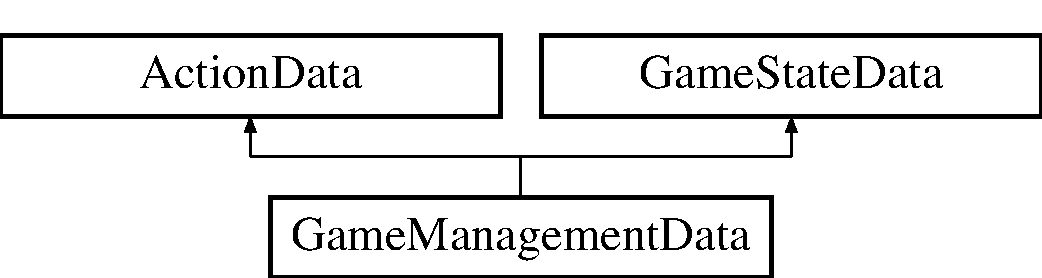
\includegraphics[height=2.000000cm]{classGameManagementData}
\end{center}
\end{figure}
\subsection*{Public Member Functions}
\begin{DoxyCompactItemize}
\item 
\hyperlink{classGameManagementData_a62ed683d4e02da56bda0507892a72041}{Game\-Management\-Data} ()
\begin{DoxyCompactList}\small\item\em Constructor. \end{DoxyCompactList}\item 
virtual void \hyperlink{classGameManagementData_ae49afd739e313caf0b5cd3799be1b125}{reset\-Actions\-Info} ()
\begin{DoxyCompactList}\small\item\em Virtual void function, look to child for defenition. \end{DoxyCompactList}\item 
virtual const \hyperlink{structactions__info}{actions\-\_\-info} \& \hyperlink{classGameManagementData_afa213f0d90a9d0878fae317457f5e851}{give\-Action\-Info} () const 
\begin{DoxyCompactList}\small\item\em Returns the action data container held by the class. \end{DoxyCompactList}\item 
virtual void \hyperlink{classGameManagementData_a2e9acf1ddddabee775dc106b478aa2e2}{reset\-Turret\-Fire} ()
\begin{DoxyCompactList}\small\item\em Reset the firing condition of the game Turrets. \end{DoxyCompactList}\item 
virtual void \hyperlink{classGameManagementData_aa3e5f9aaa99a44c4518933ad75b7ccd6}{set\-Turret\-Fire} ()
\begin{DoxyCompactList}\small\item\em Enable the firing conditon of the game Turrets. \end{DoxyCompactList}\item 
virtual void \hyperlink{classGameManagementData_a4ad4fccb78261b8299142db3185828e3}{move\-Forward\-P1} ()
\begin{DoxyCompactList}\small\item\em Set Player1 to move forward. \end{DoxyCompactList}\item 
virtual void \hyperlink{classGameManagementData_ab023b818d0ffc740fc5574654ff89cfa}{move\-Backward\-P1} ()
\begin{DoxyCompactList}\small\item\em Set player2 to move forward. \end{DoxyCompactList}\item 
virtual void \hyperlink{classGameManagementData_afe92b173c32488f148fc7a2fa3ac0388}{rotate\-Left\-P1} ()
\begin{DoxyCompactList}\small\item\em Set player1 to rotate left. \end{DoxyCompactList}\item 
virtual void \hyperlink{classGameManagementData_a933b945bef3e7b15306ed361f611ec2d}{rotate\-Right\-P1} ()
\begin{DoxyCompactList}\small\item\em Set player1 to rotate right. \end{DoxyCompactList}\item 
virtual void \hyperlink{classGameManagementData_ab434e39574c0511a37bd5799607dc782}{move\-Forward\-P2} ()
\begin{DoxyCompactList}\small\item\em Set player2 to move forward. \end{DoxyCompactList}\item 
virtual void \hyperlink{classGameManagementData_a130c7b68c41bfcc92bae027f5db11e68}{move\-Backward\-P2} ()
\begin{DoxyCompactList}\small\item\em Set player 2 to move backward. \end{DoxyCompactList}\item 
virtual void \hyperlink{classGameManagementData_a7b6ba982e678159bd687243facce3ab2}{rotate\-Left\-P2} ()
\begin{DoxyCompactList}\small\item\em Set player 2 to rotate left. \end{DoxyCompactList}\item 
virtual void \hyperlink{classGameManagementData_a93b5d21e2b4e347e8d7051885aab2bb2}{rotate\-Right\-P2} ()
\begin{DoxyCompactList}\small\item\em Set player 2 to rotate right. \end{DoxyCompactList}\item 
virtual void \hyperlink{classGameManagementData_af31200e3fa7302496f48d81ad3934ace}{missile\-Fired\-P1} ()
\begin{DoxyCompactList}\small\item\em Set missile for player 1 fired. \end{DoxyCompactList}\item 
virtual void \hyperlink{classGameManagementData_ae55ccfb644fc58de62c42779dbf710c4}{missile\-Fired\-P2} ()
\begin{DoxyCompactList}\small\item\em Set missile for player 2 fired. \end{DoxyCompactList}\item 
virtual void \hyperlink{classGameManagementData_a5450f20ab4ad8d8f81c4d673ea72bfc2}{mine\-Laid\-P1} ()
\begin{DoxyCompactList}\small\item\em Set mine laid for player 1. \end{DoxyCompactList}\item 
virtual void \hyperlink{classGameManagementData_a794b882a00b5c979e59590db0c452828}{mine\-Laid\-P2} ()
\begin{DoxyCompactList}\small\item\em Set mine laid for player 2. \end{DoxyCompactList}\item 
virtual void \hyperlink{classGameManagementData_a82c3d16a50fb6e79a3b9aaca2272d000}{reset\-P1\-Attack} ()
\begin{DoxyCompactList}\small\item\em Restt player1 attack state. \end{DoxyCompactList}\item 
virtual void \hyperlink{classGameManagementData_a3434062fcb5872de24787b2cfa49b605}{reset\-P2\-Attack} ()
\begin{DoxyCompactList}\small\item\em Reset player2 attack state. \end{DoxyCompactList}\item 
virtual const int \hyperlink{classGameManagementData_a2738ec4d85bdb87f957d21e8a314e502}{get\-P1\-Score} ()
\begin{DoxyCompactList}\small\item\em Getter for p1 score. \end{DoxyCompactList}\item 
virtual const int \hyperlink{classGameManagementData_ad1d991be2ab8b8f814ef6898dd887d15}{get\-P2\-Score} ()
\begin{DoxyCompactList}\small\item\em Getter for p2 score. \end{DoxyCompactList}\item 
virtual void \hyperlink{classGameManagementData_a7d574170fe76a837c05372c8c52eed63}{increase\-P1\-Score} ()
\begin{DoxyCompactList}\small\item\em Increment p1 score by 1. \end{DoxyCompactList}\item 
virtual void \hyperlink{classGameManagementData_a9a7a124ef719be6f9d45c4ec231e7774}{increase\-P2\-Score} ()
\begin{DoxyCompactList}\small\item\em Increment p2 score by 1. \end{DoxyCompactList}\item 
virtual void \hyperlink{classGameManagementData_a1df14e6642056790f6677cbd779c6815}{set\-P1\-Respawn} ()
\begin{DoxyCompactList}\small\item\em Set p1 to respawn. \end{DoxyCompactList}\item 
virtual void \hyperlink{classGameManagementData_a31113c80e1caa2604c98db63d565641a}{set\-P2\-Respawn} ()
\begin{DoxyCompactList}\small\item\em Set p2 to respawn. \end{DoxyCompactList}\item 
virtual void \hyperlink{classGameManagementData_a66c80fd2795e9e95fe47ad5a77263a9b}{disable\-P1\-Respawn} ()
\begin{DoxyCompactList}\small\item\em Disable p1 to respawn. \end{DoxyCompactList}\item 
virtual void \hyperlink{classGameManagementData_a2bcc4361d645773587a722755f53cf29}{disable\-P2\-Respawn} ()
\begin{DoxyCompactList}\small\item\em Disable p2 to respawn. \end{DoxyCompactList}\item 
virtual const bool \hyperlink{classGameManagementData_a2abb452bd5ecd1f8d09b76dc1f909260}{is\-P1\-Respawn} ()
\begin{DoxyCompactList}\small\item\em Check if p1 is respawnable. \end{DoxyCompactList}\item 
virtual const bool \hyperlink{classGameManagementData_a3b94efaf212d65515c1c511a17636b5f}{is\-P2\-Respawn} ()
\begin{DoxyCompactList}\small\item\em Check if p2 is respawnable. \end{DoxyCompactList}\item 
virtual const bool \hyperlink{classGameManagementData_ac8d6deb9285fe8e5205f9984b0a2622d}{is\-Game\-Finished} ()
\begin{DoxyCompactList}\small\item\em Check if \hyperlink{classGame}{Game} is in a finished state. \end{DoxyCompactList}\item 
virtual void \hyperlink{classGameManagementData_afef95ac9618619ca6ec29277fd04c361}{set\-Game\-Finished} ()
\begin{DoxyCompactList}\small\item\em Set game in a finishe state. \end{DoxyCompactList}\item 
virtual void \hyperlink{classGameManagementData_ae3ed7d9a9cbed2222ad34c52a4bcfd5c}{set\-Game\-Time} (const float game\-\_\-time)
\begin{DoxyCompactList}\small\item\em Set the game time. \end{DoxyCompactList}\item 
virtual const float \hyperlink{classGameManagementData_aa507f9e395464888ad9dc66a90b1bbc3}{get\-Game\-Time} ()
\begin{DoxyCompactList}\small\item\em Retrieve the game time for draw manager. \end{DoxyCompactList}\item 
virtual \hyperlink{classGameManagementData_aa665bdaa6c75dcf11c5e24bc6173d07b}{$\sim$\-Game\-Management\-Data} ()
\begin{DoxyCompactList}\small\item\em Destructor. \end{DoxyCompactList}\end{DoxyCompactItemize}
\subsection*{Private Attributes}
\begin{DoxyCompactItemize}
\item 
\hyperlink{structactions__info}{actions\-\_\-info} \hyperlink{classGameManagementData_a2e8b33eea89438fece399848770c1b7e}{\-\_\-game\-\_\-actions}
\item 
int \hyperlink{classGameManagementData_a76ffd3ea3cbcf32cd0c8e11e65e1932e}{\-\_\-p1\-\_\-score}
\item 
int \hyperlink{classGameManagementData_a40cf0c43247ade13defa7438f552e8ae}{\-\_\-p2\-\_\-score}
\item 
bool \hyperlink{classGameManagementData_aa7c7d0776da7b60a01188141ac32cdfa}{\-\_\-p1\-\_\-respawn}
\item 
bool \hyperlink{classGameManagementData_a6515f5db7d5f36b3fd7175ed35109ab1}{\-\_\-p2\-\_\-respawn}
\item 
bool \hyperlink{classGameManagementData_a9b7ff181d9a1df074a9d2ff0dea435df}{\-\_\-game\-\_\-state}
\item 
float \hyperlink{classGameManagementData_aab72e0664819cafeaa49f2fc2ec73a1a}{\-\_\-game\-\_\-time}
\end{DoxyCompactItemize}


\subsection{Detailed Description}
Implementation for the \hyperlink{classGameManagementData}{Game\-Management\-Data} Class. 

\hyperlink{classGameManagementData}{Game\-Management\-Data} serves as a dynamic data container which is passed around during the game management cycle. It holds basic getter and setter functions which are visible to only certain managers at specific times. 

Definition at line 17 of file Game\-Management\-Data.\-h.



\subsection{Constructor \& Destructor Documentation}
\hypertarget{classGameManagementData_a62ed683d4e02da56bda0507892a72041}{\index{Game\-Management\-Data@{Game\-Management\-Data}!Game\-Management\-Data@{Game\-Management\-Data}}
\index{Game\-Management\-Data@{Game\-Management\-Data}!GameManagementData@{Game\-Management\-Data}}
\subsubsection[{Game\-Management\-Data}]{\setlength{\rightskip}{0pt plus 5cm}Game\-Management\-Data\-::\-Game\-Management\-Data (
\begin{DoxyParamCaption}
{}
\end{DoxyParamCaption}
)}}\label{classGameManagementData_a62ed683d4e02da56bda0507892a72041}


Constructor. 

Constructor for \hyperlink{classGameManagementData}{Game\-Management\-Data} object.

Initialises all private data members to a zero state. The reset actions info funcition called during the constructor ensures the struct held by the class is set to zero as well. 

Definition at line 19 of file Game\-Management\-Data.\-cpp.



References reset\-Actions\-Info().


\begin{DoxyCode}
19                                        :
20      \hyperlink{classGameManagementData_a76ffd3ea3cbcf32cd0c8e11e65e1932e}{\_p1\_score}(0),
21      \hyperlink{classGameManagementData_a40cf0c43247ade13defa7438f552e8ae}{\_p2\_score}(0),
22      \hyperlink{classGameManagementData_aab72e0664819cafeaa49f2fc2ec73a1a}{\_game\_time}(0),
23      \hyperlink{classGameManagementData_aa7c7d0776da7b60a01188141ac32cdfa}{\_p1\_respawn}(\textcolor{keyword}{false}),
24      \hyperlink{classGameManagementData_a6515f5db7d5f36b3fd7175ed35109ab1}{\_p2\_respawn}(\textcolor{keyword}{false}),
25      \hyperlink{classGameManagementData_a9b7ff181d9a1df074a9d2ff0dea435df}{\_game\_state}(\textcolor{keyword}{false})
26      \{
27         \hyperlink{classGameManagementData_ae49afd739e313caf0b5cd3799be1b125}{resetActionsInfo}();
28      \}
\end{DoxyCode}
\hypertarget{classGameManagementData_aa665bdaa6c75dcf11c5e24bc6173d07b}{\index{Game\-Management\-Data@{Game\-Management\-Data}!$\sim$\-Game\-Management\-Data@{$\sim$\-Game\-Management\-Data}}
\index{$\sim$\-Game\-Management\-Data@{$\sim$\-Game\-Management\-Data}!GameManagementData@{Game\-Management\-Data}}
\subsubsection[{$\sim$\-Game\-Management\-Data}]{\setlength{\rightskip}{0pt plus 5cm}Game\-Management\-Data\-::$\sim$\-Game\-Management\-Data (
\begin{DoxyParamCaption}
{}
\end{DoxyParamCaption}
)\hspace{0.3cm}{\ttfamily [virtual]}}}\label{classGameManagementData_aa665bdaa6c75dcf11c5e24bc6173d07b}


Destructor. 



Definition at line 320 of file Game\-Management\-Data.\-cpp.


\begin{DoxyCode}
321 \{
322 
323 \}
\end{DoxyCode}


\subsection{Member Function Documentation}
\hypertarget{classGameManagementData_a66c80fd2795e9e95fe47ad5a77263a9b}{\index{Game\-Management\-Data@{Game\-Management\-Data}!disable\-P1\-Respawn@{disable\-P1\-Respawn}}
\index{disable\-P1\-Respawn@{disable\-P1\-Respawn}!GameManagementData@{Game\-Management\-Data}}
\subsubsection[{disable\-P1\-Respawn}]{\setlength{\rightskip}{0pt plus 5cm}void Game\-Management\-Data\-::disable\-P1\-Respawn (
\begin{DoxyParamCaption}
{}
\end{DoxyParamCaption}
)\hspace{0.3cm}{\ttfamily [virtual]}}}\label{classGameManagementData_a66c80fd2795e9e95fe47ad5a77263a9b}


Disable p1 to respawn. 

Disallow p1 to respwan again.

This function stops the \hyperlink{classGame}{Game} object from creating another tank player while it is alive it has been destroyed 

Implements \hyperlink{classGameStateData_a0599750aaaa0d272ba8e073d84b0e82b}{Game\-State\-Data}.



Definition at line 254 of file Game\-Management\-Data.\-cpp.



References \-\_\-p1\-\_\-respawn.



Referenced by Game\-::manage\-Respawns().


\begin{DoxyCode}
255 \{
256     \hyperlink{classGameManagementData_aa7c7d0776da7b60a01188141ac32cdfa}{\_p1\_respawn} = \textcolor{keyword}{false};
257 \}
\end{DoxyCode}
\hypertarget{classGameManagementData_a2bcc4361d645773587a722755f53cf29}{\index{Game\-Management\-Data@{Game\-Management\-Data}!disable\-P2\-Respawn@{disable\-P2\-Respawn}}
\index{disable\-P2\-Respawn@{disable\-P2\-Respawn}!GameManagementData@{Game\-Management\-Data}}
\subsubsection[{disable\-P2\-Respawn}]{\setlength{\rightskip}{0pt plus 5cm}void Game\-Management\-Data\-::disable\-P2\-Respawn (
\begin{DoxyParamCaption}
{}
\end{DoxyParamCaption}
)\hspace{0.3cm}{\ttfamily [virtual]}}}\label{classGameManagementData_a2bcc4361d645773587a722755f53cf29}


Disable p2 to respawn. 

Disallow p2 to respwan again.

This function stops the \hyperlink{classGame}{Game} object from creating another tank player while it is alive it has been destroyed 

Implements \hyperlink{classGameStateData_a5886e86d10a106cf490eaa2433f3e3ea}{Game\-State\-Data}.



Definition at line 263 of file Game\-Management\-Data.\-cpp.



References \-\_\-p2\-\_\-respawn.



Referenced by Game\-::manage\-Respawns().


\begin{DoxyCode}
264 \{
265     \hyperlink{classGameManagementData_a6515f5db7d5f36b3fd7175ed35109ab1}{\_p2\_respawn} = \textcolor{keyword}{false};
266 \}
\end{DoxyCode}
\hypertarget{classGameManagementData_aa507f9e395464888ad9dc66a90b1bbc3}{\index{Game\-Management\-Data@{Game\-Management\-Data}!get\-Game\-Time@{get\-Game\-Time}}
\index{get\-Game\-Time@{get\-Game\-Time}!GameManagementData@{Game\-Management\-Data}}
\subsubsection[{get\-Game\-Time}]{\setlength{\rightskip}{0pt plus 5cm}const float Game\-Management\-Data\-::get\-Game\-Time (
\begin{DoxyParamCaption}
{}
\end{DoxyParamCaption}
)\hspace{0.3cm}{\ttfamily [virtual]}}}\label{classGameManagementData_aa507f9e395464888ad9dc66a90b1bbc3}


Retrieve the game time for draw manager. 

Function to fetch the current game time.

Returns the value of the current game timer within \hyperlink{classGameStateManager}{Game\-State\-Manager} 

Implements \hyperlink{classGameStateData_a0cb5cf167da9dd1929c719778c5d3506}{Game\-State\-Data}.



Definition at line 315 of file Game\-Management\-Data.\-cpp.



References \-\_\-game\-\_\-time.


\begin{DoxyCode}
316 \{
317     \textcolor{keywordflow}{return} \hyperlink{classGameManagementData_aab72e0664819cafeaa49f2fc2ec73a1a}{\_game\_time};
318 \}
\end{DoxyCode}
\hypertarget{classGameManagementData_a2738ec4d85bdb87f957d21e8a314e502}{\index{Game\-Management\-Data@{Game\-Management\-Data}!get\-P1\-Score@{get\-P1\-Score}}
\index{get\-P1\-Score@{get\-P1\-Score}!GameManagementData@{Game\-Management\-Data}}
\subsubsection[{get\-P1\-Score}]{\setlength{\rightskip}{0pt plus 5cm}const int Game\-Management\-Data\-::get\-P1\-Score (
\begin{DoxyParamCaption}
{}
\end{DoxyParamCaption}
)\hspace{0.3cm}{\ttfamily [virtual]}}}\label{classGameManagementData_a2738ec4d85bdb87f957d21e8a314e502}


Getter for p1 score. 

Retrieve p1 score.

This is a simple getter method 

Implements \hyperlink{classGameStateData_ac4dbf8f19eb4abae6c6e674e1f0ad473}{Game\-State\-Data}.



Definition at line 200 of file Game\-Management\-Data.\-cpp.



References \-\_\-p1\-\_\-score.



Referenced by T\-E\-S\-T().


\begin{DoxyCode}
201 \{
202     \textcolor{keywordflow}{return} \hyperlink{classGameManagementData_a76ffd3ea3cbcf32cd0c8e11e65e1932e}{\_p1\_score};
203 \}
\end{DoxyCode}
\hypertarget{classGameManagementData_ad1d991be2ab8b8f814ef6898dd887d15}{\index{Game\-Management\-Data@{Game\-Management\-Data}!get\-P2\-Score@{get\-P2\-Score}}
\index{get\-P2\-Score@{get\-P2\-Score}!GameManagementData@{Game\-Management\-Data}}
\subsubsection[{get\-P2\-Score}]{\setlength{\rightskip}{0pt plus 5cm}const int Game\-Management\-Data\-::get\-P2\-Score (
\begin{DoxyParamCaption}
{}
\end{DoxyParamCaption}
)\hspace{0.3cm}{\ttfamily [virtual]}}}\label{classGameManagementData_ad1d991be2ab8b8f814ef6898dd887d15}


Getter for p2 score. 

Retrieve p2 score.

This is a simple getter method 

Implements \hyperlink{classGameStateData_a024affaa547433a0feca091d2bc516b6}{Game\-State\-Data}.



Definition at line 208 of file Game\-Management\-Data.\-cpp.



References \-\_\-p2\-\_\-score.



Referenced by T\-E\-S\-T().


\begin{DoxyCode}
209 \{
210     \textcolor{keywordflow}{return} \hyperlink{classGameManagementData_a40cf0c43247ade13defa7438f552e8ae}{\_p2\_score};
211 \}
\end{DoxyCode}
\hypertarget{classGameManagementData_afa213f0d90a9d0878fae317457f5e851}{\index{Game\-Management\-Data@{Game\-Management\-Data}!give\-Action\-Info@{give\-Action\-Info}}
\index{give\-Action\-Info@{give\-Action\-Info}!GameManagementData@{Game\-Management\-Data}}
\subsubsection[{give\-Action\-Info}]{\setlength{\rightskip}{0pt plus 5cm}const {\bf actions\-\_\-info} \& Game\-Management\-Data\-::give\-Action\-Info (
\begin{DoxyParamCaption}
{}
\end{DoxyParamCaption}
) const\hspace{0.3cm}{\ttfamily [virtual]}}}\label{classGameManagementData_afa213f0d90a9d0878fae317457f5e851}


Returns the action data container held by the class. 

Getter for the \hyperlink{structactions__info}{actions\-\_\-info} object.

This retrieves the current version of the \hyperlink{structactions__info}{actions\-\_\-info} container \begin{DoxyReturn}{Returns}
\hyperlink{structactions__info}{actions\-\_\-info} 
\end{DoxyReturn}


Implements \hyperlink{classActionData_ab2f5b210968c91a01ed1439904b3ffee}{Action\-Data}.



Definition at line 50 of file Game\-Management\-Data.\-cpp.



References \-\_\-game\-\_\-actions.



Referenced by Game\-::add\-New\-World\-Entity(), and T\-E\-S\-T().


\begin{DoxyCode}
51 \{
52     \textcolor{keywordflow}{return} \hyperlink{classGameManagementData_a2e8b33eea89438fece399848770c1b7e}{\_game\_actions};
53 \}
\end{DoxyCode}
\hypertarget{classGameManagementData_a7d574170fe76a837c05372c8c52eed63}{\index{Game\-Management\-Data@{Game\-Management\-Data}!increase\-P1\-Score@{increase\-P1\-Score}}
\index{increase\-P1\-Score@{increase\-P1\-Score}!GameManagementData@{Game\-Management\-Data}}
\subsubsection[{increase\-P1\-Score}]{\setlength{\rightskip}{0pt plus 5cm}void Game\-Management\-Data\-::increase\-P1\-Score (
\begin{DoxyParamCaption}
{}
\end{DoxyParamCaption}
)\hspace{0.3cm}{\ttfamily [virtual]}}}\label{classGameManagementData_a7d574170fe76a837c05372c8c52eed63}


Increment p1 score by 1. 

Increment p1 score.

This increments p1's score by one point 

Implements \hyperlink{classGameStateData_a28ec2cf2d7dd89bab394b611a83e7d4c}{Game\-State\-Data}.



Definition at line 216 of file Game\-Management\-Data.\-cpp.



References \-\_\-p1\-\_\-respawn, and \-\_\-p1\-\_\-score.


\begin{DoxyCode}
217 \{
218     \hyperlink{classGameManagementData_a76ffd3ea3cbcf32cd0c8e11e65e1932e}{\_p1\_score}++;
219     \hyperlink{classGameManagementData_aa7c7d0776da7b60a01188141ac32cdfa}{\_p1\_respawn} = \textcolor{keyword}{true};
220 \}
\end{DoxyCode}
\hypertarget{classGameManagementData_a9a7a124ef719be6f9d45c4ec231e7774}{\index{Game\-Management\-Data@{Game\-Management\-Data}!increase\-P2\-Score@{increase\-P2\-Score}}
\index{increase\-P2\-Score@{increase\-P2\-Score}!GameManagementData@{Game\-Management\-Data}}
\subsubsection[{increase\-P2\-Score}]{\setlength{\rightskip}{0pt plus 5cm}void Game\-Management\-Data\-::increase\-P2\-Score (
\begin{DoxyParamCaption}
{}
\end{DoxyParamCaption}
)\hspace{0.3cm}{\ttfamily [virtual]}}}\label{classGameManagementData_a9a7a124ef719be6f9d45c4ec231e7774}


Increment p2 score by 1. 

Increment p2 score.

This increments p2's score by one point 

Implements \hyperlink{classGameStateData_a8b2470bafedd2c51cdc32199ae004b13}{Game\-State\-Data}.



Definition at line 226 of file Game\-Management\-Data.\-cpp.



References \-\_\-p2\-\_\-respawn, and \-\_\-p2\-\_\-score.


\begin{DoxyCode}
227 \{
228     \hyperlink{classGameManagementData_a40cf0c43247ade13defa7438f552e8ae}{\_p2\_score}++;
229     \hyperlink{classGameManagementData_a6515f5db7d5f36b3fd7175ed35109ab1}{\_p2\_respawn} = \textcolor{keyword}{true};
230 \}
\end{DoxyCode}
\hypertarget{classGameManagementData_ac8d6deb9285fe8e5205f9984b0a2622d}{\index{Game\-Management\-Data@{Game\-Management\-Data}!is\-Game\-Finished@{is\-Game\-Finished}}
\index{is\-Game\-Finished@{is\-Game\-Finished}!GameManagementData@{Game\-Management\-Data}}
\subsubsection[{is\-Game\-Finished}]{\setlength{\rightskip}{0pt plus 5cm}const bool Game\-Management\-Data\-::is\-Game\-Finished (
\begin{DoxyParamCaption}
{}
\end{DoxyParamCaption}
)\hspace{0.3cm}{\ttfamily [virtual]}}}\label{classGameManagementData_ac8d6deb9285fe8e5205f9984b0a2622d}


Check if \hyperlink{classGame}{Game} is in a finished state. 

Check boolean state of the game.

This function will return a true result after 2 minutes of the game running. \begin{DoxyReturn}{Returns}
bool 
\end{DoxyReturn}


Implements \hyperlink{classGameStateData_a96b7a0057780d2fac25569019804428e}{Game\-State\-Data}.



Definition at line 290 of file Game\-Management\-Data.\-cpp.



References \-\_\-game\-\_\-state.



Referenced by Game\-::run\-World().


\begin{DoxyCode}
291 \{
292     \textcolor{keywordflow}{return} \hyperlink{classGameManagementData_a9b7ff181d9a1df074a9d2ff0dea435df}{\_game\_state};
293 \}
\end{DoxyCode}
\hypertarget{classGameManagementData_a2abb452bd5ecd1f8d09b76dc1f909260}{\index{Game\-Management\-Data@{Game\-Management\-Data}!is\-P1\-Respawn@{is\-P1\-Respawn}}
\index{is\-P1\-Respawn@{is\-P1\-Respawn}!GameManagementData@{Game\-Management\-Data}}
\subsubsection[{is\-P1\-Respawn}]{\setlength{\rightskip}{0pt plus 5cm}const bool Game\-Management\-Data\-::is\-P1\-Respawn (
\begin{DoxyParamCaption}
{}
\end{DoxyParamCaption}
)\hspace{0.3cm}{\ttfamily [virtual]}}}\label{classGameManagementData_a2abb452bd5ecd1f8d09b76dc1f909260}


Check if p1 is respawnable. 

Check boolean state of the respawn condition.

Check for changes to see if p1 needs to be respawned 

Implements \hyperlink{classGameStateData_a1893643563270c9ca0552761d0da1085}{Game\-State\-Data}.



Definition at line 272 of file Game\-Management\-Data.\-cpp.



References \-\_\-p1\-\_\-respawn.



Referenced by Game\-::manage\-Respawns().


\begin{DoxyCode}
273 \{
274     \textcolor{keywordflow}{return} \hyperlink{classGameManagementData_aa7c7d0776da7b60a01188141ac32cdfa}{\_p1\_respawn};
275 \}
\end{DoxyCode}
\hypertarget{classGameManagementData_a3b94efaf212d65515c1c511a17636b5f}{\index{Game\-Management\-Data@{Game\-Management\-Data}!is\-P2\-Respawn@{is\-P2\-Respawn}}
\index{is\-P2\-Respawn@{is\-P2\-Respawn}!GameManagementData@{Game\-Management\-Data}}
\subsubsection[{is\-P2\-Respawn}]{\setlength{\rightskip}{0pt plus 5cm}const bool Game\-Management\-Data\-::is\-P2\-Respawn (
\begin{DoxyParamCaption}
{}
\end{DoxyParamCaption}
)\hspace{0.3cm}{\ttfamily [virtual]}}}\label{classGameManagementData_a3b94efaf212d65515c1c511a17636b5f}


Check if p2 is respawnable. 

Check boolean state of the respawn condition.

Check for changes to see if p2 needs to be respawned 

Implements \hyperlink{classGameStateData_af65fd6264b007c67e17ffa23e1b91cdb}{Game\-State\-Data}.



Definition at line 280 of file Game\-Management\-Data.\-cpp.



References \-\_\-p2\-\_\-respawn.



Referenced by Game\-::manage\-Respawns().


\begin{DoxyCode}
281 \{
282     \textcolor{keywordflow}{return} \hyperlink{classGameManagementData_a6515f5db7d5f36b3fd7175ed35109ab1}{\_p2\_respawn};
283 \}
\end{DoxyCode}
\hypertarget{classGameManagementData_a5450f20ab4ad8d8f81c4d673ea72bfc2}{\index{Game\-Management\-Data@{Game\-Management\-Data}!mine\-Laid\-P1@{mine\-Laid\-P1}}
\index{mine\-Laid\-P1@{mine\-Laid\-P1}!GameManagementData@{Game\-Management\-Data}}
\subsubsection[{mine\-Laid\-P1}]{\setlength{\rightskip}{0pt plus 5cm}void Game\-Management\-Data\-::mine\-Laid\-P1 (
\begin{DoxyParamCaption}
{}
\end{DoxyParamCaption}
)\hspace{0.3cm}{\ttfamily [virtual]}}}\label{classGameManagementData_a5450f20ab4ad8d8f81c4d673ea72bfc2}


Set mine laid for player 1. 

Sets condition for p1 to lay a mine.

This is a simple setter for p1 to lay a mine 

Implements \hyperlink{classActionData_a8abc4e84c4e6d676010c7e2497278312}{Action\-Data}.



Definition at line 166 of file Game\-Management\-Data.\-cpp.



References \-\_\-game\-\_\-actions, actions\-\_\-info\-::attack\-\_\-1, actions\-\_\-info\-::change\-\_\-1, and lay\-\_\-mine.



Referenced by T\-E\-S\-T().


\begin{DoxyCode}
167 \{
168     \hyperlink{classGameManagementData_a2e8b33eea89438fece399848770c1b7e}{\_game\_actions}.\hyperlink{structactions__info_a69ac673533838f973f09492a12516816}{change\_1} = \textcolor{keyword}{true};
169     \hyperlink{classGameManagementData_a2e8b33eea89438fece399848770c1b7e}{\_game\_actions}.\hyperlink{structactions__info_a722a3805cc06ba6e5f9627b942f9bbf2}{attack\_1} = \hyperlink{Structures_8h_abf3d9daa4559fb2f9e16fc1836fead1baed59f3b92945ae37d3f2f4e7472acacc}{lay\_mine};
170 \}
\end{DoxyCode}
\hypertarget{classGameManagementData_a794b882a00b5c979e59590db0c452828}{\index{Game\-Management\-Data@{Game\-Management\-Data}!mine\-Laid\-P2@{mine\-Laid\-P2}}
\index{mine\-Laid\-P2@{mine\-Laid\-P2}!GameManagementData@{Game\-Management\-Data}}
\subsubsection[{mine\-Laid\-P2}]{\setlength{\rightskip}{0pt plus 5cm}void Game\-Management\-Data\-::mine\-Laid\-P2 (
\begin{DoxyParamCaption}
{}
\end{DoxyParamCaption}
)\hspace{0.3cm}{\ttfamily [virtual]}}}\label{classGameManagementData_a794b882a00b5c979e59590db0c452828}


Set mine laid for player 2. 

Sets condition for p2 to lay a mine.

This is a simple setter for p2 to lay a mine 

Implements \hyperlink{classActionData_a71c04f577d3c06aa45b7c43d935ca567}{Action\-Data}.



Definition at line 175 of file Game\-Management\-Data.\-cpp.



References \-\_\-game\-\_\-actions, actions\-\_\-info\-::attack\-\_\-2, actions\-\_\-info\-::change\-\_\-2, and lay\-\_\-mine.



Referenced by T\-E\-S\-T().


\begin{DoxyCode}
176 \{
177     \hyperlink{classGameManagementData_a2e8b33eea89438fece399848770c1b7e}{\_game\_actions}.\hyperlink{structactions__info_a0f20d9c244d92a71dad9cf8ce10cd2f2}{change\_2} = \textcolor{keyword}{true};
178     \hyperlink{classGameManagementData_a2e8b33eea89438fece399848770c1b7e}{\_game\_actions}.\hyperlink{structactions__info_a9bfb93ce33b8969b45fa72a12b89be89}{attack\_2} = \hyperlink{Structures_8h_abf3d9daa4559fb2f9e16fc1836fead1baed59f3b92945ae37d3f2f4e7472acacc}{lay\_mine};
179 \}
\end{DoxyCode}
\hypertarget{classGameManagementData_af31200e3fa7302496f48d81ad3934ace}{\index{Game\-Management\-Data@{Game\-Management\-Data}!missile\-Fired\-P1@{missile\-Fired\-P1}}
\index{missile\-Fired\-P1@{missile\-Fired\-P1}!GameManagementData@{Game\-Management\-Data}}
\subsubsection[{missile\-Fired\-P1}]{\setlength{\rightskip}{0pt plus 5cm}void Game\-Management\-Data\-::missile\-Fired\-P1 (
\begin{DoxyParamCaption}
{}
\end{DoxyParamCaption}
)\hspace{0.3cm}{\ttfamily [virtual]}}}\label{classGameManagementData_af31200e3fa7302496f48d81ad3934ace}


Set missile for player 1 fired. 

Sets condition for p1 to fire missile.

This is a simple setter for p1 missile firing 

Implements \hyperlink{classActionData_aeb7f1219ff0bf0cc81fee1d669317cdb}{Action\-Data}.



Definition at line 148 of file Game\-Management\-Data.\-cpp.



References \-\_\-game\-\_\-actions, actions\-\_\-info\-::attack\-\_\-1, actions\-\_\-info\-::change\-\_\-1, and fire\-\_\-missile.



Referenced by T\-E\-S\-T().


\begin{DoxyCode}
149 \{
150     \hyperlink{classGameManagementData_a2e8b33eea89438fece399848770c1b7e}{\_game\_actions}.\hyperlink{structactions__info_a69ac673533838f973f09492a12516816}{change\_1} = \textcolor{keyword}{true};
151     \hyperlink{classGameManagementData_a2e8b33eea89438fece399848770c1b7e}{\_game\_actions}.\hyperlink{structactions__info_a722a3805cc06ba6e5f9627b942f9bbf2}{attack\_1} = \hyperlink{Structures_8h_abf3d9daa4559fb2f9e16fc1836fead1badfc8afb4acc9eae75dcfdde515861288}{fire\_missile};
152 \}
\end{DoxyCode}
\hypertarget{classGameManagementData_ae55ccfb644fc58de62c42779dbf710c4}{\index{Game\-Management\-Data@{Game\-Management\-Data}!missile\-Fired\-P2@{missile\-Fired\-P2}}
\index{missile\-Fired\-P2@{missile\-Fired\-P2}!GameManagementData@{Game\-Management\-Data}}
\subsubsection[{missile\-Fired\-P2}]{\setlength{\rightskip}{0pt plus 5cm}void Game\-Management\-Data\-::missile\-Fired\-P2 (
\begin{DoxyParamCaption}
{}
\end{DoxyParamCaption}
)\hspace{0.3cm}{\ttfamily [virtual]}}}\label{classGameManagementData_ae55ccfb644fc58de62c42779dbf710c4}


Set missile for player 2 fired. 

Sets condition for p2 to fire missile.

This is a simple setter for p2 missile firing 

Implements \hyperlink{classActionData_a5a2d45d0fc03daf8edaacd6a9757fafd}{Action\-Data}.



Definition at line 157 of file Game\-Management\-Data.\-cpp.



References \-\_\-game\-\_\-actions, actions\-\_\-info\-::attack\-\_\-2, actions\-\_\-info\-::change\-\_\-2, and fire\-\_\-missile.



Referenced by T\-E\-S\-T().


\begin{DoxyCode}
158 \{
159     \hyperlink{classGameManagementData_a2e8b33eea89438fece399848770c1b7e}{\_game\_actions}.\hyperlink{structactions__info_a0f20d9c244d92a71dad9cf8ce10cd2f2}{change\_2} = \textcolor{keyword}{true};
160     \hyperlink{classGameManagementData_a2e8b33eea89438fece399848770c1b7e}{\_game\_actions}.\hyperlink{structactions__info_a9bfb93ce33b8969b45fa72a12b89be89}{attack\_2} = \hyperlink{Structures_8h_abf3d9daa4559fb2f9e16fc1836fead1badfc8afb4acc9eae75dcfdde515861288}{fire\_missile};
161 \}
\end{DoxyCode}
\hypertarget{classGameManagementData_ab023b818d0ffc740fc5574654ff89cfa}{\index{Game\-Management\-Data@{Game\-Management\-Data}!move\-Backward\-P1@{move\-Backward\-P1}}
\index{move\-Backward\-P1@{move\-Backward\-P1}!GameManagementData@{Game\-Management\-Data}}
\subsubsection[{move\-Backward\-P1}]{\setlength{\rightskip}{0pt plus 5cm}void Game\-Management\-Data\-::move\-Backward\-P1 (
\begin{DoxyParamCaption}
{}
\end{DoxyParamCaption}
)\hspace{0.3cm}{\ttfamily [virtual]}}}\label{classGameManagementData_ab023b818d0ffc740fc5574654ff89cfa}


Set player2 to move forward. 

Sets p1 to move backward.

This is a simple setter for p1 backward movement 

Implements \hyperlink{classActionData_a711265f479e845086896c42d1e906c57}{Action\-Data}.



Definition at line 85 of file Game\-Management\-Data.\-cpp.



References \-\_\-game\-\_\-actions, actions\-\_\-info\-::change\-\_\-1, actions\-\_\-info\-::move\-\_\-1, and reverse.


\begin{DoxyCode}
86 \{
87     \hyperlink{classGameManagementData_a2e8b33eea89438fece399848770c1b7e}{\_game\_actions}.\hyperlink{structactions__info_a69ac673533838f973f09492a12516816}{change\_1} = \textcolor{keyword}{true};
88     \hyperlink{classGameManagementData_a2e8b33eea89438fece399848770c1b7e}{\_game\_actions}.\hyperlink{structactions__info_a5cb853144009b2bfb7e58c7bf43e2a42}{move\_1} = \hyperlink{Structures_8h_abf3d9daa4559fb2f9e16fc1836fead1ba5a40f8ecbed801e00fddb306fc5666f0}{reverse};
89 \}
\end{DoxyCode}
\hypertarget{classGameManagementData_a130c7b68c41bfcc92bae027f5db11e68}{\index{Game\-Management\-Data@{Game\-Management\-Data}!move\-Backward\-P2@{move\-Backward\-P2}}
\index{move\-Backward\-P2@{move\-Backward\-P2}!GameManagementData@{Game\-Management\-Data}}
\subsubsection[{move\-Backward\-P2}]{\setlength{\rightskip}{0pt plus 5cm}void Game\-Management\-Data\-::move\-Backward\-P2 (
\begin{DoxyParamCaption}
{}
\end{DoxyParamCaption}
)\hspace{0.3cm}{\ttfamily [virtual]}}}\label{classGameManagementData_a130c7b68c41bfcc92bae027f5db11e68}


Set player 2 to move backward. 

Sets p2 to move backward.

This is a simple setter for p2 backward movement 

Implements \hyperlink{classActionData_a9914514aed490cdf131f4a4be4d0f411}{Action\-Data}.



Definition at line 121 of file Game\-Management\-Data.\-cpp.



References \-\_\-game\-\_\-actions, actions\-\_\-info\-::change\-\_\-2, actions\-\_\-info\-::move\-\_\-2, and reverse.


\begin{DoxyCode}
122 \{
123     \hyperlink{classGameManagementData_a2e8b33eea89438fece399848770c1b7e}{\_game\_actions}.\hyperlink{structactions__info_a0f20d9c244d92a71dad9cf8ce10cd2f2}{change\_2} = \textcolor{keyword}{true};
124     \hyperlink{classGameManagementData_a2e8b33eea89438fece399848770c1b7e}{\_game\_actions}.\hyperlink{structactions__info_adf9ed4a9ad4b604295846d06872e0ebf}{move\_2} = \hyperlink{Structures_8h_abf3d9daa4559fb2f9e16fc1836fead1ba5a40f8ecbed801e00fddb306fc5666f0}{reverse};
125 \}
\end{DoxyCode}
\hypertarget{classGameManagementData_a4ad4fccb78261b8299142db3185828e3}{\index{Game\-Management\-Data@{Game\-Management\-Data}!move\-Forward\-P1@{move\-Forward\-P1}}
\index{move\-Forward\-P1@{move\-Forward\-P1}!GameManagementData@{Game\-Management\-Data}}
\subsubsection[{move\-Forward\-P1}]{\setlength{\rightskip}{0pt plus 5cm}void Game\-Management\-Data\-::move\-Forward\-P1 (
\begin{DoxyParamCaption}
{}
\end{DoxyParamCaption}
)\hspace{0.3cm}{\ttfamily [virtual]}}}\label{classGameManagementData_a4ad4fccb78261b8299142db3185828e3}


Set Player1 to move forward. 

Sets p1 to move forward.

This is a simple setter for p1 forward movement 

Implements \hyperlink{classActionData_a002859569085e9868adb7beabd3a2ad8}{Action\-Data}.



Definition at line 76 of file Game\-Management\-Data.\-cpp.



References \-\_\-game\-\_\-actions, actions\-\_\-info\-::change\-\_\-1, forward, and actions\-\_\-info\-::move\-\_\-1.



Referenced by T\-E\-S\-T().


\begin{DoxyCode}
77 \{
78     \hyperlink{classGameManagementData_a2e8b33eea89438fece399848770c1b7e}{\_game\_actions}.\hyperlink{structactions__info_a69ac673533838f973f09492a12516816}{change\_1} = \textcolor{keyword}{true};
79     \hyperlink{classGameManagementData_a2e8b33eea89438fece399848770c1b7e}{\_game\_actions}.\hyperlink{structactions__info_a5cb853144009b2bfb7e58c7bf43e2a42}{move\_1} = \hyperlink{Structures_8h_abf3d9daa4559fb2f9e16fc1836fead1ba726a0af5164861adac8c015a742dcf21}{forward};
80 \}
\end{DoxyCode}
\hypertarget{classGameManagementData_ab434e39574c0511a37bd5799607dc782}{\index{Game\-Management\-Data@{Game\-Management\-Data}!move\-Forward\-P2@{move\-Forward\-P2}}
\index{move\-Forward\-P2@{move\-Forward\-P2}!GameManagementData@{Game\-Management\-Data}}
\subsubsection[{move\-Forward\-P2}]{\setlength{\rightskip}{0pt plus 5cm}void Game\-Management\-Data\-::move\-Forward\-P2 (
\begin{DoxyParamCaption}
{}
\end{DoxyParamCaption}
)\hspace{0.3cm}{\ttfamily [virtual]}}}\label{classGameManagementData_ab434e39574c0511a37bd5799607dc782}


Set player2 to move forward. 

Sets p2 to move forward.

This is a simple setter for p2 forward movement 

Implements \hyperlink{classActionData_a30c547419564c80e3764b620bb1833cc}{Action\-Data}.



Definition at line 112 of file Game\-Management\-Data.\-cpp.



References \-\_\-game\-\_\-actions, actions\-\_\-info\-::change\-\_\-2, forward, and actions\-\_\-info\-::move\-\_\-2.



Referenced by T\-E\-S\-T().


\begin{DoxyCode}
113 \{
114     \hyperlink{classGameManagementData_a2e8b33eea89438fece399848770c1b7e}{\_game\_actions}.\hyperlink{structactions__info_a0f20d9c244d92a71dad9cf8ce10cd2f2}{change\_2} = \textcolor{keyword}{true};
115     \hyperlink{classGameManagementData_a2e8b33eea89438fece399848770c1b7e}{\_game\_actions}.\hyperlink{structactions__info_adf9ed4a9ad4b604295846d06872e0ebf}{move\_2} = \hyperlink{Structures_8h_abf3d9daa4559fb2f9e16fc1836fead1ba726a0af5164861adac8c015a742dcf21}{forward};
116 \}
\end{DoxyCode}
\hypertarget{classGameManagementData_ae49afd739e313caf0b5cd3799be1b125}{\index{Game\-Management\-Data@{Game\-Management\-Data}!reset\-Actions\-Info@{reset\-Actions\-Info}}
\index{reset\-Actions\-Info@{reset\-Actions\-Info}!GameManagementData@{Game\-Management\-Data}}
\subsubsection[{reset\-Actions\-Info}]{\setlength{\rightskip}{0pt plus 5cm}void Game\-Management\-Data\-::reset\-Actions\-Info (
\begin{DoxyParamCaption}
{}
\end{DoxyParamCaption}
)\hspace{0.3cm}{\ttfamily [virtual]}}}\label{classGameManagementData_ae49afd739e313caf0b5cd3799be1b125}


Virtual void function, look to child for defenition. 

Reset The \hyperlink{structactions__info}{actions\-\_\-info} structure values to zero.

All values are reduced from their current state to a default idle state 

Implements \hyperlink{classActionData_aede7cfa65182cda2a2d43df11ccf2183}{Action\-Data}.



Definition at line 34 of file Game\-Management\-Data.\-cpp.



References \-\_\-game\-\_\-actions, actions\-\_\-info\-::attack\-\_\-1, actions\-\_\-info\-::attack\-\_\-2, actions\-\_\-info\-::change\-\_\-1, actions\-\_\-info\-::change\-\_\-2, do\-\_\-nothing, actions\-\_\-info\-::move\-\_\-1, actions\-\_\-info\-::move\-\_\-2, and actions\-\_\-info\-::turret\-\_\-fire.



Referenced by Game\-Management\-Data(), Game\-::run\-World(), and T\-E\-S\-T().


\begin{DoxyCode}
35 \{
36     \hyperlink{classGameManagementData_a2e8b33eea89438fece399848770c1b7e}{\_game\_actions}.\hyperlink{structactions__info_a69ac673533838f973f09492a12516816}{change\_1} = \textcolor{keyword}{false};
37     \hyperlink{classGameManagementData_a2e8b33eea89438fece399848770c1b7e}{\_game\_actions}.\hyperlink{structactions__info_a0f20d9c244d92a71dad9cf8ce10cd2f2}{change\_2} = \textcolor{keyword}{false};
38     \hyperlink{classGameManagementData_a2e8b33eea89438fece399848770c1b7e}{\_game\_actions}.\hyperlink{structactions__info_afd5886948959786f75255fccbc965154}{turret\_fire} = \textcolor{keyword}{false};
39     \hyperlink{classGameManagementData_a2e8b33eea89438fece399848770c1b7e}{\_game\_actions}.\hyperlink{structactions__info_a5cb853144009b2bfb7e58c7bf43e2a42}{move\_1} = \hyperlink{Structures_8h_abf3d9daa4559fb2f9e16fc1836fead1ba562e0b8966ea62e894cd91a30eccfc8a}{do\_nothing};
40     \hyperlink{classGameManagementData_a2e8b33eea89438fece399848770c1b7e}{\_game\_actions}.\hyperlink{structactions__info_adf9ed4a9ad4b604295846d06872e0ebf}{move\_2} = \hyperlink{Structures_8h_abf3d9daa4559fb2f9e16fc1836fead1ba562e0b8966ea62e894cd91a30eccfc8a}{do\_nothing};
41     \hyperlink{classGameManagementData_a2e8b33eea89438fece399848770c1b7e}{\_game\_actions}.\hyperlink{structactions__info_a722a3805cc06ba6e5f9627b942f9bbf2}{attack\_1} = \hyperlink{Structures_8h_abf3d9daa4559fb2f9e16fc1836fead1ba562e0b8966ea62e894cd91a30eccfc8a}{do\_nothing};
42     \hyperlink{classGameManagementData_a2e8b33eea89438fece399848770c1b7e}{\_game\_actions}.\hyperlink{structactions__info_a9bfb93ce33b8969b45fa72a12b89be89}{attack\_2} = \hyperlink{Structures_8h_abf3d9daa4559fb2f9e16fc1836fead1ba562e0b8966ea62e894cd91a30eccfc8a}{do\_nothing};
43 \}
\end{DoxyCode}
\hypertarget{classGameManagementData_a82c3d16a50fb6e79a3b9aaca2272d000}{\index{Game\-Management\-Data@{Game\-Management\-Data}!reset\-P1\-Attack@{reset\-P1\-Attack}}
\index{reset\-P1\-Attack@{reset\-P1\-Attack}!GameManagementData@{Game\-Management\-Data}}
\subsubsection[{reset\-P1\-Attack}]{\setlength{\rightskip}{0pt plus 5cm}void Game\-Management\-Data\-::reset\-P1\-Attack (
\begin{DoxyParamCaption}
{}
\end{DoxyParamCaption}
)\hspace{0.3cm}{\ttfamily [virtual]}}}\label{classGameManagementData_a82c3d16a50fb6e79a3b9aaca2272d000}


Restt player1 attack state. 

This stops p1 from attacking.

P1 cannot fire for the current management cycle 

Implements \hyperlink{classActionData_a12925d051a1cd40bddcb18f0be2c2b01}{Action\-Data}.



Definition at line 184 of file Game\-Management\-Data.\-cpp.



References \-\_\-game\-\_\-actions, actions\-\_\-info\-::attack\-\_\-1, and do\-\_\-nothing.


\begin{DoxyCode}
185 \{
186     \hyperlink{classGameManagementData_a2e8b33eea89438fece399848770c1b7e}{\_game\_actions}.\hyperlink{structactions__info_a722a3805cc06ba6e5f9627b942f9bbf2}{attack\_1} = \hyperlink{Structures_8h_abf3d9daa4559fb2f9e16fc1836fead1ba562e0b8966ea62e894cd91a30eccfc8a}{do\_nothing};
187 \}
\end{DoxyCode}
\hypertarget{classGameManagementData_a3434062fcb5872de24787b2cfa49b605}{\index{Game\-Management\-Data@{Game\-Management\-Data}!reset\-P2\-Attack@{reset\-P2\-Attack}}
\index{reset\-P2\-Attack@{reset\-P2\-Attack}!GameManagementData@{Game\-Management\-Data}}
\subsubsection[{reset\-P2\-Attack}]{\setlength{\rightskip}{0pt plus 5cm}void Game\-Management\-Data\-::reset\-P2\-Attack (
\begin{DoxyParamCaption}
{}
\end{DoxyParamCaption}
)\hspace{0.3cm}{\ttfamily [virtual]}}}\label{classGameManagementData_a3434062fcb5872de24787b2cfa49b605}


Reset player2 attack state. 

This stops p2 from attacking.

P1 cannot fire for the current management cycle 

Implements \hyperlink{classActionData_ab8a96447019bfc7a275903dfa42cfcf5}{Action\-Data}.



Definition at line 192 of file Game\-Management\-Data.\-cpp.



References \-\_\-game\-\_\-actions, actions\-\_\-info\-::attack\-\_\-2, and do\-\_\-nothing.


\begin{DoxyCode}
193 \{
194     \hyperlink{classGameManagementData_a2e8b33eea89438fece399848770c1b7e}{\_game\_actions}.\hyperlink{structactions__info_a9bfb93ce33b8969b45fa72a12b89be89}{attack\_2} =\hyperlink{Structures_8h_abf3d9daa4559fb2f9e16fc1836fead1ba562e0b8966ea62e894cd91a30eccfc8a}{do\_nothing};
195 \}
\end{DoxyCode}
\hypertarget{classGameManagementData_a2e9acf1ddddabee775dc106b478aa2e2}{\index{Game\-Management\-Data@{Game\-Management\-Data}!reset\-Turret\-Fire@{reset\-Turret\-Fire}}
\index{reset\-Turret\-Fire@{reset\-Turret\-Fire}!GameManagementData@{Game\-Management\-Data}}
\subsubsection[{reset\-Turret\-Fire}]{\setlength{\rightskip}{0pt plus 5cm}void Game\-Management\-Data\-::reset\-Turret\-Fire (
\begin{DoxyParamCaption}
{}
\end{DoxyParamCaption}
)\hspace{0.3cm}{\ttfamily [virtual]}}}\label{classGameManagementData_a2e9acf1ddddabee775dc106b478aa2e2}


Reset the firing condition of the game Turrets. 

Function to reset the firing state of turrets.

This function will prevent turrets from continually firing at a players tank 

Implements \hyperlink{classActionData_a043baaefa338dd8027ee3eec10f47e44}{Action\-Data}.



Definition at line 59 of file Game\-Management\-Data.\-cpp.



References \-\_\-game\-\_\-actions, and actions\-\_\-info\-::turret\-\_\-fire.



Referenced by Game\-::add\-New\-World\-Entity().


\begin{DoxyCode}
60 \{
61     \hyperlink{classGameManagementData_a2e8b33eea89438fece399848770c1b7e}{\_game\_actions}.\hyperlink{structactions__info_afd5886948959786f75255fccbc965154}{turret\_fire} = \textcolor{keyword}{false};
62 \}
\end{DoxyCode}
\hypertarget{classGameManagementData_afe92b173c32488f148fc7a2fa3ac0388}{\index{Game\-Management\-Data@{Game\-Management\-Data}!rotate\-Left\-P1@{rotate\-Left\-P1}}
\index{rotate\-Left\-P1@{rotate\-Left\-P1}!GameManagementData@{Game\-Management\-Data}}
\subsubsection[{rotate\-Left\-P1}]{\setlength{\rightskip}{0pt plus 5cm}void Game\-Management\-Data\-::rotate\-Left\-P1 (
\begin{DoxyParamCaption}
{}
\end{DoxyParamCaption}
)\hspace{0.3cm}{\ttfamily [virtual]}}}\label{classGameManagementData_afe92b173c32488f148fc7a2fa3ac0388}


Set player1 to rotate left. 

Sets p1 to rotate left.

This is a simple setter for p1 left rotation 

Implements \hyperlink{classActionData_acca33ba2c7ea6df807d7e7b787733178}{Action\-Data}.



Definition at line 94 of file Game\-Management\-Data.\-cpp.



References \-\_\-game\-\_\-actions, actions\-\_\-info\-::change\-\_\-1, actions\-\_\-info\-::move\-\_\-1, and rotate\-\_\-left.


\begin{DoxyCode}
95 \{
96     \hyperlink{classGameManagementData_a2e8b33eea89438fece399848770c1b7e}{\_game\_actions}.\hyperlink{structactions__info_a69ac673533838f973f09492a12516816}{change\_1} = \textcolor{keyword}{true};
97     \hyperlink{classGameManagementData_a2e8b33eea89438fece399848770c1b7e}{\_game\_actions}.\hyperlink{structactions__info_a5cb853144009b2bfb7e58c7bf43e2a42}{move\_1} = \hyperlink{Structures_8h_abf3d9daa4559fb2f9e16fc1836fead1ba980501baf8209a1bfe04fa435e2cbd3e}{rotate\_left};
98 \}
\end{DoxyCode}
\hypertarget{classGameManagementData_a7b6ba982e678159bd687243facce3ab2}{\index{Game\-Management\-Data@{Game\-Management\-Data}!rotate\-Left\-P2@{rotate\-Left\-P2}}
\index{rotate\-Left\-P2@{rotate\-Left\-P2}!GameManagementData@{Game\-Management\-Data}}
\subsubsection[{rotate\-Left\-P2}]{\setlength{\rightskip}{0pt plus 5cm}void Game\-Management\-Data\-::rotate\-Left\-P2 (
\begin{DoxyParamCaption}
{}
\end{DoxyParamCaption}
)\hspace{0.3cm}{\ttfamily [virtual]}}}\label{classGameManagementData_a7b6ba982e678159bd687243facce3ab2}


Set player 2 to rotate left. 

Sets p2 to rotate\-Left.

This is a simple setter for p2 left rotation 

Implements \hyperlink{classActionData_aa67078569c7aa6f0f39449c2e9d20abf}{Action\-Data}.



Definition at line 130 of file Game\-Management\-Data.\-cpp.



References \-\_\-game\-\_\-actions, actions\-\_\-info\-::change\-\_\-2, actions\-\_\-info\-::move\-\_\-2, and rotate\-\_\-left.


\begin{DoxyCode}
131 \{
132     \hyperlink{classGameManagementData_a2e8b33eea89438fece399848770c1b7e}{\_game\_actions}.\hyperlink{structactions__info_a0f20d9c244d92a71dad9cf8ce10cd2f2}{change\_2} = \textcolor{keyword}{true};
133     \hyperlink{classGameManagementData_a2e8b33eea89438fece399848770c1b7e}{\_game\_actions}.\hyperlink{structactions__info_adf9ed4a9ad4b604295846d06872e0ebf}{move\_2} = \hyperlink{Structures_8h_abf3d9daa4559fb2f9e16fc1836fead1ba980501baf8209a1bfe04fa435e2cbd3e}{rotate\_left};
134 \}
\end{DoxyCode}
\hypertarget{classGameManagementData_a933b945bef3e7b15306ed361f611ec2d}{\index{Game\-Management\-Data@{Game\-Management\-Data}!rotate\-Right\-P1@{rotate\-Right\-P1}}
\index{rotate\-Right\-P1@{rotate\-Right\-P1}!GameManagementData@{Game\-Management\-Data}}
\subsubsection[{rotate\-Right\-P1}]{\setlength{\rightskip}{0pt plus 5cm}void Game\-Management\-Data\-::rotate\-Right\-P1 (
\begin{DoxyParamCaption}
{}
\end{DoxyParamCaption}
)\hspace{0.3cm}{\ttfamily [virtual]}}}\label{classGameManagementData_a933b945bef3e7b15306ed361f611ec2d}


Set player1 to rotate right. 

Sets p1 to rotate right.

This is a simple setter for p1 right rotation 

Implements \hyperlink{classActionData_af780bdc2145493cb28b7f9dbee238328}{Action\-Data}.



Definition at line 103 of file Game\-Management\-Data.\-cpp.



References \-\_\-game\-\_\-actions, actions\-\_\-info\-::change\-\_\-1, actions\-\_\-info\-::move\-\_\-1, and rotate\-\_\-right.


\begin{DoxyCode}
104 \{
105     \hyperlink{classGameManagementData_a2e8b33eea89438fece399848770c1b7e}{\_game\_actions}.\hyperlink{structactions__info_a69ac673533838f973f09492a12516816}{change\_1} = \textcolor{keyword}{true};
106     \hyperlink{classGameManagementData_a2e8b33eea89438fece399848770c1b7e}{\_game\_actions}.\hyperlink{structactions__info_a5cb853144009b2bfb7e58c7bf43e2a42}{move\_1} = \hyperlink{Structures_8h_abf3d9daa4559fb2f9e16fc1836fead1bae58291f8d743551c95d70a7129b4c544}{rotate\_right};
107 \}
\end{DoxyCode}
\hypertarget{classGameManagementData_a93b5d21e2b4e347e8d7051885aab2bb2}{\index{Game\-Management\-Data@{Game\-Management\-Data}!rotate\-Right\-P2@{rotate\-Right\-P2}}
\index{rotate\-Right\-P2@{rotate\-Right\-P2}!GameManagementData@{Game\-Management\-Data}}
\subsubsection[{rotate\-Right\-P2}]{\setlength{\rightskip}{0pt plus 5cm}void Game\-Management\-Data\-::rotate\-Right\-P2 (
\begin{DoxyParamCaption}
{}
\end{DoxyParamCaption}
)\hspace{0.3cm}{\ttfamily [virtual]}}}\label{classGameManagementData_a93b5d21e2b4e347e8d7051885aab2bb2}


Set player 2 to rotate right. 

Sets p2 to rotate right.

This is a simple setter for p2 right rotation 

Implements \hyperlink{classActionData_aae9de974e0b844d04eec06087d867246}{Action\-Data}.



Definition at line 139 of file Game\-Management\-Data.\-cpp.



References \-\_\-game\-\_\-actions, actions\-\_\-info\-::change\-\_\-2, actions\-\_\-info\-::move\-\_\-2, and rotate\-\_\-right.


\begin{DoxyCode}
140 \{
141     \hyperlink{classGameManagementData_a2e8b33eea89438fece399848770c1b7e}{\_game\_actions}.\hyperlink{structactions__info_a0f20d9c244d92a71dad9cf8ce10cd2f2}{change\_2} = \textcolor{keyword}{true};
142     \hyperlink{classGameManagementData_a2e8b33eea89438fece399848770c1b7e}{\_game\_actions}.\hyperlink{structactions__info_adf9ed4a9ad4b604295846d06872e0ebf}{move\_2} = \hyperlink{Structures_8h_abf3d9daa4559fb2f9e16fc1836fead1bae58291f8d743551c95d70a7129b4c544}{rotate\_right};
143 \}
\end{DoxyCode}
\hypertarget{classGameManagementData_afef95ac9618619ca6ec29277fd04c361}{\index{Game\-Management\-Data@{Game\-Management\-Data}!set\-Game\-Finished@{set\-Game\-Finished}}
\index{set\-Game\-Finished@{set\-Game\-Finished}!GameManagementData@{Game\-Management\-Data}}
\subsubsection[{set\-Game\-Finished}]{\setlength{\rightskip}{0pt plus 5cm}void Game\-Management\-Data\-::set\-Game\-Finished (
\begin{DoxyParamCaption}
{}
\end{DoxyParamCaption}
)\hspace{0.3cm}{\ttfamily [virtual]}}}\label{classGameManagementData_afef95ac9618619ca6ec29277fd04c361}


Set game in a finishe state. 

Set the game to be finished.

This function is called after 2 minutes of gameplay 

Implements \hyperlink{classGameStateData_a304d37bb9b7844df62139139bd9cbb92}{Game\-State\-Data}.



Definition at line 298 of file Game\-Management\-Data.\-cpp.



References \-\_\-game\-\_\-state.



Referenced by Game\-State\-Manager\-::manage().


\begin{DoxyCode}
299 \{
300     \hyperlink{classGameManagementData_a9b7ff181d9a1df074a9d2ff0dea435df}{\_game\_state} = \textcolor{keyword}{true};
301 \}
\end{DoxyCode}
\hypertarget{classGameManagementData_ae3ed7d9a9cbed2222ad34c52a4bcfd5c}{\index{Game\-Management\-Data@{Game\-Management\-Data}!set\-Game\-Time@{set\-Game\-Time}}
\index{set\-Game\-Time@{set\-Game\-Time}!GameManagementData@{Game\-Management\-Data}}
\subsubsection[{set\-Game\-Time}]{\setlength{\rightskip}{0pt plus 5cm}void Game\-Management\-Data\-::set\-Game\-Time (
\begin{DoxyParamCaption}
\item[{const float}]{game\-\_\-time}
\end{DoxyParamCaption}
)\hspace{0.3cm}{\ttfamily [virtual]}}}\label{classGameManagementData_ae3ed7d9a9cbed2222ad34c52a4bcfd5c}


Set the game time. 

Update the current time of the game display clock.

This is used by draw and State\-Manager to render the game clock 
\begin{DoxyParams}{Parameters}
{\em game\-\_\-time} & \-:\-: the current game time retrueved from the \hyperlink{classGameStateManager}{Game\-State\-Manager} \\
\hline
\end{DoxyParams}


Implements \hyperlink{classGameStateData_a1573842cc559d329f894add1678ffb03}{Game\-State\-Data}.



Definition at line 307 of file Game\-Management\-Data.\-cpp.



References \-\_\-game\-\_\-time.



Referenced by Game\-State\-Manager\-::manage().


\begin{DoxyCode}
308 \{
309     \hyperlink{classGameManagementData_aab72e0664819cafeaa49f2fc2ec73a1a}{\_game\_time} = game\_time;
310 \}
\end{DoxyCode}
\hypertarget{classGameManagementData_a1df14e6642056790f6677cbd779c6815}{\index{Game\-Management\-Data@{Game\-Management\-Data}!set\-P1\-Respawn@{set\-P1\-Respawn}}
\index{set\-P1\-Respawn@{set\-P1\-Respawn}!GameManagementData@{Game\-Management\-Data}}
\subsubsection[{set\-P1\-Respawn}]{\setlength{\rightskip}{0pt plus 5cm}void Game\-Management\-Data\-::set\-P1\-Respawn (
\begin{DoxyParamCaption}
{}
\end{DoxyParamCaption}
)\hspace{0.3cm}{\ttfamily [virtual]}}}\label{classGameManagementData_a1df14e6642056790f6677cbd779c6815}


Set p1 to respawn. 

Allow p1 to respwan again.

This function allows the \hyperlink{classGame}{Game} object to create another tank player once it has been destroyed 

Implements \hyperlink{classGameStateData_ab8f2d792862e1292c767d5c1b41eb334}{Game\-State\-Data}.



Definition at line 236 of file Game\-Management\-Data.\-cpp.



References \-\_\-p1\-\_\-respawn.


\begin{DoxyCode}
237 \{
238     \hyperlink{classGameManagementData_aa7c7d0776da7b60a01188141ac32cdfa}{\_p1\_respawn} = \textcolor{keyword}{true};
239 \}
\end{DoxyCode}
\hypertarget{classGameManagementData_a31113c80e1caa2604c98db63d565641a}{\index{Game\-Management\-Data@{Game\-Management\-Data}!set\-P2\-Respawn@{set\-P2\-Respawn}}
\index{set\-P2\-Respawn@{set\-P2\-Respawn}!GameManagementData@{Game\-Management\-Data}}
\subsubsection[{set\-P2\-Respawn}]{\setlength{\rightskip}{0pt plus 5cm}void Game\-Management\-Data\-::set\-P2\-Respawn (
\begin{DoxyParamCaption}
{}
\end{DoxyParamCaption}
)\hspace{0.3cm}{\ttfamily [virtual]}}}\label{classGameManagementData_a31113c80e1caa2604c98db63d565641a}


Set p2 to respawn. 

Allow p2 to respwan again.

This function allows the \hyperlink{classGame}{Game} object to create another tank player once it has been destroyed 

Implements \hyperlink{classGameStateData_a3b47e49a56e053a7b346b1eafd5c46b1}{Game\-State\-Data}.



Definition at line 245 of file Game\-Management\-Data.\-cpp.



References \-\_\-p2\-\_\-respawn.


\begin{DoxyCode}
246 \{
247     \hyperlink{classGameManagementData_a6515f5db7d5f36b3fd7175ed35109ab1}{\_p2\_respawn} = \textcolor{keyword}{true};
248 \}
\end{DoxyCode}
\hypertarget{classGameManagementData_aa3e5f9aaa99a44c4518933ad75b7ccd6}{\index{Game\-Management\-Data@{Game\-Management\-Data}!set\-Turret\-Fire@{set\-Turret\-Fire}}
\index{set\-Turret\-Fire@{set\-Turret\-Fire}!GameManagementData@{Game\-Management\-Data}}
\subsubsection[{set\-Turret\-Fire}]{\setlength{\rightskip}{0pt plus 5cm}void Game\-Management\-Data\-::set\-Turret\-Fire (
\begin{DoxyParamCaption}
{}
\end{DoxyParamCaption}
)\hspace{0.3cm}{\ttfamily [virtual]}}}\label{classGameManagementData_aa3e5f9aaa99a44c4518933ad75b7ccd6}


Enable the firing conditon of the game Turrets. 

Function to set the firing state of turrets.

This funcion will cause turrets to fire at a players tank in its proximity 

Implements \hyperlink{classActionData_a30502665240f4a0b0e37fbcd6447b590}{Action\-Data}.



Definition at line 68 of file Game\-Management\-Data.\-cpp.



References \-\_\-game\-\_\-actions, and actions\-\_\-info\-::turret\-\_\-fire.


\begin{DoxyCode}
69 \{
70     \hyperlink{classGameManagementData_a2e8b33eea89438fece399848770c1b7e}{\_game\_actions}.\hyperlink{structactions__info_afd5886948959786f75255fccbc965154}{turret\_fire} = \textcolor{keyword}{true};
71 \}
\end{DoxyCode}


\subsection{Member Data Documentation}
\hypertarget{classGameManagementData_a2e8b33eea89438fece399848770c1b7e}{\index{Game\-Management\-Data@{Game\-Management\-Data}!\-\_\-game\-\_\-actions@{\-\_\-game\-\_\-actions}}
\index{\-\_\-game\-\_\-actions@{\-\_\-game\-\_\-actions}!GameManagementData@{Game\-Management\-Data}}
\subsubsection[{\-\_\-game\-\_\-actions}]{\setlength{\rightskip}{0pt plus 5cm}{\bf actions\-\_\-info} Game\-Management\-Data\-::\-\_\-game\-\_\-actions\hspace{0.3cm}{\ttfamily [private]}}}\label{classGameManagementData_a2e8b33eea89438fece399848770c1b7e}


Definition at line 93 of file Game\-Management\-Data.\-h.



Referenced by give\-Action\-Info(), mine\-Laid\-P1(), mine\-Laid\-P2(), missile\-Fired\-P1(), missile\-Fired\-P2(), move\-Backward\-P1(), move\-Backward\-P2(), move\-Forward\-P1(), move\-Forward\-P2(), reset\-Actions\-Info(), reset\-P1\-Attack(), reset\-P2\-Attack(), reset\-Turret\-Fire(), rotate\-Left\-P1(), rotate\-Left\-P2(), rotate\-Right\-P1(), rotate\-Right\-P2(), and set\-Turret\-Fire().

\hypertarget{classGameManagementData_a9b7ff181d9a1df074a9d2ff0dea435df}{\index{Game\-Management\-Data@{Game\-Management\-Data}!\-\_\-game\-\_\-state@{\-\_\-game\-\_\-state}}
\index{\-\_\-game\-\_\-state@{\-\_\-game\-\_\-state}!GameManagementData@{Game\-Management\-Data}}
\subsubsection[{\-\_\-game\-\_\-state}]{\setlength{\rightskip}{0pt plus 5cm}bool Game\-Management\-Data\-::\-\_\-game\-\_\-state\hspace{0.3cm}{\ttfamily [private]}}}\label{classGameManagementData_a9b7ff181d9a1df074a9d2ff0dea435df}


Definition at line 98 of file Game\-Management\-Data.\-h.



Referenced by is\-Game\-Finished(), and set\-Game\-Finished().

\hypertarget{classGameManagementData_aab72e0664819cafeaa49f2fc2ec73a1a}{\index{Game\-Management\-Data@{Game\-Management\-Data}!\-\_\-game\-\_\-time@{\-\_\-game\-\_\-time}}
\index{\-\_\-game\-\_\-time@{\-\_\-game\-\_\-time}!GameManagementData@{Game\-Management\-Data}}
\subsubsection[{\-\_\-game\-\_\-time}]{\setlength{\rightskip}{0pt plus 5cm}float Game\-Management\-Data\-::\-\_\-game\-\_\-time\hspace{0.3cm}{\ttfamily [private]}}}\label{classGameManagementData_aab72e0664819cafeaa49f2fc2ec73a1a}


Definition at line 99 of file Game\-Management\-Data.\-h.



Referenced by get\-Game\-Time(), and set\-Game\-Time().

\hypertarget{classGameManagementData_aa7c7d0776da7b60a01188141ac32cdfa}{\index{Game\-Management\-Data@{Game\-Management\-Data}!\-\_\-p1\-\_\-respawn@{\-\_\-p1\-\_\-respawn}}
\index{\-\_\-p1\-\_\-respawn@{\-\_\-p1\-\_\-respawn}!GameManagementData@{Game\-Management\-Data}}
\subsubsection[{\-\_\-p1\-\_\-respawn}]{\setlength{\rightskip}{0pt plus 5cm}bool Game\-Management\-Data\-::\-\_\-p1\-\_\-respawn\hspace{0.3cm}{\ttfamily [private]}}}\label{classGameManagementData_aa7c7d0776da7b60a01188141ac32cdfa}


Definition at line 96 of file Game\-Management\-Data.\-h.



Referenced by disable\-P1\-Respawn(), increase\-P1\-Score(), is\-P1\-Respawn(), and set\-P1\-Respawn().

\hypertarget{classGameManagementData_a76ffd3ea3cbcf32cd0c8e11e65e1932e}{\index{Game\-Management\-Data@{Game\-Management\-Data}!\-\_\-p1\-\_\-score@{\-\_\-p1\-\_\-score}}
\index{\-\_\-p1\-\_\-score@{\-\_\-p1\-\_\-score}!GameManagementData@{Game\-Management\-Data}}
\subsubsection[{\-\_\-p1\-\_\-score}]{\setlength{\rightskip}{0pt plus 5cm}int Game\-Management\-Data\-::\-\_\-p1\-\_\-score\hspace{0.3cm}{\ttfamily [private]}}}\label{classGameManagementData_a76ffd3ea3cbcf32cd0c8e11e65e1932e}


Definition at line 94 of file Game\-Management\-Data.\-h.



Referenced by get\-P1\-Score(), and increase\-P1\-Score().

\hypertarget{classGameManagementData_a6515f5db7d5f36b3fd7175ed35109ab1}{\index{Game\-Management\-Data@{Game\-Management\-Data}!\-\_\-p2\-\_\-respawn@{\-\_\-p2\-\_\-respawn}}
\index{\-\_\-p2\-\_\-respawn@{\-\_\-p2\-\_\-respawn}!GameManagementData@{Game\-Management\-Data}}
\subsubsection[{\-\_\-p2\-\_\-respawn}]{\setlength{\rightskip}{0pt plus 5cm}bool Game\-Management\-Data\-::\-\_\-p2\-\_\-respawn\hspace{0.3cm}{\ttfamily [private]}}}\label{classGameManagementData_a6515f5db7d5f36b3fd7175ed35109ab1}


Definition at line 97 of file Game\-Management\-Data.\-h.



Referenced by disable\-P2\-Respawn(), increase\-P2\-Score(), is\-P2\-Respawn(), and set\-P2\-Respawn().

\hypertarget{classGameManagementData_a40cf0c43247ade13defa7438f552e8ae}{\index{Game\-Management\-Data@{Game\-Management\-Data}!\-\_\-p2\-\_\-score@{\-\_\-p2\-\_\-score}}
\index{\-\_\-p2\-\_\-score@{\-\_\-p2\-\_\-score}!GameManagementData@{Game\-Management\-Data}}
\subsubsection[{\-\_\-p2\-\_\-score}]{\setlength{\rightskip}{0pt plus 5cm}int Game\-Management\-Data\-::\-\_\-p2\-\_\-score\hspace{0.3cm}{\ttfamily [private]}}}\label{classGameManagementData_a40cf0c43247ade13defa7438f552e8ae}


Definition at line 95 of file Game\-Management\-Data.\-h.



Referenced by get\-P2\-Score(), and increase\-P2\-Score().



The documentation for this class was generated from the following files\-:\begin{DoxyCompactItemize}
\item 
\hyperlink{GameManagementData_8h}{Game\-Management\-Data.\-h}\item 
\hyperlink{GameManagementData_8cpp}{Game\-Management\-Data.\-cpp}\end{DoxyCompactItemize}

\hypertarget{classGameStateData}{\section{Game\-State\-Data Class Reference}
\label{classGameStateData}\index{Game\-State\-Data@{Game\-State\-Data}}
}


{\ttfamily \#include $<$Game\-State\-Data.\-h$>$}

Inheritance diagram for Game\-State\-Data\-:\begin{figure}[H]
\begin{center}
\leavevmode
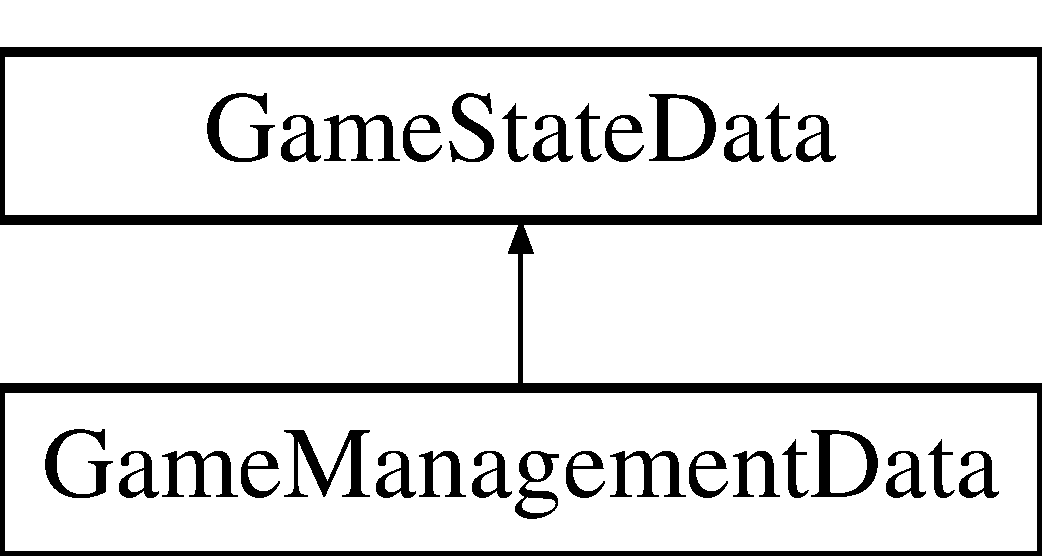
\includegraphics[height=2.000000cm]{classGameStateData}
\end{center}
\end{figure}
\subsection*{Public Member Functions}
\begin{DoxyCompactItemize}
\item 
virtual void \hyperlink{classGameStateData_a28ec2cf2d7dd89bab394b611a83e7d4c}{increase\-P1\-Score} ()=0
\begin{DoxyCompactList}\small\item\em Increment player 1's score by one. \end{DoxyCompactList}\item 
virtual void \hyperlink{classGameStateData_a8b2470bafedd2c51cdc32199ae004b13}{increase\-P2\-Score} ()=0
\begin{DoxyCompactList}\small\item\em Increment player 2's score by one. \end{DoxyCompactList}\item 
virtual const int \hyperlink{classGameStateData_ac4dbf8f19eb4abae6c6e674e1f0ad473}{get\-P1\-Score} ()=0
\begin{DoxyCompactList}\small\item\em Retrieve player 1's score. \end{DoxyCompactList}\item 
virtual const int \hyperlink{classGameStateData_a024affaa547433a0feca091d2bc516b6}{get\-P2\-Score} ()=0
\begin{DoxyCompactList}\small\item\em Retrieve player 2's score. \end{DoxyCompactList}\item 
virtual void \hyperlink{classGameStateData_ab8f2d792862e1292c767d5c1b41eb334}{set\-P1\-Respawn} ()=0
\begin{DoxyCompactList}\small\item\em Allow P1 to be respawed again. \end{DoxyCompactList}\item 
virtual void \hyperlink{classGameStateData_a3b47e49a56e053a7b346b1eafd5c46b1}{set\-P2\-Respawn} ()=0
\begin{DoxyCompactList}\small\item\em Allow P2 to be respawned again. \end{DoxyCompactList}\item 
virtual void \hyperlink{classGameStateData_a0599750aaaa0d272ba8e073d84b0e82b}{disable\-P1\-Respawn} ()=0
\begin{DoxyCompactList}\small\item\em Disallow P1 to be respawned. \end{DoxyCompactList}\item 
virtual void \hyperlink{classGameStateData_a5886e86d10a106cf490eaa2433f3e3ea}{disable\-P2\-Respawn} ()=0
\begin{DoxyCompactList}\small\item\em Disallow P2 to be respawned again. \end{DoxyCompactList}\item 
virtual const bool \hyperlink{classGameStateData_a1893643563270c9ca0552761d0da1085}{is\-P1\-Respawn} ()=0
\begin{DoxyCompactList}\small\item\em Chech to see if P1 can be respawned. \end{DoxyCompactList}\item 
virtual const bool \hyperlink{classGameStateData_af65fd6264b007c67e17ffa23e1b91cdb}{is\-P2\-Respawn} ()=0
\begin{DoxyCompactList}\small\item\em Check to see if P2 can be respawned. \end{DoxyCompactList}\item 
virtual const bool \hyperlink{classGameStateData_a96b7a0057780d2fac25569019804428e}{is\-Game\-Finished} ()=0
\begin{DoxyCompactList}\small\item\em Check to see if the game has reached an end state. \end{DoxyCompactList}\item 
virtual void \hyperlink{classGameStateData_a304d37bb9b7844df62139139bd9cbb92}{set\-Game\-Finished} ()=0
\begin{DoxyCompactList}\small\item\em Set the game to a finnished state. \end{DoxyCompactList}\item 
virtual void \hyperlink{classGameStateData_a1573842cc559d329f894add1678ffb03}{set\-Game\-Time} (const float game\-\_\-time)=0
\begin{DoxyCompactList}\small\item\em Update the game time for rendering. \end{DoxyCompactList}\item 
virtual const float \hyperlink{classGameStateData_a0cb5cf167da9dd1929c719778c5d3506}{get\-Game\-Time} ()=0
\begin{DoxyCompactList}\small\item\em Provide the current game time. \end{DoxyCompactList}\item 
virtual \hyperlink{classGameStateData_a1a607dfe4238a54671e51f1cfab34cd8}{$\sim$\-Game\-State\-Data} ()
\begin{DoxyCompactList}\small\item\em Destructor. \end{DoxyCompactList}\end{DoxyCompactItemize}


\subsection{Detailed Description}


Definition at line 14 of file Game\-State\-Data.\-h.



\subsection{Constructor \& Destructor Documentation}
\hypertarget{classGameStateData_a1a607dfe4238a54671e51f1cfab34cd8}{\index{Game\-State\-Data@{Game\-State\-Data}!$\sim$\-Game\-State\-Data@{$\sim$\-Game\-State\-Data}}
\index{$\sim$\-Game\-State\-Data@{$\sim$\-Game\-State\-Data}!GameStateData@{Game\-State\-Data}}
\subsubsection[{$\sim$\-Game\-State\-Data}]{\setlength{\rightskip}{0pt plus 5cm}virtual Game\-State\-Data\-::$\sim$\-Game\-State\-Data (
\begin{DoxyParamCaption}
{}
\end{DoxyParamCaption}
)\hspace{0.3cm}{\ttfamily [inline]}, {\ttfamily [virtual]}}}\label{classGameStateData_a1a607dfe4238a54671e51f1cfab34cd8}


Destructor. 



Definition at line 46 of file Game\-State\-Data.\-h.


\begin{DoxyCode}
46 \{\};
\end{DoxyCode}


\subsection{Member Function Documentation}
\hypertarget{classGameStateData_a0599750aaaa0d272ba8e073d84b0e82b}{\index{Game\-State\-Data@{Game\-State\-Data}!disable\-P1\-Respawn@{disable\-P1\-Respawn}}
\index{disable\-P1\-Respawn@{disable\-P1\-Respawn}!GameStateData@{Game\-State\-Data}}
\subsubsection[{disable\-P1\-Respawn}]{\setlength{\rightskip}{0pt plus 5cm}virtual void Game\-State\-Data\-::disable\-P1\-Respawn (
\begin{DoxyParamCaption}
{}
\end{DoxyParamCaption}
)\hspace{0.3cm}{\ttfamily [pure virtual]}}}\label{classGameStateData_a0599750aaaa0d272ba8e073d84b0e82b}


Disallow P1 to be respawned. 



Implemented in \hyperlink{classGameManagementData_a66c80fd2795e9e95fe47ad5a77263a9b}{Game\-Management\-Data}.

\hypertarget{classGameStateData_a5886e86d10a106cf490eaa2433f3e3ea}{\index{Game\-State\-Data@{Game\-State\-Data}!disable\-P2\-Respawn@{disable\-P2\-Respawn}}
\index{disable\-P2\-Respawn@{disable\-P2\-Respawn}!GameStateData@{Game\-State\-Data}}
\subsubsection[{disable\-P2\-Respawn}]{\setlength{\rightskip}{0pt plus 5cm}virtual void Game\-State\-Data\-::disable\-P2\-Respawn (
\begin{DoxyParamCaption}
{}
\end{DoxyParamCaption}
)\hspace{0.3cm}{\ttfamily [pure virtual]}}}\label{classGameStateData_a5886e86d10a106cf490eaa2433f3e3ea}


Disallow P2 to be respawned again. 



Implemented in \hyperlink{classGameManagementData_a2bcc4361d645773587a722755f53cf29}{Game\-Management\-Data}.

\hypertarget{classGameStateData_a0cb5cf167da9dd1929c719778c5d3506}{\index{Game\-State\-Data@{Game\-State\-Data}!get\-Game\-Time@{get\-Game\-Time}}
\index{get\-Game\-Time@{get\-Game\-Time}!GameStateData@{Game\-State\-Data}}
\subsubsection[{get\-Game\-Time}]{\setlength{\rightskip}{0pt plus 5cm}virtual const float Game\-State\-Data\-::get\-Game\-Time (
\begin{DoxyParamCaption}
{}
\end{DoxyParamCaption}
)\hspace{0.3cm}{\ttfamily [pure virtual]}}}\label{classGameStateData_a0cb5cf167da9dd1929c719778c5d3506}


Provide the current game time. 



Implemented in \hyperlink{classGameManagementData_aa507f9e395464888ad9dc66a90b1bbc3}{Game\-Management\-Data}.



Referenced by Draw\-Manager\-::manage().

\hypertarget{classGameStateData_ac4dbf8f19eb4abae6c6e674e1f0ad473}{\index{Game\-State\-Data@{Game\-State\-Data}!get\-P1\-Score@{get\-P1\-Score}}
\index{get\-P1\-Score@{get\-P1\-Score}!GameStateData@{Game\-State\-Data}}
\subsubsection[{get\-P1\-Score}]{\setlength{\rightskip}{0pt plus 5cm}virtual const int Game\-State\-Data\-::get\-P1\-Score (
\begin{DoxyParamCaption}
{}
\end{DoxyParamCaption}
)\hspace{0.3cm}{\ttfamily [pure virtual]}}}\label{classGameStateData_ac4dbf8f19eb4abae6c6e674e1f0ad473}


Retrieve player 1's score. 



Implemented in \hyperlink{classGameManagementData_a2738ec4d85bdb87f957d21e8a314e502}{Game\-Management\-Data}.



Referenced by Draw\-Manager\-::manage().

\hypertarget{classGameStateData_a024affaa547433a0feca091d2bc516b6}{\index{Game\-State\-Data@{Game\-State\-Data}!get\-P2\-Score@{get\-P2\-Score}}
\index{get\-P2\-Score@{get\-P2\-Score}!GameStateData@{Game\-State\-Data}}
\subsubsection[{get\-P2\-Score}]{\setlength{\rightskip}{0pt plus 5cm}virtual const int Game\-State\-Data\-::get\-P2\-Score (
\begin{DoxyParamCaption}
{}
\end{DoxyParamCaption}
)\hspace{0.3cm}{\ttfamily [pure virtual]}}}\label{classGameStateData_a024affaa547433a0feca091d2bc516b6}


Retrieve player 2's score. 



Implemented in \hyperlink{classGameManagementData_ad1d991be2ab8b8f814ef6898dd887d15}{Game\-Management\-Data}.



Referenced by Draw\-Manager\-::manage().

\hypertarget{classGameStateData_a28ec2cf2d7dd89bab394b611a83e7d4c}{\index{Game\-State\-Data@{Game\-State\-Data}!increase\-P1\-Score@{increase\-P1\-Score}}
\index{increase\-P1\-Score@{increase\-P1\-Score}!GameStateData@{Game\-State\-Data}}
\subsubsection[{increase\-P1\-Score}]{\setlength{\rightskip}{0pt plus 5cm}virtual void Game\-State\-Data\-::increase\-P1\-Score (
\begin{DoxyParamCaption}
{}
\end{DoxyParamCaption}
)\hspace{0.3cm}{\ttfamily [pure virtual]}}}\label{classGameStateData_a28ec2cf2d7dd89bab394b611a83e7d4c}


Increment player 1's score by one. 



Implemented in \hyperlink{classGameManagementData_a7d574170fe76a837c05372c8c52eed63}{Game\-Management\-Data}.



Referenced by Destruction\-Manager\-::manage().

\hypertarget{classGameStateData_a8b2470bafedd2c51cdc32199ae004b13}{\index{Game\-State\-Data@{Game\-State\-Data}!increase\-P2\-Score@{increase\-P2\-Score}}
\index{increase\-P2\-Score@{increase\-P2\-Score}!GameStateData@{Game\-State\-Data}}
\subsubsection[{increase\-P2\-Score}]{\setlength{\rightskip}{0pt plus 5cm}virtual void Game\-State\-Data\-::increase\-P2\-Score (
\begin{DoxyParamCaption}
{}
\end{DoxyParamCaption}
)\hspace{0.3cm}{\ttfamily [pure virtual]}}}\label{classGameStateData_a8b2470bafedd2c51cdc32199ae004b13}


Increment player 2's score by one. 



Implemented in \hyperlink{classGameManagementData_a9a7a124ef719be6f9d45c4ec231e7774}{Game\-Management\-Data}.



Referenced by Destruction\-Manager\-::manage().

\hypertarget{classGameStateData_a96b7a0057780d2fac25569019804428e}{\index{Game\-State\-Data@{Game\-State\-Data}!is\-Game\-Finished@{is\-Game\-Finished}}
\index{is\-Game\-Finished@{is\-Game\-Finished}!GameStateData@{Game\-State\-Data}}
\subsubsection[{is\-Game\-Finished}]{\setlength{\rightskip}{0pt plus 5cm}virtual const bool Game\-State\-Data\-::is\-Game\-Finished (
\begin{DoxyParamCaption}
{}
\end{DoxyParamCaption}
)\hspace{0.3cm}{\ttfamily [pure virtual]}}}\label{classGameStateData_a96b7a0057780d2fac25569019804428e}


Check to see if the game has reached an end state. 



Implemented in \hyperlink{classGameManagementData_ac8d6deb9285fe8e5205f9984b0a2622d}{Game\-Management\-Data}.

\hypertarget{classGameStateData_a1893643563270c9ca0552761d0da1085}{\index{Game\-State\-Data@{Game\-State\-Data}!is\-P1\-Respawn@{is\-P1\-Respawn}}
\index{is\-P1\-Respawn@{is\-P1\-Respawn}!GameStateData@{Game\-State\-Data}}
\subsubsection[{is\-P1\-Respawn}]{\setlength{\rightskip}{0pt plus 5cm}virtual const bool Game\-State\-Data\-::is\-P1\-Respawn (
\begin{DoxyParamCaption}
{}
\end{DoxyParamCaption}
)\hspace{0.3cm}{\ttfamily [pure virtual]}}}\label{classGameStateData_a1893643563270c9ca0552761d0da1085}


Chech to see if P1 can be respawned. 



Implemented in \hyperlink{classGameManagementData_a2abb452bd5ecd1f8d09b76dc1f909260}{Game\-Management\-Data}.

\hypertarget{classGameStateData_af65fd6264b007c67e17ffa23e1b91cdb}{\index{Game\-State\-Data@{Game\-State\-Data}!is\-P2\-Respawn@{is\-P2\-Respawn}}
\index{is\-P2\-Respawn@{is\-P2\-Respawn}!GameStateData@{Game\-State\-Data}}
\subsubsection[{is\-P2\-Respawn}]{\setlength{\rightskip}{0pt plus 5cm}virtual const bool Game\-State\-Data\-::is\-P2\-Respawn (
\begin{DoxyParamCaption}
{}
\end{DoxyParamCaption}
)\hspace{0.3cm}{\ttfamily [pure virtual]}}}\label{classGameStateData_af65fd6264b007c67e17ffa23e1b91cdb}


Check to see if P2 can be respawned. 



Implemented in \hyperlink{classGameManagementData_a3b94efaf212d65515c1c511a17636b5f}{Game\-Management\-Data}.

\hypertarget{classGameStateData_a304d37bb9b7844df62139139bd9cbb92}{\index{Game\-State\-Data@{Game\-State\-Data}!set\-Game\-Finished@{set\-Game\-Finished}}
\index{set\-Game\-Finished@{set\-Game\-Finished}!GameStateData@{Game\-State\-Data}}
\subsubsection[{set\-Game\-Finished}]{\setlength{\rightskip}{0pt plus 5cm}virtual void Game\-State\-Data\-::set\-Game\-Finished (
\begin{DoxyParamCaption}
{}
\end{DoxyParamCaption}
)\hspace{0.3cm}{\ttfamily [pure virtual]}}}\label{classGameStateData_a304d37bb9b7844df62139139bd9cbb92}


Set the game to a finnished state. 



Implemented in \hyperlink{classGameManagementData_afef95ac9618619ca6ec29277fd04c361}{Game\-Management\-Data}.

\hypertarget{classGameStateData_a1573842cc559d329f894add1678ffb03}{\index{Game\-State\-Data@{Game\-State\-Data}!set\-Game\-Time@{set\-Game\-Time}}
\index{set\-Game\-Time@{set\-Game\-Time}!GameStateData@{Game\-State\-Data}}
\subsubsection[{set\-Game\-Time}]{\setlength{\rightskip}{0pt plus 5cm}virtual void Game\-State\-Data\-::set\-Game\-Time (
\begin{DoxyParamCaption}
\item[{const float}]{game\-\_\-time}
\end{DoxyParamCaption}
)\hspace{0.3cm}{\ttfamily [pure virtual]}}}\label{classGameStateData_a1573842cc559d329f894add1678ffb03}


Update the game time for rendering. 



Implemented in \hyperlink{classGameManagementData_ae3ed7d9a9cbed2222ad34c52a4bcfd5c}{Game\-Management\-Data}.

\hypertarget{classGameStateData_ab8f2d792862e1292c767d5c1b41eb334}{\index{Game\-State\-Data@{Game\-State\-Data}!set\-P1\-Respawn@{set\-P1\-Respawn}}
\index{set\-P1\-Respawn@{set\-P1\-Respawn}!GameStateData@{Game\-State\-Data}}
\subsubsection[{set\-P1\-Respawn}]{\setlength{\rightskip}{0pt plus 5cm}virtual void Game\-State\-Data\-::set\-P1\-Respawn (
\begin{DoxyParamCaption}
{}
\end{DoxyParamCaption}
)\hspace{0.3cm}{\ttfamily [pure virtual]}}}\label{classGameStateData_ab8f2d792862e1292c767d5c1b41eb334}


Allow P1 to be respawed again. 



Implemented in \hyperlink{classGameManagementData_a1df14e6642056790f6677cbd779c6815}{Game\-Management\-Data}.

\hypertarget{classGameStateData_a3b47e49a56e053a7b346b1eafd5c46b1}{\index{Game\-State\-Data@{Game\-State\-Data}!set\-P2\-Respawn@{set\-P2\-Respawn}}
\index{set\-P2\-Respawn@{set\-P2\-Respawn}!GameStateData@{Game\-State\-Data}}
\subsubsection[{set\-P2\-Respawn}]{\setlength{\rightskip}{0pt plus 5cm}virtual void Game\-State\-Data\-::set\-P2\-Respawn (
\begin{DoxyParamCaption}
{}
\end{DoxyParamCaption}
)\hspace{0.3cm}{\ttfamily [pure virtual]}}}\label{classGameStateData_a3b47e49a56e053a7b346b1eafd5c46b1}


Allow P2 to be respawned again. 



Implemented in \hyperlink{classGameManagementData_a31113c80e1caa2604c98db63d565641a}{Game\-Management\-Data}.



The documentation for this class was generated from the following file\-:\begin{DoxyCompactItemize}
\item 
\hyperlink{GameStateData_8h}{Game\-State\-Data.\-h}\end{DoxyCompactItemize}

\hypertarget{classGameStateManager}{\section{Game\-State\-Manager Class Reference}
\label{classGameStateManager}\index{Game\-State\-Manager@{Game\-State\-Manager}}
}


\hyperlink{classManager}{Manager} class responsible for managing state of the game.  




{\ttfamily \#include $<$Game\-State\-Manager.\-h$>$}

Inheritance diagram for Game\-State\-Manager\-:\begin{figure}[H]
\begin{center}
\leavevmode
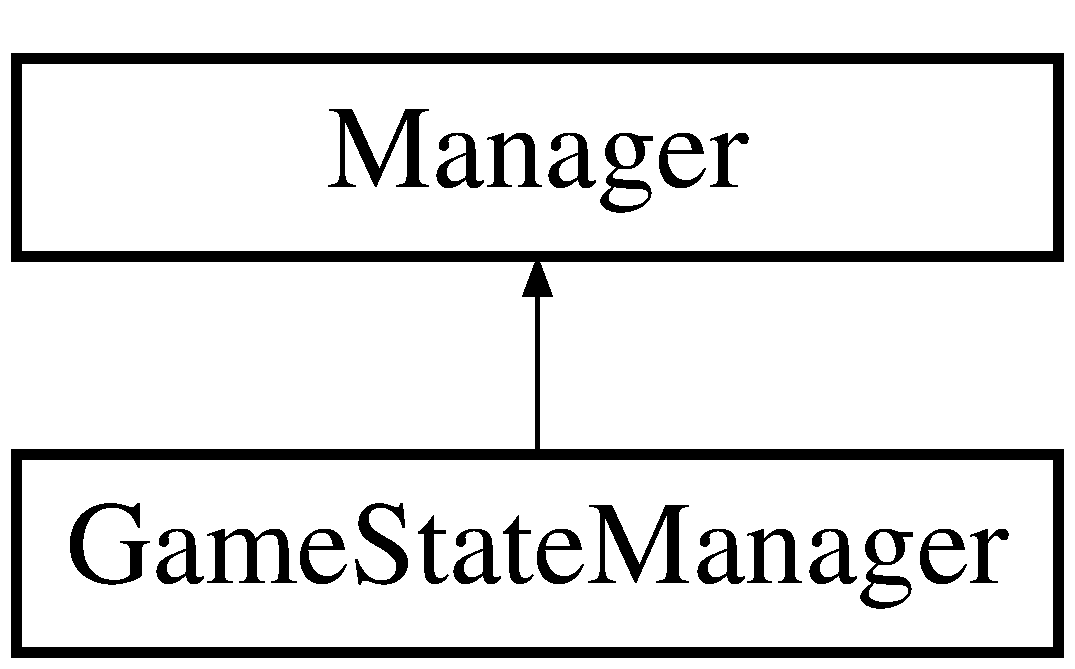
\includegraphics[height=2.000000cm]{classGameStateManager}
\end{center}
\end{figure}
\subsection*{Public Member Functions}
\begin{DoxyCompactItemize}
\item 
\hyperlink{classGameStateManager_aa9769dca27ad070cf5491a7f54c7d85e}{Game\-State\-Manager} ()
\begin{DoxyCompactList}\small\item\em Constructor for \hyperlink{classGameStateManager}{Game\-State\-Manager}. \end{DoxyCompactList}\item 
void \hyperlink{classGameStateManager_aa113f5c0f62142776ec8cef1bb904ff5}{manage} (\hyperlink{classGameManagementData}{Game\-Management\-Data} \&game\-\_\-data\-\_\-container)
\begin{DoxyCompactList}\small\item\em Main manage function. \end{DoxyCompactList}\item 
\hyperlink{classGameStateManager_ad20961eb5d9ed6b7ef764037d5e11ba5}{$\sim$\-Game\-State\-Manager} ()
\end{DoxyCompactItemize}
\subsection*{Private Member Functions}
\begin{DoxyCompactItemize}
\item 
void \hyperlink{classGameStateManager_a5b61abb4ee2058208277bc7e6e19eda9}{manage\-Attack\-Timers} (\hyperlink{classActionData}{Action\-Data} \&action\-\_\-data\-\_\-container)
\begin{DoxyCompactList}\small\item\em Manage the timers that keep track of firing and laying mines intervals. \end{DoxyCompactList}\item 
bool \hyperlink{classGameStateManager_af8588ab062f78314e0d22faefae3c834}{time\-Run\-Out} (\hyperlink{classStopWatch}{Stop\-Watch} \&timer)
\begin{DoxyCompactList}\small\item\em Checks timeout for specific timer. \end{DoxyCompactList}\end{DoxyCompactItemize}
\subsection*{Private Attributes}
\begin{DoxyCompactItemize}
\item 
\hyperlink{classStopWatch}{Stop\-Watch} \hyperlink{classGameStateManager_a059c0be895a3ed3632257fbeb65b86d9}{\-\_\-game\-\_\-timer}
\begin{DoxyCompactList}\small\item\em Keeps track of the overall game time. \end{DoxyCompactList}\item 
\hyperlink{classStopWatch}{Stop\-Watch} \hyperlink{classGameStateManager_a56b5da52f57018c53a29ee4adef4acff}{\-\_\-p1\-\_\-fire\-\_\-timer}
\begin{DoxyCompactList}\small\item\em Keep tracks of time between firing of missiles for player 1. \end{DoxyCompactList}\item 
\hyperlink{classStopWatch}{Stop\-Watch} \hyperlink{classGameStateManager_a6ffa94597eef770ae4c812a834daa39c}{\-\_\-p2\-\_\-fire\-\_\-timer}
\begin{DoxyCompactList}\small\item\em Keep tracks of time between firing of missiles for player 2. \end{DoxyCompactList}\item 
\hyperlink{classStopWatch}{Stop\-Watch} \hyperlink{classGameStateManager_a7e424def0f4a2f1548b5b63629cd66f1}{\-\_\-p1\-\_\-lay\-\_\-mine\-\_\-timer}
\begin{DoxyCompactList}\small\item\em Keeps track of time between laying mines for player 1. \end{DoxyCompactList}\item 
\hyperlink{classStopWatch}{Stop\-Watch} \hyperlink{classGameStateManager_a14203d39640e3368bc75c2e9b853a452}{\-\_\-p2\-\_\-lay\-\_\-mine\-\_\-timer}
\begin{DoxyCompactList}\small\item\em Keeps track of time between laying mines for player 2. \end{DoxyCompactList}\item 
const double \hyperlink{classGameStateManager_a225d7168ceade083143153748bd55264}{\-\_\-game\-\_\-runtime} = 120.\-0
\begin{DoxyCompactList}\small\item\em The time in seconds of how long the game will last. \end{DoxyCompactList}\item 
const double \hyperlink{classGameStateManager_a94f553200fdb06e224376f60c0bcec4f}{\-\_\-attack\-\_\-time\-\_\-limit} = 0.\-5
\begin{DoxyCompactList}\small\item\em Time limit between firing or laying mines for tanks. \end{DoxyCompactList}\end{DoxyCompactItemize}


\subsection{Detailed Description}
\hyperlink{classManager}{Manager} class responsible for managing state of the game. 

Definition at line 23 of file Game\-State\-Manager.\-h.



\subsection{Constructor \& Destructor Documentation}
\hypertarget{classGameStateManager_aa9769dca27ad070cf5491a7f54c7d85e}{\index{Game\-State\-Manager@{Game\-State\-Manager}!Game\-State\-Manager@{Game\-State\-Manager}}
\index{Game\-State\-Manager@{Game\-State\-Manager}!GameStateManager@{Game\-State\-Manager}}
\subsubsection[{Game\-State\-Manager}]{\setlength{\rightskip}{0pt plus 5cm}Game\-State\-Manager\-::\-Game\-State\-Manager (
\begin{DoxyParamCaption}
{}
\end{DoxyParamCaption}
)}}\label{classGameStateManager_aa9769dca27ad070cf5491a7f54c7d85e}


Constructor for \hyperlink{classGameStateManager}{Game\-State\-Manager}. 

Initialises the timer for the whole game. 

Definition at line 17 of file Game\-State\-Manager.\-cpp.



References \-\_\-game\-\_\-timer, and Stop\-Watch\-::start().


\begin{DoxyCode}
18 \{
19     \hyperlink{classGameStateManager_a059c0be895a3ed3632257fbeb65b86d9}{\_game\_timer}.\hyperlink{classStopWatch_a09a3c8f9ab03d7b28e4f8b90a833974e}{start}();
20 \}
\end{DoxyCode}
\hypertarget{classGameStateManager_ad20961eb5d9ed6b7ef764037d5e11ba5}{\index{Game\-State\-Manager@{Game\-State\-Manager}!$\sim$\-Game\-State\-Manager@{$\sim$\-Game\-State\-Manager}}
\index{$\sim$\-Game\-State\-Manager@{$\sim$\-Game\-State\-Manager}!GameStateManager@{Game\-State\-Manager}}
\subsubsection[{$\sim$\-Game\-State\-Manager}]{\setlength{\rightskip}{0pt plus 5cm}Game\-State\-Manager\-::$\sim$\-Game\-State\-Manager (
\begin{DoxyParamCaption}
{}
\end{DoxyParamCaption}
)}}\label{classGameStateManager_ad20961eb5d9ed6b7ef764037d5e11ba5}


Definition at line 105 of file Game\-State\-Manager.\-cpp.


\begin{DoxyCode}
106 \{
107 
108 \}
\end{DoxyCode}


\subsection{Member Function Documentation}
\hypertarget{classGameStateManager_aa113f5c0f62142776ec8cef1bb904ff5}{\index{Game\-State\-Manager@{Game\-State\-Manager}!manage@{manage}}
\index{manage@{manage}!GameStateManager@{Game\-State\-Manager}}
\subsubsection[{manage}]{\setlength{\rightskip}{0pt plus 5cm}void Game\-State\-Manager\-::manage (
\begin{DoxyParamCaption}
\item[{{\bf Game\-Management\-Data} \&}]{game\-\_\-data\-\_\-container}
\end{DoxyParamCaption}
)}}\label{classGameStateManager_aa113f5c0f62142776ec8cef1bb904ff5}


Main manage function. 

The amount of elapsed time is obtained by getting the timer value and subtracting that from the game runtime variable. Once that timer runs out, the game state will be set to finished. Otherwise the current game time is set. Attack timers are also run. 
\begin{DoxyParams}{Parameters}
{\em game\-\_\-data\-\_\-container} & \-:\-: Information that holds the game time which will be changed accordingly \\
\hline
\end{DoxyParams}


Definition at line 28 of file Game\-State\-Manager.\-cpp.



References \-\_\-game\-\_\-runtime, \-\_\-game\-\_\-timer, Stop\-Watch\-::get\-Timer\-Value(), Stop\-Watch\-::is\-Running(), manage\-Attack\-Timers(), Game\-Management\-Data\-::set\-Game\-Finished(), Game\-Management\-Data\-::set\-Game\-Time(), Stop\-Watch\-::start(), and Stop\-Watch\-::stop().



Referenced by Game\-::run\-All\-Managers(), and T\-E\-S\-T().


\begin{DoxyCode}
29 \{
30     \textcolor{keywordflow}{if} (!\hyperlink{classGameStateManager_a059c0be895a3ed3632257fbeb65b86d9}{\_game\_timer}.\hyperlink{classStopWatch_a4358045d32002cb83ec62d1ebb9fb5ca}{isRunning}())
31         \hyperlink{classGameStateManager_a059c0be895a3ed3632257fbeb65b86d9}{\_game\_timer}.\hyperlink{classStopWatch_a09a3c8f9ab03d7b28e4f8b90a833974e}{start}();
32 
33     \textcolor{keywordtype}{double} current\_time = \hyperlink{classGameStateManager_a225d7168ceade083143153748bd55264}{\_game\_runtime} - \hyperlink{classGameStateManager_a059c0be895a3ed3632257fbeb65b86d9}{\_game\_timer}.
      \hyperlink{classStopWatch_a29945e425c084bb7df859c4c10cbd9fe}{getTimerValue}();\textcolor{comment}{// makes the timer countdown}
34 
35     \textcolor{keywordflow}{if} (current\_time <= 0 )
36     \{
37         \hyperlink{classGameStateManager_a059c0be895a3ed3632257fbeb65b86d9}{\_game\_timer}.\hyperlink{classStopWatch_a6e80b598d9304e37d8768b716e713e0e}{stop}();
38         game\_data\_container.\hyperlink{classGameManagementData_afef95ac9618619ca6ec29277fd04c361}{setGameFinished}(); \textcolor{comment}{// finish the game}
39     \}
40     \textcolor{keywordflow}{else}
41         game\_data\_container.\hyperlink{classGameManagementData_ae3ed7d9a9cbed2222ad34c52a4bcfd5c}{setGameTime}(current\_time);
42 
43     \hyperlink{classGameStateManager_a5b61abb4ee2058208277bc7e6e19eda9}{manageAttackTimers}(game\_data\_container);
44 \}
\end{DoxyCode}
\hypertarget{classGameStateManager_a5b61abb4ee2058208277bc7e6e19eda9}{\index{Game\-State\-Manager@{Game\-State\-Manager}!manage\-Attack\-Timers@{manage\-Attack\-Timers}}
\index{manage\-Attack\-Timers@{manage\-Attack\-Timers}!GameStateManager@{Game\-State\-Manager}}
\subsubsection[{manage\-Attack\-Timers}]{\setlength{\rightskip}{0pt plus 5cm}void Game\-State\-Manager\-::manage\-Attack\-Timers (
\begin{DoxyParamCaption}
\item[{{\bf Action\-Data} \&}]{game\-\_\-data\-\_\-container}
\end{DoxyParamCaption}
)\hspace{0.3cm}{\ttfamily [private]}}}\label{classGameStateManager_a5b61abb4ee2058208277bc7e6e19eda9}


Manage the timers that keep track of firing and laying mines intervals. 

Both players' timers are checked. If their time for firing has run out then thay may fire another missile, or lay another mine. 
\begin{DoxyParams}{Parameters}
{\em game\-\_\-data\-\_\-container} & \-:\-: Information about whhat attacks the players' desire \\
\hline
\end{DoxyParams}


Definition at line 51 of file Game\-State\-Manager.\-cpp.



References \-\_\-p1\-\_\-fire\-\_\-timer, \-\_\-p1\-\_\-lay\-\_\-mine\-\_\-timer, \-\_\-p2\-\_\-fire\-\_\-timer, \-\_\-p2\-\_\-lay\-\_\-mine\-\_\-timer, fire\-\_\-missile, Action\-Data\-::give\-Action\-Info(), lay\-\_\-mine, Action\-Data\-::reset\-P1\-Attack(), Action\-Data\-::reset\-P2\-Attack(), and time\-Run\-Out().



Referenced by manage().


\begin{DoxyCode}
52 \{
53     \textcolor{keyword}{auto} actions = game\_data\_container.\hyperlink{classActionData_ab2f5b210968c91a01ed1439904b3ffee}{giveActionInfo}();
54 
55     \textcolor{keywordflow}{if} (actions.attack\_1 == \hyperlink{Structures_8h_abf3d9daa4559fb2f9e16fc1836fead1badfc8afb4acc9eae75dcfdde515861288}{fire\_missile})
56     \{
57         \textcolor{keywordflow}{if} (!\hyperlink{classGameStateManager_af8588ab062f78314e0d22faefae3c834}{timeRunOut}(\hyperlink{classGameStateManager_a56b5da52f57018c53a29ee4adef4acff}{\_p1\_fire\_timer}))
58             game\_data\_container.\hyperlink{classActionData_a12925d051a1cd40bddcb18f0be2c2b01}{resetP1Attack}();
59     \}
60 
61     \textcolor{keywordflow}{if} (actions.attack\_2 == \hyperlink{Structures_8h_abf3d9daa4559fb2f9e16fc1836fead1badfc8afb4acc9eae75dcfdde515861288}{fire\_missile})
62     \{
63         \textcolor{keywordflow}{if} (!\hyperlink{classGameStateManager_af8588ab062f78314e0d22faefae3c834}{timeRunOut}(\hyperlink{classGameStateManager_a6ffa94597eef770ae4c812a834daa39c}{\_p2\_fire\_timer}))
64             game\_data\_container.\hyperlink{classActionData_ab8a96447019bfc7a275903dfa42cfcf5}{resetP2Attack}();
65     \}
66 
67 
68     \textcolor{keywordflow}{if} (actions.attack\_1 == \hyperlink{Structures_8h_abf3d9daa4559fb2f9e16fc1836fead1baed59f3b92945ae37d3f2f4e7472acacc}{lay\_mine})
69     \{
70         \textcolor{keywordflow}{if} (!\hyperlink{classGameStateManager_af8588ab062f78314e0d22faefae3c834}{timeRunOut}(\hyperlink{classGameStateManager_a7e424def0f4a2f1548b5b63629cd66f1}{\_p1\_lay\_mine\_timer}))
71             game\_data\_container.\hyperlink{classActionData_a12925d051a1cd40bddcb18f0be2c2b01}{resetP1Attack}();
72     \}
73 
74     \textcolor{keywordflow}{if} (actions.attack\_2 == \hyperlink{Structures_8h_abf3d9daa4559fb2f9e16fc1836fead1baed59f3b92945ae37d3f2f4e7472acacc}{lay\_mine})
75     \{
76         \textcolor{keywordflow}{if} (!\hyperlink{classGameStateManager_af8588ab062f78314e0d22faefae3c834}{timeRunOut}(\hyperlink{classGameStateManager_a14203d39640e3368bc75c2e9b853a452}{\_p2\_lay\_mine\_timer}))
77             game\_data\_container.\hyperlink{classActionData_ab8a96447019bfc7a275903dfa42cfcf5}{resetP2Attack}();
78     \}
79 \}
\end{DoxyCode}
\hypertarget{classGameStateManager_af8588ab062f78314e0d22faefae3c834}{\index{Game\-State\-Manager@{Game\-State\-Manager}!time\-Run\-Out@{time\-Run\-Out}}
\index{time\-Run\-Out@{time\-Run\-Out}!GameStateManager@{Game\-State\-Manager}}
\subsubsection[{time\-Run\-Out}]{\setlength{\rightskip}{0pt plus 5cm}bool Game\-State\-Manager\-::time\-Run\-Out (
\begin{DoxyParamCaption}
\item[{{\bf Stop\-Watch} \&}]{timer}
\end{DoxyParamCaption}
)\hspace{0.3cm}{\ttfamily [private]}}}\label{classGameStateManager_af8588ab062f78314e0d22faefae3c834}


Checks timeout for specific timer. 

If the timer is not running yet, then it is started. If it has started, the attack time is calculated. 
\begin{DoxyParams}{Parameters}
{\em timer} & \-:\-: timer to be checked \\
\hline
\end{DoxyParams}
\begin{DoxyReturn}{Returns}
bool 
\end{DoxyReturn}


Definition at line 87 of file Game\-State\-Manager.\-cpp.



References \-\_\-attack\-\_\-time\-\_\-limit, Stop\-Watch\-::get\-Timer\-Value(), Stop\-Watch\-::is\-Running(), Stop\-Watch\-::reset(), and Stop\-Watch\-::start().



Referenced by manage\-Attack\-Timers().


\begin{DoxyCode}
88 \{
89     \textcolor{keywordflow}{if} (!timer.\hyperlink{classStopWatch_a4358045d32002cb83ec62d1ebb9fb5ca}{isRunning}())
90     \{
91         timer.\hyperlink{classStopWatch_a09a3c8f9ab03d7b28e4f8b90a833974e}{start}();
92         \textcolor{keywordflow}{return} \textcolor{keyword}{true};
93     \}
94 
95     \textcolor{keywordtype}{double} timer\_time = \hyperlink{classGameStateManager_a94f553200fdb06e224376f60c0bcec4f}{\_attack\_time\_limit} - timer.
      \hyperlink{classStopWatch_a29945e425c084bb7df859c4c10cbd9fe}{getTimerValue}();
96     \textcolor{keywordflow}{if} (timer\_time <= 0)
97     \{
98         timer.\hyperlink{classStopWatch_a1c0dcc57c615559f24bc9f8759271a9d}{reset}();
99         \textcolor{keywordflow}{return} \textcolor{keyword}{true};
100     \}
101     \textcolor{keywordflow}{else} \textcolor{keywordflow}{return} \textcolor{keyword}{false};
102 
103 \}
\end{DoxyCode}


\subsection{Member Data Documentation}
\hypertarget{classGameStateManager_a94f553200fdb06e224376f60c0bcec4f}{\index{Game\-State\-Manager@{Game\-State\-Manager}!\-\_\-attack\-\_\-time\-\_\-limit@{\-\_\-attack\-\_\-time\-\_\-limit}}
\index{\-\_\-attack\-\_\-time\-\_\-limit@{\-\_\-attack\-\_\-time\-\_\-limit}!GameStateManager@{Game\-State\-Manager}}
\subsubsection[{\-\_\-attack\-\_\-time\-\_\-limit}]{\setlength{\rightskip}{0pt plus 5cm}const double Game\-State\-Manager\-::\-\_\-attack\-\_\-time\-\_\-limit = 0.\-5\hspace{0.3cm}{\ttfamily [private]}}}\label{classGameStateManager_a94f553200fdb06e224376f60c0bcec4f}


Time limit between firing or laying mines for tanks. 



Definition at line 44 of file Game\-State\-Manager.\-h.



Referenced by time\-Run\-Out().

\hypertarget{classGameStateManager_a225d7168ceade083143153748bd55264}{\index{Game\-State\-Manager@{Game\-State\-Manager}!\-\_\-game\-\_\-runtime@{\-\_\-game\-\_\-runtime}}
\index{\-\_\-game\-\_\-runtime@{\-\_\-game\-\_\-runtime}!GameStateManager@{Game\-State\-Manager}}
\subsubsection[{\-\_\-game\-\_\-runtime}]{\setlength{\rightskip}{0pt plus 5cm}const double Game\-State\-Manager\-::\-\_\-game\-\_\-runtime = 120.\-0\hspace{0.3cm}{\ttfamily [private]}}}\label{classGameStateManager_a225d7168ceade083143153748bd55264}


The time in seconds of how long the game will last. 



Definition at line 42 of file Game\-State\-Manager.\-h.



Referenced by manage().

\hypertarget{classGameStateManager_a059c0be895a3ed3632257fbeb65b86d9}{\index{Game\-State\-Manager@{Game\-State\-Manager}!\-\_\-game\-\_\-timer@{\-\_\-game\-\_\-timer}}
\index{\-\_\-game\-\_\-timer@{\-\_\-game\-\_\-timer}!GameStateManager@{Game\-State\-Manager}}
\subsubsection[{\-\_\-game\-\_\-timer}]{\setlength{\rightskip}{0pt plus 5cm}{\bf Stop\-Watch} Game\-State\-Manager\-::\-\_\-game\-\_\-timer\hspace{0.3cm}{\ttfamily [private]}}}\label{classGameStateManager_a059c0be895a3ed3632257fbeb65b86d9}


Keeps track of the overall game time. 



Definition at line 32 of file Game\-State\-Manager.\-h.



Referenced by Game\-State\-Manager(), and manage().

\hypertarget{classGameStateManager_a56b5da52f57018c53a29ee4adef4acff}{\index{Game\-State\-Manager@{Game\-State\-Manager}!\-\_\-p1\-\_\-fire\-\_\-timer@{\-\_\-p1\-\_\-fire\-\_\-timer}}
\index{\-\_\-p1\-\_\-fire\-\_\-timer@{\-\_\-p1\-\_\-fire\-\_\-timer}!GameStateManager@{Game\-State\-Manager}}
\subsubsection[{\-\_\-p1\-\_\-fire\-\_\-timer}]{\setlength{\rightskip}{0pt plus 5cm}{\bf Stop\-Watch} Game\-State\-Manager\-::\-\_\-p1\-\_\-fire\-\_\-timer\hspace{0.3cm}{\ttfamily [private]}}}\label{classGameStateManager_a56b5da52f57018c53a29ee4adef4acff}


Keep tracks of time between firing of missiles for player 1. 



Definition at line 34 of file Game\-State\-Manager.\-h.



Referenced by manage\-Attack\-Timers().

\hypertarget{classGameStateManager_a7e424def0f4a2f1548b5b63629cd66f1}{\index{Game\-State\-Manager@{Game\-State\-Manager}!\-\_\-p1\-\_\-lay\-\_\-mine\-\_\-timer@{\-\_\-p1\-\_\-lay\-\_\-mine\-\_\-timer}}
\index{\-\_\-p1\-\_\-lay\-\_\-mine\-\_\-timer@{\-\_\-p1\-\_\-lay\-\_\-mine\-\_\-timer}!GameStateManager@{Game\-State\-Manager}}
\subsubsection[{\-\_\-p1\-\_\-lay\-\_\-mine\-\_\-timer}]{\setlength{\rightskip}{0pt plus 5cm}{\bf Stop\-Watch} Game\-State\-Manager\-::\-\_\-p1\-\_\-lay\-\_\-mine\-\_\-timer\hspace{0.3cm}{\ttfamily [private]}}}\label{classGameStateManager_a7e424def0f4a2f1548b5b63629cd66f1}


Keeps track of time between laying mines for player 1. 



Definition at line 38 of file Game\-State\-Manager.\-h.



Referenced by manage\-Attack\-Timers().

\hypertarget{classGameStateManager_a6ffa94597eef770ae4c812a834daa39c}{\index{Game\-State\-Manager@{Game\-State\-Manager}!\-\_\-p2\-\_\-fire\-\_\-timer@{\-\_\-p2\-\_\-fire\-\_\-timer}}
\index{\-\_\-p2\-\_\-fire\-\_\-timer@{\-\_\-p2\-\_\-fire\-\_\-timer}!GameStateManager@{Game\-State\-Manager}}
\subsubsection[{\-\_\-p2\-\_\-fire\-\_\-timer}]{\setlength{\rightskip}{0pt plus 5cm}{\bf Stop\-Watch} Game\-State\-Manager\-::\-\_\-p2\-\_\-fire\-\_\-timer\hspace{0.3cm}{\ttfamily [private]}}}\label{classGameStateManager_a6ffa94597eef770ae4c812a834daa39c}


Keep tracks of time between firing of missiles for player 2. 



Definition at line 36 of file Game\-State\-Manager.\-h.



Referenced by manage\-Attack\-Timers().

\hypertarget{classGameStateManager_a14203d39640e3368bc75c2e9b853a452}{\index{Game\-State\-Manager@{Game\-State\-Manager}!\-\_\-p2\-\_\-lay\-\_\-mine\-\_\-timer@{\-\_\-p2\-\_\-lay\-\_\-mine\-\_\-timer}}
\index{\-\_\-p2\-\_\-lay\-\_\-mine\-\_\-timer@{\-\_\-p2\-\_\-lay\-\_\-mine\-\_\-timer}!GameStateManager@{Game\-State\-Manager}}
\subsubsection[{\-\_\-p2\-\_\-lay\-\_\-mine\-\_\-timer}]{\setlength{\rightskip}{0pt plus 5cm}{\bf Stop\-Watch} Game\-State\-Manager\-::\-\_\-p2\-\_\-lay\-\_\-mine\-\_\-timer\hspace{0.3cm}{\ttfamily [private]}}}\label{classGameStateManager_a14203d39640e3368bc75c2e9b853a452}


Keeps track of time between laying mines for player 2. 



Definition at line 40 of file Game\-State\-Manager.\-h.



Referenced by manage\-Attack\-Timers().



The documentation for this class was generated from the following files\-:\begin{DoxyCompactItemize}
\item 
\hyperlink{GameStateManager_8h}{Game\-State\-Manager.\-h}\item 
\hyperlink{GameStateManager_8cpp}{Game\-State\-Manager.\-cpp}\end{DoxyCompactItemize}

\hypertarget{classGeometryEngine}{\section{Geometry\-Engine Class Reference}
\label{classGeometryEngine}\index{Geometry\-Engine@{Geometry\-Engine}}
}


Class responisible for handling geometrical calculations.  




{\ttfamily \#include $<$Geometry\-Engine.\-h$>$}

\subsection*{Public Member Functions}
\begin{DoxyCompactItemize}
\item 
bool \hyperlink{classGeometryEngine_a049acffe89f53be25fbc9d4018c3b388}{is\-Collision} (const \hyperlink{structrect__corners}{rect\-\_\-corners} \&rect\-\_\-\-A, const \hyperlink{structrect__corners}{rect\-\_\-corners} \&rect\-\_\-\-B)
\begin{DoxyCompactList}\small\item\em Function that client code can call to check final collision status. \end{DoxyCompactList}\item 
bool \hyperlink{classGeometryEngine_af21c9c2e172169130af88fa6f3aa5fe7}{is\-In\-Line\-Of\-Fire} (const float \&rotation, const \hyperlink{structrect__corners}{rect\-\_\-corners} \&shooter, const \hyperlink{structrect__corners}{rect\-\_\-corners} \&target, const float \&shooter\-\_\-y, const float \&target\-\_\-y)
\begin{DoxyCompactList}\small\item\em Function that checks of tank is in turrets line of fire. \end{DoxyCompactList}\item 
const float \hyperlink{classGeometryEngine_a99634c40d20ab72ab30289a6ff4abe39}{calculate\-Vector\-Length} (const float x\-\_\-coord\-\_\-1, const float y\-\_\-coord\-\_\-1, const float x\-\_\-coord\-\_\-2, const float y\-\_\-coord\-\_\-2)
\begin{DoxyCompactList}\small\item\em Function to determine the vector lenght between two points. \end{DoxyCompactList}\item 
bool \hyperlink{classGeometryEngine_a1cd3abed45085b76e4145ac91fd1275e}{is\-Rectangle\-Overlap\-For\-Axis} (\hyperlink{structcoordinate}{coordinate} axis, const \hyperlink{structrect__corners}{rect\-\_\-corners} \&rect\-\_\-\-A, const \hyperlink{structrect__corners}{rect\-\_\-corners} \&rect\-\_\-\-B)
\begin{DoxyCompactList}\small\item\em Main function called to check overlap. \end{DoxyCompactList}\item 
void \hyperlink{classGeometryEngine_aad070884eb5c9380cd3d75a22e95ba8a}{calculate\-Vector\-Projections} (std\-::vector$<$ \hyperlink{structcoordinate}{coordinate} $>$ \&axis\-\_\-projections, const \hyperlink{structrect__corners}{rect\-\_\-corners} \&rect, const \hyperlink{structcoordinate}{coordinate} \&axis)
\begin{DoxyCompactList}\small\item\em Calculates the projections of the rectangles vertices vectors onto an axis. \end{DoxyCompactList}\item 
void \hyperlink{classGeometryEngine_ad5c9132e2ddc165f92ac81c021e21622}{calculate\-Max\-And\-Min\-Projection\-Magnitude} (const std\-::vector$<$ \hyperlink{structcoordinate}{coordinate} $>$ \&axis\-\_\-projections, const \hyperlink{structrect__corners}{rect\-\_\-corners} \&rect, const \hyperlink{structcoordinate}{coordinate} \&axis, float \&max, float \&min)
\begin{DoxyCompactList}\small\item\em Calculates which of the projected vectors are furtherest along. \end{DoxyCompactList}\item 
const \hyperlink{Structures_8h_a6fef29d9424addfa69bdd2a379424896}{blocked\-\_\-status} \hyperlink{classGeometryEngine_a662ec9af09fd513700f41d3e7090b1bf}{get\-Relative\-Position} (const \hyperlink{structrect__corners}{rect\-\_\-corners} \&rect\-\_\-entity, const \hyperlink{structrect__corners}{rect\-\_\-corners} \&compared\-\_\-rect\-\_\-entity)
\begin{DoxyCompactList}\small\item\em Determine the relative positioning of two objects within the game. \end{DoxyCompactList}\end{DoxyCompactItemize}
\subsection*{Private Member Functions}
\begin{DoxyCompactItemize}
\item 
bool \hyperlink{classGeometryEngine_a8fd91015b4dbafc76217bb256632aedd}{lowwer\-Points\-Above\-Top\-Of\-Object} (const \hyperlink{structrect__corners}{rect\-\_\-corners} \&rect\-\_\-entity, const \hyperlink{structrect__corners}{rect\-\_\-corners} \&compared\-\_\-rect\-\_\-entity)
\begin{DoxyCompactList}\small\item\em Compares points of two rectangles. \end{DoxyCompactList}\item 
bool \hyperlink{classGeometryEngine_a955c93af2213f83674fb80ebbc76529e}{upper\-Points\-Below\-Bottom\-Of\-Object} (const \hyperlink{structrect__corners}{rect\-\_\-corners} \&rect\-\_\-entity, const \hyperlink{structrect__corners}{rect\-\_\-corners} \&compared\-\_\-rect\-\_\-entity)
\begin{DoxyCompactList}\small\item\em Compares points of two rectangles. \end{DoxyCompactList}\item 
bool \hyperlink{classGeometryEngine_a88fe436f5cce8f04bf817b52b33e6735}{right\-Points\-Left\-Of\-Object} (const \hyperlink{structrect__corners}{rect\-\_\-corners} \&rect\-\_\-entity, const \hyperlink{structrect__corners}{rect\-\_\-corners} \&compared\-\_\-rect\-\_\-entity)
\begin{DoxyCompactList}\small\item\em Compares points of two rectangles. \end{DoxyCompactList}\item 
bool \hyperlink{classGeometryEngine_a869816b96ce4df08975363692a4a5f7d}{left\-Points\-Right\-Of\-Object} (const \hyperlink{structrect__corners}{rect\-\_\-corners} \&rect\-\_\-entity, const \hyperlink{structrect__corners}{rect\-\_\-corners} \&compared\-\_\-rect\-\_\-entity)
\begin{DoxyCompactList}\small\item\em Compares points of two rectangles. \end{DoxyCompactList}\item 
bool \hyperlink{classGeometryEngine_a2ad4dc1a141e3f06b78fe862d9738fbc}{is\-Valid\-Rect\-Entity} (const \hyperlink{structrect__corners}{rect\-\_\-corners} \&rect\-\_\-entity)
\begin{DoxyCompactList}\small\item\em Checks if the rectangle enrty is valid. \end{DoxyCompactList}\end{DoxyCompactItemize}


\subsection{Detailed Description}
Class responisible for handling geometrical calculations. 

Definition at line 21 of file Geometry\-Engine.\-h.



\subsection{Member Function Documentation}
\hypertarget{classGeometryEngine_ad5c9132e2ddc165f92ac81c021e21622}{\index{Geometry\-Engine@{Geometry\-Engine}!calculate\-Max\-And\-Min\-Projection\-Magnitude@{calculate\-Max\-And\-Min\-Projection\-Magnitude}}
\index{calculate\-Max\-And\-Min\-Projection\-Magnitude@{calculate\-Max\-And\-Min\-Projection\-Magnitude}!GeometryEngine@{Geometry\-Engine}}
\subsubsection[{calculate\-Max\-And\-Min\-Projection\-Magnitude}]{\setlength{\rightskip}{0pt plus 5cm}void Geometry\-Engine\-::calculate\-Max\-And\-Min\-Projection\-Magnitude (
\begin{DoxyParamCaption}
\item[{const std\-::vector$<$ {\bf coordinate} $>$ \&}]{axis\-\_\-projections, }
\item[{const {\bf rect\-\_\-corners} \&}]{rect, }
\item[{const {\bf coordinate} \&}]{axis, }
\item[{float \&}]{max, }
\item[{float \&}]{min}
\end{DoxyParamCaption}
)}}\label{classGeometryEngine_ad5c9132e2ddc165f92ac81c021e21622}


Calculates which of the projected vectors are furtherest along. 

Determines which projections are the greatest.

Values for A and B are claculated and passed back by reference 
\begin{DoxyParams}{Parameters}
{\em axis\-\_\-projections} & \-:\-: holds the projected axis values \\
\hline
{\em rect} & \-:\-: rectangle whose vertice projections are being calculated from \\
\hline
{\em axis} & \-:\-: used for the calculations \\
\hline
{\em max} & \-:\-: largest projection value saved here \\
\hline
{\em min} & \-:\-: smallers projection value saved here \\
\hline
\end{DoxyParams}
\begin{DoxyReturn}{Returns}
bool 
\end{DoxyReturn}


Definition at line 157 of file Geometry\-Engine.\-cpp.



References coordinate\-::x, and coordinate\-::y.



Referenced by is\-Rectangle\-Overlap\-For\-Axis().


\begin{DoxyCode}
158 \{
159     std::vector<float> projection\_pos; \textcolor{comment}{// container that will indicate the projection position along axis}
160 
161     \textcolor{keyword}{auto} projection = axis\_projections.begin();
162     \textcolor{keywordflow}{for} (; projection != axis\_projections.end(); ++projection)
163         projection\_pos.push\_back(((projection->x)*axis.\hyperlink{structcoordinate_acde0819ef9d30b7ce25b7d833d3df327}{x}) + ((projection->y)*axis.
      \hyperlink{structcoordinate_ad48911206c84b1a8306a7023900ff622}{y}));
164 
165     min = *std::min\_element(projection\_pos.begin(), projection\_pos.end());
166     max = *std::max\_element(projection\_pos.begin(), projection\_pos.end());
167 \}
\end{DoxyCode}
\hypertarget{classGeometryEngine_a99634c40d20ab72ab30289a6ff4abe39}{\index{Geometry\-Engine@{Geometry\-Engine}!calculate\-Vector\-Length@{calculate\-Vector\-Length}}
\index{calculate\-Vector\-Length@{calculate\-Vector\-Length}!GeometryEngine@{Geometry\-Engine}}
\subsubsection[{calculate\-Vector\-Length}]{\setlength{\rightskip}{0pt plus 5cm}const float Geometry\-Engine\-::calculate\-Vector\-Length (
\begin{DoxyParamCaption}
\item[{const float}]{x\-\_\-coord\-\_\-1, }
\item[{const float}]{y\-\_\-coord\-\_\-1, }
\item[{const float}]{x\-\_\-coord\-\_\-2, }
\item[{const float}]{y\-\_\-coord\-\_\-2}
\end{DoxyParamCaption}
)}}\label{classGeometryEngine_a99634c40d20ab72ab30289a6ff4abe39}


Function to determine the vector lenght between two points. 

Calculates vector distance.

Used for determing if some geometrical object falls with a certain radius of the other 
\begin{DoxyParams}{Parameters}
{\em x\-\_\-coord\-\_\-1} & \-:\-: holds the projected axis values \\
\hline
{\em y\-\_\-coord\-\_\-1} & \-:\-: rectangle whose vertice projections are being calculated from \\
\hline
{\em x\-\_\-coord\-\_\-2} & \-:\-: used for the calculations \\
\hline
{\em y\-\_\-coord\-\_\-2} & \-:\-: largest projection value saved here \\
\hline
\end{DoxyParams}
\begin{DoxyReturn}{Returns}
const float 
\end{DoxyReturn}


Definition at line 177 of file Geometry\-Engine.\-cpp.



Referenced by Tracking\-Manager\-::manage(), and T\-E\-S\-T().


\begin{DoxyCode}
178 \{
179     \textcolor{keywordflow}{return} (sqrt(pow((x\_coord\_1 - x\_coord\_2),2) + pow((y\_coord\_1 - y\_coord\_2),2)));
180 \}
\end{DoxyCode}
\hypertarget{classGeometryEngine_aad070884eb5c9380cd3d75a22e95ba8a}{\index{Geometry\-Engine@{Geometry\-Engine}!calculate\-Vector\-Projections@{calculate\-Vector\-Projections}}
\index{calculate\-Vector\-Projections@{calculate\-Vector\-Projections}!GeometryEngine@{Geometry\-Engine}}
\subsubsection[{calculate\-Vector\-Projections}]{\setlength{\rightskip}{0pt plus 5cm}void Geometry\-Engine\-::calculate\-Vector\-Projections (
\begin{DoxyParamCaption}
\item[{std\-::vector$<$ {\bf coordinate} $>$ \&}]{axis\-\_\-projections, }
\item[{const {\bf rect\-\_\-corners} \&}]{rect, }
\item[{const {\bf coordinate} \&}]{axis}
\end{DoxyParamCaption}
)}}\label{classGeometryEngine_aad070884eb5c9380cd3d75a22e95ba8a}


Calculates the projections of the rectangles vertices vectors onto an axis. 

Calculates axis projections from rectangle vertices onto an axis.


\begin{DoxyParams}{Parameters}
{\em axis\-\_\-projections} & \-:\-: holds the projected axis values \\
\hline
{\em rect} & \-:\-: rectangle whose vertice projections are being calculated from \\
\hline
{\em axis} & \-:\-: used for the calculations \\
\hline
\end{DoxyParams}
\begin{DoxyReturn}{Returns}
bool 
\end{DoxyReturn}


Definition at line 127 of file Geometry\-Engine.\-cpp.



References rect\-\_\-corners\-::lower\-\_\-left, rect\-\_\-corners\-::lower\-\_\-right, rect\-\_\-corners\-::upper\-\_\-left, rect\-\_\-corners\-::upper\-\_\-right, coordinate\-::x, and coordinate\-::y.



Referenced by is\-Rectangle\-Overlap\-For\-Axis().


\begin{DoxyCode}
128 \{
129     \hyperlink{structcoordinate}{coordinate} point;
130 
131     point.\hyperlink{structcoordinate_acde0819ef9d30b7ce25b7d833d3df327}{x} = ((rect.\hyperlink{structrect__corners_a631310450f151fd6c92132d5d7216259}{upper\_right}.\hyperlink{structcoordinate_acde0819ef9d30b7ce25b7d833d3df327}{x}*axis.\hyperlink{structcoordinate_acde0819ef9d30b7ce25b7d833d3df327}{x} + rect.\hyperlink{structrect__corners_a631310450f151fd6c92132d5d7216259}{upper\_right}.
      \hyperlink{structcoordinate_ad48911206c84b1a8306a7023900ff622}{y}*axis.\hyperlink{structcoordinate_ad48911206c84b1a8306a7023900ff622}{y})/(powf(axis.\hyperlink{structcoordinate_acde0819ef9d30b7ce25b7d833d3df327}{x}, 2.0) + powf(axis.\hyperlink{structcoordinate_ad48911206c84b1a8306a7023900ff622}{y}, 2.0)))*axis.\hyperlink{structcoordinate_acde0819ef9d30b7ce25b7d833d3df327}{x};
132     point.\hyperlink{structcoordinate_ad48911206c84b1a8306a7023900ff622}{y} = ((rect.\hyperlink{structrect__corners_a631310450f151fd6c92132d5d7216259}{upper\_right}.\hyperlink{structcoordinate_acde0819ef9d30b7ce25b7d833d3df327}{x}*axis.\hyperlink{structcoordinate_acde0819ef9d30b7ce25b7d833d3df327}{x} + rect.\hyperlink{structrect__corners_a631310450f151fd6c92132d5d7216259}{upper\_right}.
      \hyperlink{structcoordinate_ad48911206c84b1a8306a7023900ff622}{y}*axis.\hyperlink{structcoordinate_ad48911206c84b1a8306a7023900ff622}{y})/(powf(axis.\hyperlink{structcoordinate_acde0819ef9d30b7ce25b7d833d3df327}{x}, 2.0) + powf(axis.\hyperlink{structcoordinate_ad48911206c84b1a8306a7023900ff622}{y}, 2.0)))*axis.\hyperlink{structcoordinate_ad48911206c84b1a8306a7023900ff622}{y};
133     axis\_projections.push\_back(point);
134 
135     point.\hyperlink{structcoordinate_acde0819ef9d30b7ce25b7d833d3df327}{x} = ((rect.\hyperlink{structrect__corners_a48cd191550e65bd24a7d8018c7eefd53}{upper\_left}.\hyperlink{structcoordinate_acde0819ef9d30b7ce25b7d833d3df327}{x}*axis.\hyperlink{structcoordinate_acde0819ef9d30b7ce25b7d833d3df327}{x} + rect.\hyperlink{structrect__corners_a48cd191550e65bd24a7d8018c7eefd53}{upper\_left}.
      \hyperlink{structcoordinate_ad48911206c84b1a8306a7023900ff622}{y}*axis.\hyperlink{structcoordinate_ad48911206c84b1a8306a7023900ff622}{y})/(powf(axis.\hyperlink{structcoordinate_acde0819ef9d30b7ce25b7d833d3df327}{x}, 2.0) + powf(axis.\hyperlink{structcoordinate_ad48911206c84b1a8306a7023900ff622}{y}, 2.0)))*axis.\hyperlink{structcoordinate_acde0819ef9d30b7ce25b7d833d3df327}{x};
136     point.\hyperlink{structcoordinate_ad48911206c84b1a8306a7023900ff622}{y} = ((rect.\hyperlink{structrect__corners_a48cd191550e65bd24a7d8018c7eefd53}{upper\_left}.\hyperlink{structcoordinate_acde0819ef9d30b7ce25b7d833d3df327}{x}*axis.\hyperlink{structcoordinate_acde0819ef9d30b7ce25b7d833d3df327}{x} + rect.\hyperlink{structrect__corners_a48cd191550e65bd24a7d8018c7eefd53}{upper\_left}.
      \hyperlink{structcoordinate_ad48911206c84b1a8306a7023900ff622}{y}*axis.\hyperlink{structcoordinate_ad48911206c84b1a8306a7023900ff622}{y})/(powf(axis.\hyperlink{structcoordinate_acde0819ef9d30b7ce25b7d833d3df327}{x}, 2.0) + powf(axis.\hyperlink{structcoordinate_ad48911206c84b1a8306a7023900ff622}{y}, 2.0)))*axis.\hyperlink{structcoordinate_ad48911206c84b1a8306a7023900ff622}{y};
137     axis\_projections.push\_back(point);
138 
139     point.\hyperlink{structcoordinate_acde0819ef9d30b7ce25b7d833d3df327}{x} = ((rect.\hyperlink{structrect__corners_aa499428b9c692d61e1b43d059156a5af}{lower\_right}.\hyperlink{structcoordinate_acde0819ef9d30b7ce25b7d833d3df327}{x}*axis.\hyperlink{structcoordinate_acde0819ef9d30b7ce25b7d833d3df327}{x} + rect.\hyperlink{structrect__corners_aa499428b9c692d61e1b43d059156a5af}{lower\_right}.
      \hyperlink{structcoordinate_ad48911206c84b1a8306a7023900ff622}{y}*axis.\hyperlink{structcoordinate_ad48911206c84b1a8306a7023900ff622}{y})/(powf(axis.\hyperlink{structcoordinate_acde0819ef9d30b7ce25b7d833d3df327}{x}, 2.0) + powf(axis.\hyperlink{structcoordinate_ad48911206c84b1a8306a7023900ff622}{y}, 2.0)))*axis.\hyperlink{structcoordinate_acde0819ef9d30b7ce25b7d833d3df327}{x};
140     point.\hyperlink{structcoordinate_ad48911206c84b1a8306a7023900ff622}{y} = ((rect.\hyperlink{structrect__corners_aa499428b9c692d61e1b43d059156a5af}{lower\_right}.\hyperlink{structcoordinate_acde0819ef9d30b7ce25b7d833d3df327}{x}*axis.\hyperlink{structcoordinate_acde0819ef9d30b7ce25b7d833d3df327}{x} + rect.\hyperlink{structrect__corners_aa499428b9c692d61e1b43d059156a5af}{lower\_right}.
      \hyperlink{structcoordinate_ad48911206c84b1a8306a7023900ff622}{y}*axis.\hyperlink{structcoordinate_ad48911206c84b1a8306a7023900ff622}{y})/(powf(axis.\hyperlink{structcoordinate_acde0819ef9d30b7ce25b7d833d3df327}{x}, 2.0) + powf(axis.\hyperlink{structcoordinate_ad48911206c84b1a8306a7023900ff622}{y}, 2.0)))*axis.\hyperlink{structcoordinate_ad48911206c84b1a8306a7023900ff622}{y};
141     axis\_projections.push\_back(point);
142 
143     point.\hyperlink{structcoordinate_acde0819ef9d30b7ce25b7d833d3df327}{x} = ((rect.\hyperlink{structrect__corners_a2960e4888d6a9621429044e426950bc8}{lower\_left}.\hyperlink{structcoordinate_acde0819ef9d30b7ce25b7d833d3df327}{x}*axis.\hyperlink{structcoordinate_acde0819ef9d30b7ce25b7d833d3df327}{x} + rect.\hyperlink{structrect__corners_a2960e4888d6a9621429044e426950bc8}{lower\_left}.
      \hyperlink{structcoordinate_ad48911206c84b1a8306a7023900ff622}{y}*axis.\hyperlink{structcoordinate_ad48911206c84b1a8306a7023900ff622}{y})/(powf(axis.\hyperlink{structcoordinate_acde0819ef9d30b7ce25b7d833d3df327}{x}, 2.0) + powf(axis.\hyperlink{structcoordinate_ad48911206c84b1a8306a7023900ff622}{y}, 2.0)))*axis.\hyperlink{structcoordinate_acde0819ef9d30b7ce25b7d833d3df327}{x};
144     point.\hyperlink{structcoordinate_ad48911206c84b1a8306a7023900ff622}{y} = ((rect.\hyperlink{structrect__corners_a2960e4888d6a9621429044e426950bc8}{lower\_left}.\hyperlink{structcoordinate_acde0819ef9d30b7ce25b7d833d3df327}{x}*axis.\hyperlink{structcoordinate_acde0819ef9d30b7ce25b7d833d3df327}{x} + rect.\hyperlink{structrect__corners_a2960e4888d6a9621429044e426950bc8}{lower\_left}.
      \hyperlink{structcoordinate_ad48911206c84b1a8306a7023900ff622}{y}*axis.\hyperlink{structcoordinate_ad48911206c84b1a8306a7023900ff622}{y})/(powf(axis.\hyperlink{structcoordinate_acde0819ef9d30b7ce25b7d833d3df327}{x}, 2.0) + powf(axis.\hyperlink{structcoordinate_ad48911206c84b1a8306a7023900ff622}{y}, 2.0)))*axis.\hyperlink{structcoordinate_ad48911206c84b1a8306a7023900ff622}{y};
145     axis\_projections.push\_back(point);
146 \}
\end{DoxyCode}
\hypertarget{classGeometryEngine_a662ec9af09fd513700f41d3e7090b1bf}{\index{Geometry\-Engine@{Geometry\-Engine}!get\-Relative\-Position@{get\-Relative\-Position}}
\index{get\-Relative\-Position@{get\-Relative\-Position}!GeometryEngine@{Geometry\-Engine}}
\subsubsection[{get\-Relative\-Position}]{\setlength{\rightskip}{0pt plus 5cm}const {\bf blocked\-\_\-status} Geometry\-Engine\-::get\-Relative\-Position (
\begin{DoxyParamCaption}
\item[{const {\bf rect\-\_\-corners} \&}]{rect\-\_\-entity, }
\item[{const {\bf rect\-\_\-corners} \&}]{compared\-\_\-rect\-\_\-entity}
\end{DoxyParamCaption}
)}}\label{classGeometryEngine_a662ec9af09fd513700f41d3e7090b1bf}


Determine the relative positioning of two objects within the game. 

Calculates vector distance.

Throws exception if rectangles are not valid data type. 
\begin{DoxyParams}{Parameters}
{\em x\-\_\-coord\-\_\-1} & \-:\-: holds the projected axis values \\
\hline
{\em y\-\_\-coord\-\_\-1} & \-:\-: rectangle whose vertice projections are being calculated from \\
\hline
{\em x\-\_\-coord\-\_\-2} & \-:\-: used for the calculations \\
\hline
{\em y\-\_\-coord\-\_\-2} & \-:\-: largest projection value saved here \\
\hline
\end{DoxyParams}
\begin{DoxyReturn}{Returns}
const float 
\end{DoxyReturn}


Definition at line 190 of file Geometry\-Engine.\-cpp.



References blocked\-\_\-horizontally, blocked\-\_\-vertically, is\-Valid\-Rect\-Entity(), left\-Points\-Right\-Of\-Object(), lowwer\-Points\-Above\-Top\-Of\-Object(), right\-Points\-Left\-Of\-Object(), unblocked, and upper\-Points\-Below\-Bottom\-Of\-Object().



Referenced by Collision\-Manager\-::get\-Resulting\-Blocked\-Status(), and T\-E\-S\-T().


\begin{DoxyCode}
191 \{
192     \textcolor{keywordflow}{if} (!\hyperlink{classGeometryEngine_a2ad4dc1a141e3f06b78fe862d9738fbc}{isValidRectEntity}(rect\_entity)) \textcolor{keywordflow}{throw} 
      \hyperlink{classInvalidRectEntityProvided}{InvalidRectEntityProvided}();
193     \textcolor{keywordflow}{if} (!\hyperlink{classGeometryEngine_a2ad4dc1a141e3f06b78fe862d9738fbc}{isValidRectEntity}(compared\_rect\_entity)) \textcolor{keywordflow}{throw} 
      \hyperlink{classInvalidRectEntityProvided}{InvalidRectEntityProvided}();
194 
195     \hyperlink{Structures_8h_a6fef29d9424addfa69bdd2a379424896}{blocked\_status} blocked\_state = \hyperlink{Structures_8h_a6fef29d9424addfa69bdd2a379424896a1596fbf6035468467c790068b609ced3}{unblocked};
196 
197     \textcolor{keywordflow}{if}(\hyperlink{classGeometryEngine_a955c93af2213f83674fb80ebbc76529e}{upperPointsBelowBottomOfObject}(rect\_entity,compared\_rect\_entity))
198     \{
199         blocked\_state =  \hyperlink{Structures_8h_a6fef29d9424addfa69bdd2a379424896a5b5e63da31bc787008b9f40686347e45}{blocked\_vertically};
200     \}
201 
202     \textcolor{keywordflow}{else} \textcolor{keywordflow}{if}(\hyperlink{classGeometryEngine_a88fe436f5cce8f04bf817b52b33e6735}{rightPointsLeftOfObject}(rect\_entity,compared\_rect\_entity))
203     \{
204         blocked\_state = \hyperlink{Structures_8h_a6fef29d9424addfa69bdd2a379424896a582e6420c60bcec29729790197d0459f}{blocked\_horizontally};
205     \}
206 
207     \textcolor{keywordflow}{else} \textcolor{keywordflow}{if}(\hyperlink{classGeometryEngine_a869816b96ce4df08975363692a4a5f7d}{leftPointsRightOfObject}(rect\_entity,compared\_rect\_entity))
208     \{
209         blocked\_state = \hyperlink{Structures_8h_a6fef29d9424addfa69bdd2a379424896a582e6420c60bcec29729790197d0459f}{blocked\_horizontally};
210     \}
211 
212     \textcolor{keywordflow}{else} \textcolor{keywordflow}{if}(\hyperlink{classGeometryEngine_a8fd91015b4dbafc76217bb256632aedd}{lowwerPointsAboveTopOfObject}(rect\_entity,compared\_rect\_entity))
213     \{
214         blocked\_state = \hyperlink{Structures_8h_a6fef29d9424addfa69bdd2a379424896a5b5e63da31bc787008b9f40686347e45}{blocked\_vertically};
215     \}
216 
217     \textcolor{keywordflow}{return} blocked\_state;
218 \}
\end{DoxyCode}
\hypertarget{classGeometryEngine_a049acffe89f53be25fbc9d4018c3b388}{\index{Geometry\-Engine@{Geometry\-Engine}!is\-Collision@{is\-Collision}}
\index{is\-Collision@{is\-Collision}!GeometryEngine@{Geometry\-Engine}}
\subsubsection[{is\-Collision}]{\setlength{\rightskip}{0pt plus 5cm}bool Geometry\-Engine\-::is\-Collision (
\begin{DoxyParamCaption}
\item[{const {\bf rect\-\_\-corners} \&}]{rect\-\_\-\-A, }
\item[{const {\bf rect\-\_\-corners} \&}]{rect\-\_\-\-B}
\end{DoxyParamCaption}
)}}\label{classGeometryEngine_a049acffe89f53be25fbc9d4018c3b388}


Function that client code can call to check final collision status. 

Determines if two rectangles have collided.

Throws an exception if invald arguments are given. The function goes through each axis projections checking for an overlap. 
\begin{DoxyParams}{Parameters}
{\em rect\-\_\-\-A} & \-:\-: Rectangle A \\
\hline
{\em rect\-\_\-\-B} & \-:\-: Rectangle B \\
\hline
\end{DoxyParams}
\begin{DoxyReturn}{Returns}
bool 
\end{DoxyReturn}


Definition at line 22 of file Geometry\-Engine.\-cpp.



References is\-Rectangle\-Overlap\-For\-Axis(), is\-Valid\-Rect\-Entity(), rect\-\_\-corners\-::lower\-\_\-left, rect\-\_\-corners\-::lower\-\_\-right, rect\-\_\-corners\-::upper\-\_\-left, rect\-\_\-corners\-::upper\-\_\-right, coordinate\-::x, and coordinate\-::y.



Referenced by Collision\-Manager\-::review\-Collision\-States(), and T\-E\-S\-T().


\begin{DoxyCode}
23 \{
24     \textcolor{keywordflow}{if} (!\hyperlink{classGeometryEngine_a2ad4dc1a141e3f06b78fe862d9738fbc}{isValidRectEntity}(rect\_A)) \textcolor{keywordflow}{throw} 
      \hyperlink{classInvalidRectEntityProvided}{InvalidRectEntityProvided}();
25     \textcolor{keywordflow}{if} (!\hyperlink{classGeometryEngine_a2ad4dc1a141e3f06b78fe862d9738fbc}{isValidRectEntity}(rect\_B)) \textcolor{keywordflow}{throw} 
      \hyperlink{classInvalidRectEntityProvided}{InvalidRectEntityProvided}();
26 
27     \hyperlink{structcoordinate}{coordinate} axis;
28 
29     axis.\hyperlink{structcoordinate_acde0819ef9d30b7ce25b7d833d3df327}{x} = rect\_A.\hyperlink{structrect__corners_a631310450f151fd6c92132d5d7216259}{upper\_right}.\hyperlink{structcoordinate_acde0819ef9d30b7ce25b7d833d3df327}{x} - rect\_A.\hyperlink{structrect__corners_a48cd191550e65bd24a7d8018c7eefd53}{upper\_left}.\hyperlink{structcoordinate_acde0819ef9d30b7ce25b7d833d3df327}{x};
30     axis.\hyperlink{structcoordinate_ad48911206c84b1a8306a7023900ff622}{y} = rect\_A.\hyperlink{structrect__corners_a631310450f151fd6c92132d5d7216259}{upper\_right}.\hyperlink{structcoordinate_ad48911206c84b1a8306a7023900ff622}{y} - rect\_A.\hyperlink{structrect__corners_a48cd191550e65bd24a7d8018c7eefd53}{upper\_left}.\hyperlink{structcoordinate_ad48911206c84b1a8306a7023900ff622}{y};
31     \textcolor{keywordflow}{if} (!\hyperlink{classGeometryEngine_a1cd3abed45085b76e4145ac91fd1275e}{isRectangleOverlapForAxis}(axis, rect\_A, rect\_B))
32         \textcolor{keywordflow}{return} \textcolor{keyword}{false};
33 
34     axis.\hyperlink{structcoordinate_acde0819ef9d30b7ce25b7d833d3df327}{x} = rect\_A.\hyperlink{structrect__corners_a631310450f151fd6c92132d5d7216259}{upper\_right}.\hyperlink{structcoordinate_acde0819ef9d30b7ce25b7d833d3df327}{x} - rect\_A.\hyperlink{structrect__corners_aa499428b9c692d61e1b43d059156a5af}{lower\_right}.\hyperlink{structcoordinate_acde0819ef9d30b7ce25b7d833d3df327}{x};
35     axis.\hyperlink{structcoordinate_ad48911206c84b1a8306a7023900ff622}{y} = rect\_A.\hyperlink{structrect__corners_a631310450f151fd6c92132d5d7216259}{upper\_right}.\hyperlink{structcoordinate_ad48911206c84b1a8306a7023900ff622}{y} - rect\_A.\hyperlink{structrect__corners_aa499428b9c692d61e1b43d059156a5af}{lower\_right}.\hyperlink{structcoordinate_ad48911206c84b1a8306a7023900ff622}{y};
36     \textcolor{keywordflow}{if} (!\hyperlink{classGeometryEngine_a1cd3abed45085b76e4145ac91fd1275e}{isRectangleOverlapForAxis}(axis, rect\_A, rect\_B))
37         \textcolor{keywordflow}{return} \textcolor{keyword}{false};
38 
39     axis.\hyperlink{structcoordinate_acde0819ef9d30b7ce25b7d833d3df327}{x} = rect\_B.\hyperlink{structrect__corners_a48cd191550e65bd24a7d8018c7eefd53}{upper\_left}.\hyperlink{structcoordinate_acde0819ef9d30b7ce25b7d833d3df327}{x} - rect\_B.\hyperlink{structrect__corners_a2960e4888d6a9621429044e426950bc8}{lower\_left}.\hyperlink{structcoordinate_acde0819ef9d30b7ce25b7d833d3df327}{x};
40     axis.\hyperlink{structcoordinate_ad48911206c84b1a8306a7023900ff622}{y} = rect\_B.\hyperlink{structrect__corners_a48cd191550e65bd24a7d8018c7eefd53}{upper\_left}.\hyperlink{structcoordinate_ad48911206c84b1a8306a7023900ff622}{y} - rect\_B.\hyperlink{structrect__corners_a2960e4888d6a9621429044e426950bc8}{lower\_left}.\hyperlink{structcoordinate_ad48911206c84b1a8306a7023900ff622}{y};
41     \textcolor{keywordflow}{if} (!\hyperlink{classGeometryEngine_a1cd3abed45085b76e4145ac91fd1275e}{isRectangleOverlapForAxis}(axis, rect\_A, rect\_B))
42         \textcolor{keywordflow}{return} \textcolor{keyword}{false};
43 
44     axis.\hyperlink{structcoordinate_acde0819ef9d30b7ce25b7d833d3df327}{x} = rect\_B.\hyperlink{structrect__corners_a48cd191550e65bd24a7d8018c7eefd53}{upper\_left}.\hyperlink{structcoordinate_acde0819ef9d30b7ce25b7d833d3df327}{x} - rect\_B.\hyperlink{structrect__corners_a631310450f151fd6c92132d5d7216259}{upper\_right}.\hyperlink{structcoordinate_acde0819ef9d30b7ce25b7d833d3df327}{x};
45     axis.\hyperlink{structcoordinate_ad48911206c84b1a8306a7023900ff622}{y} = rect\_B.\hyperlink{structrect__corners_a48cd191550e65bd24a7d8018c7eefd53}{upper\_left}.\hyperlink{structcoordinate_ad48911206c84b1a8306a7023900ff622}{y} - rect\_B.\hyperlink{structrect__corners_a631310450f151fd6c92132d5d7216259}{upper\_right}.\hyperlink{structcoordinate_ad48911206c84b1a8306a7023900ff622}{y};
46     \textcolor{keywordflow}{if} (!\hyperlink{classGeometryEngine_a1cd3abed45085b76e4145ac91fd1275e}{isRectangleOverlapForAxis}(axis, rect\_A, rect\_B))
47         \textcolor{keywordflow}{return} \textcolor{keyword}{false};
48 
49     \textcolor{keywordflow}{return} \textcolor{keyword}{true};
50 \}
\end{DoxyCode}
\hypertarget{classGeometryEngine_af21c9c2e172169130af88fa6f3aa5fe7}{\index{Geometry\-Engine@{Geometry\-Engine}!is\-In\-Line\-Of\-Fire@{is\-In\-Line\-Of\-Fire}}
\index{is\-In\-Line\-Of\-Fire@{is\-In\-Line\-Of\-Fire}!GeometryEngine@{Geometry\-Engine}}
\subsubsection[{is\-In\-Line\-Of\-Fire}]{\setlength{\rightskip}{0pt plus 5cm}bool Geometry\-Engine\-::is\-In\-Line\-Of\-Fire (
\begin{DoxyParamCaption}
\item[{const float \&}]{rotation, }
\item[{const {\bf rect\-\_\-corners} \&}]{shooter, }
\item[{const {\bf rect\-\_\-corners} \&}]{target, }
\item[{const float \&}]{shooter\-\_\-y, }
\item[{const float \&}]{target\-\_\-y}
\end{DoxyParamCaption}
)}}\label{classGeometryEngine_af21c9c2e172169130af88fa6f3aa5fe7}


Function that checks of tank is in turrets line of fire. 

Determines rectangle is inline of sight of another.

Uses the shooter rotation to determine what angle the turret is sitting at. Based on this angle, the turrt will behave differently. This is because, using the separating axis theorem creates a single axis for two opposites sides of a square. This is why a shooter would detect something from behind 
\begin{DoxyParams}{Parameters}
{\em rotation} & \-:\-: shooter rotation \\
\hline
{\em shooter} & \-:\-: rectangle corners of the shooter \\
\hline
{\em target} & \-:\-: rectangle corners of the target \\
\hline
\end{DoxyParams}
\begin{DoxyReturn}{Returns}
bool 
\end{DoxyReturn}


Definition at line 62 of file Geometry\-Engine.\-cpp.



References is\-Rectangle\-Overlap\-For\-Axis(), rect\-\_\-corners\-::lower\-\_\-left, rect\-\_\-corners\-::lower\-\_\-right, rect\-\_\-corners\-::upper\-\_\-left, rect\-\_\-corners\-::upper\-\_\-right, coordinate\-::x, and coordinate\-::y.



Referenced by Tracking\-Manager\-::manage(), and T\-E\-S\-T().


\begin{DoxyCode}
63 \{
64     \hyperlink{structcoordinate}{coordinate} axis;
65 
66     \textcolor{comment}{//develop axis based on the rotation of the shooter}
67     axis.\hyperlink{structcoordinate_acde0819ef9d30b7ce25b7d833d3df327}{x} = shooter.\hyperlink{structrect__corners_a2960e4888d6a9621429044e426950bc8}{lower\_left}.\hyperlink{structcoordinate_acde0819ef9d30b7ce25b7d833d3df327}{x} - shooter.\hyperlink{structrect__corners_a48cd191550e65bd24a7d8018c7eefd53}{upper\_left}.\hyperlink{structcoordinate_acde0819ef9d30b7ce25b7d833d3df327}{x}; \textcolor{comment}{//axis along the turret
       barrel}
68     axis.\hyperlink{structcoordinate_ad48911206c84b1a8306a7023900ff622}{y} = shooter.\hyperlink{structrect__corners_a2960e4888d6a9621429044e426950bc8}{lower\_left}.\hyperlink{structcoordinate_ad48911206c84b1a8306a7023900ff622}{y} - shooter.\hyperlink{structrect__corners_a48cd191550e65bd24a7d8018c7eefd53}{upper\_left}.\hyperlink{structcoordinate_ad48911206c84b1a8306a7023900ff622}{y};
69 
70     \textcolor{keywordflow}{if} (rotation >= 180.0 && rotation <= 359.0)
71     \{
72         \textcolor{keywordflow}{if} (\hyperlink{classGeometryEngine_a1cd3abed45085b76e4145ac91fd1275e}{isRectangleOverlapForAxis}(axis, shooter, target))
73         \{ \textcolor{comment}{// also check if the target is above the shooter}
74             \textcolor{keywordflow}{if} ((target\_y <= shooter\_y) && (target.\hyperlink{structrect__corners_a631310450f151fd6c92132d5d7216259}{upper\_right}.\hyperlink{structcoordinate_ad48911206c84b1a8306a7023900ff622}{y} <= shooter\_y) && (target.
      \hyperlink{structrect__corners_a48cd191550e65bd24a7d8018c7eefd53}{upper\_left}.\hyperlink{structcoordinate_ad48911206c84b1a8306a7023900ff622}{y} <= shooter\_y)
75                                         && (target.\hyperlink{structrect__corners_aa499428b9c692d61e1b43d059156a5af}{lower\_right}.\hyperlink{structcoordinate_ad48911206c84b1a8306a7023900ff622}{y} <= shooter\_y) && (target.
      \hyperlink{structrect__corners_a2960e4888d6a9621429044e426950bc8}{lower\_left}.\hyperlink{structcoordinate_ad48911206c84b1a8306a7023900ff622}{y} <= shooter\_y))
76                 \textcolor{keywordflow}{return} \textcolor{keyword}{true};
77         \}
78     \}
79     \textcolor{keywordflow}{else} \textcolor{keywordflow}{if} (rotation >= 0.0 && rotation <= 179.0)
80     \{
81         \textcolor{keywordflow}{if} (\hyperlink{classGeometryEngine_a1cd3abed45085b76e4145ac91fd1275e}{isRectangleOverlapForAxis}(axis, shooter, target))
82         \{ \textcolor{comment}{// also check if the target is below the shooter}
83             \textcolor{keywordflow}{if} ((target\_y >= shooter\_y) && (target.\hyperlink{structrect__corners_aa499428b9c692d61e1b43d059156a5af}{lower\_right}.\hyperlink{structcoordinate_ad48911206c84b1a8306a7023900ff622}{y} >= shooter\_y) && (target.
      \hyperlink{structrect__corners_a2960e4888d6a9621429044e426950bc8}{lower\_left}.\hyperlink{structcoordinate_ad48911206c84b1a8306a7023900ff622}{y} >= shooter\_y)
84                                         && (target.\hyperlink{structrect__corners_a631310450f151fd6c92132d5d7216259}{upper\_right}.\hyperlink{structcoordinate_ad48911206c84b1a8306a7023900ff622}{y} >= shooter\_y) && (target.
      \hyperlink{structrect__corners_a48cd191550e65bd24a7d8018c7eefd53}{upper\_left}.\hyperlink{structcoordinate_ad48911206c84b1a8306a7023900ff622}{y} >= shooter\_y))
85                 \textcolor{keywordflow}{return} \textcolor{keyword}{true};
86         \}
87     \}
88 
89     \textcolor{keywordflow}{return} \textcolor{keyword}{false};
90 \}
\end{DoxyCode}
\hypertarget{classGeometryEngine_a1cd3abed45085b76e4145ac91fd1275e}{\index{Geometry\-Engine@{Geometry\-Engine}!is\-Rectangle\-Overlap\-For\-Axis@{is\-Rectangle\-Overlap\-For\-Axis}}
\index{is\-Rectangle\-Overlap\-For\-Axis@{is\-Rectangle\-Overlap\-For\-Axis}!GeometryEngine@{Geometry\-Engine}}
\subsubsection[{is\-Rectangle\-Overlap\-For\-Axis}]{\setlength{\rightskip}{0pt plus 5cm}bool Geometry\-Engine\-::is\-Rectangle\-Overlap\-For\-Axis (
\begin{DoxyParamCaption}
\item[{{\bf coordinate}}]{axis, }
\item[{const {\bf rect\-\_\-corners} \&}]{rect\-\_\-\-A, }
\item[{const {\bf rect\-\_\-corners} \&}]{rect\-\_\-\-B}
\end{DoxyParamCaption}
)}}\label{classGeometryEngine_a1cd3abed45085b76e4145ac91fd1275e}


Main function called to check overlap. 

Determines if there is an overlap on this axis.

Overlaps are calculated for axis projected axis. The projections for both reactangles A and B are compared. 
\begin{DoxyParams}{Parameters}
{\em axis} & \-:\-: and x y vector \\
\hline
{\em rect\-\_\-\-A} & \-:\-: rectangle corners of A \\
\hline
{\em rect\-\_\-\-B} & \-:\-: rectangle corners of B \\
\hline
\end{DoxyParams}
\begin{DoxyReturn}{Returns}
bool 
\end{DoxyReturn}


Definition at line 99 of file Geometry\-Engine.\-cpp.



References calculate\-Max\-And\-Min\-Projection\-Magnitude(), and calculate\-Vector\-Projections().



Referenced by is\-Collision(), is\-In\-Line\-Of\-Fire(), and T\-E\-S\-T().


\begin{DoxyCode}
100 \{
101     \textcolor{keywordtype}{float} max\_A = 0.0;
102     \textcolor{keywordtype}{float} min\_A = 0.0; \textcolor{comment}{// scalar values of dot products between axis and projection}
103     \textcolor{keywordtype}{float} max\_B = 0.0;
104     \textcolor{keywordtype}{float} min\_B = 0.0;
105 
106     std::vector<coordinate> axis\_projections\_A;
107     std::vector<coordinate> axis\_projections\_B;
108 
109     \hyperlink{classGeometryEngine_aad070884eb5c9380cd3d75a22e95ba8a}{calculateVectorProjections}(axis\_projections\_A, rect\_A, axis);
110     \hyperlink{classGeometryEngine_aad070884eb5c9380cd3d75a22e95ba8a}{calculateVectorProjections}(axis\_projections\_B, rect\_B, axis);
111 
112     \hyperlink{classGeometryEngine_ad5c9132e2ddc165f92ac81c021e21622}{calculateMaxAndMinProjectionMagnitude}(axis\_projections\_A, rect\_A, 
      axis, max\_A, min\_A);
113     \hyperlink{classGeometryEngine_ad5c9132e2ddc165f92ac81c021e21622}{calculateMaxAndMinProjectionMagnitude}(axis\_projections\_B, rect\_B, 
      axis, max\_B, min\_B);
114 
115     \textcolor{keywordflow}{if} ((min\_B <= max\_A) && (max\_B >= min\_A))
116         \textcolor{keywordflow}{return} \textcolor{keyword}{true};
117     \textcolor{keywordflow}{else}
118         \textcolor{keywordflow}{return} \textcolor{keyword}{false};
119 \}
\end{DoxyCode}
\hypertarget{classGeometryEngine_a2ad4dc1a141e3f06b78fe862d9738fbc}{\index{Geometry\-Engine@{Geometry\-Engine}!is\-Valid\-Rect\-Entity@{is\-Valid\-Rect\-Entity}}
\index{is\-Valid\-Rect\-Entity@{is\-Valid\-Rect\-Entity}!GeometryEngine@{Geometry\-Engine}}
\subsubsection[{is\-Valid\-Rect\-Entity}]{\setlength{\rightskip}{0pt plus 5cm}bool Geometry\-Engine\-::is\-Valid\-Rect\-Entity (
\begin{DoxyParamCaption}
\item[{const {\bf rect\-\_\-corners} \&}]{rect\-\_\-entity}
\end{DoxyParamCaption}
)\hspace{0.3cm}{\ttfamily [private]}}}\label{classGeometryEngine_a2ad4dc1a141e3f06b78fe862d9738fbc}


Checks if the rectangle enrty is valid. 


\begin{DoxyParams}{Parameters}
{\em rect\-\_\-entity} & \-:\-: rectangle that is being checked \\
\hline
\end{DoxyParams}
\begin{DoxyReturn}{Returns}
bool 
\end{DoxyReturn}


Definition at line 280 of file Geometry\-Engine.\-cpp.



References rect\-\_\-corners\-::lower\-\_\-left, rect\-\_\-corners\-::lower\-\_\-right, rect\-\_\-corners\-::upper\-\_\-left, rect\-\_\-corners\-::upper\-\_\-right, coordinate\-::x, and coordinate\-::y.



Referenced by get\-Relative\-Position(), and is\-Collision().


\begin{DoxyCode}
281 \{
282     \textcolor{keywordflow}{if} (rect\_entity.\hyperlink{structrect__corners_a2960e4888d6a9621429044e426950bc8}{lower\_left}.\hyperlink{structcoordinate_acde0819ef9d30b7ce25b7d833d3df327}{x} < -100) \textcolor{keywordflow}{return} \textcolor{keyword}{false};
283     \textcolor{keywordflow}{else} \textcolor{keywordflow}{if} (rect\_entity.\hyperlink{structrect__corners_aa499428b9c692d61e1b43d059156a5af}{lower\_right}.\hyperlink{structcoordinate_acde0819ef9d30b7ce25b7d833d3df327}{x} < -100) \textcolor{keywordflow}{return} \textcolor{keyword}{false};
284     \textcolor{keywordflow}{else} \textcolor{keywordflow}{if} (rect\_entity.\hyperlink{structrect__corners_a48cd191550e65bd24a7d8018c7eefd53}{upper\_left}.\hyperlink{structcoordinate_acde0819ef9d30b7ce25b7d833d3df327}{x} < -100) \textcolor{keywordflow}{return} \textcolor{keyword}{false};
285     \textcolor{keywordflow}{else} \textcolor{keywordflow}{if} (rect\_entity.\hyperlink{structrect__corners_a631310450f151fd6c92132d5d7216259}{upper\_right}.\hyperlink{structcoordinate_acde0819ef9d30b7ce25b7d833d3df327}{x} < -100) \textcolor{keywordflow}{return} \textcolor{keyword}{false};
286 
287     \textcolor{keywordflow}{else} \textcolor{keywordflow}{if} (rect\_entity.\hyperlink{structrect__corners_a2960e4888d6a9621429044e426950bc8}{lower\_left}.\hyperlink{structcoordinate_ad48911206c84b1a8306a7023900ff622}{y} < -100) \textcolor{keywordflow}{return} \textcolor{keyword}{false};
288     \textcolor{keywordflow}{else} \textcolor{keywordflow}{if} (rect\_entity.\hyperlink{structrect__corners_aa499428b9c692d61e1b43d059156a5af}{lower\_right}.\hyperlink{structcoordinate_ad48911206c84b1a8306a7023900ff622}{y} < -100) \textcolor{keywordflow}{return} \textcolor{keyword}{false};
289     \textcolor{keywordflow}{else} \textcolor{keywordflow}{if} (rect\_entity.\hyperlink{structrect__corners_a48cd191550e65bd24a7d8018c7eefd53}{upper\_left}.\hyperlink{structcoordinate_ad48911206c84b1a8306a7023900ff622}{y} < -100) \textcolor{keywordflow}{return} \textcolor{keyword}{false};
290     \textcolor{keywordflow}{else} \textcolor{keywordflow}{if} (rect\_entity.\hyperlink{structrect__corners_a631310450f151fd6c92132d5d7216259}{upper\_right}.\hyperlink{structcoordinate_ad48911206c84b1a8306a7023900ff622}{y} < -100) \textcolor{keywordflow}{return} \textcolor{keyword}{false};
291     \textcolor{keywordflow}{else} \textcolor{keywordflow}{return} \textcolor{keyword}{true};
292 
293 \}
\end{DoxyCode}
\hypertarget{classGeometryEngine_a869816b96ce4df08975363692a4a5f7d}{\index{Geometry\-Engine@{Geometry\-Engine}!left\-Points\-Right\-Of\-Object@{left\-Points\-Right\-Of\-Object}}
\index{left\-Points\-Right\-Of\-Object@{left\-Points\-Right\-Of\-Object}!GeometryEngine@{Geometry\-Engine}}
\subsubsection[{left\-Points\-Right\-Of\-Object}]{\setlength{\rightskip}{0pt plus 5cm}bool Geometry\-Engine\-::left\-Points\-Right\-Of\-Object (
\begin{DoxyParamCaption}
\item[{const {\bf rect\-\_\-corners} \&}]{rect\-\_\-entity, }
\item[{const {\bf rect\-\_\-corners} \&}]{compared\-\_\-rect\-\_\-entity}
\end{DoxyParamCaption}
)\hspace{0.3cm}{\ttfamily [private]}}}\label{classGeometryEngine_a869816b96ce4df08975363692a4a5f7d}


Compares points of two rectangles. 

Compared upper left and right y coordinate points. Also checks to see if one is left of the other. 
\begin{DoxyParams}{Parameters}
{\em rect\-\_\-entity} & \-:\-: holds the projected axis values \\
\hline
{\em compared\-\_\-rect\-\_\-entity} & \-:\-: rectangle whose vertice projections are being calculated from \\
\hline
\end{DoxyParams}
\begin{DoxyReturn}{Returns}
bool 
\end{DoxyReturn}


Definition at line 268 of file Geometry\-Engine.\-cpp.



References rect\-\_\-corners\-::lower\-\_\-right, rect\-\_\-corners\-::upper\-\_\-right, and coordinate\-::x.



Referenced by get\-Relative\-Position().


\begin{DoxyCode}
269 \{
270     \textcolor{keywordflow}{if} ((rect\_entity.\hyperlink{structrect__corners_a631310450f151fd6c92132d5d7216259}{upper\_right}.\hyperlink{structcoordinate_acde0819ef9d30b7ce25b7d833d3df327}{x} >= compared\_rect\_entity.
      \hyperlink{structrect__corners_a631310450f151fd6c92132d5d7216259}{upper\_right}.\hyperlink{structcoordinate_acde0819ef9d30b7ce25b7d833d3df327}{x}) &&
271         (rect\_entity.\hyperlink{structrect__corners_aa499428b9c692d61e1b43d059156a5af}{lower\_right}.\hyperlink{structcoordinate_acde0819ef9d30b7ce25b7d833d3df327}{x} >= compared\_rect\_entity.
      \hyperlink{structrect__corners_aa499428b9c692d61e1b43d059156a5af}{lower\_right}.\hyperlink{structcoordinate_acde0819ef9d30b7ce25b7d833d3df327}{x}))
272             \textcolor{keywordflow}{return} \textcolor{keyword}{true};
273     \textcolor{keywordflow}{else} \textcolor{keywordflow}{return} \textcolor{keyword}{false};
274 \}
\end{DoxyCode}
\hypertarget{classGeometryEngine_a8fd91015b4dbafc76217bb256632aedd}{\index{Geometry\-Engine@{Geometry\-Engine}!lowwer\-Points\-Above\-Top\-Of\-Object@{lowwer\-Points\-Above\-Top\-Of\-Object}}
\index{lowwer\-Points\-Above\-Top\-Of\-Object@{lowwer\-Points\-Above\-Top\-Of\-Object}!GeometryEngine@{Geometry\-Engine}}
\subsubsection[{lowwer\-Points\-Above\-Top\-Of\-Object}]{\setlength{\rightskip}{0pt plus 5cm}bool Geometry\-Engine\-::lowwer\-Points\-Above\-Top\-Of\-Object (
\begin{DoxyParamCaption}
\item[{const {\bf rect\-\_\-corners} \&}]{rect\-\_\-entity, }
\item[{const {\bf rect\-\_\-corners} \&}]{compared\-\_\-rect\-\_\-entity}
\end{DoxyParamCaption}
)\hspace{0.3cm}{\ttfamily [private]}}}\label{classGeometryEngine_a8fd91015b4dbafc76217bb256632aedd}


Compares points of two rectangles. 

Compared upper left and right y coordinate points. 
\begin{DoxyParams}{Parameters}
{\em rect\-\_\-entity} & \-:\-: holds the projected axis values \\
\hline
{\em compared\-\_\-rect\-\_\-entity} & \-:\-: rectangle whose vertice projections are being calculated from \\
\hline
\end{DoxyParams}
\begin{DoxyReturn}{Returns}
bool 
\end{DoxyReturn}


Definition at line 226 of file Geometry\-Engine.\-cpp.



References rect\-\_\-corners\-::upper\-\_\-left, rect\-\_\-corners\-::upper\-\_\-right, and coordinate\-::y.



Referenced by get\-Relative\-Position().


\begin{DoxyCode}
227 \{
228     \textcolor{keywordflow}{if} ((rect\_entity.\hyperlink{structrect__corners_a48cd191550e65bd24a7d8018c7eefd53}{upper\_left}.\hyperlink{structcoordinate_ad48911206c84b1a8306a7023900ff622}{y} >= compared\_rect\_entity.\hyperlink{structrect__corners_a48cd191550e65bd24a7d8018c7eefd53}{upper\_left}.
      \hyperlink{structcoordinate_ad48911206c84b1a8306a7023900ff622}{y}) &&
229         (rect\_entity.\hyperlink{structrect__corners_a631310450f151fd6c92132d5d7216259}{upper\_right}.\hyperlink{structcoordinate_ad48911206c84b1a8306a7023900ff622}{y} >= compared\_rect\_entity.
      \hyperlink{structrect__corners_a631310450f151fd6c92132d5d7216259}{upper\_right}.\hyperlink{structcoordinate_ad48911206c84b1a8306a7023900ff622}{y}))
230             \textcolor{keywordflow}{return} \textcolor{keyword}{true};
231     \textcolor{keywordflow}{else} \textcolor{keywordflow}{return} \textcolor{keyword}{false};
232 \}
\end{DoxyCode}
\hypertarget{classGeometryEngine_a88fe436f5cce8f04bf817b52b33e6735}{\index{Geometry\-Engine@{Geometry\-Engine}!right\-Points\-Left\-Of\-Object@{right\-Points\-Left\-Of\-Object}}
\index{right\-Points\-Left\-Of\-Object@{right\-Points\-Left\-Of\-Object}!GeometryEngine@{Geometry\-Engine}}
\subsubsection[{right\-Points\-Left\-Of\-Object}]{\setlength{\rightskip}{0pt plus 5cm}bool Geometry\-Engine\-::right\-Points\-Left\-Of\-Object (
\begin{DoxyParamCaption}
\item[{const {\bf rect\-\_\-corners} \&}]{rect\-\_\-entity, }
\item[{const {\bf rect\-\_\-corners} \&}]{compared\-\_\-rect\-\_\-entity}
\end{DoxyParamCaption}
)\hspace{0.3cm}{\ttfamily [private]}}}\label{classGeometryEngine_a88fe436f5cce8f04bf817b52b33e6735}


Compares points of two rectangles. 

Compared lower left and right y coordinate points. Also checks to see if one is right of the other. 
\begin{DoxyParams}{Parameters}
{\em rect\-\_\-entity} & \-:\-: holds the projected axis values \\
\hline
{\em compared\-\_\-rect\-\_\-entity} & \-:\-: rectangle whose vertice projections are being calculated from \\
\hline
\end{DoxyParams}
\begin{DoxyReturn}{Returns}
bool 
\end{DoxyReturn}


Definition at line 254 of file Geometry\-Engine.\-cpp.



References rect\-\_\-corners\-::lower\-\_\-left, rect\-\_\-corners\-::upper\-\_\-left, and coordinate\-::x.



Referenced by get\-Relative\-Position().


\begin{DoxyCode}
255 \{
256     \textcolor{keywordflow}{if} ((rect\_entity.\hyperlink{structrect__corners_a2960e4888d6a9621429044e426950bc8}{lower\_left}.\hyperlink{structcoordinate_acde0819ef9d30b7ce25b7d833d3df327}{x} <= compared\_rect\_entity.\hyperlink{structrect__corners_a2960e4888d6a9621429044e426950bc8}{lower\_left}.
      \hyperlink{structcoordinate_acde0819ef9d30b7ce25b7d833d3df327}{x}) &&
257         (rect\_entity.\hyperlink{structrect__corners_a48cd191550e65bd24a7d8018c7eefd53}{upper\_left}.\hyperlink{structcoordinate_acde0819ef9d30b7ce25b7d833d3df327}{x} <= compared\_rect\_entity.\hyperlink{structrect__corners_a48cd191550e65bd24a7d8018c7eefd53}{upper\_left}.
      \hyperlink{structcoordinate_acde0819ef9d30b7ce25b7d833d3df327}{x}))
258             \textcolor{keywordflow}{return} \textcolor{keyword}{true};
259     \textcolor{keywordflow}{else} \textcolor{keywordflow}{return} \textcolor{keyword}{false};
260 \}
\end{DoxyCode}
\hypertarget{classGeometryEngine_a955c93af2213f83674fb80ebbc76529e}{\index{Geometry\-Engine@{Geometry\-Engine}!upper\-Points\-Below\-Bottom\-Of\-Object@{upper\-Points\-Below\-Bottom\-Of\-Object}}
\index{upper\-Points\-Below\-Bottom\-Of\-Object@{upper\-Points\-Below\-Bottom\-Of\-Object}!GeometryEngine@{Geometry\-Engine}}
\subsubsection[{upper\-Points\-Below\-Bottom\-Of\-Object}]{\setlength{\rightskip}{0pt plus 5cm}bool Geometry\-Engine\-::upper\-Points\-Below\-Bottom\-Of\-Object (
\begin{DoxyParamCaption}
\item[{const {\bf rect\-\_\-corners} \&}]{rect\-\_\-entity, }
\item[{const {\bf rect\-\_\-corners} \&}]{compared\-\_\-rect\-\_\-entity}
\end{DoxyParamCaption}
)\hspace{0.3cm}{\ttfamily [private]}}}\label{classGeometryEngine_a955c93af2213f83674fb80ebbc76529e}


Compares points of two rectangles. 

Compared lower left and right y coordinate points. 
\begin{DoxyParams}{Parameters}
{\em rect\-\_\-entity} & \-:\-: holds the projected axis values \\
\hline
{\em compared\-\_\-rect\-\_\-entity} & \-:\-: rectangle whose vertice projections are being calculated from \\
\hline
\end{DoxyParams}
\begin{DoxyReturn}{Returns}
bool 
\end{DoxyReturn}


Definition at line 240 of file Geometry\-Engine.\-cpp.



References rect\-\_\-corners\-::lower\-\_\-left, rect\-\_\-corners\-::lower\-\_\-right, and coordinate\-::y.



Referenced by get\-Relative\-Position().


\begin{DoxyCode}
241 \{
242     \textcolor{keywordflow}{if}((rect\_entity.\hyperlink{structrect__corners_a2960e4888d6a9621429044e426950bc8}{lower\_left}.\hyperlink{structcoordinate_ad48911206c84b1a8306a7023900ff622}{y} <= compared\_rect\_entity.\hyperlink{structrect__corners_a2960e4888d6a9621429044e426950bc8}{lower\_left}.
      \hyperlink{structcoordinate_ad48911206c84b1a8306a7023900ff622}{y}) &&
243        (rect\_entity.\hyperlink{structrect__corners_aa499428b9c692d61e1b43d059156a5af}{lower\_right}.\hyperlink{structcoordinate_ad48911206c84b1a8306a7023900ff622}{y} <= compared\_rect\_entity.
      \hyperlink{structrect__corners_aa499428b9c692d61e1b43d059156a5af}{lower\_right}.\hyperlink{structcoordinate_ad48911206c84b1a8306a7023900ff622}{y}))
244             \textcolor{keywordflow}{return} \textcolor{keyword}{true};
245     \textcolor{keywordflow}{else} \textcolor{keywordflow}{return} \textcolor{keyword}{false};
246 \}
\end{DoxyCode}


The documentation for this class was generated from the following files\-:\begin{DoxyCompactItemize}
\item 
\hyperlink{GeometryEngine_8h}{Geometry\-Engine.\-h}\item 
\hyperlink{GeometryEngine_8cpp}{Geometry\-Engine.\-cpp}\end{DoxyCompactItemize}

\hypertarget{classInvalidConstructorArgumentsBarrier}{\section{Invalid\-Constructor\-Arguments\-Barrier Class Reference}
\label{classInvalidConstructorArgumentsBarrier}\index{Invalid\-Constructor\-Arguments\-Barrier@{Invalid\-Constructor\-Arguments\-Barrier}}
}


{\ttfamily \#include $<$Barrier.\-h$>$}



\subsection{Detailed Description}


Definition at line 23 of file Barrier.\-h.



The documentation for this class was generated from the following file\-:\begin{DoxyCompactItemize}
\item 
\hyperlink{Barrier_8h}{Barrier.\-h}\end{DoxyCompactItemize}

\hypertarget{classInvalidConstructorArgumentsMine}{\section{Invalid\-Constructor\-Arguments\-Mine Class Reference}
\label{classInvalidConstructorArgumentsMine}\index{Invalid\-Constructor\-Arguments\-Mine@{Invalid\-Constructor\-Arguments\-Mine}}
}


{\ttfamily \#include $<$Mine.\-h$>$}



\subsection{Detailed Description}


Definition at line 19 of file Mine.\-h.



The documentation for this class was generated from the following file\-:\begin{DoxyCompactItemize}
\item 
\hyperlink{Mine_8h}{Mine.\-h}\end{DoxyCompactItemize}

\hypertarget{classInvalidConstructorArgumentsMissile}{\section{Invalid\-Constructor\-Arguments\-Missile Class Reference}
\label{classInvalidConstructorArgumentsMissile}\index{Invalid\-Constructor\-Arguments\-Missile@{Invalid\-Constructor\-Arguments\-Missile}}
}


{\ttfamily \#include $<$Missile.\-h$>$}



\subsection{Detailed Description}


Definition at line 24 of file Missile.\-h.



The documentation for this class was generated from the following file\-:\begin{DoxyCompactItemize}
\item 
\hyperlink{Missile_8h}{Missile.\-h}\end{DoxyCompactItemize}

\hypertarget{classInvalidConstructorArgumentsTank}{\section{Invalid\-Constructor\-Arguments\-Tank Class Reference}
\label{classInvalidConstructorArgumentsTank}\index{Invalid\-Constructor\-Arguments\-Tank@{Invalid\-Constructor\-Arguments\-Tank}}
}


{\ttfamily \#include $<$Tank.\-h$>$}



\subsection{Detailed Description}


Definition at line 26 of file Tank.\-h.



The documentation for this class was generated from the following file\-:\begin{DoxyCompactItemize}
\item 
\hyperlink{Tank_8h}{Tank.\-h}\end{DoxyCompactItemize}

\hypertarget{classInvalidConstructorArgumentsTurret}{\section{Invalid\-Constructor\-Arguments\-Turret Class Reference}
\label{classInvalidConstructorArgumentsTurret}\index{Invalid\-Constructor\-Arguments\-Turret@{Invalid\-Constructor\-Arguments\-Turret}}
}


{\ttfamily \#include $<$Turret.\-h$>$}



\subsection{Detailed Description}


Definition at line 21 of file Turret.\-h.



The documentation for this class was generated from the following file\-:\begin{DoxyCompactItemize}
\item 
\hyperlink{Turret_8h}{Turret.\-h}\end{DoxyCompactItemize}

\hypertarget{classInvalidRectEntityProvided}{\section{Invalid\-Rect\-Entity\-Provided Class Reference}
\label{classInvalidRectEntityProvided}\index{Invalid\-Rect\-Entity\-Provided@{Invalid\-Rect\-Entity\-Provided}}
}


{\ttfamily \#include $<$Geometry\-Engine.\-h$>$}



\subsection{Detailed Description}


Definition at line 18 of file Geometry\-Engine.\-h.



The documentation for this class was generated from the following file\-:\begin{DoxyCompactItemize}
\item 
\hyperlink{GeometryEngine_8h}{Geometry\-Engine.\-h}\end{DoxyCompactItemize}

\hypertarget{classInvalidStateOfCoordinates}{\section{Invalid\-State\-Of\-Coordinates Class Reference}
\label{classInvalidStateOfCoordinates}\index{Invalid\-State\-Of\-Coordinates@{Invalid\-State\-Of\-Coordinates}}
}


{\ttfamily \#include $<$Orientation.\-h$>$}



\subsection{Detailed Description}


Definition at line 18 of file Orientation.\-h.



The documentation for this class was generated from the following file\-:\begin{DoxyCompactItemize}
\item 
\hyperlink{Orientation_8h}{Orientation.\-h}\end{DoxyCompactItemize}

\hypertarget{classKeyboard}{\section{Keyboard Class Reference}
\label{classKeyboard}\index{Keyboard@{Keyboard}}
}


Simple class to act as an interface for S\-F\-M\-L keyboard functions.  




{\ttfamily \#include $<$Keyboard.\-h$>$}

\subsection*{Public Member Functions}
\begin{DoxyCompactItemize}
\item 
bool \hyperlink{classKeyboard_af9ce238e3d65f0beeae81ff6224b164d}{is\-Key\-Pressed} (\hyperlink{Structures_8h_a9d66cf9d9353142caa803c8a93e95e4b}{gameplay\-\_\-keys} key\-\_\-input)
\begin{DoxyCompactList}\small\item\em Checks keyboard input for both players. \end{DoxyCompactList}\end{DoxyCompactItemize}


\subsection{Detailed Description}
Simple class to act as an interface for S\-F\-M\-L keyboard functions. 

Definition at line 18 of file Keyboard.\-h.



\subsection{Member Function Documentation}
\hypertarget{classKeyboard_af9ce238e3d65f0beeae81ff6224b164d}{\index{Keyboard@{Keyboard}!is\-Key\-Pressed@{is\-Key\-Pressed}}
\index{is\-Key\-Pressed@{is\-Key\-Pressed}!Keyboard@{Keyboard}}
\subsubsection[{is\-Key\-Pressed}]{\setlength{\rightskip}{0pt plus 5cm}bool Keyboard\-::is\-Key\-Pressed (
\begin{DoxyParamCaption}
\item[{{\bf gameplay\-\_\-keys}}]{key\-\_\-input}
\end{DoxyParamCaption}
)}}\label{classKeyboard_af9ce238e3d65f0beeae81ff6224b164d}


Checks keyboard input for both players. 


\begin{DoxyParams}{Parameters}
{\em key\-\_\-input} & \-:\-: Enum for all player controls \\
\hline
\end{DoxyParams}
\begin{DoxyReturn}{Returns}
bool 
\end{DoxyReturn}


Definition at line 17 of file Keyboard.\-cpp.



References A, D, Down, L\-Alt, L\-Control, Left, R\-Alt, R\-Control, Right, S, Up, and W.



Referenced by Game\-::check\-Keyboard\-Input().


\begin{DoxyCode}
18 \{
19     \textcolor{keywordflow}{switch}(key\_input)
20     \{
21     \textcolor{keywordflow}{case} \hyperlink{Structures_8h_a9d66cf9d9353142caa803c8a93e95e4ba9d4d8b0b72fc2659da772d761a3c5ecb}{Left}:
22         \textcolor{keywordflow}{if} (sf::Keyboard::isKeyPressed(\hyperlink{Structures_8h_a9d66cf9d9353142caa803c8a93e95e4ba9d4d8b0b72fc2659da772d761a3c5ecb}{sf::Keyboard::Left}))
23             \textcolor{keywordflow}{return} \textcolor{keyword}{true};
24         \textcolor{keywordflow}{break};
25     \textcolor{keywordflow}{case} \hyperlink{Structures_8h_a9d66cf9d9353142caa803c8a93e95e4bad48f7af8c070184f3774c8e85854eb66}{Right}:
26         \textcolor{keywordflow}{if} (sf::Keyboard::isKeyPressed(\hyperlink{Structures_8h_a9d66cf9d9353142caa803c8a93e95e4bad48f7af8c070184f3774c8e85854eb66}{sf::Keyboard::Right}))
27             \textcolor{keywordflow}{return} \textcolor{keyword}{true};
28         \textcolor{keywordflow}{break};
29     \textcolor{keywordflow}{case} \hyperlink{Structures_8h_a9d66cf9d9353142caa803c8a93e95e4ba57a7edcbc04d6175683383cad5c3e0a2}{Up}:
30         \textcolor{keywordflow}{if} (sf::Keyboard::isKeyPressed(\hyperlink{Structures_8h_a9d66cf9d9353142caa803c8a93e95e4ba57a7edcbc04d6175683383cad5c3e0a2}{sf::Keyboard::Up}))
31             \textcolor{keywordflow}{return} \textcolor{keyword}{true};
32         \textcolor{keywordflow}{break};
33     \textcolor{keywordflow}{case} \hyperlink{Structures_8h_a9d66cf9d9353142caa803c8a93e95e4babcf8c79e9a5f5f9d606fb35645a0fb27}{Down}:
34         \textcolor{keywordflow}{if} (sf::Keyboard::isKeyPressed(\hyperlink{Structures_8h_a9d66cf9d9353142caa803c8a93e95e4babcf8c79e9a5f5f9d606fb35645a0fb27}{sf::Keyboard::Down}))
35             \textcolor{keywordflow}{return} \textcolor{keyword}{true};
36         \textcolor{keywordflow}{break};
37     \textcolor{keywordflow}{case} \hyperlink{Structures_8h_a9d66cf9d9353142caa803c8a93e95e4bab55b14fb799f3cea1c445c7fdb9542e8}{RAlt}:
38         \textcolor{keywordflow}{if} (sf::Keyboard::isKeyPressed(\hyperlink{Structures_8h_a9d66cf9d9353142caa803c8a93e95e4bab55b14fb799f3cea1c445c7fdb9542e8}{sf::Keyboard::RAlt}))
39             \textcolor{keywordflow}{return} \textcolor{keyword}{true};
40         \textcolor{keywordflow}{break};
41     \textcolor{keywordflow}{case} \hyperlink{Structures_8h_a9d66cf9d9353142caa803c8a93e95e4ba529cda409a0b9c8b0a0119f152b2688b}{RControl}:
42         \textcolor{keywordflow}{if} (sf::Keyboard::isKeyPressed(\hyperlink{Structures_8h_a9d66cf9d9353142caa803c8a93e95e4ba529cda409a0b9c8b0a0119f152b2688b}{sf::Keyboard::RControl}))
43             \textcolor{keywordflow}{return} \textcolor{keyword}{true};
44         \textcolor{keywordflow}{break};
45     \textcolor{keywordflow}{case} \hyperlink{Structures_8h_a9d66cf9d9353142caa803c8a93e95e4ba42a4ade1acd55a49164099104990e09f}{A}:
46         \textcolor{keywordflow}{if} (sf::Keyboard::isKeyPressed(\hyperlink{Structures_8h_a9d66cf9d9353142caa803c8a93e95e4ba42a4ade1acd55a49164099104990e09f}{sf::Keyboard::A}))
47             \textcolor{keywordflow}{return} \textcolor{keyword}{true};
48         \textcolor{keywordflow}{break};
49     \textcolor{keywordflow}{case} \hyperlink{Structures_8h_a9d66cf9d9353142caa803c8a93e95e4ba77a6b11f9898c052926f1d49765861e8}{D}:
50         \textcolor{keywordflow}{if} (sf::Keyboard::isKeyPressed(\hyperlink{Structures_8h_a9d66cf9d9353142caa803c8a93e95e4ba77a6b11f9898c052926f1d49765861e8}{sf::Keyboard::D}))
51             \textcolor{keywordflow}{return} \textcolor{keyword}{true};
52         \textcolor{keywordflow}{break};
53     \textcolor{keywordflow}{case} \hyperlink{Structures_8h_a9d66cf9d9353142caa803c8a93e95e4bab722ceeb601c72cd78fbd35f3581fdf7}{W}:
54         \textcolor{keywordflow}{if} (sf::Keyboard::isKeyPressed(\hyperlink{Structures_8h_a9d66cf9d9353142caa803c8a93e95e4bab722ceeb601c72cd78fbd35f3581fdf7}{sf::Keyboard::W}))
55             \textcolor{keywordflow}{return} \textcolor{keyword}{true};
56         \textcolor{keywordflow}{break};
57     \textcolor{keywordflow}{case} \hyperlink{Structures_8h_a9d66cf9d9353142caa803c8a93e95e4baf1ce01387d2348f8b858721a7db81670}{S}:
58         \textcolor{keywordflow}{if} (sf::Keyboard::isKeyPressed(\hyperlink{Structures_8h_a9d66cf9d9353142caa803c8a93e95e4baf1ce01387d2348f8b858721a7db81670}{sf::Keyboard::S}))
59             \textcolor{keywordflow}{return} \textcolor{keyword}{true};
60         \textcolor{keywordflow}{break};
61     \textcolor{keywordflow}{case} \hyperlink{Structures_8h_a9d66cf9d9353142caa803c8a93e95e4ba751229d0124103f5a3eb8ec500ca744a}{LAlt}:
62         \textcolor{keywordflow}{if} (sf::Keyboard::isKeyPressed(\hyperlink{Structures_8h_a9d66cf9d9353142caa803c8a93e95e4ba751229d0124103f5a3eb8ec500ca744a}{sf::Keyboard::LAlt}))
63             \textcolor{keywordflow}{return} \textcolor{keyword}{true};
64         \textcolor{keywordflow}{break};
65     \textcolor{keywordflow}{case} \hyperlink{Structures_8h_a9d66cf9d9353142caa803c8a93e95e4ba480f096d1c429f97aff5be1c89cb25c6}{LControl}:
66         \textcolor{keywordflow}{if} (sf::Keyboard::isKeyPressed(\hyperlink{Structures_8h_a9d66cf9d9353142caa803c8a93e95e4ba480f096d1c429f97aff5be1c89cb25c6}{sf::Keyboard::LControl}))
67             \textcolor{keywordflow}{return} \textcolor{keyword}{true};
68         \textcolor{keywordflow}{break};
69     \textcolor{keywordflow}{default}:
70         \textcolor{keywordflow}{break};
71     \}
72     \textcolor{keywordflow}{return} \textcolor{keyword}{false}; \textcolor{comment}{// if the key is not pressed}
73 \}
\end{DoxyCode}


The documentation for this class was generated from the following files\-:\begin{DoxyCompactItemize}
\item 
\hyperlink{Keyboard_8h}{Keyboard.\-h}\item 
\hyperlink{Keyboard_8cpp}{Keyboard.\-cpp}\end{DoxyCompactItemize}

\hypertarget{classManager}{\section{Manager Class Reference}
\label{classManager}\index{Manager@{Manager}}
}


Abstract-\/\-Base Class of Managers.  




{\ttfamily \#include $<$Manager.\-h$>$}

Inheritance diagram for Manager\-:\begin{figure}[H]
\begin{center}
\leavevmode
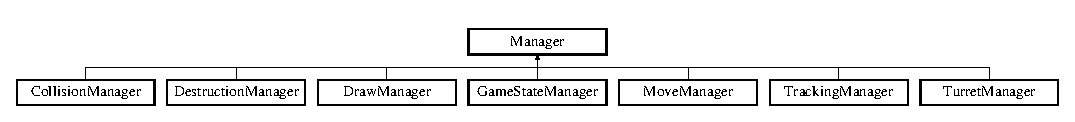
\includegraphics[height=1.185185cm]{classManager}
\end{center}
\end{figure}
\subsection*{Public Member Functions}
\begin{DoxyCompactItemize}
\item 
\hyperlink{classManager_a1658ff9f18e38ccd9cb8b0b371b9c20b}{Manager} ()
\begin{DoxyCompactList}\small\item\em Constructor for \hyperlink{classManager}{Manager}. \end{DoxyCompactList}\item 
virtual \hyperlink{classManager_a322cad25d7007438b3a043ad02253d29}{$\sim$\-Manager} ()
\begin{DoxyCompactList}\small\item\em Destructor. \end{DoxyCompactList}\end{DoxyCompactItemize}


\subsection{Detailed Description}
Abstract-\/\-Base Class of Managers. 

Definition at line 21 of file Manager.\-h.



\subsection{Constructor \& Destructor Documentation}
\hypertarget{classManager_a1658ff9f18e38ccd9cb8b0b371b9c20b}{\index{Manager@{Manager}!Manager@{Manager}}
\index{Manager@{Manager}!Manager@{Manager}}
\subsubsection[{Manager}]{\setlength{\rightskip}{0pt plus 5cm}Manager\-::\-Manager (
\begin{DoxyParamCaption}
{}
\end{DoxyParamCaption}
)}}\label{classManager_a1658ff9f18e38ccd9cb8b0b371b9c20b}


Constructor for \hyperlink{classManager}{Manager}. 

/file \hyperlink{Manager_8cpp}{Manager.\-cpp} /author Daniel Holmes \& Jonathan Gerrand /date 8 September 2014 /brief Implementation for \hyperlink{classManager}{Manager} class 

Definition at line 10 of file Manager.\-cpp.


\begin{DoxyCode}
11 \{
12 
13 \}
\end{DoxyCode}
\hypertarget{classManager_a322cad25d7007438b3a043ad02253d29}{\index{Manager@{Manager}!$\sim$\-Manager@{$\sim$\-Manager}}
\index{$\sim$\-Manager@{$\sim$\-Manager}!Manager@{Manager}}
\subsubsection[{$\sim$\-Manager}]{\setlength{\rightskip}{0pt plus 5cm}Manager\-::$\sim$\-Manager (
\begin{DoxyParamCaption}
{}
\end{DoxyParamCaption}
)\hspace{0.3cm}{\ttfamily [virtual]}}}\label{classManager_a322cad25d7007438b3a043ad02253d29}


Destructor. 



Definition at line 15 of file Manager.\-cpp.


\begin{DoxyCode}
16 \{
17     
18 \}\end{DoxyCode}


The documentation for this class was generated from the following files\-:\begin{DoxyCompactItemize}
\item 
\hyperlink{Manager_8h}{Manager.\-h}\item 
\hyperlink{Manager_8cpp}{Manager.\-cpp}\end{DoxyCompactItemize}

\hypertarget{classManagerTestAssistant}{\section{Manager\-Test\-Assistant Class Reference}
\label{classManagerTestAssistant}\index{Manager\-Test\-Assistant@{Manager\-Test\-Assistant}}
}


{\ttfamily \#include $<$Manager\-Test\-Assistant.\-h$>$}

\subsection*{Public Member Functions}
\begin{DoxyCompactItemize}
\item 
std\-::shared\-\_\-ptr$<$ \hyperlink{classDeletable}{Deletable} $>$ \hyperlink{classManagerTestAssistant_aba7ce13afa76fd729f46247edc4a73a5}{create\-Deletable\-Entity\-Shared\-Pointer} (const \hyperlink{Structures_8h_a6d8f83e710b27d4f86c45f0bb77066e3}{entity\-\_\-type} entity)
\end{DoxyCompactItemize}


\subsection{Detailed Description}


Definition at line 19 of file Manager\-Test\-Assistant.\-h.



\subsection{Member Function Documentation}
\hypertarget{classManagerTestAssistant_aba7ce13afa76fd729f46247edc4a73a5}{\index{Manager\-Test\-Assistant@{Manager\-Test\-Assistant}!create\-Deletable\-Entity\-Shared\-Pointer@{create\-Deletable\-Entity\-Shared\-Pointer}}
\index{create\-Deletable\-Entity\-Shared\-Pointer@{create\-Deletable\-Entity\-Shared\-Pointer}!ManagerTestAssistant@{Manager\-Test\-Assistant}}
\subsubsection[{create\-Deletable\-Entity\-Shared\-Pointer}]{\setlength{\rightskip}{0pt plus 5cm}std\-::shared\-\_\-ptr$<$ {\bf Deletable} $>$ Manager\-Test\-Assistant\-::create\-Deletable\-Entity\-Shared\-Pointer (
\begin{DoxyParamCaption}
\item[{const {\bf entity\-\_\-type}}]{entity}
\end{DoxyParamCaption}
)}}\label{classManagerTestAssistant_aba7ce13afa76fd729f46247edc4a73a5}


Definition at line 11 of file Manager\-Test\-Assistant.\-cpp.



References p1\-\_\-tank.


\begin{DoxyCode}
12 \{
13     \textcolor{keywordflow}{switch}(entity)
14     \{
15         \hyperlink{Structures_8h_a6d8f83e710b27d4f86c45f0bb77066e3a31fa78b2b7dd774f5158a16ef230932e}{p1\_tank}:
16             \{
17                 std::shared\_ptr<Deletable> newTank(\textcolor{keyword}{new} \hyperlink{classTank}{Tank}(10,10,0,\hyperlink{Structures_8h_a6d8f83e710b27d4f86c45f0bb77066e3a31fa78b2b7dd774f5158a16ef230932e}{p1\_tank}));
18                 \textcolor{keywordflow}{return} (newTank);
19             \}
20         \textcolor{keywordflow}{break};
21     \}
22 \}
\end{DoxyCode}


The documentation for this class was generated from the following files\-:\begin{DoxyCompactItemize}
\item 
\hyperlink{ManagerTestAssistant_8h}{Manager\-Test\-Assistant.\-h}\item 
\hyperlink{ManagerTestAssistant_8cpp}{Manager\-Test\-Assistant.\-cpp}\end{DoxyCompactItemize}

\hypertarget{classMine}{\section{Mine Class Reference}
\label{classMine}\index{Mine@{Mine}}
}


Model class for a \hyperlink{classMine}{Mine}.  




{\ttfamily \#include $<$Mine.\-h$>$}

Inheritance diagram for Mine\-:\begin{figure}[H]
\begin{center}
\leavevmode
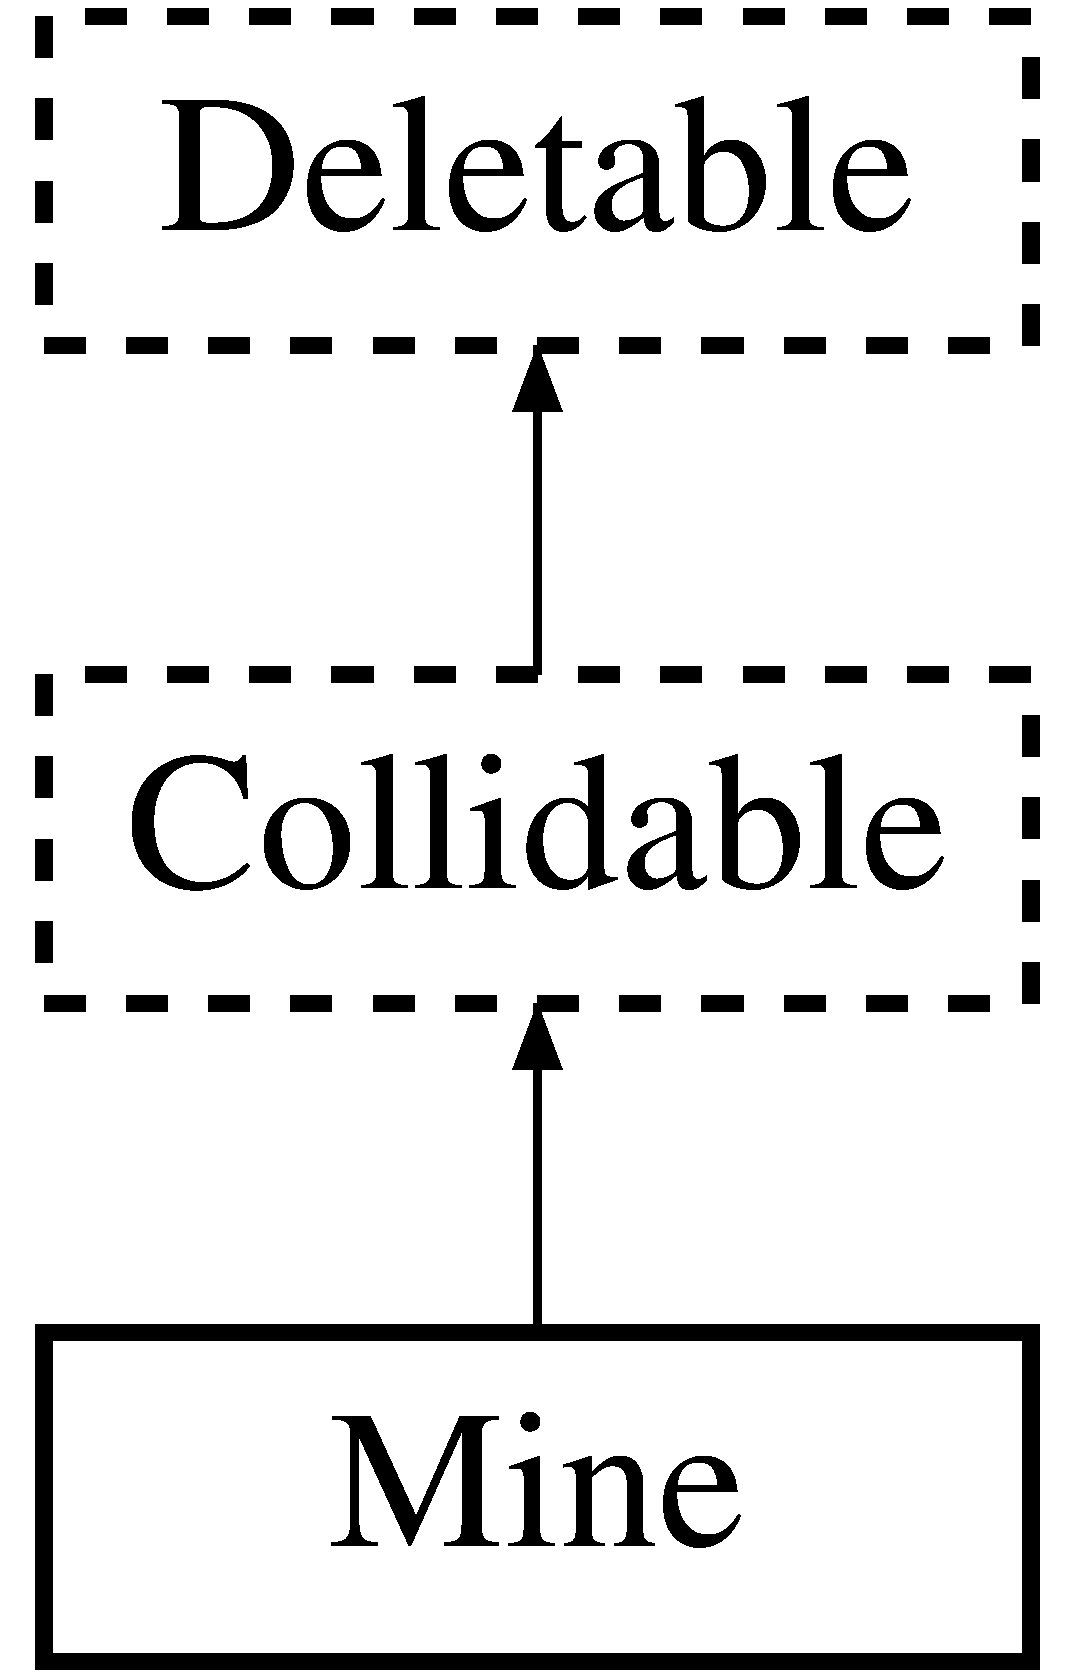
\includegraphics[height=3.000000cm]{classMine}
\end{center}
\end{figure}
\subsection*{Public Member Functions}
\begin{DoxyCompactItemize}
\item 
\hyperlink{classMine_ae3d52389f68d1f458e6240a44cbfd85a}{Mine} (float position\-X, float position\-Y, \hyperlink{Structures_8h_a6d8f83e710b27d4f86c45f0bb77066e3}{entity\-\_\-type} mine\-Owner)
\begin{DoxyCompactList}\small\item\em \hyperlink{classMine}{Mine} entity constructor. \end{DoxyCompactList}\item 
virtual const \hyperlink{Structures_8h_a6d8f83e710b27d4f86c45f0bb77066e3}{entity\-\_\-type} \& \hyperlink{classMine_af435cf100fe7f89e998ec2f7ad40faa1}{get\-Type} () const 
\begin{DoxyCompactList}\small\item\em \hyperlink{classMine}{Mine} is able to provide its identification. \end{DoxyCompactList}\item 
virtual const \hyperlink{structrect__corners}{rect\-\_\-corners} \& \hyperlink{classMine_a36b2ba160a413d45c9743447f075e99e}{get\-Bounding\-Box} ()
\begin{DoxyCompactList}\small\item\em Provide the bounding box for the mine entity. \end{DoxyCompactList}\item 
virtual const \hyperlink{structrect__corners}{rect\-\_\-corners} \& \hyperlink{classMine_a94667c68518d45d9c841501924a83612}{get\-Aligned\-Bounding\-Box} ()
\begin{DoxyCompactList}\small\item\em Get Axis Aligned bounding box of entity. \end{DoxyCompactList}\item 
virtual void \hyperlink{classMine_a859fd28c2c57a37b22ec3b88806f1134}{set\-Unblocked} ()
\begin{DoxyCompactList}\small\item\em This function is not used by the mine. \end{DoxyCompactList}\item 
virtual const int \hyperlink{classMine_acf2add61f1763222f0d1a7333d2b0633}{set\-Blocked} (const \hyperlink{Structures_8h_a6fef29d9424addfa69bdd2a379424896}{blocked\-\_\-status} obstruction\-\_\-type)
\begin{DoxyCompactList}\small\item\em This function is not used by mine. \end{DoxyCompactList}\item 
virtual void \hyperlink{classMine_a3a51fbecfcb177529bee4b7e13dd75e2}{set\-Collided} ()
\begin{DoxyCompactList}\small\item\em Set the colllision state of the mine. \end{DoxyCompactList}\item 
virtual bool const \hyperlink{classMine_aa19d1827e837944d74fe02ad0fbeffc9}{is\-Deleted} ()
\begin{DoxyCompactList}\small\item\em Boolean state of the mine entities life. \end{DoxyCompactList}\item 
virtual const float \hyperlink{classMine_a904342dcd8d13f8489c91ed6ba09ec7b}{get\-Draw\-Position\-X} ()
\begin{DoxyCompactList}\small\item\em Retrieve the \hyperlink{classMine}{Mine} x Position. \end{DoxyCompactList}\item 
virtual const float \hyperlink{classMine_a8abe866b857f781f81b0b3b4e9ef7034}{get\-Draw\-Position\-Y} ()
\begin{DoxyCompactList}\small\item\em Retrieve the \hyperlink{classMine}{Mine} y Position. \end{DoxyCompactList}\item 
virtual const float \hyperlink{classMine_a5b6986a3a3ce5177879359a626cc994b}{get\-Draw\-Rotation} ()
\begin{DoxyCompactList}\small\item\em Recieve the \hyperlink{classMine}{Mine} rotation. \end{DoxyCompactList}\item 
virtual \hyperlink{classMine_abfde171f93b463d81d5b18f767a3a37c}{$\sim$\-Mine} ()
\begin{DoxyCompactList}\small\item\em \hyperlink{classMine}{Mine} object destructor. \end{DoxyCompactList}\end{DoxyCompactItemize}
\subsection*{Private Attributes}
\begin{DoxyCompactItemize}
\item 
\hyperlink{classOrientation}{Orientation} \hyperlink{classMine_ada4e9674ae02b3d3035decc350222aa8}{\-\_\-mine}
\begin{DoxyCompactList}\small\item\em Co-\/cordinate system for \hyperlink{classMine}{Mine} entity. \end{DoxyCompactList}\item 
\hyperlink{Structures_8h_a6d8f83e710b27d4f86c45f0bb77066e3}{entity\-\_\-type} \hyperlink{classMine_a9f780de0af41828d0b03de8ecff36546}{\-\_\-type}
\begin{DoxyCompactList}\small\item\em Enumeration type defining the \hyperlink{classMine}{Mine}. \end{DoxyCompactList}\item 
bool \hyperlink{classMine_a1b68c443899530bad702085dcc52511a}{\-\_\-collided\-Status}
\begin{DoxyCompactList}\small\item\em Collision state of the \hyperlink{classMine}{Mine} entity\-: 1 for collided, 0 for not. \end{DoxyCompactList}\item 
\hyperlink{classSpriteDimensions}{Sprite\-Dimensions} \hyperlink{classMine_a82e6153c008e77eea41dfac4bc665db5}{\-\_\-sprite\-\_\-dimensions}
\begin{DoxyCompactList}\small\item\em \hyperlink{classMine}{Mine} sprite dimensions. \end{DoxyCompactList}\end{DoxyCompactItemize}


\subsection{Detailed Description}
Model class for a \hyperlink{classMine}{Mine}. 

Definition at line 22 of file Mine.\-h.



\subsection{Constructor \& Destructor Documentation}
\hypertarget{classMine_ae3d52389f68d1f458e6240a44cbfd85a}{\index{Mine@{Mine}!Mine@{Mine}}
\index{Mine@{Mine}!Mine@{Mine}}
\subsubsection[{Mine}]{\setlength{\rightskip}{0pt plus 5cm}Mine\-::\-Mine (
\begin{DoxyParamCaption}
\item[{float}]{position\-X, }
\item[{float}]{position\-Y, }
\item[{{\bf entity\-\_\-type}}]{mine\-Owner}
\end{DoxyParamCaption}
)}}\label{classMine_ae3d52389f68d1f458e6240a44cbfd85a}


\hyperlink{classMine}{Mine} entity constructor. 

Throws exceptions if wrong tank owner of position. Initialises private data members 
\begin{DoxyParams}{Parameters}
{\em position\-X} & \-:\-: mine's x position \\
\hline
{\em position\-Y} & \-:\-: mine's y position \\
\hline
{\em mine\-Owner} & \-:\-: either player 1 or player 2 will own the mine \\
\hline
\end{DoxyParams}


Definition at line 17 of file Mine.\-cpp.



References \-\_\-collided\-Status, \-\_\-mine, \-\_\-sprite\-\_\-dimensions, \-\_\-type, Sprite\-Dimensions\-::mine\-\_\-sprite\-\_\-x, Sprite\-Dimensions\-::mine\-\_\-sprite\-\_\-y, p1\-\_\-mine, p2\-\_\-mine, Orientation\-::set\-Height(), and Orientation\-::set\-Width().


\begin{DoxyCode}
17                                                                  :
18     \hyperlink{classMine_ada4e9674ae02b3d3035decc350222aa8}{\_mine}(positionX,positionY,0.0,0.0,0.0, \textcolor{keyword}{false}),
19     \hyperlink{classMine_a82e6153c008e77eea41dfac4bc665db5}{\_sprite\_dimensions}()
20 \{
21     \textcolor{comment}{//Keep Class invariant}
22     \textcolor{keywordflow}{if} ((mineOwner != \hyperlink{Structures_8h_a6d8f83e710b27d4f86c45f0bb77066e3afc52e626787e982ae5d0a747bed6666d}{p1\_mine}) && (mineOwner != \hyperlink{Structures_8h_a6d8f83e710b27d4f86c45f0bb77066e3ada293b37940e64ec2cf6dbd2ae493d2b}{p2\_mine})) \textcolor{keywordflow}{throw} 
      \hyperlink{classInvalidConstructorArgumentsMine}{InvalidConstructorArgumentsMine}();
23     \textcolor{keywordflow}{if} (positionX < 0) \textcolor{keywordflow}{throw} \hyperlink{classInvalidConstructorArgumentsMine}{InvalidConstructorArgumentsMine}();
24     \textcolor{keywordflow}{if} (positionY < 0) \textcolor{keywordflow}{throw} \hyperlink{classInvalidConstructorArgumentsMine}{InvalidConstructorArgumentsMine}();
25 
26     \hyperlink{classMine_ada4e9674ae02b3d3035decc350222aa8}{\_mine}.\hyperlink{classOrientation_a1b5cd490e5bbbe2b8d683be389dbcbbe}{setWidth}(\hyperlink{classMine_a82e6153c008e77eea41dfac4bc665db5}{\_sprite\_dimensions}.
      \hyperlink{classSpriteDimensions_af7f442b00b4a2d9d8b9ad47371a0018f}{mine\_sprite\_x});
27     \hyperlink{classMine_ada4e9674ae02b3d3035decc350222aa8}{\_mine}.\hyperlink{classOrientation_a1adca89bc32128e2ca1cb937357f5006}{setHeight}(\hyperlink{classMine_a82e6153c008e77eea41dfac4bc665db5}{\_sprite\_dimensions}.
      \hyperlink{classSpriteDimensions_a256b5245430fc54ae2cace272260dbe1}{mine\_sprite\_y});
28     \hyperlink{classMine_a9f780de0af41828d0b03de8ecff36546}{\_type} = mineOwner;
29     \hyperlink{classMine_a1b68c443899530bad702085dcc52511a}{\_collidedStatus} = 0;
30 \}
\end{DoxyCode}
\hypertarget{classMine_abfde171f93b463d81d5b18f767a3a37c}{\index{Mine@{Mine}!$\sim$\-Mine@{$\sim$\-Mine}}
\index{$\sim$\-Mine@{$\sim$\-Mine}!Mine@{Mine}}
\subsubsection[{$\sim$\-Mine}]{\setlength{\rightskip}{0pt plus 5cm}Mine\-::$\sim$\-Mine (
\begin{DoxyParamCaption}
{}
\end{DoxyParamCaption}
)\hspace{0.3cm}{\ttfamily [virtual]}}}\label{classMine_abfde171f93b463d81d5b18f767a3a37c}


\hyperlink{classMine}{Mine} object destructor. 



Definition at line 115 of file Mine.\-cpp.


\begin{DoxyCode}
116 \{
117     \textcolor{comment}{//This could possibly be added to}
118 \}
\end{DoxyCode}


\subsection{Member Function Documentation}
\hypertarget{classMine_a94667c68518d45d9c841501924a83612}{\index{Mine@{Mine}!get\-Aligned\-Bounding\-Box@{get\-Aligned\-Bounding\-Box}}
\index{get\-Aligned\-Bounding\-Box@{get\-Aligned\-Bounding\-Box}!Mine@{Mine}}
\subsubsection[{get\-Aligned\-Bounding\-Box}]{\setlength{\rightskip}{0pt plus 5cm}const {\bf rect\-\_\-corners} \& Mine\-::get\-Aligned\-Bounding\-Box (
\begin{DoxyParamCaption}
{}
\end{DoxyParamCaption}
)\hspace{0.3cm}{\ttfamily [virtual]}}}\label{classMine_a94667c68518d45d9c841501924a83612}


Get Axis Aligned bounding box of entity. 

Provide the bounding box for the mine entity.

\begin{DoxyReturn}{Returns}
const \hyperlink{structrect__corners}{rect\-\_\-corners} 
\end{DoxyReturn}


Implements \hyperlink{classCollidable_a6909df57a0915f044d5d967a3be086f3}{Collidable}.



Definition at line 51 of file Mine.\-cpp.



References \-\_\-mine, and Orientation\-::get\-Aligned\-Global\-Bounds().


\begin{DoxyCode}
52 \{
53     \textcolor{keywordflow}{return} \hyperlink{classMine_ada4e9674ae02b3d3035decc350222aa8}{\_mine}.\hyperlink{classOrientation_a5cc606289f774c8561af98d183586199}{getAlignedGlobalBounds}();
54 \}
\end{DoxyCode}
\hypertarget{classMine_a36b2ba160a413d45c9743447f075e99e}{\index{Mine@{Mine}!get\-Bounding\-Box@{get\-Bounding\-Box}}
\index{get\-Bounding\-Box@{get\-Bounding\-Box}!Mine@{Mine}}
\subsubsection[{get\-Bounding\-Box}]{\setlength{\rightskip}{0pt plus 5cm}const {\bf rect\-\_\-corners} \& Mine\-::get\-Bounding\-Box (
\begin{DoxyParamCaption}
{}
\end{DoxyParamCaption}
)\hspace{0.3cm}{\ttfamily [virtual]}}}\label{classMine_a36b2ba160a413d45c9743447f075e99e}


Provide the bounding box for the mine entity. 

\begin{DoxyReturn}{Returns}
const \hyperlink{structrect__corners}{rect\-\_\-corners} 
\end{DoxyReturn}


Implements \hyperlink{classCollidable_a3436effdcd9bea230f4a1aa32b8dd8ab}{Collidable}.



Definition at line 43 of file Mine.\-cpp.



References \-\_\-mine, and Orientation\-::get\-Global\-Bounds().


\begin{DoxyCode}
44 \{
45     \textcolor{keywordflow}{return} \hyperlink{classMine_ada4e9674ae02b3d3035decc350222aa8}{\_mine}.\hyperlink{classOrientation_a950dfe84e548582d8c3c573b5ff5fe42}{getGlobalBounds}();
46 \}
\end{DoxyCode}
\hypertarget{classMine_a904342dcd8d13f8489c91ed6ba09ec7b}{\index{Mine@{Mine}!get\-Draw\-Position\-X@{get\-Draw\-Position\-X}}
\index{get\-Draw\-Position\-X@{get\-Draw\-Position\-X}!Mine@{Mine}}
\subsubsection[{get\-Draw\-Position\-X}]{\setlength{\rightskip}{0pt plus 5cm}const float Mine\-::get\-Draw\-Position\-X (
\begin{DoxyParamCaption}
{}
\end{DoxyParamCaption}
)\hspace{0.3cm}{\ttfamily [virtual]}}}\label{classMine_a904342dcd8d13f8489c91ed6ba09ec7b}


Retrieve the \hyperlink{classMine}{Mine} x Position. 



Implements \hyperlink{classDeletable_ac14ea0c5986d50ba3ba454f89c87b8fe}{Deletable}.



Definition at line 91 of file Mine.\-cpp.



References \-\_\-mine, and Orientation\-::get\-Origin\-X().


\begin{DoxyCode}
92 \{
93     \textcolor{keywordflow}{return} \hyperlink{classMine_ada4e9674ae02b3d3035decc350222aa8}{\_mine}.\hyperlink{classOrientation_a4d6b853f2ac00965d29e5bc36b94c949}{getOriginX}();
94 \}
\end{DoxyCode}
\hypertarget{classMine_a8abe866b857f781f81b0b3b4e9ef7034}{\index{Mine@{Mine}!get\-Draw\-Position\-Y@{get\-Draw\-Position\-Y}}
\index{get\-Draw\-Position\-Y@{get\-Draw\-Position\-Y}!Mine@{Mine}}
\subsubsection[{get\-Draw\-Position\-Y}]{\setlength{\rightskip}{0pt plus 5cm}const float Mine\-::get\-Draw\-Position\-Y (
\begin{DoxyParamCaption}
{}
\end{DoxyParamCaption}
)\hspace{0.3cm}{\ttfamily [virtual]}}}\label{classMine_a8abe866b857f781f81b0b3b4e9ef7034}


Retrieve the \hyperlink{classMine}{Mine} y Position. 



Implements \hyperlink{classDeletable_a2a88d7e40c56902a3d3d8f668e9d126d}{Deletable}.



Definition at line 99 of file Mine.\-cpp.



References \-\_\-mine, and Orientation\-::get\-Origin\-Y().


\begin{DoxyCode}
100 \{
101     \textcolor{keywordflow}{return} \hyperlink{classMine_ada4e9674ae02b3d3035decc350222aa8}{\_mine}.\hyperlink{classOrientation_ae60c88b0525d6e536a1a068d3a99f74c}{getOriginY}();
102 \}
\end{DoxyCode}
\hypertarget{classMine_a5b6986a3a3ce5177879359a626cc994b}{\index{Mine@{Mine}!get\-Draw\-Rotation@{get\-Draw\-Rotation}}
\index{get\-Draw\-Rotation@{get\-Draw\-Rotation}!Mine@{Mine}}
\subsubsection[{get\-Draw\-Rotation}]{\setlength{\rightskip}{0pt plus 5cm}const float Mine\-::get\-Draw\-Rotation (
\begin{DoxyParamCaption}
{}
\end{DoxyParamCaption}
)\hspace{0.3cm}{\ttfamily [virtual]}}}\label{classMine_a5b6986a3a3ce5177879359a626cc994b}


Recieve the \hyperlink{classMine}{Mine} rotation. 



Implements \hyperlink{classDeletable_ad7061a6bef3efce030aa5abbc7646d47}{Deletable}.



Definition at line 107 of file Mine.\-cpp.



References \-\_\-mine, and Orientation\-::get\-Rotation().


\begin{DoxyCode}
108 \{
109     \textcolor{keywordflow}{return} \hyperlink{classMine_ada4e9674ae02b3d3035decc350222aa8}{\_mine}.\hyperlink{classOrientation_ab3568e037a7dc7799d557f2bc6a3cf7d}{getRotation}();
110 \}
\end{DoxyCode}
\hypertarget{classMine_af435cf100fe7f89e998ec2f7ad40faa1}{\index{Mine@{Mine}!get\-Type@{get\-Type}}
\index{get\-Type@{get\-Type}!Mine@{Mine}}
\subsubsection[{get\-Type}]{\setlength{\rightskip}{0pt plus 5cm}const {\bf entity\-\_\-type} \& Mine\-::get\-Type (
\begin{DoxyParamCaption}
{}
\end{DoxyParamCaption}
) const\hspace{0.3cm}{\ttfamily [virtual]}}}\label{classMine_af435cf100fe7f89e998ec2f7ad40faa1}


\hyperlink{classMine}{Mine} is able to provide its identification. 

\begin{DoxyReturn}{Returns}
const entity\-\_\-type 
\end{DoxyReturn}


Implements \hyperlink{classDeletable_af8a0208abc297180873692f4215fe50f}{Deletable}.



Definition at line 35 of file Mine.\-cpp.



References \-\_\-type.



Referenced by T\-E\-S\-T().


\begin{DoxyCode}
36 \{
37     \textcolor{keywordflow}{return} \hyperlink{classMine_a9f780de0af41828d0b03de8ecff36546}{\_type};
38 \}
\end{DoxyCode}
\hypertarget{classMine_aa19d1827e837944d74fe02ad0fbeffc9}{\index{Mine@{Mine}!is\-Deleted@{is\-Deleted}}
\index{is\-Deleted@{is\-Deleted}!Mine@{Mine}}
\subsubsection[{is\-Deleted}]{\setlength{\rightskip}{0pt plus 5cm}const bool Mine\-::is\-Deleted (
\begin{DoxyParamCaption}
{}
\end{DoxyParamCaption}
)\hspace{0.3cm}{\ttfamily [virtual]}}}\label{classMine_aa19d1827e837944d74fe02ad0fbeffc9}


Boolean state of the mine entities life. 

Boolean state of the mine entities. 

Implements \hyperlink{classDeletable_a6572440c291077cf52bf21288c6cd25c}{Deletable}.



Definition at line 83 of file Mine.\-cpp.



References \-\_\-collided\-Status.



Referenced by T\-E\-S\-T().


\begin{DoxyCode}
84 \{
85     \textcolor{keywordflow}{return} \hyperlink{classMine_a1b68c443899530bad702085dcc52511a}{\_collidedStatus};
86 \}
\end{DoxyCode}
\hypertarget{classMine_acf2add61f1763222f0d1a7333d2b0633}{\index{Mine@{Mine}!set\-Blocked@{set\-Blocked}}
\index{set\-Blocked@{set\-Blocked}!Mine@{Mine}}
\subsubsection[{set\-Blocked}]{\setlength{\rightskip}{0pt plus 5cm}const int Mine\-::set\-Blocked (
\begin{DoxyParamCaption}
\item[{const {\bf blocked\-\_\-status}}]{obstruction\-\_\-type}
\end{DoxyParamCaption}
)\hspace{0.3cm}{\ttfamily [virtual]}}}\label{classMine_acf2add61f1763222f0d1a7333d2b0633}


This function is not used by mine. 

\begin{DoxyReturn}{Returns}
const int 
\end{DoxyReturn}


Implements \hyperlink{classCollidable_a6d312198ba82d26b5e360733bb87a2f0}{Collidable}.



Definition at line 59 of file Mine.\-cpp.


\begin{DoxyCode}
60 \{
61     \textcolor{keywordflow}{return} 1;
62 \}
\end{DoxyCode}
\hypertarget{classMine_a3a51fbecfcb177529bee4b7e13dd75e2}{\index{Mine@{Mine}!set\-Collided@{set\-Collided}}
\index{set\-Collided@{set\-Collided}!Mine@{Mine}}
\subsubsection[{set\-Collided}]{\setlength{\rightskip}{0pt plus 5cm}void Mine\-::set\-Collided (
\begin{DoxyParamCaption}
{}
\end{DoxyParamCaption}
)\hspace{0.3cm}{\ttfamily [virtual]}}}\label{classMine_a3a51fbecfcb177529bee4b7e13dd75e2}


Set the colllision state of the mine. 



Implements \hyperlink{classCollidable_a5ea0417bea000712171bbe5531705082}{Collidable}.



Definition at line 75 of file Mine.\-cpp.



References \-\_\-collided\-Status.



Referenced by T\-E\-S\-T().


\begin{DoxyCode}
76 \{
77     \hyperlink{classMine_a1b68c443899530bad702085dcc52511a}{\_collidedStatus} = 1;
78 \}
\end{DoxyCode}
\hypertarget{classMine_a859fd28c2c57a37b22ec3b88806f1134}{\index{Mine@{Mine}!set\-Unblocked@{set\-Unblocked}}
\index{set\-Unblocked@{set\-Unblocked}!Mine@{Mine}}
\subsubsection[{set\-Unblocked}]{\setlength{\rightskip}{0pt plus 5cm}void Mine\-::set\-Unblocked (
\begin{DoxyParamCaption}
{}
\end{DoxyParamCaption}
)\hspace{0.3cm}{\ttfamily [virtual]}}}\label{classMine_a859fd28c2c57a37b22ec3b88806f1134}


This function is not used by the mine. 

This function is not used by mine. 

Implements \hyperlink{classCollidable_a817d864d0640bc6bcb13bbecf14ddf31}{Collidable}.



Definition at line 67 of file Mine.\-cpp.


\begin{DoxyCode}
68 \{
69     \textcolor{comment}{//This should be thought about and worked aound}
70 \}
\end{DoxyCode}


\subsection{Member Data Documentation}
\hypertarget{classMine_a1b68c443899530bad702085dcc52511a}{\index{Mine@{Mine}!\-\_\-collided\-Status@{\-\_\-collided\-Status}}
\index{\-\_\-collided\-Status@{\-\_\-collided\-Status}!Mine@{Mine}}
\subsubsection[{\-\_\-collided\-Status}]{\setlength{\rightskip}{0pt plus 5cm}bool Mine\-::\-\_\-collided\-Status\hspace{0.3cm}{\ttfamily [private]}}}\label{classMine_a1b68c443899530bad702085dcc52511a}


Collision state of the \hyperlink{classMine}{Mine} entity\-: 1 for collided, 0 for not. 



Definition at line 59 of file Mine.\-h.



Referenced by is\-Deleted(), Mine(), and set\-Collided().

\hypertarget{classMine_ada4e9674ae02b3d3035decc350222aa8}{\index{Mine@{Mine}!\-\_\-mine@{\-\_\-mine}}
\index{\-\_\-mine@{\-\_\-mine}!Mine@{Mine}}
\subsubsection[{\-\_\-mine}]{\setlength{\rightskip}{0pt plus 5cm}{\bf Orientation} Mine\-::\-\_\-mine\hspace{0.3cm}{\ttfamily [private]}}}\label{classMine_ada4e9674ae02b3d3035decc350222aa8}


Co-\/cordinate system for \hyperlink{classMine}{Mine} entity. 



Definition at line 55 of file Mine.\-h.



Referenced by get\-Aligned\-Bounding\-Box(), get\-Bounding\-Box(), get\-Draw\-Position\-X(), get\-Draw\-Position\-Y(), get\-Draw\-Rotation(), and Mine().

\hypertarget{classMine_a82e6153c008e77eea41dfac4bc665db5}{\index{Mine@{Mine}!\-\_\-sprite\-\_\-dimensions@{\-\_\-sprite\-\_\-dimensions}}
\index{\-\_\-sprite\-\_\-dimensions@{\-\_\-sprite\-\_\-dimensions}!Mine@{Mine}}
\subsubsection[{\-\_\-sprite\-\_\-dimensions}]{\setlength{\rightskip}{0pt plus 5cm}{\bf Sprite\-Dimensions} Mine\-::\-\_\-sprite\-\_\-dimensions\hspace{0.3cm}{\ttfamily [private]}}}\label{classMine_a82e6153c008e77eea41dfac4bc665db5}


\hyperlink{classMine}{Mine} sprite dimensions. 



Definition at line 61 of file Mine.\-h.



Referenced by Mine().

\hypertarget{classMine_a9f780de0af41828d0b03de8ecff36546}{\index{Mine@{Mine}!\-\_\-type@{\-\_\-type}}
\index{\-\_\-type@{\-\_\-type}!Mine@{Mine}}
\subsubsection[{\-\_\-type}]{\setlength{\rightskip}{0pt plus 5cm}{\bf entity\-\_\-type} Mine\-::\-\_\-type\hspace{0.3cm}{\ttfamily [private]}}}\label{classMine_a9f780de0af41828d0b03de8ecff36546}


Enumeration type defining the \hyperlink{classMine}{Mine}. 



Definition at line 57 of file Mine.\-h.



Referenced by get\-Type(), and Mine().



The documentation for this class was generated from the following files\-:\begin{DoxyCompactItemize}
\item 
\hyperlink{Mine_8h}{Mine.\-h}\item 
\hyperlink{Mine_8cpp}{Mine.\-cpp}\end{DoxyCompactItemize}

\hypertarget{classMissile}{\section{Missile Class Reference}
\label{classMissile}\index{Missile@{Missile}}
}


\hyperlink{classMissile}{Missile} Class implementation.  




{\ttfamily \#include $<$Missile.\-h$>$}

Inheritance diagram for Missile\-:\begin{figure}[H]
\begin{center}
\leavevmode
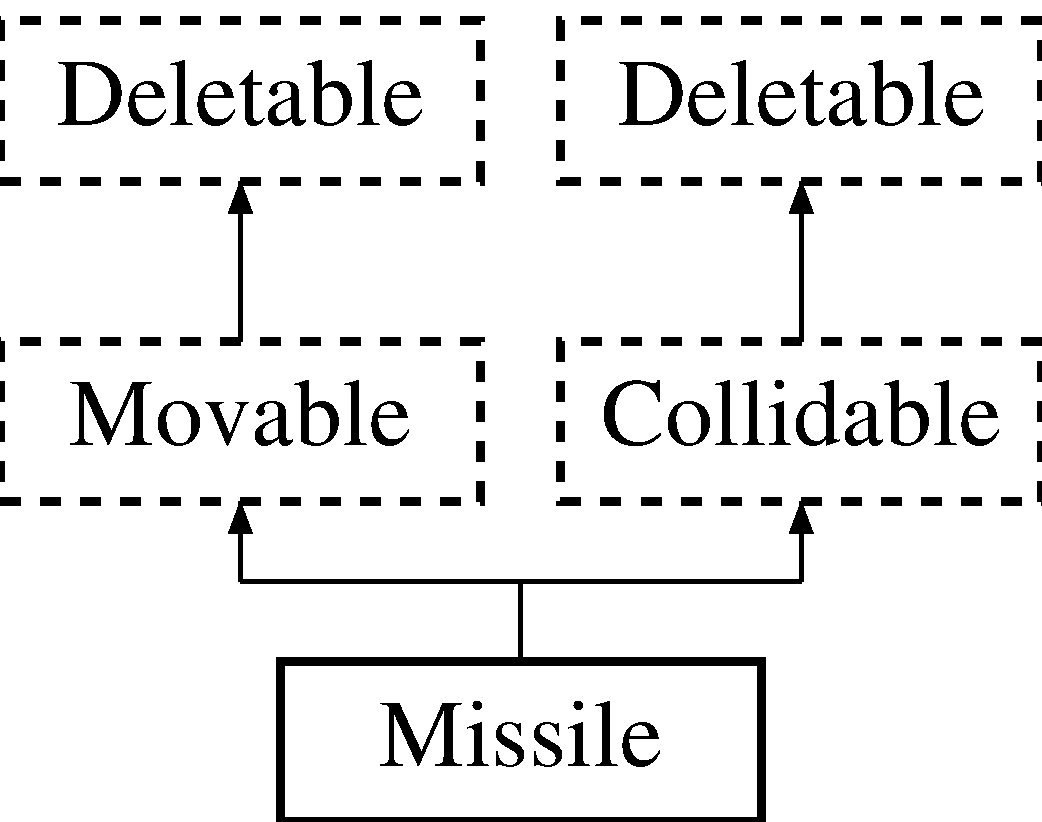
\includegraphics[height=3.000000cm]{classMissile}
\end{center}
\end{figure}
\subsection*{Public Member Functions}
\begin{DoxyCompactItemize}
\item 
\hyperlink{classMissile_a2f930ea9ba87704d2ba75b0299f698c2}{Missile} (float position\-X, float position\-Y, float rotation, \hyperlink{Structures_8h_a6d8f83e710b27d4f86c45f0bb77066e3}{entity\-\_\-type} missile\-Owner)
\begin{DoxyCompactList}\small\item\em \hyperlink{classMissile}{Missile} object constructor. \end{DoxyCompactList}\item 
virtual const \hyperlink{Structures_8h_a6d8f83e710b27d4f86c45f0bb77066e3}{entity\-\_\-type} \& \hyperlink{classMissile_a67874a53d50f63065bf1f63803558513}{get\-Type} () const 
\begin{DoxyCompactList}\small\item\em Return the ownership and type of the \hyperlink{classMissile}{Missile} entity. \end{DoxyCompactList}\item 
virtual void \hyperlink{classMissile_a4b6a45a5129b97a6e5383123dffab0c3}{move\-Forward} ()
\begin{DoxyCompactList}\small\item\em Forward movement for a missile entity. \end{DoxyCompactList}\item 
virtual void \hyperlink{classMissile_a8d8348b91961ff0c163d7d24bd9599a8}{move\-Backward} ()
\begin{DoxyCompactList}\small\item\em Backward movement for a missile entity. \end{DoxyCompactList}\item 
virtual void \hyperlink{classMissile_a1c7ed80bd656b0af5b3872f4225978e3}{rotate\-Left} ()
\begin{DoxyCompactList}\small\item\em Left rotation for a missile entity. \end{DoxyCompactList}\item 
virtual void \hyperlink{classMissile_aeccfdf94a02fa86545296f4c38857ef8}{rotate\-Right} ()
\begin{DoxyCompactList}\small\item\em Right rotation for a missile entity. \end{DoxyCompactList}\item 
virtual const \hyperlink{structrect__corners}{rect\-\_\-corners} \& \hyperlink{classMissile_a6f9a14b7e2a2041fbccb566bf2a3b469}{get\-Bounding\-Box} ()
\begin{DoxyCompactList}\small\item\em Provide the bounding box for the missile entity. \end{DoxyCompactList}\item 
virtual const \hyperlink{structrect__corners}{rect\-\_\-corners} \& \hyperlink{classMissile_af2a9b1f8503cc2d322f5ab6ea788d393}{get\-Aligned\-Bounding\-Box} ()
\begin{DoxyCompactList}\small\item\em Get Axis Aligned bounding box of entity. \end{DoxyCompactList}\item 
virtual const int \hyperlink{classMissile_a4f6e73f8d9f9723a777875efcb9edfa7}{set\-Blocked} (const \hyperlink{Structures_8h_a6fef29d9424addfa69bdd2a379424896}{blocked\-\_\-status} obstruction\-\_\-type)
\begin{DoxyCompactList}\small\item\em Instruct the missile entity that it cannot move along its trajectory. \end{DoxyCompactList}\item 
virtual void \hyperlink{classMissile_af66d762c4401061f64bcf9b46343c967}{set\-Unblocked} ()
\begin{DoxyCompactList}\small\item\em Instruct the missile entity that it can move. \end{DoxyCompactList}\item 
virtual void \hyperlink{classMissile_a1a27cc48265f34e3298c780c37ca8a0e}{set\-Collided} ()
\begin{DoxyCompactList}\small\item\em Instruct the missile entity that it has collided with another object. \end{DoxyCompactList}\item 
virtual const \hyperlink{Structures_8h_a6fef29d9424addfa69bdd2a379424896}{blocked\-\_\-status} \hyperlink{classMissile_a2c86874bf5e6bde8cb97f4ed1a07c3ea}{is\-Blocked} ()
\begin{DoxyCompactList}\small\item\em Determine the blocked state of the missile entity. \end{DoxyCompactList}\item 
virtual bool const \hyperlink{classMissile_a96c1240f08fed605ff9e908a0bea50e4}{is\-Deleted} ()
\begin{DoxyCompactList}\small\item\em Boolean state of the missile entity's life. \end{DoxyCompactList}\item 
virtual const float \hyperlink{classMissile_a8e8d526d7578cfbabbd5bf1bdb9727bc}{get\-Draw\-Position\-X} ()
\begin{DoxyCompactList}\small\item\em Retrieve the missile x Position. \end{DoxyCompactList}\item 
virtual const float \hyperlink{classMissile_ad609bee2bfaf610824f32c15430fa6d8}{get\-Draw\-Position\-Y} ()
\begin{DoxyCompactList}\small\item\em Retrieve the missile y Position. \end{DoxyCompactList}\item 
virtual const float \hyperlink{classMissile_ab606b0b4f38c821063f210625f926374}{get\-Draw\-Rotation} ()
\begin{DoxyCompactList}\small\item\em Receive the missile rotation. \end{DoxyCompactList}\item 
virtual void \hyperlink{classMissile_a5bff45d0243e353acdf610fdade02bb0}{set\-Movement\-Direction} (const \hyperlink{Structures_8h_a0d0b88f27f3adf9452879b5d9f829026}{movement\-\_\-direction} Movement\-\_\-input)
\begin{DoxyCompactList}\small\item\em Set the movement direction of the entity. \end{DoxyCompactList}\item 
virtual \hyperlink{classMissile_ad42379e48a46ec3556056f98ce8bd912}{$\sim$\-Missile} ()
\begin{DoxyCompactList}\small\item\em \hyperlink{classMissile}{Missile} object destructor. \end{DoxyCompactList}\end{DoxyCompactItemize}
\subsection*{Private Attributes}
\begin{DoxyCompactItemize}
\item 
\hyperlink{Structures_8h_a6fef29d9424addfa69bdd2a379424896}{blocked\-\_\-status} \hyperlink{classMissile_a34065d77889cdf8ac998d83dc0b3a242}{\-\_\-blocked\-Status}
\begin{DoxyCompactList}\small\item\em Movability of the \hyperlink{classMissile}{Missile} entity\-: 1 for blocked, 0 for free. \end{DoxyCompactList}\item 
bool \hyperlink{classMissile_a52e8aaac3c5db45c8d4c1ac74d001f57}{\-\_\-collided\-Status}
\begin{DoxyCompactList}\small\item\em Collision state of the \hyperlink{classMissile}{Missile} Entity\-: 1 for collided, 0 for not. \end{DoxyCompactList}\item 
float \hyperlink{classMissile_acd500cfc21ada9701b059cb4a77a5c96}{\-\_\-rotation}
\begin{DoxyCompactList}\small\item\em The angle of rotation for the \hyperlink{classMissile}{Missile} entity. \end{DoxyCompactList}\item 
\hyperlink{classOrientation}{Orientation} \hyperlink{classMissile_ae8ef6a656e69ac376dbc0db1b7153250}{\-\_\-missile}
\begin{DoxyCompactList}\small\item\em S\-F\-M\-L Co-\/ordinate system for the \hyperlink{classMissile}{Missile}. \end{DoxyCompactList}\item 
\hyperlink{Structures_8h_a6d8f83e710b27d4f86c45f0bb77066e3}{entity\-\_\-type} \hyperlink{classMissile_a2cbcb75f29640ba706e64cb620a7c6a7}{\-\_\-type}
\begin{DoxyCompactList}\small\item\em Enumeration type defining the \hyperlink{classMissile}{Missile}. \end{DoxyCompactList}\item 
\hyperlink{classSpriteDimensions}{Sprite\-Dimensions} \hyperlink{classMissile_a97a02568096e4900a56067e2f2b346fc}{\-\_\-sprite\-\_\-dimensions}
\begin{DoxyCompactList}\small\item\em \hyperlink{classMissile}{Missile} Sprite dimensions. \end{DoxyCompactList}\item 
int \hyperlink{classMissile_afc61d2903e66bc48c42bb70e7ddd55d8}{\-\_\-rebound\-\_\-lives}
\begin{DoxyCompactList}\small\item\em Defines the number of times the \hyperlink{classMissile}{Missile} can rebound off barriers. \end{DoxyCompactList}\end{DoxyCompactItemize}
\subsection*{Additional Inherited Members}


\subsection{Detailed Description}
\hyperlink{classMissile}{Missile} Class implementation. 

Entity Class representing the \hyperlink{classMissile}{Missile} in the game world.

This class possesses multiple interfaces for interaction with various managers and forms part of the basic model entities 

Definition at line 26 of file Missile.\-h.



\subsection{Constructor \& Destructor Documentation}
\hypertarget{classMissile_a2f930ea9ba87704d2ba75b0299f698c2}{\index{Missile@{Missile}!Missile@{Missile}}
\index{Missile@{Missile}!Missile@{Missile}}
\subsubsection[{Missile}]{\setlength{\rightskip}{0pt plus 5cm}Missile\-::\-Missile (
\begin{DoxyParamCaption}
\item[{float}]{position\-X, }
\item[{float}]{position\-Y, }
\item[{float}]{rotation, }
\item[{{\bf entity\-\_\-type}}]{missile\-Owner}
\end{DoxyParamCaption}
)}}\label{classMissile_a2f930ea9ba87704d2ba75b0299f698c2}


\hyperlink{classMissile}{Missile} object constructor. 



Definition at line 15 of file Missile.\-cpp.



References \-\_\-blocked\-Status, \-\_\-collided\-Status, \-\_\-missile, \-\_\-rebound\-\_\-lives, \-\_\-sprite\-\_\-dimensions, \-\_\-type, Orientation\-::get\-Origin\-X(), Orientation\-::get\-Origin\-Y(), Orientation\-::get\-Rotation(), Sprite\-Dimensions\-::missile\-\_\-sprite\-\_\-x, Sprite\-Dimensions\-::missile\-\_\-sprite\-\_\-y, p1\-\_\-missile, p2\-\_\-missile, Orientation\-::set\-Height(), Orientation\-::set\-Width(), turret\-\_\-missile, and unblocked.


\begin{DoxyCode}
15                                                                                           :
16 
17     \hyperlink{classMissile_acd500cfc21ada9701b059cb4a77a5c96}{\_rotation}(rotation),
18     \hyperlink{classMissile_a2cbcb75f29640ba706e64cb620a7c6a7}{\_type}(missileOwner),
19     \hyperlink{classMissile_ae8ef6a656e69ac376dbc0db1b7153250}{\_missile}(positionX,positionY,0,0,rotation, \textcolor{keyword}{false}),
20     \hyperlink{classMissile_a97a02568096e4900a56067e2f2b346fc}{\_sprite\_dimensions}()
21 \{
22     \textcolor{comment}{//Error input checking}
23     \textcolor{keywordflow}{if} (\hyperlink{classMissile_ae8ef6a656e69ac376dbc0db1b7153250}{\_missile}.\hyperlink{classOrientation_a4d6b853f2ac00965d29e5bc36b94c949}{getOriginX}() < 0) \textcolor{keywordflow}{throw} 
      \hyperlink{classInvalidConstructorArgumentsMissile}{InvalidConstructorArgumentsMissile}();
24     \textcolor{keywordflow}{if} (\hyperlink{classMissile_ae8ef6a656e69ac376dbc0db1b7153250}{\_missile}.\hyperlink{classOrientation_ae60c88b0525d6e536a1a068d3a99f74c}{getOriginY}() < 0) \textcolor{keywordflow}{throw} 
      \hyperlink{classInvalidConstructorArgumentsMissile}{InvalidConstructorArgumentsMissile}();
25     \textcolor{keywordflow}{if} (\hyperlink{classMissile_ae8ef6a656e69ac376dbc0db1b7153250}{\_missile}.\hyperlink{classOrientation_ab3568e037a7dc7799d557f2bc6a3cf7d}{getRotation}() < 0) \textcolor{keywordflow}{throw} 
      \hyperlink{classInvalidConstructorArgumentsMissile}{InvalidConstructorArgumentsMissile}();
26     \textcolor{keywordflow}{if} ((\hyperlink{classMissile_a2cbcb75f29640ba706e64cb620a7c6a7}{\_type} != \hyperlink{Structures_8h_a6d8f83e710b27d4f86c45f0bb77066e3af89bc631e9b0140ed004b5ce2db5330c}{p1\_missile}) && (\hyperlink{classMissile_a2cbcb75f29640ba706e64cb620a7c6a7}{\_type} != \hyperlink{Structures_8h_a6d8f83e710b27d4f86c45f0bb77066e3a47100170e5852d632dfe65582a18256d}{p2\_missile}) && (
      \hyperlink{classMissile_a2cbcb75f29640ba706e64cb620a7c6a7}{\_type} != \hyperlink{Structures_8h_a6d8f83e710b27d4f86c45f0bb77066e3a8f552a1e495ced5aa8775faa1b6a757b}{turret\_missile})) \textcolor{keywordflow}{throw} 
      \hyperlink{classInvalidConstructorArgumentsMissile}{InvalidConstructorArgumentsMissile}();
27 
28     \hyperlink{classMissile_ae8ef6a656e69ac376dbc0db1b7153250}{\_missile}.\hyperlink{classOrientation_a1b5cd490e5bbbe2b8d683be389dbcbbe}{setWidth}(\hyperlink{classMissile_a97a02568096e4900a56067e2f2b346fc}{\_sprite\_dimensions}.
      \hyperlink{classSpriteDimensions_a0c406c32caf5ea7841c763100dd83ecf}{missile\_sprite\_x});
29     \hyperlink{classMissile_ae8ef6a656e69ac376dbc0db1b7153250}{\_missile}.\hyperlink{classOrientation_a1adca89bc32128e2ca1cb937357f5006}{setHeight}(\hyperlink{classMissile_a97a02568096e4900a56067e2f2b346fc}{\_sprite\_dimensions}.
      \hyperlink{classSpriteDimensions_adcf501d11ae383d24cbbe5b526585f86}{missile\_sprite\_y});
30     \hyperlink{classMissile_a34065d77889cdf8ac998d83dc0b3a242}{\_blockedStatus} = \hyperlink{Structures_8h_a6fef29d9424addfa69bdd2a379424896a1596fbf6035468467c790068b609ced3}{unblocked};
31     \hyperlink{classMissile_a52e8aaac3c5db45c8d4c1ac74d001f57}{\_collidedStatus} = 0;
32     \hyperlink{classMissile_afc61d2903e66bc48c42bb70e7ddd55d8}{\_rebound\_lives} = 7;
33 \}
\end{DoxyCode}
\hypertarget{classMissile_ad42379e48a46ec3556056f98ce8bd912}{\index{Missile@{Missile}!$\sim$\-Missile@{$\sim$\-Missile}}
\index{$\sim$\-Missile@{$\sim$\-Missile}!Missile@{Missile}}
\subsubsection[{$\sim$\-Missile}]{\setlength{\rightskip}{0pt plus 5cm}Missile\-::$\sim$\-Missile (
\begin{DoxyParamCaption}
{}
\end{DoxyParamCaption}
)\hspace{0.3cm}{\ttfamily [virtual]}}}\label{classMissile_ad42379e48a46ec3556056f98ce8bd912}


\hyperlink{classMissile}{Missile} object destructor. 



Definition at line 141 of file Missile.\-cpp.


\begin{DoxyCode}
142 \{
143     \textcolor{comment}{//Consider adding something here}
144 \}
\end{DoxyCode}


\subsection{Member Function Documentation}
\hypertarget{classMissile_af2a9b1f8503cc2d322f5ab6ea788d393}{\index{Missile@{Missile}!get\-Aligned\-Bounding\-Box@{get\-Aligned\-Bounding\-Box}}
\index{get\-Aligned\-Bounding\-Box@{get\-Aligned\-Bounding\-Box}!Missile@{Missile}}
\subsubsection[{get\-Aligned\-Bounding\-Box}]{\setlength{\rightskip}{0pt plus 5cm}const {\bf rect\-\_\-corners} \& Missile\-::get\-Aligned\-Bounding\-Box (
\begin{DoxyParamCaption}
{}
\end{DoxyParamCaption}
)\hspace{0.3cm}{\ttfamily [virtual]}}}\label{classMissile_af2a9b1f8503cc2d322f5ab6ea788d393}


Get Axis Aligned bounding box of entity. 



Implements \hyperlink{classCollidable_a6909df57a0915f044d5d967a3be086f3}{Collidable}.



Definition at line 78 of file Missile.\-cpp.



References \-\_\-missile, and Orientation\-::get\-Aligned\-Global\-Bounds().


\begin{DoxyCode}
79 \{
80     \textcolor{keywordflow}{return} \hyperlink{classMissile_ae8ef6a656e69ac376dbc0db1b7153250}{\_missile}.\hyperlink{classOrientation_a5cc606289f774c8561af98d183586199}{getAlignedGlobalBounds}();
81 \}
\end{DoxyCode}
\hypertarget{classMissile_a6f9a14b7e2a2041fbccb566bf2a3b469}{\index{Missile@{Missile}!get\-Bounding\-Box@{get\-Bounding\-Box}}
\index{get\-Bounding\-Box@{get\-Bounding\-Box}!Missile@{Missile}}
\subsubsection[{get\-Bounding\-Box}]{\setlength{\rightskip}{0pt plus 5cm}const {\bf rect\-\_\-corners} \& Missile\-::get\-Bounding\-Box (
\begin{DoxyParamCaption}
{}
\end{DoxyParamCaption}
)\hspace{0.3cm}{\ttfamily [virtual]}}}\label{classMissile_a6f9a14b7e2a2041fbccb566bf2a3b469}


Provide the bounding box for the missile entity. 



Implements \hyperlink{classCollidable_a3436effdcd9bea230f4a1aa32b8dd8ab}{Collidable}.



Definition at line 73 of file Missile.\-cpp.



References \-\_\-missile, and Orientation\-::get\-Global\-Bounds().


\begin{DoxyCode}
74 \{
75     \textcolor{keywordflow}{return} \hyperlink{classMissile_ae8ef6a656e69ac376dbc0db1b7153250}{\_missile}.\hyperlink{classOrientation_a950dfe84e548582d8c3c573b5ff5fe42}{getGlobalBounds}();
76 \}
\end{DoxyCode}
\hypertarget{classMissile_a8e8d526d7578cfbabbd5bf1bdb9727bc}{\index{Missile@{Missile}!get\-Draw\-Position\-X@{get\-Draw\-Position\-X}}
\index{get\-Draw\-Position\-X@{get\-Draw\-Position\-X}!Missile@{Missile}}
\subsubsection[{get\-Draw\-Position\-X}]{\setlength{\rightskip}{0pt plus 5cm}const float Missile\-::get\-Draw\-Position\-X (
\begin{DoxyParamCaption}
{}
\end{DoxyParamCaption}
)\hspace{0.3cm}{\ttfamily [virtual]}}}\label{classMissile_a8e8d526d7578cfbabbd5bf1bdb9727bc}


Retrieve the missile x Position. 

Retrieve the \hyperlink{classMissile}{Missile} x Position. 

Implements \hyperlink{classDeletable_ac14ea0c5986d50ba3ba454f89c87b8fe}{Deletable}.



Definition at line 116 of file Missile.\-cpp.



References \-\_\-missile, and Orientation\-::get\-Origin\-X().



Referenced by T\-E\-S\-T().


\begin{DoxyCode}
117 \{
118     \textcolor{keywordflow}{return} \hyperlink{classMissile_ae8ef6a656e69ac376dbc0db1b7153250}{\_missile}.\hyperlink{classOrientation_a4d6b853f2ac00965d29e5bc36b94c949}{getOriginX}();
119 \}
\end{DoxyCode}
\hypertarget{classMissile_ad609bee2bfaf610824f32c15430fa6d8}{\index{Missile@{Missile}!get\-Draw\-Position\-Y@{get\-Draw\-Position\-Y}}
\index{get\-Draw\-Position\-Y@{get\-Draw\-Position\-Y}!Missile@{Missile}}
\subsubsection[{get\-Draw\-Position\-Y}]{\setlength{\rightskip}{0pt plus 5cm}const float Missile\-::get\-Draw\-Position\-Y (
\begin{DoxyParamCaption}
{}
\end{DoxyParamCaption}
)\hspace{0.3cm}{\ttfamily [virtual]}}}\label{classMissile_ad609bee2bfaf610824f32c15430fa6d8}


Retrieve the missile y Position. 

Retrieve the \hyperlink{classMissile}{Missile} y Position. 

Implements \hyperlink{classDeletable_a2a88d7e40c56902a3d3d8f668e9d126d}{Deletable}.



Definition at line 122 of file Missile.\-cpp.



References \-\_\-missile, and Orientation\-::get\-Origin\-Y().



Referenced by T\-E\-S\-T().


\begin{DoxyCode}
123 \{
124     \textcolor{keywordflow}{return} \hyperlink{classMissile_ae8ef6a656e69ac376dbc0db1b7153250}{\_missile}.\hyperlink{classOrientation_ae60c88b0525d6e536a1a068d3a99f74c}{getOriginY}();
125 \}
\end{DoxyCode}
\hypertarget{classMissile_ab606b0b4f38c821063f210625f926374}{\index{Missile@{Missile}!get\-Draw\-Rotation@{get\-Draw\-Rotation}}
\index{get\-Draw\-Rotation@{get\-Draw\-Rotation}!Missile@{Missile}}
\subsubsection[{get\-Draw\-Rotation}]{\setlength{\rightskip}{0pt plus 5cm}const float Missile\-::get\-Draw\-Rotation (
\begin{DoxyParamCaption}
{}
\end{DoxyParamCaption}
)\hspace{0.3cm}{\ttfamily [virtual]}}}\label{classMissile_ab606b0b4f38c821063f210625f926374}


Receive the missile rotation. 

Recieve the \hyperlink{classMissile}{Missile} rotation. 

Implements \hyperlink{classDeletable_ad7061a6bef3efce030aa5abbc7646d47}{Deletable}.



Definition at line 129 of file Missile.\-cpp.



References \-\_\-missile, and Orientation\-::get\-Rotation().



Referenced by T\-E\-S\-T().


\begin{DoxyCode}
130 \{
131     \textcolor{keywordflow}{return} \hyperlink{classMissile_ae8ef6a656e69ac376dbc0db1b7153250}{\_missile}.\hyperlink{classOrientation_ab3568e037a7dc7799d557f2bc6a3cf7d}{getRotation}();
132 \}
\end{DoxyCode}
\hypertarget{classMissile_a67874a53d50f63065bf1f63803558513}{\index{Missile@{Missile}!get\-Type@{get\-Type}}
\index{get\-Type@{get\-Type}!Missile@{Missile}}
\subsubsection[{get\-Type}]{\setlength{\rightskip}{0pt plus 5cm}const {\bf entity\-\_\-type} \& Missile\-::get\-Type (
\begin{DoxyParamCaption}
{}
\end{DoxyParamCaption}
) const\hspace{0.3cm}{\ttfamily [virtual]}}}\label{classMissile_a67874a53d50f63065bf1f63803558513}


Return the ownership and type of the \hyperlink{classMissile}{Missile} entity. 



Implements \hyperlink{classDeletable_af8a0208abc297180873692f4215fe50f}{Deletable}.



Definition at line 36 of file Missile.\-cpp.



References \-\_\-type.



Referenced by T\-E\-S\-T().


\begin{DoxyCode}
37 \{
38     \textcolor{keywordflow}{return} \hyperlink{classMissile_a2cbcb75f29640ba706e64cb620a7c6a7}{\_type};
39 \}
\end{DoxyCode}
\hypertarget{classMissile_a2c86874bf5e6bde8cb97f4ed1a07c3ea}{\index{Missile@{Missile}!is\-Blocked@{is\-Blocked}}
\index{is\-Blocked@{is\-Blocked}!Missile@{Missile}}
\subsubsection[{is\-Blocked}]{\setlength{\rightskip}{0pt plus 5cm}const {\bf blocked\-\_\-status} Missile\-::is\-Blocked (
\begin{DoxyParamCaption}
{}
\end{DoxyParamCaption}
)\hspace{0.3cm}{\ttfamily [virtual]}}}\label{classMissile_a2c86874bf5e6bde8cb97f4ed1a07c3ea}


Determine the blocked state of the missile entity. 



Implements \hyperlink{classMovable_a40db320f27f5be1882553298677702c8}{Movable}.



Definition at line 104 of file Missile.\-cpp.



References \-\_\-blocked\-Status.



Referenced by T\-E\-S\-T().


\begin{DoxyCode}
105 \{
106     \textcolor{keywordflow}{return} \hyperlink{classMissile_a34065d77889cdf8ac998d83dc0b3a242}{\_blockedStatus};
107 \}
\end{DoxyCode}
\hypertarget{classMissile_a96c1240f08fed605ff9e908a0bea50e4}{\index{Missile@{Missile}!is\-Deleted@{is\-Deleted}}
\index{is\-Deleted@{is\-Deleted}!Missile@{Missile}}
\subsubsection[{is\-Deleted}]{\setlength{\rightskip}{0pt plus 5cm}const bool Missile\-::is\-Deleted (
\begin{DoxyParamCaption}
{}
\end{DoxyParamCaption}
)\hspace{0.3cm}{\ttfamily [virtual]}}}\label{classMissile_a96c1240f08fed605ff9e908a0bea50e4}


Boolean state of the missile entity's life. 



Implements \hyperlink{classDeletable_a6572440c291077cf52bf21288c6cd25c}{Deletable}.



Definition at line 110 of file Missile.\-cpp.



References \-\_\-collided\-Status.



Referenced by T\-E\-S\-T().


\begin{DoxyCode}
111 \{
112     \textcolor{keywordflow}{return} \hyperlink{classMissile_a52e8aaac3c5db45c8d4c1ac74d001f57}{\_collidedStatus};
113 \}
\end{DoxyCode}
\hypertarget{classMissile_a8d8348b91961ff0c163d7d24bd9599a8}{\index{Missile@{Missile}!move\-Backward@{move\-Backward}}
\index{move\-Backward@{move\-Backward}!Missile@{Missile}}
\subsubsection[{move\-Backward}]{\setlength{\rightskip}{0pt plus 5cm}void Missile\-::move\-Backward (
\begin{DoxyParamCaption}
{}
\end{DoxyParamCaption}
)\hspace{0.3cm}{\ttfamily [virtual]}}}\label{classMissile_a8d8348b91961ff0c163d7d24bd9599a8}


Backward movement for a missile entity. 



Implements \hyperlink{classMovable_a9c03e7ac263902159579d7f83e9b6dee}{Movable}.



Definition at line 49 of file Missile.\-cpp.



References \-\_\-missile, Movable\-::\-\_\-missile\-Movement\-Speed, \-\_\-rotation, Orientation\-::move(), and P\-I.



Referenced by T\-E\-S\-T().


\begin{DoxyCode}
50 \{
51     \hyperlink{classMissile_ae8ef6a656e69ac376dbc0db1b7153250}{\_missile}.\hyperlink{classOrientation_ae1c8122591724b1b3bfcb0026b76e809}{move}(-\hyperlink{classMovable_aff7e2a3e3d5a6059c4fe138aa47dc048}{\_missileMovementSpeed}*cos((
      \hyperlink{classMissile_acd500cfc21ada9701b059cb4a77a5c96}{\_rotation}*\hyperlink{ClassTests_8cpp_a598a3330b3c21701223ee0ca14316eca}{PI})/180.0),-\hyperlink{classMovable_aff7e2a3e3d5a6059c4fe138aa47dc048}{\_missileMovementSpeed}*sin((
      \hyperlink{classMissile_acd500cfc21ada9701b059cb4a77a5c96}{\_rotation}*PI)/180.0));
52 \}
\end{DoxyCode}
\hypertarget{classMissile_a4b6a45a5129b97a6e5383123dffab0c3}{\index{Missile@{Missile}!move\-Forward@{move\-Forward}}
\index{move\-Forward@{move\-Forward}!Missile@{Missile}}
\subsubsection[{move\-Forward}]{\setlength{\rightskip}{0pt plus 5cm}void Missile\-::move\-Forward (
\begin{DoxyParamCaption}
{}
\end{DoxyParamCaption}
)\hspace{0.3cm}{\ttfamily [virtual]}}}\label{classMissile_a4b6a45a5129b97a6e5383123dffab0c3}


Forward movement for a missile entity. 



Implements \hyperlink{classMovable_adefaf61339698c5efec597529bf89310}{Movable}.



Definition at line 43 of file Missile.\-cpp.



References \-\_\-missile, Movable\-::\-\_\-missile\-Movement\-Speed, \-\_\-rotation, Orientation\-::move(), and P\-I.



Referenced by T\-E\-S\-T().


\begin{DoxyCode}
44 \{
45     \hyperlink{classMissile_ae8ef6a656e69ac376dbc0db1b7153250}{\_missile}.\hyperlink{classOrientation_ae1c8122591724b1b3bfcb0026b76e809}{move}(\hyperlink{classMovable_aff7e2a3e3d5a6059c4fe138aa47dc048}{\_missileMovementSpeed}*cos((
      \hyperlink{classMissile_acd500cfc21ada9701b059cb4a77a5c96}{\_rotation}*\hyperlink{ClassTests_8cpp_a598a3330b3c21701223ee0ca14316eca}{PI})/180.0),\hyperlink{classMovable_aff7e2a3e3d5a6059c4fe138aa47dc048}{\_missileMovementSpeed}*sin((
      \hyperlink{classMissile_acd500cfc21ada9701b059cb4a77a5c96}{\_rotation}*PI)/180.0));
46 \}
\end{DoxyCode}
\hypertarget{classMissile_a1c7ed80bd656b0af5b3872f4225978e3}{\index{Missile@{Missile}!rotate\-Left@{rotate\-Left}}
\index{rotate\-Left@{rotate\-Left}!Missile@{Missile}}
\subsubsection[{rotate\-Left}]{\setlength{\rightskip}{0pt plus 5cm}void Missile\-::rotate\-Left (
\begin{DoxyParamCaption}
{}
\end{DoxyParamCaption}
)\hspace{0.3cm}{\ttfamily [virtual]}}}\label{classMissile_a1c7ed80bd656b0af5b3872f4225978e3}


Left rotation for a missile entity. 



Implements \hyperlink{classMovable_a422b71ade02b9034600f51bc55d58c90}{Movable}.



Definition at line 55 of file Missile.\-cpp.



References \-\_\-missile, \-\_\-rotation, Orientation\-::get\-Rotation(), and Orientation\-::rotate().



Referenced by T\-E\-S\-T().


\begin{DoxyCode}
56 \{
57     \textcolor{keywordtype}{float} rotationFactor = ((abs(\hyperlink{classMissile_acd500cfc21ada9701b059cb4a77a5c96}{\_rotation}-180)-90)*2);
58     \hyperlink{classMissile_ae8ef6a656e69ac376dbc0db1b7153250}{\_missile}.\hyperlink{classOrientation_aa9e115b7f4ab487e3af532592416b247}{rotate}(rotationFactor);
59     \hyperlink{classMissile_acd500cfc21ada9701b059cb4a77a5c96}{\_rotation} = \hyperlink{classMissile_ae8ef6a656e69ac376dbc0db1b7153250}{\_missile}.\hyperlink{classOrientation_ab3568e037a7dc7799d557f2bc6a3cf7d}{getRotation}();
60 
61 \}
\end{DoxyCode}
\hypertarget{classMissile_aeccfdf94a02fa86545296f4c38857ef8}{\index{Missile@{Missile}!rotate\-Right@{rotate\-Right}}
\index{rotate\-Right@{rotate\-Right}!Missile@{Missile}}
\subsubsection[{rotate\-Right}]{\setlength{\rightskip}{0pt plus 5cm}void Missile\-::rotate\-Right (
\begin{DoxyParamCaption}
{}
\end{DoxyParamCaption}
)\hspace{0.3cm}{\ttfamily [virtual]}}}\label{classMissile_aeccfdf94a02fa86545296f4c38857ef8}


Right rotation for a missile entity. 



Implements \hyperlink{classMovable_a821480cb8ffd047b39a907c6cf07dd84}{Movable}.



Definition at line 64 of file Missile.\-cpp.



References \-\_\-missile, \-\_\-rotation, Orientation\-::get\-Rotation(), and Orientation\-::rotate().


\begin{DoxyCode}
65 \{
66     \textcolor{keywordtype}{float} rotationFactor = ((180-\hyperlink{classMissile_acd500cfc21ada9701b059cb4a77a5c96}{\_rotation})*2);
67     \hyperlink{classMissile_ae8ef6a656e69ac376dbc0db1b7153250}{\_missile}.\hyperlink{classOrientation_aa9e115b7f4ab487e3af532592416b247}{rotate}(rotationFactor);
68     \hyperlink{classMissile_acd500cfc21ada9701b059cb4a77a5c96}{\_rotation} = \hyperlink{classMissile_ae8ef6a656e69ac376dbc0db1b7153250}{\_missile}.\hyperlink{classOrientation_ab3568e037a7dc7799d557f2bc6a3cf7d}{getRotation}();
69 
70 \}
\end{DoxyCode}
\hypertarget{classMissile_a4f6e73f8d9f9723a777875efcb9edfa7}{\index{Missile@{Missile}!set\-Blocked@{set\-Blocked}}
\index{set\-Blocked@{set\-Blocked}!Missile@{Missile}}
\subsubsection[{set\-Blocked}]{\setlength{\rightskip}{0pt plus 5cm}const int Missile\-::set\-Blocked (
\begin{DoxyParamCaption}
\item[{const {\bf blocked\-\_\-status}}]{obstruction\-\_\-type}
\end{DoxyParamCaption}
)\hspace{0.3cm}{\ttfamily [virtual]}}}\label{classMissile_a4f6e73f8d9f9723a777875efcb9edfa7}


Instruct the missile entity that it cannot move along its trajectory. 



Implements \hyperlink{classCollidable_a6d312198ba82d26b5e360733bb87a2f0}{Collidable}.



Definition at line 84 of file Missile.\-cpp.



References \-\_\-blocked\-Status, and \-\_\-rebound\-\_\-lives.



Referenced by T\-E\-S\-T().


\begin{DoxyCode}
85 \{
86     \hyperlink{classMissile_a34065d77889cdf8ac998d83dc0b3a242}{\_blockedStatus} = obstruction\_type;
87     \hyperlink{classMissile_afc61d2903e66bc48c42bb70e7ddd55d8}{\_rebound\_lives} -= 1;
88     \textcolor{keywordflow}{return} \hyperlink{classMissile_afc61d2903e66bc48c42bb70e7ddd55d8}{\_rebound\_lives};
89 \}
\end{DoxyCode}
\hypertarget{classMissile_a1a27cc48265f34e3298c780c37ca8a0e}{\index{Missile@{Missile}!set\-Collided@{set\-Collided}}
\index{set\-Collided@{set\-Collided}!Missile@{Missile}}
\subsubsection[{set\-Collided}]{\setlength{\rightskip}{0pt plus 5cm}void Missile\-::set\-Collided (
\begin{DoxyParamCaption}
{}
\end{DoxyParamCaption}
)\hspace{0.3cm}{\ttfamily [virtual]}}}\label{classMissile_a1a27cc48265f34e3298c780c37ca8a0e}


Instruct the missile entity that it has collided with another object. 



Implements \hyperlink{classCollidable_a5ea0417bea000712171bbe5531705082}{Collidable}.



Definition at line 98 of file Missile.\-cpp.



References \-\_\-collided\-Status.



Referenced by T\-E\-S\-T().


\begin{DoxyCode}
99 \{
100     \hyperlink{classMissile_a52e8aaac3c5db45c8d4c1ac74d001f57}{\_collidedStatus} = 1;
101 \}
\end{DoxyCode}
\hypertarget{classMissile_a5bff45d0243e353acdf610fdade02bb0}{\index{Missile@{Missile}!set\-Movement\-Direction@{set\-Movement\-Direction}}
\index{set\-Movement\-Direction@{set\-Movement\-Direction}!Missile@{Missile}}
\subsubsection[{set\-Movement\-Direction}]{\setlength{\rightskip}{0pt plus 5cm}void Missile\-::set\-Movement\-Direction (
\begin{DoxyParamCaption}
\item[{const {\bf movement\-\_\-direction}}]{Movement\-\_\-input}
\end{DoxyParamCaption}
)\hspace{0.3cm}{\ttfamily [virtual]}}}\label{classMissile_a5bff45d0243e353acdf610fdade02bb0}


Set the movement direction of the entity. 



Implements \hyperlink{classMovable_a0bb485f10776845305a683ed5e2ba1fc}{Movable}.



Definition at line 135 of file Missile.\-cpp.



References \-\_\-missile, and Orientation\-::set\-Move\-Direction().


\begin{DoxyCode}
136 \{
137     \hyperlink{classMissile_ae8ef6a656e69ac376dbc0db1b7153250}{\_missile}.\hyperlink{classOrientation_a478512ba497cd75f11be3aa3177cca6a}{setMoveDirection}(Movement\_input);
138 \}
\end{DoxyCode}
\hypertarget{classMissile_af66d762c4401061f64bcf9b46343c967}{\index{Missile@{Missile}!set\-Unblocked@{set\-Unblocked}}
\index{set\-Unblocked@{set\-Unblocked}!Missile@{Missile}}
\subsubsection[{set\-Unblocked}]{\setlength{\rightskip}{0pt plus 5cm}void Missile\-::set\-Unblocked (
\begin{DoxyParamCaption}
{}
\end{DoxyParamCaption}
)\hspace{0.3cm}{\ttfamily [virtual]}}}\label{classMissile_af66d762c4401061f64bcf9b46343c967}


Instruct the missile entity that it can move. 

Instruct the tank entity that it can move. 

Implements \hyperlink{classCollidable_a817d864d0640bc6bcb13bbecf14ddf31}{Collidable}.



Definition at line 92 of file Missile.\-cpp.



References \-\_\-blocked\-Status, and unblocked.



Referenced by T\-E\-S\-T().


\begin{DoxyCode}
93 \{
94     \hyperlink{classMissile_a34065d77889cdf8ac998d83dc0b3a242}{\_blockedStatus} = \hyperlink{Structures_8h_a6fef29d9424addfa69bdd2a379424896a1596fbf6035468467c790068b609ced3}{unblocked};
95 \}
\end{DoxyCode}


\subsection{Member Data Documentation}
\hypertarget{classMissile_a34065d77889cdf8ac998d83dc0b3a242}{\index{Missile@{Missile}!\-\_\-blocked\-Status@{\-\_\-blocked\-Status}}
\index{\-\_\-blocked\-Status@{\-\_\-blocked\-Status}!Missile@{Missile}}
\subsubsection[{\-\_\-blocked\-Status}]{\setlength{\rightskip}{0pt plus 5cm}{\bf blocked\-\_\-status} Missile\-::\-\_\-blocked\-Status\hspace{0.3cm}{\ttfamily [private]}}}\label{classMissile_a34065d77889cdf8ac998d83dc0b3a242}


Movability of the \hyperlink{classMissile}{Missile} entity\-: 1 for blocked, 0 for free. 



Definition at line 70 of file Missile.\-h.



Referenced by is\-Blocked(), Missile(), set\-Blocked(), and set\-Unblocked().

\hypertarget{classMissile_a52e8aaac3c5db45c8d4c1ac74d001f57}{\index{Missile@{Missile}!\-\_\-collided\-Status@{\-\_\-collided\-Status}}
\index{\-\_\-collided\-Status@{\-\_\-collided\-Status}!Missile@{Missile}}
\subsubsection[{\-\_\-collided\-Status}]{\setlength{\rightskip}{0pt plus 5cm}bool Missile\-::\-\_\-collided\-Status\hspace{0.3cm}{\ttfamily [private]}}}\label{classMissile_a52e8aaac3c5db45c8d4c1ac74d001f57}


Collision state of the \hyperlink{classMissile}{Missile} Entity\-: 1 for collided, 0 for not. 



Definition at line 72 of file Missile.\-h.



Referenced by is\-Deleted(), Missile(), and set\-Collided().

\hypertarget{classMissile_ae8ef6a656e69ac376dbc0db1b7153250}{\index{Missile@{Missile}!\-\_\-missile@{\-\_\-missile}}
\index{\-\_\-missile@{\-\_\-missile}!Missile@{Missile}}
\subsubsection[{\-\_\-missile}]{\setlength{\rightskip}{0pt plus 5cm}{\bf Orientation} Missile\-::\-\_\-missile\hspace{0.3cm}{\ttfamily [private]}}}\label{classMissile_ae8ef6a656e69ac376dbc0db1b7153250}


S\-F\-M\-L Co-\/ordinate system for the \hyperlink{classMissile}{Missile}. 



Definition at line 76 of file Missile.\-h.



Referenced by get\-Aligned\-Bounding\-Box(), get\-Bounding\-Box(), get\-Draw\-Position\-X(), get\-Draw\-Position\-Y(), get\-Draw\-Rotation(), Missile(), move\-Backward(), move\-Forward(), rotate\-Left(), rotate\-Right(), and set\-Movement\-Direction().

\hypertarget{classMissile_afc61d2903e66bc48c42bb70e7ddd55d8}{\index{Missile@{Missile}!\-\_\-rebound\-\_\-lives@{\-\_\-rebound\-\_\-lives}}
\index{\-\_\-rebound\-\_\-lives@{\-\_\-rebound\-\_\-lives}!Missile@{Missile}}
\subsubsection[{\-\_\-rebound\-\_\-lives}]{\setlength{\rightskip}{0pt plus 5cm}int Missile\-::\-\_\-rebound\-\_\-lives\hspace{0.3cm}{\ttfamily [private]}}}\label{classMissile_afc61d2903e66bc48c42bb70e7ddd55d8}


Defines the number of times the \hyperlink{classMissile}{Missile} can rebound off barriers. 



Definition at line 82 of file Missile.\-h.



Referenced by Missile(), and set\-Blocked().

\hypertarget{classMissile_acd500cfc21ada9701b059cb4a77a5c96}{\index{Missile@{Missile}!\-\_\-rotation@{\-\_\-rotation}}
\index{\-\_\-rotation@{\-\_\-rotation}!Missile@{Missile}}
\subsubsection[{\-\_\-rotation}]{\setlength{\rightskip}{0pt plus 5cm}float Missile\-::\-\_\-rotation\hspace{0.3cm}{\ttfamily [private]}}}\label{classMissile_acd500cfc21ada9701b059cb4a77a5c96}


The angle of rotation for the \hyperlink{classMissile}{Missile} entity. 



Definition at line 74 of file Missile.\-h.



Referenced by move\-Backward(), move\-Forward(), rotate\-Left(), and rotate\-Right().

\hypertarget{classMissile_a97a02568096e4900a56067e2f2b346fc}{\index{Missile@{Missile}!\-\_\-sprite\-\_\-dimensions@{\-\_\-sprite\-\_\-dimensions}}
\index{\-\_\-sprite\-\_\-dimensions@{\-\_\-sprite\-\_\-dimensions}!Missile@{Missile}}
\subsubsection[{\-\_\-sprite\-\_\-dimensions}]{\setlength{\rightskip}{0pt plus 5cm}{\bf Sprite\-Dimensions} Missile\-::\-\_\-sprite\-\_\-dimensions\hspace{0.3cm}{\ttfamily [private]}}}\label{classMissile_a97a02568096e4900a56067e2f2b346fc}


\hyperlink{classMissile}{Missile} Sprite dimensions. 



Definition at line 80 of file Missile.\-h.



Referenced by Missile().

\hypertarget{classMissile_a2cbcb75f29640ba706e64cb620a7c6a7}{\index{Missile@{Missile}!\-\_\-type@{\-\_\-type}}
\index{\-\_\-type@{\-\_\-type}!Missile@{Missile}}
\subsubsection[{\-\_\-type}]{\setlength{\rightskip}{0pt plus 5cm}{\bf entity\-\_\-type} Missile\-::\-\_\-type\hspace{0.3cm}{\ttfamily [private]}}}\label{classMissile_a2cbcb75f29640ba706e64cb620a7c6a7}


Enumeration type defining the \hyperlink{classMissile}{Missile}. 



Definition at line 78 of file Missile.\-h.



Referenced by get\-Type(), and Missile().



The documentation for this class was generated from the following files\-:\begin{DoxyCompactItemize}
\item 
\hyperlink{Missile_8h}{Missile.\-h}\item 
\hyperlink{Missile_8cpp}{Missile.\-cpp}\end{DoxyCompactItemize}

\hypertarget{classMovable}{\section{Movable Class Reference}
\label{classMovable}\index{Movable@{Movable}}
}


An Abstract-\/based class forming an interface for all Moveable objects within the game.  




{\ttfamily \#include $<$Movable.\-h$>$}

Inheritance diagram for Movable\-:\begin{figure}[H]
\begin{center}
\leavevmode
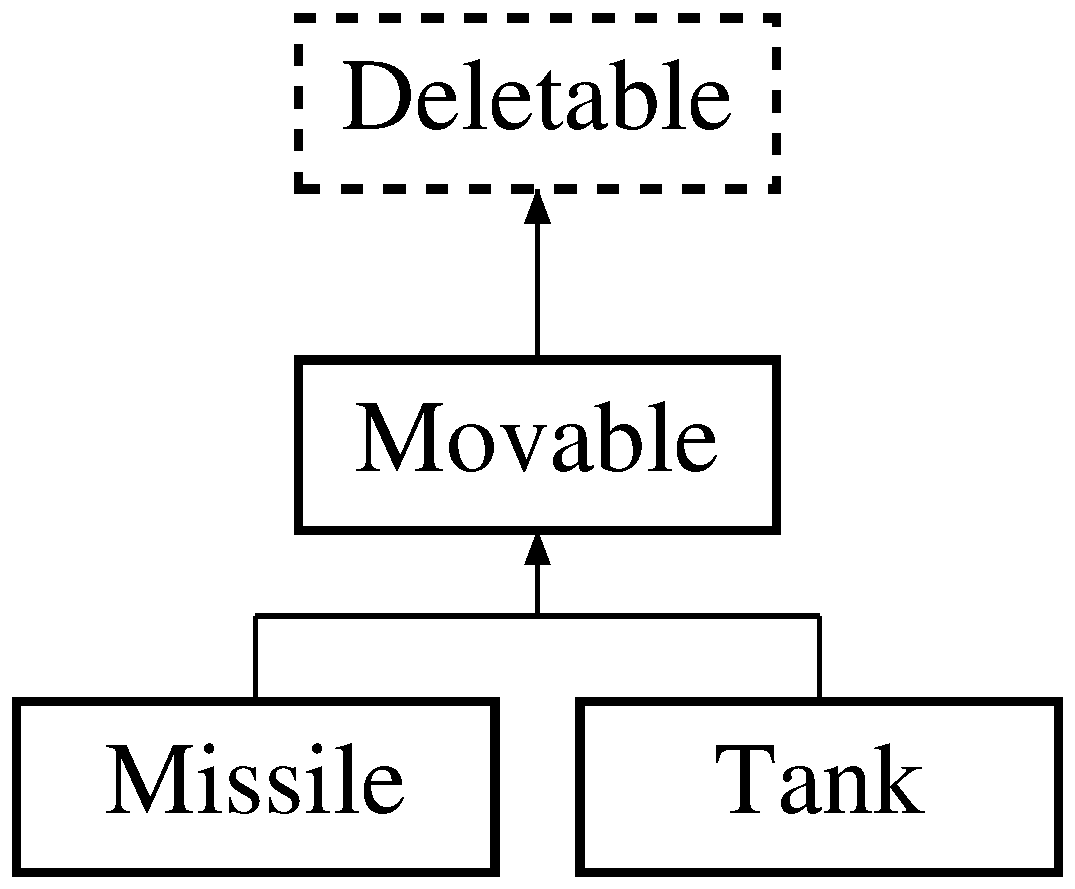
\includegraphics[height=3.000000cm]{classMovable}
\end{center}
\end{figure}
\subsection*{Public Member Functions}
\begin{DoxyCompactItemize}
\item 
\hyperlink{classMovable_a053cf48796f1aef5b6f6cb4c6b22db78}{Movable} ()
\begin{DoxyCompactList}\small\item\em Constructor. \end{DoxyCompactList}\item 
virtual void \hyperlink{classMovable_adefaf61339698c5efec597529bf89310}{move\-Forward} ()=0
\begin{DoxyCompactList}\small\item\em Move a moveable entity forward. \end{DoxyCompactList}\item 
virtual void \hyperlink{classMovable_a9c03e7ac263902159579d7f83e9b6dee}{move\-Backward} ()=0
\begin{DoxyCompactList}\small\item\em Move a moveable entity backward. \end{DoxyCompactList}\item 
virtual void \hyperlink{classMovable_a422b71ade02b9034600f51bc55d58c90}{rotate\-Left} ()=0
\begin{DoxyCompactList}\small\item\em Rotate a moveable entity left. \end{DoxyCompactList}\item 
virtual void \hyperlink{classMovable_a821480cb8ffd047b39a907c6cf07dd84}{rotate\-Right} ()=0
\begin{DoxyCompactList}\small\item\em Rotate a moveable entity right. \end{DoxyCompactList}\item 
virtual const \hyperlink{Structures_8h_a6fef29d9424addfa69bdd2a379424896}{blocked\-\_\-status} \hyperlink{classMovable_a40db320f27f5be1882553298677702c8}{is\-Blocked} ()=0
\begin{DoxyCompactList}\small\item\em Check state of entity to see number of times it has been blocked by another object. \end{DoxyCompactList}\item 
virtual void \hyperlink{classMovable_a0bb485f10776845305a683ed5e2ba1fc}{set\-Movement\-Direction} (const \hyperlink{Structures_8h_a0d0b88f27f3adf9452879b5d9f829026}{movement\-\_\-direction} Movement\-\_\-input)=0
\begin{DoxyCompactList}\small\item\em Set the movement direction of the entity. \end{DoxyCompactList}\item 
virtual \hyperlink{classMovable_ae629c22458180741deb4b67b9523c794}{$\sim$\-Movable} ()=0
\begin{DoxyCompactList}\small\item\em Destructor. \end{DoxyCompactList}\end{DoxyCompactItemize}
\subsection*{Static Protected Attributes}
\begin{DoxyCompactItemize}
\item 
static const int \hyperlink{classMovable_aff7e2a3e3d5a6059c4fe138aa47dc048}{\-\_\-missile\-Movement\-Speed} = 8
\begin{DoxyCompactList}\small\item\em Define the movement speed of a missile entity. \end{DoxyCompactList}\item 
static const int \hyperlink{classMovable_a54cb7d3465cc78ad7d8b2f7c2d842732}{\-\_\-tank\-Movement\-Speed} = 3
\begin{DoxyCompactList}\small\item\em Define the movement speed of a tank entity. \end{DoxyCompactList}\item 
static const int \hyperlink{classMovable_afde3611f73293d67497a39fed061e3a8}{\-\_\-missile\-Rotation\-Speed} = 45
\begin{DoxyCompactList}\small\item\em Define the rotation speed of a missile entity. \end{DoxyCompactList}\item 
static const int \hyperlink{classMovable_ab4ad35a0057bdbc80385c67bec5f1a60}{\-\_\-tank\-Rotation\-Speed} = 5
\begin{DoxyCompactList}\small\item\em Define the rotatioin speed of a tank entity. \end{DoxyCompactList}\end{DoxyCompactItemize}


\subsection{Detailed Description}
An Abstract-\/based class forming an interface for all Moveable objects within the game. 

This class is used as an interfacing template by all objects which are capable of moving. \hyperlink{classMovable}{Movable} classes are handled by the move manager who has access to all member functions within this class interface. 

Definition at line 20 of file Movable.\-h.



\subsection{Constructor \& Destructor Documentation}
\hypertarget{classMovable_a053cf48796f1aef5b6f6cb4c6b22db78}{\index{Movable@{Movable}!Movable@{Movable}}
\index{Movable@{Movable}!Movable@{Movable}}
\subsubsection[{Movable}]{\setlength{\rightskip}{0pt plus 5cm}Movable\-::\-Movable (
\begin{DoxyParamCaption}
{}
\end{DoxyParamCaption}
)}}\label{classMovable_a053cf48796f1aef5b6f6cb4c6b22db78}


Constructor. 



Definition at line 14 of file Movable.\-cpp.


\begin{DoxyCode}
15 \{
16 
17 \}
\end{DoxyCode}
\hypertarget{classMovable_ae629c22458180741deb4b67b9523c794}{\index{Movable@{Movable}!$\sim$\-Movable@{$\sim$\-Movable}}
\index{$\sim$\-Movable@{$\sim$\-Movable}!Movable@{Movable}}
\subsubsection[{$\sim$\-Movable}]{\setlength{\rightskip}{0pt plus 5cm}Movable\-::$\sim$\-Movable (
\begin{DoxyParamCaption}
{}
\end{DoxyParamCaption}
)\hspace{0.3cm}{\ttfamily [pure virtual]}}}\label{classMovable_ae629c22458180741deb4b67b9523c794}


Destructor. 



Definition at line 20 of file Movable.\-cpp.


\begin{DoxyCode}
21 \{
22 
23 \}
\end{DoxyCode}


\subsection{Member Function Documentation}
\hypertarget{classMovable_a40db320f27f5be1882553298677702c8}{\index{Movable@{Movable}!is\-Blocked@{is\-Blocked}}
\index{is\-Blocked@{is\-Blocked}!Movable@{Movable}}
\subsubsection[{is\-Blocked}]{\setlength{\rightskip}{0pt plus 5cm}virtual const {\bf blocked\-\_\-status} Movable\-::is\-Blocked (
\begin{DoxyParamCaption}
{}
\end{DoxyParamCaption}
)\hspace{0.3cm}{\ttfamily [pure virtual]}}}\label{classMovable_a40db320f27f5be1882553298677702c8}


Check state of entity to see number of times it has been blocked by another object. 



Implemented in \hyperlink{classTank_a6ca225d5f7a4c3b835da4a157b86c692}{Tank}, and \hyperlink{classMissile_a2c86874bf5e6bde8cb97f4ed1a07c3ea}{Missile}.

\hypertarget{classMovable_a9c03e7ac263902159579d7f83e9b6dee}{\index{Movable@{Movable}!move\-Backward@{move\-Backward}}
\index{move\-Backward@{move\-Backward}!Movable@{Movable}}
\subsubsection[{move\-Backward}]{\setlength{\rightskip}{0pt plus 5cm}virtual void Movable\-::move\-Backward (
\begin{DoxyParamCaption}
{}
\end{DoxyParamCaption}
)\hspace{0.3cm}{\ttfamily [pure virtual]}}}\label{classMovable_a9c03e7ac263902159579d7f83e9b6dee}


Move a moveable entity backward. 



Implemented in \hyperlink{classTank_a6fa5abbf02267f1e30e485b043abc1c2}{Tank}, and \hyperlink{classMissile_a8d8348b91961ff0c163d7d24bd9599a8}{Missile}.

\hypertarget{classMovable_adefaf61339698c5efec597529bf89310}{\index{Movable@{Movable}!move\-Forward@{move\-Forward}}
\index{move\-Forward@{move\-Forward}!Movable@{Movable}}
\subsubsection[{move\-Forward}]{\setlength{\rightskip}{0pt plus 5cm}virtual void Movable\-::move\-Forward (
\begin{DoxyParamCaption}
{}
\end{DoxyParamCaption}
)\hspace{0.3cm}{\ttfamily [pure virtual]}}}\label{classMovable_adefaf61339698c5efec597529bf89310}


Move a moveable entity forward. 



Implemented in \hyperlink{classTank_a7d4317a50c215c97679cf9d2fb40e223}{Tank}, and \hyperlink{classMissile_a4b6a45a5129b97a6e5383123dffab0c3}{Missile}.

\hypertarget{classMovable_a422b71ade02b9034600f51bc55d58c90}{\index{Movable@{Movable}!rotate\-Left@{rotate\-Left}}
\index{rotate\-Left@{rotate\-Left}!Movable@{Movable}}
\subsubsection[{rotate\-Left}]{\setlength{\rightskip}{0pt plus 5cm}virtual void Movable\-::rotate\-Left (
\begin{DoxyParamCaption}
{}
\end{DoxyParamCaption}
)\hspace{0.3cm}{\ttfamily [pure virtual]}}}\label{classMovable_a422b71ade02b9034600f51bc55d58c90}


Rotate a moveable entity left. 



Implemented in \hyperlink{classTank_aed009351545e9019140e75bd8365e1ad}{Tank}, and \hyperlink{classMissile_a1c7ed80bd656b0af5b3872f4225978e3}{Missile}.

\hypertarget{classMovable_a821480cb8ffd047b39a907c6cf07dd84}{\index{Movable@{Movable}!rotate\-Right@{rotate\-Right}}
\index{rotate\-Right@{rotate\-Right}!Movable@{Movable}}
\subsubsection[{rotate\-Right}]{\setlength{\rightskip}{0pt plus 5cm}virtual void Movable\-::rotate\-Right (
\begin{DoxyParamCaption}
{}
\end{DoxyParamCaption}
)\hspace{0.3cm}{\ttfamily [pure virtual]}}}\label{classMovable_a821480cb8ffd047b39a907c6cf07dd84}


Rotate a moveable entity right. 



Implemented in \hyperlink{classTank_a61c8d236aa98a258276654d02820966f}{Tank}, and \hyperlink{classMissile_aeccfdf94a02fa86545296f4c38857ef8}{Missile}.

\hypertarget{classMovable_a0bb485f10776845305a683ed5e2ba1fc}{\index{Movable@{Movable}!set\-Movement\-Direction@{set\-Movement\-Direction}}
\index{set\-Movement\-Direction@{set\-Movement\-Direction}!Movable@{Movable}}
\subsubsection[{set\-Movement\-Direction}]{\setlength{\rightskip}{0pt plus 5cm}virtual void Movable\-::set\-Movement\-Direction (
\begin{DoxyParamCaption}
\item[{const {\bf movement\-\_\-direction}}]{Movement\-\_\-input}
\end{DoxyParamCaption}
)\hspace{0.3cm}{\ttfamily [pure virtual]}}}\label{classMovable_a0bb485f10776845305a683ed5e2ba1fc}


Set the movement direction of the entity. 



Implemented in \hyperlink{classTank_ae283f9665d114b742cb521acbf0897fe}{Tank}, and \hyperlink{classMissile_a5bff45d0243e353acdf610fdade02bb0}{Missile}.



\subsection{Member Data Documentation}
\hypertarget{classMovable_aff7e2a3e3d5a6059c4fe138aa47dc048}{\index{Movable@{Movable}!\-\_\-missile\-Movement\-Speed@{\-\_\-missile\-Movement\-Speed}}
\index{\-\_\-missile\-Movement\-Speed@{\-\_\-missile\-Movement\-Speed}!Movable@{Movable}}
\subsubsection[{\-\_\-missile\-Movement\-Speed}]{\setlength{\rightskip}{0pt plus 5cm}const int Movable\-::\-\_\-missile\-Movement\-Speed = 8\hspace{0.3cm}{\ttfamily [static]}, {\ttfamily [protected]}}}\label{classMovable_aff7e2a3e3d5a6059c4fe138aa47dc048}


Define the movement speed of a missile entity. 



Definition at line 44 of file Movable.\-h.



Referenced by Missile\-::move\-Backward(), and Missile\-::move\-Forward().

\hypertarget{classMovable_afde3611f73293d67497a39fed061e3a8}{\index{Movable@{Movable}!\-\_\-missile\-Rotation\-Speed@{\-\_\-missile\-Rotation\-Speed}}
\index{\-\_\-missile\-Rotation\-Speed@{\-\_\-missile\-Rotation\-Speed}!Movable@{Movable}}
\subsubsection[{\-\_\-missile\-Rotation\-Speed}]{\setlength{\rightskip}{0pt plus 5cm}const int Movable\-::\-\_\-missile\-Rotation\-Speed = 45\hspace{0.3cm}{\ttfamily [static]}, {\ttfamily [protected]}}}\label{classMovable_afde3611f73293d67497a39fed061e3a8}


Define the rotation speed of a missile entity. 



Definition at line 48 of file Movable.\-h.

\hypertarget{classMovable_a54cb7d3465cc78ad7d8b2f7c2d842732}{\index{Movable@{Movable}!\-\_\-tank\-Movement\-Speed@{\-\_\-tank\-Movement\-Speed}}
\index{\-\_\-tank\-Movement\-Speed@{\-\_\-tank\-Movement\-Speed}!Movable@{Movable}}
\subsubsection[{\-\_\-tank\-Movement\-Speed}]{\setlength{\rightskip}{0pt plus 5cm}const int Movable\-::\-\_\-tank\-Movement\-Speed = 3\hspace{0.3cm}{\ttfamily [static]}, {\ttfamily [protected]}}}\label{classMovable_a54cb7d3465cc78ad7d8b2f7c2d842732}


Define the movement speed of a tank entity. 



Definition at line 46 of file Movable.\-h.



Referenced by Tank\-::move\-Backward(), and Tank\-::move\-Forward().

\hypertarget{classMovable_ab4ad35a0057bdbc80385c67bec5f1a60}{\index{Movable@{Movable}!\-\_\-tank\-Rotation\-Speed@{\-\_\-tank\-Rotation\-Speed}}
\index{\-\_\-tank\-Rotation\-Speed@{\-\_\-tank\-Rotation\-Speed}!Movable@{Movable}}
\subsubsection[{\-\_\-tank\-Rotation\-Speed}]{\setlength{\rightskip}{0pt plus 5cm}const int Movable\-::\-\_\-tank\-Rotation\-Speed = 5\hspace{0.3cm}{\ttfamily [static]}, {\ttfamily [protected]}}}\label{classMovable_ab4ad35a0057bdbc80385c67bec5f1a60}


Define the rotatioin speed of a tank entity. 



Definition at line 50 of file Movable.\-h.



Referenced by Tank\-::rotate\-Left(), and Tank\-::rotate\-Right().



The documentation for this class was generated from the following files\-:\begin{DoxyCompactItemize}
\item 
\hyperlink{Movable_8h}{Movable.\-h}\item 
\hyperlink{Movable_8cpp}{Movable.\-cpp}\end{DoxyCompactItemize}

\hypertarget{classMoveManager}{\section{Move\-Manager Class Reference}
\label{classMoveManager}\index{Move\-Manager@{Move\-Manager}}
}


{\ttfamily \#include $<$Move\-Manager.\-h$>$}

Inheritance diagram for Move\-Manager\-:\begin{figure}[H]
\begin{center}
\leavevmode
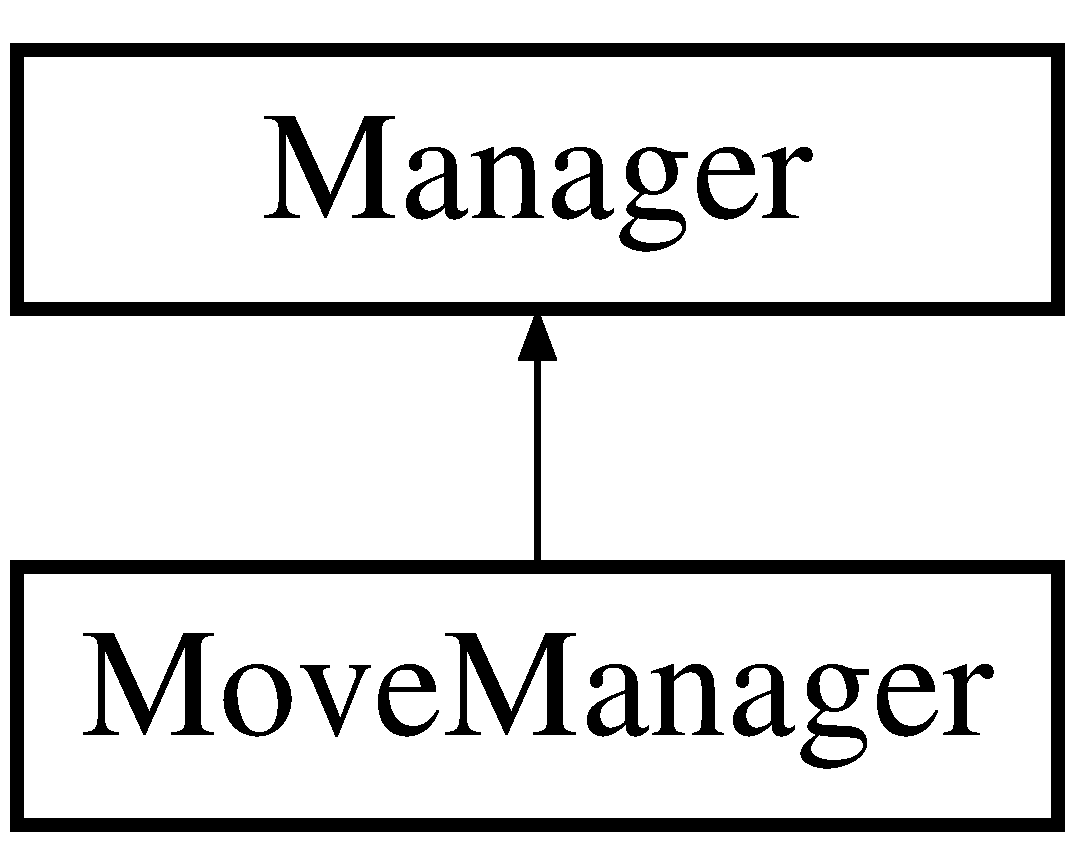
\includegraphics[height=2.000000cm]{classMoveManager}
\end{center}
\end{figure}
\subsection*{Public Member Functions}
\begin{DoxyCompactItemize}
\item 
\hyperlink{classMoveManager_a57ac62af15a2d9f9ed9b9ae96ea7900f}{Move\-Manager} ()
\begin{DoxyCompactList}\small\item\em Constructor. \end{DoxyCompactList}\item 
void \hyperlink{classMoveManager_a1e21cd4f542f801e84b57fd5f11f1154}{manage} (const \hyperlink{classActionData}{Action\-Data} \&action\-\_\-data\-\_\-container)
\begin{DoxyCompactList}\small\item\em Move all movable entities within the world. \end{DoxyCompactList}\item 
void \hyperlink{classMoveManager_a9f49f128a880d4f94c529c6aafab880e}{add\-New\-Entity} (std\-::weak\-\_\-ptr$<$ \hyperlink{classMovable}{Movable} $>$ new\-\_\-entity)
\begin{DoxyCompactList}\small\item\em Add Movable-\/type shared\-\_\-ptr's to the Move\-Managers internal data members. \end{DoxyCompactList}\item 
virtual \hyperlink{classMoveManager_a1de20c7414d1511c5b3a58196a557d94}{$\sim$\-Move\-Manager} ()
\begin{DoxyCompactList}\small\item\em Destructor for \hyperlink{classMoveManager}{Move\-Manager}. \end{DoxyCompactList}\end{DoxyCompactItemize}
\subsection*{Private Member Functions}
\begin{DoxyCompactItemize}
\item 
void \hyperlink{classMoveManager_a543e6c5900c59fc90ccef88a1317430a}{remove\-Garbage} ()
\begin{DoxyCompactList}\small\item\em Removes all deleted entities from move manager. \end{DoxyCompactList}\end{DoxyCompactItemize}
\subsection*{Private Attributes}
\begin{DoxyCompactItemize}
\item 
std\-::vector$<$ std\-::weak\-\_\-ptr\\*
$<$ \hyperlink{classMovable}{Movable} $>$ $>$ \hyperlink{classMoveManager_a7fc3d147dbcc1df9e2099e193bca489d}{\-\_\-movables}
\end{DoxyCompactItemize}


\subsection{Detailed Description}


Definition at line 21 of file Move\-Manager.\-h.



\subsection{Constructor \& Destructor Documentation}
\hypertarget{classMoveManager_a57ac62af15a2d9f9ed9b9ae96ea7900f}{\index{Move\-Manager@{Move\-Manager}!Move\-Manager@{Move\-Manager}}
\index{Move\-Manager@{Move\-Manager}!MoveManager@{Move\-Manager}}
\subsubsection[{Move\-Manager}]{\setlength{\rightskip}{0pt plus 5cm}Move\-Manager\-::\-Move\-Manager (
\begin{DoxyParamCaption}
{}
\end{DoxyParamCaption}
)}}\label{classMoveManager_a57ac62af15a2d9f9ed9b9ae96ea7900f}


Constructor. 

This constructor is minimal. Entities are associated to \hyperlink{classMoveManager}{Move\-Manager} through the add\-New\-Entities function 

Definition at line 18 of file Move\-Manager.\-cpp.


\begin{DoxyCode}
19 \{
20 
21 \}
\end{DoxyCode}
\hypertarget{classMoveManager_a1de20c7414d1511c5b3a58196a557d94}{\index{Move\-Manager@{Move\-Manager}!$\sim$\-Move\-Manager@{$\sim$\-Move\-Manager}}
\index{$\sim$\-Move\-Manager@{$\sim$\-Move\-Manager}!MoveManager@{Move\-Manager}}
\subsubsection[{$\sim$\-Move\-Manager}]{\setlength{\rightskip}{0pt plus 5cm}Move\-Manager\-::$\sim$\-Move\-Manager (
\begin{DoxyParamCaption}
{}
\end{DoxyParamCaption}
)\hspace{0.3cm}{\ttfamily [virtual]}}}\label{classMoveManager_a1de20c7414d1511c5b3a58196a557d94}


Destructor for \hyperlink{classMoveManager}{Move\-Manager}. 

Destructor.

No further implementation defined 

Definition at line 26 of file Move\-Manager.\-cpp.


\begin{DoxyCode}
27 \{
28 
29 \}
\end{DoxyCode}


\subsection{Member Function Documentation}
\hypertarget{classMoveManager_a9f49f128a880d4f94c529c6aafab880e}{\index{Move\-Manager@{Move\-Manager}!add\-New\-Entity@{add\-New\-Entity}}
\index{add\-New\-Entity@{add\-New\-Entity}!MoveManager@{Move\-Manager}}
\subsubsection[{add\-New\-Entity}]{\setlength{\rightskip}{0pt plus 5cm}void Move\-Manager\-::add\-New\-Entity (
\begin{DoxyParamCaption}
\item[{std\-::weak\-\_\-ptr$<$ {\bf Movable} $>$}]{new\-\_\-entity}
\end{DoxyParamCaption}
)}}\label{classMoveManager_a9f49f128a880d4f94c529c6aafab880e}


Add Movable-\/type shared\-\_\-ptr's to the Move\-Managers internal data members. 

Used to add new weak pointer instances to the \hyperlink{classMoveManager}{Move\-Manager} private vector.

This function allows for new entities to be passed and managed by the Movement\-Manager by adding the weak pointers of created \hyperlink{classMovable}{Movable} objects to the classes private vector. 

Definition at line 229 of file Move\-Manager.\-cpp.



References \-\_\-movables.



Referenced by Game\-::add\-Movable(), main(), and T\-E\-S\-T().


\begin{DoxyCode}
230 \{
231     \hyperlink{classMoveManager_a7fc3d147dbcc1df9e2099e193bca489d}{\_movables}.push\_back(new\_entity);
232 \}
\end{DoxyCode}
\hypertarget{classMoveManager_a1e21cd4f542f801e84b57fd5f11f1154}{\index{Move\-Manager@{Move\-Manager}!manage@{manage}}
\index{manage@{manage}!MoveManager@{Move\-Manager}}
\subsubsection[{manage}]{\setlength{\rightskip}{0pt plus 5cm}void Move\-Manager\-::manage (
\begin{DoxyParamCaption}
\item[{const {\bf Action\-Data} \&}]{action\-\_\-data\-\_\-container}
\end{DoxyParamCaption}
)}}\label{classMoveManager_a1e21cd4f542f801e84b57fd5f11f1154}


Move all movable entities within the world. 

The \hyperlink{classMoveManager}{Move\-Manager} Logical Management function.

The function works by evaluating the private vector of weak\-\_\-pointers stored within \hyperlink{classMoveManager}{Move\-Manager} and determining if each one can move or not. A 'blocked' status wil result in an object not being able to move (or it will be reflected in the case of a missile) 
\begin{DoxyParams}{Parameters}
{\em action\-\_\-data\-\_\-contatiner} & \-:\-: a data container with all relevant move info for the current management cycle. \\
\hline
\end{DoxyParams}


Definition at line 38 of file Move\-Manager.\-cpp.



References \-\_\-movables, blocked\-\_\-horizontally, blocked\-\_\-vertically, actions\-\_\-info\-::change\-\_\-1, actions\-\_\-info\-::change\-\_\-2, do\-\_\-nothing, forward, Action\-Data\-::give\-Action\-Info(), actions\-\_\-info\-::move\-\_\-1, actions\-\_\-info\-::move\-\_\-2, move\-Backward, move\-Forward, p1\-\_\-missile, p1\-\_\-tank, p2\-\_\-missile, p2\-\_\-tank, remove\-Garbage(), reverse, rotate\-\_\-left, rotate\-\_\-right, rotate\-Left, rotate\-Right, turret\-\_\-missile, and unblocked.



Referenced by main(), Game\-::run\-All\-Managers(), and T\-E\-S\-T().


\begin{DoxyCode}
39 \{
40     \hyperlink{structactions__info}{actions\_info} managerInstructions = action\_data\_container.
      \hyperlink{classActionData_ab2f5b210968c91a01ed1439904b3ffee}{giveActionInfo}();
41 
42     \textcolor{comment}{//Remove any "corpses" found within the movable vector}
43     \hyperlink{classMoveManager_a543e6c5900c59fc90ccef88a1317430a}{removeGarbage}();
44 
45 
46     \textcolor{keyword}{auto} moveables\_iterator = \hyperlink{classMoveManager_a7fc3d147dbcc1df9e2099e193bca489d}{\_movables}.begin();
47     \textcolor{keywordflow}{for}(; moveables\_iterator != \hyperlink{classMoveManager_a7fc3d147dbcc1df9e2099e193bca489d}{\_movables}.end(); moveables\_iterator++)
48     \{
49         \textcolor{comment}{//Convert iterator to Weak pointer}
50         std::weak\_ptr<Movable> entity\_mov\_wp = (*moveables\_iterator);
51 
52         \textcolor{comment}{//Lock as Shared Pointer}
53         std::shared\_ptr<Movable> entity\_mov\_sp = entity\_mov\_wp.lock();
54 
55         \textcolor{comment}{//Make changes to player 1's tank if movement has been captured}
56         \textcolor{keywordflow}{if} ((managerInstructions.\hyperlink{structactions__info_a69ac673533838f973f09492a12516816}{change\_1} == \textcolor{keyword}{true}) && (entity\_mov\_sp->getType() == 
      \hyperlink{Structures_8h_a6d8f83e710b27d4f86c45f0bb77066e3a31fa78b2b7dd774f5158a16ef230932e}{p1\_tank}))
57         \{
58             \textcolor{keywordflow}{if}(entity\_mov\_sp->isBlocked() == \hyperlink{Structures_8h_a6fef29d9424addfa69bdd2a379424896a1596fbf6035468467c790068b609ced3}{unblocked})
59             \{
60                 \textcolor{keywordflow}{switch}(managerInstructions.\hyperlink{structactions__info_a5cb853144009b2bfb7e58c7bf43e2a42}{move\_1})
61                 \{
62                     \textcolor{keywordflow}{case} \hyperlink{Structures_8h_abf3d9daa4559fb2f9e16fc1836fead1ba726a0af5164861adac8c015a742dcf21}{forward}:
63                         entity\_mov\_sp->moveForward();
64                         entity\_mov\_sp->setMovementDirection(\hyperlink{Structures_8h_a0d0b88f27f3adf9452879b5d9f829026a4c3e911cdfbc22463cb4e96bd7a50327}{moveForward});
65                         \textcolor{keywordflow}{break};
66 
67                     \textcolor{keywordflow}{case} \hyperlink{Structures_8h_abf3d9daa4559fb2f9e16fc1836fead1ba5a40f8ecbed801e00fddb306fc5666f0}{reverse}:
68                         entity\_mov\_sp->moveBackward();
69                         entity\_mov\_sp->setMovementDirection(\hyperlink{Structures_8h_a0d0b88f27f3adf9452879b5d9f829026ac32aa98894056eae24f1c8f7af930584}{moveBackward});
70                         \textcolor{keywordflow}{break};
71 
72                     \textcolor{keywordflow}{case} \hyperlink{Structures_8h_abf3d9daa4559fb2f9e16fc1836fead1ba980501baf8209a1bfe04fa435e2cbd3e}{rotate\_left}:
73                         entity\_mov\_sp->rotateLeft();
74                         entity\_mov\_sp->setMovementDirection(\hyperlink{Structures_8h_a0d0b88f27f3adf9452879b5d9f829026af8f913ac2071c34908f89a0170ff0425}{rotateLeft});
75                         \textcolor{keywordflow}{break};
76 
77                     \textcolor{keywordflow}{case} \hyperlink{Structures_8h_abf3d9daa4559fb2f9e16fc1836fead1bae58291f8d743551c95d70a7129b4c544}{rotate\_right}:
78                         entity\_mov\_sp->rotateRight();
79                         entity\_mov\_sp->setMovementDirection(\hyperlink{Structures_8h_a0d0b88f27f3adf9452879b5d9f829026a3b81355949ce720f9c0318b01aaf76ee}{rotateRight});
80                         \textcolor{keywordflow}{break};
81 
82                     \textcolor{keywordflow}{case} \hyperlink{Structures_8h_abf3d9daa4559fb2f9e16fc1836fead1ba562e0b8966ea62e894cd91a30eccfc8a}{do\_nothing}:
83                         \textcolor{keywordflow}{break};
84                 \}
85             \}
86             \textcolor{keywordflow}{else} \textcolor{comment}{//if the object is blocked}
87             \{
88                 \textcolor{keywordflow}{switch}(managerInstructions.\hyperlink{structactions__info_a5cb853144009b2bfb7e58c7bf43e2a42}{move\_1})
89                 \{
90                     \textcolor{keywordflow}{case} \hyperlink{Structures_8h_abf3d9daa4559fb2f9e16fc1836fead1ba726a0af5164861adac8c015a742dcf21}{forward}:
91                         entity\_mov\_sp->setMovementDirection(\hyperlink{Structures_8h_a0d0b88f27f3adf9452879b5d9f829026a4c3e911cdfbc22463cb4e96bd7a50327}{moveForward});
92                     \textcolor{keywordflow}{break};
93 
94                     \textcolor{keywordflow}{case} \hyperlink{Structures_8h_abf3d9daa4559fb2f9e16fc1836fead1ba5a40f8ecbed801e00fddb306fc5666f0}{reverse}:
95                         entity\_mov\_sp->setMovementDirection(\hyperlink{Structures_8h_a0d0b88f27f3adf9452879b5d9f829026ac32aa98894056eae24f1c8f7af930584}{moveBackward});
96                         \textcolor{keywordflow}{break};
97 
98                     \textcolor{keywordflow}{case} \hyperlink{Structures_8h_abf3d9daa4559fb2f9e16fc1836fead1ba980501baf8209a1bfe04fa435e2cbd3e}{rotate\_left}:
99                         entity\_mov\_sp->setMovementDirection(\hyperlink{Structures_8h_a0d0b88f27f3adf9452879b5d9f829026af8f913ac2071c34908f89a0170ff0425}{rotateLeft});
100                         \textcolor{keywordflow}{break};
101 
102                     \textcolor{keywordflow}{case} \hyperlink{Structures_8h_abf3d9daa4559fb2f9e16fc1836fead1bae58291f8d743551c95d70a7129b4c544}{rotate\_right}:
103                         entity\_mov\_sp->setMovementDirection(\hyperlink{Structures_8h_a0d0b88f27f3adf9452879b5d9f829026a3b81355949ce720f9c0318b01aaf76ee}{rotateRight});
104                     \textcolor{keywordflow}{case} \hyperlink{Structures_8h_abf3d9daa4559fb2f9e16fc1836fead1ba562e0b8966ea62e894cd91a30eccfc8a}{do\_nothing}:
105                         \textcolor{keywordflow}{break};
106                 \}
107             \}
108         \} \textcolor{comment}{// If for P1 tank}
109 
110          \textcolor{comment}{//Make changes to player 2's tank if movement has been captured}
111         \textcolor{keywordflow}{if} ((managerInstructions.\hyperlink{structactions__info_a0f20d9c244d92a71dad9cf8ce10cd2f2}{change\_2} == \textcolor{keyword}{true}) && (entity\_mov\_sp->getType() == 
      \hyperlink{Structures_8h_a6d8f83e710b27d4f86c45f0bb77066e3a3d48d62c7b88e7ee171698fe56dc9e59}{p2\_tank}))
112         \{
113             \textcolor{keywordflow}{if}(entity\_mov\_sp->isBlocked() == \hyperlink{Structures_8h_a6fef29d9424addfa69bdd2a379424896a1596fbf6035468467c790068b609ced3}{unblocked})
114             \{
115                 \textcolor{keywordflow}{switch}(managerInstructions.\hyperlink{structactions__info_adf9ed4a9ad4b604295846d06872e0ebf}{move\_2})
116                 \{
117                   \textcolor{keywordflow}{case} \hyperlink{Structures_8h_abf3d9daa4559fb2f9e16fc1836fead1ba726a0af5164861adac8c015a742dcf21}{forward}:
118                         entity\_mov\_sp->moveForward();
119                         entity\_mov\_sp->setMovementDirection(\hyperlink{Structures_8h_a0d0b88f27f3adf9452879b5d9f829026a4c3e911cdfbc22463cb4e96bd7a50327}{moveForward});
120                         \textcolor{keywordflow}{break};
121 
122                     \textcolor{keywordflow}{case} \hyperlink{Structures_8h_abf3d9daa4559fb2f9e16fc1836fead1ba5a40f8ecbed801e00fddb306fc5666f0}{reverse}:
123                         entity\_mov\_sp->moveBackward();
124                         entity\_mov\_sp->setMovementDirection(\hyperlink{Structures_8h_a0d0b88f27f3adf9452879b5d9f829026ac32aa98894056eae24f1c8f7af930584}{moveBackward});
125                         \textcolor{keywordflow}{break};
126 
127                     \textcolor{keywordflow}{case} \hyperlink{Structures_8h_abf3d9daa4559fb2f9e16fc1836fead1ba980501baf8209a1bfe04fa435e2cbd3e}{rotate\_left}:
128                         entity\_mov\_sp->rotateLeft();
129                         entity\_mov\_sp->setMovementDirection(\hyperlink{Structures_8h_a0d0b88f27f3adf9452879b5d9f829026af8f913ac2071c34908f89a0170ff0425}{rotateLeft});
130                         \textcolor{keywordflow}{break};
131 
132                     \textcolor{keywordflow}{case} \hyperlink{Structures_8h_abf3d9daa4559fb2f9e16fc1836fead1bae58291f8d743551c95d70a7129b4c544}{rotate\_right}:
133                         entity\_mov\_sp->rotateRight();
134                         entity\_mov\_sp->setMovementDirection(\hyperlink{Structures_8h_a0d0b88f27f3adf9452879b5d9f829026a3b81355949ce720f9c0318b01aaf76ee}{rotateRight});
135                         \textcolor{keywordflow}{break};
136 
137                     \textcolor{keywordflow}{case} \hyperlink{Structures_8h_abf3d9daa4559fb2f9e16fc1836fead1ba562e0b8966ea62e894cd91a30eccfc8a}{do\_nothing}:
138                         \textcolor{keywordflow}{break};
139                 \}
140             \}
141             \textcolor{keywordflow}{else} \textcolor{comment}{//if the object is blocked}
142             \{
143                 \textcolor{keywordflow}{switch}(managerInstructions.\hyperlink{structactions__info_adf9ed4a9ad4b604295846d06872e0ebf}{move\_2})
144                 \{
145                    \textcolor{keywordflow}{case} \hyperlink{Structures_8h_abf3d9daa4559fb2f9e16fc1836fead1ba726a0af5164861adac8c015a742dcf21}{forward}:
146                         entity\_mov\_sp->setMovementDirection(\hyperlink{Structures_8h_a0d0b88f27f3adf9452879b5d9f829026a4c3e911cdfbc22463cb4e96bd7a50327}{moveForward});
147                     \textcolor{keywordflow}{break};
148 
149                     \textcolor{keywordflow}{case} \hyperlink{Structures_8h_abf3d9daa4559fb2f9e16fc1836fead1ba5a40f8ecbed801e00fddb306fc5666f0}{reverse}:
150                         entity\_mov\_sp->setMovementDirection(\hyperlink{Structures_8h_a0d0b88f27f3adf9452879b5d9f829026ac32aa98894056eae24f1c8f7af930584}{moveBackward});
151                         \textcolor{keywordflow}{break};
152 
153                     \textcolor{keywordflow}{case} \hyperlink{Structures_8h_abf3d9daa4559fb2f9e16fc1836fead1ba980501baf8209a1bfe04fa435e2cbd3e}{rotate\_left}:
154                         entity\_mov\_sp->setMovementDirection(\hyperlink{Structures_8h_a0d0b88f27f3adf9452879b5d9f829026af8f913ac2071c34908f89a0170ff0425}{rotateLeft});
155                         \textcolor{keywordflow}{break};
156 
157                     \textcolor{keywordflow}{case} \hyperlink{Structures_8h_abf3d9daa4559fb2f9e16fc1836fead1bae58291f8d743551c95d70a7129b4c544}{rotate\_right}:
158                         entity\_mov\_sp->setMovementDirection(\hyperlink{Structures_8h_a0d0b88f27f3adf9452879b5d9f829026a3b81355949ce720f9c0318b01aaf76ee}{rotateRight});
159                     \textcolor{keywordflow}{case} \hyperlink{Structures_8h_abf3d9daa4559fb2f9e16fc1836fead1ba562e0b8966ea62e894cd91a30eccfc8a}{do\_nothing}:
160                         \textcolor{keywordflow}{break};
161                 \}
162             \}
163         \}
164 
165         \textcolor{comment}{//Missiles will always move along their trajectory each management cycle}
166         \textcolor{comment}{//Exception if a missile hits a barrier}
167 
168         \textcolor{comment}{//Missile has hit a barrier}
169         \textcolor{keywordflow}{if} (((entity\_mov\_sp->getType() == \hyperlink{Structures_8h_a6d8f83e710b27d4f86c45f0bb77066e3af89bc631e9b0140ed004b5ce2db5330c}{p1\_missile}) ||
170             (entity\_mov\_sp->getType() == \hyperlink{Structures_8h_a6d8f83e710b27d4f86c45f0bb77066e3a47100170e5852d632dfe65582a18256d}{p2\_missile}) ||
171             (entity\_mov\_sp->getType() == \hyperlink{Structures_8h_a6d8f83e710b27d4f86c45f0bb77066e3a8f552a1e495ced5aa8775faa1b6a757b}{turret\_missile}))
172              && (entity\_mov\_sp->isBlocked() == \hyperlink{Structures_8h_a6fef29d9424addfa69bdd2a379424896a582e6420c60bcec29729790197d0459f}{blocked\_horizontally}))
173         \{
174             entity\_mov\_sp->rotateLeft();
175             entity\_mov\_sp->moveForward();
176         \}
177 
178          \textcolor{keywordflow}{if} (((entity\_mov\_sp->getType() == \hyperlink{Structures_8h_a6d8f83e710b27d4f86c45f0bb77066e3af89bc631e9b0140ed004b5ce2db5330c}{p1\_missile}) ||
179             (entity\_mov\_sp->getType() == \hyperlink{Structures_8h_a6d8f83e710b27d4f86c45f0bb77066e3a47100170e5852d632dfe65582a18256d}{p2\_missile}) ||
180             (entity\_mov\_sp->getType() == \hyperlink{Structures_8h_a6d8f83e710b27d4f86c45f0bb77066e3a8f552a1e495ced5aa8775faa1b6a757b}{turret\_missile}))
181              && (entity\_mov\_sp->isBlocked() == \hyperlink{Structures_8h_a6fef29d9424addfa69bdd2a379424896a5b5e63da31bc787008b9f40686347e45}{blocked\_vertically}))
182         \{
183             entity\_mov\_sp->rotateRight();
184             entity\_mov\_sp->moveForward();
185         \}
186         \textcolor{comment}{//Missile moves forward}
187         \textcolor{keywordflow}{else} \textcolor{keywordflow}{if} (((entity\_mov\_sp->getType() == \hyperlink{Structures_8h_a6d8f83e710b27d4f86c45f0bb77066e3af89bc631e9b0140ed004b5ce2db5330c}{p1\_missile}) ||
188                  (entity\_mov\_sp->getType() == \hyperlink{Structures_8h_a6d8f83e710b27d4f86c45f0bb77066e3a47100170e5852d632dfe65582a18256d}{p2\_missile}) ||
189                  (entity\_mov\_sp->getType() == \hyperlink{Structures_8h_a6d8f83e710b27d4f86c45f0bb77066e3a8f552a1e495ced5aa8775faa1b6a757b}{turret\_missile}))
190                  && (entity\_mov\_sp->isBlocked() == \hyperlink{Structures_8h_a6fef29d9424addfa69bdd2a379424896a1596fbf6035468467c790068b609ced3}{unblocked}))
191         \{
192             entity\_mov\_sp->moveForward();
193         \}
194 
195     \}\textcolor{comment}{//Range-based for}
196 \}\textcolor{comment}{//Function}
\end{DoxyCode}
\hypertarget{classMoveManager_a543e6c5900c59fc90ccef88a1317430a}{\index{Move\-Manager@{Move\-Manager}!remove\-Garbage@{remove\-Garbage}}
\index{remove\-Garbage@{remove\-Garbage}!MoveManager@{Move\-Manager}}
\subsubsection[{remove\-Garbage}]{\setlength{\rightskip}{0pt plus 5cm}void Move\-Manager\-::remove\-Garbage (
\begin{DoxyParamCaption}
{}
\end{DoxyParamCaption}
)\hspace{0.3cm}{\ttfamily [private]}}}\label{classMoveManager_a543e6c5900c59fc90ccef88a1317430a}


Removes all deleted entities from move manager. 

This function uses the Move\-Managers vector of weak pointers which are asked to lock to determine whether or not they still point to an existing object. It the object does not exist, it is erased from the \hyperlink{classMoveManager}{Move\-Manager} vector 

Definition at line 204 of file Move\-Manager.\-cpp.



References \-\_\-movables.



Referenced by manage().


\begin{DoxyCode}
205 \{
206     \textcolor{keyword}{auto} removable = \hyperlink{classMoveManager_a7fc3d147dbcc1df9e2099e193bca489d}{\_movables}.begin();
207     \textcolor{keywordflow}{for} (; removable != \hyperlink{classMoveManager_a7fc3d147dbcc1df9e2099e193bca489d}{\_movables}.end();)
208     \{
209         \textcolor{comment}{//Convert iterator to Weak pointer}
210         std::weak\_ptr<Movable> removable\_wp = (*removable);
211         \textcolor{comment}{//Lock as Shared Pointer}
212         std::shared\_ptr<Movable> removable\_sp = removable\_wp.lock();
213         \textcolor{comment}{//Test to see if the shared pointer exists}
214         \textcolor{keywordflow}{if} (removable\_sp)
215         \{
216             removable++;
217         \}
218         \textcolor{keywordflow}{else}
219         \{
220             \hyperlink{classMoveManager_a7fc3d147dbcc1df9e2099e193bca489d}{\_movables}.erase(removable);
221         \}
222     \}
223 \}
\end{DoxyCode}


\subsection{Member Data Documentation}
\hypertarget{classMoveManager_a7fc3d147dbcc1df9e2099e193bca489d}{\index{Move\-Manager@{Move\-Manager}!\-\_\-movables@{\-\_\-movables}}
\index{\-\_\-movables@{\-\_\-movables}!MoveManager@{Move\-Manager}}
\subsubsection[{\-\_\-movables}]{\setlength{\rightskip}{0pt plus 5cm}std\-::vector$<$std\-::weak\-\_\-ptr$<${\bf Movable}$>$ $>$ Move\-Manager\-::\-\_\-movables\hspace{0.3cm}{\ttfamily [private]}}}\label{classMoveManager_a7fc3d147dbcc1df9e2099e193bca489d}


Definition at line 38 of file Move\-Manager.\-h.



Referenced by add\-New\-Entity(), manage(), and remove\-Garbage().



The documentation for this class was generated from the following files\-:\begin{DoxyCompactItemize}
\item 
\hyperlink{MoveManager_8h}{Move\-Manager.\-h}\item 
\hyperlink{MoveManager_8cpp}{Move\-Manager.\-cpp}\end{DoxyCompactItemize}

\hypertarget{classOrientation}{\section{Orientation Class Reference}
\label{classOrientation}\index{Orientation@{Orientation}}
}


{\ttfamily \#include $<$Orientation.\-h$>$}

\subsection*{Public Member Functions}
\begin{DoxyCompactItemize}
\item 
\hyperlink{classOrientation_ae2df457b68375ea4915f7fa1c161b116}{Orientation} (float origin\-\_\-x, float origin\-\_\-y, float width, float height, float rotation, bool controllable)
\begin{DoxyCompactList}\small\item\em Constructor that initialises all data members of the class. \end{DoxyCompactList}\item 
const float \hyperlink{classOrientation_a4d6b853f2ac00965d29e5bc36b94c949}{get\-Origin\-X} ()
\begin{DoxyCompactList}\small\item\em Returns the entity origin x value. \end{DoxyCompactList}\item 
const float \hyperlink{classOrientation_ae60c88b0525d6e536a1a068d3a99f74c}{get\-Origin\-Y} ()
\begin{DoxyCompactList}\small\item\em Returns the entity origin y value. \end{DoxyCompactList}\item 
const float \hyperlink{classOrientation_adf3e031c3ce102233782e6fdeb976ef3}{get\-Width} ()
\begin{DoxyCompactList}\small\item\em Returns the entity width. \end{DoxyCompactList}\item 
const float \hyperlink{classOrientation_af7c9a2f7547c76ce2408ac6fefacf9e1}{get\-Height} ()
\begin{DoxyCompactList}\small\item\em Returns the entity height. \end{DoxyCompactList}\item 
const float \hyperlink{classOrientation_ab3568e037a7dc7799d557f2bc6a3cf7d}{get\-Rotation} ()
\begin{DoxyCompactList}\small\item\em Returns the entity rotation. \end{DoxyCompactList}\item 
void \hyperlink{classOrientation_a1b5cd490e5bbbe2b8d683be389dbcbbe}{set\-Width} (const float width)
\begin{DoxyCompactList}\small\item\em Set the Width Value. \end{DoxyCompactList}\item 
void \hyperlink{classOrientation_a1adca89bc32128e2ca1cb937357f5006}{set\-Height} (const float height)
\begin{DoxyCompactList}\small\item\em Set the Height Value. \end{DoxyCompactList}\item 
void \hyperlink{classOrientation_ae1c8122591724b1b3bfcb0026b76e809}{move} (float movement\-\_\-in\-\_\-x, float movement\-\_\-in\-\_\-y)
\begin{DoxyCompactList}\small\item\em Move the entity by a distance. \end{DoxyCompactList}\item 
void \hyperlink{classOrientation_aa9e115b7f4ab487e3af532592416b247}{rotate} (float angle)
\begin{DoxyCompactList}\small\item\em Rotate the entity by a supplied angle. \end{DoxyCompactList}\item 
void \hyperlink{classOrientation_a478512ba497cd75f11be3aa3177cca6a}{set\-Move\-Direction} (const \hyperlink{Structures_8h_a0d0b88f27f3adf9452879b5d9f829026}{movement\-\_\-direction})
\begin{DoxyCompactList}\small\item\em Used to set the state of future collision detection. \end{DoxyCompactList}\item 
\hyperlink{structrect__corners}{rect\-\_\-corners} \& \hyperlink{classOrientation_a950dfe84e548582d8c3c573b5ff5fe42}{get\-Global\-Bounds} ()
\begin{DoxyCompactList}\small\item\em Retrieve Rectangular co-\/ordinates for collision detection. \end{DoxyCompactList}\item 
const \hyperlink{structrect__corners}{rect\-\_\-corners} \& \hyperlink{classOrientation_a5cc606289f774c8561af98d183586199}{get\-Aligned\-Global\-Bounds} ()
\begin{DoxyCompactList}\small\item\em Retrieve Rectangular co-\/ordinated for collision detection (Non-\/rotated) \end{DoxyCompactList}\item 
virtual \hyperlink{classOrientation_a8c96df6f0b3b9a9edc7f9a0a9cc10741}{$\sim$\-Orientation} ()
\begin{DoxyCompactList}\small\item\em Destructor. \end{DoxyCompactList}\item 
bool \hyperlink{classOrientation_a0195b81c78baadd074301bc019d11db8}{operator==} (\hyperlink{classOrientation}{Orientation} \&rhs) const 
\begin{DoxyCompactList}\small\item\em Equality operator overload for testing. \end{DoxyCompactList}\end{DoxyCompactItemize}
\subsection*{Private Member Functions}
\begin{DoxyCompactItemize}
\item 
void \hyperlink{classOrientation_aa1a923fcae4e94c8bbd319b094732d43}{set\-Global\-Bounds} ()
\begin{DoxyCompactList}\small\item\em Function used to calculate the non-\/axis-\/aligned (Complex) bounding box of the orientation entity. \end{DoxyCompactList}\item 
float \hyperlink{classOrientation_aadef2c8638c11919def962831d10934c}{get\-Relative\-X} () const 
\begin{DoxyCompactList}\small\item\em Used to determine the relative/future position of an orientation object. \end{DoxyCompactList}\item 
float \hyperlink{classOrientation_a9230d58e08959c61a26876769e9b6df0}{get\-Relative\-Y} () const 
\begin{DoxyCompactList}\small\item\em Used to determine the relative/future position of an orientation object. \end{DoxyCompactList}\item 
float \hyperlink{classOrientation_a3909302fb7aea90a0bc706871f0a072f}{get\-Relative\-Rotation} () const 
\begin{DoxyCompactList}\small\item\em Used to determine the relative/future rotation of an orientation object. \end{DoxyCompactList}\end{DoxyCompactItemize}
\subsection*{Private Attributes}
\begin{DoxyCompactItemize}
\item 
float \hyperlink{classOrientation_ae7ee03cf18222bb76433d577936d610e}{\-\_\-origin\-\_\-x}
\item 
float \hyperlink{classOrientation_affb8b0093da380404f865772bf52b3eb}{\-\_\-origin\-\_\-y}
\item 
float \hyperlink{classOrientation_a5052b45396fc5e6abcf343c60e1fa59d}{\-\_\-width}
\item 
float \hyperlink{classOrientation_adf3f5a166d15ee16f99612bc5c6ef080}{\-\_\-height}
\item 
float \hyperlink{classOrientation_ab75afc35c00f204c390ab2ffe716374a}{\-\_\-rotation}
\item 
\hyperlink{structrect__corners}{rect\-\_\-corners} \hyperlink{classOrientation_a92030f5994ff171542a5b6e5b104f2f1}{\-\_\-collison\-\_\-box}
\item 
bool \hyperlink{classOrientation_ab8577b28d6c1e445d55d113640f1ed07}{\-\_\-controllable}
\item 
\hyperlink{Structures_8h_a0d0b88f27f3adf9452879b5d9f829026}{movement\-\_\-direction} \hyperlink{classOrientation_a548b6090029335848c21f40f87811df9}{\-\_\-movement\-\_\-direction}
\end{DoxyCompactItemize}


\subsection{Detailed Description}


Definition at line 20 of file Orientation.\-h.



\subsection{Constructor \& Destructor Documentation}
\hypertarget{classOrientation_ae2df457b68375ea4915f7fa1c161b116}{\index{Orientation@{Orientation}!Orientation@{Orientation}}
\index{Orientation@{Orientation}!Orientation@{Orientation}}
\subsubsection[{Orientation}]{\setlength{\rightskip}{0pt plus 5cm}Orientation\-::\-Orientation (
\begin{DoxyParamCaption}
\item[{float}]{origin\-\_\-x, }
\item[{float}]{origin\-\_\-y, }
\item[{float}]{width, }
\item[{float}]{height, }
\item[{float}]{rotation, }
\item[{bool}]{controllable}
\end{DoxyParamCaption}
)}}\label{classOrientation_ae2df457b68375ea4915f7fa1c161b116}


Constructor that initialises all data members of the class. 

Constructor for \hyperlink{classOrientation}{Orientation} class.

Default constructor for the \hyperlink{classOrientation}{Orientation} class 
\begin{DoxyParams}{Parameters}
{\em origin\-\_\-x} & \-:\-: The initial x-\/coordinate of the orientation object \\
\hline
{\em origin\-\_\-y} & \-:\-: The initial y-\/coordinate of the orientation object \\
\hline
{\em width} & \-:\-: The sprite width which the orientation object will mimic \\
\hline
{\em height} & \-:\-: The sprite height which the orientation object will mimic \\
\hline
{\em rotation} & \-:\-: The initial rotation held by the orientation object \\
\hline
{\em controllable} & \-:\-: This destinguishes what type of bounding box the orientation class should create \\
\hline
\end{DoxyParams}


Definition at line 25 of file Orientation.\-cpp.



References \-\_\-movement\-\_\-direction, Move, and set\-Global\-Bounds().


\begin{DoxyCode}
25                                                                                                            
               :
26     \hyperlink{classOrientation_ae7ee03cf18222bb76433d577936d610e}{\_origin\_x}(origin\_x),
27     \hyperlink{classOrientation_affb8b0093da380404f865772bf52b3eb}{\_origin\_y}(origin\_y),
28     \hyperlink{classOrientation_a5052b45396fc5e6abcf343c60e1fa59d}{\_width}(width),
29     \hyperlink{classOrientation_adf3f5a166d15ee16f99612bc5c6ef080}{\_height}(height),
30     \hyperlink{classOrientation_ab75afc35c00f204c390ab2ffe716374a}{\_rotation}(rotation),
31     \hyperlink{classOrientation_ab8577b28d6c1e445d55d113640f1ed07}{\_controllable}(controllable)
32     \{
33         \hyperlink{classOrientation_a548b6090029335848c21f40f87811df9}{\_movement\_direction} = \hyperlink{Structures_8h_a0d0b88f27f3adf9452879b5d9f829026ac3e0a98cb8e17fd822ecd3166b1a3119}{Move};
34         \hyperlink{classOrientation_aa1a923fcae4e94c8bbd319b094732d43}{setGlobalBounds}();
35     \}
\end{DoxyCode}
\hypertarget{classOrientation_a8c96df6f0b3b9a9edc7f9a0a9cc10741}{\index{Orientation@{Orientation}!$\sim$\-Orientation@{$\sim$\-Orientation}}
\index{$\sim$\-Orientation@{$\sim$\-Orientation}!Orientation@{Orientation}}
\subsubsection[{$\sim$\-Orientation}]{\setlength{\rightskip}{0pt plus 5cm}Orientation\-::$\sim$\-Orientation (
\begin{DoxyParamCaption}
{}
\end{DoxyParamCaption}
)\hspace{0.3cm}{\ttfamily [virtual]}}}\label{classOrientation_a8c96df6f0b3b9a9edc7f9a0a9cc10741}


Destructor. 

Class destructor. 

Definition at line 201 of file Orientation.\-cpp.


\begin{DoxyCode}
202 \{
203     \textcolor{comment}{//Possibly add code}
204 \}
\end{DoxyCode}


\subsection{Member Function Documentation}
\hypertarget{classOrientation_a5cc606289f774c8561af98d183586199}{\index{Orientation@{Orientation}!get\-Aligned\-Global\-Bounds@{get\-Aligned\-Global\-Bounds}}
\index{get\-Aligned\-Global\-Bounds@{get\-Aligned\-Global\-Bounds}!Orientation@{Orientation}}
\subsubsection[{get\-Aligned\-Global\-Bounds}]{\setlength{\rightskip}{0pt plus 5cm}const {\bf rect\-\_\-corners} \& Orientation\-::get\-Aligned\-Global\-Bounds (
\begin{DoxyParamCaption}
{}
\end{DoxyParamCaption}
)}}\label{classOrientation_a5cc606289f774c8561af98d183586199}


Retrieve Rectangular co-\/ordinated for collision detection (Non-\/rotated) 

Function used to calculate the axis-\/aligned (simplified) bounding box of the orientation entity.

The bounding box of the entity is calculated by taking its orientation components and extending four four verticies outwards from its origin \begin{DoxyReturn}{Returns}
\hyperlink{structrect__corners}{rect\-\_\-corners} 
\end{DoxyReturn}


Definition at line 164 of file Orientation.\-cpp.



References \-\_\-height, \-\_\-width, get\-Relative\-X(), get\-Relative\-Y(), rect\-\_\-corners\-::lower\-\_\-left, rect\-\_\-corners\-::lower\-\_\-right, rect\-\_\-corners\-::upper\-\_\-left, rect\-\_\-corners\-::upper\-\_\-right, coordinate\-::x, and coordinate\-::y.



Referenced by Mine\-::get\-Aligned\-Bounding\-Box(), Barrier\-::get\-Aligned\-Bounding\-Box(), Turret\-::get\-Aligned\-Bounding\-Box(), Missile\-::get\-Aligned\-Bounding\-Box(), and Tank\-::get\-Aligned\-Bounding\-Box().


\begin{DoxyCode}
165 \{
166     \hyperlink{structrect__corners}{rect\_corners} temp\_box;
167     \textcolor{comment}{//Bottom-left corner assignment}
168     temp\_box.\hyperlink{structrect__corners_a2960e4888d6a9621429044e426950bc8}{lower\_left}.\hyperlink{structcoordinate_acde0819ef9d30b7ce25b7d833d3df327}{x} = (-\hyperlink{classOrientation_a5052b45396fc5e6abcf343c60e1fa59d}{\_width}/2) + \hyperlink{classOrientation_aadef2c8638c11919def962831d10934c}{getRelativeX}();
169     temp\_box.\hyperlink{structrect__corners_a2960e4888d6a9621429044e426950bc8}{lower\_left}.\hyperlink{structcoordinate_ad48911206c84b1a8306a7023900ff622}{y} = (-\hyperlink{classOrientation_adf3f5a166d15ee16f99612bc5c6ef080}{\_height}/2)+ \hyperlink{classOrientation_a9230d58e08959c61a26876769e9b6df0}{getRelativeY}();
170 
171     \textcolor{comment}{//Bottom-right corner assignment}
172     temp\_box.\hyperlink{structrect__corners_aa499428b9c692d61e1b43d059156a5af}{lower\_right}.\hyperlink{structcoordinate_acde0819ef9d30b7ce25b7d833d3df327}{x} = (+\hyperlink{classOrientation_a5052b45396fc5e6abcf343c60e1fa59d}{\_width}/2) + \hyperlink{classOrientation_aadef2c8638c11919def962831d10934c}{getRelativeX}();
173     temp\_box.\hyperlink{structrect__corners_aa499428b9c692d61e1b43d059156a5af}{lower\_right}.\hyperlink{structcoordinate_ad48911206c84b1a8306a7023900ff622}{y} = (-\hyperlink{classOrientation_adf3f5a166d15ee16f99612bc5c6ef080}{\_height}/2)+ \hyperlink{classOrientation_a9230d58e08959c61a26876769e9b6df0}{getRelativeY}();
174 
175      \textcolor{comment}{//Top-left corner assignment}
176     temp\_box.\hyperlink{structrect__corners_a48cd191550e65bd24a7d8018c7eefd53}{upper\_left}.\hyperlink{structcoordinate_acde0819ef9d30b7ce25b7d833d3df327}{x} = (-\hyperlink{classOrientation_a5052b45396fc5e6abcf343c60e1fa59d}{\_width}/2) + \hyperlink{classOrientation_aadef2c8638c11919def962831d10934c}{getRelativeX}();
177     temp\_box.\hyperlink{structrect__corners_a48cd191550e65bd24a7d8018c7eefd53}{upper\_left}.\hyperlink{structcoordinate_ad48911206c84b1a8306a7023900ff622}{y} = (+\hyperlink{classOrientation_adf3f5a166d15ee16f99612bc5c6ef080}{\_height}/2)+ \hyperlink{classOrientation_a9230d58e08959c61a26876769e9b6df0}{getRelativeY}();
178 
179     \textcolor{comment}{//Top-right corner assignment}
180     temp\_box.\hyperlink{structrect__corners_a631310450f151fd6c92132d5d7216259}{upper\_right}.\hyperlink{structcoordinate_acde0819ef9d30b7ce25b7d833d3df327}{x} = (+\hyperlink{classOrientation_a5052b45396fc5e6abcf343c60e1fa59d}{\_width}/2) + \hyperlink{classOrientation_aadef2c8638c11919def962831d10934c}{getRelativeX}();
181     temp\_box.\hyperlink{structrect__corners_a631310450f151fd6c92132d5d7216259}{upper\_right}.\hyperlink{structcoordinate_ad48911206c84b1a8306a7023900ff622}{y} = (+\hyperlink{classOrientation_adf3f5a166d15ee16f99612bc5c6ef080}{\_height}/2)+ \hyperlink{classOrientation_a9230d58e08959c61a26876769e9b6df0}{getRelativeY}();
182 
183     \textcolor{keywordflow}{return} temp\_box;
184 \}
\end{DoxyCode}
\hypertarget{classOrientation_a950dfe84e548582d8c3c573b5ff5fe42}{\index{Orientation@{Orientation}!get\-Global\-Bounds@{get\-Global\-Bounds}}
\index{get\-Global\-Bounds@{get\-Global\-Bounds}!Orientation@{Orientation}}
\subsubsection[{get\-Global\-Bounds}]{\setlength{\rightskip}{0pt plus 5cm}{\bf rect\-\_\-corners} \& Orientation\-::get\-Global\-Bounds (
\begin{DoxyParamCaption}
{}
\end{DoxyParamCaption}
)}}\label{classOrientation_a950dfe84e548582d8c3c573b5ff5fe42}


Retrieve Rectangular co-\/ordinates for collision detection. 

Provides the non-\/axis-\/aligned bounding box of the orientation entity.

The need for an accurate bounding box is cruxial for collision detection. This function is responsible for fetching this box. \begin{DoxyReturn}{Returns}
\hyperlink{structrect__corners}{rect\-\_\-corners} 
\end{DoxyReturn}


Definition at line 153 of file Orientation.\-cpp.



References \-\_\-collison\-\_\-box, and set\-Global\-Bounds().



Referenced by Mine\-::get\-Bounding\-Box(), Barrier\-::get\-Bounding\-Box(), Turret\-::get\-Bounding\-Box(), Missile\-::get\-Bounding\-Box(), Tank\-::get\-Bounding\-Box(), Turret\-::get\-Tracking\-Bounding\-Box(), Tank\-::get\-Tracking\-Bounding\-Box(), and T\-E\-S\-T().


\begin{DoxyCode}
154 \{
155     \hyperlink{classOrientation_aa1a923fcae4e94c8bbd319b094732d43}{setGlobalBounds}();
156     \textcolor{keywordflow}{return} \hyperlink{classOrientation_a92030f5994ff171542a5b6e5b104f2f1}{\_collison\_box};
157 \}
\end{DoxyCode}
\hypertarget{classOrientation_af7c9a2f7547c76ce2408ac6fefacf9e1}{\index{Orientation@{Orientation}!get\-Height@{get\-Height}}
\index{get\-Height@{get\-Height}!Orientation@{Orientation}}
\subsubsection[{get\-Height}]{\setlength{\rightskip}{0pt plus 5cm}const float Orientation\-::get\-Height (
\begin{DoxyParamCaption}
{}
\end{DoxyParamCaption}
)}}\label{classOrientation_af7c9a2f7547c76ce2408ac6fefacf9e1}


Returns the entity height. 

Get the current height of the orientation object.

Simple getter method used during drawing methods of the \hyperlink{classDrawManager}{Draw\-Manager} to allow for easy data extraction \begin{DoxyReturn}{Returns}
const float 
\end{DoxyReturn}


Definition at line 72 of file Orientation.\-cpp.



References \-\_\-height.



Referenced by operator==(), and T\-E\-S\-T().


\begin{DoxyCode}
73 \{
74     \textcolor{keywordflow}{return} \hyperlink{classOrientation_adf3f5a166d15ee16f99612bc5c6ef080}{\_height};
75 \}
\end{DoxyCode}
\hypertarget{classOrientation_a4d6b853f2ac00965d29e5bc36b94c949}{\index{Orientation@{Orientation}!get\-Origin\-X@{get\-Origin\-X}}
\index{get\-Origin\-X@{get\-Origin\-X}!Orientation@{Orientation}}
\subsubsection[{get\-Origin\-X}]{\setlength{\rightskip}{0pt plus 5cm}const float Orientation\-::get\-Origin\-X (
\begin{DoxyParamCaption}
{}
\end{DoxyParamCaption}
)}}\label{classOrientation_a4d6b853f2ac00965d29e5bc36b94c949}


Returns the entity origin x value. 

Get the current x-\/coordinate of the orientation object.

Simple getter method with exception handling to prevent an invalid state from occuring \begin{DoxyReturn}{Returns}
const float 
\end{DoxyReturn}


Definition at line 41 of file Orientation.\-cpp.



References \-\_\-origin\-\_\-x.



Referenced by Turret\-::get\-Draw\-Position\-X(), Mine\-::get\-Draw\-Position\-X(), Barrier\-::get\-Draw\-Position\-X(), Missile\-::get\-Draw\-Position\-X(), Tank\-::get\-Draw\-Position\-X(), Turret\-::get\-Position\-X(), Tank\-::get\-Position\-X(), Missile\-::\-Missile(), operator==(), Tank\-::\-Tank(), T\-E\-S\-T(), and Turret\-::\-Turret().


\begin{DoxyCode}
42 \{
43     \textcolor{keywordflow}{if} (\hyperlink{classOrientation_ae7ee03cf18222bb76433d577936d610e}{\_origin\_x} < -100) \textcolor{keywordflow}{throw} \hyperlink{classInvalidStateOfCoordinates}{InvalidStateOfCoordinates}();
44     \textcolor{keywordflow}{return} \hyperlink{classOrientation_ae7ee03cf18222bb76433d577936d610e}{\_origin\_x};
45 \}
\end{DoxyCode}
\hypertarget{classOrientation_ae60c88b0525d6e536a1a068d3a99f74c}{\index{Orientation@{Orientation}!get\-Origin\-Y@{get\-Origin\-Y}}
\index{get\-Origin\-Y@{get\-Origin\-Y}!Orientation@{Orientation}}
\subsubsection[{get\-Origin\-Y}]{\setlength{\rightskip}{0pt plus 5cm}const float Orientation\-::get\-Origin\-Y (
\begin{DoxyParamCaption}
{}
\end{DoxyParamCaption}
)}}\label{classOrientation_ae60c88b0525d6e536a1a068d3a99f74c}


Returns the entity origin y value. 

Get the current y-\/coordinate of the orientation object.

Simple getter method with exception handling to prevent an invalid state from occuring \begin{DoxyReturn}{Returns}
const float 
\end{DoxyReturn}


Definition at line 51 of file Orientation.\-cpp.



References \-\_\-origin\-\_\-y.



Referenced by Turret\-::get\-Draw\-Position\-Y(), Mine\-::get\-Draw\-Position\-Y(), Barrier\-::get\-Draw\-Position\-Y(), Missile\-::get\-Draw\-Position\-Y(), Tank\-::get\-Draw\-Position\-Y(), Turret\-::get\-Position\-Y(), Tank\-::get\-Position\-Y(), Missile\-::\-Missile(), operator==(), Tank\-::\-Tank(), T\-E\-S\-T(), and Turret\-::\-Turret().


\begin{DoxyCode}
52 \{
53     \textcolor{keywordflow}{if} (\hyperlink{classOrientation_affb8b0093da380404f865772bf52b3eb}{\_origin\_y} < -100) \textcolor{keywordflow}{throw} \hyperlink{classInvalidStateOfCoordinates}{InvalidStateOfCoordinates}();
54     \textcolor{keywordflow}{return} \hyperlink{classOrientation_affb8b0093da380404f865772bf52b3eb}{\_origin\_y};
55 \}
\end{DoxyCode}
\hypertarget{classOrientation_a3909302fb7aea90a0bc706871f0a072f}{\index{Orientation@{Orientation}!get\-Relative\-Rotation@{get\-Relative\-Rotation}}
\index{get\-Relative\-Rotation@{get\-Relative\-Rotation}!Orientation@{Orientation}}
\subsubsection[{get\-Relative\-Rotation}]{\setlength{\rightskip}{0pt plus 5cm}float Orientation\-::get\-Relative\-Rotation (
\begin{DoxyParamCaption}
{}
\end{DoxyParamCaption}
) const\hspace{0.3cm}{\ttfamily [private]}}}\label{classOrientation_a3909302fb7aea90a0bc706871f0a072f}


Used to determine the relative/future rotation of an orientation object. 

In order to calculate an accurate collision occuring beforehand, the next value of the rotation needs to be provided to produce a valid bounding box. \begin{DoxyReturn}{Returns}
float 
\end{DoxyReturn}


Definition at line 306 of file Orientation.\-cpp.



References \-\_\-controllable, \-\_\-movement\-\_\-direction, \-\_\-rotation, rotate\-Left, rotate\-Right, and T\-A\-N\-K\-\_\-\-R\-O\-T\-A\-T\-I\-O\-N\-\_\-\-S\-P\-E\-E\-D.



Referenced by set\-Global\-Bounds().


\begin{DoxyCode}
307 \{
308     \textcolor{keywordtype}{float} returnedRotation = 0.0;
309     \textcolor{keywordflow}{if}(!\hyperlink{classOrientation_ab8577b28d6c1e445d55d113640f1ed07}{\_controllable})
310         \textcolor{keywordflow}{return} \hyperlink{classOrientation_ab75afc35c00f204c390ab2ffe716374a}{\_rotation};
311     \textcolor{keywordflow}{else}
312     \{
313         \textcolor{keywordflow}{switch} (\hyperlink{classOrientation_a548b6090029335848c21f40f87811df9}{\_movement\_direction})
314         \{
315         \textcolor{keywordflow}{case} \hyperlink{Structures_8h_a0d0b88f27f3adf9452879b5d9f829026af8f913ac2071c34908f89a0170ff0425}{rotateLeft}:
316             returnedRotation = \hyperlink{classOrientation_ab75afc35c00f204c390ab2ffe716374a}{\_rotation} + \hyperlink{Structures_8h_a728054e2d14b4ed9a73cd408c0bfe142}{TANK\_ROTATION\_SPEED};
317             \textcolor{keywordflow}{if} (returnedRotation > 360)
318                 returnedRotation -= 360;
319             \textcolor{keywordflow}{break};
320 
321         \textcolor{keywordflow}{case} \hyperlink{Structures_8h_a0d0b88f27f3adf9452879b5d9f829026a3b81355949ce720f9c0318b01aaf76ee}{rotateRight}:
322             returnedRotation = \hyperlink{classOrientation_ab75afc35c00f204c390ab2ffe716374a}{\_rotation} - \hyperlink{Structures_8h_a728054e2d14b4ed9a73cd408c0bfe142}{TANK\_ROTATION\_SPEED};
323             \textcolor{keywordflow}{if} (returnedRotation < 0)
324                 returnedRotation += 360;
325             \textcolor{keywordflow}{break};
326 
327         \textcolor{keywordflow}{default}:
328             returnedRotation = \hyperlink{classOrientation_ab75afc35c00f204c390ab2ffe716374a}{\_rotation};
329         \}
330     \textcolor{keywordflow}{return} returnedRotation;
331     \}
332 \}
\end{DoxyCode}
\hypertarget{classOrientation_aadef2c8638c11919def962831d10934c}{\index{Orientation@{Orientation}!get\-Relative\-X@{get\-Relative\-X}}
\index{get\-Relative\-X@{get\-Relative\-X}!Orientation@{Orientation}}
\subsubsection[{get\-Relative\-X}]{\setlength{\rightskip}{0pt plus 5cm}float Orientation\-::get\-Relative\-X (
\begin{DoxyParamCaption}
{}
\end{DoxyParamCaption}
) const\hspace{0.3cm}{\ttfamily [private]}}}\label{classOrientation_aadef2c8638c11919def962831d10934c}


Used to determine the relative/future position of an orientation object. 

In order to calculate an accurate collision occuring beforehand, the next value of x and y coordinated need to be provided to produce a valid bounding box. \begin{DoxyReturn}{Returns}
float 
\end{DoxyReturn}


Definition at line 238 of file Orientation.\-cpp.



References \-\_\-controllable, \-\_\-movement\-\_\-direction, \-\_\-origin\-\_\-x, \-\_\-rotation, move\-Backward, move\-Forward, P\-I, and T\-A\-N\-K\-\_\-\-M\-O\-V\-E\-\_\-\-S\-P\-E\-E\-D.



Referenced by get\-Aligned\-Global\-Bounds(), and set\-Global\-Bounds().


\begin{DoxyCode}
239 \{
240     \textcolor{keywordtype}{float} angle = \hyperlink{classOrientation_ab75afc35c00f204c390ab2ffe716374a}{\_rotation}*(\hyperlink{Orientation_8cpp_a598a3330b3c21701223ee0ca14316eca}{PI}/180);
241     \textcolor{keywordtype}{float} returnVal = 0.0;
242 
243     \textcolor{keywordflow}{if} (!\hyperlink{classOrientation_ab8577b28d6c1e445d55d113640f1ed07}{\_controllable})
244         \textcolor{keywordflow}{return} \hyperlink{classOrientation_ae7ee03cf18222bb76433d577936d610e}{\_origin\_x};
245     \textcolor{keywordflow}{else}
246     \{
247         \textcolor{keywordflow}{switch}(\hyperlink{classOrientation_a548b6090029335848c21f40f87811df9}{\_movement\_direction})
248         \{
249 
250         \textcolor{keywordflow}{case} \hyperlink{Structures_8h_a0d0b88f27f3adf9452879b5d9f829026a4c3e911cdfbc22463cb4e96bd7a50327}{moveForward}:
251             returnVal = (\hyperlink{classOrientation_ae7ee03cf18222bb76433d577936d610e}{\_origin\_x} + \hyperlink{Structures_8h_abf25f4db4fce2c59cc9d3b0a9e605cab}{TANK\_MOVE\_SPEED}*cos(angle));
252             \textcolor{keywordflow}{break};
253 
254         \textcolor{keywordflow}{case} \hyperlink{Structures_8h_a0d0b88f27f3adf9452879b5d9f829026ac32aa98894056eae24f1c8f7af930584}{moveBackward}:
255             returnVal = (\hyperlink{classOrientation_ae7ee03cf18222bb76433d577936d610e}{\_origin\_x} - \hyperlink{Structures_8h_abf25f4db4fce2c59cc9d3b0a9e605cab}{TANK\_MOVE\_SPEED}*cos(angle));
256             \textcolor{keywordflow}{break};
257 
258         \textcolor{keywordflow}{default}:
259             returnVal = \hyperlink{classOrientation_ae7ee03cf18222bb76433d577936d610e}{\_origin\_x};
260             \textcolor{keywordflow}{break};
261         \}
262 
263         \textcolor{keywordflow}{return} returnVal;
264     \}
265 \}
\end{DoxyCode}
\hypertarget{classOrientation_a9230d58e08959c61a26876769e9b6df0}{\index{Orientation@{Orientation}!get\-Relative\-Y@{get\-Relative\-Y}}
\index{get\-Relative\-Y@{get\-Relative\-Y}!Orientation@{Orientation}}
\subsubsection[{get\-Relative\-Y}]{\setlength{\rightskip}{0pt plus 5cm}float Orientation\-::get\-Relative\-Y (
\begin{DoxyParamCaption}
{}
\end{DoxyParamCaption}
) const\hspace{0.3cm}{\ttfamily [private]}}}\label{classOrientation_a9230d58e08959c61a26876769e9b6df0}


Used to determine the relative/future position of an orientation object. 

In order to calculate an accurate collision occuring beforehand, the next value of x and y coordinated need to be provided to produce a valid bounding box. \begin{DoxyReturn}{Returns}
float 
\end{DoxyReturn}


Definition at line 272 of file Orientation.\-cpp.



References \-\_\-controllable, \-\_\-movement\-\_\-direction, \-\_\-origin\-\_\-y, \-\_\-rotation, move\-Backward, move\-Forward, P\-I, and T\-A\-N\-K\-\_\-\-M\-O\-V\-E\-\_\-\-S\-P\-E\-E\-D.



Referenced by get\-Aligned\-Global\-Bounds(), and set\-Global\-Bounds().


\begin{DoxyCode}
273 \{
274     \textcolor{keywordtype}{float} angle = \hyperlink{classOrientation_ab75afc35c00f204c390ab2ffe716374a}{\_rotation}*(\hyperlink{Orientation_8cpp_a598a3330b3c21701223ee0ca14316eca}{PI}/180);
275     \textcolor{keywordtype}{float} returnVal = 0.0;
276 
277     \textcolor{keywordflow}{if} (!\hyperlink{classOrientation_ab8577b28d6c1e445d55d113640f1ed07}{\_controllable})
278         \textcolor{keywordflow}{return} \hyperlink{classOrientation_affb8b0093da380404f865772bf52b3eb}{\_origin\_y};
279     \textcolor{keywordflow}{else}
280     \{
281         \textcolor{keywordflow}{switch}(\hyperlink{classOrientation_a548b6090029335848c21f40f87811df9}{\_movement\_direction})
282         \{
283 
284         \textcolor{keywordflow}{case} \hyperlink{Structures_8h_a0d0b88f27f3adf9452879b5d9f829026a4c3e911cdfbc22463cb4e96bd7a50327}{moveForward}:
285             returnVal = (\hyperlink{classOrientation_affb8b0093da380404f865772bf52b3eb}{\_origin\_y} + \hyperlink{Structures_8h_abf25f4db4fce2c59cc9d3b0a9e605cab}{TANK\_MOVE\_SPEED}*sin(angle));
286             \textcolor{keywordflow}{break};
287 
288         \textcolor{keywordflow}{case} \hyperlink{Structures_8h_a0d0b88f27f3adf9452879b5d9f829026ac32aa98894056eae24f1c8f7af930584}{moveBackward}:
289             returnVal = (\hyperlink{classOrientation_affb8b0093da380404f865772bf52b3eb}{\_origin\_y} - \hyperlink{Structures_8h_abf25f4db4fce2c59cc9d3b0a9e605cab}{TANK\_MOVE\_SPEED}*sin(angle));
290             \textcolor{keywordflow}{break};
291 
292         \textcolor{keywordflow}{default}:
293             returnVal = \hyperlink{classOrientation_affb8b0093da380404f865772bf52b3eb}{\_origin\_y};
294             \textcolor{keywordflow}{break};
295         \}
296 
297         \textcolor{keywordflow}{return} returnVal;
298     \}
299 \}
\end{DoxyCode}
\hypertarget{classOrientation_ab3568e037a7dc7799d557f2bc6a3cf7d}{\index{Orientation@{Orientation}!get\-Rotation@{get\-Rotation}}
\index{get\-Rotation@{get\-Rotation}!Orientation@{Orientation}}
\subsubsection[{get\-Rotation}]{\setlength{\rightskip}{0pt plus 5cm}const float Orientation\-::get\-Rotation (
\begin{DoxyParamCaption}
{}
\end{DoxyParamCaption}
)}}\label{classOrientation_ab3568e037a7dc7799d557f2bc6a3cf7d}


Returns the entity rotation. 

Get the current rotation of the orientation object.

Simple getter method used during drawing methods of the \hyperlink{classDrawManager}{Draw\-Manager} to allow for easy data extraction. \begin{DoxyReturn}{Returns}
const float 
\end{DoxyReturn}


Definition at line 82 of file Orientation.\-cpp.



References \-\_\-rotation.



Referenced by Turret\-::get\-Draw\-Rotation(), Mine\-::get\-Draw\-Rotation(), Barrier\-::get\-Draw\-Rotation(), Missile\-::get\-Draw\-Rotation(), Tank\-::get\-Draw\-Rotation(), Turret\-::get\-Orientation(), Tank\-::get\-Orientation(), Missile\-::\-Missile(), operator==(), Missile\-::rotate\-Left(), Missile\-::rotate\-Right(), Tank\-::\-Tank(), T\-E\-S\-T(), and Turret\-::\-Turret().


\begin{DoxyCode}
83 \{
84     \textcolor{keywordflow}{return} \hyperlink{classOrientation_ab75afc35c00f204c390ab2ffe716374a}{\_rotation};
85 \}
\end{DoxyCode}
\hypertarget{classOrientation_adf3e031c3ce102233782e6fdeb976ef3}{\index{Orientation@{Orientation}!get\-Width@{get\-Width}}
\index{get\-Width@{get\-Width}!Orientation@{Orientation}}
\subsubsection[{get\-Width}]{\setlength{\rightskip}{0pt plus 5cm}const float Orientation\-::get\-Width (
\begin{DoxyParamCaption}
{}
\end{DoxyParamCaption}
)}}\label{classOrientation_adf3e031c3ce102233782e6fdeb976ef3}


Returns the entity width. 

Get the current width of the orientation object.

Simple getter method used during drawing methods of the \hyperlink{classDrawManager}{Draw\-Manager} to allow for easy data extraction \begin{DoxyReturn}{Returns}
const float 
\end{DoxyReturn}


Definition at line 62 of file Orientation.\-cpp.



References \-\_\-width.



Referenced by T\-E\-S\-T().


\begin{DoxyCode}
63 \{
64     \textcolor{keywordflow}{return} \hyperlink{classOrientation_a5052b45396fc5e6abcf343c60e1fa59d}{\_width};
65 \}
\end{DoxyCode}
\hypertarget{classOrientation_ae1c8122591724b1b3bfcb0026b76e809}{\index{Orientation@{Orientation}!move@{move}}
\index{move@{move}!Orientation@{Orientation}}
\subsubsection[{move}]{\setlength{\rightskip}{0pt plus 5cm}void Orientation\-::move (
\begin{DoxyParamCaption}
\item[{float}]{movement\-\_\-in\-\_\-x, }
\item[{float}]{movement\-\_\-in\-\_\-y}
\end{DoxyParamCaption}
)}}\label{classOrientation_ae1c8122591724b1b3bfcb0026b76e809}


Move the entity by a distance. 

Move the orientation object positively by (x,y) units.

This method replaces that of S\-F\-::\-Rect\-Int32.\-move(). It takes in cartestian parameters and moves the object relative to its currect position in the positive direction specified. 
\begin{DoxyParams}{Parameters}
{\em movement\-\_\-in\-\_\-x} & \-:\-: The movement direction for the x component \\
\hline
{\em movement\-\_\-in\-\_\-y} & \-:\-: The movement direction for the y component \\
\hline
\end{DoxyParams}


Definition at line 115 of file Orientation.\-cpp.



References \-\_\-origin\-\_\-x, and \-\_\-origin\-\_\-y.



Referenced by Missile\-::move\-Backward(), Tank\-::move\-Backward(), Missile\-::move\-Forward(), Tank\-::move\-Forward(), and T\-E\-S\-T().


\begin{DoxyCode}
116 \{
117     \hyperlink{classOrientation_ae7ee03cf18222bb76433d577936d610e}{\_origin\_x} += movement\_in\_x;
118     \hyperlink{classOrientation_affb8b0093da380404f865772bf52b3eb}{\_origin\_y} += movement\_in\_y;
119 \}
\end{DoxyCode}
\hypertarget{classOrientation_a0195b81c78baadd074301bc019d11db8}{\index{Orientation@{Orientation}!operator==@{operator==}}
\index{operator==@{operator==}!Orientation@{Orientation}}
\subsubsection[{operator==}]{\setlength{\rightskip}{0pt plus 5cm}bool Orientation\-::operator== (
\begin{DoxyParamCaption}
\item[{{\bf Orientation} \&}]{rhs}
\end{DoxyParamCaption}
) const}}\label{classOrientation_a0195b81c78baadd074301bc019d11db8}


Equality operator overload for testing. 

Opperator used for testing purposes of the orientation class.

This function is written to allow for comparison of created orientation objects in an efficient manner without the D\-R\-Y principal being violatued. 
\begin{DoxyParams}{Parameters}
{\em rhs} & \-:\-: an \hyperlink{classOrientation}{Orientation} object. \\
\hline
\end{DoxyParams}
\begin{DoxyReturn}{Returns}
bool 
\end{DoxyReturn}


Definition at line 340 of file Orientation.\-cpp.



References \-\_\-height, \-\_\-origin\-\_\-x, \-\_\-origin\-\_\-y, \-\_\-rotation, \-\_\-width, get\-Height(), get\-Origin\-X(), get\-Origin\-Y(), and get\-Rotation().


\begin{DoxyCode}
341 \{
342 
343     \textcolor{keywordflow}{if}(\hyperlink{classOrientation_ae7ee03cf18222bb76433d577936d610e}{\_origin\_x} != rhs.\hyperlink{classOrientation_a4d6b853f2ac00965d29e5bc36b94c949}{getOriginX}()) \textcolor{keywordflow}{return} \textcolor{keyword}{false};
344     \textcolor{keywordflow}{if}(\hyperlink{classOrientation_affb8b0093da380404f865772bf52b3eb}{\_origin\_y} != rhs.\hyperlink{classOrientation_ae60c88b0525d6e536a1a068d3a99f74c}{getOriginY}()) \textcolor{keywordflow}{return} \textcolor{keyword}{false};
345     \textcolor{keywordflow}{if}(\hyperlink{classOrientation_ab75afc35c00f204c390ab2ffe716374a}{\_rotation} != rhs.\hyperlink{classOrientation_ab3568e037a7dc7799d557f2bc6a3cf7d}{getRotation}()) \textcolor{keywordflow}{return} \textcolor{keyword}{false};
346     \textcolor{keywordflow}{if}(\hyperlink{classOrientation_adf3f5a166d15ee16f99612bc5c6ef080}{\_height} != rhs.\hyperlink{classOrientation_af7c9a2f7547c76ce2408ac6fefacf9e1}{getHeight}()) \textcolor{keywordflow}{return} \textcolor{keyword}{false};
347     \textcolor{keywordflow}{if}(\hyperlink{classOrientation_a5052b45396fc5e6abcf343c60e1fa59d}{\_width} != rhs.\hyperlink{classOrientation_af7c9a2f7547c76ce2408ac6fefacf9e1}{getHeight}()) \textcolor{keywordflow}{return} \textcolor{keyword}{false};
348 
349     \textcolor{keywordflow}{return} \textcolor{keyword}{true};
350 \}
\end{DoxyCode}
\hypertarget{classOrientation_aa9e115b7f4ab487e3af532592416b247}{\index{Orientation@{Orientation}!rotate@{rotate}}
\index{rotate@{rotate}!Orientation@{Orientation}}
\subsubsection[{rotate}]{\setlength{\rightskip}{0pt plus 5cm}void Orientation\-::rotate (
\begin{DoxyParamCaption}
\item[{float}]{angle}
\end{DoxyParamCaption}
)}}\label{classOrientation_aa9e115b7f4ab487e3af532592416b247}


Rotate the entity by a supplied angle. 

Rotate the orientation object positively by (x) units.

This method replaces that of S\-F\-::\-Rect\-Int32.\-rotate(). It takes in an angular parameters and rotates the object relative to its currect position. Conditional logic is implemented here as a means only to manintain class invariance in the positive direction specified. 
\begin{DoxyParams}{Parameters}
{\em angle} & \-:\-: The rotation in degreees \\
\hline
\end{DoxyParams}


Definition at line 128 of file Orientation.\-cpp.



References \-\_\-rotation.



Referenced by Missile\-::rotate\-Left(), Tank\-::rotate\-Left(), Missile\-::rotate\-Right(), Tank\-::rotate\-Right(), Turret\-::rotate\-Turret(), and T\-E\-S\-T().


\begin{DoxyCode}
129 \{
130     \textcolor{comment}{//Positive revolution}
131     \textcolor{keywordflow}{if} ((\hyperlink{classOrientation_ab75afc35c00f204c390ab2ffe716374a}{\_rotation}+angle) >= 360 )
132     \{
133        \hyperlink{classOrientation_ab75afc35c00f204c390ab2ffe716374a}{\_rotation} += angle;
134        \textcolor{keywordflow}{while} (\hyperlink{classOrientation_ab75afc35c00f204c390ab2ffe716374a}{\_rotation} > 360)
135        \hyperlink{classOrientation_ab75afc35c00f204c390ab2ffe716374a}{\_rotation} -= 360;
136     \}
137     \textcolor{comment}{//Negative revolution}
138     \textcolor{keywordflow}{else} \textcolor{keywordflow}{if} ((\hyperlink{classOrientation_ab75afc35c00f204c390ab2ffe716374a}{\_rotation}+angle) < 0)
139     \{
140         \hyperlink{classOrientation_ab75afc35c00f204c390ab2ffe716374a}{\_rotation} += angle;
141         \textcolor{keywordflow}{while} (\hyperlink{classOrientation_ab75afc35c00f204c390ab2ffe716374a}{\_rotation} < 0)
142         \hyperlink{classOrientation_ab75afc35c00f204c390ab2ffe716374a}{\_rotation} += 360;
143     \}
144     \textcolor{keywordflow}{else}
145        \hyperlink{classOrientation_ab75afc35c00f204c390ab2ffe716374a}{\_rotation} += angle;
146 \}
\end{DoxyCode}
\hypertarget{classOrientation_aa1a923fcae4e94c8bbd319b094732d43}{\index{Orientation@{Orientation}!set\-Global\-Bounds@{set\-Global\-Bounds}}
\index{set\-Global\-Bounds@{set\-Global\-Bounds}!Orientation@{Orientation}}
\subsubsection[{set\-Global\-Bounds}]{\setlength{\rightskip}{0pt plus 5cm}void Orientation\-::set\-Global\-Bounds (
\begin{DoxyParamCaption}
{}
\end{DoxyParamCaption}
)\hspace{0.3cm}{\ttfamily [private]}}}\label{classOrientation_aa1a923fcae4e94c8bbd319b094732d43}


Function used to calculate the non-\/axis-\/aligned (Complex) bounding box of the orientation entity. 

The bounding box of the entity is calculated by taking its orientation components and extending four four verticies outwards within the bounds of a trigometric relationship from its origin. \begin{DoxyReturn}{Returns}
\hyperlink{structrect__corners}{rect\-\_\-corners} 
\end{DoxyReturn}


Definition at line 211 of file Orientation.\-cpp.



References \-\_\-collison\-\_\-box, \-\_\-height, \-\_\-width, get\-Relative\-Rotation(), get\-Relative\-X(), get\-Relative\-Y(), rect\-\_\-corners\-::lower\-\_\-left, rect\-\_\-corners\-::lower\-\_\-right, P\-I, rect\-\_\-corners\-::upper\-\_\-left, rect\-\_\-corners\-::upper\-\_\-right, coordinate\-::x, and coordinate\-::y.



Referenced by get\-Global\-Bounds(), and Orientation().


\begin{DoxyCode}
212 \{
213     \textcolor{keywordtype}{float} angle = \hyperlink{classOrientation_a3909302fb7aea90a0bc706871f0a072f}{getRelativeRotation}()*(\hyperlink{Orientation_8cpp_a598a3330b3c21701223ee0ca14316eca}{PI}/180);
214 
215     \textcolor{comment}{//Bottom-left corner assignment}
216     \hyperlink{classOrientation_a92030f5994ff171542a5b6e5b104f2f1}{\_collison\_box}.\hyperlink{structrect__corners_a2960e4888d6a9621429044e426950bc8}{lower\_left}.\hyperlink{structcoordinate_acde0819ef9d30b7ce25b7d833d3df327}{x} = (-\hyperlink{classOrientation_a5052b45396fc5e6abcf343c60e1fa59d}{\_width}/2)*cos(angle) - (-
      \hyperlink{classOrientation_adf3f5a166d15ee16f99612bc5c6ef080}{\_height}/2)*sin(angle) + \hyperlink{classOrientation_aadef2c8638c11919def962831d10934c}{getRelativeX}();
217     \hyperlink{classOrientation_a92030f5994ff171542a5b6e5b104f2f1}{\_collison\_box}.\hyperlink{structrect__corners_a2960e4888d6a9621429044e426950bc8}{lower\_left}.\hyperlink{structcoordinate_ad48911206c84b1a8306a7023900ff622}{y} = (-\hyperlink{classOrientation_a5052b45396fc5e6abcf343c60e1fa59d}{\_width}/2)*sin(angle) + (-
      \hyperlink{classOrientation_adf3f5a166d15ee16f99612bc5c6ef080}{\_height}/2)*cos(angle) + \hyperlink{classOrientation_a9230d58e08959c61a26876769e9b6df0}{getRelativeY}();
218 
219     \textcolor{comment}{//Bottom-right corner assignment}
220     \hyperlink{classOrientation_a92030f5994ff171542a5b6e5b104f2f1}{\_collison\_box}.\hyperlink{structrect__corners_aa499428b9c692d61e1b43d059156a5af}{lower\_right}.\hyperlink{structcoordinate_acde0819ef9d30b7ce25b7d833d3df327}{x} = (+\hyperlink{classOrientation_a5052b45396fc5e6abcf343c60e1fa59d}{\_width}/2)*cos(angle) - (-
      \hyperlink{classOrientation_adf3f5a166d15ee16f99612bc5c6ef080}{\_height}/2)*sin(angle) + \hyperlink{classOrientation_aadef2c8638c11919def962831d10934c}{getRelativeX}();
221     \hyperlink{classOrientation_a92030f5994ff171542a5b6e5b104f2f1}{\_collison\_box}.\hyperlink{structrect__corners_aa499428b9c692d61e1b43d059156a5af}{lower\_right}.\hyperlink{structcoordinate_ad48911206c84b1a8306a7023900ff622}{y} = (+\hyperlink{classOrientation_a5052b45396fc5e6abcf343c60e1fa59d}{\_width}/2)*sin(angle) + (-
      \hyperlink{classOrientation_adf3f5a166d15ee16f99612bc5c6ef080}{\_height}/2)*cos(angle) + \hyperlink{classOrientation_a9230d58e08959c61a26876769e9b6df0}{getRelativeY}();
222 
223      \textcolor{comment}{//Top-left corner assignment}
224     \hyperlink{classOrientation_a92030f5994ff171542a5b6e5b104f2f1}{\_collison\_box}.\hyperlink{structrect__corners_a48cd191550e65bd24a7d8018c7eefd53}{upper\_left}.\hyperlink{structcoordinate_acde0819ef9d30b7ce25b7d833d3df327}{x} = (-\hyperlink{classOrientation_a5052b45396fc5e6abcf343c60e1fa59d}{\_width}/2)*cos(angle) - (+
      \hyperlink{classOrientation_adf3f5a166d15ee16f99612bc5c6ef080}{\_height}/2)*sin(angle) + \hyperlink{classOrientation_aadef2c8638c11919def962831d10934c}{getRelativeX}();
225     \hyperlink{classOrientation_a92030f5994ff171542a5b6e5b104f2f1}{\_collison\_box}.\hyperlink{structrect__corners_a48cd191550e65bd24a7d8018c7eefd53}{upper\_left}.\hyperlink{structcoordinate_ad48911206c84b1a8306a7023900ff622}{y} = (-\hyperlink{classOrientation_a5052b45396fc5e6abcf343c60e1fa59d}{\_width}/2)*sin(angle) + (+
      \hyperlink{classOrientation_adf3f5a166d15ee16f99612bc5c6ef080}{\_height}/2)*cos(angle) + \hyperlink{classOrientation_a9230d58e08959c61a26876769e9b6df0}{getRelativeY}();
226 
227     \textcolor{comment}{//Top-right corner assignment}
228     \hyperlink{classOrientation_a92030f5994ff171542a5b6e5b104f2f1}{\_collison\_box}.\hyperlink{structrect__corners_a631310450f151fd6c92132d5d7216259}{upper\_right}.\hyperlink{structcoordinate_acde0819ef9d30b7ce25b7d833d3df327}{x} = (+\hyperlink{classOrientation_a5052b45396fc5e6abcf343c60e1fa59d}{\_width}/2)*cos(angle) - (+
      \hyperlink{classOrientation_adf3f5a166d15ee16f99612bc5c6ef080}{\_height}/2)*sin(angle) + \hyperlink{classOrientation_aadef2c8638c11919def962831d10934c}{getRelativeX}();
229     \hyperlink{classOrientation_a92030f5994ff171542a5b6e5b104f2f1}{\_collison\_box}.\hyperlink{structrect__corners_a631310450f151fd6c92132d5d7216259}{upper\_right}.\hyperlink{structcoordinate_ad48911206c84b1a8306a7023900ff622}{y} = (+\hyperlink{classOrientation_a5052b45396fc5e6abcf343c60e1fa59d}{\_width}/2)*sin(angle) + (+
      \hyperlink{classOrientation_adf3f5a166d15ee16f99612bc5c6ef080}{\_height}/2)*cos(angle) + \hyperlink{classOrientation_a9230d58e08959c61a26876769e9b6df0}{getRelativeY}();
230 
231 \}
\end{DoxyCode}
\hypertarget{classOrientation_a1adca89bc32128e2ca1cb937357f5006}{\index{Orientation@{Orientation}!set\-Height@{set\-Height}}
\index{set\-Height@{set\-Height}!Orientation@{Orientation}}
\subsubsection[{set\-Height}]{\setlength{\rightskip}{0pt plus 5cm}void Orientation\-::set\-Height (
\begin{DoxyParamCaption}
\item[{const float}]{height}
\end{DoxyParamCaption}
)}}\label{classOrientation_a1adca89bc32128e2ca1cb937357f5006}


Set the Height Value. 

Set a new value for an orientation objects height.

Simple setter method used to extract the height of an orientation object. 
\begin{DoxyParams}{Parameters}
{\em height} & \-:\-: The new height value to be assigned to the orientation object \\
\hline
\end{DoxyParams}
\begin{DoxyReturn}{Returns}
const float 
\end{DoxyReturn}


Definition at line 103 of file Orientation.\-cpp.



References \-\_\-height.



Referenced by Barrier\-::\-Barrier(), Mine\-::\-Mine(), Missile\-::\-Missile(), Tank\-::\-Tank(), and Turret\-::\-Turret().


\begin{DoxyCode}
104 \{
105     \hyperlink{classOrientation_adf3f5a166d15ee16f99612bc5c6ef080}{\_height} = height;
106 \}
\end{DoxyCode}
\hypertarget{classOrientation_a478512ba497cd75f11be3aa3177cca6a}{\index{Orientation@{Orientation}!set\-Move\-Direction@{set\-Move\-Direction}}
\index{set\-Move\-Direction@{set\-Move\-Direction}!Orientation@{Orientation}}
\subsubsection[{set\-Move\-Direction}]{\setlength{\rightskip}{0pt plus 5cm}void Orientation\-::set\-Move\-Direction (
\begin{DoxyParamCaption}
\item[{const {\bf movement\-\_\-direction}}]{movement\-\_\-command}
\end{DoxyParamCaption}
)}}\label{classOrientation_a478512ba497cd75f11be3aa3177cca6a}


Used to set the state of future collision detection. 

Function used to set the direction in which the orientation object is currently moving.

The need to know in which direction an orientation object is traveling is vitally importatnt for movable object collision detection. Based upon this value, a different bounding box will be produced for the object. 
\begin{DoxyParams}{Parameters}
{\em movement\-\_\-command} & \-:\-: an Enum defining the four cardinal directions \\
\hline
\end{DoxyParams}


Definition at line 192 of file Orientation.\-cpp.



References \-\_\-movement\-\_\-direction.



Referenced by Missile\-::set\-Movement\-Direction(), and Tank\-::set\-Movement\-Direction().


\begin{DoxyCode}
193 \{
194     \hyperlink{classOrientation_a548b6090029335848c21f40f87811df9}{\_movement\_direction} = movement\_command;
195 \}
\end{DoxyCode}
\hypertarget{classOrientation_a1b5cd490e5bbbe2b8d683be389dbcbbe}{\index{Orientation@{Orientation}!set\-Width@{set\-Width}}
\index{set\-Width@{set\-Width}!Orientation@{Orientation}}
\subsubsection[{set\-Width}]{\setlength{\rightskip}{0pt plus 5cm}void Orientation\-::set\-Width (
\begin{DoxyParamCaption}
\item[{const float}]{width}
\end{DoxyParamCaption}
)}}\label{classOrientation_a1b5cd490e5bbbe2b8d683be389dbcbbe}


Set the Width Value. 

Set a new value for an orientation objects width.

Simple setter method used to extract the width of an orientation. object 
\begin{DoxyParams}{Parameters}
{\em width} & \-:\-: The new width value to be assigned to the orientation object \\
\hline
\end{DoxyParams}


Definition at line 92 of file Orientation.\-cpp.



References \-\_\-width.



Referenced by Barrier\-::\-Barrier(), Mine\-::\-Mine(), Missile\-::\-Missile(), Tank\-::\-Tank(), and Turret\-::\-Turret().


\begin{DoxyCode}
93 \{
94     \hyperlink{classOrientation_a5052b45396fc5e6abcf343c60e1fa59d}{\_width} = width;
95 \}
\end{DoxyCode}


\subsection{Member Data Documentation}
\hypertarget{classOrientation_a92030f5994ff171542a5b6e5b104f2f1}{\index{Orientation@{Orientation}!\-\_\-collison\-\_\-box@{\-\_\-collison\-\_\-box}}
\index{\-\_\-collison\-\_\-box@{\-\_\-collison\-\_\-box}!Orientation@{Orientation}}
\subsubsection[{\-\_\-collison\-\_\-box}]{\setlength{\rightskip}{0pt plus 5cm}{\bf rect\-\_\-corners} Orientation\-::\-\_\-collison\-\_\-box\hspace{0.3cm}{\ttfamily [private]}}}\label{classOrientation_a92030f5994ff171542a5b6e5b104f2f1}


Definition at line 61 of file Orientation.\-h.



Referenced by get\-Global\-Bounds(), and set\-Global\-Bounds().

\hypertarget{classOrientation_ab8577b28d6c1e445d55d113640f1ed07}{\index{Orientation@{Orientation}!\-\_\-controllable@{\-\_\-controllable}}
\index{\-\_\-controllable@{\-\_\-controllable}!Orientation@{Orientation}}
\subsubsection[{\-\_\-controllable}]{\setlength{\rightskip}{0pt plus 5cm}bool Orientation\-::\-\_\-controllable\hspace{0.3cm}{\ttfamily [private]}}}\label{classOrientation_ab8577b28d6c1e445d55d113640f1ed07}


Definition at line 62 of file Orientation.\-h.



Referenced by get\-Relative\-Rotation(), get\-Relative\-X(), and get\-Relative\-Y().

\hypertarget{classOrientation_adf3f5a166d15ee16f99612bc5c6ef080}{\index{Orientation@{Orientation}!\-\_\-height@{\-\_\-height}}
\index{\-\_\-height@{\-\_\-height}!Orientation@{Orientation}}
\subsubsection[{\-\_\-height}]{\setlength{\rightskip}{0pt plus 5cm}float Orientation\-::\-\_\-height\hspace{0.3cm}{\ttfamily [private]}}}\label{classOrientation_adf3f5a166d15ee16f99612bc5c6ef080}


Definition at line 59 of file Orientation.\-h.



Referenced by get\-Aligned\-Global\-Bounds(), get\-Height(), operator==(), set\-Global\-Bounds(), and set\-Height().

\hypertarget{classOrientation_a548b6090029335848c21f40f87811df9}{\index{Orientation@{Orientation}!\-\_\-movement\-\_\-direction@{\-\_\-movement\-\_\-direction}}
\index{\-\_\-movement\-\_\-direction@{\-\_\-movement\-\_\-direction}!Orientation@{Orientation}}
\subsubsection[{\-\_\-movement\-\_\-direction}]{\setlength{\rightskip}{0pt plus 5cm}{\bf movement\-\_\-direction} Orientation\-::\-\_\-movement\-\_\-direction\hspace{0.3cm}{\ttfamily [private]}}}\label{classOrientation_a548b6090029335848c21f40f87811df9}


Definition at line 63 of file Orientation.\-h.



Referenced by get\-Relative\-Rotation(), get\-Relative\-X(), get\-Relative\-Y(), Orientation(), and set\-Move\-Direction().

\hypertarget{classOrientation_ae7ee03cf18222bb76433d577936d610e}{\index{Orientation@{Orientation}!\-\_\-origin\-\_\-x@{\-\_\-origin\-\_\-x}}
\index{\-\_\-origin\-\_\-x@{\-\_\-origin\-\_\-x}!Orientation@{Orientation}}
\subsubsection[{\-\_\-origin\-\_\-x}]{\setlength{\rightskip}{0pt plus 5cm}float Orientation\-::\-\_\-origin\-\_\-x\hspace{0.3cm}{\ttfamily [private]}}}\label{classOrientation_ae7ee03cf18222bb76433d577936d610e}


Definition at line 56 of file Orientation.\-h.



Referenced by get\-Origin\-X(), get\-Relative\-X(), move(), and operator==().

\hypertarget{classOrientation_affb8b0093da380404f865772bf52b3eb}{\index{Orientation@{Orientation}!\-\_\-origin\-\_\-y@{\-\_\-origin\-\_\-y}}
\index{\-\_\-origin\-\_\-y@{\-\_\-origin\-\_\-y}!Orientation@{Orientation}}
\subsubsection[{\-\_\-origin\-\_\-y}]{\setlength{\rightskip}{0pt plus 5cm}float Orientation\-::\-\_\-origin\-\_\-y\hspace{0.3cm}{\ttfamily [private]}}}\label{classOrientation_affb8b0093da380404f865772bf52b3eb}


Definition at line 57 of file Orientation.\-h.



Referenced by get\-Origin\-Y(), get\-Relative\-Y(), move(), and operator==().

\hypertarget{classOrientation_ab75afc35c00f204c390ab2ffe716374a}{\index{Orientation@{Orientation}!\-\_\-rotation@{\-\_\-rotation}}
\index{\-\_\-rotation@{\-\_\-rotation}!Orientation@{Orientation}}
\subsubsection[{\-\_\-rotation}]{\setlength{\rightskip}{0pt plus 5cm}float Orientation\-::\-\_\-rotation\hspace{0.3cm}{\ttfamily [private]}}}\label{classOrientation_ab75afc35c00f204c390ab2ffe716374a}


Definition at line 60 of file Orientation.\-h.



Referenced by get\-Relative\-Rotation(), get\-Relative\-X(), get\-Relative\-Y(), get\-Rotation(), operator==(), and rotate().

\hypertarget{classOrientation_a5052b45396fc5e6abcf343c60e1fa59d}{\index{Orientation@{Orientation}!\-\_\-width@{\-\_\-width}}
\index{\-\_\-width@{\-\_\-width}!Orientation@{Orientation}}
\subsubsection[{\-\_\-width}]{\setlength{\rightskip}{0pt plus 5cm}float Orientation\-::\-\_\-width\hspace{0.3cm}{\ttfamily [private]}}}\label{classOrientation_a5052b45396fc5e6abcf343c60e1fa59d}


Definition at line 58 of file Orientation.\-h.



Referenced by get\-Aligned\-Global\-Bounds(), get\-Width(), operator==(), set\-Global\-Bounds(), and set\-Width().



The documentation for this class was generated from the following files\-:\begin{DoxyCompactItemize}
\item 
\hyperlink{Orientation_8h}{Orientation.\-h}\item 
\hyperlink{Orientation_8cpp}{Orientation.\-cpp}\end{DoxyCompactItemize}

\hypertarget{structrect__corners}{\section{rect\+\_\+corners Struct Reference}
\label{structrect__corners}\index{rect\+\_\+corners@{rect\+\_\+corners}}
}


Contains x and y corners of a rectangle, used in the algorithm for collision detection.  




{\ttfamily \#include $<$Structures.\+h$>$}

\subsection*{Public Attributes}
\begin{DoxyCompactItemize}
\item 
\hypertarget{structrect__corners_a48cd191550e65bd24a7d8018c7eefd53}{\hyperlink{structcoordinate}{coordinate} {\bfseries upper\+\_\+left}}\label{structrect__corners_a48cd191550e65bd24a7d8018c7eefd53}

\item 
\hypertarget{structrect__corners_a631310450f151fd6c92132d5d7216259}{\hyperlink{structcoordinate}{coordinate} {\bfseries upper\+\_\+right}}\label{structrect__corners_a631310450f151fd6c92132d5d7216259}

\item 
\hypertarget{structrect__corners_a2960e4888d6a9621429044e426950bc8}{\hyperlink{structcoordinate}{coordinate} {\bfseries lower\+\_\+left}}\label{structrect__corners_a2960e4888d6a9621429044e426950bc8}

\item 
\hypertarget{structrect__corners_aa499428b9c692d61e1b43d059156a5af}{\hyperlink{structcoordinate}{coordinate} {\bfseries lower\+\_\+right}}\label{structrect__corners_aa499428b9c692d61e1b43d059156a5af}

\end{DoxyCompactItemize}


\subsection{Detailed Description}
Contains x and y corners of a rectangle, used in the algorithm for collision detection. 

Definition at line 87 of file Structures.\+h.



The documentation for this struct was generated from the following file\+:\begin{DoxyCompactItemize}
\item 
\hyperlink{_structures_8h}{Structures.\+h}\end{DoxyCompactItemize}

\hypertarget{structsprite__draw__info}{\section{sprite\+\_\+draw\+\_\+info Struct Reference}
\label{structsprite__draw__info}\index{sprite\+\_\+draw\+\_\+info@{sprite\+\_\+draw\+\_\+info}}
}


Used for passing information from draw manager to display.  




{\ttfamily \#include $<$Structures.\+h$>$}

\subsection*{Public Attributes}
\begin{DoxyCompactItemize}
\item 
\hypertarget{structsprite__draw__info_a7c12e335ba1fc83156a05a568d38a179}{\hyperlink{structcoordinate}{coordinate} {\bfseries origin}}\label{structsprite__draw__info_a7c12e335ba1fc83156a05a568d38a179}

\item 
\hypertarget{structsprite__draw__info_acf0a863cddf497e364e3cdc9c46b8564}{\hyperlink{structcoordinate}{coordinate} {\bfseries draw\+\_\+pos}}\label{structsprite__draw__info_acf0a863cddf497e364e3cdc9c46b8564}

\item 
\hypertarget{structsprite__draw__info_a41292dd9fa6ca00d553a6c93f18e2a40}{float {\bfseries rotation}}\label{structsprite__draw__info_a41292dd9fa6ca00d553a6c93f18e2a40}

\end{DoxyCompactItemize}


\subsection{Detailed Description}
Used for passing information from draw manager to display. 

Definition at line 117 of file Structures.\+h.



The documentation for this struct was generated from the following file\+:\begin{DoxyCompactItemize}
\item 
\hyperlink{_structures_8h}{Structures.\+h}\end{DoxyCompactItemize}

\hypertarget{classSpriteDimensions}{\section{Sprite\-Dimensions Class Reference}
\label{classSpriteDimensions}\index{Sprite\-Dimensions@{Sprite\-Dimensions}}
}


{\ttfamily \#include $<$Sprite\-Dimensions.\-h$>$}

\subsection*{Public Member Functions}
\begin{DoxyCompactItemize}
\item 
\hyperlink{classSpriteDimensions_a5ae560281c00f763641653b9e121614f}{Sprite\-Dimensions} ()
\begin{DoxyCompactList}\small\item\em Constructor. \end{DoxyCompactList}\item 
\hyperlink{classSpriteDimensions_a9309ef0f1d831d1ca4e1c65fda492c5f}{$\sim$\-Sprite\-Dimensions} ()
\begin{DoxyCompactList}\small\item\em Destructor. \end{DoxyCompactList}\end{DoxyCompactItemize}
\subsection*{Public Attributes}
\begin{DoxyCompactItemize}
\item 
const float \hyperlink{classSpriteDimensions_a9d7ddd6f707798f86ced573e28f9eea0}{tank\-\_\-sprite\-\_\-x}
\item 
const float \hyperlink{classSpriteDimensions_a0c406c32caf5ea7841c763100dd83ecf}{missile\-\_\-sprite\-\_\-x}
\item 
const float \hyperlink{classSpriteDimensions_af7f442b00b4a2d9d8b9ad47371a0018f}{mine\-\_\-sprite\-\_\-x}
\item 
const float \hyperlink{classSpriteDimensions_a69ff9ddd57b6fe4af120278bcece5439}{map\-\_\-sprite\-\_\-x}
\item 
const float \hyperlink{classSpriteDimensions_abcc491d376f31d36013e4f2396dbc408}{barrier\-\_\-sprite\-\_\-x}
\item 
const float \hyperlink{classSpriteDimensions_ad876e1e5dea420fe80462709c8ec2d5c}{turret\-\_\-sprite\-\_\-x}
\item 
const float \hyperlink{classSpriteDimensions_abe1930e59ce44b9bdc0e6b363b668f7d}{tank\-\_\-sprite\-\_\-y}
\item 
const float \hyperlink{classSpriteDimensions_adcf501d11ae383d24cbbe5b526585f86}{missile\-\_\-sprite\-\_\-y}
\item 
const float \hyperlink{classSpriteDimensions_a256b5245430fc54ae2cace272260dbe1}{mine\-\_\-sprite\-\_\-y}
\item 
const float \hyperlink{classSpriteDimensions_a33014d94b303afe312e1a4b2fb5e437f}{map\-\_\-sprite\-\_\-y}
\item 
const float \hyperlink{classSpriteDimensions_abad79766e2254e365d3455b3471a5d0a}{barrier\-\_\-sprite\-\_\-y}
\item 
const float \hyperlink{classSpriteDimensions_a1b808c73bd915776ec6b8c10120adeae}{turret\-\_\-sprite\-\_\-y}
\item 
const float \hyperlink{classSpriteDimensions_a01c7c9dc1498f3336671b1ca697a7342}{mine\-\_\-creation\-\_\-offset}
\item 
const float \hyperlink{classSpriteDimensions_a59055b28d0d2307c1e4f4b04ad93488e}{missile\-\_\-creation\-\_\-offset}
\end{DoxyCompactItemize}


\subsection{Detailed Description}


Definition at line 15 of file Sprite\-Dimensions.\-h.



\subsection{Constructor \& Destructor Documentation}
\hypertarget{classSpriteDimensions_a5ae560281c00f763641653b9e121614f}{\index{Sprite\-Dimensions@{Sprite\-Dimensions}!Sprite\-Dimensions@{Sprite\-Dimensions}}
\index{Sprite\-Dimensions@{Sprite\-Dimensions}!SpriteDimensions@{Sprite\-Dimensions}}
\subsubsection[{Sprite\-Dimensions}]{\setlength{\rightskip}{0pt plus 5cm}Sprite\-Dimensions\-::\-Sprite\-Dimensions (
\begin{DoxyParamCaption}
{}
\end{DoxyParamCaption}
)}}\label{classSpriteDimensions_a5ae560281c00f763641653b9e121614f}


Constructor. 

Constructor for Sprite Dimensions.

Within the constructor all values are initilised outside of the main braces as to allow for the constant values to be initilised correctly. 

Definition at line 20 of file Sprite\-Dimensions.\-cpp.


\begin{DoxyCode}
20                                   :
21     \hyperlink{classSpriteDimensions_a69ff9ddd57b6fe4af120278bcece5439}{map\_sprite\_x}(2000),
22     \hyperlink{classSpriteDimensions_a33014d94b303afe312e1a4b2fb5e437f}{map\_sprite\_y}(2000),
23     \hyperlink{classSpriteDimensions_a9d7ddd6f707798f86ced573e28f9eea0}{tank\_sprite\_x}(50),
24     \hyperlink{classSpriteDimensions_abe1930e59ce44b9bdc0e6b363b668f7d}{tank\_sprite\_y}(50),
25     \hyperlink{classSpriteDimensions_a0c406c32caf5ea7841c763100dd83ecf}{missile\_sprite\_x}(7.5),
26     \hyperlink{classSpriteDimensions_adcf501d11ae383d24cbbe5b526585f86}{missile\_sprite\_y}(7.5),
27     \hyperlink{classSpriteDimensions_abcc491d376f31d36013e4f2396dbc408}{barrier\_sprite\_x}(50),
28     \hyperlink{classSpriteDimensions_abad79766e2254e365d3455b3471a5d0a}{barrier\_sprite\_y}(50),
29     \hyperlink{classSpriteDimensions_af7f442b00b4a2d9d8b9ad47371a0018f}{mine\_sprite\_x}(40),
30     \hyperlink{classSpriteDimensions_a256b5245430fc54ae2cace272260dbe1}{mine\_sprite\_y}(40),
31     \hyperlink{classSpriteDimensions_a01c7c9dc1498f3336671b1ca697a7342}{mine\_creation\_offset}(40),
32     \hyperlink{classSpriteDimensions_a59055b28d0d2307c1e4f4b04ad93488e}{missile\_creation\_offset}(20),
33     \hyperlink{classSpriteDimensions_ad876e1e5dea420fe80462709c8ec2d5c}{turret\_sprite\_x}(50),
34     \hyperlink{classSpriteDimensions_a1b808c73bd915776ec6b8c10120adeae}{turret\_sprite\_y}(50)
35 
36     \{\}
\end{DoxyCode}
\hypertarget{classSpriteDimensions_a9309ef0f1d831d1ca4e1c65fda492c5f}{\index{Sprite\-Dimensions@{Sprite\-Dimensions}!$\sim$\-Sprite\-Dimensions@{$\sim$\-Sprite\-Dimensions}}
\index{$\sim$\-Sprite\-Dimensions@{$\sim$\-Sprite\-Dimensions}!SpriteDimensions@{Sprite\-Dimensions}}
\subsubsection[{$\sim$\-Sprite\-Dimensions}]{\setlength{\rightskip}{0pt plus 5cm}Sprite\-Dimensions\-::$\sim$\-Sprite\-Dimensions (
\begin{DoxyParamCaption}
{}
\end{DoxyParamCaption}
)}}\label{classSpriteDimensions_a9309ef0f1d831d1ca4e1c65fda492c5f}


Destructor. 



Definition at line 38 of file Sprite\-Dimensions.\-cpp.


\begin{DoxyCode}
39 \{
40 \}
\end{DoxyCode}


\subsection{Member Data Documentation}
\hypertarget{classSpriteDimensions_abcc491d376f31d36013e4f2396dbc408}{\index{Sprite\-Dimensions@{Sprite\-Dimensions}!barrier\-\_\-sprite\-\_\-x@{barrier\-\_\-sprite\-\_\-x}}
\index{barrier\-\_\-sprite\-\_\-x@{barrier\-\_\-sprite\-\_\-x}!SpriteDimensions@{Sprite\-Dimensions}}
\subsubsection[{barrier\-\_\-sprite\-\_\-x}]{\setlength{\rightskip}{0pt plus 5cm}const float Sprite\-Dimensions\-::barrier\-\_\-sprite\-\_\-x}}\label{classSpriteDimensions_abcc491d376f31d36013e4f2396dbc408}


Definition at line 26 of file Sprite\-Dimensions.\-h.



Referenced by Barrier\-::\-Barrier(), Draw\-Manager\-::get\-Barrier\-Draw\-Info(), Display\-::load\-Textures(), Game\-::read\-Map\-Data(), and T\-E\-S\-T().

\hypertarget{classSpriteDimensions_abad79766e2254e365d3455b3471a5d0a}{\index{Sprite\-Dimensions@{Sprite\-Dimensions}!barrier\-\_\-sprite\-\_\-y@{barrier\-\_\-sprite\-\_\-y}}
\index{barrier\-\_\-sprite\-\_\-y@{barrier\-\_\-sprite\-\_\-y}!SpriteDimensions@{Sprite\-Dimensions}}
\subsubsection[{barrier\-\_\-sprite\-\_\-y}]{\setlength{\rightskip}{0pt plus 5cm}const float Sprite\-Dimensions\-::barrier\-\_\-sprite\-\_\-y}}\label{classSpriteDimensions_abad79766e2254e365d3455b3471a5d0a}


Definition at line 33 of file Sprite\-Dimensions.\-h.



Referenced by Barrier\-::\-Barrier(), Draw\-Manager\-::get\-Barrier\-Draw\-Info(), Display\-::load\-Textures(), Game\-::read\-Map\-Data(), and T\-E\-S\-T().

\hypertarget{classSpriteDimensions_a69ff9ddd57b6fe4af120278bcece5439}{\index{Sprite\-Dimensions@{Sprite\-Dimensions}!map\-\_\-sprite\-\_\-x@{map\-\_\-sprite\-\_\-x}}
\index{map\-\_\-sprite\-\_\-x@{map\-\_\-sprite\-\_\-x}!SpriteDimensions@{Sprite\-Dimensions}}
\subsubsection[{map\-\_\-sprite\-\_\-x}]{\setlength{\rightskip}{0pt plus 5cm}const float Sprite\-Dimensions\-::map\-\_\-sprite\-\_\-x}}\label{classSpriteDimensions_a69ff9ddd57b6fe4af120278bcece5439}


Definition at line 25 of file Sprite\-Dimensions.\-h.



Referenced by Display\-::load\-Textures().

\hypertarget{classSpriteDimensions_a33014d94b303afe312e1a4b2fb5e437f}{\index{Sprite\-Dimensions@{Sprite\-Dimensions}!map\-\_\-sprite\-\_\-y@{map\-\_\-sprite\-\_\-y}}
\index{map\-\_\-sprite\-\_\-y@{map\-\_\-sprite\-\_\-y}!SpriteDimensions@{Sprite\-Dimensions}}
\subsubsection[{map\-\_\-sprite\-\_\-y}]{\setlength{\rightskip}{0pt plus 5cm}const float Sprite\-Dimensions\-::map\-\_\-sprite\-\_\-y}}\label{classSpriteDimensions_a33014d94b303afe312e1a4b2fb5e437f}


Definition at line 32 of file Sprite\-Dimensions.\-h.



Referenced by Display\-::load\-Textures().

\hypertarget{classSpriteDimensions_a01c7c9dc1498f3336671b1ca697a7342}{\index{Sprite\-Dimensions@{Sprite\-Dimensions}!mine\-\_\-creation\-\_\-offset@{mine\-\_\-creation\-\_\-offset}}
\index{mine\-\_\-creation\-\_\-offset@{mine\-\_\-creation\-\_\-offset}!SpriteDimensions@{Sprite\-Dimensions}}
\subsubsection[{mine\-\_\-creation\-\_\-offset}]{\setlength{\rightskip}{0pt plus 5cm}const float Sprite\-Dimensions\-::mine\-\_\-creation\-\_\-offset}}\label{classSpriteDimensions_a01c7c9dc1498f3336671b1ca697a7342}


Definition at line 36 of file Sprite\-Dimensions.\-h.



Referenced by Game\-::add\-New\-World\-Entity().

\hypertarget{classSpriteDimensions_af7f442b00b4a2d9d8b9ad47371a0018f}{\index{Sprite\-Dimensions@{Sprite\-Dimensions}!mine\-\_\-sprite\-\_\-x@{mine\-\_\-sprite\-\_\-x}}
\index{mine\-\_\-sprite\-\_\-x@{mine\-\_\-sprite\-\_\-x}!SpriteDimensions@{Sprite\-Dimensions}}
\subsubsection[{mine\-\_\-sprite\-\_\-x}]{\setlength{\rightskip}{0pt plus 5cm}const float Sprite\-Dimensions\-::mine\-\_\-sprite\-\_\-x}}\label{classSpriteDimensions_af7f442b00b4a2d9d8b9ad47371a0018f}


Definition at line 24 of file Sprite\-Dimensions.\-h.



Referenced by Draw\-Manager\-::get\-Mine\-Draw\-Info(), Display\-::load\-Textures(), and Mine\-::\-Mine().

\hypertarget{classSpriteDimensions_a256b5245430fc54ae2cace272260dbe1}{\index{Sprite\-Dimensions@{Sprite\-Dimensions}!mine\-\_\-sprite\-\_\-y@{mine\-\_\-sprite\-\_\-y}}
\index{mine\-\_\-sprite\-\_\-y@{mine\-\_\-sprite\-\_\-y}!SpriteDimensions@{Sprite\-Dimensions}}
\subsubsection[{mine\-\_\-sprite\-\_\-y}]{\setlength{\rightskip}{0pt plus 5cm}const float Sprite\-Dimensions\-::mine\-\_\-sprite\-\_\-y}}\label{classSpriteDimensions_a256b5245430fc54ae2cace272260dbe1}


Definition at line 31 of file Sprite\-Dimensions.\-h.



Referenced by Draw\-Manager\-::get\-Mine\-Draw\-Info(), Display\-::load\-Textures(), and Mine\-::\-Mine().

\hypertarget{classSpriteDimensions_a59055b28d0d2307c1e4f4b04ad93488e}{\index{Sprite\-Dimensions@{Sprite\-Dimensions}!missile\-\_\-creation\-\_\-offset@{missile\-\_\-creation\-\_\-offset}}
\index{missile\-\_\-creation\-\_\-offset@{missile\-\_\-creation\-\_\-offset}!SpriteDimensions@{Sprite\-Dimensions}}
\subsubsection[{missile\-\_\-creation\-\_\-offset}]{\setlength{\rightskip}{0pt plus 5cm}const float Sprite\-Dimensions\-::missile\-\_\-creation\-\_\-offset}}\label{classSpriteDimensions_a59055b28d0d2307c1e4f4b04ad93488e}


Definition at line 37 of file Sprite\-Dimensions.\-h.



Referenced by Game\-::add\-New\-World\-Entity().

\hypertarget{classSpriteDimensions_a0c406c32caf5ea7841c763100dd83ecf}{\index{Sprite\-Dimensions@{Sprite\-Dimensions}!missile\-\_\-sprite\-\_\-x@{missile\-\_\-sprite\-\_\-x}}
\index{missile\-\_\-sprite\-\_\-x@{missile\-\_\-sprite\-\_\-x}!SpriteDimensions@{Sprite\-Dimensions}}
\subsubsection[{missile\-\_\-sprite\-\_\-x}]{\setlength{\rightskip}{0pt plus 5cm}const float Sprite\-Dimensions\-::missile\-\_\-sprite\-\_\-x}}\label{classSpriteDimensions_a0c406c32caf5ea7841c763100dd83ecf}


Definition at line 23 of file Sprite\-Dimensions.\-h.



Referenced by Draw\-Manager\-::get\-Missile\-Draw\-Info(), Display\-::load\-Textures(), and Missile\-::\-Missile().

\hypertarget{classSpriteDimensions_adcf501d11ae383d24cbbe5b526585f86}{\index{Sprite\-Dimensions@{Sprite\-Dimensions}!missile\-\_\-sprite\-\_\-y@{missile\-\_\-sprite\-\_\-y}}
\index{missile\-\_\-sprite\-\_\-y@{missile\-\_\-sprite\-\_\-y}!SpriteDimensions@{Sprite\-Dimensions}}
\subsubsection[{missile\-\_\-sprite\-\_\-y}]{\setlength{\rightskip}{0pt plus 5cm}const float Sprite\-Dimensions\-::missile\-\_\-sprite\-\_\-y}}\label{classSpriteDimensions_adcf501d11ae383d24cbbe5b526585f86}


Definition at line 30 of file Sprite\-Dimensions.\-h.



Referenced by Draw\-Manager\-::get\-Missile\-Draw\-Info(), Display\-::load\-Textures(), and Missile\-::\-Missile().

\hypertarget{classSpriteDimensions_a9d7ddd6f707798f86ced573e28f9eea0}{\index{Sprite\-Dimensions@{Sprite\-Dimensions}!tank\-\_\-sprite\-\_\-x@{tank\-\_\-sprite\-\_\-x}}
\index{tank\-\_\-sprite\-\_\-x@{tank\-\_\-sprite\-\_\-x}!SpriteDimensions@{Sprite\-Dimensions}}
\subsubsection[{tank\-\_\-sprite\-\_\-x}]{\setlength{\rightskip}{0pt plus 5cm}const float Sprite\-Dimensions\-::tank\-\_\-sprite\-\_\-x}}\label{classSpriteDimensions_a9d7ddd6f707798f86ced573e28f9eea0}


Definition at line 22 of file Sprite\-Dimensions.\-h.



Referenced by Draw\-Manager\-::get\-Tank\-Draw\-Info(), Display\-::load\-Textures(), and Tank\-::\-Tank().

\hypertarget{classSpriteDimensions_abe1930e59ce44b9bdc0e6b363b668f7d}{\index{Sprite\-Dimensions@{Sprite\-Dimensions}!tank\-\_\-sprite\-\_\-y@{tank\-\_\-sprite\-\_\-y}}
\index{tank\-\_\-sprite\-\_\-y@{tank\-\_\-sprite\-\_\-y}!SpriteDimensions@{Sprite\-Dimensions}}
\subsubsection[{tank\-\_\-sprite\-\_\-y}]{\setlength{\rightskip}{0pt plus 5cm}const float Sprite\-Dimensions\-::tank\-\_\-sprite\-\_\-y}}\label{classSpriteDimensions_abe1930e59ce44b9bdc0e6b363b668f7d}


Definition at line 29 of file Sprite\-Dimensions.\-h.



Referenced by Game\-::add\-New\-World\-Entity(), Draw\-Manager\-::get\-Tank\-Draw\-Info(), Display\-::load\-Textures(), and Tank\-::\-Tank().

\hypertarget{classSpriteDimensions_ad876e1e5dea420fe80462709c8ec2d5c}{\index{Sprite\-Dimensions@{Sprite\-Dimensions}!turret\-\_\-sprite\-\_\-x@{turret\-\_\-sprite\-\_\-x}}
\index{turret\-\_\-sprite\-\_\-x@{turret\-\_\-sprite\-\_\-x}!SpriteDimensions@{Sprite\-Dimensions}}
\subsubsection[{turret\-\_\-sprite\-\_\-x}]{\setlength{\rightskip}{0pt plus 5cm}const float Sprite\-Dimensions\-::turret\-\_\-sprite\-\_\-x}}\label{classSpriteDimensions_ad876e1e5dea420fe80462709c8ec2d5c}


Definition at line 27 of file Sprite\-Dimensions.\-h.



Referenced by Draw\-Manager\-::get\-Turret\-Draw\-Info(), Display\-::load\-Textures(), Game\-::read\-Map\-Data(), and Turret\-::\-Turret().

\hypertarget{classSpriteDimensions_a1b808c73bd915776ec6b8c10120adeae}{\index{Sprite\-Dimensions@{Sprite\-Dimensions}!turret\-\_\-sprite\-\_\-y@{turret\-\_\-sprite\-\_\-y}}
\index{turret\-\_\-sprite\-\_\-y@{turret\-\_\-sprite\-\_\-y}!SpriteDimensions@{Sprite\-Dimensions}}
\subsubsection[{turret\-\_\-sprite\-\_\-y}]{\setlength{\rightskip}{0pt plus 5cm}const float Sprite\-Dimensions\-::turret\-\_\-sprite\-\_\-y}}\label{classSpriteDimensions_a1b808c73bd915776ec6b8c10120adeae}


Definition at line 34 of file Sprite\-Dimensions.\-h.



Referenced by Draw\-Manager\-::get\-Turret\-Draw\-Info(), Game\-::read\-Map\-Data(), and Turret\-::\-Turret().



The documentation for this class was generated from the following files\-:\begin{DoxyCompactItemize}
\item 
\hyperlink{SpriteDimensions_8h}{Sprite\-Dimensions.\-h}\item 
\hyperlink{SpriteDimensions_8cpp}{Sprite\-Dimensions.\-cpp}\end{DoxyCompactItemize}

\hypertarget{classStopWatch}{\section{Stop\-Watch Class Reference}
\label{classStopWatch}\index{Stop\-Watch@{Stop\-Watch}}
}


Responsible for keeping time.  




{\ttfamily \#include $<$Stop\-Watch.\-h$>$}

\subsection*{Public Member Functions}
\begin{DoxyCompactItemize}
\item 
\hyperlink{classStopWatch_ad715945060eeb23baa3c036ad19b1edb}{Stop\-Watch} ()
\begin{DoxyCompactList}\small\item\em Constuctor that initialises private class variables. \end{DoxyCompactList}\item 
void \hyperlink{classStopWatch_a09a3c8f9ab03d7b28e4f8b90a833974e}{start} ()
\begin{DoxyCompactList}\small\item\em Starts the stopwatch. \end{DoxyCompactList}\item 
void \hyperlink{classStopWatch_a6e80b598d9304e37d8768b716e713e0e}{stop} ()
\begin{DoxyCompactList}\small\item\em Stops the stopwatch. \end{DoxyCompactList}\item 
void \hyperlink{classStopWatch_a8e25f50201831578ad0b588a4ce16504}{lap} ()
\begin{DoxyCompactList}\small\item\em Gives the lap time. \end{DoxyCompactList}\item 
void \hyperlink{classStopWatch_a1c0dcc57c615559f24bc9f8759271a9d}{reset} ()
\begin{DoxyCompactList}\small\item\em Resets the stopwatch. \end{DoxyCompactList}\item 
bool \hyperlink{classStopWatch_a4358045d32002cb83ec62d1ebb9fb5ca}{is\-Running} ()
\begin{DoxyCompactList}\small\item\em Check if the stopwatch is running. \end{DoxyCompactList}\item 
double \hyperlink{classStopWatch_a29945e425c084bb7df859c4c10cbd9fe}{get\-Timer\-Value} ()
\begin{DoxyCompactList}\small\item\em Gets the time since the stopwatch started. \end{DoxyCompactList}\end{DoxyCompactItemize}
\subsection*{Private Member Functions}
\begin{DoxyCompactItemize}
\item 
double \hyperlink{classStopWatch_a846093607050d32d90d1b359674af5d8}{get\-Process\-Time} ()
\begin{DoxyCompactList}\small\item\em Returns the amount of time in seconds. \end{DoxyCompactList}\end{DoxyCompactItemize}
\subsection*{Private Attributes}
\begin{DoxyCompactItemize}
\item 
double \hyperlink{classStopWatch_a36df11e96fae69eb56ff8feda10f07d2}{\-\_\-start}
\begin{DoxyCompactList}\small\item\em Holds the system time from when the stopwatch starts. \end{DoxyCompactList}\item 
double \hyperlink{classStopWatch_a553fb52b9dc9a4c3f1a388f31ae4d4bf}{\-\_\-stop}
\begin{DoxyCompactList}\small\item\em Holds the stopped or total clock running time. \end{DoxyCompactList}\item 
bool \hyperlink{classStopWatch_a65a94d1a957f3f711b6ed41c85e86eca}{\-\_\-running}
\begin{DoxyCompactList}\small\item\em Used to tell if the stopwatch is running. \end{DoxyCompactList}\end{DoxyCompactItemize}


\subsection{Detailed Description}
Responsible for keeping time. 

Definition at line 16 of file Stop\-Watch.\-h.



\subsection{Constructor \& Destructor Documentation}
\hypertarget{classStopWatch_ad715945060eeb23baa3c036ad19b1edb}{\index{Stop\-Watch@{Stop\-Watch}!Stop\-Watch@{Stop\-Watch}}
\index{Stop\-Watch@{Stop\-Watch}!StopWatch@{Stop\-Watch}}
\subsubsection[{Stop\-Watch}]{\setlength{\rightskip}{0pt plus 5cm}Stop\-Watch\-::\-Stop\-Watch (
\begin{DoxyParamCaption}
{}
\end{DoxyParamCaption}
)}}\label{classStopWatch_ad715945060eeb23baa3c036ad19b1edb}


Constuctor that initialises private class variables. 



Definition at line 17 of file Stop\-Watch.\-cpp.


\begin{DoxyCode}
17                     :
18     \hyperlink{classStopWatch_a553fb52b9dc9a4c3f1a388f31ae4d4bf}{\_stop}(0.0),
19     \hyperlink{classStopWatch_a36df11e96fae69eb56ff8feda10f07d2}{\_start}(0.0),
20     \hyperlink{classStopWatch_a65a94d1a957f3f711b6ed41c85e86eca}{\_running}(\textcolor{keyword}{false})
21 \{\}
\end{DoxyCode}


\subsection{Member Function Documentation}
\hypertarget{classStopWatch_a846093607050d32d90d1b359674af5d8}{\index{Stop\-Watch@{Stop\-Watch}!get\-Process\-Time@{get\-Process\-Time}}
\index{get\-Process\-Time@{get\-Process\-Time}!StopWatch@{Stop\-Watch}}
\subsubsection[{get\-Process\-Time}]{\setlength{\rightskip}{0pt plus 5cm}double Stop\-Watch\-::get\-Process\-Time (
\begin{DoxyParamCaption}
{}
\end{DoxyParamCaption}
)\hspace{0.3cm}{\ttfamily [private]}}}\label{classStopWatch_a846093607050d32d90d1b359674af5d8}


Returns the amount of time in seconds. 

The return time is the tim ethat has passed since the process (i.\-e. the program) started executing \begin{DoxyReturn}{Returns}
double 
\end{DoxyReturn}


Definition at line 71 of file Stop\-Watch.\-cpp.



Referenced by get\-Timer\-Value(), lap(), start(), and stop().


\begin{DoxyCode}
72 \{
73     clock\_t time = clock();
74     \textcolor{keywordflow}{return} \textcolor{keyword}{static\_cast<}\textcolor{keywordtype}{double}\textcolor{keyword}{>}(time)/CLOCKS\_PER\_SEC;
75 \}
\end{DoxyCode}
\hypertarget{classStopWatch_a29945e425c084bb7df859c4c10cbd9fe}{\index{Stop\-Watch@{Stop\-Watch}!get\-Timer\-Value@{get\-Timer\-Value}}
\index{get\-Timer\-Value@{get\-Timer\-Value}!StopWatch@{Stop\-Watch}}
\subsubsection[{get\-Timer\-Value}]{\setlength{\rightskip}{0pt plus 5cm}double Stop\-Watch\-::get\-Timer\-Value (
\begin{DoxyParamCaption}
{}
\end{DoxyParamCaption}
)}}\label{classStopWatch_a29945e425c084bb7df859c4c10cbd9fe}


Gets the time since the stopwatch started. 

\begin{DoxyReturn}{Returns}
double 
\end{DoxyReturn}


Definition at line 90 of file Stop\-Watch.\-cpp.



References \-\_\-start, get\-Process\-Time(), and is\-Running().



Referenced by Game\-State\-Manager\-::manage(), and Game\-State\-Manager\-::time\-Run\-Out().


\begin{DoxyCode}
91 \{
92     \textcolor{keywordflow}{if} (\hyperlink{classStopWatch_a4358045d32002cb83ec62d1ebb9fb5ca}{isRunning}())
93         \textcolor{keywordflow}{return} \hyperlink{classStopWatch_a846093607050d32d90d1b359674af5d8}{getProcessTime}() - \hyperlink{classStopWatch_a36df11e96fae69eb56ff8feda10f07d2}{\_start};
94 \}
\end{DoxyCode}
\hypertarget{classStopWatch_a4358045d32002cb83ec62d1ebb9fb5ca}{\index{Stop\-Watch@{Stop\-Watch}!is\-Running@{is\-Running}}
\index{is\-Running@{is\-Running}!StopWatch@{Stop\-Watch}}
\subsubsection[{is\-Running}]{\setlength{\rightskip}{0pt plus 5cm}bool Stop\-Watch\-::is\-Running (
\begin{DoxyParamCaption}
{}
\end{DoxyParamCaption}
)}}\label{classStopWatch_a4358045d32002cb83ec62d1ebb9fb5ca}


Check if the stopwatch is running. 

\begin{DoxyReturn}{Returns}
bool 
\end{DoxyReturn}


Definition at line 80 of file Stop\-Watch.\-cpp.



References \-\_\-running.



Referenced by get\-Timer\-Value(), lap(), Game\-State\-Manager\-::manage(), reset(), stop(), and Game\-State\-Manager\-::time\-Run\-Out().


\begin{DoxyCode}
81 \{
82     \textcolor{keywordflow}{if} (\hyperlink{classStopWatch_a65a94d1a957f3f711b6ed41c85e86eca}{\_running})
83         \textcolor{keywordflow}{return} \textcolor{keyword}{true};
84     \textcolor{keywordflow}{return} \textcolor{keyword}{false};
85 \}
\end{DoxyCode}
\hypertarget{classStopWatch_a8e25f50201831578ad0b588a4ce16504}{\index{Stop\-Watch@{Stop\-Watch}!lap@{lap}}
\index{lap@{lap}!StopWatch@{Stop\-Watch}}
\subsubsection[{lap}]{\setlength{\rightskip}{0pt plus 5cm}void Stop\-Watch\-::lap (
\begin{DoxyParamCaption}
{}
\end{DoxyParamCaption}
)}}\label{classStopWatch_a8e25f50201831578ad0b588a4ce16504}


Gives the lap time. 



Definition at line 47 of file Stop\-Watch.\-cpp.



References \-\_\-start, get\-Process\-Time(), and is\-Running().


\begin{DoxyCode}
48 \{
49     \textcolor{keywordflow}{if} (\hyperlink{classStopWatch_a4358045d32002cb83ec62d1ebb9fb5ca}{isRunning}())
50         std::cout << \textcolor{stringliteral}{"Lap: "} << (\hyperlink{classStopWatch_a846093607050d32d90d1b359674af5d8}{getProcessTime}() - \hyperlink{classStopWatch_a36df11e96fae69eb56ff8feda10f07d2}{\_start}) << std::endl;
51 
52 \}
\end{DoxyCode}
\hypertarget{classStopWatch_a1c0dcc57c615559f24bc9f8759271a9d}{\index{Stop\-Watch@{Stop\-Watch}!reset@{reset}}
\index{reset@{reset}!StopWatch@{Stop\-Watch}}
\subsubsection[{reset}]{\setlength{\rightskip}{0pt plus 5cm}void Stop\-Watch\-::reset (
\begin{DoxyParamCaption}
{}
\end{DoxyParamCaption}
)}}\label{classStopWatch_a1c0dcc57c615559f24bc9f8759271a9d}


Resets the stopwatch. 



Definition at line 57 of file Stop\-Watch.\-cpp.



References \-\_\-stop, is\-Running(), and start().



Referenced by Game\-State\-Manager\-::time\-Run\-Out().


\begin{DoxyCode}
58 \{
59     \textcolor{keywordflow}{if} (\hyperlink{classStopWatch_a4358045d32002cb83ec62d1ebb9fb5ca}{isRunning}())
60     \{
61         \hyperlink{classStopWatch_a553fb52b9dc9a4c3f1a388f31ae4d4bf}{\_stop} = 0.0;
62         \hyperlink{classStopWatch_a09a3c8f9ab03d7b28e4f8b90a833974e}{start}();
63     \}
64 \}
\end{DoxyCode}
\hypertarget{classStopWatch_a09a3c8f9ab03d7b28e4f8b90a833974e}{\index{Stop\-Watch@{Stop\-Watch}!start@{start}}
\index{start@{start}!StopWatch@{Stop\-Watch}}
\subsubsection[{start}]{\setlength{\rightskip}{0pt plus 5cm}void Stop\-Watch\-::start (
\begin{DoxyParamCaption}
{}
\end{DoxyParamCaption}
)}}\label{classStopWatch_a09a3c8f9ab03d7b28e4f8b90a833974e}


Starts the stopwatch. 

Set the running status to true. 

Definition at line 26 of file Stop\-Watch.\-cpp.



References \-\_\-running, \-\_\-start, \-\_\-stop, and get\-Process\-Time().



Referenced by Game\-State\-Manager\-::\-Game\-State\-Manager(), Game\-State\-Manager\-::manage(), reset(), and Game\-State\-Manager\-::time\-Run\-Out().


\begin{DoxyCode}
27 \{
28     \hyperlink{classStopWatch_a36df11e96fae69eb56ff8feda10f07d2}{\_start} = \hyperlink{classStopWatch_a846093607050d32d90d1b359674af5d8}{getProcessTime}() - \hyperlink{classStopWatch_a553fb52b9dc9a4c3f1a388f31ae4d4bf}{\_stop};
29     \hyperlink{classStopWatch_a65a94d1a957f3f711b6ed41c85e86eca}{\_running} = \textcolor{keyword}{true};
30 \}
\end{DoxyCode}
\hypertarget{classStopWatch_a6e80b598d9304e37d8768b716e713e0e}{\index{Stop\-Watch@{Stop\-Watch}!stop@{stop}}
\index{stop@{stop}!StopWatch@{Stop\-Watch}}
\subsubsection[{stop}]{\setlength{\rightskip}{0pt plus 5cm}void Stop\-Watch\-::stop (
\begin{DoxyParamCaption}
{}
\end{DoxyParamCaption}
)}}\label{classStopWatch_a6e80b598d9304e37d8768b716e713e0e}


Stops the stopwatch. 

Set the running status to false and gets the stop time. 

Definition at line 35 of file Stop\-Watch.\-cpp.



References \-\_\-running, \-\_\-start, \-\_\-stop, get\-Process\-Time(), and is\-Running().



Referenced by Game\-State\-Manager\-::manage().


\begin{DoxyCode}
36 \{
37     \textcolor{keywordflow}{if} (\hyperlink{classStopWatch_a4358045d32002cb83ec62d1ebb9fb5ca}{isRunning}())
38     \{
39         \hyperlink{classStopWatch_a553fb52b9dc9a4c3f1a388f31ae4d4bf}{\_stop} = \hyperlink{classStopWatch_a846093607050d32d90d1b359674af5d8}{getProcessTime}() - \hyperlink{classStopWatch_a36df11e96fae69eb56ff8feda10f07d2}{\_start};
40         \hyperlink{classStopWatch_a65a94d1a957f3f711b6ed41c85e86eca}{\_running} = \textcolor{keyword}{false};
41     \}
42 \}
\end{DoxyCode}


\subsection{Member Data Documentation}
\hypertarget{classStopWatch_a65a94d1a957f3f711b6ed41c85e86eca}{\index{Stop\-Watch@{Stop\-Watch}!\-\_\-running@{\-\_\-running}}
\index{\-\_\-running@{\-\_\-running}!StopWatch@{Stop\-Watch}}
\subsubsection[{\-\_\-running}]{\setlength{\rightskip}{0pt plus 5cm}bool Stop\-Watch\-::\-\_\-running\hspace{0.3cm}{\ttfamily [private]}}}\label{classStopWatch_a65a94d1a957f3f711b6ed41c85e86eca}


Used to tell if the stopwatch is running. 



Definition at line 32 of file Stop\-Watch.\-h.



Referenced by is\-Running(), start(), and stop().

\hypertarget{classStopWatch_a36df11e96fae69eb56ff8feda10f07d2}{\index{Stop\-Watch@{Stop\-Watch}!\-\_\-start@{\-\_\-start}}
\index{\-\_\-start@{\-\_\-start}!StopWatch@{Stop\-Watch}}
\subsubsection[{\-\_\-start}]{\setlength{\rightskip}{0pt plus 5cm}double Stop\-Watch\-::\-\_\-start\hspace{0.3cm}{\ttfamily [private]}}}\label{classStopWatch_a36df11e96fae69eb56ff8feda10f07d2}


Holds the system time from when the stopwatch starts. 



Definition at line 28 of file Stop\-Watch.\-h.



Referenced by get\-Timer\-Value(), lap(), start(), and stop().

\hypertarget{classStopWatch_a553fb52b9dc9a4c3f1a388f31ae4d4bf}{\index{Stop\-Watch@{Stop\-Watch}!\-\_\-stop@{\-\_\-stop}}
\index{\-\_\-stop@{\-\_\-stop}!StopWatch@{Stop\-Watch}}
\subsubsection[{\-\_\-stop}]{\setlength{\rightskip}{0pt plus 5cm}double Stop\-Watch\-::\-\_\-stop\hspace{0.3cm}{\ttfamily [private]}}}\label{classStopWatch_a553fb52b9dc9a4c3f1a388f31ae4d4bf}


Holds the stopped or total clock running time. 



Definition at line 30 of file Stop\-Watch.\-h.



Referenced by reset(), start(), and stop().



The documentation for this class was generated from the following files\-:\begin{DoxyCompactItemize}
\item 
\hyperlink{StopWatch_8h}{Stop\-Watch.\-h}\item 
\hyperlink{StopWatch_8cpp}{Stop\-Watch.\-cpp}\end{DoxyCompactItemize}

\hypertarget{classTank}{\section{Tank Class Reference}
\label{classTank}\index{Tank@{Tank}}
}


{\ttfamily \#include $<$Tank.\-h$>$}

Inheritance diagram for Tank\-:\begin{figure}[H]
\begin{center}
\leavevmode
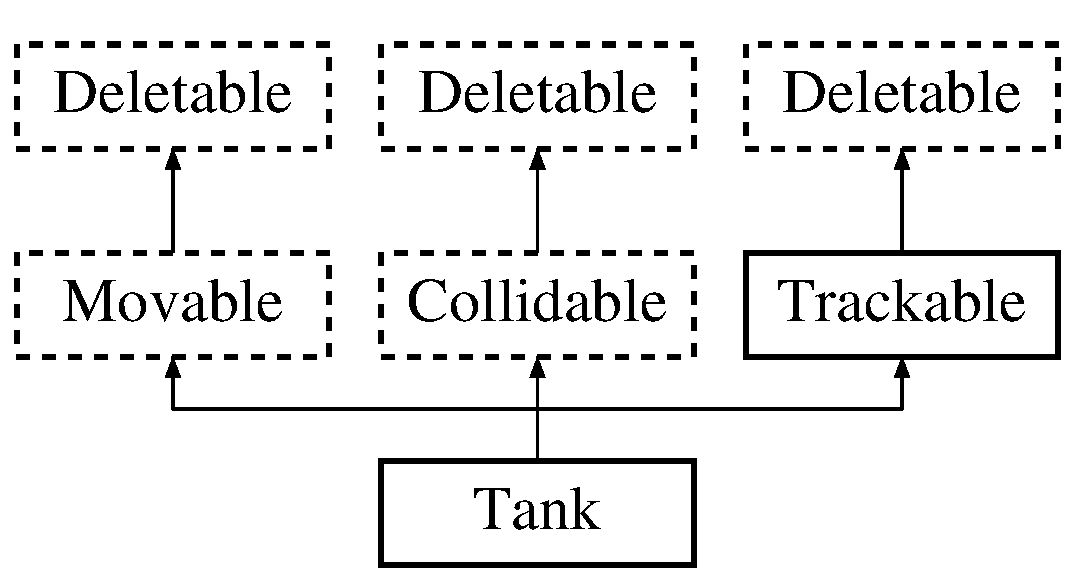
\includegraphics[height=3.000000cm]{classTank}
\end{center}
\end{figure}
\subsection*{Public Member Functions}
\begin{DoxyCompactItemize}
\item 
\hyperlink{classTank_a6150bd84a309e15815122a050972ada3}{Tank} (float position\-X, float position\-Y, float rotation, \hyperlink{Structures_8h_a6d8f83e710b27d4f86c45f0bb77066e3}{entity\-\_\-type} tank\-Owner)
\begin{DoxyCompactList}\small\item\em Default \hyperlink{classTank}{Tank} object constructor. \end{DoxyCompactList}\item 
virtual const \hyperlink{Structures_8h_a6d8f83e710b27d4f86c45f0bb77066e3}{entity\-\_\-type} \& \hyperlink{classTank_a13af6c47c61682ebd1463fd9ef34439b}{get\-Type} () const 
\begin{DoxyCompactList}\small\item\em Provided ownership. \end{DoxyCompactList}\item 
virtual void \hyperlink{classTank_a7d4317a50c215c97679cf9d2fb40e223}{move\-Forward} ()
\begin{DoxyCompactList}\small\item\em Forward movement for a tank entity. \end{DoxyCompactList}\item 
virtual void \hyperlink{classTank_a6fa5abbf02267f1e30e485b043abc1c2}{move\-Backward} ()
\begin{DoxyCompactList}\small\item\em Backward movement for a tank entity. \end{DoxyCompactList}\item 
virtual void \hyperlink{classTank_aed009351545e9019140e75bd8365e1ad}{rotate\-Left} ()
\begin{DoxyCompactList}\small\item\em Left rotation for a tank entity. \end{DoxyCompactList}\item 
virtual void \hyperlink{classTank_a61c8d236aa98a258276654d02820966f}{rotate\-Right} ()
\begin{DoxyCompactList}\small\item\em Right rotation for a tank entity. \end{DoxyCompactList}\item 
virtual const \hyperlink{structrect__corners}{rect\-\_\-corners} \& \hyperlink{classTank_aeed31f7dcffb3209928a6774c9ec2a16}{get\-Bounding\-Box} ()
\begin{DoxyCompactList}\small\item\em Provide the bounding box for the tank entity. \end{DoxyCompactList}\item 
virtual const \hyperlink{structrect__corners}{rect\-\_\-corners} \& \hyperlink{classTank_acacf07f1695303387f1f6b52fd2e2abb}{get\-Aligned\-Bounding\-Box} ()
\begin{DoxyCompactList}\small\item\em Get Axis Aligned bounding box of entity. \end{DoxyCompactList}\item 
virtual const int \hyperlink{classTank_a7bedf67f1ae11382f84a3784d9324e60}{set\-Blocked} (const \hyperlink{Structures_8h_a6fef29d9424addfa69bdd2a379424896}{blocked\-\_\-status} obstruction\-\_\-type)
\begin{DoxyCompactList}\small\item\em Instruct the tank entity that it cannot move. \end{DoxyCompactList}\item 
virtual void \hyperlink{classTank_a5cbdf86621634b0c698edc5abe1a6d5b}{set\-Unblocked} ()
\begin{DoxyCompactList}\small\item\em Instruct the tank entity that it can move. \end{DoxyCompactList}\item 
virtual void \hyperlink{classTank_a6e06f183cb856f201a7e5790b852f6a6}{set\-Collided} ()
\begin{DoxyCompactList}\small\item\em Instruct the tank entity that it has collided with another object. \end{DoxyCompactList}\item 
virtual const \hyperlink{Structures_8h_a6fef29d9424addfa69bdd2a379424896}{blocked\-\_\-status} \hyperlink{classTank_a6ca225d5f7a4c3b835da4a157b86c692}{is\-Blocked} ()
\begin{DoxyCompactList}\small\item\em Determine the blocked state of the tank entity. \end{DoxyCompactList}\item 
virtual bool const \hyperlink{classTank_a33a62b283cdaf362415fad768d2f6df3}{is\-Deleted} ()
\begin{DoxyCompactList}\small\item\em Boolean state of the tank entity's life. \end{DoxyCompactList}\item 
virtual const float \hyperlink{classTank_ab1e8f987cf6702d0a5f902fcdce2dc38}{get\-Position\-X} ()
\begin{DoxyCompactList}\small\item\em Get the current x co-\/ordinate of \hyperlink{classTrackable}{Trackable} object. \end{DoxyCompactList}\item 
virtual const float \hyperlink{classTank_ac78e2f8ecc69da315f68f4244f452bde}{get\-Position\-Y} ()
\begin{DoxyCompactList}\small\item\em Get the current y co-\/ordinate of \hyperlink{classTrackable}{Trackable} object. \end{DoxyCompactList}\item 
virtual const float \hyperlink{classTank_a893bb5e1f3ac38bd2960d1f629505ea0}{get\-Orientation} ()
\begin{DoxyCompactList}\small\item\em Get the current orientation of \hyperlink{classTrackable}{Trackable} object. \end{DoxyCompactList}\item 
virtual const \hyperlink{structrect__corners}{rect\-\_\-corners} \& \hyperlink{classTank_ac3bc1fb6dc7e36c781b6cf8a29ae87eb}{get\-Tracking\-Bounding\-Box} ()
\begin{DoxyCompactList}\small\item\em Get the bounding box relevant for line-\/of-\/fire detection. \end{DoxyCompactList}\item 
virtual const float \hyperlink{classTank_a679ab65e5d46ee6e7fa5fe517101131f}{get\-Draw\-Position\-X} ()
\begin{DoxyCompactList}\small\item\em Retrieve the \hyperlink{classTank}{Tank} x Position. \end{DoxyCompactList}\item 
virtual const float \hyperlink{classTank_a5778b15fc49b6cd1086f3a80383b2a37}{get\-Draw\-Position\-Y} ()
\begin{DoxyCompactList}\small\item\em Retrieve the \hyperlink{classTank}{Tank} y Position. \end{DoxyCompactList}\item 
virtual const float \hyperlink{classTank_aa117515fda912f25f9f7d5a8ce4055d7}{get\-Draw\-Rotation} ()
\begin{DoxyCompactList}\small\item\em Recieve the \hyperlink{classTank}{Tank} rotation. \end{DoxyCompactList}\item 
virtual void \hyperlink{classTank_ae283f9665d114b742cb521acbf0897fe}{set\-Movement\-Direction} (const \hyperlink{Structures_8h_a0d0b88f27f3adf9452879b5d9f829026}{movement\-\_\-direction} Movement\-\_\-input)
\begin{DoxyCompactList}\small\item\em Set the movement direction of the entity. \end{DoxyCompactList}\item 
virtual \hyperlink{classTank_a9e4fce49ae7fe871894c1a3122c10269}{$\sim$\-Tank} ()
\begin{DoxyCompactList}\small\item\em \hyperlink{classTank}{Tank} object destructor. \end{DoxyCompactList}\end{DoxyCompactItemize}
\subsection*{Private Attributes}
\begin{DoxyCompactItemize}
\item 
\hyperlink{Structures_8h_a6fef29d9424addfa69bdd2a379424896}{blocked\-\_\-status} \hyperlink{classTank_a55423a404ce9c8b772462665769141a5}{\-\_\-blocked\-Status}
\begin{DoxyCompactList}\small\item\em Movability of the \hyperlink{classTank}{Tank} entity\-: 1 for blocked, 0 for free. \end{DoxyCompactList}\item 
bool \hyperlink{classTank_af2526be40c377df7652b5d7c314c7861}{\-\_\-collided\-Status}
\begin{DoxyCompactList}\small\item\em Collision state of the \hyperlink{classTank}{Tank} Entity\-: 1 for collided, 0 for not. \end{DoxyCompactList}\item 
float \hyperlink{classTank_a2fe3c5fe01a1faadae727c6a667b7cc9}{\-\_\-rotation}
\begin{DoxyCompactList}\small\item\em The angle of rotation for the \hyperlink{classTank}{Tank} entity. \end{DoxyCompactList}\item 
\hyperlink{classOrientation}{Orientation} \hyperlink{classTank_ab54320f716bcac8aa4073aab09fc958b}{\-\_\-tank}
\begin{DoxyCompactList}\small\item\em Co-\/ordinate system for the \hyperlink{classTank}{Tank}. \end{DoxyCompactList}\item 
\hyperlink{Structures_8h_a6d8f83e710b27d4f86c45f0bb77066e3}{entity\-\_\-type} \hyperlink{classTank_a3758229ef9d41d069e6128b17d414204}{\-\_\-type}
\begin{DoxyCompactList}\small\item\em Enumeration type defining the tank. \end{DoxyCompactList}\item 
\hyperlink{classSpriteDimensions}{Sprite\-Dimensions} \hyperlink{classTank_ae63c3e90ba5e3f9a3bfb8172865716fb}{\-\_\-sprite\-\_\-dimensions}
\begin{DoxyCompactList}\small\item\em \hyperlink{classTank}{Tank} Sprite Dimensions. \end{DoxyCompactList}\end{DoxyCompactItemize}
\subsection*{Additional Inherited Members}


\subsection{Detailed Description}


Definition at line 29 of file Tank.\-h.



\subsection{Constructor \& Destructor Documentation}
\hypertarget{classTank_a6150bd84a309e15815122a050972ada3}{\index{Tank@{Tank}!Tank@{Tank}}
\index{Tank@{Tank}!Tank@{Tank}}
\subsubsection[{Tank}]{\setlength{\rightskip}{0pt plus 5cm}Tank\-::\-Tank (
\begin{DoxyParamCaption}
\item[{float}]{position\-X, }
\item[{float}]{position\-Y, }
\item[{float}]{rotation, }
\item[{{\bf entity\-\_\-type}}]{tank\-Owner}
\end{DoxyParamCaption}
)}}\label{classTank_a6150bd84a309e15815122a050972ada3}


Default \hyperlink{classTank}{Tank} object constructor. 

Constuctor of the \hyperlink{classTank}{Tank} Class.

This constructor utilises excetion handling and seeks to ensure that its state is invariant. 
\begin{DoxyParams}{Parameters}
{\em position\-X} & \-:\-: The initial x-\/axis to construct the tank on. \\
\hline
{\em position\-Y} & \-:\-: The initial y-\/axis to construct the tank on \\
\hline
{\em rotation} & \-:\-: The initial rotation to construct the tank with \\
\hline
{\em tank\-Owner} & \-:\-: used to set the owner of the tank as either p1 or p2 \\
\hline
\end{DoxyParams}


Definition at line 20 of file Tank.\-cpp.



References \-\_\-blocked\-Status, \-\_\-collided\-Status, \-\_\-sprite\-\_\-dimensions, \-\_\-tank, \-\_\-type, Orientation\-::get\-Origin\-X(), Orientation\-::get\-Origin\-Y(), Orientation\-::get\-Rotation(), p1\-\_\-tank, p2\-\_\-tank, Orientation\-::set\-Height(), Orientation\-::set\-Width(), Sprite\-Dimensions\-::tank\-\_\-sprite\-\_\-x, Sprite\-Dimensions\-::tank\-\_\-sprite\-\_\-y, and unblocked.


\begin{DoxyCode}
20                                                                                  :
21     \hyperlink{classTank_a2fe3c5fe01a1faadae727c6a667b7cc9}{\_rotation}(rotation),
22     \hyperlink{classTank_a3758229ef9d41d069e6128b17d414204}{\_type}(tankOwner),
23     \hyperlink{classTank_ab54320f716bcac8aa4073aab09fc958b}{\_tank}(positionX,positionY,0,0,rotation, \textcolor{keyword}{true}),
24     \hyperlink{classTank_ae63c3e90ba5e3f9a3bfb8172865716fb}{\_sprite\_dimensions}()
25 \{
26     \textcolor{comment}{//Error input checking}
27     \textcolor{keywordflow}{if} (\hyperlink{classTank_ab54320f716bcac8aa4073aab09fc958b}{\_tank}.\hyperlink{classOrientation_a4d6b853f2ac00965d29e5bc36b94c949}{getOriginX}() < 0) \textcolor{keywordflow}{throw} 
      \hyperlink{classInvalidConstructorArgumentsTank}{InvalidConstructorArgumentsTank}();
28     \textcolor{keywordflow}{if} (\hyperlink{classTank_ab54320f716bcac8aa4073aab09fc958b}{\_tank}.\hyperlink{classOrientation_ae60c88b0525d6e536a1a068d3a99f74c}{getOriginY}() < 0) \textcolor{keywordflow}{throw} 
      \hyperlink{classInvalidConstructorArgumentsTank}{InvalidConstructorArgumentsTank}();
29     \textcolor{keywordflow}{if} (\hyperlink{classTank_ab54320f716bcac8aa4073aab09fc958b}{\_tank}.\hyperlink{classOrientation_ab3568e037a7dc7799d557f2bc6a3cf7d}{getRotation}() < 0) \textcolor{keywordflow}{throw} 
      \hyperlink{classInvalidConstructorArgumentsTank}{InvalidConstructorArgumentsTank}();
30     \textcolor{keywordflow}{if} ((\hyperlink{classTank_a3758229ef9d41d069e6128b17d414204}{\_type} != \hyperlink{Structures_8h_a6d8f83e710b27d4f86c45f0bb77066e3a31fa78b2b7dd774f5158a16ef230932e}{p1\_tank}) && (\hyperlink{classTank_a3758229ef9d41d069e6128b17d414204}{\_type} != \hyperlink{Structures_8h_a6d8f83e710b27d4f86c45f0bb77066e3a3d48d62c7b88e7ee171698fe56dc9e59}{p2\_tank})) \textcolor{keywordflow}{throw} 
      \hyperlink{classInvalidConstructorArgumentsTank}{InvalidConstructorArgumentsTank}();
31 
32     \hyperlink{classTank_ab54320f716bcac8aa4073aab09fc958b}{\_tank}.\hyperlink{classOrientation_a1b5cd490e5bbbe2b8d683be389dbcbbe}{setWidth}(\hyperlink{classTank_ae63c3e90ba5e3f9a3bfb8172865716fb}{\_sprite\_dimensions}.
      \hyperlink{classSpriteDimensions_a9d7ddd6f707798f86ced573e28f9eea0}{tank\_sprite\_x});
33     \hyperlink{classTank_ab54320f716bcac8aa4073aab09fc958b}{\_tank}.\hyperlink{classOrientation_a1adca89bc32128e2ca1cb937357f5006}{setHeight}(\hyperlink{classTank_ae63c3e90ba5e3f9a3bfb8172865716fb}{\_sprite\_dimensions}.
      \hyperlink{classSpriteDimensions_abe1930e59ce44b9bdc0e6b363b668f7d}{tank\_sprite\_y});
34     \hyperlink{classTank_a55423a404ce9c8b772462665769141a5}{\_blockedStatus} = \hyperlink{Structures_8h_a6fef29d9424addfa69bdd2a379424896a1596fbf6035468467c790068b609ced3}{unblocked};
35     \hyperlink{classTank_af2526be40c377df7652b5d7c314c7861}{\_collidedStatus} = 0;
36 \}
\end{DoxyCode}
\hypertarget{classTank_a9e4fce49ae7fe871894c1a3122c10269}{\index{Tank@{Tank}!$\sim$\-Tank@{$\sim$\-Tank}}
\index{$\sim$\-Tank@{$\sim$\-Tank}!Tank@{Tank}}
\subsubsection[{$\sim$\-Tank}]{\setlength{\rightskip}{0pt plus 5cm}Tank\-::$\sim$\-Tank (
\begin{DoxyParamCaption}
{}
\end{DoxyParamCaption}
)\hspace{0.3cm}{\ttfamily [virtual]}}}\label{classTank_a9e4fce49ae7fe871894c1a3122c10269}


\hyperlink{classTank}{Tank} object destructor. 



Definition at line 186 of file Tank.\-cpp.


\begin{DoxyCode}
187 \{
188 
189 \}
\end{DoxyCode}


\subsection{Member Function Documentation}
\hypertarget{classTank_acacf07f1695303387f1f6b52fd2e2abb}{\index{Tank@{Tank}!get\-Aligned\-Bounding\-Box@{get\-Aligned\-Bounding\-Box}}
\index{get\-Aligned\-Bounding\-Box@{get\-Aligned\-Bounding\-Box}!Tank@{Tank}}
\subsubsection[{get\-Aligned\-Bounding\-Box}]{\setlength{\rightskip}{0pt plus 5cm}const {\bf rect\-\_\-corners} \& Tank\-::get\-Aligned\-Bounding\-Box (
\begin{DoxyParamCaption}
{}
\end{DoxyParamCaption}
)\hspace{0.3cm}{\ttfamily [virtual]}}}\label{classTank_acacf07f1695303387f1f6b52fd2e2abb}


Get Axis Aligned bounding box of entity. 



Implements \hyperlink{classCollidable_a6909df57a0915f044d5d967a3be086f3}{Collidable}.



Definition at line 156 of file Tank.\-cpp.



References \-\_\-tank, and Orientation\-::get\-Aligned\-Global\-Bounds().


\begin{DoxyCode}
157  \{
158      \textcolor{keywordflow}{return} \hyperlink{classTank_ab54320f716bcac8aa4073aab09fc958b}{\_tank}.\hyperlink{classOrientation_a5cc606289f774c8561af98d183586199}{getAlignedGlobalBounds}();
159  \}
\end{DoxyCode}
\hypertarget{classTank_aeed31f7dcffb3209928a6774c9ec2a16}{\index{Tank@{Tank}!get\-Bounding\-Box@{get\-Bounding\-Box}}
\index{get\-Bounding\-Box@{get\-Bounding\-Box}!Tank@{Tank}}
\subsubsection[{get\-Bounding\-Box}]{\setlength{\rightskip}{0pt plus 5cm}const {\bf rect\-\_\-corners} \& Tank\-::get\-Bounding\-Box (
\begin{DoxyParamCaption}
{}
\end{DoxyParamCaption}
)\hspace{0.3cm}{\ttfamily [virtual]}}}\label{classTank_aeed31f7dcffb3209928a6774c9ec2a16}


Provide the bounding box for the tank entity. 

Retrieves the tanks bounding box.

This function is used in conjunction with collision detection 

Implements \hyperlink{classCollidable_a3436effdcd9bea230f4a1aa32b8dd8ab}{Collidable}.



Definition at line 91 of file Tank.\-cpp.



References \-\_\-tank, and Orientation\-::get\-Global\-Bounds().


\begin{DoxyCode}
92 \{
93     \textcolor{keywordflow}{return} \hyperlink{classTank_ab54320f716bcac8aa4073aab09fc958b}{\_tank}.\hyperlink{classOrientation_a950dfe84e548582d8c3c573b5ff5fe42}{getGlobalBounds}();
94 \}
\end{DoxyCode}
\hypertarget{classTank_a679ab65e5d46ee6e7fa5fe517101131f}{\index{Tank@{Tank}!get\-Draw\-Position\-X@{get\-Draw\-Position\-X}}
\index{get\-Draw\-Position\-X@{get\-Draw\-Position\-X}!Tank@{Tank}}
\subsubsection[{get\-Draw\-Position\-X}]{\setlength{\rightskip}{0pt plus 5cm}const float Tank\-::get\-Draw\-Position\-X (
\begin{DoxyParamCaption}
{}
\end{DoxyParamCaption}
)\hspace{0.3cm}{\ttfamily [virtual]}}}\label{classTank_a679ab65e5d46ee6e7fa5fe517101131f}


Retrieve the \hyperlink{classTank}{Tank} x Position. 

Retrieve the x \hyperlink{classTank}{Tank} Position. 

Implements \hyperlink{classDeletable_ac14ea0c5986d50ba3ba454f89c87b8fe}{Deletable}.



Definition at line 162 of file Tank.\-cpp.



References \-\_\-tank, and Orientation\-::get\-Origin\-X().



Referenced by T\-E\-S\-T().


\begin{DoxyCode}
163 \{
164     \textcolor{keywordflow}{return} \hyperlink{classTank_ab54320f716bcac8aa4073aab09fc958b}{\_tank}.\hyperlink{classOrientation_a4d6b853f2ac00965d29e5bc36b94c949}{getOriginX}();
165 \}
\end{DoxyCode}
\hypertarget{classTank_a5778b15fc49b6cd1086f3a80383b2a37}{\index{Tank@{Tank}!get\-Draw\-Position\-Y@{get\-Draw\-Position\-Y}}
\index{get\-Draw\-Position\-Y@{get\-Draw\-Position\-Y}!Tank@{Tank}}
\subsubsection[{get\-Draw\-Position\-Y}]{\setlength{\rightskip}{0pt plus 5cm}const float Tank\-::get\-Draw\-Position\-Y (
\begin{DoxyParamCaption}
{}
\end{DoxyParamCaption}
)\hspace{0.3cm}{\ttfamily [virtual]}}}\label{classTank_a5778b15fc49b6cd1086f3a80383b2a37}


Retrieve the \hyperlink{classTank}{Tank} y Position. 

Retrieve the y \hyperlink{classTank}{Tank} Position. 

Implements \hyperlink{classDeletable_a2a88d7e40c56902a3d3d8f668e9d126d}{Deletable}.



Definition at line 168 of file Tank.\-cpp.



References \-\_\-tank, and Orientation\-::get\-Origin\-Y().



Referenced by T\-E\-S\-T().


\begin{DoxyCode}
169 \{
170     \textcolor{keywordflow}{return} \hyperlink{classTank_ab54320f716bcac8aa4073aab09fc958b}{\_tank}.\hyperlink{classOrientation_ae60c88b0525d6e536a1a068d3a99f74c}{getOriginY}();
171 \}
\end{DoxyCode}
\hypertarget{classTank_aa117515fda912f25f9f7d5a8ce4055d7}{\index{Tank@{Tank}!get\-Draw\-Rotation@{get\-Draw\-Rotation}}
\index{get\-Draw\-Rotation@{get\-Draw\-Rotation}!Tank@{Tank}}
\subsubsection[{get\-Draw\-Rotation}]{\setlength{\rightskip}{0pt plus 5cm}const float Tank\-::get\-Draw\-Rotation (
\begin{DoxyParamCaption}
{}
\end{DoxyParamCaption}
)\hspace{0.3cm}{\ttfamily [virtual]}}}\label{classTank_aa117515fda912f25f9f7d5a8ce4055d7}


Recieve the \hyperlink{classTank}{Tank} rotation. 



Implements \hyperlink{classDeletable_ad7061a6bef3efce030aa5abbc7646d47}{Deletable}.



Definition at line 174 of file Tank.\-cpp.



References \-\_\-tank, and Orientation\-::get\-Rotation().



Referenced by T\-E\-S\-T().


\begin{DoxyCode}
175 \{
176     \textcolor{keywordflow}{return} \hyperlink{classTank_ab54320f716bcac8aa4073aab09fc958b}{\_tank}.\hyperlink{classOrientation_ab3568e037a7dc7799d557f2bc6a3cf7d}{getRotation}();
177 \}
\end{DoxyCode}
\hypertarget{classTank_a893bb5e1f3ac38bd2960d1f629505ea0}{\index{Tank@{Tank}!get\-Orientation@{get\-Orientation}}
\index{get\-Orientation@{get\-Orientation}!Tank@{Tank}}
\subsubsection[{get\-Orientation}]{\setlength{\rightskip}{0pt plus 5cm}const float Tank\-::get\-Orientation (
\begin{DoxyParamCaption}
{}
\end{DoxyParamCaption}
)\hspace{0.3cm}{\ttfamily [virtual]}}}\label{classTank_a893bb5e1f3ac38bd2960d1f629505ea0}


Get the current orientation of \hyperlink{classTrackable}{Trackable} object. 



Implements \hyperlink{classTrackable_afc6b5126b82395a5155cfe76250f92dd}{Trackable}.



Definition at line 145 of file Tank.\-cpp.



References \-\_\-tank, and Orientation\-::get\-Rotation().



Referenced by T\-E\-S\-T().


\begin{DoxyCode}
146 \{
147     \textcolor{keywordflow}{return} \hyperlink{classTank_ab54320f716bcac8aa4073aab09fc958b}{\_tank}.\hyperlink{classOrientation_ab3568e037a7dc7799d557f2bc6a3cf7d}{getRotation}();
148 \}
\end{DoxyCode}
\hypertarget{classTank_ab1e8f987cf6702d0a5f902fcdce2dc38}{\index{Tank@{Tank}!get\-Position\-X@{get\-Position\-X}}
\index{get\-Position\-X@{get\-Position\-X}!Tank@{Tank}}
\subsubsection[{get\-Position\-X}]{\setlength{\rightskip}{0pt plus 5cm}const float Tank\-::get\-Position\-X (
\begin{DoxyParamCaption}
{}
\end{DoxyParamCaption}
)\hspace{0.3cm}{\ttfamily [virtual]}}}\label{classTank_ab1e8f987cf6702d0a5f902fcdce2dc38}


Get the current x co-\/ordinate of \hyperlink{classTrackable}{Trackable} object. 

Get the current x co-\/ordinates of \hyperlink{classTrackable}{Trackable} object. 

Implements \hyperlink{classTrackable_ab167af97aef9656403ee2d28adaf3149}{Trackable}.



Definition at line 133 of file Tank.\-cpp.



References \-\_\-tank, and Orientation\-::get\-Origin\-X().



Referenced by T\-E\-S\-T().


\begin{DoxyCode}
134 \{
135     \textcolor{keywordflow}{return} \hyperlink{classTank_ab54320f716bcac8aa4073aab09fc958b}{\_tank}.\hyperlink{classOrientation_a4d6b853f2ac00965d29e5bc36b94c949}{getOriginX}();
136 \}
\end{DoxyCode}
\hypertarget{classTank_ac78e2f8ecc69da315f68f4244f452bde}{\index{Tank@{Tank}!get\-Position\-Y@{get\-Position\-Y}}
\index{get\-Position\-Y@{get\-Position\-Y}!Tank@{Tank}}
\subsubsection[{get\-Position\-Y}]{\setlength{\rightskip}{0pt plus 5cm}const float Tank\-::get\-Position\-Y (
\begin{DoxyParamCaption}
{}
\end{DoxyParamCaption}
)\hspace{0.3cm}{\ttfamily [virtual]}}}\label{classTank_ac78e2f8ecc69da315f68f4244f452bde}


Get the current y co-\/ordinate of \hyperlink{classTrackable}{Trackable} object. 

Get the current y co-\/ordinates of \hyperlink{classTrackable}{Trackable} object. 

Implements \hyperlink{classTrackable_add27867f4ebf30f1fe7c3f94b4d7f4d5}{Trackable}.



Definition at line 139 of file Tank.\-cpp.



References \-\_\-tank, and Orientation\-::get\-Origin\-Y().



Referenced by T\-E\-S\-T().


\begin{DoxyCode}
140 \{
141     \textcolor{keywordflow}{return} \hyperlink{classTank_ab54320f716bcac8aa4073aab09fc958b}{\_tank}.\hyperlink{classOrientation_ae60c88b0525d6e536a1a068d3a99f74c}{getOriginY}();
142 \}
\end{DoxyCode}
\hypertarget{classTank_ac3bc1fb6dc7e36c781b6cf8a29ae87eb}{\index{Tank@{Tank}!get\-Tracking\-Bounding\-Box@{get\-Tracking\-Bounding\-Box}}
\index{get\-Tracking\-Bounding\-Box@{get\-Tracking\-Bounding\-Box}!Tank@{Tank}}
\subsubsection[{get\-Tracking\-Bounding\-Box}]{\setlength{\rightskip}{0pt plus 5cm}const {\bf rect\-\_\-corners} \& Tank\-::get\-Tracking\-Bounding\-Box (
\begin{DoxyParamCaption}
{}
\end{DoxyParamCaption}
)\hspace{0.3cm}{\ttfamily [virtual]}}}\label{classTank_ac3bc1fb6dc7e36c781b6cf8a29ae87eb}


Get the bounding box relevant for line-\/of-\/fire detection. 



Implements \hyperlink{classTrackable_a79826040547e1ca65775223f26c37648}{Trackable}.



Definition at line 151 of file Tank.\-cpp.



References \-\_\-tank, and Orientation\-::get\-Global\-Bounds().


\begin{DoxyCode}
152  \{
153     \textcolor{keywordflow}{return} \hyperlink{classTank_ab54320f716bcac8aa4073aab09fc958b}{\_tank}.\hyperlink{classOrientation_a950dfe84e548582d8c3c573b5ff5fe42}{getGlobalBounds}();
154  \}
\end{DoxyCode}
\hypertarget{classTank_a13af6c47c61682ebd1463fd9ef34439b}{\index{Tank@{Tank}!get\-Type@{get\-Type}}
\index{get\-Type@{get\-Type}!Tank@{Tank}}
\subsubsection[{get\-Type}]{\setlength{\rightskip}{0pt plus 5cm}const {\bf entity\-\_\-type} \& Tank\-::get\-Type (
\begin{DoxyParamCaption}
{}
\end{DoxyParamCaption}
) const\hspace{0.3cm}{\ttfamily [virtual]}}}\label{classTank_a13af6c47c61682ebd1463fd9ef34439b}


Provided ownership. 

Returns the owner of the tank.

This is function is used in many logic instanses where the owner of the tank needs to be determined. \begin{DoxyReturn}{Returns}
entity\-\_\-type 
\end{DoxyReturn}


Implements \hyperlink{classDeletable_af8a0208abc297180873692f4215fe50f}{Deletable}.



Definition at line 44 of file Tank.\-cpp.



References \-\_\-type.



Referenced by T\-E\-S\-T().


\begin{DoxyCode}
45  \{
46      \textcolor{keywordflow}{return} \hyperlink{classTank_a3758229ef9d41d069e6128b17d414204}{\_type};
47  \}
\end{DoxyCode}
\hypertarget{classTank_a6ca225d5f7a4c3b835da4a157b86c692}{\index{Tank@{Tank}!is\-Blocked@{is\-Blocked}}
\index{is\-Blocked@{is\-Blocked}!Tank@{Tank}}
\subsubsection[{is\-Blocked}]{\setlength{\rightskip}{0pt plus 5cm}const {\bf blocked\-\_\-status} Tank\-::is\-Blocked (
\begin{DoxyParamCaption}
{}
\end{DoxyParamCaption}
)\hspace{0.3cm}{\ttfamily [virtual]}}}\label{classTank_a6ca225d5f7a4c3b835da4a157b86c692}


Determine the blocked state of the tank entity. 



Implements \hyperlink{classMovable_a40db320f27f5be1882553298677702c8}{Movable}.



Definition at line 121 of file Tank.\-cpp.



References \-\_\-blocked\-Status.



Referenced by T\-E\-S\-T().


\begin{DoxyCode}
122 \{
123     \textcolor{keywordflow}{return} \hyperlink{classTank_a55423a404ce9c8b772462665769141a5}{\_blockedStatus};
124 \}
\end{DoxyCode}
\hypertarget{classTank_a33a62b283cdaf362415fad768d2f6df3}{\index{Tank@{Tank}!is\-Deleted@{is\-Deleted}}
\index{is\-Deleted@{is\-Deleted}!Tank@{Tank}}
\subsubsection[{is\-Deleted}]{\setlength{\rightskip}{0pt plus 5cm}const bool Tank\-::is\-Deleted (
\begin{DoxyParamCaption}
{}
\end{DoxyParamCaption}
)\hspace{0.3cm}{\ttfamily [virtual]}}}\label{classTank_a33a62b283cdaf362415fad768d2f6df3}


Boolean state of the tank entity's life. 



Implements \hyperlink{classDeletable_a6572440c291077cf52bf21288c6cd25c}{Deletable}.



Definition at line 127 of file Tank.\-cpp.



References \-\_\-collided\-Status.



Referenced by T\-E\-S\-T().


\begin{DoxyCode}
128 \{
129     \textcolor{keywordflow}{return} \hyperlink{classTank_af2526be40c377df7652b5d7c314c7861}{\_collidedStatus};
130 \}
\end{DoxyCode}
\hypertarget{classTank_a6fa5abbf02267f1e30e485b043abc1c2}{\index{Tank@{Tank}!move\-Backward@{move\-Backward}}
\index{move\-Backward@{move\-Backward}!Tank@{Tank}}
\subsubsection[{move\-Backward}]{\setlength{\rightskip}{0pt plus 5cm}void Tank\-::move\-Backward (
\begin{DoxyParamCaption}
{}
\end{DoxyParamCaption}
)\hspace{0.3cm}{\ttfamily [virtual]}}}\label{classTank_a6fa5abbf02267f1e30e485b043abc1c2}


Backward movement for a tank entity. 

Moves the tank forward by a constant value.

This method uses trigonometry to move the tank negatively in any 360 degree direction within the game world 

Implements \hyperlink{classMovable_a9c03e7ac263902159579d7f83e9b6dee}{Movable}.



Definition at line 63 of file Tank.\-cpp.



References \-\_\-rotation, \-\_\-tank, Movable\-::\-\_\-tank\-Movement\-Speed, Orientation\-::move(), and P\-I.



Referenced by T\-E\-S\-T().


\begin{DoxyCode}
64 \{
65     \hyperlink{classTank_ab54320f716bcac8aa4073aab09fc958b}{\_tank}.\hyperlink{classOrientation_ae1c8122591724b1b3bfcb0026b76e809}{move}(-\hyperlink{classMovable_a54cb7d3465cc78ad7d8b2f7c2d842732}{\_tankMovementSpeed}*cos((\hyperlink{classTank_a2fe3c5fe01a1faadae727c6a667b7cc9}{\_rotation}*
      \hyperlink{ClassTests_8cpp_a598a3330b3c21701223ee0ca14316eca}{PI})/180.0), -\hyperlink{classMovable_a54cb7d3465cc78ad7d8b2f7c2d842732}{\_tankMovementSpeed}*sin((\hyperlink{classTank_a2fe3c5fe01a1faadae727c6a667b7cc9}{\_rotation}*PI)/180.0));
66 \}
\end{DoxyCode}
\hypertarget{classTank_a7d4317a50c215c97679cf9d2fb40e223}{\index{Tank@{Tank}!move\-Forward@{move\-Forward}}
\index{move\-Forward@{move\-Forward}!Tank@{Tank}}
\subsubsection[{move\-Forward}]{\setlength{\rightskip}{0pt plus 5cm}void Tank\-::move\-Forward (
\begin{DoxyParamCaption}
{}
\end{DoxyParamCaption}
)\hspace{0.3cm}{\ttfamily [virtual]}}}\label{classTank_a7d4317a50c215c97679cf9d2fb40e223}


Forward movement for a tank entity. 

Moves the tank forward by a constant value.

This method uses trigonometry to move the tank positively in any 360 degree direction within the game world 

Implements \hyperlink{classMovable_adefaf61339698c5efec597529bf89310}{Movable}.



Definition at line 53 of file Tank.\-cpp.



References \-\_\-rotation, \-\_\-tank, Movable\-::\-\_\-tank\-Movement\-Speed, Orientation\-::move(), and P\-I.



Referenced by T\-E\-S\-T().


\begin{DoxyCode}
54 \{
55     \hyperlink{classTank_ab54320f716bcac8aa4073aab09fc958b}{\_tank}.\hyperlink{classOrientation_ae1c8122591724b1b3bfcb0026b76e809}{move}(\hyperlink{classMovable_a54cb7d3465cc78ad7d8b2f7c2d842732}{\_tankMovementSpeed}*cos((\hyperlink{classTank_a2fe3c5fe01a1faadae727c6a667b7cc9}{\_rotation}*
      \hyperlink{ClassTests_8cpp_a598a3330b3c21701223ee0ca14316eca}{PI})/180.0), \hyperlink{classMovable_a54cb7d3465cc78ad7d8b2f7c2d842732}{\_tankMovementSpeed}*sin((\hyperlink{classTank_a2fe3c5fe01a1faadae727c6a667b7cc9}{\_rotation}*PI)/180.0));
56 \}
\end{DoxyCode}
\hypertarget{classTank_aed009351545e9019140e75bd8365e1ad}{\index{Tank@{Tank}!rotate\-Left@{rotate\-Left}}
\index{rotate\-Left@{rotate\-Left}!Tank@{Tank}}
\subsubsection[{rotate\-Left}]{\setlength{\rightskip}{0pt plus 5cm}void Tank\-::rotate\-Left (
\begin{DoxyParamCaption}
{}
\end{DoxyParamCaption}
)\hspace{0.3cm}{\ttfamily [virtual]}}}\label{classTank_aed009351545e9019140e75bd8365e1ad}


Left rotation for a tank entity. 

Rotates the tank left by a constant value.

This method uses trigonometry to move the tank positively in any degree if rotation 

Implements \hyperlink{classMovable_a422b71ade02b9034600f51bc55d58c90}{Movable}.



Definition at line 71 of file Tank.\-cpp.



References \-\_\-rotation, \-\_\-tank, Movable\-::\-\_\-tank\-Rotation\-Speed, and Orientation\-::rotate().



Referenced by T\-E\-S\-T().


\begin{DoxyCode}
72 \{
73     \hyperlink{classTank_a2fe3c5fe01a1faadae727c6a667b7cc9}{\_rotation} += \hyperlink{classMovable_ab4ad35a0057bdbc80385c67bec5f1a60}{\_tankRotationSpeed};
74     \hyperlink{classTank_ab54320f716bcac8aa4073aab09fc958b}{\_tank}.\hyperlink{classOrientation_aa9e115b7f4ab487e3af532592416b247}{rotate}(\hyperlink{classMovable_ab4ad35a0057bdbc80385c67bec5f1a60}{\_tankRotationSpeed});
75 \}
\end{DoxyCode}
\hypertarget{classTank_a61c8d236aa98a258276654d02820966f}{\index{Tank@{Tank}!rotate\-Right@{rotate\-Right}}
\index{rotate\-Right@{rotate\-Right}!Tank@{Tank}}
\subsubsection[{rotate\-Right}]{\setlength{\rightskip}{0pt plus 5cm}void Tank\-::rotate\-Right (
\begin{DoxyParamCaption}
{}
\end{DoxyParamCaption}
)\hspace{0.3cm}{\ttfamily [virtual]}}}\label{classTank_a61c8d236aa98a258276654d02820966f}


Right rotation for a tank entity. 

Rotates the tank right by a constant value.

This method uses trigonometry to move the tank negatively in any degree if rotation 

Implements \hyperlink{classMovable_a821480cb8ffd047b39a907c6cf07dd84}{Movable}.



Definition at line 81 of file Tank.\-cpp.



References \-\_\-rotation, \-\_\-tank, Movable\-::\-\_\-tank\-Rotation\-Speed, and Orientation\-::rotate().



Referenced by T\-E\-S\-T().


\begin{DoxyCode}
82 \{
83     \hyperlink{classTank_a2fe3c5fe01a1faadae727c6a667b7cc9}{\_rotation} -= \hyperlink{classMovable_ab4ad35a0057bdbc80385c67bec5f1a60}{\_tankRotationSpeed};
84     \hyperlink{classTank_ab54320f716bcac8aa4073aab09fc958b}{\_tank}.\hyperlink{classOrientation_aa9e115b7f4ab487e3af532592416b247}{rotate}(-\hyperlink{classMovable_ab4ad35a0057bdbc80385c67bec5f1a60}{\_tankRotationSpeed});
85 \}
\end{DoxyCode}
\hypertarget{classTank_a7bedf67f1ae11382f84a3784d9324e60}{\index{Tank@{Tank}!set\-Blocked@{set\-Blocked}}
\index{set\-Blocked@{set\-Blocked}!Tank@{Tank}}
\subsubsection[{set\-Blocked}]{\setlength{\rightskip}{0pt plus 5cm}const int Tank\-::set\-Blocked (
\begin{DoxyParamCaption}
\item[{const {\bf blocked\-\_\-status}}]{obstruction\-\_\-type}
\end{DoxyParamCaption}
)\hspace{0.3cm}{\ttfamily [virtual]}}}\label{classTank_a7bedf67f1ae11382f84a3784d9324e60}


Instruct the tank entity that it cannot move. 

Set the movement state of the \hyperlink{classTank}{Tank} to be blocked.

This function sets a boolean value and returns an int describing how manay more times it can be blocked 
\begin{DoxyParams}{Parameters}
{\em obstruction\-\_\-type} & \-:\-: this is the direction in which the tank becomes blocked \\
\hline
\end{DoxyParams}


Implements \hyperlink{classCollidable_a6d312198ba82d26b5e360733bb87a2f0}{Collidable}.



Definition at line 101 of file Tank.\-cpp.



References \-\_\-blocked\-Status.



Referenced by T\-E\-S\-T().


\begin{DoxyCode}
102 \{
103     \hyperlink{classTank_a55423a404ce9c8b772462665769141a5}{\_blockedStatus} = obstruction\_type;
104     \textcolor{comment}{//Tank intity can be blocked infinitely.}
105     \textcolor{keywordflow}{return} 1;
106 \}
\end{DoxyCode}
\hypertarget{classTank_a6e06f183cb856f201a7e5790b852f6a6}{\index{Tank@{Tank}!set\-Collided@{set\-Collided}}
\index{set\-Collided@{set\-Collided}!Tank@{Tank}}
\subsubsection[{set\-Collided}]{\setlength{\rightskip}{0pt plus 5cm}void Tank\-::set\-Collided (
\begin{DoxyParamCaption}
{}
\end{DoxyParamCaption}
)\hspace{0.3cm}{\ttfamily [virtual]}}}\label{classTank_a6e06f183cb856f201a7e5790b852f6a6}


Instruct the tank entity that it has collided with another object. 



Implements \hyperlink{classCollidable_a5ea0417bea000712171bbe5531705082}{Collidable}.



Definition at line 115 of file Tank.\-cpp.



References \-\_\-collided\-Status.



Referenced by T\-E\-S\-T().


\begin{DoxyCode}
116 \{
117     \hyperlink{classTank_af2526be40c377df7652b5d7c314c7861}{\_collidedStatus} = 1;
118 \}
\end{DoxyCode}
\hypertarget{classTank_ae283f9665d114b742cb521acbf0897fe}{\index{Tank@{Tank}!set\-Movement\-Direction@{set\-Movement\-Direction}}
\index{set\-Movement\-Direction@{set\-Movement\-Direction}!Tank@{Tank}}
\subsubsection[{set\-Movement\-Direction}]{\setlength{\rightskip}{0pt plus 5cm}void Tank\-::set\-Movement\-Direction (
\begin{DoxyParamCaption}
\item[{const {\bf movement\-\_\-direction}}]{Movement\-\_\-input}
\end{DoxyParamCaption}
)\hspace{0.3cm}{\ttfamily [virtual]}}}\label{classTank_ae283f9665d114b742cb521acbf0897fe}


Set the movement direction of the entity. 



Implements \hyperlink{classMovable_a0bb485f10776845305a683ed5e2ba1fc}{Movable}.



Definition at line 180 of file Tank.\-cpp.



References \-\_\-tank, and Orientation\-::set\-Move\-Direction().


\begin{DoxyCode}
181 \{
182     \hyperlink{classTank_ab54320f716bcac8aa4073aab09fc958b}{\_tank}.\hyperlink{classOrientation_a478512ba497cd75f11be3aa3177cca6a}{setMoveDirection}(Movement\_input);
183 \}
\end{DoxyCode}
\hypertarget{classTank_a5cbdf86621634b0c698edc5abe1a6d5b}{\index{Tank@{Tank}!set\-Unblocked@{set\-Unblocked}}
\index{set\-Unblocked@{set\-Unblocked}!Tank@{Tank}}
\subsubsection[{set\-Unblocked}]{\setlength{\rightskip}{0pt plus 5cm}void Tank\-::set\-Unblocked (
\begin{DoxyParamCaption}
{}
\end{DoxyParamCaption}
)\hspace{0.3cm}{\ttfamily [virtual]}}}\label{classTank_a5cbdf86621634b0c698edc5abe1a6d5b}


Instruct the tank entity that it can move. 



Implements \hyperlink{classCollidable_a817d864d0640bc6bcb13bbecf14ddf31}{Collidable}.



Definition at line 109 of file Tank.\-cpp.



References \-\_\-blocked\-Status, and unblocked.



Referenced by T\-E\-S\-T().


\begin{DoxyCode}
110 \{
111     \hyperlink{classTank_a55423a404ce9c8b772462665769141a5}{\_blockedStatus} = \hyperlink{Structures_8h_a6fef29d9424addfa69bdd2a379424896a1596fbf6035468467c790068b609ced3}{unblocked};
112 \}
\end{DoxyCode}


\subsection{Member Data Documentation}
\hypertarget{classTank_a55423a404ce9c8b772462665769141a5}{\index{Tank@{Tank}!\-\_\-blocked\-Status@{\-\_\-blocked\-Status}}
\index{\-\_\-blocked\-Status@{\-\_\-blocked\-Status}!Tank@{Tank}}
\subsubsection[{\-\_\-blocked\-Status}]{\setlength{\rightskip}{0pt plus 5cm}{\bf blocked\-\_\-status} Tank\-::\-\_\-blocked\-Status\hspace{0.3cm}{\ttfamily [private]}}}\label{classTank_a55423a404ce9c8b772462665769141a5}


Movability of the \hyperlink{classTank}{Tank} entity\-: 1 for blocked, 0 for free. 



Definition at line 81 of file Tank.\-h.



Referenced by is\-Blocked(), set\-Blocked(), set\-Unblocked(), and Tank().

\hypertarget{classTank_af2526be40c377df7652b5d7c314c7861}{\index{Tank@{Tank}!\-\_\-collided\-Status@{\-\_\-collided\-Status}}
\index{\-\_\-collided\-Status@{\-\_\-collided\-Status}!Tank@{Tank}}
\subsubsection[{\-\_\-collided\-Status}]{\setlength{\rightskip}{0pt plus 5cm}bool Tank\-::\-\_\-collided\-Status\hspace{0.3cm}{\ttfamily [private]}}}\label{classTank_af2526be40c377df7652b5d7c314c7861}


Collision state of the \hyperlink{classTank}{Tank} Entity\-: 1 for collided, 0 for not. 



Definition at line 83 of file Tank.\-h.



Referenced by is\-Deleted(), set\-Collided(), and Tank().

\hypertarget{classTank_a2fe3c5fe01a1faadae727c6a667b7cc9}{\index{Tank@{Tank}!\-\_\-rotation@{\-\_\-rotation}}
\index{\-\_\-rotation@{\-\_\-rotation}!Tank@{Tank}}
\subsubsection[{\-\_\-rotation}]{\setlength{\rightskip}{0pt plus 5cm}float Tank\-::\-\_\-rotation\hspace{0.3cm}{\ttfamily [private]}}}\label{classTank_a2fe3c5fe01a1faadae727c6a667b7cc9}


The angle of rotation for the \hyperlink{classTank}{Tank} entity. 



Definition at line 85 of file Tank.\-h.



Referenced by move\-Backward(), move\-Forward(), rotate\-Left(), and rotate\-Right().

\hypertarget{classTank_ae63c3e90ba5e3f9a3bfb8172865716fb}{\index{Tank@{Tank}!\-\_\-sprite\-\_\-dimensions@{\-\_\-sprite\-\_\-dimensions}}
\index{\-\_\-sprite\-\_\-dimensions@{\-\_\-sprite\-\_\-dimensions}!Tank@{Tank}}
\subsubsection[{\-\_\-sprite\-\_\-dimensions}]{\setlength{\rightskip}{0pt plus 5cm}{\bf Sprite\-Dimensions} Tank\-::\-\_\-sprite\-\_\-dimensions\hspace{0.3cm}{\ttfamily [private]}}}\label{classTank_ae63c3e90ba5e3f9a3bfb8172865716fb}


\hyperlink{classTank}{Tank} Sprite Dimensions. 



Definition at line 91 of file Tank.\-h.



Referenced by Tank().

\hypertarget{classTank_ab54320f716bcac8aa4073aab09fc958b}{\index{Tank@{Tank}!\-\_\-tank@{\-\_\-tank}}
\index{\-\_\-tank@{\-\_\-tank}!Tank@{Tank}}
\subsubsection[{\-\_\-tank}]{\setlength{\rightskip}{0pt plus 5cm}{\bf Orientation} Tank\-::\-\_\-tank\hspace{0.3cm}{\ttfamily [private]}}}\label{classTank_ab54320f716bcac8aa4073aab09fc958b}


Co-\/ordinate system for the \hyperlink{classTank}{Tank}. 



Definition at line 87 of file Tank.\-h.



Referenced by get\-Aligned\-Bounding\-Box(), get\-Bounding\-Box(), get\-Draw\-Position\-X(), get\-Draw\-Position\-Y(), get\-Draw\-Rotation(), get\-Orientation(), get\-Position\-X(), get\-Position\-Y(), get\-Tracking\-Bounding\-Box(), move\-Backward(), move\-Forward(), rotate\-Left(), rotate\-Right(), set\-Movement\-Direction(), and Tank().

\hypertarget{classTank_a3758229ef9d41d069e6128b17d414204}{\index{Tank@{Tank}!\-\_\-type@{\-\_\-type}}
\index{\-\_\-type@{\-\_\-type}!Tank@{Tank}}
\subsubsection[{\-\_\-type}]{\setlength{\rightskip}{0pt plus 5cm}{\bf entity\-\_\-type} Tank\-::\-\_\-type\hspace{0.3cm}{\ttfamily [private]}}}\label{classTank_a3758229ef9d41d069e6128b17d414204}


Enumeration type defining the tank. 



Definition at line 89 of file Tank.\-h.



Referenced by get\-Type(), and Tank().



The documentation for this class was generated from the following files\-:\begin{DoxyCompactItemize}
\item 
\hyperlink{Tank_8h}{Tank.\-h}\item 
\hyperlink{Tank_8cpp}{Tank.\-cpp}\end{DoxyCompactItemize}

\hypertarget{structtextures}{\section{textures Struct Reference}
\label{structtextures}\index{textures@{textures}}
}
\subsection*{Public Attributes}
\begin{DoxyCompactItemize}
\item 
\hypertarget{structtextures_a9287e247a5d108ed875b7b5b89ded524}{sf\+::\+Texture {\bfseries tank\+\_\+1}}\label{structtextures_a9287e247a5d108ed875b7b5b89ded524}

\item 
\hypertarget{structtextures_a3322b3f064640afe1a4ebdb53636b71d}{sf\+::\+Texture {\bfseries tank\+\_\+2}}\label{structtextures_a3322b3f064640afe1a4ebdb53636b71d}

\item 
\hypertarget{structtextures_a1d12557e92da80a9809f037edfe72f2f}{sf\+::\+Texture {\bfseries missile}}\label{structtextures_a1d12557e92da80a9809f037edfe72f2f}

\item 
\hypertarget{structtextures_a7f5b6643fd47d1bd8d5758c24c32dc9e}{sf\+::\+Texture {\bfseries mine}}\label{structtextures_a7f5b6643fd47d1bd8d5758c24c32dc9e}

\item 
\hypertarget{structtextures_a36f35bd26858ecc8eb507e1072bfad7d}{sf\+::\+Texture {\bfseries barrier}}\label{structtextures_a36f35bd26858ecc8eb507e1072bfad7d}

\item 
\hypertarget{structtextures_a703e4f064d67c1cee84ba8560a6104c6}{sf\+::\+Texture {\bfseries map}}\label{structtextures_a703e4f064d67c1cee84ba8560a6104c6}

\item 
\hypertarget{structtextures_a8454a0f97657e68ca0076f19c4de6236}{sf\+::\+Texture {\bfseries turret}}\label{structtextures_a8454a0f97657e68ca0076f19c4de6236}

\item 
\hypertarget{structtextures_aa9ff61d80b32b3520308d8df61a8ea3f}{sf\+::\+Texture {\bfseries turret\+\_\+missile}}\label{structtextures_aa9ff61d80b32b3520308d8df61a8ea3f}

\end{DoxyCompactItemize}


\subsection{Detailed Description}


Definition at line 68 of file Structures.\+h.



The documentation for this struct was generated from the following file\+:\begin{DoxyCompactItemize}
\item 
\hyperlink{_structures_8h}{Structures.\+h}\end{DoxyCompactItemize}

\hypertarget{classTrackable}{\section{Trackable Class Reference}
\label{classTrackable}\index{Trackable@{Trackable}}
}


An Abstract-\/based class forming an interface for all \hyperlink{classTrackable}{Trackable} objects within the game.  




{\ttfamily \#include $<$Trackable.\-h$>$}

Inheritance diagram for Trackable\-:\begin{figure}[H]
\begin{center}
\leavevmode
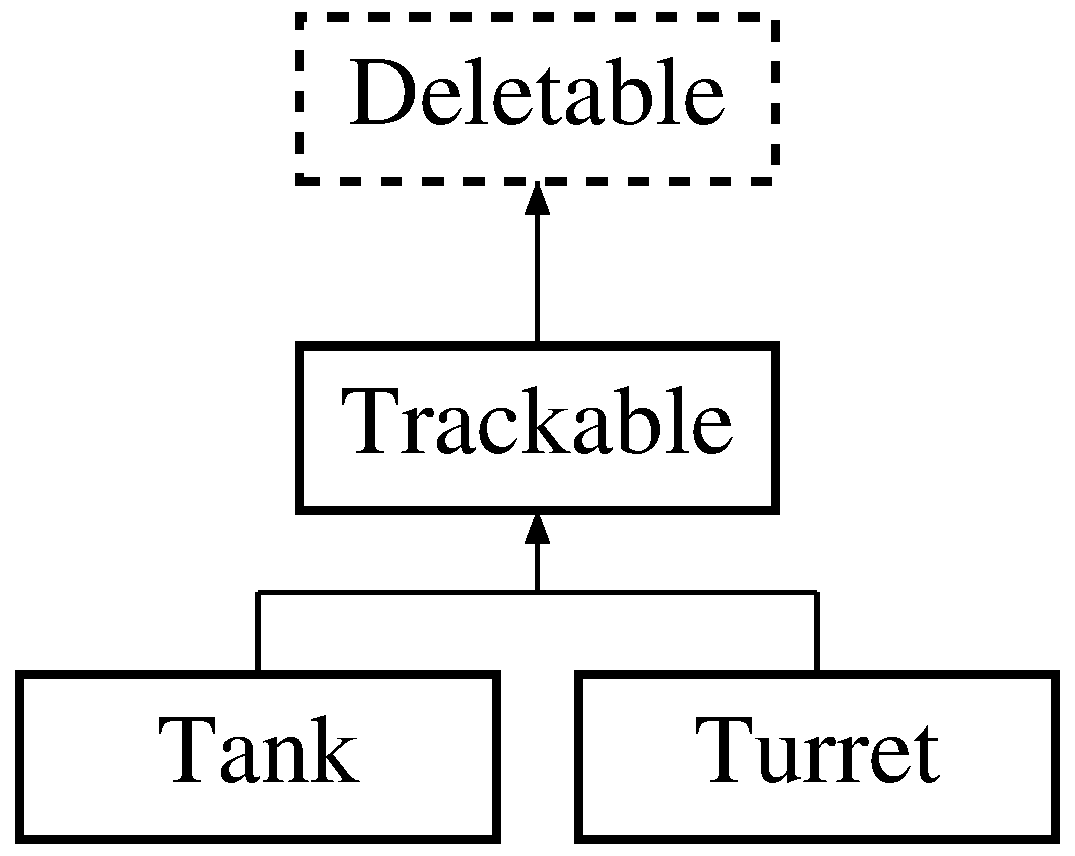
\includegraphics[height=3.000000cm]{classTrackable}
\end{center}
\end{figure}
\subsection*{Public Member Functions}
\begin{DoxyCompactItemize}
\item 
\hyperlink{classTrackable_aa95786c1de337603ffe42e74cef944e0}{Trackable} ()
\begin{DoxyCompactList}\small\item\em Constructor. \end{DoxyCompactList}\item 
virtual const float \hyperlink{classTrackable_ab167af97aef9656403ee2d28adaf3149}{get\-Position\-X} ()=0
\begin{DoxyCompactList}\small\item\em Get the current x co-\/ordinates of \hyperlink{classTrackable}{Trackable} object. \end{DoxyCompactList}\item 
virtual const float \hyperlink{classTrackable_add27867f4ebf30f1fe7c3f94b4d7f4d5}{get\-Position\-Y} ()=0
\begin{DoxyCompactList}\small\item\em Get the current y co-\/ordinates of \hyperlink{classTrackable}{Trackable} object. \end{DoxyCompactList}\item 
virtual const float \hyperlink{classTrackable_afc6b5126b82395a5155cfe76250f92dd}{get\-Orientation} ()=0
\begin{DoxyCompactList}\small\item\em Get the current orientation of \hyperlink{classTrackable}{Trackable} object. \end{DoxyCompactList}\item 
virtual const \hyperlink{structrect__corners}{rect\-\_\-corners} \& \hyperlink{classTrackable_a79826040547e1ca65775223f26c37648}{get\-Tracking\-Bounding\-Box} ()=0
\begin{DoxyCompactList}\small\item\em Get the bounding box relevant for line-\/of-\/fire detection. \end{DoxyCompactList}\item 
virtual \hyperlink{classTrackable_a7a9ccf236e96ac960ec05da4d2155e01}{$\sim$\-Trackable} ()=0
\begin{DoxyCompactList}\small\item\em Destructor. \end{DoxyCompactList}\end{DoxyCompactItemize}


\subsection{Detailed Description}
An Abstract-\/based class forming an interface for all \hyperlink{classTrackable}{Trackable} objects within the game. 

This class is used as an interfacing template by all objects which are capable of being Tracked. \hyperlink{classTrackable}{Trackable} classes are handled by the taracking manager who has access to all member functions within this class interface. 

Definition at line 18 of file Trackable.\-h.



\subsection{Constructor \& Destructor Documentation}
\hypertarget{classTrackable_aa95786c1de337603ffe42e74cef944e0}{\index{Trackable@{Trackable}!Trackable@{Trackable}}
\index{Trackable@{Trackable}!Trackable@{Trackable}}
\subsubsection[{Trackable}]{\setlength{\rightskip}{0pt plus 5cm}Trackable\-::\-Trackable (
\begin{DoxyParamCaption}
{}
\end{DoxyParamCaption}
)}}\label{classTrackable_aa95786c1de337603ffe42e74cef944e0}


Constructor. 



Definition at line 12 of file Trackable.\-cpp.


\begin{DoxyCode}
13 \{
14 
15 \}
\end{DoxyCode}
\hypertarget{classTrackable_a7a9ccf236e96ac960ec05da4d2155e01}{\index{Trackable@{Trackable}!$\sim$\-Trackable@{$\sim$\-Trackable}}
\index{$\sim$\-Trackable@{$\sim$\-Trackable}!Trackable@{Trackable}}
\subsubsection[{$\sim$\-Trackable}]{\setlength{\rightskip}{0pt plus 5cm}Trackable\-::$\sim$\-Trackable (
\begin{DoxyParamCaption}
{}
\end{DoxyParamCaption}
)\hspace{0.3cm}{\ttfamily [pure virtual]}}}\label{classTrackable_a7a9ccf236e96ac960ec05da4d2155e01}


Destructor. 

Destrctor. 

Definition at line 18 of file Trackable.\-cpp.


\begin{DoxyCode}
19 \{
20 
21 \}
\end{DoxyCode}


\subsection{Member Function Documentation}
\hypertarget{classTrackable_afc6b5126b82395a5155cfe76250f92dd}{\index{Trackable@{Trackable}!get\-Orientation@{get\-Orientation}}
\index{get\-Orientation@{get\-Orientation}!Trackable@{Trackable}}
\subsubsection[{get\-Orientation}]{\setlength{\rightskip}{0pt plus 5cm}virtual const float Trackable\-::get\-Orientation (
\begin{DoxyParamCaption}
{}
\end{DoxyParamCaption}
)\hspace{0.3cm}{\ttfamily [pure virtual]}}}\label{classTrackable_afc6b5126b82395a5155cfe76250f92dd}


Get the current orientation of \hyperlink{classTrackable}{Trackable} object. 



Implemented in \hyperlink{classTank_a893bb5e1f3ac38bd2960d1f629505ea0}{Tank}, and \hyperlink{classTurret_a7a6d4d2ca7bd5c1c4869298e77e3f1f5}{Turret}.

\hypertarget{classTrackable_ab167af97aef9656403ee2d28adaf3149}{\index{Trackable@{Trackable}!get\-Position\-X@{get\-Position\-X}}
\index{get\-Position\-X@{get\-Position\-X}!Trackable@{Trackable}}
\subsubsection[{get\-Position\-X}]{\setlength{\rightskip}{0pt plus 5cm}virtual const float Trackable\-::get\-Position\-X (
\begin{DoxyParamCaption}
{}
\end{DoxyParamCaption}
)\hspace{0.3cm}{\ttfamily [pure virtual]}}}\label{classTrackable_ab167af97aef9656403ee2d28adaf3149}


Get the current x co-\/ordinates of \hyperlink{classTrackable}{Trackable} object. 



Implemented in \hyperlink{classTank_ab1e8f987cf6702d0a5f902fcdce2dc38}{Tank}, and \hyperlink{classTurret_a3e713aaf3b26c4dfc49893b4a7796dfd}{Turret}.

\hypertarget{classTrackable_add27867f4ebf30f1fe7c3f94b4d7f4d5}{\index{Trackable@{Trackable}!get\-Position\-Y@{get\-Position\-Y}}
\index{get\-Position\-Y@{get\-Position\-Y}!Trackable@{Trackable}}
\subsubsection[{get\-Position\-Y}]{\setlength{\rightskip}{0pt plus 5cm}virtual const float Trackable\-::get\-Position\-Y (
\begin{DoxyParamCaption}
{}
\end{DoxyParamCaption}
)\hspace{0.3cm}{\ttfamily [pure virtual]}}}\label{classTrackable_add27867f4ebf30f1fe7c3f94b4d7f4d5}


Get the current y co-\/ordinates of \hyperlink{classTrackable}{Trackable} object. 



Implemented in \hyperlink{classTank_ac78e2f8ecc69da315f68f4244f452bde}{Tank}, and \hyperlink{classTurret_a9d331d408eec415f38ea8249fb0ad3ef}{Turret}.

\hypertarget{classTrackable_a79826040547e1ca65775223f26c37648}{\index{Trackable@{Trackable}!get\-Tracking\-Bounding\-Box@{get\-Tracking\-Bounding\-Box}}
\index{get\-Tracking\-Bounding\-Box@{get\-Tracking\-Bounding\-Box}!Trackable@{Trackable}}
\subsubsection[{get\-Tracking\-Bounding\-Box}]{\setlength{\rightskip}{0pt plus 5cm}virtual const {\bf rect\-\_\-corners}\& Trackable\-::get\-Tracking\-Bounding\-Box (
\begin{DoxyParamCaption}
{}
\end{DoxyParamCaption}
)\hspace{0.3cm}{\ttfamily [pure virtual]}}}\label{classTrackable_a79826040547e1ca65775223f26c37648}


Get the bounding box relevant for line-\/of-\/fire detection. 



Implemented in \hyperlink{classTank_ac3bc1fb6dc7e36c781b6cf8a29ae87eb}{Tank}, and \hyperlink{classTurret_ac39a14672e27fd2399b57386a55b5c04}{Turret}.



The documentation for this class was generated from the following files\-:\begin{DoxyCompactItemize}
\item 
\hyperlink{Trackable_8h}{Trackable.\-h}\item 
\hyperlink{Trackable_8cpp}{Trackable.\-cpp}\end{DoxyCompactItemize}

\hypertarget{classTrackingManager}{\section{Tracking\-Manager Class Reference}
\label{classTrackingManager}\index{Tracking\-Manager@{Tracking\-Manager}}
}


\hyperlink{classManager}{Manager} responsible for keeping track of game entity positions.  




{\ttfamily \#include $<$Tracking\-Manager.\-h$>$}

Inheritance diagram for Tracking\-Manager\-:\begin{figure}[H]
\begin{center}
\leavevmode
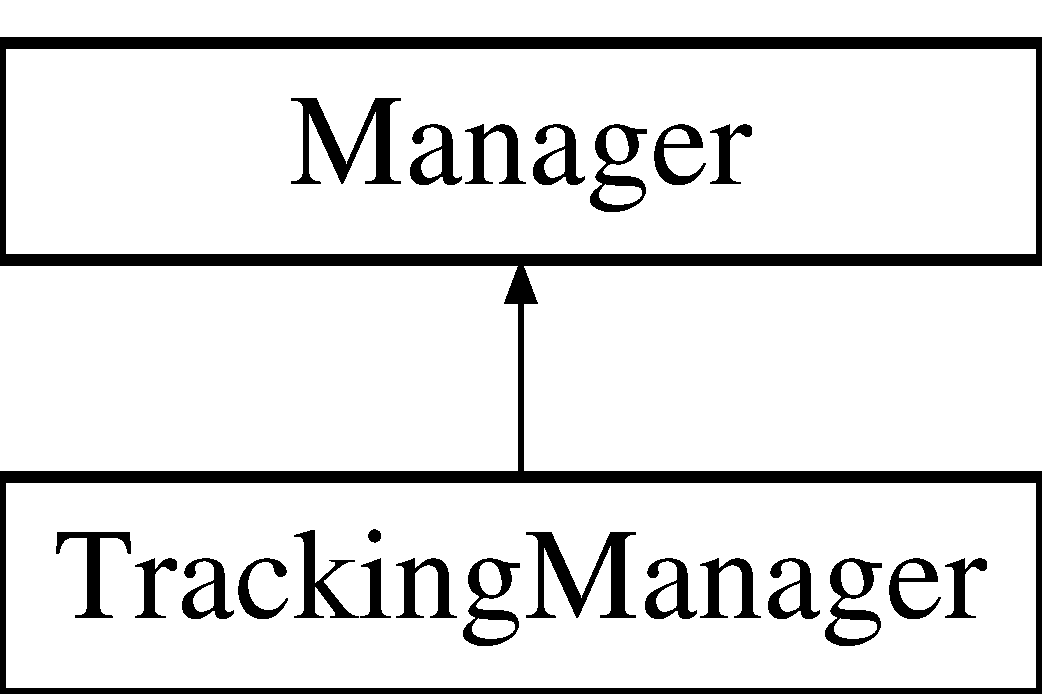
\includegraphics[height=2.000000cm]{classTrackingManager}
\end{center}
\end{figure}
\subsection*{Public Member Functions}
\begin{DoxyCompactItemize}
\item 
\hyperlink{classTrackingManager_a9fb18e3ad20bc3eb3e9e3eb2e6b5748c}{Tracking\-Manager} ()
\begin{DoxyCompactList}\small\item\em Constructor for Tracking manager. \end{DoxyCompactList}\item 
void \hyperlink{classTrackingManager_a6331ac24f748ea336db5a7303a3dce60}{manage} (\hyperlink{classActionData}{Action\-Data} \&action\-\_\-data\-\_\-container)
\begin{DoxyCompactList}\small\item\em Manage function allowing the position of all \hyperlink{classTrackable}{Trackable} entities to be kept. \end{DoxyCompactList}\item 
void \hyperlink{classTrackingManager_af0102b33b841a415bdce8605b7c0a11b}{add\-New\-Entity} (std\-::weak\-\_\-ptr$<$ \hyperlink{classTrackable}{Trackable} $>$ new\-\_\-entity)
\begin{DoxyCompactList}\small\item\em Add Trackable-\/type shared\-\_\-ptr's to the Tracking\-Managers internal data members. \end{DoxyCompactList}\item 
const float \hyperlink{classTrackingManager_ab455df1659739739b2be5f42f08e4b26}{get\-P1\-Position\-X} ()
\begin{DoxyCompactList}\small\item\em Return x position of P1 \hyperlink{classTank}{Tank}. \end{DoxyCompactList}\item 
const float \hyperlink{classTrackingManager_ab79ae59918b07ad546cd7d95cfc983f6}{get\-P1\-Position\-Y} ()
\begin{DoxyCompactList}\small\item\em Return y position of P1 \hyperlink{classTank}{Tank}. \end{DoxyCompactList}\item 
const float \hyperlink{classTrackingManager_aad99796d4377109c93177204db15d1a8}{get\-P1\-Rotation} ()
\begin{DoxyCompactList}\small\item\em Return rotation of P1 \hyperlink{classTank}{Tank}. \end{DoxyCompactList}\item 
const float \hyperlink{classTrackingManager_acb6e621ee44b3d4589fd9e5941eb210f}{get\-P2\-Position\-X} ()
\begin{DoxyCompactList}\small\item\em Return x position of P2 \hyperlink{classTank}{Tank}. \end{DoxyCompactList}\item 
const float \hyperlink{classTrackingManager_af4f90d28fce0d8930ae555a3c1fa4bb8}{get\-P2\-Position\-Y} ()
\begin{DoxyCompactList}\small\item\em Return y position of P2 \hyperlink{classTank}{Tank}. \end{DoxyCompactList}\item 
const float \hyperlink{classTrackingManager_a61bc8a3a82f0cd4064d5e2aa53677ebb}{get\-P2\-Rotation} ()
\begin{DoxyCompactList}\small\item\em Return rotation of P2 \hyperlink{classTank}{Tank}. \end{DoxyCompactList}\item 
const std\-::vector$<$ float $>$ \& \hyperlink{classTrackingManager_ab74d90eb6562d1c25a8a3abefa36d588}{get\-Turret\-Positions\-X} ()
\begin{DoxyCompactList}\small\item\em Return x position of all Turrets. \end{DoxyCompactList}\item 
const std\-::vector$<$ float $>$ \& \hyperlink{classTrackingManager_a82406f448e4cea6dc036e57b467eafaf}{get\-Turret\-Positions\-Y} ()
\begin{DoxyCompactList}\small\item\em Return y position of all Turrets. \end{DoxyCompactList}\item 
const std\-::vector$<$ float $>$ \& \hyperlink{classTrackingManager_ab073910a54a6e8badb90ae3b9e0e3cc7}{get\-Turret\-Rotations} ()
\begin{DoxyCompactList}\small\item\em Return rotation of all Turrets. \end{DoxyCompactList}\item 
virtual \hyperlink{classTrackingManager_aab0fa1e178458935019e6459d11ddea2}{$\sim$\-Tracking\-Manager} ()
\begin{DoxyCompactList}\small\item\em Destructor for Tracking manager. \end{DoxyCompactList}\end{DoxyCompactItemize}
\subsection*{Private Member Functions}
\begin{DoxyCompactItemize}
\item 
void \hyperlink{classTrackingManager_a66f8f6f788618cb5aecfc1c228be2460}{remove\-Garbage} ()
\begin{DoxyCompactList}\small\item\em Remove all deleted entities from \-\_\-trackables. \end{DoxyCompactList}\end{DoxyCompactItemize}
\subsection*{Private Attributes}
\begin{DoxyCompactItemize}
\item 
std\-::vector$<$ std\-::weak\-\_\-ptr\\*
$<$ \hyperlink{classTrackable}{Trackable} $>$ $>$ \hyperlink{classTrackingManager_add21c42cf5a993fbf5a95abd7e36f3dc}{\-\_\-trackables}
\begin{DoxyCompactList}\small\item\em Pointers to all trackable entities within the game world. \end{DoxyCompactList}\item 
\hyperlink{classGeometryEngine}{Geometry\-Engine} \hyperlink{classTrackingManager_a9bf3e308977ec91b61c7bf5d269f35dd}{\-\_\-geometry\-\_\-engine}
\begin{DoxyCompactList}\small\item\em Helper Engine. \end{DoxyCompactList}\item 
float \hyperlink{classTrackingManager_a8c7de22662c27124fac80902d4f8ba41}{\-\_\-p1\-Rotation}
\begin{DoxyCompactList}\small\item\em Player 1 tank current rotation. \end{DoxyCompactList}\item 
float \hyperlink{classTrackingManager_a14b43a5e0cd605fff6b3308d0377f697}{\-\_\-p1\-Position\-X}
\begin{DoxyCompactList}\small\item\em Player 1 tank current x position. \end{DoxyCompactList}\item 
float \hyperlink{classTrackingManager_aa5b384a370b1ddccf76badc8a55459b1}{\-\_\-p1\-Position\-Y}
\begin{DoxyCompactList}\small\item\em Player 1 tank current y position. \end{DoxyCompactList}\item 
\hyperlink{structrect__corners}{rect\-\_\-corners} \hyperlink{classTrackingManager_a4916085aebb34a3921f3592d7ae07767}{\-\_\-p1\-Bounding\-Box}
\begin{DoxyCompactList}\small\item\em Player 1 Bounding box. \end{DoxyCompactList}\item 
float \hyperlink{classTrackingManager_a04442a7d5e399370637c9e334a257eb6}{\-\_\-p2\-Rotation}
\begin{DoxyCompactList}\small\item\em Player 2 tank current rotation. \end{DoxyCompactList}\item 
float \hyperlink{classTrackingManager_a0f3a043190aba11b137c52052dc2ed3a}{\-\_\-p2\-Position\-X}
\begin{DoxyCompactList}\small\item\em Player 2tank current x position. \end{DoxyCompactList}\item 
float \hyperlink{classTrackingManager_ad4d803802447b6c8a1a09104263fd829}{\-\_\-p2\-Position\-Y}
\begin{DoxyCompactList}\small\item\em Player 2 tank current y position. \end{DoxyCompactList}\item 
\hyperlink{structrect__corners}{rect\-\_\-corners} \hyperlink{classTrackingManager_a345399f12e52bc4b23786fe73b26a6ff}{\-\_\-p2\-Bounding\-Box}
\begin{DoxyCompactList}\small\item\em Player 2 Bounding box. \end{DoxyCompactList}\item 
std\-::vector$<$ float $>$ \hyperlink{classTrackingManager_ad66641438bdcf33e772ef4ec1cdc7e14}{\-\_\-turret\-Positions\-X}
\begin{DoxyCompactList}\small\item\em All of the Turrets current x positions. \end{DoxyCompactList}\item 
std\-::vector$<$ float $>$ \hyperlink{classTrackingManager_aaf2aa5d29aa7a7abd3a7e7f27bff7340}{\-\_\-turret\-Positions\-Y}
\begin{DoxyCompactList}\small\item\em All of the Turrets current y positions. \end{DoxyCompactList}\item 
std\-::vector$<$ float $>$ \hyperlink{classTrackingManager_adce9702d80c3554e7a359a145a6d2632}{\-\_\-turret\-Rotations}
\begin{DoxyCompactList}\small\item\em all of the Turrets current Rotations \end{DoxyCompactList}\end{DoxyCompactItemize}


\subsection{Detailed Description}
\hyperlink{classManager}{Manager} responsible for keeping track of game entity positions. 

Definition at line 22 of file Tracking\-Manager.\-h.



\subsection{Constructor \& Destructor Documentation}
\hypertarget{classTrackingManager_a9fb18e3ad20bc3eb3e9e3eb2e6b5748c}{\index{Tracking\-Manager@{Tracking\-Manager}!Tracking\-Manager@{Tracking\-Manager}}
\index{Tracking\-Manager@{Tracking\-Manager}!TrackingManager@{Tracking\-Manager}}
\subsubsection[{Tracking\-Manager}]{\setlength{\rightskip}{0pt plus 5cm}Tracking\-Manager\-::\-Tracking\-Manager (
\begin{DoxyParamCaption}
{}
\end{DoxyParamCaption}
)}}\label{classTrackingManager_a9fb18e3ad20bc3eb3e9e3eb2e6b5748c}


Constructor for Tracking manager. 

Constructor that initialises the \-\_\-geometry\-\_\-engine. 

Definition at line 15 of file Tracking\-Manager.\-cpp.


\begin{DoxyCode}
15                                 :
16     \hyperlink{classTrackingManager_a9bf3e308977ec91b61c7bf5d269f35dd}{\_geometry\_engine}()
17 \{
18 
19 \}
\end{DoxyCode}
\hypertarget{classTrackingManager_aab0fa1e178458935019e6459d11ddea2}{\index{Tracking\-Manager@{Tracking\-Manager}!$\sim$\-Tracking\-Manager@{$\sim$\-Tracking\-Manager}}
\index{$\sim$\-Tracking\-Manager@{$\sim$\-Tracking\-Manager}!TrackingManager@{Tracking\-Manager}}
\subsubsection[{$\sim$\-Tracking\-Manager}]{\setlength{\rightskip}{0pt plus 5cm}Tracking\-Manager\-::$\sim$\-Tracking\-Manager (
\begin{DoxyParamCaption}
{}
\end{DoxyParamCaption}
)\hspace{0.3cm}{\ttfamily [virtual]}}}\label{classTrackingManager_aab0fa1e178458935019e6459d11ddea2}


Destructor for Tracking manager. 



Definition at line 21 of file Tracking\-Manager.\-cpp.


\begin{DoxyCode}
22 \{
23 
24 \}
\end{DoxyCode}


\subsection{Member Function Documentation}
\hypertarget{classTrackingManager_af0102b33b841a415bdce8605b7c0a11b}{\index{Tracking\-Manager@{Tracking\-Manager}!add\-New\-Entity@{add\-New\-Entity}}
\index{add\-New\-Entity@{add\-New\-Entity}!TrackingManager@{Tracking\-Manager}}
\subsubsection[{add\-New\-Entity}]{\setlength{\rightskip}{0pt plus 5cm}void Tracking\-Manager\-::add\-New\-Entity (
\begin{DoxyParamCaption}
\item[{std\-::weak\-\_\-ptr$<$ {\bf Trackable} $>$}]{new\-\_\-entity}
\end{DoxyParamCaption}
)}}\label{classTrackingManager_af0102b33b841a415bdce8605b7c0a11b}


Add Trackable-\/type shared\-\_\-ptr's to the Tracking\-Managers internal data members. 



Definition at line 196 of file Tracking\-Manager.\-cpp.



References \-\_\-trackables.



Referenced by Game\-::add\-Trackable(), and T\-E\-S\-T().


\begin{DoxyCode}
197 \{
198     \hyperlink{classTrackingManager_add21c42cf5a993fbf5a95abd7e36f3dc}{\_trackables}.push\_back(new\_entity);
199 \}
\end{DoxyCode}
\hypertarget{classTrackingManager_ab455df1659739739b2be5f42f08e4b26}{\index{Tracking\-Manager@{Tracking\-Manager}!get\-P1\-Position\-X@{get\-P1\-Position\-X}}
\index{get\-P1\-Position\-X@{get\-P1\-Position\-X}!TrackingManager@{Tracking\-Manager}}
\subsubsection[{get\-P1\-Position\-X}]{\setlength{\rightskip}{0pt plus 5cm}const float Tracking\-Manager\-::get\-P1\-Position\-X (
\begin{DoxyParamCaption}
{}
\end{DoxyParamCaption}
)}}\label{classTrackingManager_ab455df1659739739b2be5f42f08e4b26}


Return x position of P1 \hyperlink{classTank}{Tank}. 



Definition at line 147 of file Tracking\-Manager.\-cpp.



References \-\_\-p1\-Position\-X.



Referenced by Game\-::add\-New\-World\-Entity(), and T\-E\-S\-T().


\begin{DoxyCode}
148 \{
149     \textcolor{keywordflow}{return} \hyperlink{classTrackingManager_a14b43a5e0cd605fff6b3308d0377f697}{\_p1PositionX};
150 \}
\end{DoxyCode}
\hypertarget{classTrackingManager_ab79ae59918b07ad546cd7d95cfc983f6}{\index{Tracking\-Manager@{Tracking\-Manager}!get\-P1\-Position\-Y@{get\-P1\-Position\-Y}}
\index{get\-P1\-Position\-Y@{get\-P1\-Position\-Y}!TrackingManager@{Tracking\-Manager}}
\subsubsection[{get\-P1\-Position\-Y}]{\setlength{\rightskip}{0pt plus 5cm}const float Tracking\-Manager\-::get\-P1\-Position\-Y (
\begin{DoxyParamCaption}
{}
\end{DoxyParamCaption}
)}}\label{classTrackingManager_ab79ae59918b07ad546cd7d95cfc983f6}


Return y position of P1 \hyperlink{classTank}{Tank}. 



Definition at line 155 of file Tracking\-Manager.\-cpp.



References \-\_\-p1\-Position\-Y.



Referenced by Game\-::add\-New\-World\-Entity(), and T\-E\-S\-T().


\begin{DoxyCode}
156 \{
157     \textcolor{keywordflow}{return} \hyperlink{classTrackingManager_aa5b384a370b1ddccf76badc8a55459b1}{\_p1PositionY};
158 \}
\end{DoxyCode}
\hypertarget{classTrackingManager_aad99796d4377109c93177204db15d1a8}{\index{Tracking\-Manager@{Tracking\-Manager}!get\-P1\-Rotation@{get\-P1\-Rotation}}
\index{get\-P1\-Rotation@{get\-P1\-Rotation}!TrackingManager@{Tracking\-Manager}}
\subsubsection[{get\-P1\-Rotation}]{\setlength{\rightskip}{0pt plus 5cm}const float Tracking\-Manager\-::get\-P1\-Rotation (
\begin{DoxyParamCaption}
{}
\end{DoxyParamCaption}
)}}\label{classTrackingManager_aad99796d4377109c93177204db15d1a8}


Return rotation of P1 \hyperlink{classTank}{Tank}. 



Definition at line 164 of file Tracking\-Manager.\-cpp.



References \-\_\-p1\-Rotation.



Referenced by Game\-::add\-New\-World\-Entity(), and T\-E\-S\-T().


\begin{DoxyCode}
165 \{
166     \textcolor{keywordflow}{return} \hyperlink{classTrackingManager_a8c7de22662c27124fac80902d4f8ba41}{\_p1Rotation};
167 \}
\end{DoxyCode}
\hypertarget{classTrackingManager_acb6e621ee44b3d4589fd9e5941eb210f}{\index{Tracking\-Manager@{Tracking\-Manager}!get\-P2\-Position\-X@{get\-P2\-Position\-X}}
\index{get\-P2\-Position\-X@{get\-P2\-Position\-X}!TrackingManager@{Tracking\-Manager}}
\subsubsection[{get\-P2\-Position\-X}]{\setlength{\rightskip}{0pt plus 5cm}const float Tracking\-Manager\-::get\-P2\-Position\-X (
\begin{DoxyParamCaption}
{}
\end{DoxyParamCaption}
)}}\label{classTrackingManager_acb6e621ee44b3d4589fd9e5941eb210f}


Return x position of P2 \hyperlink{classTank}{Tank}. 



Definition at line 172 of file Tracking\-Manager.\-cpp.



References \-\_\-p2\-Position\-X.



Referenced by Game\-::add\-New\-World\-Entity(), and T\-E\-S\-T().


\begin{DoxyCode}
173 \{
174     \textcolor{keywordflow}{return} \hyperlink{classTrackingManager_a0f3a043190aba11b137c52052dc2ed3a}{\_p2PositionX};
175 \}
\end{DoxyCode}
\hypertarget{classTrackingManager_af4f90d28fce0d8930ae555a3c1fa4bb8}{\index{Tracking\-Manager@{Tracking\-Manager}!get\-P2\-Position\-Y@{get\-P2\-Position\-Y}}
\index{get\-P2\-Position\-Y@{get\-P2\-Position\-Y}!TrackingManager@{Tracking\-Manager}}
\subsubsection[{get\-P2\-Position\-Y}]{\setlength{\rightskip}{0pt plus 5cm}const float Tracking\-Manager\-::get\-P2\-Position\-Y (
\begin{DoxyParamCaption}
{}
\end{DoxyParamCaption}
)}}\label{classTrackingManager_af4f90d28fce0d8930ae555a3c1fa4bb8}


Return y position of P2 \hyperlink{classTank}{Tank}. 



Definition at line 180 of file Tracking\-Manager.\-cpp.



References \-\_\-p2\-Position\-Y.



Referenced by Game\-::add\-New\-World\-Entity(), and T\-E\-S\-T().


\begin{DoxyCode}
181 \{
182     \textcolor{keywordflow}{return} \hyperlink{classTrackingManager_ad4d803802447b6c8a1a09104263fd829}{\_p2PositionY};
183 \}
\end{DoxyCode}
\hypertarget{classTrackingManager_a61bc8a3a82f0cd4064d5e2aa53677ebb}{\index{Tracking\-Manager@{Tracking\-Manager}!get\-P2\-Rotation@{get\-P2\-Rotation}}
\index{get\-P2\-Rotation@{get\-P2\-Rotation}!TrackingManager@{Tracking\-Manager}}
\subsubsection[{get\-P2\-Rotation}]{\setlength{\rightskip}{0pt plus 5cm}const float Tracking\-Manager\-::get\-P2\-Rotation (
\begin{DoxyParamCaption}
{}
\end{DoxyParamCaption}
)}}\label{classTrackingManager_a61bc8a3a82f0cd4064d5e2aa53677ebb}


Return rotation of P2 \hyperlink{classTank}{Tank}. 



Definition at line 188 of file Tracking\-Manager.\-cpp.



References \-\_\-p2\-Rotation.



Referenced by Game\-::add\-New\-World\-Entity(), and T\-E\-S\-T().


\begin{DoxyCode}
189 \{
190     \textcolor{keywordflow}{return} \hyperlink{classTrackingManager_a04442a7d5e399370637c9e334a257eb6}{\_p2Rotation};
191 \}
\end{DoxyCode}
\hypertarget{classTrackingManager_ab74d90eb6562d1c25a8a3abefa36d588}{\index{Tracking\-Manager@{Tracking\-Manager}!get\-Turret\-Positions\-X@{get\-Turret\-Positions\-X}}
\index{get\-Turret\-Positions\-X@{get\-Turret\-Positions\-X}!TrackingManager@{Tracking\-Manager}}
\subsubsection[{get\-Turret\-Positions\-X}]{\setlength{\rightskip}{0pt plus 5cm}const std\-::vector$<$ float $>$ \& Tracking\-Manager\-::get\-Turret\-Positions\-X (
\begin{DoxyParamCaption}
{}
\end{DoxyParamCaption}
)}}\label{classTrackingManager_ab74d90eb6562d1c25a8a3abefa36d588}


Return x position of all Turrets. 



Definition at line 122 of file Tracking\-Manager.\-cpp.



References \-\_\-turret\-Positions\-X.



Referenced by Game\-::add\-New\-World\-Entity(), and T\-E\-S\-T().


\begin{DoxyCode}
123 \{
124     \textcolor{keywordflow}{return} \hyperlink{classTrackingManager_ad66641438bdcf33e772ef4ec1cdc7e14}{\_turretPositionsX};
125 \}
\end{DoxyCode}
\hypertarget{classTrackingManager_a82406f448e4cea6dc036e57b467eafaf}{\index{Tracking\-Manager@{Tracking\-Manager}!get\-Turret\-Positions\-Y@{get\-Turret\-Positions\-Y}}
\index{get\-Turret\-Positions\-Y@{get\-Turret\-Positions\-Y}!TrackingManager@{Tracking\-Manager}}
\subsubsection[{get\-Turret\-Positions\-Y}]{\setlength{\rightskip}{0pt plus 5cm}const std\-::vector$<$ float $>$ \& Tracking\-Manager\-::get\-Turret\-Positions\-Y (
\begin{DoxyParamCaption}
{}
\end{DoxyParamCaption}
)}}\label{classTrackingManager_a82406f448e4cea6dc036e57b467eafaf}


Return y position of all Turrets. 



Definition at line 131 of file Tracking\-Manager.\-cpp.



References \-\_\-turret\-Positions\-Y.



Referenced by Game\-::add\-New\-World\-Entity(), and T\-E\-S\-T().


\begin{DoxyCode}
132 \{
133     \textcolor{keywordflow}{return} \hyperlink{classTrackingManager_aaf2aa5d29aa7a7abd3a7e7f27bff7340}{\_turretPositionsY};
134 \}
\end{DoxyCode}
\hypertarget{classTrackingManager_ab073910a54a6e8badb90ae3b9e0e3cc7}{\index{Tracking\-Manager@{Tracking\-Manager}!get\-Turret\-Rotations@{get\-Turret\-Rotations}}
\index{get\-Turret\-Rotations@{get\-Turret\-Rotations}!TrackingManager@{Tracking\-Manager}}
\subsubsection[{get\-Turret\-Rotations}]{\setlength{\rightskip}{0pt plus 5cm}const std\-::vector$<$ float $>$ \& Tracking\-Manager\-::get\-Turret\-Rotations (
\begin{DoxyParamCaption}
{}
\end{DoxyParamCaption}
)}}\label{classTrackingManager_ab073910a54a6e8badb90ae3b9e0e3cc7}


Return rotation of all Turrets. 



Definition at line 139 of file Tracking\-Manager.\-cpp.



References \-\_\-turret\-Rotations.



Referenced by Game\-::add\-New\-World\-Entity().


\begin{DoxyCode}
140 \{
141     \textcolor{keywordflow}{return} \hyperlink{classTrackingManager_adce9702d80c3554e7a359a145a6d2632}{\_turretRotations};
142 \}
\end{DoxyCode}
\hypertarget{classTrackingManager_a6331ac24f748ea336db5a7303a3dce60}{\index{Tracking\-Manager@{Tracking\-Manager}!manage@{manage}}
\index{manage@{manage}!TrackingManager@{Tracking\-Manager}}
\subsubsection[{manage}]{\setlength{\rightskip}{0pt plus 5cm}void Tracking\-Manager\-::manage (
\begin{DoxyParamCaption}
\item[{{\bf Action\-Data} \&}]{action\-\_\-data\-\_\-container}
\end{DoxyParamCaption}
)}}\label{classTrackingManager_a6331ac24f748ea336db5a7303a3dce60}


Manage function allowing the position of all \hyperlink{classTrackable}{Trackable} entities to be kept. 

This includes the tracking of the tanks by the turrets. The positions are obtained and then passed to the \-\_\-geometry\-\_\-engine where comparisons are made. 
\begin{DoxyParams}{Parameters}
{\em action\-\_\-data\-\_\-container} & \-:\-: Will set turret file in this container if needs be \\
\hline
\end{DoxyParams}


Definition at line 31 of file Tracking\-Manager.\-cpp.



References \-\_\-geometry\-\_\-engine, \-\_\-p1\-Bounding\-Box, \-\_\-p1\-Position\-X, \-\_\-p1\-Position\-Y, \-\_\-p1\-Rotation, \-\_\-p2\-Bounding\-Box, \-\_\-p2\-Position\-X, \-\_\-p2\-Position\-Y, \-\_\-p2\-Rotation, \-\_\-trackables, \-\_\-turret\-Positions\-X, \-\_\-turret\-Positions\-Y, \-\_\-turret\-Rotations, Geometry\-Engine\-::calculate\-Vector\-Length(), Geometry\-Engine\-::is\-In\-Line\-Of\-Fire(), p1\-\_\-tank, p2\-\_\-tank, remove\-Garbage(), Action\-Data\-::set\-Turret\-Fire(), and turret.



Referenced by Game\-::run\-All\-Managers(), and T\-E\-S\-T().


\begin{DoxyCode}
32 \{
33     \hyperlink{classTrackingManager_a66f8f6f788618cb5aecfc1c228be2460}{removeGarbage}();
34     \textcolor{comment}{//Clear position vectors for new cycle}
35     \hyperlink{classTrackingManager_ad66641438bdcf33e772ef4ec1cdc7e14}{\_turretPositionsX}.clear();
36     \hyperlink{classTrackingManager_aaf2aa5d29aa7a7abd3a7e7f27bff7340}{\_turretPositionsY}.clear();
37     \hyperlink{classTrackingManager_adce9702d80c3554e7a359a145a6d2632}{\_turretRotations}.clear();
38 
39     \textcolor{keyword}{auto} \_trackables\_itterator = \hyperlink{classTrackingManager_add21c42cf5a993fbf5a95abd7e36f3dc}{\_trackables}.begin();
40     \textcolor{keywordflow}{for}(; \_trackables\_itterator != \hyperlink{classTrackingManager_add21c42cf5a993fbf5a95abd7e36f3dc}{\_trackables}.end(); \_trackables\_itterator++)
41     \{
42         \textcolor{comment}{//Convert Itterator to Weak Pointer}
43         std::weak\_ptr<Trackable> entity\_track\_wp = (*\_trackables\_itterator);
44         \textcolor{comment}{//Convert Weak Pointer to Shared Pointer}
45         std::shared\_ptr<Trackable> entity\_track\_sp = entity\_track\_wp.lock();
46         \textcolor{comment}{//Check to see if entity still exists}
47 
48             \textcolor{keywordflow}{if}(entity\_track\_sp->getType() == \hyperlink{Structures_8h_a6d8f83e710b27d4f86c45f0bb77066e3a31fa78b2b7dd774f5158a16ef230932e}{p1\_tank})
49             \{
50                 \hyperlink{classTrackingManager_a14b43a5e0cd605fff6b3308d0377f697}{\_p1PositionX} = entity\_track\_sp->getPositionX();
51                 \hyperlink{classTrackingManager_aa5b384a370b1ddccf76badc8a55459b1}{\_p1PositionY} = entity\_track\_sp->getPositionY();
52                 \hyperlink{classTrackingManager_a8c7de22662c27124fac80902d4f8ba41}{\_p1Rotation} = entity\_track\_sp->getOrientation();
53                 \hyperlink{classTrackingManager_a4916085aebb34a3921f3592d7ae07767}{\_p1BoundingBox} = entity\_track\_sp->getTrackingBoundingBox();
54             \}
55 
56             \textcolor{keywordflow}{else} \textcolor{keywordflow}{if}(entity\_track\_sp->getType() == \hyperlink{Structures_8h_a6d8f83e710b27d4f86c45f0bb77066e3a3d48d62c7b88e7ee171698fe56dc9e59}{p2\_tank})
57             \{
58                 \hyperlink{classTrackingManager_a0f3a043190aba11b137c52052dc2ed3a}{\_p2PositionX} = entity\_track\_sp->getPositionX();
59                 \hyperlink{classTrackingManager_ad4d803802447b6c8a1a09104263fd829}{\_p2PositionY} = entity\_track\_sp->getPositionY();
60                 \hyperlink{classTrackingManager_a04442a7d5e399370637c9e334a257eb6}{\_p2Rotation} = entity\_track\_sp->getOrientation();
61                 \hyperlink{classTrackingManager_a345399f12e52bc4b23786fe73b26a6ff}{\_p2BoundingBox} = entity\_track\_sp->getTrackingBoundingBox();
62             \}
63 
64             \textcolor{keywordflow}{else} \textcolor{keywordflow}{if}(entity\_track\_sp->getType() == \hyperlink{Structures_8h_a6d8f83e710b27d4f86c45f0bb77066e3a85c730ac9ffc13ac94e6e860579928a1}{turret})
65             \{
66                 \textcolor{comment}{//Temp variables}
67                 \textcolor{keywordtype}{float} temp\_Turret\_Xpos = entity\_track\_sp->getPositionX();
68                 \textcolor{keywordtype}{float} temp\_Turret\_Ypos = entity\_track\_sp->getPositionY();
69                 \textcolor{keywordtype}{float} temp\_Turret\_Rotation = entity\_track\_sp->getOrientation();
70                 \textcolor{keyword}{auto} temp\_Turret\_BoundingBox = entity\_track\_sp->getTrackingBoundingBox();
71 
72                 \textcolor{comment}{//See if turrets are viewing (tank1 or tank2) and it is in proximity}
73                 \textcolor{comment}{//Using case gaurds}
74                 \textcolor{keywordflow}{if}((\hyperlink{classTrackingManager_a9bf3e308977ec91b61c7bf5d269f35dd}{\_geometry\_engine}.\hyperlink{classGeometryEngine_af21c9c2e172169130af88fa6f3aa5fe7}{isInLineOfFire}(temp\_Turret\_Rotation, 
      temp\_Turret\_BoundingBox, \hyperlink{classTrackingManager_a4916085aebb34a3921f3592d7ae07767}{\_p1BoundingBox}, temp\_Turret\_Ypos, 
      \hyperlink{classTrackingManager_aa5b384a370b1ddccf76badc8a55459b1}{\_p1PositionY})) &&
75                    (\hyperlink{classTrackingManager_a9bf3e308977ec91b61c7bf5d269f35dd}{\_geometry\_engine}.\hyperlink{classGeometryEngine_a99634c40d20ab72ab30289a6ff4abe39}{calculateVectorLength}(
      temp\_Turret\_Xpos,temp\_Turret\_Ypos,\hyperlink{classTrackingManager_a14b43a5e0cd605fff6b3308d0377f697}{\_p1PositionX},\hyperlink{classTrackingManager_ad4d803802447b6c8a1a09104263fd829}{\_p2PositionY}) < 400.0))
76                 \{
77                     action\_data\_container.\hyperlink{classActionData_a30502665240f4a0b0e37fbcd6447b590}{setTurretFire}();
78                     \hyperlink{classTrackingManager_ad66641438bdcf33e772ef4ec1cdc7e14}{\_turretPositionsX}.push\_back(temp\_Turret\_Xpos);
79                     \hyperlink{classTrackingManager_aaf2aa5d29aa7a7abd3a7e7f27bff7340}{\_turretPositionsY}.push\_back(temp\_Turret\_Ypos);
80                     \hyperlink{classTrackingManager_adce9702d80c3554e7a359a145a6d2632}{\_turretRotations}.push\_back(temp\_Turret\_Rotation);
81                 \}
82 
83                 \textcolor{keywordflow}{if}((\hyperlink{classTrackingManager_a9bf3e308977ec91b61c7bf5d269f35dd}{\_geometry\_engine}.\hyperlink{classGeometryEngine_af21c9c2e172169130af88fa6f3aa5fe7}{isInLineOfFire}(temp\_Turret\_Rotation, 
      temp\_Turret\_BoundingBox, \hyperlink{classTrackingManager_a345399f12e52bc4b23786fe73b26a6ff}{\_p2BoundingBox}, temp\_Turret\_Ypos, 
      \hyperlink{classTrackingManager_ad4d803802447b6c8a1a09104263fd829}{\_p2PositionY})) &&
84                    (\hyperlink{classTrackingManager_a9bf3e308977ec91b61c7bf5d269f35dd}{\_geometry\_engine}.\hyperlink{classGeometryEngine_a99634c40d20ab72ab30289a6ff4abe39}{calculateVectorLength}(
      temp\_Turret\_Xpos,temp\_Turret\_Ypos,\hyperlink{classTrackingManager_a0f3a043190aba11b137c52052dc2ed3a}{\_p2PositionX},\hyperlink{classTrackingManager_ad4d803802447b6c8a1a09104263fd829}{\_p2PositionY}) < 400.0))
85                 \{
86                     action\_data\_container.\hyperlink{classActionData_a30502665240f4a0b0e37fbcd6447b590}{setTurretFire}();
87                     \hyperlink{classTrackingManager_ad66641438bdcf33e772ef4ec1cdc7e14}{\_turretPositionsX}.push\_back(temp\_Turret\_Xpos);
88                     \hyperlink{classTrackingManager_aaf2aa5d29aa7a7abd3a7e7f27bff7340}{\_turretPositionsY}.push\_back(temp\_Turret\_Ypos);
89                     \hyperlink{classTrackingManager_adce9702d80c3554e7a359a145a6d2632}{\_turretRotations}.push\_back(temp\_Turret\_Rotation);
90                 \}
91             \}
92     \}\textcolor{comment}{//For}
93 \}\textcolor{comment}{//function}
\end{DoxyCode}
\hypertarget{classTrackingManager_a66f8f6f788618cb5aecfc1c228be2460}{\index{Tracking\-Manager@{Tracking\-Manager}!remove\-Garbage@{remove\-Garbage}}
\index{remove\-Garbage@{remove\-Garbage}!TrackingManager@{Tracking\-Manager}}
\subsubsection[{remove\-Garbage}]{\setlength{\rightskip}{0pt plus 5cm}void Tracking\-Manager\-::remove\-Garbage (
\begin{DoxyParamCaption}
{}
\end{DoxyParamCaption}
)\hspace{0.3cm}{\ttfamily [private]}}}\label{classTrackingManager_a66f8f6f788618cb5aecfc1c228be2460}


Remove all deleted entities from \-\_\-trackables. 

Clear all deleted pointers. 

Definition at line 98 of file Tracking\-Manager.\-cpp.



References \-\_\-trackables.



Referenced by manage().


\begin{DoxyCode}
99 \{
100     \textcolor{comment}{//Clear all deleted entities from the \_trackables vector}
101     \textcolor{keyword}{auto} removal = \hyperlink{classTrackingManager_add21c42cf5a993fbf5a95abd7e36f3dc}{\_trackables}.begin();
102     \textcolor{keywordflow}{for} (; removal != \hyperlink{classTrackingManager_add21c42cf5a993fbf5a95abd7e36f3dc}{\_trackables}.end();)
103     \{
104         std::weak\_ptr<Trackable> removal\_wp = (*removal);
105         \textcolor{comment}{//Convert weak\_ptr to shared\_ptr}
106         std::shared\_ptr<Trackable> removal\_sp = removal\_wp.lock();
107         \textcolor{comment}{//Test if pointer still valid}
108         \textcolor{keywordflow}{if}(removal\_sp)
109         \{
110             removal++;
111         \}
112         \textcolor{keywordflow}{else}
113         \{
114             \hyperlink{classTrackingManager_add21c42cf5a993fbf5a95abd7e36f3dc}{\_trackables}.erase(removal);
115         \}
116     \}\textcolor{comment}{// if}
117 \}\textcolor{comment}{//function}
\end{DoxyCode}


\subsection{Member Data Documentation}
\hypertarget{classTrackingManager_a9bf3e308977ec91b61c7bf5d269f35dd}{\index{Tracking\-Manager@{Tracking\-Manager}!\-\_\-geometry\-\_\-engine@{\-\_\-geometry\-\_\-engine}}
\index{\-\_\-geometry\-\_\-engine@{\-\_\-geometry\-\_\-engine}!TrackingManager@{Tracking\-Manager}}
\subsubsection[{\-\_\-geometry\-\_\-engine}]{\setlength{\rightskip}{0pt plus 5cm}{\bf Geometry\-Engine} Tracking\-Manager\-::\-\_\-geometry\-\_\-engine\hspace{0.3cm}{\ttfamily [private]}}}\label{classTrackingManager_a9bf3e308977ec91b61c7bf5d269f35dd}


Helper Engine. 



Definition at line 63 of file Tracking\-Manager.\-h.



Referenced by manage().

\hypertarget{classTrackingManager_a4916085aebb34a3921f3592d7ae07767}{\index{Tracking\-Manager@{Tracking\-Manager}!\-\_\-p1\-Bounding\-Box@{\-\_\-p1\-Bounding\-Box}}
\index{\-\_\-p1\-Bounding\-Box@{\-\_\-p1\-Bounding\-Box}!TrackingManager@{Tracking\-Manager}}
\subsubsection[{\-\_\-p1\-Bounding\-Box}]{\setlength{\rightskip}{0pt plus 5cm}{\bf rect\-\_\-corners} Tracking\-Manager\-::\-\_\-p1\-Bounding\-Box\hspace{0.3cm}{\ttfamily [private]}}}\label{classTrackingManager_a4916085aebb34a3921f3592d7ae07767}


Player 1 Bounding box. 



Definition at line 72 of file Tracking\-Manager.\-h.



Referenced by manage().

\hypertarget{classTrackingManager_a14b43a5e0cd605fff6b3308d0377f697}{\index{Tracking\-Manager@{Tracking\-Manager}!\-\_\-p1\-Position\-X@{\-\_\-p1\-Position\-X}}
\index{\-\_\-p1\-Position\-X@{\-\_\-p1\-Position\-X}!TrackingManager@{Tracking\-Manager}}
\subsubsection[{\-\_\-p1\-Position\-X}]{\setlength{\rightskip}{0pt plus 5cm}float Tracking\-Manager\-::\-\_\-p1\-Position\-X\hspace{0.3cm}{\ttfamily [private]}}}\label{classTrackingManager_a14b43a5e0cd605fff6b3308d0377f697}


Player 1 tank current x position. 



Definition at line 68 of file Tracking\-Manager.\-h.



Referenced by get\-P1\-Position\-X(), and manage().

\hypertarget{classTrackingManager_aa5b384a370b1ddccf76badc8a55459b1}{\index{Tracking\-Manager@{Tracking\-Manager}!\-\_\-p1\-Position\-Y@{\-\_\-p1\-Position\-Y}}
\index{\-\_\-p1\-Position\-Y@{\-\_\-p1\-Position\-Y}!TrackingManager@{Tracking\-Manager}}
\subsubsection[{\-\_\-p1\-Position\-Y}]{\setlength{\rightskip}{0pt plus 5cm}float Tracking\-Manager\-::\-\_\-p1\-Position\-Y\hspace{0.3cm}{\ttfamily [private]}}}\label{classTrackingManager_aa5b384a370b1ddccf76badc8a55459b1}


Player 1 tank current y position. 



Definition at line 70 of file Tracking\-Manager.\-h.



Referenced by get\-P1\-Position\-Y(), and manage().

\hypertarget{classTrackingManager_a8c7de22662c27124fac80902d4f8ba41}{\index{Tracking\-Manager@{Tracking\-Manager}!\-\_\-p1\-Rotation@{\-\_\-p1\-Rotation}}
\index{\-\_\-p1\-Rotation@{\-\_\-p1\-Rotation}!TrackingManager@{Tracking\-Manager}}
\subsubsection[{\-\_\-p1\-Rotation}]{\setlength{\rightskip}{0pt plus 5cm}float Tracking\-Manager\-::\-\_\-p1\-Rotation\hspace{0.3cm}{\ttfamily [private]}}}\label{classTrackingManager_a8c7de22662c27124fac80902d4f8ba41}


Player 1 tank current rotation. 



Definition at line 66 of file Tracking\-Manager.\-h.



Referenced by get\-P1\-Rotation(), and manage().

\hypertarget{classTrackingManager_a345399f12e52bc4b23786fe73b26a6ff}{\index{Tracking\-Manager@{Tracking\-Manager}!\-\_\-p2\-Bounding\-Box@{\-\_\-p2\-Bounding\-Box}}
\index{\-\_\-p2\-Bounding\-Box@{\-\_\-p2\-Bounding\-Box}!TrackingManager@{Tracking\-Manager}}
\subsubsection[{\-\_\-p2\-Bounding\-Box}]{\setlength{\rightskip}{0pt plus 5cm}{\bf rect\-\_\-corners} Tracking\-Manager\-::\-\_\-p2\-Bounding\-Box\hspace{0.3cm}{\ttfamily [private]}}}\label{classTrackingManager_a345399f12e52bc4b23786fe73b26a6ff}


Player 2 Bounding box. 



Definition at line 81 of file Tracking\-Manager.\-h.



Referenced by manage().

\hypertarget{classTrackingManager_a0f3a043190aba11b137c52052dc2ed3a}{\index{Tracking\-Manager@{Tracking\-Manager}!\-\_\-p2\-Position\-X@{\-\_\-p2\-Position\-X}}
\index{\-\_\-p2\-Position\-X@{\-\_\-p2\-Position\-X}!TrackingManager@{Tracking\-Manager}}
\subsubsection[{\-\_\-p2\-Position\-X}]{\setlength{\rightskip}{0pt plus 5cm}float Tracking\-Manager\-::\-\_\-p2\-Position\-X\hspace{0.3cm}{\ttfamily [private]}}}\label{classTrackingManager_a0f3a043190aba11b137c52052dc2ed3a}


Player 2tank current x position. 



Definition at line 77 of file Tracking\-Manager.\-h.



Referenced by get\-P2\-Position\-X(), and manage().

\hypertarget{classTrackingManager_ad4d803802447b6c8a1a09104263fd829}{\index{Tracking\-Manager@{Tracking\-Manager}!\-\_\-p2\-Position\-Y@{\-\_\-p2\-Position\-Y}}
\index{\-\_\-p2\-Position\-Y@{\-\_\-p2\-Position\-Y}!TrackingManager@{Tracking\-Manager}}
\subsubsection[{\-\_\-p2\-Position\-Y}]{\setlength{\rightskip}{0pt plus 5cm}float Tracking\-Manager\-::\-\_\-p2\-Position\-Y\hspace{0.3cm}{\ttfamily [private]}}}\label{classTrackingManager_ad4d803802447b6c8a1a09104263fd829}


Player 2 tank current y position. 



Definition at line 79 of file Tracking\-Manager.\-h.



Referenced by get\-P2\-Position\-Y(), and manage().

\hypertarget{classTrackingManager_a04442a7d5e399370637c9e334a257eb6}{\index{Tracking\-Manager@{Tracking\-Manager}!\-\_\-p2\-Rotation@{\-\_\-p2\-Rotation}}
\index{\-\_\-p2\-Rotation@{\-\_\-p2\-Rotation}!TrackingManager@{Tracking\-Manager}}
\subsubsection[{\-\_\-p2\-Rotation}]{\setlength{\rightskip}{0pt plus 5cm}float Tracking\-Manager\-::\-\_\-p2\-Rotation\hspace{0.3cm}{\ttfamily [private]}}}\label{classTrackingManager_a04442a7d5e399370637c9e334a257eb6}


Player 2 tank current rotation. 



Definition at line 75 of file Tracking\-Manager.\-h.



Referenced by get\-P2\-Rotation(), and manage().

\hypertarget{classTrackingManager_add21c42cf5a993fbf5a95abd7e36f3dc}{\index{Tracking\-Manager@{Tracking\-Manager}!\-\_\-trackables@{\-\_\-trackables}}
\index{\-\_\-trackables@{\-\_\-trackables}!TrackingManager@{Tracking\-Manager}}
\subsubsection[{\-\_\-trackables}]{\setlength{\rightskip}{0pt plus 5cm}std\-::vector$<$std\-::weak\-\_\-ptr$<${\bf Trackable}$>$ $>$ Tracking\-Manager\-::\-\_\-trackables\hspace{0.3cm}{\ttfamily [private]}}}\label{classTrackingManager_add21c42cf5a993fbf5a95abd7e36f3dc}


Pointers to all trackable entities within the game world. 



Definition at line 57 of file Tracking\-Manager.\-h.



Referenced by add\-New\-Entity(), manage(), and remove\-Garbage().

\hypertarget{classTrackingManager_ad66641438bdcf33e772ef4ec1cdc7e14}{\index{Tracking\-Manager@{Tracking\-Manager}!\-\_\-turret\-Positions\-X@{\-\_\-turret\-Positions\-X}}
\index{\-\_\-turret\-Positions\-X@{\-\_\-turret\-Positions\-X}!TrackingManager@{Tracking\-Manager}}
\subsubsection[{\-\_\-turret\-Positions\-X}]{\setlength{\rightskip}{0pt plus 5cm}std\-::vector$<$float$>$ Tracking\-Manager\-::\-\_\-turret\-Positions\-X\hspace{0.3cm}{\ttfamily [private]}}}\label{classTrackingManager_ad66641438bdcf33e772ef4ec1cdc7e14}


All of the Turrets current x positions. 



Definition at line 84 of file Tracking\-Manager.\-h.



Referenced by get\-Turret\-Positions\-X(), and manage().

\hypertarget{classTrackingManager_aaf2aa5d29aa7a7abd3a7e7f27bff7340}{\index{Tracking\-Manager@{Tracking\-Manager}!\-\_\-turret\-Positions\-Y@{\-\_\-turret\-Positions\-Y}}
\index{\-\_\-turret\-Positions\-Y@{\-\_\-turret\-Positions\-Y}!TrackingManager@{Tracking\-Manager}}
\subsubsection[{\-\_\-turret\-Positions\-Y}]{\setlength{\rightskip}{0pt plus 5cm}std\-::vector$<$float$>$ Tracking\-Manager\-::\-\_\-turret\-Positions\-Y\hspace{0.3cm}{\ttfamily [private]}}}\label{classTrackingManager_aaf2aa5d29aa7a7abd3a7e7f27bff7340}


All of the Turrets current y positions. 



Definition at line 86 of file Tracking\-Manager.\-h.



Referenced by get\-Turret\-Positions\-Y(), and manage().

\hypertarget{classTrackingManager_adce9702d80c3554e7a359a145a6d2632}{\index{Tracking\-Manager@{Tracking\-Manager}!\-\_\-turret\-Rotations@{\-\_\-turret\-Rotations}}
\index{\-\_\-turret\-Rotations@{\-\_\-turret\-Rotations}!TrackingManager@{Tracking\-Manager}}
\subsubsection[{\-\_\-turret\-Rotations}]{\setlength{\rightskip}{0pt plus 5cm}std\-::vector$<$float$>$ Tracking\-Manager\-::\-\_\-turret\-Rotations\hspace{0.3cm}{\ttfamily [private]}}}\label{classTrackingManager_adce9702d80c3554e7a359a145a6d2632}


all of the Turrets current Rotations 



Definition at line 88 of file Tracking\-Manager.\-h.



Referenced by get\-Turret\-Rotations(), and manage().



The documentation for this class was generated from the following files\-:\begin{DoxyCompactItemize}
\item 
\hyperlink{TrackingManager_8h}{Tracking\-Manager.\-h}\item 
\hyperlink{TrackingManager_8cpp}{Tracking\-Manager.\-cpp}\end{DoxyCompactItemize}

\hypertarget{classTurret}{\section{Turret Class Reference}
\label{classTurret}\index{Turret@{Turret}}
}


{\ttfamily \#include $<$Turret.\-h$>$}

Inheritance diagram for Turret\-:\begin{figure}[H]
\begin{center}
\leavevmode
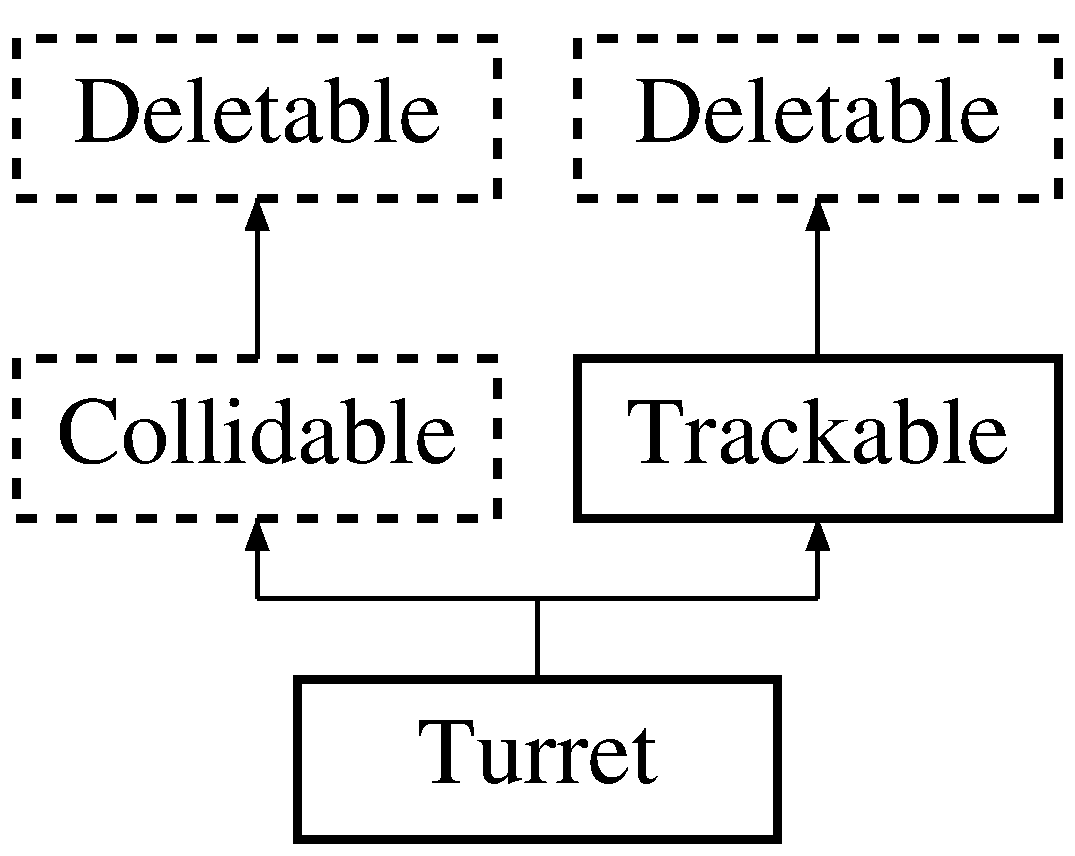
\includegraphics[height=3.000000cm]{classTurret}
\end{center}
\end{figure}
\subsection*{Public Member Functions}
\begin{DoxyCompactItemize}
\item 
\hyperlink{classTurret_ad4865ea38c314056d61968609773ec46}{Turret} (float position\-X, float position\-Y, float rotation)
\begin{DoxyCompactList}\small\item\em Constructor. \end{DoxyCompactList}\item 
virtual const \hyperlink{Structures_8h_a6d8f83e710b27d4f86c45f0bb77066e3}{entity\-\_\-type} \& \hyperlink{classTurret_a4998bf256706dc75926e683f08862b80}{get\-Type} () const 
\begin{DoxyCompactList}\small\item\em Provide type. \end{DoxyCompactList}\item 
virtual const bool \hyperlink{classTurret_a204a0c45ddcc9139cda14dcd1493fd86}{is\-Deleted} ()
\begin{DoxyCompactList}\small\item\em Determine the life state of the Turrent. \end{DoxyCompactList}\item 
virtual const float \hyperlink{classTurret_aecf0bc7d827c8f05f48b730daf00d9e4}{get\-Draw\-Position\-X} ()
\begin{DoxyCompactList}\small\item\em Retrieve the entity's x Position. \end{DoxyCompactList}\item 
virtual const float \hyperlink{classTurret_ab86c156ea9ba76d33458601aa0eb454b}{get\-Draw\-Position\-Y} ()
\begin{DoxyCompactList}\small\item\em Retrieve the entity's y Position. \end{DoxyCompactList}\item 
virtual const float \hyperlink{classTurret_a52a79fd86533f6b3d94223a60df41aaa}{get\-Draw\-Rotation} ()
\begin{DoxyCompactList}\small\item\em Retrieve the entity's Position. \end{DoxyCompactList}\item 
virtual const \hyperlink{structrect__corners}{rect\-\_\-corners} \& \hyperlink{classTurret_a48007e1c8b99645e13b24e24b850fbaa}{get\-Bounding\-Box} ()
\begin{DoxyCompactList}\small\item\em Get bounding box of entity. \end{DoxyCompactList}\item 
virtual const \hyperlink{structrect__corners}{rect\-\_\-corners} \& \hyperlink{classTurret_ad17a5c236d681627bbea6bb99b2374b0}{get\-Aligned\-Bounding\-Box} ()
\begin{DoxyCompactList}\small\item\em Get Axis Aligned bounding box of entity. \end{DoxyCompactList}\item 
virtual const int \hyperlink{classTurret_a047fe39c0367cc0896c43ac6fadfd2b6}{set\-Blocked} (const \hyperlink{Structures_8h_a6fef29d9424addfa69bdd2a379424896}{blocked\-\_\-status} obstruction\-\_\-type)
\begin{DoxyCompactList}\small\item\em Set blocked state of entity. \end{DoxyCompactList}\item 
virtual void \hyperlink{classTurret_a1cafbfb89d052d03c8e7db8b0668a75d}{set\-Unblocked} ()
\begin{DoxyCompactList}\small\item\em Unset the blocked state of the entity. \end{DoxyCompactList}\item 
virtual void \hyperlink{classTurret_a2f558a151cc9c7e7f2158c71f71261cb}{set\-Collided} ()
\begin{DoxyCompactList}\small\item\em Set collision state of entity. \end{DoxyCompactList}\item 
virtual const float \hyperlink{classTurret_a3e713aaf3b26c4dfc49893b4a7796dfd}{get\-Position\-X} ()
\begin{DoxyCompactList}\small\item\em Get the current x co-\/ordinates of \hyperlink{classTrackable}{Trackable} object. \end{DoxyCompactList}\item 
virtual const float \hyperlink{classTurret_a9d331d408eec415f38ea8249fb0ad3ef}{get\-Position\-Y} ()
\begin{DoxyCompactList}\small\item\em Get the current y co-\/ordinates of \hyperlink{classTrackable}{Trackable} object. \end{DoxyCompactList}\item 
virtual const float \hyperlink{classTurret_a7a6d4d2ca7bd5c1c4869298e77e3f1f5}{get\-Orientation} ()
\begin{DoxyCompactList}\small\item\em Get the current orientation of \hyperlink{classTrackable}{Trackable} object. \end{DoxyCompactList}\item 
virtual const \hyperlink{structrect__corners}{rect\-\_\-corners} \& \hyperlink{classTurret_ac39a14672e27fd2399b57386a55b5c04}{get\-Tracking\-Bounding\-Box} ()
\begin{DoxyCompactList}\small\item\em Get the bounding box relevant for line-\/of-\/fire detection. \end{DoxyCompactList}\item 
void \hyperlink{classTurret_a7e66153beba3e6526d1c26be106d7269}{rotate\-Turret} ()
\begin{DoxyCompactList}\small\item\em Rotates the \hyperlink{classTurret}{Turret} by its set value. \end{DoxyCompactList}\item 
virtual \hyperlink{classTurret_add5c91873b2baa27a3aa7a2a4c55e58c}{$\sim$\-Turret} ()
\begin{DoxyCompactList}\small\item\em Destructor. \end{DoxyCompactList}\end{DoxyCompactItemize}
\subsection*{Private Attributes}
\begin{DoxyCompactItemize}
\item 
bool \hyperlink{classTurret_aceb63c533fdc7b332addf9de88336c9c}{\-\_\-collided\-Status}
\begin{DoxyCompactList}\small\item\em Collision state of the Turrent Entity\-: 1 for collided, 0 for not. \end{DoxyCompactList}\item 
float \hyperlink{classTurret_a5570f2cbe1ac6bd008a9fa3b79998756}{\-\_\-rotation}
\begin{DoxyCompactList}\small\item\em The angle of rotation for the Turrnet entity. \end{DoxyCompactList}\item 
\hyperlink{classOrientation}{Orientation} \hyperlink{classTurret_a71caf1801690ed81facba1f4cc99defd}{\-\_\-turret}
\begin{DoxyCompactList}\small\item\em Co-\/ordinate system for the Turrnet. \end{DoxyCompactList}\item 
\hyperlink{Structures_8h_a6d8f83e710b27d4f86c45f0bb77066e3}{entity\-\_\-type} \hyperlink{classTurret_afadbbb1f31cce1eb6b267afebebd14f0}{\-\_\-type}
\begin{DoxyCompactList}\small\item\em Enumeration type defining the turrnet. \end{DoxyCompactList}\item 
\hyperlink{classSpriteDimensions}{Sprite\-Dimensions} \hyperlink{classTurret_aca4002cdadaf5f3e9ae210ba5d2e7244}{\-\_\-sprite\-\_\-dimensions}
\begin{DoxyCompactList}\small\item\em Turrent Sprite Dimensions. \end{DoxyCompactList}\item 
const float \hyperlink{classTurret_abd03fe34cbb67d081002b4fa3b60be71}{\-\_\-rotation\-\_\-rate}
\begin{DoxyCompactList}\small\item\em Default value for rotation rate. \end{DoxyCompactList}\end{DoxyCompactItemize}


\subsection{Detailed Description}


Definition at line 23 of file Turret.\-h.



\subsection{Constructor \& Destructor Documentation}
\hypertarget{classTurret_ad4865ea38c314056d61968609773ec46}{\index{Turret@{Turret}!Turret@{Turret}}
\index{Turret@{Turret}!Turret@{Turret}}
\subsubsection[{Turret}]{\setlength{\rightskip}{0pt plus 5cm}Turret\-::\-Turret (
\begin{DoxyParamCaption}
\item[{float}]{position\-X, }
\item[{float}]{position\-Y, }
\item[{float}]{rotation}
\end{DoxyParamCaption}
)}}\label{classTurret_ad4865ea38c314056d61968609773ec46}


Constructor. 



Definition at line 13 of file Turret.\-cpp.



References \-\_\-collided\-Status, \-\_\-sprite\-\_\-dimensions, \-\_\-turret, \-\_\-type, Orientation\-::get\-Origin\-X(), Orientation\-::get\-Origin\-Y(), Orientation\-::get\-Rotation(), Orientation\-::set\-Height(), Orientation\-::set\-Width(), turret, Sprite\-Dimensions\-::turret\-\_\-sprite\-\_\-x, and Sprite\-Dimensions\-::turret\-\_\-sprite\-\_\-y.


\begin{DoxyCode}
13                                                               :
14     \hyperlink{classTurret_a5570f2cbe1ac6bd008a9fa3b79998756}{\_rotation}(rotation),
15     \hyperlink{classTurret_a71caf1801690ed81facba1f4cc99defd}{\_turret}(positionX, positionY, 0, 0,rotation,\textcolor{keyword}{false}),
16     \hyperlink{classTurret_afadbbb1f31cce1eb6b267afebebd14f0}{\_type}(\hyperlink{Structures_8h_a6d8f83e710b27d4f86c45f0bb77066e3a85c730ac9ffc13ac94e6e860579928a1}{turret}),
17     \hyperlink{classTurret_aca4002cdadaf5f3e9ae210ba5d2e7244}{\_sprite\_dimensions}(),
18     \hyperlink{classTurret_abd03fe34cbb67d081002b4fa3b60be71}{\_rotation\_rate}(-2)
19 \{
20     \textcolor{comment}{//Error input checking}
21     \textcolor{keywordflow}{if} (\hyperlink{classTurret_a71caf1801690ed81facba1f4cc99defd}{\_turret}.\hyperlink{classOrientation_a4d6b853f2ac00965d29e5bc36b94c949}{getOriginX}() < 0) \textcolor{keywordflow}{throw} 
      \hyperlink{classInvalidConstructorArgumentsTurret}{InvalidConstructorArgumentsTurret}();
22     \textcolor{keywordflow}{if} (\hyperlink{classTurret_a71caf1801690ed81facba1f4cc99defd}{\_turret}.\hyperlink{classOrientation_ae60c88b0525d6e536a1a068d3a99f74c}{getOriginY}() < 0) \textcolor{keywordflow}{throw} 
      \hyperlink{classInvalidConstructorArgumentsTurret}{InvalidConstructorArgumentsTurret}();
23     \textcolor{keywordflow}{if} (\hyperlink{classTurret_a71caf1801690ed81facba1f4cc99defd}{\_turret}.\hyperlink{classOrientation_ab3568e037a7dc7799d557f2bc6a3cf7d}{getRotation}() < 0) \textcolor{keywordflow}{throw} 
      \hyperlink{classInvalidConstructorArgumentsTurret}{InvalidConstructorArgumentsTurret}();
24     \textcolor{keywordflow}{if} (\hyperlink{classTurret_afadbbb1f31cce1eb6b267afebebd14f0}{\_type} != \hyperlink{Structures_8h_a6d8f83e710b27d4f86c45f0bb77066e3a85c730ac9ffc13ac94e6e860579928a1}{turret}) \textcolor{keywordflow}{throw} \hyperlink{classInvalidConstructorArgumentsTurret}{InvalidConstructorArgumentsTurret}
      ();
25 
26     \hyperlink{classTurret_a71caf1801690ed81facba1f4cc99defd}{\_turret}.\hyperlink{classOrientation_a1b5cd490e5bbbe2b8d683be389dbcbbe}{setWidth}(\hyperlink{classTurret_aca4002cdadaf5f3e9ae210ba5d2e7244}{\_sprite\_dimensions}.
      \hyperlink{classSpriteDimensions_ad876e1e5dea420fe80462709c8ec2d5c}{turret\_sprite\_x});
27     \hyperlink{classTurret_a71caf1801690ed81facba1f4cc99defd}{\_turret}.\hyperlink{classOrientation_a1adca89bc32128e2ca1cb937357f5006}{setHeight}(\hyperlink{classTurret_aca4002cdadaf5f3e9ae210ba5d2e7244}{\_sprite\_dimensions}.
      \hyperlink{classSpriteDimensions_a1b808c73bd915776ec6b8c10120adeae}{turret\_sprite\_y});
28     \hyperlink{classTurret_aceb63c533fdc7b332addf9de88336c9c}{\_collidedStatus} = 0;
29 \}
\end{DoxyCode}
\hypertarget{classTurret_add5c91873b2baa27a3aa7a2a4c55e58c}{\index{Turret@{Turret}!$\sim$\-Turret@{$\sim$\-Turret}}
\index{$\sim$\-Turret@{$\sim$\-Turret}!Turret@{Turret}}
\subsubsection[{$\sim$\-Turret}]{\setlength{\rightskip}{0pt plus 5cm}Turret\-::$\sim$\-Turret (
\begin{DoxyParamCaption}
{}
\end{DoxyParamCaption}
)\hspace{0.3cm}{\ttfamily [virtual]}}}\label{classTurret_add5c91873b2baa27a3aa7a2a4c55e58c}


Destructor. 



Definition at line 106 of file Turret.\-cpp.


\begin{DoxyCode}
107 \{
108     \textcolor{comment}{// Can addd some arguments here}
109 \}
\end{DoxyCode}


\subsection{Member Function Documentation}
\hypertarget{classTurret_ad17a5c236d681627bbea6bb99b2374b0}{\index{Turret@{Turret}!get\-Aligned\-Bounding\-Box@{get\-Aligned\-Bounding\-Box}}
\index{get\-Aligned\-Bounding\-Box@{get\-Aligned\-Bounding\-Box}!Turret@{Turret}}
\subsubsection[{get\-Aligned\-Bounding\-Box}]{\setlength{\rightskip}{0pt plus 5cm}const {\bf rect\-\_\-corners} \& Turret\-::get\-Aligned\-Bounding\-Box (
\begin{DoxyParamCaption}
{}
\end{DoxyParamCaption}
)\hspace{0.3cm}{\ttfamily [virtual]}}}\label{classTurret_ad17a5c236d681627bbea6bb99b2374b0}


Get Axis Aligned bounding box of entity. 



Implements \hyperlink{classCollidable_a6909df57a0915f044d5d967a3be086f3}{Collidable}.



Definition at line 61 of file Turret.\-cpp.



References \-\_\-turret, and Orientation\-::get\-Aligned\-Global\-Bounds().


\begin{DoxyCode}
62 \{
63     \textcolor{keywordflow}{return} \hyperlink{classTurret_a71caf1801690ed81facba1f4cc99defd}{\_turret}.\hyperlink{classOrientation_a5cc606289f774c8561af98d183586199}{getAlignedGlobalBounds}();
64 \}
\end{DoxyCode}
\hypertarget{classTurret_a48007e1c8b99645e13b24e24b850fbaa}{\index{Turret@{Turret}!get\-Bounding\-Box@{get\-Bounding\-Box}}
\index{get\-Bounding\-Box@{get\-Bounding\-Box}!Turret@{Turret}}
\subsubsection[{get\-Bounding\-Box}]{\setlength{\rightskip}{0pt plus 5cm}const {\bf rect\-\_\-corners} \& Turret\-::get\-Bounding\-Box (
\begin{DoxyParamCaption}
{}
\end{DoxyParamCaption}
)\hspace{0.3cm}{\ttfamily [virtual]}}}\label{classTurret_a48007e1c8b99645e13b24e24b850fbaa}


Get bounding box of entity. 



Implements \hyperlink{classCollidable_a3436effdcd9bea230f4a1aa32b8dd8ab}{Collidable}.



Definition at line 56 of file Turret.\-cpp.



References \-\_\-turret, and Orientation\-::get\-Global\-Bounds().


\begin{DoxyCode}
57 \{
58     \textcolor{keywordflow}{return} \hyperlink{classTurret_a71caf1801690ed81facba1f4cc99defd}{\_turret}.\hyperlink{classOrientation_a950dfe84e548582d8c3c573b5ff5fe42}{getGlobalBounds}();
59 \}
\end{DoxyCode}
\hypertarget{classTurret_aecf0bc7d827c8f05f48b730daf00d9e4}{\index{Turret@{Turret}!get\-Draw\-Position\-X@{get\-Draw\-Position\-X}}
\index{get\-Draw\-Position\-X@{get\-Draw\-Position\-X}!Turret@{Turret}}
\subsubsection[{get\-Draw\-Position\-X}]{\setlength{\rightskip}{0pt plus 5cm}const float Turret\-::get\-Draw\-Position\-X (
\begin{DoxyParamCaption}
{}
\end{DoxyParamCaption}
)\hspace{0.3cm}{\ttfamily [virtual]}}}\label{classTurret_aecf0bc7d827c8f05f48b730daf00d9e4}


Retrieve the entity's x Position. 



Implements \hyperlink{classDeletable_ac14ea0c5986d50ba3ba454f89c87b8fe}{Deletable}.



Definition at line 41 of file Turret.\-cpp.



References \-\_\-turret, and Orientation\-::get\-Origin\-X().


\begin{DoxyCode}
42 \{
43     \textcolor{keywordflow}{return} \hyperlink{classTurret_a71caf1801690ed81facba1f4cc99defd}{\_turret}.\hyperlink{classOrientation_a4d6b853f2ac00965d29e5bc36b94c949}{getOriginX}();
44 \}
\end{DoxyCode}
\hypertarget{classTurret_ab86c156ea9ba76d33458601aa0eb454b}{\index{Turret@{Turret}!get\-Draw\-Position\-Y@{get\-Draw\-Position\-Y}}
\index{get\-Draw\-Position\-Y@{get\-Draw\-Position\-Y}!Turret@{Turret}}
\subsubsection[{get\-Draw\-Position\-Y}]{\setlength{\rightskip}{0pt plus 5cm}const float Turret\-::get\-Draw\-Position\-Y (
\begin{DoxyParamCaption}
{}
\end{DoxyParamCaption}
)\hspace{0.3cm}{\ttfamily [virtual]}}}\label{classTurret_ab86c156ea9ba76d33458601aa0eb454b}


Retrieve the entity's y Position. 



Implements \hyperlink{classDeletable_a2a88d7e40c56902a3d3d8f668e9d126d}{Deletable}.



Definition at line 46 of file Turret.\-cpp.



References \-\_\-turret, and Orientation\-::get\-Origin\-Y().


\begin{DoxyCode}
47 \{
48     \textcolor{keywordflow}{return} \hyperlink{classTurret_a71caf1801690ed81facba1f4cc99defd}{\_turret}.\hyperlink{classOrientation_ae60c88b0525d6e536a1a068d3a99f74c}{getOriginY}();
49 \}
\end{DoxyCode}
\hypertarget{classTurret_a52a79fd86533f6b3d94223a60df41aaa}{\index{Turret@{Turret}!get\-Draw\-Rotation@{get\-Draw\-Rotation}}
\index{get\-Draw\-Rotation@{get\-Draw\-Rotation}!Turret@{Turret}}
\subsubsection[{get\-Draw\-Rotation}]{\setlength{\rightskip}{0pt plus 5cm}const float Turret\-::get\-Draw\-Rotation (
\begin{DoxyParamCaption}
{}
\end{DoxyParamCaption}
)\hspace{0.3cm}{\ttfamily [virtual]}}}\label{classTurret_a52a79fd86533f6b3d94223a60df41aaa}


Retrieve the entity's Position. 



Implements \hyperlink{classDeletable_ad7061a6bef3efce030aa5abbc7646d47}{Deletable}.



Definition at line 51 of file Turret.\-cpp.



References \-\_\-turret, and Orientation\-::get\-Rotation().


\begin{DoxyCode}
52 \{
53     \textcolor{keywordflow}{return} \hyperlink{classTurret_a71caf1801690ed81facba1f4cc99defd}{\_turret}.\hyperlink{classOrientation_ab3568e037a7dc7799d557f2bc6a3cf7d}{getRotation}();
54 \}
\end{DoxyCode}
\hypertarget{classTurret_a7a6d4d2ca7bd5c1c4869298e77e3f1f5}{\index{Turret@{Turret}!get\-Orientation@{get\-Orientation}}
\index{get\-Orientation@{get\-Orientation}!Turret@{Turret}}
\subsubsection[{get\-Orientation}]{\setlength{\rightskip}{0pt plus 5cm}const float Turret\-::get\-Orientation (
\begin{DoxyParamCaption}
{}
\end{DoxyParamCaption}
)\hspace{0.3cm}{\ttfamily [virtual]}}}\label{classTurret_a7a6d4d2ca7bd5c1c4869298e77e3f1f5}


Get the current orientation of \hyperlink{classTrackable}{Trackable} object. 



Implements \hyperlink{classTrackable_afc6b5126b82395a5155cfe76250f92dd}{Trackable}.



Definition at line 91 of file Turret.\-cpp.



References \-\_\-turret, and Orientation\-::get\-Rotation().



Referenced by T\-E\-S\-T().


\begin{DoxyCode}
92 \{
93     \textcolor{keywordflow}{return} \hyperlink{classTurret_a71caf1801690ed81facba1f4cc99defd}{\_turret}.\hyperlink{classOrientation_ab3568e037a7dc7799d557f2bc6a3cf7d}{getRotation}();
94 \}
\end{DoxyCode}
\hypertarget{classTurret_a3e713aaf3b26c4dfc49893b4a7796dfd}{\index{Turret@{Turret}!get\-Position\-X@{get\-Position\-X}}
\index{get\-Position\-X@{get\-Position\-X}!Turret@{Turret}}
\subsubsection[{get\-Position\-X}]{\setlength{\rightskip}{0pt plus 5cm}const float Turret\-::get\-Position\-X (
\begin{DoxyParamCaption}
{}
\end{DoxyParamCaption}
)\hspace{0.3cm}{\ttfamily [virtual]}}}\label{classTurret_a3e713aaf3b26c4dfc49893b4a7796dfd}


Get the current x co-\/ordinates of \hyperlink{classTrackable}{Trackable} object. 



Implements \hyperlink{classTrackable_ab167af97aef9656403ee2d28adaf3149}{Trackable}.



Definition at line 81 of file Turret.\-cpp.



References \-\_\-turret, and Orientation\-::get\-Origin\-X().


\begin{DoxyCode}
82 \{
83     \textcolor{keywordflow}{return} \hyperlink{classTurret_a71caf1801690ed81facba1f4cc99defd}{\_turret}.\hyperlink{classOrientation_a4d6b853f2ac00965d29e5bc36b94c949}{getOriginX}();
84 \}
\end{DoxyCode}
\hypertarget{classTurret_a9d331d408eec415f38ea8249fb0ad3ef}{\index{Turret@{Turret}!get\-Position\-Y@{get\-Position\-Y}}
\index{get\-Position\-Y@{get\-Position\-Y}!Turret@{Turret}}
\subsubsection[{get\-Position\-Y}]{\setlength{\rightskip}{0pt plus 5cm}const float Turret\-::get\-Position\-Y (
\begin{DoxyParamCaption}
{}
\end{DoxyParamCaption}
)\hspace{0.3cm}{\ttfamily [virtual]}}}\label{classTurret_a9d331d408eec415f38ea8249fb0ad3ef}


Get the current y co-\/ordinates of \hyperlink{classTrackable}{Trackable} object. 



Implements \hyperlink{classTrackable_add27867f4ebf30f1fe7c3f94b4d7f4d5}{Trackable}.



Definition at line 86 of file Turret.\-cpp.



References \-\_\-turret, and Orientation\-::get\-Origin\-Y().


\begin{DoxyCode}
87 \{
88     \textcolor{keywordflow}{return} \hyperlink{classTurret_a71caf1801690ed81facba1f4cc99defd}{\_turret}.\hyperlink{classOrientation_ae60c88b0525d6e536a1a068d3a99f74c}{getOriginY}();
89 \}
\end{DoxyCode}
\hypertarget{classTurret_ac39a14672e27fd2399b57386a55b5c04}{\index{Turret@{Turret}!get\-Tracking\-Bounding\-Box@{get\-Tracking\-Bounding\-Box}}
\index{get\-Tracking\-Bounding\-Box@{get\-Tracking\-Bounding\-Box}!Turret@{Turret}}
\subsubsection[{get\-Tracking\-Bounding\-Box}]{\setlength{\rightskip}{0pt plus 5cm}const {\bf rect\-\_\-corners} \& Turret\-::get\-Tracking\-Bounding\-Box (
\begin{DoxyParamCaption}
{}
\end{DoxyParamCaption}
)\hspace{0.3cm}{\ttfamily [virtual]}}}\label{classTurret_ac39a14672e27fd2399b57386a55b5c04}


Get the bounding box relevant for line-\/of-\/fire detection. 



Implements \hyperlink{classTrackable_a79826040547e1ca65775223f26c37648}{Trackable}.



Definition at line 96 of file Turret.\-cpp.



References \-\_\-turret, and Orientation\-::get\-Global\-Bounds().


\begin{DoxyCode}
97 \{
98     \textcolor{keywordflow}{return} \hyperlink{classTurret_a71caf1801690ed81facba1f4cc99defd}{\_turret}.\hyperlink{classOrientation_a950dfe84e548582d8c3c573b5ff5fe42}{getGlobalBounds}();
99 \}
\end{DoxyCode}
\hypertarget{classTurret_a4998bf256706dc75926e683f08862b80}{\index{Turret@{Turret}!get\-Type@{get\-Type}}
\index{get\-Type@{get\-Type}!Turret@{Turret}}
\subsubsection[{get\-Type}]{\setlength{\rightskip}{0pt plus 5cm}const {\bf entity\-\_\-type} \& Turret\-::get\-Type (
\begin{DoxyParamCaption}
{}
\end{DoxyParamCaption}
) const\hspace{0.3cm}{\ttfamily [virtual]}}}\label{classTurret_a4998bf256706dc75926e683f08862b80}


Provide type. 



Implements \hyperlink{classDeletable_af8a0208abc297180873692f4215fe50f}{Deletable}.



Definition at line 31 of file Turret.\-cpp.



References \-\_\-type.


\begin{DoxyCode}
32 \{
33     \textcolor{keywordflow}{return} \hyperlink{classTurret_afadbbb1f31cce1eb6b267afebebd14f0}{\_type};
34 \}
\end{DoxyCode}
\hypertarget{classTurret_a204a0c45ddcc9139cda14dcd1493fd86}{\index{Turret@{Turret}!is\-Deleted@{is\-Deleted}}
\index{is\-Deleted@{is\-Deleted}!Turret@{Turret}}
\subsubsection[{is\-Deleted}]{\setlength{\rightskip}{0pt plus 5cm}const bool Turret\-::is\-Deleted (
\begin{DoxyParamCaption}
{}
\end{DoxyParamCaption}
)\hspace{0.3cm}{\ttfamily [virtual]}}}\label{classTurret_a204a0c45ddcc9139cda14dcd1493fd86}


Determine the life state of the Turrent. 



Implements \hyperlink{classDeletable_a6572440c291077cf52bf21288c6cd25c}{Deletable}.



Definition at line 36 of file Turret.\-cpp.



References \-\_\-collided\-Status.


\begin{DoxyCode}
37 \{
38     \textcolor{keywordflow}{return} \hyperlink{classTurret_aceb63c533fdc7b332addf9de88336c9c}{\_collidedStatus};
39 \}
\end{DoxyCode}
\hypertarget{classTurret_a7e66153beba3e6526d1c26be106d7269}{\index{Turret@{Turret}!rotate\-Turret@{rotate\-Turret}}
\index{rotate\-Turret@{rotate\-Turret}!Turret@{Turret}}
\subsubsection[{rotate\-Turret}]{\setlength{\rightskip}{0pt plus 5cm}void Turret\-::rotate\-Turret (
\begin{DoxyParamCaption}
{}
\end{DoxyParamCaption}
)}}\label{classTurret_a7e66153beba3e6526d1c26be106d7269}


Rotates the \hyperlink{classTurret}{Turret} by its set value. 



Definition at line 101 of file Turret.\-cpp.



References \-\_\-rotation\-\_\-rate, \-\_\-turret, and Orientation\-::rotate().



Referenced by T\-E\-S\-T().


\begin{DoxyCode}
102 \{
103     \hyperlink{classTurret_a71caf1801690ed81facba1f4cc99defd}{\_turret}.\hyperlink{classOrientation_aa9e115b7f4ab487e3af532592416b247}{rotate}(\hyperlink{classTurret_abd03fe34cbb67d081002b4fa3b60be71}{\_rotation\_rate});
104 \}
\end{DoxyCode}
\hypertarget{classTurret_a047fe39c0367cc0896c43ac6fadfd2b6}{\index{Turret@{Turret}!set\-Blocked@{set\-Blocked}}
\index{set\-Blocked@{set\-Blocked}!Turret@{Turret}}
\subsubsection[{set\-Blocked}]{\setlength{\rightskip}{0pt plus 5cm}const int Turret\-::set\-Blocked (
\begin{DoxyParamCaption}
\item[{const {\bf blocked\-\_\-status}}]{obstruction\-\_\-type}
\end{DoxyParamCaption}
)\hspace{0.3cm}{\ttfamily [virtual]}}}\label{classTurret_a047fe39c0367cc0896c43ac6fadfd2b6}


Set blocked state of entity. 



Implements \hyperlink{classCollidable_a6d312198ba82d26b5e360733bb87a2f0}{Collidable}.



Definition at line 66 of file Turret.\-cpp.


\begin{DoxyCode}
67 \{
68     \textcolor{keywordflow}{return} 1;
69 \}
\end{DoxyCode}
\hypertarget{classTurret_a2f558a151cc9c7e7f2158c71f71261cb}{\index{Turret@{Turret}!set\-Collided@{set\-Collided}}
\index{set\-Collided@{set\-Collided}!Turret@{Turret}}
\subsubsection[{set\-Collided}]{\setlength{\rightskip}{0pt plus 5cm}void Turret\-::set\-Collided (
\begin{DoxyParamCaption}
{}
\end{DoxyParamCaption}
)\hspace{0.3cm}{\ttfamily [virtual]}}}\label{classTurret_a2f558a151cc9c7e7f2158c71f71261cb}


Set collision state of entity. 



Implements \hyperlink{classCollidable_a5ea0417bea000712171bbe5531705082}{Collidable}.



Definition at line 76 of file Turret.\-cpp.



References \-\_\-collided\-Status.


\begin{DoxyCode}
77 \{
78     \hyperlink{classTurret_aceb63c533fdc7b332addf9de88336c9c}{\_collidedStatus} = 1;
79 \}
\end{DoxyCode}
\hypertarget{classTurret_a1cafbfb89d052d03c8e7db8b0668a75d}{\index{Turret@{Turret}!set\-Unblocked@{set\-Unblocked}}
\index{set\-Unblocked@{set\-Unblocked}!Turret@{Turret}}
\subsubsection[{set\-Unblocked}]{\setlength{\rightskip}{0pt plus 5cm}void Turret\-::set\-Unblocked (
\begin{DoxyParamCaption}
{}
\end{DoxyParamCaption}
)\hspace{0.3cm}{\ttfamily [virtual]}}}\label{classTurret_a1cafbfb89d052d03c8e7db8b0668a75d}


Unset the blocked state of the entity. 



Implements \hyperlink{classCollidable_a817d864d0640bc6bcb13bbecf14ddf31}{Collidable}.



Definition at line 71 of file Turret.\-cpp.


\begin{DoxyCode}
72 \{
73     \textcolor{comment}{//Do nothing here!}
74 \}
\end{DoxyCode}


\subsection{Member Data Documentation}
\hypertarget{classTurret_aceb63c533fdc7b332addf9de88336c9c}{\index{Turret@{Turret}!\-\_\-collided\-Status@{\-\_\-collided\-Status}}
\index{\-\_\-collided\-Status@{\-\_\-collided\-Status}!Turret@{Turret}}
\subsubsection[{\-\_\-collided\-Status}]{\setlength{\rightskip}{0pt plus 5cm}bool Turret\-::\-\_\-collided\-Status\hspace{0.3cm}{\ttfamily [private]}}}\label{classTurret_aceb63c533fdc7b332addf9de88336c9c}


Collision state of the Turrent Entity\-: 1 for collided, 0 for not. 



Definition at line 65 of file Turret.\-h.



Referenced by is\-Deleted(), set\-Collided(), and Turret().

\hypertarget{classTurret_a5570f2cbe1ac6bd008a9fa3b79998756}{\index{Turret@{Turret}!\-\_\-rotation@{\-\_\-rotation}}
\index{\-\_\-rotation@{\-\_\-rotation}!Turret@{Turret}}
\subsubsection[{\-\_\-rotation}]{\setlength{\rightskip}{0pt plus 5cm}float Turret\-::\-\_\-rotation\hspace{0.3cm}{\ttfamily [private]}}}\label{classTurret_a5570f2cbe1ac6bd008a9fa3b79998756}


The angle of rotation for the Turrnet entity. 



Definition at line 67 of file Turret.\-h.

\hypertarget{classTurret_abd03fe34cbb67d081002b4fa3b60be71}{\index{Turret@{Turret}!\-\_\-rotation\-\_\-rate@{\-\_\-rotation\-\_\-rate}}
\index{\-\_\-rotation\-\_\-rate@{\-\_\-rotation\-\_\-rate}!Turret@{Turret}}
\subsubsection[{\-\_\-rotation\-\_\-rate}]{\setlength{\rightskip}{0pt plus 5cm}const float Turret\-::\-\_\-rotation\-\_\-rate\hspace{0.3cm}{\ttfamily [private]}}}\label{classTurret_abd03fe34cbb67d081002b4fa3b60be71}


Default value for rotation rate. 



Definition at line 75 of file Turret.\-h.



Referenced by rotate\-Turret().

\hypertarget{classTurret_aca4002cdadaf5f3e9ae210ba5d2e7244}{\index{Turret@{Turret}!\-\_\-sprite\-\_\-dimensions@{\-\_\-sprite\-\_\-dimensions}}
\index{\-\_\-sprite\-\_\-dimensions@{\-\_\-sprite\-\_\-dimensions}!Turret@{Turret}}
\subsubsection[{\-\_\-sprite\-\_\-dimensions}]{\setlength{\rightskip}{0pt plus 5cm}{\bf Sprite\-Dimensions} Turret\-::\-\_\-sprite\-\_\-dimensions\hspace{0.3cm}{\ttfamily [private]}}}\label{classTurret_aca4002cdadaf5f3e9ae210ba5d2e7244}


Turrent Sprite Dimensions. 



Definition at line 73 of file Turret.\-h.



Referenced by Turret().

\hypertarget{classTurret_a71caf1801690ed81facba1f4cc99defd}{\index{Turret@{Turret}!\-\_\-turret@{\-\_\-turret}}
\index{\-\_\-turret@{\-\_\-turret}!Turret@{Turret}}
\subsubsection[{\-\_\-turret}]{\setlength{\rightskip}{0pt plus 5cm}{\bf Orientation} Turret\-::\-\_\-turret\hspace{0.3cm}{\ttfamily [private]}}}\label{classTurret_a71caf1801690ed81facba1f4cc99defd}


Co-\/ordinate system for the Turrnet. 



Definition at line 69 of file Turret.\-h.



Referenced by get\-Aligned\-Bounding\-Box(), get\-Bounding\-Box(), get\-Draw\-Position\-X(), get\-Draw\-Position\-Y(), get\-Draw\-Rotation(), get\-Orientation(), get\-Position\-X(), get\-Position\-Y(), get\-Tracking\-Bounding\-Box(), rotate\-Turret(), and Turret().

\hypertarget{classTurret_afadbbb1f31cce1eb6b267afebebd14f0}{\index{Turret@{Turret}!\-\_\-type@{\-\_\-type}}
\index{\-\_\-type@{\-\_\-type}!Turret@{Turret}}
\subsubsection[{\-\_\-type}]{\setlength{\rightskip}{0pt plus 5cm}{\bf entity\-\_\-type} Turret\-::\-\_\-type\hspace{0.3cm}{\ttfamily [private]}}}\label{classTurret_afadbbb1f31cce1eb6b267afebebd14f0}


Enumeration type defining the turrnet. 



Definition at line 71 of file Turret.\-h.



Referenced by get\-Type(), and Turret().



The documentation for this class was generated from the following files\-:\begin{DoxyCompactItemize}
\item 
\hyperlink{Turret_8h}{Turret.\-h}\item 
\hyperlink{Turret_8cpp}{Turret.\-cpp}\end{DoxyCompactItemize}

\hypertarget{classTurretManager}{\section{Turret\-Manager Class Reference}
\label{classTurretManager}\index{Turret\-Manager@{Turret\-Manager}}
}


\hyperlink{classManager}{Manager} responsible for controlling the turrets rotation.  




{\ttfamily \#include $<$Turret\-Manager.\-h$>$}

Inheritance diagram for Turret\-Manager\-:\begin{figure}[H]
\begin{center}
\leavevmode
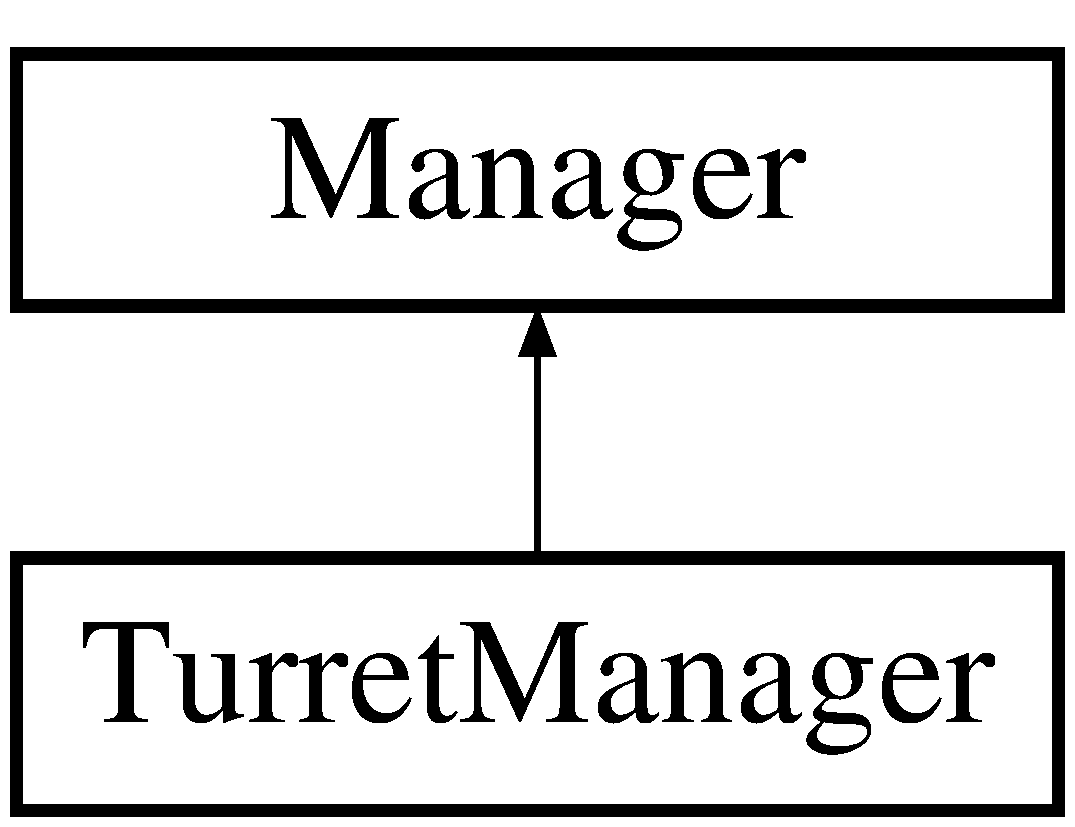
\includegraphics[height=2.000000cm]{classTurretManager}
\end{center}
\end{figure}
\subsection*{Public Member Functions}
\begin{DoxyCompactItemize}
\item 
\hyperlink{classTurretManager_a81d31a8afa69beed2e1e9ee92a148b62}{Turret\-Manager} ()
\item 
void \hyperlink{classTurretManager_a3339500bc4e12ed437681876ca702bd3}{manage} ()
\begin{DoxyCompactList}\small\item\em Manage turret movements. \end{DoxyCompactList}\item 
void \hyperlink{classTurretManager_a61a5c5fe1961ca9483271da3aeac0489}{add\-New\-Entity} (std\-::weak\-\_\-ptr$<$ \hyperlink{classTurret}{Turret} $>$ new\-\_\-entity)
\begin{DoxyCompactList}\small\item\em Add a new weak pointer to a game turrt. \end{DoxyCompactList}\item 
virtual \hyperlink{classTurretManager_a223f756a6c40df2487a0b98b640c3155}{$\sim$\-Turret\-Manager} ()
\end{DoxyCompactItemize}
\subsection*{Private Member Functions}
\begin{DoxyCompactItemize}
\item 
void \hyperlink{classTurretManager_af403fc2ffe83d4c3b017251dbcbd52f6}{remove\-Garbage} ()
\begin{DoxyCompactList}\small\item\em Removed weak pointers of objects that have been deleted. \end{DoxyCompactList}\end{DoxyCompactItemize}
\subsection*{Private Attributes}
\begin{DoxyCompactItemize}
\item 
std\-::vector$<$ std\-::weak\-\_\-ptr\\*
$<$ \hyperlink{classTurret}{Turret} $>$ $>$ \hyperlink{classTurretManager_a1089603cbf805dfb737b2a47d462a9bb}{\-\_\-turretables}
\begin{DoxyCompactList}\small\item\em Container for all weak pointers to game turret entities. \end{DoxyCompactList}\end{DoxyCompactItemize}


\subsection{Detailed Description}
\hyperlink{classManager}{Manager} responsible for controlling the turrets rotation. 

Definition at line 17 of file Turret\-Manager.\-h.



\subsection{Constructor \& Destructor Documentation}
\hypertarget{classTurretManager_a81d31a8afa69beed2e1e9ee92a148b62}{\index{Turret\-Manager@{Turret\-Manager}!Turret\-Manager@{Turret\-Manager}}
\index{Turret\-Manager@{Turret\-Manager}!TurretManager@{Turret\-Manager}}
\subsubsection[{Turret\-Manager}]{\setlength{\rightskip}{0pt plus 5cm}Turret\-Manager\-::\-Turret\-Manager (
\begin{DoxyParamCaption}
{}
\end{DoxyParamCaption}
)}}\label{classTurretManager_a81d31a8afa69beed2e1e9ee92a148b62}


Definition at line 11 of file Turret\-Manager.\-cpp.


\begin{DoxyCode}
12 \{
13 
14 \}
\end{DoxyCode}
\hypertarget{classTurretManager_a223f756a6c40df2487a0b98b640c3155}{\index{Turret\-Manager@{Turret\-Manager}!$\sim$\-Turret\-Manager@{$\sim$\-Turret\-Manager}}
\index{$\sim$\-Turret\-Manager@{$\sim$\-Turret\-Manager}!TurretManager@{Turret\-Manager}}
\subsubsection[{$\sim$\-Turret\-Manager}]{\setlength{\rightskip}{0pt plus 5cm}Turret\-Manager\-::$\sim$\-Turret\-Manager (
\begin{DoxyParamCaption}
{}
\end{DoxyParamCaption}
)\hspace{0.3cm}{\ttfamily [virtual]}}}\label{classTurretManager_a223f756a6c40df2487a0b98b640c3155}


Definition at line 16 of file Turret\-Manager.\-cpp.


\begin{DoxyCode}
17 \{
18 
19 \}
\end{DoxyCode}


\subsection{Member Function Documentation}
\hypertarget{classTurretManager_a61a5c5fe1961ca9483271da3aeac0489}{\index{Turret\-Manager@{Turret\-Manager}!add\-New\-Entity@{add\-New\-Entity}}
\index{add\-New\-Entity@{add\-New\-Entity}!TurretManager@{Turret\-Manager}}
\subsubsection[{add\-New\-Entity}]{\setlength{\rightskip}{0pt plus 5cm}void Turret\-Manager\-::add\-New\-Entity (
\begin{DoxyParamCaption}
\item[{std\-::weak\-\_\-ptr$<$ {\bf Turret} $>$}]{new\-\_\-entity}
\end{DoxyParamCaption}
)}}\label{classTurretManager_a61a5c5fe1961ca9483271da3aeac0489}


Add a new weak pointer to a game turrt. 

All the turrets have weak pointers stored in the \hyperlink{classTurretManager}{Turret\-Manager} private vector. 

Definition at line 45 of file Turret\-Manager.\-cpp.



References \-\_\-turretables.



Referenced by Game\-::add\-Turretable(), and T\-E\-S\-T().


\begin{DoxyCode}
46 \{
47     \hyperlink{classTurretManager_a1089603cbf805dfb737b2a47d462a9bb}{\_turretables}.push\_back(new\_entity);
48 \}
\end{DoxyCode}
\hypertarget{classTurretManager_a3339500bc4e12ed437681876ca702bd3}{\index{Turret\-Manager@{Turret\-Manager}!manage@{manage}}
\index{manage@{manage}!TurretManager@{Turret\-Manager}}
\subsubsection[{manage}]{\setlength{\rightskip}{0pt plus 5cm}void Turret\-Manager\-::manage (
\begin{DoxyParamCaption}
{}
\end{DoxyParamCaption}
)}}\label{classTurretManager_a3339500bc4e12ed437681876ca702bd3}


Manage turret movements. 

All turrets are simply rotated each time the manager runs 

Definition at line 24 of file Turret\-Manager.\-cpp.



References \-\_\-turretables, and remove\-Garbage().



Referenced by Game\-::run\-All\-Managers(), and T\-E\-S\-T().


\begin{DoxyCode}
25 \{
26     \textcolor{comment}{//Clear the vector of deleted turret entities}
27     \hyperlink{classTurretManager_af403fc2ffe83d4c3b017251dbcbd52f6}{removeGarbage}();
28 
29     \textcolor{keyword}{auto} turret\_iterator = \hyperlink{classTurretManager_a1089603cbf805dfb737b2a47d462a9bb}{\_turretables}.begin();
30     \textcolor{keywordflow}{for} (; turret\_iterator !=  \hyperlink{classTurretManager_a1089603cbf805dfb737b2a47d462a9bb}{\_turretables}.end(); turret\_iterator ++)
31     \{
32         \textcolor{comment}{//Convert iterator to Weak pointer}
33         std::weak\_ptr<Turret> entity\_tur\_wp = (*turret\_iterator);
34 
35         \textcolor{comment}{//Lock as Shared Pointer}
36         std::shared\_ptr<Turret> entity\_tur\_sp = entity\_tur\_wp.lock();
37 
38         entity\_tur\_sp->rotateTurret();
39     \}
40 \}
\end{DoxyCode}
\hypertarget{classTurretManager_af403fc2ffe83d4c3b017251dbcbd52f6}{\index{Turret\-Manager@{Turret\-Manager}!remove\-Garbage@{remove\-Garbage}}
\index{remove\-Garbage@{remove\-Garbage}!TurretManager@{Turret\-Manager}}
\subsubsection[{remove\-Garbage}]{\setlength{\rightskip}{0pt plus 5cm}void Turret\-Manager\-::remove\-Garbage (
\begin{DoxyParamCaption}
{}
\end{DoxyParamCaption}
)\hspace{0.3cm}{\ttfamily [private]}}}\label{classTurretManager_af403fc2ffe83d4c3b017251dbcbd52f6}


Removed weak pointers of objects that have been deleted. 



Definition at line 53 of file Turret\-Manager.\-cpp.



References \-\_\-turretables.



Referenced by manage().


\begin{DoxyCode}
54 \{
55     \textcolor{keyword}{auto} removable = \hyperlink{classTurretManager_a1089603cbf805dfb737b2a47d462a9bb}{\_turretables}.begin();
56     \textcolor{keywordflow}{for} (; removable != \hyperlink{classTurretManager_a1089603cbf805dfb737b2a47d462a9bb}{\_turretables}.end();)
57     \{
58         \textcolor{comment}{//Convert iterator to Weak pointer}
59         std::weak\_ptr<Turret> removable\_wp = (*removable);
60         \textcolor{comment}{//Lock as Shared Pointer}
61         std::shared\_ptr<Turret> removable\_sp = removable\_wp.lock();
62         \textcolor{comment}{//Test to see if the shared pointer exists}
63         \textcolor{keywordflow}{if} (removable\_sp)
64         \{
65             removable++;
66         \}
67         \textcolor{keywordflow}{else}
68         \{
69             \hyperlink{classTurretManager_a1089603cbf805dfb737b2a47d462a9bb}{\_turretables}.erase(removable);
70         \}
71     \}
72 \}
\end{DoxyCode}


\subsection{Member Data Documentation}
\hypertarget{classTurretManager_a1089603cbf805dfb737b2a47d462a9bb}{\index{Turret\-Manager@{Turret\-Manager}!\-\_\-turretables@{\-\_\-turretables}}
\index{\-\_\-turretables@{\-\_\-turretables}!TurretManager@{Turret\-Manager}}
\subsubsection[{\-\_\-turretables}]{\setlength{\rightskip}{0pt plus 5cm}std\-::vector$<$std\-::weak\-\_\-ptr$<${\bf Turret}$>$ $>$ Turret\-Manager\-::\-\_\-turretables\hspace{0.3cm}{\ttfamily [private]}}}\label{classTurretManager_a1089603cbf805dfb737b2a47d462a9bb}


Container for all weak pointers to game turret entities. 



Definition at line 27 of file Turret\-Manager.\-h.



Referenced by add\-New\-Entity(), manage(), and remove\-Garbage().



The documentation for this class was generated from the following files\-:\begin{DoxyCompactItemize}
\item 
\hyperlink{TurretManager_8h}{Turret\-Manager.\-h}\item 
\hyperlink{TurretManager_8cpp}{Turret\-Manager.\-cpp}\end{DoxyCompactItemize}

\chapter{File Documentation}
\hypertarget{ActionData_8h}{\section{Action\-Data.\-h File Reference}
\label{ActionData_8h}\index{Action\-Data.\-h@{Action\-Data.\-h}}
}


An Abstract-\/based class providing an interface for action data containing classes.  


{\ttfamily \#include \char`\"{}Structures.\-h\char`\"{}}\\*
\subsection*{Classes}
\begin{DoxyCompactItemize}
\item 
class \hyperlink{classActionData}{Action\-Data}
\end{DoxyCompactItemize}


\subsection{Detailed Description}
An Abstract-\/based class providing an interface for action data containing classes. This class is used as a interface-\/parent for a classes which will hold action data for the game. It defines an array of pure virtual getters and setters which can be implemented in various ways for versitiliy.

\begin{DoxyAuthor}{Author}
Daniel Holmes \& Jonathan Gerrand 
\end{DoxyAuthor}
\begin{DoxyVersion}{Version}
2.\-0 
\end{DoxyVersion}
\begin{DoxyDate}{Date}
29 September 2014 
\end{DoxyDate}


Definition in file \hyperlink{ActionData_8h_source}{Action\-Data.\-h}.


\hypertarget{Barrier_8cpp}{\section{Barrier.\-cpp File Reference}
\label{Barrier_8cpp}\index{Barrier.\-cpp@{Barrier.\-cpp}}
}


Implementation for the \hyperlink{classBarrier}{Barrier} Class.  


{\ttfamily \#include \char`\"{}Barrier.\-h\char`\"{}}\\*


\subsection{Detailed Description}
Implementation for the \hyperlink{classBarrier}{Barrier} Class. This class provides a base object which can be placed around and boardering the game map. It is currectly indestructible and blocks all objects which interact with it.

\begin{DoxyAuthor}{Author}
Daniel Holmes \& Jonathan Gerrand 
\end{DoxyAuthor}
\begin{DoxyVersion}{Version}
2.\-0 
\end{DoxyVersion}
\begin{DoxyDate}{Date}
2 September 2014 
\end{DoxyDate}


Definition in file \hyperlink{Barrier_8cpp_source}{Barrier.\-cpp}.


\hypertarget{Barrier_8h}{\section{Barrier.\-h File Reference}
\label{Barrier_8h}\index{Barrier.\-h@{Barrier.\-h}}
}


A Composition-\/based class representing a simple barrier object within the game world.  


{\ttfamily \#include \char`\"{}Collidable.\-h\char`\"{}}\\*
{\ttfamily \#include \char`\"{}Structures.\-h\char`\"{}}\\*
{\ttfamily \#include \char`\"{}Orientation.\-h\char`\"{}}\\*
{\ttfamily \#include \char`\"{}Sprite\-Dimensions.\-h\char`\"{}}\\*
\subsection*{Classes}
\begin{DoxyCompactItemize}
\item 
class \hyperlink{classInvalidConstructorArgumentsBarrier}{Invalid\-Constructor\-Arguments\-Barrier}
\item 
class \hyperlink{classBarrier}{Barrier}
\end{DoxyCompactItemize}


\subsection{Detailed Description}
A Composition-\/based class representing a simple barrier object within the game world. This class provides a base object which can be placed around and boardering the game map. It is currectly indestructible and blocks all objects which interact with it.

\begin{DoxyAuthor}{Author}
Daniel Holmes \& Jonathan Gerrand 
\end{DoxyAuthor}
\begin{DoxyVersion}{Version}
2.\-0 
\end{DoxyVersion}
\begin{DoxyDate}{Date}
2 September 2014 
\end{DoxyDate}


Definition in file \hyperlink{Barrier_8h_source}{Barrier.\-h}.


\hypertarget{ClassTests_8cpp}{\section{Class\-Tests.\-cpp File Reference}
\label{ClassTests_8cpp}\index{Class\-Tests.\-cpp@{Class\-Tests.\-cpp}}
}


Unit tests for all classes. Included in single file for regression testing purposes.  


{\ttfamily \#include $<$gtest/gtest.\-h$>$}\\*
{\ttfamily \#include \char`\"{}Structures.\-h\char`\"{}}\\*
{\ttfamily \#include \char`\"{}Orientation.\-h\char`\"{}}\\*
{\ttfamily \#include \char`\"{}Game\-Management\-Data.\-h\char`\"{}}\\*
{\ttfamily \#include \char`\"{}Game\-State\-Data.\-h\char`\"{}}\\*
{\ttfamily \#include \char`\"{}Manager.\-h\char`\"{}}\\*
{\ttfamily \#include \char`\"{}Game\-State\-Manager.\-h\char`\"{}}\\*
{\ttfamily \#include \char`\"{}Collision\-Manager.\-h\char`\"{}}\\*
{\ttfamily \#include \char`\"{}Tracking\-Manager.\-h\char`\"{}}\\*
{\ttfamily \#include \char`\"{}Move\-Manager.\-h\char`\"{}}\\*
{\ttfamily \#include \char`\"{}Destruction\-Manager.\-h\char`\"{}}\\*
{\ttfamily \#include \char`\"{}Turret\-Manager.\-h\char`\"{}}\\*
{\ttfamily \#include \char`\"{}Tank.\-h\char`\"{}}\\*
{\ttfamily \#include \char`\"{}Missile.\-h\char`\"{}}\\*
{\ttfamily \#include \char`\"{}Barrier.\-h\char`\"{}}\\*
{\ttfamily \#include \char`\"{}Mine.\-h\char`\"{}}\\*
{\ttfamily \#include \char`\"{}Geometry\-Engine.\-h\char`\"{}}\\*
{\ttfamily \#include \char`\"{}Turret.\-h\char`\"{}}\\*
\subsection*{Macros}
\begin{DoxyCompactItemize}
\item 
\#define \hyperlink{ClassTests_8cpp_ad732a73881fc4402a1309791ae339341}{M\-I\-S\-S\-I\-L\-E\-\_\-\-S\-P\-E\-E\-D}~8
\item 
\#define \hyperlink{ClassTests_8cpp_a961a4321e987cb2c212acbd369495e50}{T\-A\-N\-K\-\_\-\-S\-P\-E\-E\-D}~3
\item 
\#define \hyperlink{ClassTests_8cpp_af6ef53464ca46623e9ed766edfb8f15a}{M\-I\-S\-S\-I\-L\-E\-\_\-\-R\-O\-T\-\_\-\-S\-P\-E\-E\-D}~45
\item 
\#define \hyperlink{ClassTests_8cpp_a43bc2a5f92619c101421beba01fa4fa9}{T\-A\-N\-K\-\_\-\-R\-O\-T\-\_\-\-S\-P\-E\-E\-D}~5
\item 
\#define \hyperlink{ClassTests_8cpp_a4820fe4db788d960a0beecb7da318d21}{T\-U\-R\-R\-E\-T\-\_\-\-R\-O\-T\-A\-T\-I\-O\-N\-\_\-\-S\-P\-E\-E\-D}~-\/2
\item 
\#define \hyperlink{ClassTests_8cpp_a598a3330b3c21701223ee0ca14316eca}{P\-I}~3.\-141592653589793238462643383279502884\-L
\end{DoxyCompactItemize}
\subsection*{Functions}
\begin{DoxyCompactItemize}
\item 
\hyperlink{ClassTests_8cpp_a517edf5aabb866b6e13c8ad096787443}{T\-E\-S\-T} (\hyperlink{classOrientation}{Orientation}, constructor\-Correctly\-Assigns\-Initial\-Parameters)
\begin{DoxyCompactList}\small\item\em $\ast$==============Tests for \hyperlink{classOrientation}{Orientation} Class=======$\ast$/ \end{DoxyCompactList}\item 
\hyperlink{ClassTests_8cpp_a07a04791cb3528cb0eb71189b412155b}{T\-E\-S\-T} (\hyperlink{classOrientation}{Orientation}, equality\-Opperator\-Corresctly\-Returns\-Values)
\item 
\hyperlink{ClassTests_8cpp_aef28c04d8a90cce03acd35c535e63f62}{T\-E\-S\-T} (\hyperlink{classOrientation}{Orientation}, move\-Function\-Correctly\-Changes\-Coodinates)
\item 
\hyperlink{ClassTests_8cpp_a49babdca36dd4fa09efc803464e7e648}{T\-E\-S\-T} (\hyperlink{classOrientation}{Orientation}, rotate\-Function\-Correctly\-Changes\-Coordinates)
\item 
\hyperlink{ClassTests_8cpp_a4380786b705ceefab055f69d13125d78}{T\-E\-S\-T} (\hyperlink{classOrientation}{Orientation}, get\-Global\-Bounds\-Correctly\-Returns\-Bounding\-Box)
\item 
\hyperlink{ClassTests_8cpp_a5d44e42b863157ba039b3c696bcb3fad}{T\-E\-S\-T} (\hyperlink{classOrientation}{Orientation}, throws\-Exception\-For\-Invalid\-State\-Of\-Coordinate\-Data)
\item 
\hyperlink{ClassTests_8cpp_a9970ac1db847f1ea3a7077487985c159}{T\-E\-S\-T} (\hyperlink{classTank}{Tank}, if\-Invalid\-Co\-Ordinates\-Throws\-Exception)
\begin{DoxyCompactList}\small\item\em $\ast$================================================$\ast$/ \end{DoxyCompactList}\item 
\hyperlink{ClassTests_8cpp_a6560aa3bf6047c9e6b2f8183f0ed08f4}{T\-E\-S\-T} (\hyperlink{classTank}{Tank}, returns\-Correct\-Entity\-Type)
\item 
\hyperlink{ClassTests_8cpp_af87dae29d11efba41911faef336431de}{T\-E\-S\-T} (\hyperlink{classTank}{Tank}, returns\-Correct\-Coordinates\-From\-Get\-Position)
\item 
\hyperlink{ClassTests_8cpp_a32d4fee0e739bca8298a201df874b435}{T\-E\-S\-T} (\hyperlink{classTank}{Tank}, returns\-Correct\-Coordinates\-From\-Get\-Draw\-Position)
\item 
\hyperlink{ClassTests_8cpp_a86d9942b069d800b10a3809c69965186}{T\-E\-S\-T} (\hyperlink{classTank}{Tank}, returns\-Correct\-Orientation\-Value)
\item 
\hyperlink{ClassTests_8cpp_ad63d988b859ac6dea06eae475923dbbc}{T\-E\-S\-T} (\hyperlink{classTank}{Tank}, returns\-Correct\-Draw\-Rotation\-Value)
\item 
\hyperlink{ClassTests_8cpp_a67b56db6ebcf477878f6f1fea57a5582}{T\-E\-S\-T} (\hyperlink{classTank}{Tank}, moves\-Forward\-Correctly)
\item 
\hyperlink{ClassTests_8cpp_a90b2588cda2919428cfb37b24dc47d8d}{T\-E\-S\-T} (\hyperlink{classTank}{Tank}, moves\-Backward\-Correctly)
\item 
\hyperlink{ClassTests_8cpp_a492fef8eebd3e4fd97f5780ae8dea855}{T\-E\-S\-T} (\hyperlink{classTank}{Tank}, rotates\-Left\-And\-Right\-Correctly)
\item 
\hyperlink{ClassTests_8cpp_a3e1afae7042f6569bdfc1631f71dec8d}{T\-E\-S\-T} (\hyperlink{classTank}{Tank}, boolean\-Variables\-Are\-Correctly\-Set\-And\-Retrieved)
\item 
\hyperlink{ClassTests_8cpp_ac03698654107b47243edea9a0e8740ac}{T\-E\-S\-T} (\hyperlink{classMissile}{Missile}, if\-Invalid\-Co\-Ordinates\-Throws\-Exception)
\begin{DoxyCompactList}\small\item\em $\ast$===================================================$\ast$/ \end{DoxyCompactList}\item 
\hyperlink{ClassTests_8cpp_a0c472bd3738c9685a85214942a043519}{T\-E\-S\-T} (\hyperlink{classMissile}{Missile}, returns\-Correct\-Entity\-Type)
\item 
\hyperlink{ClassTests_8cpp_aea5aaa2b7a1d8cf0e0d35806aa3fe5e0}{T\-E\-S\-T} (\hyperlink{classMissile}{Missile}, returns\-Correct\-Coordinates\-From\-Get\-Draw\-Position)
\item 
\hyperlink{ClassTests_8cpp_acb27402b1bf4dea774190c3418fe5bdc}{T\-E\-S\-T} (\hyperlink{classMissile}{Missile}, returns\-Correct\-Draw\-Rotation\-Value)
\item 
\hyperlink{ClassTests_8cpp_a05d6711d055061305eda38662bd18165}{T\-E\-S\-T} (\hyperlink{classMissile}{Missile}, moves\-Forward\-Correctly)
\item 
\hyperlink{ClassTests_8cpp_ab09807de6727cccdd3f44d0b33bc9b23}{T\-E\-S\-T} (\hyperlink{classMissile}{Missile}, moves\-Backwards\-Correctly)
\item 
\hyperlink{ClassTests_8cpp_a1e820129e32cd981015fcf8548aa58ea}{T\-E\-S\-T} (\hyperlink{classMissile}{Missile}, rotates\-Left\-And\-Right\-Correctly)
\item 
\hyperlink{ClassTests_8cpp_a6a810bf9479afc04b25978aafeb8bea6}{T\-E\-S\-T} (\hyperlink{classMissile}{Missile}, boolean\-Variables\-Are\-Correctly\-Set\-And\-Retrieved)
\item 
\hyperlink{ClassTests_8cpp_a809275f5348d4a5c5fe26f274317eab1}{T\-E\-S\-T} (\hyperlink{classBarrier}{Barrier}, if\-Invalid\-Co\-Ordinates\-Throws\-Exception)
\begin{DoxyCompactList}\small\item\em $\ast$================Tests for \hyperlink{classBarrier}{Barrier} Class============$\ast$/ \end{DoxyCompactList}\item 
\hyperlink{ClassTests_8cpp_a6945223631a8021163532d627b48f99f}{T\-E\-S\-T} (\hyperlink{classBarrier}{Barrier}, returns\-Correct\-Entity\-Type)
\item 
\hyperlink{ClassTests_8cpp_a50436486c169c85aac6de7705bbc154c}{T\-E\-S\-T} (\hyperlink{classBarrier}{Barrier}, return\-Correct\-Rectangle\-Vertices)
\item 
\hyperlink{ClassTests_8cpp_aee9a07cf1054e89f6b60960d635f3c67}{T\-E\-S\-T} (\hyperlink{classBarrier}{Barrier}, returns\-Correct\-Coordinates\-From\-Get\-Draw\-Position)
\item 
\hyperlink{ClassTests_8cpp_af5094a9f358b02ba7c468888461ca391}{T\-E\-S\-T} (\hyperlink{classBarrier}{Barrier}, returns\-Correct\-Draw\-Rotation\-Value)
\item 
\hyperlink{ClassTests_8cpp_a7cb873ed327e29d3b802d3e1cb2b896c}{T\-E\-S\-T} (\hyperlink{classMine}{Mine}, throws\-Exception\-If\-Invalid\-Coordinates\-Given)
\begin{DoxyCompactList}\small\item\em $\ast$===================================================$\ast$/ \end{DoxyCompactList}\item 
\hyperlink{ClassTests_8cpp_ad693496d7d8d18b9db4f70373196c3da}{T\-E\-S\-T} (\hyperlink{classMine}{Mine}, returns\-Correct\-Entity\-Type)
\item 
\hyperlink{ClassTests_8cpp_a09836ffa498ab6317ec0dc8975dabe7c}{T\-E\-S\-T} (\hyperlink{classMine}{Mine}, boolean\-Variables\-Are\-Correctly\-Set\-And\-Retrieved)
\item 
\hyperlink{ClassTests_8cpp_a6f134e12baacba24123f65aac1b7e5ad}{T\-E\-S\-T} (\hyperlink{classTurret}{Turret}, throws\-Exception\-If\-Invalid\-Coordinates\-Given)
\begin{DoxyCompactList}\small\item\em $\ast$===================================================$\ast$/ \end{DoxyCompactList}\item 
\hyperlink{ClassTests_8cpp_a6691b18798ade522a2a33d787d8cb9b7}{T\-E\-S\-T} (\hyperlink{classTurret}{Turret}, correctly\-Rotates\-Through\-Command)
\item 
\hyperlink{ClassTests_8cpp_a2d2434fb094bdd386c840d7470544660}{T\-E\-S\-T} (\hyperlink{classGeometryEngine}{Geometry\-Engine}, returns\-True\-If\-Rectangles\-Collided)
\begin{DoxyCompactList}\small\item\em $\ast$===================================================$\ast$/ \end{DoxyCompactList}\item 
\hyperlink{ClassTests_8cpp_ad49cce6f3cbf3a8584f9252327b81706}{T\-E\-S\-T} (\hyperlink{classGeometryEngine}{Geometry\-Engine}, returns\-False\-If\-Rectangles\-Are\-Not\-Collided)
\item 
\hyperlink{ClassTests_8cpp_aec816c8a28e245f6f802ac2e6d14fda5}{T\-E\-S\-T} (\hyperlink{classGeometryEngine}{Geometry\-Engine}, returns\-True\-If\-Overlap\-On\-All\-Axes)
\item 
\hyperlink{ClassTests_8cpp_a1ee20ffefeeb2e445344ef66afc9568c}{T\-E\-S\-T} (\hyperlink{classGeometryEngine}{Geometry\-Engine}, returns\-False\-If\-No\-Overlap\-On\-Axis\-One)
\item 
\hyperlink{ClassTests_8cpp_adc1a892283fc818b9faeabc974e92954}{T\-E\-S\-T} (\hyperlink{classGeometryEngine}{Geometry\-Engine}, returns\-False\-If\-No\-Overlap\-On\-Axis\-Two)
\item 
\hyperlink{ClassTests_8cpp_a4ea3d2cb46c9e897d2a1c7dc05215080}{T\-E\-S\-T} (\hyperlink{classGeometryEngine}{Geometry\-Engine}, returns\-False\-If\-No\-Overlap\-On\-Axis\-Three)
\item 
\hyperlink{ClassTests_8cpp_a51f981557be8189c5a747c6841f01067}{T\-E\-S\-T} (\hyperlink{classGeometryEngine}{Geometry\-Engine}, returns\-False\-If\-No\-Overlap\-On\-Axis\-Four)
\item 
\hyperlink{ClassTests_8cpp_a0297616b9fba5e745e79d5404f32afe2}{T\-E\-S\-T} (\hyperlink{classGeometryEngine}{Geometry\-Engine}, returns\-False\-If\-Tank\-Not\-In\-Line\-Of\-Fire\-Of\-Turret)
\item 
\hyperlink{ClassTests_8cpp_ac0fdc3992c8395f47871c4949be6c8e3}{T\-E\-S\-T} (\hyperlink{classGeometryEngine}{Geometry\-Engine}, correctly\-Identifies\-Relative\-Positions\-Of\-Bounding\-Boxes\-\_\-\-Above)
\item 
\hyperlink{ClassTests_8cpp_a7b632666a8d8dc9ff223215b7ebb9e68}{T\-E\-S\-T} (\hyperlink{classGeometryEngine}{Geometry\-Engine}, correctly\-Identifies\-Relative\-Positions\-Of\-Bounding\-Boxes\-\_\-\-Below)
\item 
\hyperlink{ClassTests_8cpp_a3a6c93e6dd2dcae027f05848c31cb1a9}{T\-E\-S\-T} (\hyperlink{classGeometryEngine}{Geometry\-Engine}, correctly\-Identifies\-Relative\-Positions\-Of\-Bounding\-Boxes\-\_\-\-Left)
\item 
\hyperlink{ClassTests_8cpp_a28f22ef437b88d299cb7a498d81ec4aa}{T\-E\-S\-T} (\hyperlink{classGeometryEngine}{Geometry\-Engine}, correctly\-Identifies\-Relative\-Positions\-Of\-Bounding\-Boxes\-\_\-\-Right)
\item 
\hyperlink{ClassTests_8cpp_a0f4b03eeb3727b1359342f204fbbcb19}{T\-E\-S\-T} (\hyperlink{classGeometryEngine}{Geometry\-Engine}, throws\-Exception\-If\-Invalid\-Rect\-Entity\-Passed)
\item 
\hyperlink{ClassTests_8cpp_a2c96f1862448ec4bf6c903d7a3c4335d}{T\-E\-S\-T} (\hyperlink{classGeometryEngine}{Geometry\-Engine}, returns\-True\-If\-Tank\-In\-Line\-Of\-Fire)
\item 
\hyperlink{ClassTests_8cpp_a513cd0e10d1845dea0adcfea6fb8f9f7}{T\-E\-S\-T} (\hyperlink{classGeometryEngine}{Geometry\-Engine}, returns\-True\-If\-Tank\-Not\-In\-Line\-Of\-Fire)
\item 
\hyperlink{ClassTests_8cpp_a56fa417e649f7c4fba08f3aa370d5a56}{T\-E\-S\-T} (\hyperlink{classGeometryEngine}{Geometry\-Engine}, returns\-False\-If\-Tank\-Behind\-Turret\-And\-Not\-In\-Line\-Of\-Fire)
\item 
\hyperlink{ClassTests_8cpp_a272432607e3ad1edef928a9c36101b64}{T\-E\-S\-T} (\hyperlink{classGeometryEngine}{Geometry\-Engine}, returns\-False\-If\-Tank\-Behind\-Turret\-With\-Same\-Origin\-And\-Not\-In\-Line\-Of\-Fire)
\item 
\hyperlink{ClassTests_8cpp_a142d53a066155c948580231d825313f8}{T\-E\-S\-T} (\hyperlink{classGeometryEngine}{Geometry\-Engine}, calculates\-Correct\-Vector\-Length)
\item 
\hyperlink{ClassTests_8cpp_aa00457401be84e55362a73457457c272}{T\-E\-S\-T} (\hyperlink{classTrackingManager}{Tracking\-Manager}, correctly\-Tracks\-Tank\-Entity\-For\-P1)
\begin{DoxyCompactList}\small\item\em $\ast$===================================================$\ast$/ \end{DoxyCompactList}\item 
\hyperlink{ClassTests_8cpp_afaa478d9e1210c1a011695991fa9a1a2}{T\-E\-S\-T} (\hyperlink{classTrackingManager}{Tracking\-Manager}, correctly\-Tracks\-Tank\-Entity\-For\-P2)
\item 
\hyperlink{ClassTests_8cpp_ab122bf191647ec1610eff54fe7fbbf4b}{T\-E\-S\-T} (\hyperlink{classTrackingManager}{Tracking\-Manager}, correctly\-Tracks\-Turret\-Entity)
\item 
\hyperlink{ClassTests_8cpp_a0df3717150cf424c34e0967e325b20cd}{T\-E\-S\-T} (\hyperlink{classTrackingManager}{Tracking\-Manager}, enables\-Turret\-Fire\-When\-Tank\-And\-Turret\-Are\-In\-Range)
\item 
\hyperlink{ClassTests_8cpp_adca5bc8049f1aa3a40971ef731003e4c}{T\-E\-S\-T} (\hyperlink{classMoveManager}{Move\-Manager}, correctly\-Moves\-Tank\-Entity\-For\-P1)
\begin{DoxyCompactList}\small\item\em $\ast$===================================================$\ast$/ \end{DoxyCompactList}\item 
\hyperlink{ClassTests_8cpp_a5ed265a8c46977fde122f7b6d2999061}{T\-E\-S\-T} (\hyperlink{classMoveManager}{Move\-Manager}, correctly\-Moves\-Tank\-Entity\-For\-P2)
\item 
\hyperlink{ClassTests_8cpp_aa342494807e08cd3d692252a635e69ae}{T\-E\-S\-T} (\hyperlink{classMoveManager}{Move\-Manager}, correctly\-Moves\-Missile\-Entity\-For\-P1)
\item 
\hyperlink{ClassTests_8cpp_af9d2e074a2f3602f89159c99f5c22beb}{T\-E\-S\-T} (\hyperlink{classMoveManager}{Move\-Manager}, correctly\-Moves\-Missile\-Entity\-For\-P2)
\item 
\hyperlink{ClassTests_8cpp_a6031f55eb63088a9fb3a10c84db9215a}{T\-E\-S\-T} (\hyperlink{classMoveManager}{Move\-Manager}, does\-Not\-Move\-Tank\-If\-Blocked\-\_\-\-P1)
\item 
\hyperlink{ClassTests_8cpp_ab5b72c3e4bc6c88659b48d1c78c1dc50}{T\-E\-S\-T} (\hyperlink{classMoveManager}{Move\-Manager}, does\-Not\-Move\-Tank\-If\-Blocked\-\_\-\-P2)
\item 
\hyperlink{ClassTests_8cpp_a16689ce781660850d02a2fe817424188}{T\-E\-S\-T} (\hyperlink{classMoveManager}{Move\-Manager}, missile\-Reflects\-Correctly\-If\-Blocked\-Horizontally)
\item 
\hyperlink{ClassTests_8cpp_a2a9fff3861400851adbe022a95426407}{T\-E\-S\-T} (\hyperlink{classMoveManager}{Move\-Manager}, missile\-Reflects\-Correctly\-If\-Blocked\-Vertically)
\item 
\hyperlink{ClassTests_8cpp_a2b5a61fb23ef2de63d8148b3ea1023c4}{T\-E\-S\-T} (\hyperlink{classDestructionManager}{Destruction\-Manager}, correctly\-Deletes\-Tank\-Entity\-From\-Game)
\begin{DoxyCompactList}\small\item\em $\ast$===================================================$\ast$/ \end{DoxyCompactList}\item 
\hyperlink{ClassTests_8cpp_a4f6360559c9e5624ce19078224f1975b}{T\-E\-S\-T} (\hyperlink{classDestructionManager}{Destruction\-Manager}, correctly\-Deletes\-Missile\-Entity\-From\-Game)
\item 
\hyperlink{ClassTests_8cpp_aa9faf6f344625e56e2460424471e7066}{T\-E\-S\-T} (\hyperlink{classDestructionManager}{Destruction\-Manager}, correctly\-Deletes\-Mine\-Entity\-From\-Game)
\item 
\hyperlink{ClassTests_8cpp_ac45003654834a526d00350ba260127b6}{T\-E\-S\-T} (\hyperlink{classDestructionManager}{Destruction\-Manager}, correctly\-Deletes\-Turret\-Entity\-From\-Game)
\item 
\hyperlink{ClassTests_8cpp_a5913812901d95965a47127ee8b43f831}{T\-E\-S\-T} (\hyperlink{classDestructionManager}{Destruction\-Manager}, correctly\-Increases\-Player\-Scores\-Upon\-Their\-Death)
\item 
\hyperlink{ClassTests_8cpp_ac6c62f02562a1d4bf44e001f705d33f5}{T\-E\-S\-T} (\hyperlink{classGameStateManager}{Game\-State\-Manager}, does\-Not\-Allow\-Creation\-Of\-Missile\-Before\-Timer\-Expiers)
\begin{DoxyCompactList}\small\item\em $\ast$==============================================================$\ast$/ \end{DoxyCompactList}\item 
\hyperlink{ClassTests_8cpp_ac96d38c996efcadf2d74c4648c84b14a}{T\-E\-S\-T} (\hyperlink{classGameStateManager}{Game\-State\-Manager}, does\-Not\-Allow\-Creation\-Of\-Mine\-Before\-Timer\-Expiers)
\item 
\hyperlink{ClassTests_8cpp_a48c5531db7f939820ea037f049c71997}{T\-E\-S\-T} (\hyperlink{classTurretManager}{Turret\-Manager}, Correctly\-Rotates\-Turret\-Entity)
\begin{DoxyCompactList}\small\item\em $\ast$==============================================================$\ast$/ \end{DoxyCompactList}\item 
\hyperlink{ClassTests_8cpp_af536d125f3fb23b78d313616c1783591}{T\-E\-S\-T} (\hyperlink{classCollisionManager}{Collision\-Manager}, correctly\-Blocks\-Tanks\-And\-Barriers)
\begin{DoxyCompactList}\small\item\em $\ast$==============================================================$\ast$/ \end{DoxyCompactList}\item 
\hyperlink{ClassTests_8cpp_a22c7bb901bbbc5feb6ff9a8d3fe4052a}{T\-E\-S\-T} (\hyperlink{classCollisionManager}{Collision\-Manager}, correctly\-Blocks\-Tanks\-And\-Tanks)
\item 
\hyperlink{ClassTests_8cpp_a1a5f469e00c9969c674b6360f9b63ca3}{T\-E\-S\-T} (\hyperlink{classCollisionManager}{Collision\-Manager}, correctly\-Blocks\-Missiles\-And\-Barriers)
\item 
\hyperlink{ClassTests_8cpp_a0ddd4aed0631ec32644858677c4e77e3}{T\-E\-S\-T} (\hyperlink{classCollisionManager}{Collision\-Manager}, indicates\-Collision\-Has\-Taken\-Place)
\item 
\hyperlink{ClassTests_8cpp_afde9f0ac8e021394edee9d4b878555f3}{T\-E\-S\-T} (\hyperlink{classCollisionManager}{Collision\-Manager}, correctly\-Collides\-Tanks\-And\-Missiles)
\item 
\hyperlink{ClassTests_8cpp_a50b96f2a0f5cb6a2ec3d018f532215bc}{T\-E\-S\-T} (\hyperlink{classCollisionManager}{Collision\-Manager}, correctly\-Collides\-Missiles\-And\-Missiles)
\item 
\hyperlink{ClassTests_8cpp_a2693c8783da5029b9fb12b4fb3162448}{T\-E\-S\-T} (\hyperlink{classCollisionManager}{Collision\-Manager}, correctly\-Collides\-Tanks\-And\-Mines)
\end{DoxyCompactItemize}


\subsection{Detailed Description}
Unit tests for all classes. Included in single file for regression testing purposes. \begin{DoxyAuthor}{Author}
Daniel Holmes \& Jonathan Gerrand 
\end{DoxyAuthor}
\begin{DoxyDate}{Date}
18 September 2014 
\end{DoxyDate}


Definition in file \hyperlink{ClassTests_8cpp_source}{Class\-Tests.\-cpp}.



\subsection{Macro Definition Documentation}
\hypertarget{ClassTests_8cpp_af6ef53464ca46623e9ed766edfb8f15a}{\index{Class\-Tests.\-cpp@{Class\-Tests.\-cpp}!M\-I\-S\-S\-I\-L\-E\-\_\-\-R\-O\-T\-\_\-\-S\-P\-E\-E\-D@{M\-I\-S\-S\-I\-L\-E\-\_\-\-R\-O\-T\-\_\-\-S\-P\-E\-E\-D}}
\index{M\-I\-S\-S\-I\-L\-E\-\_\-\-R\-O\-T\-\_\-\-S\-P\-E\-E\-D@{M\-I\-S\-S\-I\-L\-E\-\_\-\-R\-O\-T\-\_\-\-S\-P\-E\-E\-D}!ClassTests.cpp@{Class\-Tests.\-cpp}}
\subsubsection[{M\-I\-S\-S\-I\-L\-E\-\_\-\-R\-O\-T\-\_\-\-S\-P\-E\-E\-D}]{\setlength{\rightskip}{0pt plus 5cm}\#define M\-I\-S\-S\-I\-L\-E\-\_\-\-R\-O\-T\-\_\-\-S\-P\-E\-E\-D~45}}\label{ClassTests_8cpp_af6ef53464ca46623e9ed766edfb8f15a}


Definition at line 34 of file Class\-Tests.\-cpp.

\hypertarget{ClassTests_8cpp_ad732a73881fc4402a1309791ae339341}{\index{Class\-Tests.\-cpp@{Class\-Tests.\-cpp}!M\-I\-S\-S\-I\-L\-E\-\_\-\-S\-P\-E\-E\-D@{M\-I\-S\-S\-I\-L\-E\-\_\-\-S\-P\-E\-E\-D}}
\index{M\-I\-S\-S\-I\-L\-E\-\_\-\-S\-P\-E\-E\-D@{M\-I\-S\-S\-I\-L\-E\-\_\-\-S\-P\-E\-E\-D}!ClassTests.cpp@{Class\-Tests.\-cpp}}
\subsubsection[{M\-I\-S\-S\-I\-L\-E\-\_\-\-S\-P\-E\-E\-D}]{\setlength{\rightskip}{0pt plus 5cm}\#define M\-I\-S\-S\-I\-L\-E\-\_\-\-S\-P\-E\-E\-D~8}}\label{ClassTests_8cpp_ad732a73881fc4402a1309791ae339341}


Definition at line 32 of file Class\-Tests.\-cpp.



Referenced by T\-E\-S\-T().

\hypertarget{ClassTests_8cpp_a598a3330b3c21701223ee0ca14316eca}{\index{Class\-Tests.\-cpp@{Class\-Tests.\-cpp}!P\-I@{P\-I}}
\index{P\-I@{P\-I}!ClassTests.cpp@{Class\-Tests.\-cpp}}
\subsubsection[{P\-I}]{\setlength{\rightskip}{0pt plus 5cm}\#define P\-I~3.\-141592653589793238462643383279502884\-L}}\label{ClassTests_8cpp_a598a3330b3c21701223ee0ca14316eca}


Definition at line 37 of file Class\-Tests.\-cpp.



Referenced by Game\-::add\-New\-World\-Entity(), Missile\-::move\-Backward(), Tank\-::move\-Backward(), Missile\-::move\-Forward(), Tank\-::move\-Forward(), and T\-E\-S\-T().

\hypertarget{ClassTests_8cpp_a43bc2a5f92619c101421beba01fa4fa9}{\index{Class\-Tests.\-cpp@{Class\-Tests.\-cpp}!T\-A\-N\-K\-\_\-\-R\-O\-T\-\_\-\-S\-P\-E\-E\-D@{T\-A\-N\-K\-\_\-\-R\-O\-T\-\_\-\-S\-P\-E\-E\-D}}
\index{T\-A\-N\-K\-\_\-\-R\-O\-T\-\_\-\-S\-P\-E\-E\-D@{T\-A\-N\-K\-\_\-\-R\-O\-T\-\_\-\-S\-P\-E\-E\-D}!ClassTests.cpp@{Class\-Tests.\-cpp}}
\subsubsection[{T\-A\-N\-K\-\_\-\-R\-O\-T\-\_\-\-S\-P\-E\-E\-D}]{\setlength{\rightskip}{0pt plus 5cm}\#define T\-A\-N\-K\-\_\-\-R\-O\-T\-\_\-\-S\-P\-E\-E\-D~5}}\label{ClassTests_8cpp_a43bc2a5f92619c101421beba01fa4fa9}


Definition at line 35 of file Class\-Tests.\-cpp.



Referenced by T\-E\-S\-T().

\hypertarget{ClassTests_8cpp_a961a4321e987cb2c212acbd369495e50}{\index{Class\-Tests.\-cpp@{Class\-Tests.\-cpp}!T\-A\-N\-K\-\_\-\-S\-P\-E\-E\-D@{T\-A\-N\-K\-\_\-\-S\-P\-E\-E\-D}}
\index{T\-A\-N\-K\-\_\-\-S\-P\-E\-E\-D@{T\-A\-N\-K\-\_\-\-S\-P\-E\-E\-D}!ClassTests.cpp@{Class\-Tests.\-cpp}}
\subsubsection[{T\-A\-N\-K\-\_\-\-S\-P\-E\-E\-D}]{\setlength{\rightskip}{0pt plus 5cm}\#define T\-A\-N\-K\-\_\-\-S\-P\-E\-E\-D~3}}\label{ClassTests_8cpp_a961a4321e987cb2c212acbd369495e50}


Definition at line 33 of file Class\-Tests.\-cpp.



Referenced by T\-E\-S\-T().

\hypertarget{ClassTests_8cpp_a4820fe4db788d960a0beecb7da318d21}{\index{Class\-Tests.\-cpp@{Class\-Tests.\-cpp}!T\-U\-R\-R\-E\-T\-\_\-\-R\-O\-T\-A\-T\-I\-O\-N\-\_\-\-S\-P\-E\-E\-D@{T\-U\-R\-R\-E\-T\-\_\-\-R\-O\-T\-A\-T\-I\-O\-N\-\_\-\-S\-P\-E\-E\-D}}
\index{T\-U\-R\-R\-E\-T\-\_\-\-R\-O\-T\-A\-T\-I\-O\-N\-\_\-\-S\-P\-E\-E\-D@{T\-U\-R\-R\-E\-T\-\_\-\-R\-O\-T\-A\-T\-I\-O\-N\-\_\-\-S\-P\-E\-E\-D}!ClassTests.cpp@{Class\-Tests.\-cpp}}
\subsubsection[{T\-U\-R\-R\-E\-T\-\_\-\-R\-O\-T\-A\-T\-I\-O\-N\-\_\-\-S\-P\-E\-E\-D}]{\setlength{\rightskip}{0pt plus 5cm}\#define T\-U\-R\-R\-E\-T\-\_\-\-R\-O\-T\-A\-T\-I\-O\-N\-\_\-\-S\-P\-E\-E\-D~-\/2}}\label{ClassTests_8cpp_a4820fe4db788d960a0beecb7da318d21}


Definition at line 36 of file Class\-Tests.\-cpp.



Referenced by T\-E\-S\-T().



\subsection{Function Documentation}
\hypertarget{ClassTests_8cpp_a517edf5aabb866b6e13c8ad096787443}{\index{Class\-Tests.\-cpp@{Class\-Tests.\-cpp}!T\-E\-S\-T@{T\-E\-S\-T}}
\index{T\-E\-S\-T@{T\-E\-S\-T}!ClassTests.cpp@{Class\-Tests.\-cpp}}
\subsubsection[{T\-E\-S\-T}]{\setlength{\rightskip}{0pt plus 5cm}T\-E\-S\-T (
\begin{DoxyParamCaption}
\item[{{\bf Orientation}}]{, }
\item[{constructor\-Correctly\-Assigns\-Initial\-Parameters}]{}
\end{DoxyParamCaption}
)}}\label{ClassTests_8cpp_a517edf5aabb866b6e13c8ad096787443}


$\ast$==============Tests for \hyperlink{classOrientation}{Orientation} Class=======$\ast$/ 



Definition at line 43 of file Class\-Tests.\-cpp.



References Orientation\-::get\-Height(), Orientation\-::get\-Origin\-X(), Orientation\-::get\-Origin\-Y(), Orientation\-::get\-Rotation(), and Orientation\-::get\-Width().


\begin{DoxyCode}
44 \{
45     \textcolor{keywordtype}{float} originX = 10.0;
46     \textcolor{keywordtype}{float} originY = 12.0;
47     \textcolor{keywordtype}{float} rotation = 20.0;
48     \textcolor{keywordtype}{float} height = 5;
49     \textcolor{keywordtype}{float} width = 10;
50 
51     \hyperlink{classOrientation}{Orientation} orientationTest(originX,originY,width,height,rotation, \textcolor{keyword}{true});
52 
53     EXPECT\_EQ(orientationTest.getOriginX(), originX);
54     EXPECT\_EQ(orientationTest.getOriginY(), originY);
55     EXPECT\_EQ(orientationTest.getRotation(), rotation);
56     EXPECT\_EQ(orientationTest.getHeight(), height);
57     EXPECT\_EQ(orientationTest.getWidth(), width);
58 \}
\end{DoxyCode}
\hypertarget{ClassTests_8cpp_a07a04791cb3528cb0eb71189b412155b}{\index{Class\-Tests.\-cpp@{Class\-Tests.\-cpp}!T\-E\-S\-T@{T\-E\-S\-T}}
\index{T\-E\-S\-T@{T\-E\-S\-T}!ClassTests.cpp@{Class\-Tests.\-cpp}}
\subsubsection[{T\-E\-S\-T}]{\setlength{\rightskip}{0pt plus 5cm}T\-E\-S\-T (
\begin{DoxyParamCaption}
\item[{{\bf Orientation}}]{, }
\item[{equality\-Opperator\-Corresctly\-Returns\-Values}]{}
\end{DoxyParamCaption}
)}}\label{ClassTests_8cpp_a07a04791cb3528cb0eb71189b412155b}


Definition at line 60 of file Class\-Tests.\-cpp.


\begin{DoxyCode}
61 \{
62     \hyperlink{classOrientation}{Orientation} orientationTest1(10,10,10,10,10, \textcolor{keyword}{true});
63     \hyperlink{classOrientation}{Orientation} orientationTest2(10,10,10,10,10, \textcolor{keyword}{true});
64     \hyperlink{classOrientation}{Orientation} orientationTest3(0,10,10,10,10, \textcolor{keyword}{true});
65 
66     EXPECT\_TRUE(orientationTest1 == orientationTest2);
67     EXPECT\_FALSE(orientationTest1 == orientationTest3);
68 \}
\end{DoxyCode}
\hypertarget{ClassTests_8cpp_aef28c04d8a90cce03acd35c535e63f62}{\index{Class\-Tests.\-cpp@{Class\-Tests.\-cpp}!T\-E\-S\-T@{T\-E\-S\-T}}
\index{T\-E\-S\-T@{T\-E\-S\-T}!ClassTests.cpp@{Class\-Tests.\-cpp}}
\subsubsection[{T\-E\-S\-T}]{\setlength{\rightskip}{0pt plus 5cm}T\-E\-S\-T (
\begin{DoxyParamCaption}
\item[{{\bf Orientation}}]{, }
\item[{move\-Function\-Correctly\-Changes\-Coodinates}]{}
\end{DoxyParamCaption}
)}}\label{ClassTests_8cpp_aef28c04d8a90cce03acd35c535e63f62}


Definition at line 70 of file Class\-Tests.\-cpp.



References Orientation\-::move().


\begin{DoxyCode}
71 \{
72 
73     \hyperlink{classOrientation}{Orientation} orientationTest1(10,10,10,10,10, \textcolor{keyword}{true});
74     \hyperlink{classOrientation}{Orientation} orientationTest2(20,20,10,10,10, \textcolor{keyword}{true});
75 
76     orientationTest1.move(10,10);
77 
78     EXPECT\_TRUE(orientationTest1 == orientationTest2);
79 
80     orientationTest1.move(-10,-10);
81     orientationTest2.move(-10,-10);
82 
83     EXPECT\_TRUE(orientationTest1 == orientationTest2);
84 \}
\end{DoxyCode}
\hypertarget{ClassTests_8cpp_a49babdca36dd4fa09efc803464e7e648}{\index{Class\-Tests.\-cpp@{Class\-Tests.\-cpp}!T\-E\-S\-T@{T\-E\-S\-T}}
\index{T\-E\-S\-T@{T\-E\-S\-T}!ClassTests.cpp@{Class\-Tests.\-cpp}}
\subsubsection[{T\-E\-S\-T}]{\setlength{\rightskip}{0pt plus 5cm}T\-E\-S\-T (
\begin{DoxyParamCaption}
\item[{{\bf Orientation}}]{, }
\item[{rotate\-Function\-Correctly\-Changes\-Coordinates}]{}
\end{DoxyParamCaption}
)}}\label{ClassTests_8cpp_a49babdca36dd4fa09efc803464e7e648}


Definition at line 86 of file Class\-Tests.\-cpp.



References Orientation\-::rotate().


\begin{DoxyCode}
87 \{
88     \hyperlink{classOrientation}{Orientation} orientationTest1(10,10,10,10,10,\textcolor{keyword}{true});
89     \hyperlink{classOrientation}{Orientation} orientationTest2(10,10,10,10,20,\textcolor{keyword}{true});
90 
91     orientationTest1.rotate(10);
92 
93     EXPECT\_TRUE(orientationTest1 == orientationTest2);
94 
95     orientationTest2.rotate(360);
96 
97     EXPECT\_TRUE(orientationTest1 == orientationTest2);
98 \}
\end{DoxyCode}
\hypertarget{ClassTests_8cpp_a4380786b705ceefab055f69d13125d78}{\index{Class\-Tests.\-cpp@{Class\-Tests.\-cpp}!T\-E\-S\-T@{T\-E\-S\-T}}
\index{T\-E\-S\-T@{T\-E\-S\-T}!ClassTests.cpp@{Class\-Tests.\-cpp}}
\subsubsection[{T\-E\-S\-T}]{\setlength{\rightskip}{0pt plus 5cm}T\-E\-S\-T (
\begin{DoxyParamCaption}
\item[{{\bf Orientation}}]{, }
\item[{get\-Global\-Bounds\-Correctly\-Returns\-Bounding\-Box}]{}
\end{DoxyParamCaption}
)}}\label{ClassTests_8cpp_a4380786b705ceefab055f69d13125d78}


Definition at line 100 of file Class\-Tests.\-cpp.



References Orientation\-::get\-Global\-Bounds(), and Orientation\-::move().


\begin{DoxyCode}
101 \{
102     \hyperlink{classOrientation}{Orientation} orientationTest1(10,10,10,10,10,\textcolor{keyword}{true});
103     \hyperlink{classOrientation}{Orientation} orientationTest2(10,10,10,10,10,\textcolor{keyword}{true});
104 
105     \textcolor{keyword}{auto} boundBox1 = orientationTest1.getGlobalBounds();
106     \textcolor{keyword}{auto} boundBox2 = orientationTest2.getGlobalBounds();
107 
108     EXPECT\_EQ(boundBox1.upper\_left.x, boundBox2.upper\_left.x);
109     EXPECT\_EQ(boundBox1.upper\_left.y, boundBox2.upper\_left.y);
110 
111     orientationTest1.move(10,10);
112 
113     boundBox1 = orientationTest1.getGlobalBounds();
114 
115     EXPECT\_NE(boundBox1.upper\_left.x, boundBox2.upper\_left.x);
116     EXPECT\_NE(boundBox1.upper\_left.y, boundBox2.upper\_left.y);
117 
118     orientationTest2.move(10,10);
119 
120     boundBox2 = orientationTest2.getGlobalBounds();
121 
122     EXPECT\_EQ(boundBox1.lower\_left.x, boundBox2.lower\_left.x);
123     EXPECT\_EQ(boundBox1.lower\_left.y, boundBox2.lower\_left.y);
124 \}
\end{DoxyCode}
\hypertarget{ClassTests_8cpp_a5d44e42b863157ba039b3c696bcb3fad}{\index{Class\-Tests.\-cpp@{Class\-Tests.\-cpp}!T\-E\-S\-T@{T\-E\-S\-T}}
\index{T\-E\-S\-T@{T\-E\-S\-T}!ClassTests.cpp@{Class\-Tests.\-cpp}}
\subsubsection[{T\-E\-S\-T}]{\setlength{\rightskip}{0pt plus 5cm}T\-E\-S\-T (
\begin{DoxyParamCaption}
\item[{{\bf Orientation}}]{, }
\item[{throws\-Exception\-For\-Invalid\-State\-Of\-Coordinate\-Data}]{}
\end{DoxyParamCaption}
)}}\label{ClassTests_8cpp_a5d44e42b863157ba039b3c696bcb3fad}


Definition at line 126 of file Class\-Tests.\-cpp.



References Orientation\-::get\-Origin\-X().


\begin{DoxyCode}
127 \{
128     \hyperlink{classOrientation}{Orientation} testOrientation(-101,-101,-360,10,10, \textcolor{keyword}{true});
129 
130     EXPECT\_THROW(testOrientation.getOriginX(),\hyperlink{classInvalidStateOfCoordinates}{InvalidStateOfCoordinates});
131     EXPECT\_NO\_THROW(\{\hyperlink{classOrientation}{Orientation} TestOrientation(10,10,10,10,10, \textcolor{keyword}{true});\});
132 
133 \}
\end{DoxyCode}
\hypertarget{ClassTests_8cpp_a9970ac1db847f1ea3a7077487985c159}{\index{Class\-Tests.\-cpp@{Class\-Tests.\-cpp}!T\-E\-S\-T@{T\-E\-S\-T}}
\index{T\-E\-S\-T@{T\-E\-S\-T}!ClassTests.cpp@{Class\-Tests.\-cpp}}
\subsubsection[{T\-E\-S\-T}]{\setlength{\rightskip}{0pt plus 5cm}T\-E\-S\-T (
\begin{DoxyParamCaption}
\item[{{\bf Tank}}]{, }
\item[{if\-Invalid\-Co\-Ordinates\-Throws\-Exception}]{}
\end{DoxyParamCaption}
)}}\label{ClassTests_8cpp_a9970ac1db847f1ea3a7077487985c159}


$\ast$================================================$\ast$/ 

$\ast$================Tests for \hyperlink{classTank}{Tank} Class============$\ast$/ 

Definition at line 141 of file Class\-Tests.\-cpp.



References p1\-\_\-missile, and p1\-\_\-tank.


\begin{DoxyCode}
142 \{
143     EXPECT\_ANY\_THROW(\{\hyperlink{classTank}{Tank} TestTank1(-10,10,10,\hyperlink{Structures_8h_a6d8f83e710b27d4f86c45f0bb77066e3a31fa78b2b7dd774f5158a16ef230932e}{p1\_tank});\});
144     EXPECT\_ANY\_THROW(\{\hyperlink{classTank}{Tank} TestTank1(10,-10,10,\hyperlink{Structures_8h_a6d8f83e710b27d4f86c45f0bb77066e3a31fa78b2b7dd774f5158a16ef230932e}{p1\_tank});\});
145     EXPECT\_ANY\_THROW(\{\hyperlink{classTank}{Tank} TestTank1(10,10,-10,\hyperlink{Structures_8h_a6d8f83e710b27d4f86c45f0bb77066e3a31fa78b2b7dd774f5158a16ef230932e}{p1\_tank});\});
146     EXPECT\_NO\_THROW(\{\hyperlink{classTank}{Tank} TestTank1(10,10,10,\hyperlink{Structures_8h_a6d8f83e710b27d4f86c45f0bb77066e3a31fa78b2b7dd774f5158a16ef230932e}{p1\_tank});\});
147     EXPECT\_THROW(\{\hyperlink{classTank}{Tank} TestTank1(10,10,10,\hyperlink{Structures_8h_a6d8f83e710b27d4f86c45f0bb77066e3af89bc631e9b0140ed004b5ce2db5330c}{p1\_missile});\}, 
      \hyperlink{classInvalidConstructorArgumentsTank}{InvalidConstructorArgumentsTank});
148 \}
\end{DoxyCode}
\hypertarget{ClassTests_8cpp_a6560aa3bf6047c9e6b2f8183f0ed08f4}{\index{Class\-Tests.\-cpp@{Class\-Tests.\-cpp}!T\-E\-S\-T@{T\-E\-S\-T}}
\index{T\-E\-S\-T@{T\-E\-S\-T}!ClassTests.cpp@{Class\-Tests.\-cpp}}
\subsubsection[{T\-E\-S\-T}]{\setlength{\rightskip}{0pt plus 5cm}T\-E\-S\-T (
\begin{DoxyParamCaption}
\item[{{\bf Tank}}]{, }
\item[{returns\-Correct\-Entity\-Type}]{}
\end{DoxyParamCaption}
)}}\label{ClassTests_8cpp_a6560aa3bf6047c9e6b2f8183f0ed08f4}


Definition at line 150 of file Class\-Tests.\-cpp.



References Tank\-::get\-Type(), p1\-\_\-tank, and p2\-\_\-tank.


\begin{DoxyCode}
151 \{
152     \hyperlink{classTank}{Tank} TestTank1(10,10,10,\hyperlink{Structures_8h_a6d8f83e710b27d4f86c45f0bb77066e3a31fa78b2b7dd774f5158a16ef230932e}{p1\_tank});
153     \hyperlink{classTank}{Tank} TestTank2(10,10,10,\hyperlink{Structures_8h_a6d8f83e710b27d4f86c45f0bb77066e3a3d48d62c7b88e7ee171698fe56dc9e59}{p2\_tank});
154 
155     EXPECT\_EQ(TestTank1.getType(),\hyperlink{Structures_8h_a6d8f83e710b27d4f86c45f0bb77066e3a31fa78b2b7dd774f5158a16ef230932e}{p1\_tank});
156     EXPECT\_EQ(TestTank2.getType(),\hyperlink{Structures_8h_a6d8f83e710b27d4f86c45f0bb77066e3a3d48d62c7b88e7ee171698fe56dc9e59}{p2\_tank});
157 \}
\end{DoxyCode}
\hypertarget{ClassTests_8cpp_af87dae29d11efba41911faef336431de}{\index{Class\-Tests.\-cpp@{Class\-Tests.\-cpp}!T\-E\-S\-T@{T\-E\-S\-T}}
\index{T\-E\-S\-T@{T\-E\-S\-T}!ClassTests.cpp@{Class\-Tests.\-cpp}}
\subsubsection[{T\-E\-S\-T}]{\setlength{\rightskip}{0pt plus 5cm}T\-E\-S\-T (
\begin{DoxyParamCaption}
\item[{{\bf Tank}}]{, }
\item[{returns\-Correct\-Coordinates\-From\-Get\-Position}]{}
\end{DoxyParamCaption}
)}}\label{ClassTests_8cpp_af87dae29d11efba41911faef336431de}


Definition at line 159 of file Class\-Tests.\-cpp.



References Tank\-::get\-Position\-X(), Tank\-::get\-Position\-Y(), p1\-\_\-tank, and p2\-\_\-tank.


\begin{DoxyCode}
160 \{
161     \hyperlink{classTank}{Tank} TestTank1(10,10,10,\hyperlink{Structures_8h_a6d8f83e710b27d4f86c45f0bb77066e3a31fa78b2b7dd774f5158a16ef230932e}{p1\_tank});
162     \hyperlink{classTank}{Tank} TestTank2(20,20,10,\hyperlink{Structures_8h_a6d8f83e710b27d4f86c45f0bb77066e3a3d48d62c7b88e7ee171698fe56dc9e59}{p2\_tank});
163 
164     EXPECT\_EQ(TestTank1.getPositionX(),10);
165     EXPECT\_EQ(TestTank1.getPositionY(),10);
166 
167     EXPECT\_EQ(TestTank2.getPositionX(),20);
168     EXPECT\_EQ(TestTank2.getPositionY(),20);
169 \}
\end{DoxyCode}
\hypertarget{ClassTests_8cpp_a32d4fee0e739bca8298a201df874b435}{\index{Class\-Tests.\-cpp@{Class\-Tests.\-cpp}!T\-E\-S\-T@{T\-E\-S\-T}}
\index{T\-E\-S\-T@{T\-E\-S\-T}!ClassTests.cpp@{Class\-Tests.\-cpp}}
\subsubsection[{T\-E\-S\-T}]{\setlength{\rightskip}{0pt plus 5cm}T\-E\-S\-T (
\begin{DoxyParamCaption}
\item[{{\bf Tank}}]{, }
\item[{returns\-Correct\-Coordinates\-From\-Get\-Draw\-Position}]{}
\end{DoxyParamCaption}
)}}\label{ClassTests_8cpp_a32d4fee0e739bca8298a201df874b435}


Definition at line 171 of file Class\-Tests.\-cpp.



References Tank\-::get\-Draw\-Position\-X(), Tank\-::get\-Draw\-Position\-Y(), p1\-\_\-tank, and p2\-\_\-tank.


\begin{DoxyCode}
172 \{
173     \hyperlink{classTank}{Tank} TestTank1(10,10,10,\hyperlink{Structures_8h_a6d8f83e710b27d4f86c45f0bb77066e3a31fa78b2b7dd774f5158a16ef230932e}{p1\_tank});
174     \hyperlink{classTank}{Tank} TestTank2(20,20,10,\hyperlink{Structures_8h_a6d8f83e710b27d4f86c45f0bb77066e3a3d48d62c7b88e7ee171698fe56dc9e59}{p2\_tank});
175 
176     EXPECT\_EQ(TestTank1.getDrawPositionX(),10);
177     EXPECT\_EQ(TestTank1.getDrawPositionY(),10);
178 
179     EXPECT\_EQ(TestTank2.getDrawPositionX(),20);
180     EXPECT\_EQ(TestTank2.getDrawPositionY(),20);
181 \}
\end{DoxyCode}
\hypertarget{ClassTests_8cpp_a86d9942b069d800b10a3809c69965186}{\index{Class\-Tests.\-cpp@{Class\-Tests.\-cpp}!T\-E\-S\-T@{T\-E\-S\-T}}
\index{T\-E\-S\-T@{T\-E\-S\-T}!ClassTests.cpp@{Class\-Tests.\-cpp}}
\subsubsection[{T\-E\-S\-T}]{\setlength{\rightskip}{0pt plus 5cm}T\-E\-S\-T (
\begin{DoxyParamCaption}
\item[{{\bf Tank}}]{, }
\item[{returns\-Correct\-Orientation\-Value}]{}
\end{DoxyParamCaption}
)}}\label{ClassTests_8cpp_a86d9942b069d800b10a3809c69965186}


Definition at line 183 of file Class\-Tests.\-cpp.



References Tank\-::get\-Orientation(), and p1\-\_\-tank.


\begin{DoxyCode}
184 \{
185     \hyperlink{classTank}{Tank} TestTank1(10,10,10,\hyperlink{Structures_8h_a6d8f83e710b27d4f86c45f0bb77066e3a31fa78b2b7dd774f5158a16ef230932e}{p1\_tank});
186     EXPECT\_EQ(TestTank1.getOrientation(),10);
187 \}
\end{DoxyCode}
\hypertarget{ClassTests_8cpp_ad63d988b859ac6dea06eae475923dbbc}{\index{Class\-Tests.\-cpp@{Class\-Tests.\-cpp}!T\-E\-S\-T@{T\-E\-S\-T}}
\index{T\-E\-S\-T@{T\-E\-S\-T}!ClassTests.cpp@{Class\-Tests.\-cpp}}
\subsubsection[{T\-E\-S\-T}]{\setlength{\rightskip}{0pt plus 5cm}T\-E\-S\-T (
\begin{DoxyParamCaption}
\item[{{\bf Tank}}]{, }
\item[{returns\-Correct\-Draw\-Rotation\-Value}]{}
\end{DoxyParamCaption}
)}}\label{ClassTests_8cpp_ad63d988b859ac6dea06eae475923dbbc}


Definition at line 189 of file Class\-Tests.\-cpp.



References Tank\-::get\-Draw\-Rotation(), and p1\-\_\-tank.


\begin{DoxyCode}
190 \{
191     \hyperlink{classTank}{Tank} TestTank1(10,10,10,\hyperlink{Structures_8h_a6d8f83e710b27d4f86c45f0bb77066e3a31fa78b2b7dd774f5158a16ef230932e}{p1\_tank});
192     EXPECT\_EQ(TestTank1.getDrawRotation(),10);
193 \}
\end{DoxyCode}
\hypertarget{ClassTests_8cpp_a67b56db6ebcf477878f6f1fea57a5582}{\index{Class\-Tests.\-cpp@{Class\-Tests.\-cpp}!T\-E\-S\-T@{T\-E\-S\-T}}
\index{T\-E\-S\-T@{T\-E\-S\-T}!ClassTests.cpp@{Class\-Tests.\-cpp}}
\subsubsection[{T\-E\-S\-T}]{\setlength{\rightskip}{0pt plus 5cm}T\-E\-S\-T (
\begin{DoxyParamCaption}
\item[{{\bf Tank}}]{, }
\item[{moves\-Forward\-Correctly}]{}
\end{DoxyParamCaption}
)}}\label{ClassTests_8cpp_a67b56db6ebcf477878f6f1fea57a5582}


Definition at line 195 of file Class\-Tests.\-cpp.



References Tank\-::get\-Position\-X(), Tank\-::get\-Position\-Y(), Tank\-::move\-Forward(), p1\-\_\-tank, P\-I, T\-A\-N\-K\-\_\-\-M\-O\-V\-E\-\_\-\-S\-P\-E\-E\-D, and T\-A\-N\-K\-\_\-\-S\-P\-E\-E\-D.


\begin{DoxyCode}
196 \{
197     \textcolor{keywordtype}{float} rotation = 0;
198     \hyperlink{classTank}{Tank} TestTank1(10,10,rotation,\hyperlink{Structures_8h_a6d8f83e710b27d4f86c45f0bb77066e3a31fa78b2b7dd774f5158a16ef230932e}{p1\_tank});
199     TestTank1.moveForward();
200     EXPECT\_EQ(TestTank1.getPositionX(),10 + \hyperlink{ClassTests_8cpp_a961a4321e987cb2c212acbd369495e50}{TANK\_SPEED}*cos((rotation*
      \hyperlink{ClassTests_8cpp_a598a3330b3c21701223ee0ca14316eca}{PI})/180.0));
201     EXPECT\_EQ(TestTank1.getPositionY(),10 + \hyperlink{Structures_8h_abf25f4db4fce2c59cc9d3b0a9e605cab}{TANK\_MOVE\_SPEED}*sin((rotation*
      \hyperlink{ClassTests_8cpp_a598a3330b3c21701223ee0ca14316eca}{PI})/180.0));
202 
203     rotation = 90;
204     \hyperlink{classTank}{Tank} TestTank2(10,10,rotation,\hyperlink{Structures_8h_a6d8f83e710b27d4f86c45f0bb77066e3a31fa78b2b7dd774f5158a16ef230932e}{p1\_tank});
205     TestTank2.moveForward();
206     EXPECT\_EQ(TestTank2.getPositionX(),10 + \hyperlink{ClassTests_8cpp_a961a4321e987cb2c212acbd369495e50}{TANK\_SPEED}*cos((rotation*
      \hyperlink{ClassTests_8cpp_a598a3330b3c21701223ee0ca14316eca}{PI})/180.0));
207     EXPECT\_EQ(TestTank2.getPositionY(),10 + \hyperlink{ClassTests_8cpp_a961a4321e987cb2c212acbd369495e50}{TANK\_SPEED}*sin((rotation*
      \hyperlink{ClassTests_8cpp_a598a3330b3c21701223ee0ca14316eca}{PI})/180.0));
208 
209     rotation = 180;
210     \hyperlink{classTank}{Tank} TestTank3(10,10,rotation,\hyperlink{Structures_8h_a6d8f83e710b27d4f86c45f0bb77066e3a31fa78b2b7dd774f5158a16ef230932e}{p1\_tank});
211     TestTank3.moveForward();
212     EXPECT\_EQ(TestTank3.getPositionX(),10 + \hyperlink{ClassTests_8cpp_a961a4321e987cb2c212acbd369495e50}{TANK\_SPEED}*cos((rotation*
      \hyperlink{ClassTests_8cpp_a598a3330b3c21701223ee0ca14316eca}{PI})/180.0));
213     EXPECT\_EQ(TestTank3.getPositionY(),10 + \hyperlink{ClassTests_8cpp_a961a4321e987cb2c212acbd369495e50}{TANK\_SPEED}*sin((rotation*
      \hyperlink{ClassTests_8cpp_a598a3330b3c21701223ee0ca14316eca}{PI})/180.0));
214 
215     rotation = 270;
216     \hyperlink{classTank}{Tank} TestTank4(10,10,rotation,\hyperlink{Structures_8h_a6d8f83e710b27d4f86c45f0bb77066e3a31fa78b2b7dd774f5158a16ef230932e}{p1\_tank});
217     TestTank4.moveForward();
218     EXPECT\_EQ(TestTank4.getPositionX(),10 + \hyperlink{ClassTests_8cpp_a961a4321e987cb2c212acbd369495e50}{TANK\_SPEED}*cos((rotation*
      \hyperlink{ClassTests_8cpp_a598a3330b3c21701223ee0ca14316eca}{PI})/180.0));
219     EXPECT\_EQ(TestTank4.getPositionY(),10 + \hyperlink{ClassTests_8cpp_a961a4321e987cb2c212acbd369495e50}{TANK\_SPEED}*sin((rotation*
      \hyperlink{ClassTests_8cpp_a598a3330b3c21701223ee0ca14316eca}{PI})/180.0));
220 \}
\end{DoxyCode}
\hypertarget{ClassTests_8cpp_a90b2588cda2919428cfb37b24dc47d8d}{\index{Class\-Tests.\-cpp@{Class\-Tests.\-cpp}!T\-E\-S\-T@{T\-E\-S\-T}}
\index{T\-E\-S\-T@{T\-E\-S\-T}!ClassTests.cpp@{Class\-Tests.\-cpp}}
\subsubsection[{T\-E\-S\-T}]{\setlength{\rightskip}{0pt plus 5cm}T\-E\-S\-T (
\begin{DoxyParamCaption}
\item[{{\bf Tank}}]{, }
\item[{moves\-Backward\-Correctly}]{}
\end{DoxyParamCaption}
)}}\label{ClassTests_8cpp_a90b2588cda2919428cfb37b24dc47d8d}


Definition at line 222 of file Class\-Tests.\-cpp.



References Tank\-::get\-Position\-X(), Tank\-::get\-Position\-Y(), Tank\-::move\-Backward(), p1\-\_\-tank, P\-I, and T\-A\-N\-K\-\_\-\-S\-P\-E\-E\-D.


\begin{DoxyCode}
223 \{
224     \textcolor{keywordtype}{float} rotation = 0;
225     \hyperlink{classTank}{Tank} TestTank1(10,10,rotation,\hyperlink{Structures_8h_a6d8f83e710b27d4f86c45f0bb77066e3a31fa78b2b7dd774f5158a16ef230932e}{p1\_tank});
226     TestTank1.moveBackward();
227     EXPECT\_EQ(TestTank1.getPositionX(),10 - \hyperlink{ClassTests_8cpp_a961a4321e987cb2c212acbd369495e50}{TANK\_SPEED}*cos((rotation*
      \hyperlink{ClassTests_8cpp_a598a3330b3c21701223ee0ca14316eca}{PI})/180.0));
228     EXPECT\_EQ(TestTank1.getPositionY(),10 - \hyperlink{ClassTests_8cpp_a961a4321e987cb2c212acbd369495e50}{TANK\_SPEED}*sin((rotation*
      \hyperlink{ClassTests_8cpp_a598a3330b3c21701223ee0ca14316eca}{PI})/180.0));
229 
230     rotation = 90;
231     \hyperlink{classTank}{Tank} TestTank2(10,10,rotation,\hyperlink{Structures_8h_a6d8f83e710b27d4f86c45f0bb77066e3a31fa78b2b7dd774f5158a16ef230932e}{p1\_tank});
232     TestTank2.moveBackward();
233     EXPECT\_EQ(TestTank2.getPositionX(),10 - \hyperlink{ClassTests_8cpp_a961a4321e987cb2c212acbd369495e50}{TANK\_SPEED}*cos((rotation*
      \hyperlink{ClassTests_8cpp_a598a3330b3c21701223ee0ca14316eca}{PI})/180.0));
234     EXPECT\_EQ(TestTank2.getPositionY(),10 - \hyperlink{ClassTests_8cpp_a961a4321e987cb2c212acbd369495e50}{TANK\_SPEED}*sin((rotation*
      \hyperlink{ClassTests_8cpp_a598a3330b3c21701223ee0ca14316eca}{PI})/180.0));
235 
236     rotation = 180;
237     \hyperlink{classTank}{Tank} TestTank3(10,10,rotation,\hyperlink{Structures_8h_a6d8f83e710b27d4f86c45f0bb77066e3a31fa78b2b7dd774f5158a16ef230932e}{p1\_tank});
238     TestTank3.moveBackward();
239     EXPECT\_EQ(TestTank3.getPositionX(),10 - \hyperlink{ClassTests_8cpp_a961a4321e987cb2c212acbd369495e50}{TANK\_SPEED}*cos((rotation*
      \hyperlink{ClassTests_8cpp_a598a3330b3c21701223ee0ca14316eca}{PI})/180.0));
240     EXPECT\_EQ(TestTank3.getPositionY(),10 - \hyperlink{ClassTests_8cpp_a961a4321e987cb2c212acbd369495e50}{TANK\_SPEED}*sin((rotation*
      \hyperlink{ClassTests_8cpp_a598a3330b3c21701223ee0ca14316eca}{PI})/180.0));
241 
242     rotation = 270;
243     \hyperlink{classTank}{Tank} TestTank4(10,10,rotation,\hyperlink{Structures_8h_a6d8f83e710b27d4f86c45f0bb77066e3a31fa78b2b7dd774f5158a16ef230932e}{p1\_tank});
244     TestTank4.moveBackward();
245     EXPECT\_EQ(TestTank4.getPositionX(),10 - \hyperlink{ClassTests_8cpp_a961a4321e987cb2c212acbd369495e50}{TANK\_SPEED}*cos((rotation*
      \hyperlink{ClassTests_8cpp_a598a3330b3c21701223ee0ca14316eca}{PI})/180.0));
246     EXPECT\_EQ(TestTank4.getPositionY(),10 - \hyperlink{ClassTests_8cpp_a961a4321e987cb2c212acbd369495e50}{TANK\_SPEED}*sin((rotation*
      \hyperlink{ClassTests_8cpp_a598a3330b3c21701223ee0ca14316eca}{PI})/180.0));
247 \}
\end{DoxyCode}
\hypertarget{ClassTests_8cpp_a492fef8eebd3e4fd97f5780ae8dea855}{\index{Class\-Tests.\-cpp@{Class\-Tests.\-cpp}!T\-E\-S\-T@{T\-E\-S\-T}}
\index{T\-E\-S\-T@{T\-E\-S\-T}!ClassTests.cpp@{Class\-Tests.\-cpp}}
\subsubsection[{T\-E\-S\-T}]{\setlength{\rightskip}{0pt plus 5cm}T\-E\-S\-T (
\begin{DoxyParamCaption}
\item[{{\bf Tank}}]{, }
\item[{rotates\-Left\-And\-Right\-Correctly}]{}
\end{DoxyParamCaption}
)}}\label{ClassTests_8cpp_a492fef8eebd3e4fd97f5780ae8dea855}


Definition at line 249 of file Class\-Tests.\-cpp.



References Tank\-::get\-Orientation(), p1\-\_\-tank, Tank\-::rotate\-Left(), Tank\-::rotate\-Right(), and T\-A\-N\-K\-\_\-\-R\-O\-T\-\_\-\-S\-P\-E\-E\-D.


\begin{DoxyCode}
250 \{
251     \hyperlink{classTank}{Tank} TestTank1(10,10,0,\hyperlink{Structures_8h_a6d8f83e710b27d4f86c45f0bb77066e3a31fa78b2b7dd774f5158a16ef230932e}{p1\_tank});
252     TestTank1.rotateLeft();
253     EXPECT\_EQ(TestTank1.getOrientation(), 0 + \hyperlink{ClassTests_8cpp_a43bc2a5f92619c101421beba01fa4fa9}{TANK\_ROT\_SPEED});
254 
255     TestTank1.rotateRight();
256     TestTank1.rotateRight();
257     EXPECT\_EQ(TestTank1.getOrientation(), 360 - \hyperlink{ClassTests_8cpp_a43bc2a5f92619c101421beba01fa4fa9}{TANK\_ROT\_SPEED});
258 
259     \hyperlink{classTank}{Tank} TestTank2(10,10,358,\hyperlink{Structures_8h_a6d8f83e710b27d4f86c45f0bb77066e3a31fa78b2b7dd774f5158a16ef230932e}{p1\_tank});
260     TestTank2.rotateLeft();
261     TestTank2.rotateLeft();
262     EXPECT\_EQ(TestTank2.getOrientation(), 8);
263 \}
\end{DoxyCode}
\hypertarget{ClassTests_8cpp_a3e1afae7042f6569bdfc1631f71dec8d}{\index{Class\-Tests.\-cpp@{Class\-Tests.\-cpp}!T\-E\-S\-T@{T\-E\-S\-T}}
\index{T\-E\-S\-T@{T\-E\-S\-T}!ClassTests.cpp@{Class\-Tests.\-cpp}}
\subsubsection[{T\-E\-S\-T}]{\setlength{\rightskip}{0pt plus 5cm}T\-E\-S\-T (
\begin{DoxyParamCaption}
\item[{{\bf Tank}}]{, }
\item[{boolean\-Variables\-Are\-Correctly\-Set\-And\-Retrieved}]{}
\end{DoxyParamCaption}
)}}\label{ClassTests_8cpp_a3e1afae7042f6569bdfc1631f71dec8d}


Definition at line 265 of file Class\-Tests.\-cpp.



References blocked, Tank\-::is\-Blocked(), Tank\-::is\-Deleted(), p1\-\_\-tank, Tank\-::set\-Blocked(), Tank\-::set\-Collided(), Tank\-::set\-Unblocked(), and unblocked.


\begin{DoxyCode}
266 \{
267     \hyperlink{classTank}{Tank} TestTank1(10,10,0,\hyperlink{Structures_8h_a6d8f83e710b27d4f86c45f0bb77066e3a31fa78b2b7dd774f5158a16ef230932e}{p1\_tank});
268 
269     TestTank1.setBlocked(\hyperlink{Structures_8h_a6fef29d9424addfa69bdd2a379424896a9ee4e6c1dfe13f0d0f0cb7b29c62b2eb}{blocked});
270     TestTank1.setCollided();
271 
272     EXPECT\_EQ(TestTank1.isBlocked(),\hyperlink{Structures_8h_a6fef29d9424addfa69bdd2a379424896a9ee4e6c1dfe13f0d0f0cb7b29c62b2eb}{blocked});
273     EXPECT\_TRUE(TestTank1.isDeleted());
274 
275     TestTank1.setUnblocked();
276 
277     EXPECT\_EQ(TestTank1.isBlocked(), \hyperlink{Structures_8h_a6fef29d9424addfa69bdd2a379424896a1596fbf6035468467c790068b609ced3}{unblocked});
278 
279 \}
\end{DoxyCode}
\hypertarget{ClassTests_8cpp_ac03698654107b47243edea9a0e8740ac}{\index{Class\-Tests.\-cpp@{Class\-Tests.\-cpp}!T\-E\-S\-T@{T\-E\-S\-T}}
\index{T\-E\-S\-T@{T\-E\-S\-T}!ClassTests.cpp@{Class\-Tests.\-cpp}}
\subsubsection[{T\-E\-S\-T}]{\setlength{\rightskip}{0pt plus 5cm}T\-E\-S\-T (
\begin{DoxyParamCaption}
\item[{{\bf Missile}}]{, }
\item[{if\-Invalid\-Co\-Ordinates\-Throws\-Exception}]{}
\end{DoxyParamCaption}
)}}\label{ClassTests_8cpp_ac03698654107b47243edea9a0e8740ac}


$\ast$===================================================$\ast$/ 

$\ast$================Tests for \hyperlink{classMissile}{Missile} Class============$\ast$/ 

Definition at line 284 of file Class\-Tests.\-cpp.



References p1\-\_\-missile, and p1\-\_\-tank.


\begin{DoxyCode}
285 \{
286     EXPECT\_ANY\_THROW(\{\hyperlink{classMissile}{Missile} TestTank1(-10,10,10,\hyperlink{Structures_8h_a6d8f83e710b27d4f86c45f0bb77066e3af89bc631e9b0140ed004b5ce2db5330c}{p1\_missile});\});
287     EXPECT\_ANY\_THROW(\{\hyperlink{classMissile}{Missile} TestTank1(10,-10,10,\hyperlink{Structures_8h_a6d8f83e710b27d4f86c45f0bb77066e3af89bc631e9b0140ed004b5ce2db5330c}{p1\_missile});\});
288     EXPECT\_ANY\_THROW(\{\hyperlink{classMissile}{Missile} TestTank1(10,10,-10,\hyperlink{Structures_8h_a6d8f83e710b27d4f86c45f0bb77066e3af89bc631e9b0140ed004b5ce2db5330c}{p1\_missile});\});
289     EXPECT\_NO\_THROW(\{\hyperlink{classMissile}{Missile} TestTank1(10,10,10,\hyperlink{Structures_8h_a6d8f83e710b27d4f86c45f0bb77066e3af89bc631e9b0140ed004b5ce2db5330c}{p1\_missile});\});
290     EXPECT\_THROW(\{\hyperlink{classMissile}{Missile} TestTank1(10,10,10,\hyperlink{Structures_8h_a6d8f83e710b27d4f86c45f0bb77066e3a31fa78b2b7dd774f5158a16ef230932e}{p1\_tank});\}, 
      \hyperlink{classInvalidConstructorArgumentsMissile}{InvalidConstructorArgumentsMissile});
291 \}
\end{DoxyCode}
\hypertarget{ClassTests_8cpp_a0c472bd3738c9685a85214942a043519}{\index{Class\-Tests.\-cpp@{Class\-Tests.\-cpp}!T\-E\-S\-T@{T\-E\-S\-T}}
\index{T\-E\-S\-T@{T\-E\-S\-T}!ClassTests.cpp@{Class\-Tests.\-cpp}}
\subsubsection[{T\-E\-S\-T}]{\setlength{\rightskip}{0pt plus 5cm}T\-E\-S\-T (
\begin{DoxyParamCaption}
\item[{{\bf Missile}}]{, }
\item[{returns\-Correct\-Entity\-Type}]{}
\end{DoxyParamCaption}
)}}\label{ClassTests_8cpp_a0c472bd3738c9685a85214942a043519}


Definition at line 294 of file Class\-Tests.\-cpp.



References Missile\-::get\-Type(), p1\-\_\-missile, p2\-\_\-missile, and turret\-\_\-missile.


\begin{DoxyCode}
295 \{
296     \hyperlink{classMissile}{Missile} TestMissile1(10,10,10,\hyperlink{Structures_8h_a6d8f83e710b27d4f86c45f0bb77066e3af89bc631e9b0140ed004b5ce2db5330c}{p1\_missile});
297     \hyperlink{classMissile}{Missile} TestMissile2(10,10,10,\hyperlink{Structures_8h_a6d8f83e710b27d4f86c45f0bb77066e3a47100170e5852d632dfe65582a18256d}{p2\_missile});
298     \hyperlink{classMissile}{Missile} TestMissile3(10,10,10,\hyperlink{Structures_8h_a6d8f83e710b27d4f86c45f0bb77066e3a8f552a1e495ced5aa8775faa1b6a757b}{turret\_missile});
299 
300     EXPECT\_EQ(TestMissile1.getType(),\hyperlink{Structures_8h_a6d8f83e710b27d4f86c45f0bb77066e3af89bc631e9b0140ed004b5ce2db5330c}{p1\_missile});
301     EXPECT\_EQ(TestMissile2.getType(),\hyperlink{Structures_8h_a6d8f83e710b27d4f86c45f0bb77066e3a47100170e5852d632dfe65582a18256d}{p2\_missile});
302     EXPECT\_EQ(TestMissile3.getType(),\hyperlink{Structures_8h_a6d8f83e710b27d4f86c45f0bb77066e3a8f552a1e495ced5aa8775faa1b6a757b}{turret\_missile});
303 \}
\end{DoxyCode}
\hypertarget{ClassTests_8cpp_aea5aaa2b7a1d8cf0e0d35806aa3fe5e0}{\index{Class\-Tests.\-cpp@{Class\-Tests.\-cpp}!T\-E\-S\-T@{T\-E\-S\-T}}
\index{T\-E\-S\-T@{T\-E\-S\-T}!ClassTests.cpp@{Class\-Tests.\-cpp}}
\subsubsection[{T\-E\-S\-T}]{\setlength{\rightskip}{0pt plus 5cm}T\-E\-S\-T (
\begin{DoxyParamCaption}
\item[{{\bf Missile}}]{, }
\item[{returns\-Correct\-Coordinates\-From\-Get\-Draw\-Position}]{}
\end{DoxyParamCaption}
)}}\label{ClassTests_8cpp_aea5aaa2b7a1d8cf0e0d35806aa3fe5e0}


Definition at line 305 of file Class\-Tests.\-cpp.



References Missile\-::get\-Draw\-Position\-X(), Missile\-::get\-Draw\-Position\-Y(), p1\-\_\-missile, and p2\-\_\-missile.


\begin{DoxyCode}
306 \{
307     \hyperlink{classMissile}{Missile} TestMissile1(10,10,10,\hyperlink{Structures_8h_a6d8f83e710b27d4f86c45f0bb77066e3af89bc631e9b0140ed004b5ce2db5330c}{p1\_missile});
308     \hyperlink{classMissile}{Missile} TestMissile2(20,20,10,\hyperlink{Structures_8h_a6d8f83e710b27d4f86c45f0bb77066e3a47100170e5852d632dfe65582a18256d}{p2\_missile});
309 
310     EXPECT\_EQ(TestMissile1.getDrawPositionX(),10);
311     EXPECT\_EQ(TestMissile1.getDrawPositionY(),10);
312 
313     EXPECT\_EQ(TestMissile2.getDrawPositionX(),20);
314     EXPECT\_EQ(TestMissile2.getDrawPositionY(),20);
315 \}
\end{DoxyCode}
\hypertarget{ClassTests_8cpp_acb27402b1bf4dea774190c3418fe5bdc}{\index{Class\-Tests.\-cpp@{Class\-Tests.\-cpp}!T\-E\-S\-T@{T\-E\-S\-T}}
\index{T\-E\-S\-T@{T\-E\-S\-T}!ClassTests.cpp@{Class\-Tests.\-cpp}}
\subsubsection[{T\-E\-S\-T}]{\setlength{\rightskip}{0pt plus 5cm}T\-E\-S\-T (
\begin{DoxyParamCaption}
\item[{{\bf Missile}}]{, }
\item[{returns\-Correct\-Draw\-Rotation\-Value}]{}
\end{DoxyParamCaption}
)}}\label{ClassTests_8cpp_acb27402b1bf4dea774190c3418fe5bdc}


Definition at line 317 of file Class\-Tests.\-cpp.



References Missile\-::get\-Draw\-Rotation(), and p1\-\_\-missile.


\begin{DoxyCode}
318 \{
319     \hyperlink{classMissile}{Missile} TestMissile1(10,10,10,\hyperlink{Structures_8h_a6d8f83e710b27d4f86c45f0bb77066e3af89bc631e9b0140ed004b5ce2db5330c}{p1\_missile});
320     EXPECT\_EQ(TestMissile1.getDrawRotation(),10);
321 \}
\end{DoxyCode}
\hypertarget{ClassTests_8cpp_a05d6711d055061305eda38662bd18165}{\index{Class\-Tests.\-cpp@{Class\-Tests.\-cpp}!T\-E\-S\-T@{T\-E\-S\-T}}
\index{T\-E\-S\-T@{T\-E\-S\-T}!ClassTests.cpp@{Class\-Tests.\-cpp}}
\subsubsection[{T\-E\-S\-T}]{\setlength{\rightskip}{0pt plus 5cm}T\-E\-S\-T (
\begin{DoxyParamCaption}
\item[{{\bf Missile}}]{, }
\item[{moves\-Forward\-Correctly}]{}
\end{DoxyParamCaption}
)}}\label{ClassTests_8cpp_a05d6711d055061305eda38662bd18165}


Definition at line 323 of file Class\-Tests.\-cpp.



References Missile\-::get\-Draw\-Position\-X(), Missile\-::get\-Draw\-Position\-Y(), M\-I\-S\-S\-I\-L\-E\-\_\-\-S\-P\-E\-E\-D, Missile\-::move\-Forward(), and p1\-\_\-missile.


\begin{DoxyCode}
324 \{
325     \textcolor{keywordtype}{float} rotation = 0;
326     \hyperlink{classMissile}{Missile} TestMissile1(10,10,rotation,\hyperlink{Structures_8h_a6d8f83e710b27d4f86c45f0bb77066e3af89bc631e9b0140ed004b5ce2db5330c}{p1\_missile});
327     TestMissile1.moveForward();
328     EXPECT\_EQ(TestMissile1.getDrawPositionX(),10 + \hyperlink{ClassTests_8cpp_ad732a73881fc4402a1309791ae339341}{MISSILE\_SPEED});
329     EXPECT\_EQ(TestMissile1.getDrawPositionY(),10);
330 
331     rotation = 90;
332     \hyperlink{classMissile}{Missile} TestMissile2(10,10,rotation,\hyperlink{Structures_8h_a6d8f83e710b27d4f86c45f0bb77066e3af89bc631e9b0140ed004b5ce2db5330c}{p1\_missile});
333     TestMissile2.moveForward();
334     EXPECT\_EQ(TestMissile2.getDrawPositionX(),10);
335     EXPECT\_EQ(TestMissile2.getDrawPositionY(),10 + \hyperlink{ClassTests_8cpp_ad732a73881fc4402a1309791ae339341}{MISSILE\_SPEED});
336 
337     rotation = 180;
338     \hyperlink{classMissile}{Missile} TestMissile3(10,10,rotation,\hyperlink{Structures_8h_a6d8f83e710b27d4f86c45f0bb77066e3af89bc631e9b0140ed004b5ce2db5330c}{p1\_missile});
339     TestMissile3.moveForward();
340     EXPECT\_EQ(TestMissile3.getDrawPositionX(),10 - \hyperlink{ClassTests_8cpp_ad732a73881fc4402a1309791ae339341}{MISSILE\_SPEED});
341     EXPECT\_EQ(TestMissile3.getDrawPositionY(),10);
342 
343     rotation = 270;
344     \hyperlink{classMissile}{Missile} TestMissile4(10,10,rotation,\hyperlink{Structures_8h_a6d8f83e710b27d4f86c45f0bb77066e3af89bc631e9b0140ed004b5ce2db5330c}{p1\_missile});
345     TestMissile4.moveForward();
346     EXPECT\_EQ(TestMissile4.getDrawPositionX(),10);
347     EXPECT\_EQ(TestMissile4.getDrawPositionY(),10 - \hyperlink{ClassTests_8cpp_ad732a73881fc4402a1309791ae339341}{MISSILE\_SPEED});
348 \}
\end{DoxyCode}
\hypertarget{ClassTests_8cpp_ab09807de6727cccdd3f44d0b33bc9b23}{\index{Class\-Tests.\-cpp@{Class\-Tests.\-cpp}!T\-E\-S\-T@{T\-E\-S\-T}}
\index{T\-E\-S\-T@{T\-E\-S\-T}!ClassTests.cpp@{Class\-Tests.\-cpp}}
\subsubsection[{T\-E\-S\-T}]{\setlength{\rightskip}{0pt plus 5cm}T\-E\-S\-T (
\begin{DoxyParamCaption}
\item[{{\bf Missile}}]{, }
\item[{moves\-Backwards\-Correctly}]{}
\end{DoxyParamCaption}
)}}\label{ClassTests_8cpp_ab09807de6727cccdd3f44d0b33bc9b23}


Definition at line 350 of file Class\-Tests.\-cpp.



References Missile\-::get\-Draw\-Position\-X(), Missile\-::get\-Draw\-Position\-Y(), M\-I\-S\-S\-I\-L\-E\-\_\-\-S\-P\-E\-E\-D, Missile\-::move\-Backward(), and p1\-\_\-missile.


\begin{DoxyCode}
351 \{
352     \textcolor{keywordtype}{float} rotation = 0;
353     \hyperlink{classMissile}{Missile} TestMissile1(10,10,rotation,\hyperlink{Structures_8h_a6d8f83e710b27d4f86c45f0bb77066e3af89bc631e9b0140ed004b5ce2db5330c}{p1\_missile});
354     TestMissile1.moveBackward();
355     EXPECT\_EQ(TestMissile1.getDrawPositionX(),10 - \hyperlink{ClassTests_8cpp_ad732a73881fc4402a1309791ae339341}{MISSILE\_SPEED});
356     EXPECT\_EQ(TestMissile1.getDrawPositionY(),10);
357 
358     rotation = 90;
359     \hyperlink{classMissile}{Missile} TestMissile2(10,10,rotation,\hyperlink{Structures_8h_a6d8f83e710b27d4f86c45f0bb77066e3af89bc631e9b0140ed004b5ce2db5330c}{p1\_missile});
360     TestMissile2.moveBackward();
361     EXPECT\_EQ(TestMissile2.getDrawPositionX(),10);
362     EXPECT\_EQ(TestMissile2.getDrawPositionY(),10 - \hyperlink{ClassTests_8cpp_ad732a73881fc4402a1309791ae339341}{MISSILE\_SPEED});
363 
364     rotation = 180;
365     \hyperlink{classMissile}{Missile} TestMissile3(10,10,rotation,\hyperlink{Structures_8h_a6d8f83e710b27d4f86c45f0bb77066e3af89bc631e9b0140ed004b5ce2db5330c}{p1\_missile});
366     TestMissile3.moveBackward();
367     EXPECT\_EQ(TestMissile3.getDrawPositionX(),10 + \hyperlink{ClassTests_8cpp_ad732a73881fc4402a1309791ae339341}{MISSILE\_SPEED});
368     EXPECT\_EQ(TestMissile3.getDrawPositionY(),10);
369 
370     rotation = 270;
371     \hyperlink{classMissile}{Missile} TestMissile4(10,10,rotation,\hyperlink{Structures_8h_a6d8f83e710b27d4f86c45f0bb77066e3af89bc631e9b0140ed004b5ce2db5330c}{p1\_missile});
372     TestMissile4.moveBackward();
373     EXPECT\_EQ(TestMissile4.getDrawPositionX(),10);
374     EXPECT\_EQ(TestMissile4.getDrawPositionY(),10 + \hyperlink{ClassTests_8cpp_ad732a73881fc4402a1309791ae339341}{MISSILE\_SPEED});
375 \}
\end{DoxyCode}
\hypertarget{ClassTests_8cpp_a1e820129e32cd981015fcf8548aa58ea}{\index{Class\-Tests.\-cpp@{Class\-Tests.\-cpp}!T\-E\-S\-T@{T\-E\-S\-T}}
\index{T\-E\-S\-T@{T\-E\-S\-T}!ClassTests.cpp@{Class\-Tests.\-cpp}}
\subsubsection[{T\-E\-S\-T}]{\setlength{\rightskip}{0pt plus 5cm}T\-E\-S\-T (
\begin{DoxyParamCaption}
\item[{{\bf Missile}}]{, }
\item[{rotates\-Left\-And\-Right\-Correctly}]{}
\end{DoxyParamCaption}
)}}\label{ClassTests_8cpp_a1e820129e32cd981015fcf8548aa58ea}


Definition at line 377 of file Class\-Tests.\-cpp.



References Missile\-::get\-Draw\-Rotation(), p1\-\_\-missile, and Missile\-::rotate\-Left().


\begin{DoxyCode}
378 \{
379     \hyperlink{classMissile}{Missile} TestMissile1(10,10,0,\hyperlink{Structures_8h_a6d8f83e710b27d4f86c45f0bb77066e3af89bc631e9b0140ed004b5ce2db5330c}{p1\_missile});
380     TestMissile1.rotateLeft();
381     EXPECT\_EQ(TestMissile1.getDrawRotation(), 180);
382 
383     \hyperlink{classMissile}{Missile} TestMissile2(10,10,315,\hyperlink{Structures_8h_a6d8f83e710b27d4f86c45f0bb77066e3af89bc631e9b0140ed004b5ce2db5330c}{p1\_missile});
384     TestMissile2.rotateRight();
385     EXPECT\_EQ(TestMissile2.getDrawRotation(), 45);
386 
387     \hyperlink{classMissile}{Missile} TestMissile3(10,10,135,\hyperlink{Structures_8h_a6d8f83e710b27d4f86c45f0bb77066e3af89bc631e9b0140ed004b5ce2db5330c}{p1\_missile});
388     TestMissile3.rotateLeft();
389     EXPECT\_EQ(TestMissile3.getDrawRotation(), 45);
390 
391     \hyperlink{classMissile}{Missile} TestMissile4(10,10,170,\hyperlink{Structures_8h_a6d8f83e710b27d4f86c45f0bb77066e3af89bc631e9b0140ed004b5ce2db5330c}{p1\_missile});
392     TestMissile4.rotateLeft();
393     EXPECT\_EQ(TestMissile4.getDrawRotation(), 10);
394 \}
\end{DoxyCode}
\hypertarget{ClassTests_8cpp_a6a810bf9479afc04b25978aafeb8bea6}{\index{Class\-Tests.\-cpp@{Class\-Tests.\-cpp}!T\-E\-S\-T@{T\-E\-S\-T}}
\index{T\-E\-S\-T@{T\-E\-S\-T}!ClassTests.cpp@{Class\-Tests.\-cpp}}
\subsubsection[{T\-E\-S\-T}]{\setlength{\rightskip}{0pt plus 5cm}T\-E\-S\-T (
\begin{DoxyParamCaption}
\item[{{\bf Missile}}]{, }
\item[{boolean\-Variables\-Are\-Correctly\-Set\-And\-Retrieved}]{}
\end{DoxyParamCaption}
)}}\label{ClassTests_8cpp_a6a810bf9479afc04b25978aafeb8bea6}


Definition at line 396 of file Class\-Tests.\-cpp.



References blocked, Missile\-::is\-Blocked(), Missile\-::is\-Deleted(), p1\-\_\-missile, Missile\-::set\-Blocked(), Missile\-::set\-Collided(), Missile\-::set\-Unblocked(), and unblocked.


\begin{DoxyCode}
397 \{
398     \hyperlink{classMissile}{Missile} TestMissile1(10,10,0,\hyperlink{Structures_8h_a6d8f83e710b27d4f86c45f0bb77066e3af89bc631e9b0140ed004b5ce2db5330c}{p1\_missile});
399 
400     TestMissile1.setBlocked(\hyperlink{Structures_8h_a6fef29d9424addfa69bdd2a379424896a9ee4e6c1dfe13f0d0f0cb7b29c62b2eb}{blocked});
401     TestMissile1.setCollided();
402 
403     EXPECT\_EQ(TestMissile1.isBlocked(), \hyperlink{Structures_8h_a6fef29d9424addfa69bdd2a379424896a9ee4e6c1dfe13f0d0f0cb7b29c62b2eb}{blocked});
404     EXPECT\_TRUE(TestMissile1.isDeleted());
405 
406     TestMissile1.setUnblocked();
407 
408     EXPECT\_EQ(TestMissile1.isBlocked(), \hyperlink{Structures_8h_a6fef29d9424addfa69bdd2a379424896a1596fbf6035468467c790068b609ced3}{unblocked});
409 \}
\end{DoxyCode}
\hypertarget{ClassTests_8cpp_a809275f5348d4a5c5fe26f274317eab1}{\index{Class\-Tests.\-cpp@{Class\-Tests.\-cpp}!T\-E\-S\-T@{T\-E\-S\-T}}
\index{T\-E\-S\-T@{T\-E\-S\-T}!ClassTests.cpp@{Class\-Tests.\-cpp}}
\subsubsection[{T\-E\-S\-T}]{\setlength{\rightskip}{0pt plus 5cm}T\-E\-S\-T (
\begin{DoxyParamCaption}
\item[{{\bf Barrier}}]{, }
\item[{if\-Invalid\-Co\-Ordinates\-Throws\-Exception}]{}
\end{DoxyParamCaption}
)}}\label{ClassTests_8cpp_a809275f5348d4a5c5fe26f274317eab1}


$\ast$================Tests for \hyperlink{classBarrier}{Barrier} Class============$\ast$/ 



Definition at line 415 of file Class\-Tests.\-cpp.



References barrier, and p1\-\_\-mine.


\begin{DoxyCode}
416 \{
417     EXPECT\_THROW(\{\hyperlink{classBarrier}{Barrier} TestBarrier(-10,10,\hyperlink{Structures_8h_a6d8f83e710b27d4f86c45f0bb77066e3a6fb040c958f554e1d8320926b700b59d}{barrier});\},
      \hyperlink{classInvalidConstructorArgumentsBarrier}{InvalidConstructorArgumentsBarrier});
418     EXPECT\_THROW(\{\hyperlink{classBarrier}{Barrier} TestBarrier(10,-10,\hyperlink{Structures_8h_a6d8f83e710b27d4f86c45f0bb77066e3a6fb040c958f554e1d8320926b700b59d}{barrier});\},
      \hyperlink{classInvalidConstructorArgumentsBarrier}{InvalidConstructorArgumentsBarrier});
419     EXPECT\_NO\_THROW(\{\hyperlink{classBarrier}{Barrier} TestBarrier(10,10,\hyperlink{Structures_8h_a6d8f83e710b27d4f86c45f0bb77066e3a6fb040c958f554e1d8320926b700b59d}{barrier});\});
420     EXPECT\_THROW(\{\hyperlink{classBarrier}{Barrier} TestBarrier(10,10,\hyperlink{Structures_8h_a6d8f83e710b27d4f86c45f0bb77066e3afc52e626787e982ae5d0a747bed6666d}{p1\_mine});\},
      \hyperlink{classInvalidConstructorArgumentsBarrier}{InvalidConstructorArgumentsBarrier});
421 \}
\end{DoxyCode}
\hypertarget{ClassTests_8cpp_a6945223631a8021163532d627b48f99f}{\index{Class\-Tests.\-cpp@{Class\-Tests.\-cpp}!T\-E\-S\-T@{T\-E\-S\-T}}
\index{T\-E\-S\-T@{T\-E\-S\-T}!ClassTests.cpp@{Class\-Tests.\-cpp}}
\subsubsection[{T\-E\-S\-T}]{\setlength{\rightskip}{0pt plus 5cm}T\-E\-S\-T (
\begin{DoxyParamCaption}
\item[{{\bf Barrier}}]{, }
\item[{returns\-Correct\-Entity\-Type}]{}
\end{DoxyParamCaption}
)}}\label{ClassTests_8cpp_a6945223631a8021163532d627b48f99f}


Definition at line 423 of file Class\-Tests.\-cpp.



References barrier, and Barrier\-::get\-Type().


\begin{DoxyCode}
424 \{
425     \hyperlink{classBarrier}{Barrier} TestBarrier(10,10,\hyperlink{Structures_8h_a6d8f83e710b27d4f86c45f0bb77066e3a6fb040c958f554e1d8320926b700b59d}{barrier});
426 
427     EXPECT\_EQ(TestBarrier.getType(),\hyperlink{Structures_8h_a6d8f83e710b27d4f86c45f0bb77066e3a6fb040c958f554e1d8320926b700b59d}{barrier});
428 \}
\end{DoxyCode}
\hypertarget{ClassTests_8cpp_a50436486c169c85aac6de7705bbc154c}{\index{Class\-Tests.\-cpp@{Class\-Tests.\-cpp}!T\-E\-S\-T@{T\-E\-S\-T}}
\index{T\-E\-S\-T@{T\-E\-S\-T}!ClassTests.cpp@{Class\-Tests.\-cpp}}
\subsubsection[{T\-E\-S\-T}]{\setlength{\rightskip}{0pt plus 5cm}T\-E\-S\-T (
\begin{DoxyParamCaption}
\item[{{\bf Barrier}}]{, }
\item[{return\-Correct\-Rectangle\-Vertices}]{}
\end{DoxyParamCaption}
)}}\label{ClassTests_8cpp_a50436486c169c85aac6de7705bbc154c}


Definition at line 430 of file Class\-Tests.\-cpp.



References barrier, Sprite\-Dimensions\-::barrier\-\_\-sprite\-\_\-x, Sprite\-Dimensions\-::barrier\-\_\-sprite\-\_\-y, Barrier\-::get\-Bounding\-Box(), rect\-\_\-corners\-::lower\-\_\-left, rect\-\_\-corners\-::lower\-\_\-right, rect\-\_\-corners\-::upper\-\_\-left, rect\-\_\-corners\-::upper\-\_\-right, coordinate\-::x, and coordinate\-::y.


\begin{DoxyCode}
431 \{
432     \hyperlink{classSpriteDimensions}{SpriteDimensions} \_dimensions;
433     \textcolor{keywordtype}{float} origin\_x = 100;
434     \textcolor{keywordtype}{float} origin\_y = 100;
435 
436     \hyperlink{classBarrier}{Barrier} TestBarrier(origin\_x,origin\_y,\hyperlink{Structures_8h_a6d8f83e710b27d4f86c45f0bb77066e3a6fb040c958f554e1d8320926b700b59d}{barrier});
437     \hyperlink{structrect__corners}{rect\_corners} rect;
438 
439     rect.\hyperlink{structrect__corners_a48cd191550e65bd24a7d8018c7eefd53}{upper\_left}.\hyperlink{structcoordinate_acde0819ef9d30b7ce25b7d833d3df327}{x} = origin\_x - \_dimensions.\hyperlink{classSpriteDimensions_abcc491d376f31d36013e4f2396dbc408}{barrier\_sprite\_x}/2;
440     rect.\hyperlink{structrect__corners_a48cd191550e65bd24a7d8018c7eefd53}{upper\_left}.\hyperlink{structcoordinate_ad48911206c84b1a8306a7023900ff622}{y} = origin\_y + \_dimensions.\hyperlink{classSpriteDimensions_abad79766e2254e365d3455b3471a5d0a}{barrier\_sprite\_y}/2;
441     rect.\hyperlink{structrect__corners_a631310450f151fd6c92132d5d7216259}{upper\_right}.\hyperlink{structcoordinate_acde0819ef9d30b7ce25b7d833d3df327}{x} = origin\_x + \_dimensions.\hyperlink{classSpriteDimensions_abcc491d376f31d36013e4f2396dbc408}{barrier\_sprite\_x}/2;
442     rect.\hyperlink{structrect__corners_a631310450f151fd6c92132d5d7216259}{upper\_right}.\hyperlink{structcoordinate_ad48911206c84b1a8306a7023900ff622}{y} = origin\_y + \_dimensions.\hyperlink{classSpriteDimensions_abad79766e2254e365d3455b3471a5d0a}{barrier\_sprite\_y}/2;
443     rect.\hyperlink{structrect__corners_a2960e4888d6a9621429044e426950bc8}{lower\_left}.\hyperlink{structcoordinate_acde0819ef9d30b7ce25b7d833d3df327}{x} = origin\_x - \_dimensions.\hyperlink{classSpriteDimensions_abcc491d376f31d36013e4f2396dbc408}{barrier\_sprite\_x}/2;
444     rect.\hyperlink{structrect__corners_a2960e4888d6a9621429044e426950bc8}{lower\_left}.\hyperlink{structcoordinate_ad48911206c84b1a8306a7023900ff622}{y} = origin\_y + \_dimensions.\hyperlink{classSpriteDimensions_abad79766e2254e365d3455b3471a5d0a}{barrier\_sprite\_y}/2;
445     rect.\hyperlink{structrect__corners_aa499428b9c692d61e1b43d059156a5af}{lower\_right}.\hyperlink{structcoordinate_acde0819ef9d30b7ce25b7d833d3df327}{x} = origin\_x + \_dimensions.\hyperlink{classSpriteDimensions_abcc491d376f31d36013e4f2396dbc408}{barrier\_sprite\_x}/2;
446     rect.\hyperlink{structrect__corners_aa499428b9c692d61e1b43d059156a5af}{lower\_right}.\hyperlink{structcoordinate_ad48911206c84b1a8306a7023900ff622}{y} = origin\_y + \_dimensions.\hyperlink{classSpriteDimensions_abad79766e2254e365d3455b3471a5d0a}{barrier\_sprite\_y}/2;
447 
448     EXPECT\_EQ(TestBarrier.getBoundingBox().upper\_left.x,rect.\hyperlink{structrect__corners_a48cd191550e65bd24a7d8018c7eefd53}{upper\_left}.
      \hyperlink{structcoordinate_acde0819ef9d30b7ce25b7d833d3df327}{x});
449     EXPECT\_EQ(TestBarrier.getBoundingBox().upper\_left.y,rect.\hyperlink{structrect__corners_a48cd191550e65bd24a7d8018c7eefd53}{upper\_left}.
      \hyperlink{structcoordinate_ad48911206c84b1a8306a7023900ff622}{y});
450     EXPECT\_EQ(TestBarrier.getBoundingBox().upper\_right.x,rect.\hyperlink{structrect__corners_a631310450f151fd6c92132d5d7216259}{upper\_right}.
      \hyperlink{structcoordinate_acde0819ef9d30b7ce25b7d833d3df327}{x});
451     EXPECT\_EQ(TestBarrier.getBoundingBox().upper\_right.y,rect.\hyperlink{structrect__corners_a631310450f151fd6c92132d5d7216259}{upper\_right}.
      \hyperlink{structcoordinate_ad48911206c84b1a8306a7023900ff622}{y});
452 \}
\end{DoxyCode}
\hypertarget{ClassTests_8cpp_aee9a07cf1054e89f6b60960d635f3c67}{\index{Class\-Tests.\-cpp@{Class\-Tests.\-cpp}!T\-E\-S\-T@{T\-E\-S\-T}}
\index{T\-E\-S\-T@{T\-E\-S\-T}!ClassTests.cpp@{Class\-Tests.\-cpp}}
\subsubsection[{T\-E\-S\-T}]{\setlength{\rightskip}{0pt plus 5cm}T\-E\-S\-T (
\begin{DoxyParamCaption}
\item[{{\bf Barrier}}]{, }
\item[{returns\-Correct\-Coordinates\-From\-Get\-Draw\-Position}]{}
\end{DoxyParamCaption}
)}}\label{ClassTests_8cpp_aee9a07cf1054e89f6b60960d635f3c67}


Definition at line 454 of file Class\-Tests.\-cpp.



References barrier, Barrier\-::get\-Draw\-Position\-X(), and Barrier\-::get\-Draw\-Position\-Y().


\begin{DoxyCode}
455 \{
456     \hyperlink{classBarrier}{Barrier} TestBarrier1(10,10,\hyperlink{Structures_8h_a6d8f83e710b27d4f86c45f0bb77066e3a6fb040c958f554e1d8320926b700b59d}{barrier});
457     \hyperlink{classBarrier}{Barrier} TestBarrier2(20,20,\hyperlink{Structures_8h_a6d8f83e710b27d4f86c45f0bb77066e3a6fb040c958f554e1d8320926b700b59d}{barrier});
458 
459     EXPECT\_EQ(TestBarrier1.getDrawPositionX(),10);
460     EXPECT\_EQ(TestBarrier1.getDrawPositionY(),10);
461 
462     EXPECT\_EQ(TestBarrier2.getDrawPositionX(),20);
463     EXPECT\_EQ(TestBarrier2.getDrawPositionY(),20);
464 \}
\end{DoxyCode}
\hypertarget{ClassTests_8cpp_af5094a9f358b02ba7c468888461ca391}{\index{Class\-Tests.\-cpp@{Class\-Tests.\-cpp}!T\-E\-S\-T@{T\-E\-S\-T}}
\index{T\-E\-S\-T@{T\-E\-S\-T}!ClassTests.cpp@{Class\-Tests.\-cpp}}
\subsubsection[{T\-E\-S\-T}]{\setlength{\rightskip}{0pt plus 5cm}T\-E\-S\-T (
\begin{DoxyParamCaption}
\item[{{\bf Barrier}}]{, }
\item[{returns\-Correct\-Draw\-Rotation\-Value}]{}
\end{DoxyParamCaption}
)}}\label{ClassTests_8cpp_af5094a9f358b02ba7c468888461ca391}


Definition at line 466 of file Class\-Tests.\-cpp.



References barrier, and Barrier\-::get\-Draw\-Rotation().


\begin{DoxyCode}
467 \{
468     \hyperlink{classBarrier}{Barrier} TestBarrier(10,10,\hyperlink{Structures_8h_a6d8f83e710b27d4f86c45f0bb77066e3a6fb040c958f554e1d8320926b700b59d}{barrier});
469     EXPECT\_EQ(TestBarrier.getDrawRotation(),0);
470 \}
\end{DoxyCode}
\hypertarget{ClassTests_8cpp_a7cb873ed327e29d3b802d3e1cb2b896c}{\index{Class\-Tests.\-cpp@{Class\-Tests.\-cpp}!T\-E\-S\-T@{T\-E\-S\-T}}
\index{T\-E\-S\-T@{T\-E\-S\-T}!ClassTests.cpp@{Class\-Tests.\-cpp}}
\subsubsection[{T\-E\-S\-T}]{\setlength{\rightskip}{0pt plus 5cm}T\-E\-S\-T (
\begin{DoxyParamCaption}
\item[{{\bf Mine}}]{, }
\item[{throws\-Exception\-If\-Invalid\-Coordinates\-Given}]{}
\end{DoxyParamCaption}
)}}\label{ClassTests_8cpp_a7cb873ed327e29d3b802d3e1cb2b896c}


$\ast$===================================================$\ast$/ 

$\ast$================Tests for \hyperlink{classMine}{Mine} Class============$\ast$/ 

Definition at line 476 of file Class\-Tests.\-cpp.



References p1\-\_\-mine, and p1\-\_\-missile.


\begin{DoxyCode}
477 \{
478     \textcolor{keywordtype}{double} orign\_x = 10;
479     \textcolor{keywordtype}{double} origin\_y = 10;
480     EXPECT\_THROW(\{\hyperlink{classMine}{Mine} TestMine(-orign\_x,origin\_y,\hyperlink{Structures_8h_a6d8f83e710b27d4f86c45f0bb77066e3afc52e626787e982ae5d0a747bed6666d}{p1\_mine});\},
      \hyperlink{classInvalidConstructorArgumentsMine}{InvalidConstructorArgumentsMine});
481     EXPECT\_THROW(\{\hyperlink{classMine}{Mine} TestMine(orign\_x,-origin\_y,\hyperlink{Structures_8h_a6d8f83e710b27d4f86c45f0bb77066e3afc52e626787e982ae5d0a747bed6666d}{p1\_mine});\},
      \hyperlink{classInvalidConstructorArgumentsMine}{InvalidConstructorArgumentsMine});
482     EXPECT\_NO\_THROW(\{\hyperlink{classMine}{Mine} TestMine(orign\_x,origin\_y, \hyperlink{Structures_8h_a6d8f83e710b27d4f86c45f0bb77066e3afc52e626787e982ae5d0a747bed6666d}{p1\_mine});\});
483     EXPECT\_THROW(\{\hyperlink{classMine}{Mine} TestMine(orign\_x,origin\_y,\hyperlink{Structures_8h_a6d8f83e710b27d4f86c45f0bb77066e3af89bc631e9b0140ed004b5ce2db5330c}{p1\_missile});\},
      \hyperlink{classInvalidConstructorArgumentsMine}{InvalidConstructorArgumentsMine});
484 \}
\end{DoxyCode}
\hypertarget{ClassTests_8cpp_ad693496d7d8d18b9db4f70373196c3da}{\index{Class\-Tests.\-cpp@{Class\-Tests.\-cpp}!T\-E\-S\-T@{T\-E\-S\-T}}
\index{T\-E\-S\-T@{T\-E\-S\-T}!ClassTests.cpp@{Class\-Tests.\-cpp}}
\subsubsection[{T\-E\-S\-T}]{\setlength{\rightskip}{0pt plus 5cm}T\-E\-S\-T (
\begin{DoxyParamCaption}
\item[{{\bf Mine}}]{, }
\item[{returns\-Correct\-Entity\-Type}]{}
\end{DoxyParamCaption}
)}}\label{ClassTests_8cpp_ad693496d7d8d18b9db4f70373196c3da}


Definition at line 486 of file Class\-Tests.\-cpp.



References Mine\-::get\-Type(), p1\-\_\-mine, and p2\-\_\-mine.


\begin{DoxyCode}
487 \{
488     \hyperlink{classMine}{Mine} TestMine1(10,10,\hyperlink{Structures_8h_a6d8f83e710b27d4f86c45f0bb77066e3afc52e626787e982ae5d0a747bed6666d}{p1\_mine});
489     \hyperlink{classMine}{Mine} TestMine2(10,10,\hyperlink{Structures_8h_a6d8f83e710b27d4f86c45f0bb77066e3ada293b37940e64ec2cf6dbd2ae493d2b}{p2\_mine});
490 
491     EXPECT\_EQ(TestMine1.getType(),\hyperlink{Structures_8h_a6d8f83e710b27d4f86c45f0bb77066e3afc52e626787e982ae5d0a747bed6666d}{p1\_mine});
492     EXPECT\_EQ(TestMine2.getType(),\hyperlink{Structures_8h_a6d8f83e710b27d4f86c45f0bb77066e3ada293b37940e64ec2cf6dbd2ae493d2b}{p2\_mine});
493     EXPECT\_NE(TestMine1.getType(),\hyperlink{Structures_8h_a6d8f83e710b27d4f86c45f0bb77066e3ada293b37940e64ec2cf6dbd2ae493d2b}{p2\_mine});
494 \}
\end{DoxyCode}
\hypertarget{ClassTests_8cpp_a09836ffa498ab6317ec0dc8975dabe7c}{\index{Class\-Tests.\-cpp@{Class\-Tests.\-cpp}!T\-E\-S\-T@{T\-E\-S\-T}}
\index{T\-E\-S\-T@{T\-E\-S\-T}!ClassTests.cpp@{Class\-Tests.\-cpp}}
\subsubsection[{T\-E\-S\-T}]{\setlength{\rightskip}{0pt plus 5cm}T\-E\-S\-T (
\begin{DoxyParamCaption}
\item[{{\bf Mine}}]{, }
\item[{boolean\-Variables\-Are\-Correctly\-Set\-And\-Retrieved}]{}
\end{DoxyParamCaption}
)}}\label{ClassTests_8cpp_a09836ffa498ab6317ec0dc8975dabe7c}


Definition at line 496 of file Class\-Tests.\-cpp.



References Mine\-::is\-Deleted(), p1\-\_\-mine, and Mine\-::set\-Collided().


\begin{DoxyCode}
497 \{
498     \hyperlink{classMine}{Mine} TestMine1(10,10,\hyperlink{Structures_8h_a6d8f83e710b27d4f86c45f0bb77066e3afc52e626787e982ae5d0a747bed6666d}{p1\_mine});
499 
500     TestMine1.setCollided();
501 
502     EXPECT\_TRUE(TestMine1.isDeleted());
503 \}
\end{DoxyCode}
\hypertarget{ClassTests_8cpp_a6f134e12baacba24123f65aac1b7e5ad}{\index{Class\-Tests.\-cpp@{Class\-Tests.\-cpp}!T\-E\-S\-T@{T\-E\-S\-T}}
\index{T\-E\-S\-T@{T\-E\-S\-T}!ClassTests.cpp@{Class\-Tests.\-cpp}}
\subsubsection[{T\-E\-S\-T}]{\setlength{\rightskip}{0pt plus 5cm}T\-E\-S\-T (
\begin{DoxyParamCaption}
\item[{{\bf Turret}}]{, }
\item[{throws\-Exception\-If\-Invalid\-Coordinates\-Given}]{}
\end{DoxyParamCaption}
)}}\label{ClassTests_8cpp_a6f134e12baacba24123f65aac1b7e5ad}


$\ast$===================================================$\ast$/ 

$\ast$================Tests for \hyperlink{classTurret}{Turret} Class============$\ast$/ 

Definition at line 509 of file Class\-Tests.\-cpp.


\begin{DoxyCode}
510 \{
511     \textcolor{keywordtype}{double} orign\_x = 10;
512     \textcolor{keywordtype}{double} origin\_y = 10;
513     \textcolor{keywordtype}{double} rotation = 10;
514     EXPECT\_ANY\_THROW(\{\hyperlink{classTurret}{Turret} TestTurret(-orign\_x,origin\_y,rotation);\});
515     EXPECT\_ANY\_THROW(\{\hyperlink{classTurret}{Turret} TestTurret(orign\_x,-origin\_y, rotation);\});
516     EXPECT\_NO\_THROW(\{\hyperlink{classTurret}{Turret} TestTurret(orign\_x,origin\_y, rotation);\});
517     EXPECT\_ANY\_THROW(\{\hyperlink{classTurret}{Turret} TestTurret(orign\_x,origin\_y,-rotation);\});
518 \}
\end{DoxyCode}
\hypertarget{ClassTests_8cpp_a6691b18798ade522a2a33d787d8cb9b7}{\index{Class\-Tests.\-cpp@{Class\-Tests.\-cpp}!T\-E\-S\-T@{T\-E\-S\-T}}
\index{T\-E\-S\-T@{T\-E\-S\-T}!ClassTests.cpp@{Class\-Tests.\-cpp}}
\subsubsection[{T\-E\-S\-T}]{\setlength{\rightskip}{0pt plus 5cm}T\-E\-S\-T (
\begin{DoxyParamCaption}
\item[{{\bf Turret}}]{, }
\item[{correctly\-Rotates\-Through\-Command}]{}
\end{DoxyParamCaption}
)}}\label{ClassTests_8cpp_a6691b18798ade522a2a33d787d8cb9b7}


Definition at line 520 of file Class\-Tests.\-cpp.



References Turret\-::get\-Orientation(), and Turret\-::rotate\-Turret().


\begin{DoxyCode}
521 \{
522     \textcolor{keywordtype}{double} orign\_x = 10;
523     \textcolor{keywordtype}{double} origin\_y = 10;
524     \textcolor{keywordtype}{double} rotation = 2;
525     \textcolor{keywordtype}{double} TurrRotationRate = -2;
526 
527     \hyperlink{classTurret}{Turret} testTurret1(orign\_x,origin\_y,rotation);
528 
529     EXPECT\_EQ(testTurret1.getOrientation(), 2);
530 
531     testTurret1.rotateTurret();
532 
533     EXPECT\_EQ(testTurret1.getOrientation(), 0);
534 
535     testTurret1.rotateTurret();
536 
537     EXPECT\_NE(testTurret1.getOrientation(), 0);
538 
539 \}
\end{DoxyCode}
\hypertarget{ClassTests_8cpp_a2d2434fb094bdd386c840d7470544660}{\index{Class\-Tests.\-cpp@{Class\-Tests.\-cpp}!T\-E\-S\-T@{T\-E\-S\-T}}
\index{T\-E\-S\-T@{T\-E\-S\-T}!ClassTests.cpp@{Class\-Tests.\-cpp}}
\subsubsection[{T\-E\-S\-T}]{\setlength{\rightskip}{0pt plus 5cm}T\-E\-S\-T (
\begin{DoxyParamCaption}
\item[{{\bf Geometry\-Engine}}]{, }
\item[{returns\-True\-If\-Rectangles\-Collided}]{}
\end{DoxyParamCaption}
)}}\label{ClassTests_8cpp_a2d2434fb094bdd386c840d7470544660}


$\ast$===================================================$\ast$/ 

$\ast$================Tests for \hyperlink{classGeometryEngine}{Geometry\-Engine} Class============$\ast$/ 

Definition at line 548 of file Class\-Tests.\-cpp.



References Geometry\-Engine\-::is\-Collision(), rect\-\_\-corners\-::lower\-\_\-left, rect\-\_\-corners\-::lower\-\_\-right, rect\-\_\-corners\-::upper\-\_\-left, rect\-\_\-corners\-::upper\-\_\-right, coordinate\-::x, and coordinate\-::y.


\begin{DoxyCode}
549 \{
550     \hyperlink{structrect__corners}{rect\_corners} rect\_A;
551     \hyperlink{structrect__corners}{rect\_corners} rect\_B;
552 
553     rect\_A.\hyperlink{structrect__corners_a48cd191550e65bd24a7d8018c7eefd53}{upper\_left}.\hyperlink{structcoordinate_acde0819ef9d30b7ce25b7d833d3df327}{x} = 1.0;
554     rect\_A.\hyperlink{structrect__corners_a48cd191550e65bd24a7d8018c7eefd53}{upper\_left}.\hyperlink{structcoordinate_ad48911206c84b1a8306a7023900ff622}{y} = 8.0;
555     rect\_A.\hyperlink{structrect__corners_a631310450f151fd6c92132d5d7216259}{upper\_right}.\hyperlink{structcoordinate_acde0819ef9d30b7ce25b7d833d3df327}{x} = 5.0;
556     rect\_A.\hyperlink{structrect__corners_a631310450f151fd6c92132d5d7216259}{upper\_right}.\hyperlink{structcoordinate_ad48911206c84b1a8306a7023900ff622}{y} = 8.0;
557     rect\_A.\hyperlink{structrect__corners_a2960e4888d6a9621429044e426950bc8}{lower\_left}.\hyperlink{structcoordinate_acde0819ef9d30b7ce25b7d833d3df327}{x} = 1.0;
558     rect\_A.\hyperlink{structrect__corners_a2960e4888d6a9621429044e426950bc8}{lower\_left}.\hyperlink{structcoordinate_ad48911206c84b1a8306a7023900ff622}{y} = 1.0;
559     rect\_A.\hyperlink{structrect__corners_aa499428b9c692d61e1b43d059156a5af}{lower\_right}.\hyperlink{structcoordinate_acde0819ef9d30b7ce25b7d833d3df327}{x} = 5.0;
560     rect\_A.\hyperlink{structrect__corners_aa499428b9c692d61e1b43d059156a5af}{lower\_right}.\hyperlink{structcoordinate_ad48911206c84b1a8306a7023900ff622}{y} = 1.0;
561 
562     rect\_B.\hyperlink{structrect__corners_a48cd191550e65bd24a7d8018c7eefd53}{upper\_left}.\hyperlink{structcoordinate_acde0819ef9d30b7ce25b7d833d3df327}{x} = 2.0;
563     rect\_B.\hyperlink{structrect__corners_a48cd191550e65bd24a7d8018c7eefd53}{upper\_left}.\hyperlink{structcoordinate_ad48911206c84b1a8306a7023900ff622}{y} = 9.0;
564     rect\_B.\hyperlink{structrect__corners_a631310450f151fd6c92132d5d7216259}{upper\_right}.\hyperlink{structcoordinate_acde0819ef9d30b7ce25b7d833d3df327}{x} = 6.0;
565     rect\_B.\hyperlink{structrect__corners_a631310450f151fd6c92132d5d7216259}{upper\_right}.\hyperlink{structcoordinate_ad48911206c84b1a8306a7023900ff622}{y} = 9.0;
566     rect\_B.\hyperlink{structrect__corners_a2960e4888d6a9621429044e426950bc8}{lower\_left}.\hyperlink{structcoordinate_acde0819ef9d30b7ce25b7d833d3df327}{x} = 2.0;
567     rect\_B.\hyperlink{structrect__corners_a2960e4888d6a9621429044e426950bc8}{lower\_left}.\hyperlink{structcoordinate_ad48911206c84b1a8306a7023900ff622}{y} = 2.0;
568     rect\_B.\hyperlink{structrect__corners_aa499428b9c692d61e1b43d059156a5af}{lower\_right}.\hyperlink{structcoordinate_acde0819ef9d30b7ce25b7d833d3df327}{x} = 6.0;
569     rect\_B.\hyperlink{structrect__corners_aa499428b9c692d61e1b43d059156a5af}{lower\_right}.\hyperlink{structcoordinate_ad48911206c84b1a8306a7023900ff622}{y} = 2.0;
570 
571     \hyperlink{classGeometryEngine}{GeometryEngine} CollisionTest;
572 
573     EXPECT\_TRUE(CollisionTest.\hyperlink{classGeometryEngine_a049acffe89f53be25fbc9d4018c3b388}{isCollision}(rect\_A, rect\_B));
574 \}
\end{DoxyCode}
\hypertarget{ClassTests_8cpp_ad49cce6f3cbf3a8584f9252327b81706}{\index{Class\-Tests.\-cpp@{Class\-Tests.\-cpp}!T\-E\-S\-T@{T\-E\-S\-T}}
\index{T\-E\-S\-T@{T\-E\-S\-T}!ClassTests.cpp@{Class\-Tests.\-cpp}}
\subsubsection[{T\-E\-S\-T}]{\setlength{\rightskip}{0pt plus 5cm}T\-E\-S\-T (
\begin{DoxyParamCaption}
\item[{{\bf Geometry\-Engine}}]{, }
\item[{returns\-False\-If\-Rectangles\-Are\-Not\-Collided}]{}
\end{DoxyParamCaption}
)}}\label{ClassTests_8cpp_ad49cce6f3cbf3a8584f9252327b81706}


Definition at line 576 of file Class\-Tests.\-cpp.



References Geometry\-Engine\-::is\-Collision(), rect\-\_\-corners\-::lower\-\_\-left, rect\-\_\-corners\-::lower\-\_\-right, rect\-\_\-corners\-::upper\-\_\-left, rect\-\_\-corners\-::upper\-\_\-right, coordinate\-::x, and coordinate\-::y.


\begin{DoxyCode}
577 \{
578     \hyperlink{structrect__corners}{rect\_corners} rect\_A;
579     \hyperlink{structrect__corners}{rect\_corners} rect\_B;
580 
581     rect\_A.\hyperlink{structrect__corners_a48cd191550e65bd24a7d8018c7eefd53}{upper\_left}.\hyperlink{structcoordinate_acde0819ef9d30b7ce25b7d833d3df327}{x} = 1.0;
582     rect\_A.\hyperlink{structrect__corners_a48cd191550e65bd24a7d8018c7eefd53}{upper\_left}.\hyperlink{structcoordinate_ad48911206c84b1a8306a7023900ff622}{y} = 8.0;
583     rect\_A.\hyperlink{structrect__corners_a631310450f151fd6c92132d5d7216259}{upper\_right}.\hyperlink{structcoordinate_acde0819ef9d30b7ce25b7d833d3df327}{x} = 5.0;
584     rect\_A.\hyperlink{structrect__corners_a631310450f151fd6c92132d5d7216259}{upper\_right}.\hyperlink{structcoordinate_ad48911206c84b1a8306a7023900ff622}{y} = 8.0;
585     rect\_A.\hyperlink{structrect__corners_a2960e4888d6a9621429044e426950bc8}{lower\_left}.\hyperlink{structcoordinate_acde0819ef9d30b7ce25b7d833d3df327}{x} = 1.0;
586     rect\_A.\hyperlink{structrect__corners_a2960e4888d6a9621429044e426950bc8}{lower\_left}.\hyperlink{structcoordinate_ad48911206c84b1a8306a7023900ff622}{y} = 1.0;
587     rect\_A.\hyperlink{structrect__corners_aa499428b9c692d61e1b43d059156a5af}{lower\_right}.\hyperlink{structcoordinate_acde0819ef9d30b7ce25b7d833d3df327}{x} = 5.0;
588     rect\_A.\hyperlink{structrect__corners_aa499428b9c692d61e1b43d059156a5af}{lower\_right}.\hyperlink{structcoordinate_ad48911206c84b1a8306a7023900ff622}{y} = 1.0;
589 
590     rect\_B.\hyperlink{structrect__corners_a48cd191550e65bd24a7d8018c7eefd53}{upper\_left}.\hyperlink{structcoordinate_acde0819ef9d30b7ce25b7d833d3df327}{x} = 12.0;
591     rect\_B.\hyperlink{structrect__corners_a48cd191550e65bd24a7d8018c7eefd53}{upper\_left}.\hyperlink{structcoordinate_ad48911206c84b1a8306a7023900ff622}{y} = 19.0;
592     rect\_B.\hyperlink{structrect__corners_a631310450f151fd6c92132d5d7216259}{upper\_right}.\hyperlink{structcoordinate_acde0819ef9d30b7ce25b7d833d3df327}{x} = 16.0;
593     rect\_B.\hyperlink{structrect__corners_a631310450f151fd6c92132d5d7216259}{upper\_right}.\hyperlink{structcoordinate_ad48911206c84b1a8306a7023900ff622}{y} = 19.0;
594     rect\_B.\hyperlink{structrect__corners_a2960e4888d6a9621429044e426950bc8}{lower\_left}.\hyperlink{structcoordinate_acde0819ef9d30b7ce25b7d833d3df327}{x} = 12.0;
595     rect\_B.\hyperlink{structrect__corners_a2960e4888d6a9621429044e426950bc8}{lower\_left}.\hyperlink{structcoordinate_ad48911206c84b1a8306a7023900ff622}{y} = 12.0;
596     rect\_B.\hyperlink{structrect__corners_aa499428b9c692d61e1b43d059156a5af}{lower\_right}.\hyperlink{structcoordinate_acde0819ef9d30b7ce25b7d833d3df327}{x} = 16.0;
597     rect\_B.\hyperlink{structrect__corners_aa499428b9c692d61e1b43d059156a5af}{lower\_right}.\hyperlink{structcoordinate_ad48911206c84b1a8306a7023900ff622}{y} = 12.0;
598 
599     \hyperlink{classGeometryEngine}{GeometryEngine} CollisionTest;
600 
601     EXPECT\_FALSE(CollisionTest.\hyperlink{classGeometryEngine_a049acffe89f53be25fbc9d4018c3b388}{isCollision}(rect\_A, rect\_B));
602 \}
\end{DoxyCode}
\hypertarget{ClassTests_8cpp_aec816c8a28e245f6f802ac2e6d14fda5}{\index{Class\-Tests.\-cpp@{Class\-Tests.\-cpp}!T\-E\-S\-T@{T\-E\-S\-T}}
\index{T\-E\-S\-T@{T\-E\-S\-T}!ClassTests.cpp@{Class\-Tests.\-cpp}}
\subsubsection[{T\-E\-S\-T}]{\setlength{\rightskip}{0pt plus 5cm}T\-E\-S\-T (
\begin{DoxyParamCaption}
\item[{{\bf Geometry\-Engine}}]{, }
\item[{returns\-True\-If\-Overlap\-On\-All\-Axes}]{}
\end{DoxyParamCaption}
)}}\label{ClassTests_8cpp_aec816c8a28e245f6f802ac2e6d14fda5}


Definition at line 604 of file Class\-Tests.\-cpp.



References Geometry\-Engine\-::is\-Rectangle\-Overlap\-For\-Axis(), rect\-\_\-corners\-::lower\-\_\-left, rect\-\_\-corners\-::lower\-\_\-right, rect\-\_\-corners\-::upper\-\_\-left, rect\-\_\-corners\-::upper\-\_\-right, coordinate\-::x, and coordinate\-::y.


\begin{DoxyCode}
605 \{
606     \hyperlink{structrect__corners}{rect\_corners} rect\_A;
607     \hyperlink{structrect__corners}{rect\_corners} rect\_B;
608 
609     rect\_A.\hyperlink{structrect__corners_a48cd191550e65bd24a7d8018c7eefd53}{upper\_left}.\hyperlink{structcoordinate_acde0819ef9d30b7ce25b7d833d3df327}{x} = 1.0;
610     rect\_A.\hyperlink{structrect__corners_a48cd191550e65bd24a7d8018c7eefd53}{upper\_left}.\hyperlink{structcoordinate_ad48911206c84b1a8306a7023900ff622}{y} = 8.0;
611     rect\_A.\hyperlink{structrect__corners_a631310450f151fd6c92132d5d7216259}{upper\_right}.\hyperlink{structcoordinate_acde0819ef9d30b7ce25b7d833d3df327}{x} = 5.0;
612     rect\_A.\hyperlink{structrect__corners_a631310450f151fd6c92132d5d7216259}{upper\_right}.\hyperlink{structcoordinate_ad48911206c84b1a8306a7023900ff622}{y} = 8.0;
613     rect\_A.\hyperlink{structrect__corners_a2960e4888d6a9621429044e426950bc8}{lower\_left}.\hyperlink{structcoordinate_acde0819ef9d30b7ce25b7d833d3df327}{x} = 1.0;
614     rect\_A.\hyperlink{structrect__corners_a2960e4888d6a9621429044e426950bc8}{lower\_left}.\hyperlink{structcoordinate_ad48911206c84b1a8306a7023900ff622}{y} = 1.0;
615     rect\_A.\hyperlink{structrect__corners_aa499428b9c692d61e1b43d059156a5af}{lower\_right}.\hyperlink{structcoordinate_acde0819ef9d30b7ce25b7d833d3df327}{x} = 5.0;
616     rect\_A.\hyperlink{structrect__corners_aa499428b9c692d61e1b43d059156a5af}{lower\_right}.\hyperlink{structcoordinate_ad48911206c84b1a8306a7023900ff622}{y} = 1.0;
617 
618     rect\_B.\hyperlink{structrect__corners_a48cd191550e65bd24a7d8018c7eefd53}{upper\_left}.\hyperlink{structcoordinate_acde0819ef9d30b7ce25b7d833d3df327}{x} = 2.0;
619     rect\_B.\hyperlink{structrect__corners_a48cd191550e65bd24a7d8018c7eefd53}{upper\_left}.\hyperlink{structcoordinate_ad48911206c84b1a8306a7023900ff622}{y} = 9.0;
620     rect\_B.\hyperlink{structrect__corners_a631310450f151fd6c92132d5d7216259}{upper\_right}.\hyperlink{structcoordinate_acde0819ef9d30b7ce25b7d833d3df327}{x} = 6.0;
621     rect\_B.\hyperlink{structrect__corners_a631310450f151fd6c92132d5d7216259}{upper\_right}.\hyperlink{structcoordinate_ad48911206c84b1a8306a7023900ff622}{y} = 8.0;
622     rect\_B.\hyperlink{structrect__corners_a2960e4888d6a9621429044e426950bc8}{lower\_left}.\hyperlink{structcoordinate_acde0819ef9d30b7ce25b7d833d3df327}{x} = 2.0;
623     rect\_B.\hyperlink{structrect__corners_a2960e4888d6a9621429044e426950bc8}{lower\_left}.\hyperlink{structcoordinate_ad48911206c84b1a8306a7023900ff622}{y} = 2.0;
624     rect\_B.\hyperlink{structrect__corners_aa499428b9c692d61e1b43d059156a5af}{lower\_right}.\hyperlink{structcoordinate_acde0819ef9d30b7ce25b7d833d3df327}{x} = 6.0;
625     rect\_B.\hyperlink{structrect__corners_aa499428b9c692d61e1b43d059156a5af}{lower\_right}.\hyperlink{structcoordinate_ad48911206c84b1a8306a7023900ff622}{y} = 2.0;
626 
627     \hyperlink{structcoordinate}{coordinate} axis;
628     \hyperlink{classGeometryEngine}{GeometryEngine} CollisionTest;
629 
630     axis.\hyperlink{structcoordinate_acde0819ef9d30b7ce25b7d833d3df327}{x} = rect\_A.\hyperlink{structrect__corners_a631310450f151fd6c92132d5d7216259}{upper\_right}.\hyperlink{structcoordinate_acde0819ef9d30b7ce25b7d833d3df327}{x} - rect\_A.\hyperlink{structrect__corners_a48cd191550e65bd24a7d8018c7eefd53}{upper\_left}.\hyperlink{structcoordinate_acde0819ef9d30b7ce25b7d833d3df327}{x};
631     axis.\hyperlink{structcoordinate_ad48911206c84b1a8306a7023900ff622}{y} = rect\_A.\hyperlink{structrect__corners_a631310450f151fd6c92132d5d7216259}{upper\_right}.\hyperlink{structcoordinate_ad48911206c84b1a8306a7023900ff622}{y} - rect\_A.\hyperlink{structrect__corners_a48cd191550e65bd24a7d8018c7eefd53}{upper\_left}.\hyperlink{structcoordinate_ad48911206c84b1a8306a7023900ff622}{y};
632     EXPECT\_TRUE(CollisionTest.\hyperlink{classGeometryEngine_a1cd3abed45085b76e4145ac91fd1275e}{isRectangleOverlapForAxis}(axis, rect\_A, rect\_B));
633 
634     axis.\hyperlink{structcoordinate_acde0819ef9d30b7ce25b7d833d3df327}{x} = rect\_A.\hyperlink{structrect__corners_a631310450f151fd6c92132d5d7216259}{upper\_right}.\hyperlink{structcoordinate_acde0819ef9d30b7ce25b7d833d3df327}{x} - rect\_A.\hyperlink{structrect__corners_aa499428b9c692d61e1b43d059156a5af}{lower\_right}.\hyperlink{structcoordinate_acde0819ef9d30b7ce25b7d833d3df327}{x};
635     axis.\hyperlink{structcoordinate_ad48911206c84b1a8306a7023900ff622}{y} = rect\_A.\hyperlink{structrect__corners_a631310450f151fd6c92132d5d7216259}{upper\_right}.\hyperlink{structcoordinate_ad48911206c84b1a8306a7023900ff622}{y} - rect\_A.\hyperlink{structrect__corners_aa499428b9c692d61e1b43d059156a5af}{lower\_right}.\hyperlink{structcoordinate_ad48911206c84b1a8306a7023900ff622}{y};
636     EXPECT\_TRUE(CollisionTest.\hyperlink{classGeometryEngine_a1cd3abed45085b76e4145ac91fd1275e}{isRectangleOverlapForAxis}(axis, rect\_A, rect\_B));
637 
638     axis.\hyperlink{structcoordinate_acde0819ef9d30b7ce25b7d833d3df327}{x} = rect\_B.\hyperlink{structrect__corners_a48cd191550e65bd24a7d8018c7eefd53}{upper\_left}.\hyperlink{structcoordinate_acde0819ef9d30b7ce25b7d833d3df327}{x} - rect\_B.\hyperlink{structrect__corners_a2960e4888d6a9621429044e426950bc8}{lower\_left}.\hyperlink{structcoordinate_acde0819ef9d30b7ce25b7d833d3df327}{x};
639     axis.\hyperlink{structcoordinate_ad48911206c84b1a8306a7023900ff622}{y} = rect\_B.\hyperlink{structrect__corners_a48cd191550e65bd24a7d8018c7eefd53}{upper\_left}.\hyperlink{structcoordinate_ad48911206c84b1a8306a7023900ff622}{y} - rect\_B.\hyperlink{structrect__corners_a2960e4888d6a9621429044e426950bc8}{lower\_left}.\hyperlink{structcoordinate_ad48911206c84b1a8306a7023900ff622}{y};
640     EXPECT\_TRUE(CollisionTest.\hyperlink{classGeometryEngine_a1cd3abed45085b76e4145ac91fd1275e}{isRectangleOverlapForAxis}(axis, rect\_A, rect\_B));
641 
642     axis.\hyperlink{structcoordinate_acde0819ef9d30b7ce25b7d833d3df327}{x} = rect\_B.\hyperlink{structrect__corners_a48cd191550e65bd24a7d8018c7eefd53}{upper\_left}.\hyperlink{structcoordinate_acde0819ef9d30b7ce25b7d833d3df327}{x} - rect\_B.\hyperlink{structrect__corners_a631310450f151fd6c92132d5d7216259}{upper\_right}.\hyperlink{structcoordinate_acde0819ef9d30b7ce25b7d833d3df327}{x};
643     axis.\hyperlink{structcoordinate_ad48911206c84b1a8306a7023900ff622}{y} = rect\_B.\hyperlink{structrect__corners_a48cd191550e65bd24a7d8018c7eefd53}{upper\_left}.\hyperlink{structcoordinate_ad48911206c84b1a8306a7023900ff622}{y} - rect\_B.\hyperlink{structrect__corners_a631310450f151fd6c92132d5d7216259}{upper\_right}.\hyperlink{structcoordinate_ad48911206c84b1a8306a7023900ff622}{y};
644     EXPECT\_TRUE(CollisionTest.\hyperlink{classGeometryEngine_a1cd3abed45085b76e4145ac91fd1275e}{isRectangleOverlapForAxis}(axis, rect\_A, rect\_B));
645 \}
\end{DoxyCode}
\hypertarget{ClassTests_8cpp_a1ee20ffefeeb2e445344ef66afc9568c}{\index{Class\-Tests.\-cpp@{Class\-Tests.\-cpp}!T\-E\-S\-T@{T\-E\-S\-T}}
\index{T\-E\-S\-T@{T\-E\-S\-T}!ClassTests.cpp@{Class\-Tests.\-cpp}}
\subsubsection[{T\-E\-S\-T}]{\setlength{\rightskip}{0pt plus 5cm}T\-E\-S\-T (
\begin{DoxyParamCaption}
\item[{{\bf Geometry\-Engine}}]{, }
\item[{returns\-False\-If\-No\-Overlap\-On\-Axis\-One}]{}
\end{DoxyParamCaption}
)}}\label{ClassTests_8cpp_a1ee20ffefeeb2e445344ef66afc9568c}


Definition at line 647 of file Class\-Tests.\-cpp.



References Geometry\-Engine\-::is\-Rectangle\-Overlap\-For\-Axis(), rect\-\_\-corners\-::lower\-\_\-left, rect\-\_\-corners\-::lower\-\_\-right, rect\-\_\-corners\-::upper\-\_\-left, rect\-\_\-corners\-::upper\-\_\-right, coordinate\-::x, and coordinate\-::y.


\begin{DoxyCode}
648 \{
649     \hyperlink{structrect__corners}{rect\_corners} rect\_A;
650     \hyperlink{structrect__corners}{rect\_corners} rect\_B;
651 
652     rect\_A.\hyperlink{structrect__corners_a48cd191550e65bd24a7d8018c7eefd53}{upper\_left}.\hyperlink{structcoordinate_acde0819ef9d30b7ce25b7d833d3df327}{x} = 1.0;
653     rect\_A.\hyperlink{structrect__corners_a48cd191550e65bd24a7d8018c7eefd53}{upper\_left}.\hyperlink{structcoordinate_ad48911206c84b1a8306a7023900ff622}{y} = 8.0;
654     rect\_A.\hyperlink{structrect__corners_a631310450f151fd6c92132d5d7216259}{upper\_right}.\hyperlink{structcoordinate_acde0819ef9d30b7ce25b7d833d3df327}{x} = 5.0;
655     rect\_A.\hyperlink{structrect__corners_a631310450f151fd6c92132d5d7216259}{upper\_right}.\hyperlink{structcoordinate_ad48911206c84b1a8306a7023900ff622}{y} = 8.0;
656     rect\_A.\hyperlink{structrect__corners_a2960e4888d6a9621429044e426950bc8}{lower\_left}.\hyperlink{structcoordinate_acde0819ef9d30b7ce25b7d833d3df327}{x} = 1.0;
657     rect\_A.\hyperlink{structrect__corners_a2960e4888d6a9621429044e426950bc8}{lower\_left}.\hyperlink{structcoordinate_ad48911206c84b1a8306a7023900ff622}{y} = 1.0;
658     rect\_A.\hyperlink{structrect__corners_aa499428b9c692d61e1b43d059156a5af}{lower\_right}.\hyperlink{structcoordinate_acde0819ef9d30b7ce25b7d833d3df327}{x} = 5.0;
659     rect\_A.\hyperlink{structrect__corners_aa499428b9c692d61e1b43d059156a5af}{lower\_right}.\hyperlink{structcoordinate_ad48911206c84b1a8306a7023900ff622}{y} = 1.0;
660 
661     rect\_B.\hyperlink{structrect__corners_a48cd191550e65bd24a7d8018c7eefd53}{upper\_left}.\hyperlink{structcoordinate_acde0819ef9d30b7ce25b7d833d3df327}{x} = 12.0;
662     rect\_B.\hyperlink{structrect__corners_a48cd191550e65bd24a7d8018c7eefd53}{upper\_left}.\hyperlink{structcoordinate_ad48911206c84b1a8306a7023900ff622}{y} = 19.0;
663     rect\_B.\hyperlink{structrect__corners_a631310450f151fd6c92132d5d7216259}{upper\_right}.\hyperlink{structcoordinate_acde0819ef9d30b7ce25b7d833d3df327}{x} = 16.0;
664     rect\_B.\hyperlink{structrect__corners_a631310450f151fd6c92132d5d7216259}{upper\_right}.\hyperlink{structcoordinate_ad48911206c84b1a8306a7023900ff622}{y} = 19.0;
665     rect\_B.\hyperlink{structrect__corners_a2960e4888d6a9621429044e426950bc8}{lower\_left}.\hyperlink{structcoordinate_acde0819ef9d30b7ce25b7d833d3df327}{x} = 12.0;
666     rect\_B.\hyperlink{structrect__corners_a2960e4888d6a9621429044e426950bc8}{lower\_left}.\hyperlink{structcoordinate_ad48911206c84b1a8306a7023900ff622}{y} = 12.0;
667     rect\_B.\hyperlink{structrect__corners_aa499428b9c692d61e1b43d059156a5af}{lower\_right}.\hyperlink{structcoordinate_acde0819ef9d30b7ce25b7d833d3df327}{x} = 16.0;
668     rect\_B.\hyperlink{structrect__corners_aa499428b9c692d61e1b43d059156a5af}{lower\_right}.\hyperlink{structcoordinate_ad48911206c84b1a8306a7023900ff622}{y} = 12.0;
669 
670     \hyperlink{structcoordinate}{coordinate} axis;
671     \hyperlink{classGeometryEngine}{GeometryEngine} CollisionTest;
672 
673     \textcolor{comment}{//Axis 1}
674     axis.\hyperlink{structcoordinate_acde0819ef9d30b7ce25b7d833d3df327}{x} = rect\_A.\hyperlink{structrect__corners_a631310450f151fd6c92132d5d7216259}{upper\_right}.\hyperlink{structcoordinate_acde0819ef9d30b7ce25b7d833d3df327}{x} - rect\_A.\hyperlink{structrect__corners_a48cd191550e65bd24a7d8018c7eefd53}{upper\_left}.\hyperlink{structcoordinate_acde0819ef9d30b7ce25b7d833d3df327}{x};
675     axis.\hyperlink{structcoordinate_ad48911206c84b1a8306a7023900ff622}{y} = rect\_A.\hyperlink{structrect__corners_a631310450f151fd6c92132d5d7216259}{upper\_right}.\hyperlink{structcoordinate_ad48911206c84b1a8306a7023900ff622}{y} - rect\_A.\hyperlink{structrect__corners_a48cd191550e65bd24a7d8018c7eefd53}{upper\_left}.\hyperlink{structcoordinate_ad48911206c84b1a8306a7023900ff622}{y};
676     EXPECT\_FALSE(CollisionTest.\hyperlink{classGeometryEngine_a1cd3abed45085b76e4145ac91fd1275e}{isRectangleOverlapForAxis}(axis, rect\_A, rect\_B));
677 \}
\end{DoxyCode}
\hypertarget{ClassTests_8cpp_adc1a892283fc818b9faeabc974e92954}{\index{Class\-Tests.\-cpp@{Class\-Tests.\-cpp}!T\-E\-S\-T@{T\-E\-S\-T}}
\index{T\-E\-S\-T@{T\-E\-S\-T}!ClassTests.cpp@{Class\-Tests.\-cpp}}
\subsubsection[{T\-E\-S\-T}]{\setlength{\rightskip}{0pt plus 5cm}T\-E\-S\-T (
\begin{DoxyParamCaption}
\item[{{\bf Geometry\-Engine}}]{, }
\item[{returns\-False\-If\-No\-Overlap\-On\-Axis\-Two}]{}
\end{DoxyParamCaption}
)}}\label{ClassTests_8cpp_adc1a892283fc818b9faeabc974e92954}


Definition at line 679 of file Class\-Tests.\-cpp.



References Geometry\-Engine\-::is\-Rectangle\-Overlap\-For\-Axis(), rect\-\_\-corners\-::lower\-\_\-left, rect\-\_\-corners\-::lower\-\_\-right, rect\-\_\-corners\-::upper\-\_\-left, rect\-\_\-corners\-::upper\-\_\-right, coordinate\-::x, and coordinate\-::y.


\begin{DoxyCode}
680 \{
681     \hyperlink{structrect__corners}{rect\_corners} rect\_A;
682     \hyperlink{structrect__corners}{rect\_corners} rect\_B;
683 
684     rect\_A.\hyperlink{structrect__corners_a48cd191550e65bd24a7d8018c7eefd53}{upper\_left}.\hyperlink{structcoordinate_acde0819ef9d30b7ce25b7d833d3df327}{x} = 1.0;
685     rect\_A.\hyperlink{structrect__corners_a48cd191550e65bd24a7d8018c7eefd53}{upper\_left}.\hyperlink{structcoordinate_ad48911206c84b1a8306a7023900ff622}{y} = 8.0;
686     rect\_A.\hyperlink{structrect__corners_a631310450f151fd6c92132d5d7216259}{upper\_right}.\hyperlink{structcoordinate_acde0819ef9d30b7ce25b7d833d3df327}{x} = 5.0;
687     rect\_A.\hyperlink{structrect__corners_a631310450f151fd6c92132d5d7216259}{upper\_right}.\hyperlink{structcoordinate_ad48911206c84b1a8306a7023900ff622}{y} = 8.0;
688     rect\_A.\hyperlink{structrect__corners_a2960e4888d6a9621429044e426950bc8}{lower\_left}.\hyperlink{structcoordinate_acde0819ef9d30b7ce25b7d833d3df327}{x} = 1.0;
689     rect\_A.\hyperlink{structrect__corners_a2960e4888d6a9621429044e426950bc8}{lower\_left}.\hyperlink{structcoordinate_ad48911206c84b1a8306a7023900ff622}{y} = 1.0;
690     rect\_A.\hyperlink{structrect__corners_aa499428b9c692d61e1b43d059156a5af}{lower\_right}.\hyperlink{structcoordinate_acde0819ef9d30b7ce25b7d833d3df327}{x} = 5.0;
691     rect\_A.\hyperlink{structrect__corners_aa499428b9c692d61e1b43d059156a5af}{lower\_right}.\hyperlink{structcoordinate_ad48911206c84b1a8306a7023900ff622}{y} = 1.0;
692 
693     rect\_B.\hyperlink{structrect__corners_a48cd191550e65bd24a7d8018c7eefd53}{upper\_left}.\hyperlink{structcoordinate_acde0819ef9d30b7ce25b7d833d3df327}{x} = 12.0;
694     rect\_B.\hyperlink{structrect__corners_a48cd191550e65bd24a7d8018c7eefd53}{upper\_left}.\hyperlink{structcoordinate_ad48911206c84b1a8306a7023900ff622}{y} = 19.0;
695     rect\_B.\hyperlink{structrect__corners_a631310450f151fd6c92132d5d7216259}{upper\_right}.\hyperlink{structcoordinate_acde0819ef9d30b7ce25b7d833d3df327}{x} = 16.0;
696     rect\_B.\hyperlink{structrect__corners_a631310450f151fd6c92132d5d7216259}{upper\_right}.\hyperlink{structcoordinate_ad48911206c84b1a8306a7023900ff622}{y} = 19.0;
697     rect\_B.\hyperlink{structrect__corners_a2960e4888d6a9621429044e426950bc8}{lower\_left}.\hyperlink{structcoordinate_acde0819ef9d30b7ce25b7d833d3df327}{x} = 12.0;
698     rect\_B.\hyperlink{structrect__corners_a2960e4888d6a9621429044e426950bc8}{lower\_left}.\hyperlink{structcoordinate_ad48911206c84b1a8306a7023900ff622}{y} = 12.0;
699     rect\_B.\hyperlink{structrect__corners_aa499428b9c692d61e1b43d059156a5af}{lower\_right}.\hyperlink{structcoordinate_acde0819ef9d30b7ce25b7d833d3df327}{x} = 16.0;
700     rect\_B.\hyperlink{structrect__corners_aa499428b9c692d61e1b43d059156a5af}{lower\_right}.\hyperlink{structcoordinate_ad48911206c84b1a8306a7023900ff622}{y} = 12.0;
701 
702     \hyperlink{structcoordinate}{coordinate} axis;
703     \hyperlink{classGeometryEngine}{GeometryEngine} CollisionTest;
704 
705     \textcolor{comment}{//Axis 2}
706     axis.\hyperlink{structcoordinate_acde0819ef9d30b7ce25b7d833d3df327}{x} = rect\_A.\hyperlink{structrect__corners_a631310450f151fd6c92132d5d7216259}{upper\_right}.\hyperlink{structcoordinate_acde0819ef9d30b7ce25b7d833d3df327}{x} - rect\_A.\hyperlink{structrect__corners_aa499428b9c692d61e1b43d059156a5af}{lower\_right}.\hyperlink{structcoordinate_acde0819ef9d30b7ce25b7d833d3df327}{x};
707     axis.\hyperlink{structcoordinate_ad48911206c84b1a8306a7023900ff622}{y} = rect\_A.\hyperlink{structrect__corners_a631310450f151fd6c92132d5d7216259}{upper\_right}.\hyperlink{structcoordinate_ad48911206c84b1a8306a7023900ff622}{y} - rect\_A.\hyperlink{structrect__corners_aa499428b9c692d61e1b43d059156a5af}{lower\_right}.\hyperlink{structcoordinate_ad48911206c84b1a8306a7023900ff622}{y};
708     EXPECT\_FALSE(CollisionTest.\hyperlink{classGeometryEngine_a1cd3abed45085b76e4145ac91fd1275e}{isRectangleOverlapForAxis}(axis, rect\_A, rect\_B));
709 \}
\end{DoxyCode}
\hypertarget{ClassTests_8cpp_a4ea3d2cb46c9e897d2a1c7dc05215080}{\index{Class\-Tests.\-cpp@{Class\-Tests.\-cpp}!T\-E\-S\-T@{T\-E\-S\-T}}
\index{T\-E\-S\-T@{T\-E\-S\-T}!ClassTests.cpp@{Class\-Tests.\-cpp}}
\subsubsection[{T\-E\-S\-T}]{\setlength{\rightskip}{0pt plus 5cm}T\-E\-S\-T (
\begin{DoxyParamCaption}
\item[{{\bf Geometry\-Engine}}]{, }
\item[{returns\-False\-If\-No\-Overlap\-On\-Axis\-Three}]{}
\end{DoxyParamCaption}
)}}\label{ClassTests_8cpp_a4ea3d2cb46c9e897d2a1c7dc05215080}


Definition at line 711 of file Class\-Tests.\-cpp.



References Geometry\-Engine\-::is\-Rectangle\-Overlap\-For\-Axis(), rect\-\_\-corners\-::lower\-\_\-left, rect\-\_\-corners\-::lower\-\_\-right, rect\-\_\-corners\-::upper\-\_\-left, rect\-\_\-corners\-::upper\-\_\-right, coordinate\-::x, and coordinate\-::y.


\begin{DoxyCode}
712 \{
713     \hyperlink{structrect__corners}{rect\_corners} rect\_A;
714     \hyperlink{structrect__corners}{rect\_corners} rect\_B;
715 
716     rect\_A.\hyperlink{structrect__corners_a48cd191550e65bd24a7d8018c7eefd53}{upper\_left}.\hyperlink{structcoordinate_acde0819ef9d30b7ce25b7d833d3df327}{x} = 1.0;
717     rect\_A.\hyperlink{structrect__corners_a48cd191550e65bd24a7d8018c7eefd53}{upper\_left}.\hyperlink{structcoordinate_ad48911206c84b1a8306a7023900ff622}{y} = 8.0;
718     rect\_A.\hyperlink{structrect__corners_a631310450f151fd6c92132d5d7216259}{upper\_right}.\hyperlink{structcoordinate_acde0819ef9d30b7ce25b7d833d3df327}{x} = 5.0;
719     rect\_A.\hyperlink{structrect__corners_a631310450f151fd6c92132d5d7216259}{upper\_right}.\hyperlink{structcoordinate_ad48911206c84b1a8306a7023900ff622}{y} = 8.0;
720     rect\_A.\hyperlink{structrect__corners_a2960e4888d6a9621429044e426950bc8}{lower\_left}.\hyperlink{structcoordinate_acde0819ef9d30b7ce25b7d833d3df327}{x} = 1.0;
721     rect\_A.\hyperlink{structrect__corners_a2960e4888d6a9621429044e426950bc8}{lower\_left}.\hyperlink{structcoordinate_ad48911206c84b1a8306a7023900ff622}{y} = 1.0;
722     rect\_A.\hyperlink{structrect__corners_aa499428b9c692d61e1b43d059156a5af}{lower\_right}.\hyperlink{structcoordinate_acde0819ef9d30b7ce25b7d833d3df327}{x} = 5.0;
723     rect\_A.\hyperlink{structrect__corners_aa499428b9c692d61e1b43d059156a5af}{lower\_right}.\hyperlink{structcoordinate_ad48911206c84b1a8306a7023900ff622}{y} = 1.0;
724 
725     rect\_B.\hyperlink{structrect__corners_a48cd191550e65bd24a7d8018c7eefd53}{upper\_left}.\hyperlink{structcoordinate_acde0819ef9d30b7ce25b7d833d3df327}{x} = 12.0;
726     rect\_B.\hyperlink{structrect__corners_a48cd191550e65bd24a7d8018c7eefd53}{upper\_left}.\hyperlink{structcoordinate_ad48911206c84b1a8306a7023900ff622}{y} = 19.0;
727     rect\_B.\hyperlink{structrect__corners_a631310450f151fd6c92132d5d7216259}{upper\_right}.\hyperlink{structcoordinate_acde0819ef9d30b7ce25b7d833d3df327}{x} = 16.0;
728     rect\_B.\hyperlink{structrect__corners_a631310450f151fd6c92132d5d7216259}{upper\_right}.\hyperlink{structcoordinate_ad48911206c84b1a8306a7023900ff622}{y} = 19.0;
729     rect\_B.\hyperlink{structrect__corners_a2960e4888d6a9621429044e426950bc8}{lower\_left}.\hyperlink{structcoordinate_acde0819ef9d30b7ce25b7d833d3df327}{x} = 12.0;
730     rect\_B.\hyperlink{structrect__corners_a2960e4888d6a9621429044e426950bc8}{lower\_left}.\hyperlink{structcoordinate_ad48911206c84b1a8306a7023900ff622}{y} = 12.0;
731     rect\_B.\hyperlink{structrect__corners_aa499428b9c692d61e1b43d059156a5af}{lower\_right}.\hyperlink{structcoordinate_acde0819ef9d30b7ce25b7d833d3df327}{x} = 16.0;
732     rect\_B.\hyperlink{structrect__corners_aa499428b9c692d61e1b43d059156a5af}{lower\_right}.\hyperlink{structcoordinate_ad48911206c84b1a8306a7023900ff622}{y} = 12.0;
733 
734     \hyperlink{structcoordinate}{coordinate} axis;
735     \hyperlink{classGeometryEngine}{GeometryEngine} CollisionTest;
736 
737     \textcolor{comment}{//Axis 3}
738     axis.\hyperlink{structcoordinate_acde0819ef9d30b7ce25b7d833d3df327}{x} = rect\_B.\hyperlink{structrect__corners_a48cd191550e65bd24a7d8018c7eefd53}{upper\_left}.\hyperlink{structcoordinate_acde0819ef9d30b7ce25b7d833d3df327}{x} - rect\_B.\hyperlink{structrect__corners_a2960e4888d6a9621429044e426950bc8}{lower\_left}.\hyperlink{structcoordinate_acde0819ef9d30b7ce25b7d833d3df327}{x};
739     axis.\hyperlink{structcoordinate_ad48911206c84b1a8306a7023900ff622}{y} = rect\_B.\hyperlink{structrect__corners_a48cd191550e65bd24a7d8018c7eefd53}{upper\_left}.\hyperlink{structcoordinate_ad48911206c84b1a8306a7023900ff622}{y} - rect\_B.\hyperlink{structrect__corners_a2960e4888d6a9621429044e426950bc8}{lower\_left}.\hyperlink{structcoordinate_ad48911206c84b1a8306a7023900ff622}{y};
740     EXPECT\_FALSE(CollisionTest.\hyperlink{classGeometryEngine_a1cd3abed45085b76e4145ac91fd1275e}{isRectangleOverlapForAxis}(axis, rect\_A, rect\_B));
741 \}
\end{DoxyCode}
\hypertarget{ClassTests_8cpp_a51f981557be8189c5a747c6841f01067}{\index{Class\-Tests.\-cpp@{Class\-Tests.\-cpp}!T\-E\-S\-T@{T\-E\-S\-T}}
\index{T\-E\-S\-T@{T\-E\-S\-T}!ClassTests.cpp@{Class\-Tests.\-cpp}}
\subsubsection[{T\-E\-S\-T}]{\setlength{\rightskip}{0pt plus 5cm}T\-E\-S\-T (
\begin{DoxyParamCaption}
\item[{{\bf Geometry\-Engine}}]{, }
\item[{returns\-False\-If\-No\-Overlap\-On\-Axis\-Four}]{}
\end{DoxyParamCaption}
)}}\label{ClassTests_8cpp_a51f981557be8189c5a747c6841f01067}


Definition at line 743 of file Class\-Tests.\-cpp.



References Geometry\-Engine\-::is\-Rectangle\-Overlap\-For\-Axis(), rect\-\_\-corners\-::lower\-\_\-left, rect\-\_\-corners\-::lower\-\_\-right, rect\-\_\-corners\-::upper\-\_\-left, rect\-\_\-corners\-::upper\-\_\-right, coordinate\-::x, and coordinate\-::y.


\begin{DoxyCode}
744 \{
745     \hyperlink{structrect__corners}{rect\_corners} rect\_A;
746     \hyperlink{structrect__corners}{rect\_corners} rect\_B;
747 
748     rect\_A.\hyperlink{structrect__corners_a48cd191550e65bd24a7d8018c7eefd53}{upper\_left}.\hyperlink{structcoordinate_acde0819ef9d30b7ce25b7d833d3df327}{x} = 1.0;
749     rect\_A.\hyperlink{structrect__corners_a48cd191550e65bd24a7d8018c7eefd53}{upper\_left}.\hyperlink{structcoordinate_ad48911206c84b1a8306a7023900ff622}{y} = 8.0;
750     rect\_A.\hyperlink{structrect__corners_a631310450f151fd6c92132d5d7216259}{upper\_right}.\hyperlink{structcoordinate_acde0819ef9d30b7ce25b7d833d3df327}{x} = 5.0;
751     rect\_A.\hyperlink{structrect__corners_a631310450f151fd6c92132d5d7216259}{upper\_right}.\hyperlink{structcoordinate_ad48911206c84b1a8306a7023900ff622}{y} = 8.0;
752     rect\_A.\hyperlink{structrect__corners_a2960e4888d6a9621429044e426950bc8}{lower\_left}.\hyperlink{structcoordinate_acde0819ef9d30b7ce25b7d833d3df327}{x} = 1.0;
753     rect\_A.\hyperlink{structrect__corners_a2960e4888d6a9621429044e426950bc8}{lower\_left}.\hyperlink{structcoordinate_ad48911206c84b1a8306a7023900ff622}{y} = 1.0;
754     rect\_A.\hyperlink{structrect__corners_aa499428b9c692d61e1b43d059156a5af}{lower\_right}.\hyperlink{structcoordinate_acde0819ef9d30b7ce25b7d833d3df327}{x} = 5.0;
755     rect\_A.\hyperlink{structrect__corners_aa499428b9c692d61e1b43d059156a5af}{lower\_right}.\hyperlink{structcoordinate_ad48911206c84b1a8306a7023900ff622}{y} = 1.0;
756 
757     rect\_B.\hyperlink{structrect__corners_a48cd191550e65bd24a7d8018c7eefd53}{upper\_left}.\hyperlink{structcoordinate_acde0819ef9d30b7ce25b7d833d3df327}{x} = 12.0;
758     rect\_B.\hyperlink{structrect__corners_a48cd191550e65bd24a7d8018c7eefd53}{upper\_left}.\hyperlink{structcoordinate_ad48911206c84b1a8306a7023900ff622}{y} = 19.0;
759     rect\_B.\hyperlink{structrect__corners_a631310450f151fd6c92132d5d7216259}{upper\_right}.\hyperlink{structcoordinate_acde0819ef9d30b7ce25b7d833d3df327}{x} = 16.0;
760     rect\_B.\hyperlink{structrect__corners_a631310450f151fd6c92132d5d7216259}{upper\_right}.\hyperlink{structcoordinate_ad48911206c84b1a8306a7023900ff622}{y} = 19.0;
761     rect\_B.\hyperlink{structrect__corners_a2960e4888d6a9621429044e426950bc8}{lower\_left}.\hyperlink{structcoordinate_acde0819ef9d30b7ce25b7d833d3df327}{x} = 12.0;
762     rect\_B.\hyperlink{structrect__corners_a2960e4888d6a9621429044e426950bc8}{lower\_left}.\hyperlink{structcoordinate_ad48911206c84b1a8306a7023900ff622}{y} = 12.0;
763     rect\_B.\hyperlink{structrect__corners_aa499428b9c692d61e1b43d059156a5af}{lower\_right}.\hyperlink{structcoordinate_acde0819ef9d30b7ce25b7d833d3df327}{x} = 16.0;
764     rect\_B.\hyperlink{structrect__corners_aa499428b9c692d61e1b43d059156a5af}{lower\_right}.\hyperlink{structcoordinate_ad48911206c84b1a8306a7023900ff622}{y} = 12.0;
765 
766     \hyperlink{structcoordinate}{coordinate} axis;
767     \hyperlink{classGeometryEngine}{GeometryEngine} CollisionTest;
768 
769     \textcolor{comment}{//Axis 4}
770     axis.\hyperlink{structcoordinate_acde0819ef9d30b7ce25b7d833d3df327}{x} = rect\_B.\hyperlink{structrect__corners_a48cd191550e65bd24a7d8018c7eefd53}{upper\_left}.\hyperlink{structcoordinate_acde0819ef9d30b7ce25b7d833d3df327}{x} - rect\_B.\hyperlink{structrect__corners_a631310450f151fd6c92132d5d7216259}{upper\_right}.\hyperlink{structcoordinate_acde0819ef9d30b7ce25b7d833d3df327}{x};
771     axis.\hyperlink{structcoordinate_ad48911206c84b1a8306a7023900ff622}{y} = rect\_B.\hyperlink{structrect__corners_a48cd191550e65bd24a7d8018c7eefd53}{upper\_left}.\hyperlink{structcoordinate_ad48911206c84b1a8306a7023900ff622}{y} - rect\_B.\hyperlink{structrect__corners_a631310450f151fd6c92132d5d7216259}{upper\_right}.\hyperlink{structcoordinate_ad48911206c84b1a8306a7023900ff622}{y};
772     EXPECT\_FALSE(CollisionTest.\hyperlink{classGeometryEngine_a1cd3abed45085b76e4145ac91fd1275e}{isRectangleOverlapForAxis}(axis, rect\_A, rect\_B));
773 \}
\end{DoxyCode}
\hypertarget{ClassTests_8cpp_a0297616b9fba5e745e79d5404f32afe2}{\index{Class\-Tests.\-cpp@{Class\-Tests.\-cpp}!T\-E\-S\-T@{T\-E\-S\-T}}
\index{T\-E\-S\-T@{T\-E\-S\-T}!ClassTests.cpp@{Class\-Tests.\-cpp}}
\subsubsection[{T\-E\-S\-T}]{\setlength{\rightskip}{0pt plus 5cm}T\-E\-S\-T (
\begin{DoxyParamCaption}
\item[{{\bf Geometry\-Engine}}]{, }
\item[{returns\-False\-If\-Tank\-Not\-In\-Line\-Of\-Fire\-Of\-Turret}]{}
\end{DoxyParamCaption}
)}}\label{ClassTests_8cpp_a0297616b9fba5e745e79d5404f32afe2}


Definition at line 775 of file Class\-Tests.\-cpp.



References Geometry\-Engine\-::is\-In\-Line\-Of\-Fire(), rect\-\_\-corners\-::lower\-\_\-left, rect\-\_\-corners\-::lower\-\_\-right, rect\-\_\-corners\-::upper\-\_\-left, rect\-\_\-corners\-::upper\-\_\-right, coordinate\-::x, and coordinate\-::y.


\begin{DoxyCode}
776 \{
777     \textcolor{keywordtype}{float} rotation = 45.0;
778     \hyperlink{structrect__corners}{rect\_corners} shooter;
779     \hyperlink{structrect__corners}{rect\_corners} target;
780 
781     shooter.\hyperlink{structrect__corners_a48cd191550e65bd24a7d8018c7eefd53}{upper\_left}.\hyperlink{structcoordinate_acde0819ef9d30b7ce25b7d833d3df327}{x} = 1.0;
782     shooter.\hyperlink{structrect__corners_a48cd191550e65bd24a7d8018c7eefd53}{upper\_left}.\hyperlink{structcoordinate_ad48911206c84b1a8306a7023900ff622}{y} = 8.0;
783     shooter.\hyperlink{structrect__corners_a631310450f151fd6c92132d5d7216259}{upper\_right}.\hyperlink{structcoordinate_acde0819ef9d30b7ce25b7d833d3df327}{x} = 5.0;
784     shooter.\hyperlink{structrect__corners_a631310450f151fd6c92132d5d7216259}{upper\_right}.\hyperlink{structcoordinate_ad48911206c84b1a8306a7023900ff622}{y} = 8.0;
785     shooter.\hyperlink{structrect__corners_a2960e4888d6a9621429044e426950bc8}{lower\_left}.\hyperlink{structcoordinate_acde0819ef9d30b7ce25b7d833d3df327}{x} = 1.0;
786     shooter.\hyperlink{structrect__corners_a2960e4888d6a9621429044e426950bc8}{lower\_left}.\hyperlink{structcoordinate_ad48911206c84b1a8306a7023900ff622}{y} = 1.0;
787     shooter.\hyperlink{structrect__corners_aa499428b9c692d61e1b43d059156a5af}{lower\_right}.\hyperlink{structcoordinate_acde0819ef9d30b7ce25b7d833d3df327}{x} = 5.0;
788     shooter.\hyperlink{structrect__corners_aa499428b9c692d61e1b43d059156a5af}{lower\_right}.\hyperlink{structcoordinate_ad48911206c84b1a8306a7023900ff622}{y} = 1.0;
789 
790     target.\hyperlink{structrect__corners_a48cd191550e65bd24a7d8018c7eefd53}{upper\_left}.\hyperlink{structcoordinate_acde0819ef9d30b7ce25b7d833d3df327}{x} = 11.0;
791     target.\hyperlink{structrect__corners_a48cd191550e65bd24a7d8018c7eefd53}{upper\_left}.\hyperlink{structcoordinate_ad48911206c84b1a8306a7023900ff622}{y} = 8.0;
792     target.\hyperlink{structrect__corners_a631310450f151fd6c92132d5d7216259}{upper\_right}.\hyperlink{structcoordinate_acde0819ef9d30b7ce25b7d833d3df327}{x} = 15.0;
793     target.\hyperlink{structrect__corners_a631310450f151fd6c92132d5d7216259}{upper\_right}.\hyperlink{structcoordinate_ad48911206c84b1a8306a7023900ff622}{y} = 8.0;
794     target.\hyperlink{structrect__corners_a2960e4888d6a9621429044e426950bc8}{lower\_left}.\hyperlink{structcoordinate_acde0819ef9d30b7ce25b7d833d3df327}{x} = 11.0;
795     target.\hyperlink{structrect__corners_a2960e4888d6a9621429044e426950bc8}{lower\_left}.\hyperlink{structcoordinate_ad48911206c84b1a8306a7023900ff622}{y} = 1.0;
796     target.\hyperlink{structrect__corners_aa499428b9c692d61e1b43d059156a5af}{lower\_right}.\hyperlink{structcoordinate_acde0819ef9d30b7ce25b7d833d3df327}{x} = 15.0;
797     target.\hyperlink{structrect__corners_aa499428b9c692d61e1b43d059156a5af}{lower\_right}.\hyperlink{structcoordinate_ad48911206c84b1a8306a7023900ff622}{y} = 1.0;
798 
799     \hyperlink{classGeometryEngine}{GeometryEngine} lineOfFireTest;
800 
801     EXPECT\_FALSE(lineOfFireTest.\hyperlink{classGeometryEngine_af21c9c2e172169130af88fa6f3aa5fe7}{isInLineOfFire}(rotation, shooter, target, 4, 4));
802 \}
\end{DoxyCode}
\hypertarget{ClassTests_8cpp_ac0fdc3992c8395f47871c4949be6c8e3}{\index{Class\-Tests.\-cpp@{Class\-Tests.\-cpp}!T\-E\-S\-T@{T\-E\-S\-T}}
\index{T\-E\-S\-T@{T\-E\-S\-T}!ClassTests.cpp@{Class\-Tests.\-cpp}}
\subsubsection[{T\-E\-S\-T}]{\setlength{\rightskip}{0pt plus 5cm}T\-E\-S\-T (
\begin{DoxyParamCaption}
\item[{{\bf Geometry\-Engine}}]{, }
\item[{correctly\-Identifies\-Relative\-Positions\-Of\-Bounding\-Boxes\-\_\-\-Above}]{}
\end{DoxyParamCaption}
)}}\label{ClassTests_8cpp_ac0fdc3992c8395f47871c4949be6c8e3}


Definition at line 804 of file Class\-Tests.\-cpp.



References blocked\-\_\-vertically, Geometry\-Engine\-::get\-Relative\-Position(), rect\-\_\-corners\-::lower\-\_\-left, rect\-\_\-corners\-::lower\-\_\-right, rect\-\_\-corners\-::upper\-\_\-left, rect\-\_\-corners\-::upper\-\_\-right, coordinate\-::x, and coordinate\-::y.


\begin{DoxyCode}
805 \{
806     \hyperlink{structrect__corners}{rect\_corners} entity;
807     \hyperlink{structrect__corners}{rect\_corners} relative\_entity;
808 
809     \textcolor{comment}{//Set box}
810     relative\_entity.\hyperlink{structrect__corners_a48cd191550e65bd24a7d8018c7eefd53}{upper\_left}.\hyperlink{structcoordinate_acde0819ef9d30b7ce25b7d833d3df327}{x} = 100.0;
811     relative\_entity.\hyperlink{structrect__corners_a48cd191550e65bd24a7d8018c7eefd53}{upper\_left}.\hyperlink{structcoordinate_ad48911206c84b1a8306a7023900ff622}{y} = 100.0;
812     relative\_entity.\hyperlink{structrect__corners_a631310450f151fd6c92132d5d7216259}{upper\_right}.\hyperlink{structcoordinate_acde0819ef9d30b7ce25b7d833d3df327}{x} = 200.0;
813     relative\_entity.\hyperlink{structrect__corners_a631310450f151fd6c92132d5d7216259}{upper\_right}.\hyperlink{structcoordinate_ad48911206c84b1a8306a7023900ff622}{y} = 100.0;
814     relative\_entity.\hyperlink{structrect__corners_a2960e4888d6a9621429044e426950bc8}{lower\_left}.\hyperlink{structcoordinate_acde0819ef9d30b7ce25b7d833d3df327}{x} = 100.0;
815     relative\_entity.\hyperlink{structrect__corners_a2960e4888d6a9621429044e426950bc8}{lower\_left}.\hyperlink{structcoordinate_ad48911206c84b1a8306a7023900ff622}{y} = 50.0;
816     relative\_entity.\hyperlink{structrect__corners_aa499428b9c692d61e1b43d059156a5af}{lower\_right}.\hyperlink{structcoordinate_acde0819ef9d30b7ce25b7d833d3df327}{x} = 200.0;
817     relative\_entity.\hyperlink{structrect__corners_aa499428b9c692d61e1b43d059156a5af}{lower\_right}.\hyperlink{structcoordinate_ad48911206c84b1a8306a7023900ff622}{y} = 50.0;
818 
819     \textcolor{comment}{//Entity Above box}
820     entity.\hyperlink{structrect__corners_a48cd191550e65bd24a7d8018c7eefd53}{upper\_left}.\hyperlink{structcoordinate_acde0819ef9d30b7ce25b7d833d3df327}{x} = 110.0;
821     entity.\hyperlink{structrect__corners_a48cd191550e65bd24a7d8018c7eefd53}{upper\_left}.\hyperlink{structcoordinate_ad48911206c84b1a8306a7023900ff622}{y} = 110.0;
822     entity.\hyperlink{structrect__corners_a631310450f151fd6c92132d5d7216259}{upper\_right}.\hyperlink{structcoordinate_acde0819ef9d30b7ce25b7d833d3df327}{x} = 120.0;
823     entity.\hyperlink{structrect__corners_a631310450f151fd6c92132d5d7216259}{upper\_right}.\hyperlink{structcoordinate_ad48911206c84b1a8306a7023900ff622}{y} = 110.0;
824     entity.\hyperlink{structrect__corners_a2960e4888d6a9621429044e426950bc8}{lower\_left}.\hyperlink{structcoordinate_acde0819ef9d30b7ce25b7d833d3df327}{x} = 110.0;
825     entity.\hyperlink{structrect__corners_a2960e4888d6a9621429044e426950bc8}{lower\_left}.\hyperlink{structcoordinate_ad48911206c84b1a8306a7023900ff622}{y} = 90.0;
826     entity.\hyperlink{structrect__corners_aa499428b9c692d61e1b43d059156a5af}{lower\_right}.\hyperlink{structcoordinate_acde0819ef9d30b7ce25b7d833d3df327}{x} = 120.0;
827     entity.\hyperlink{structrect__corners_aa499428b9c692d61e1b43d059156a5af}{lower\_right}.\hyperlink{structcoordinate_ad48911206c84b1a8306a7023900ff622}{y} = 90.0;
828 
829     \hyperlink{classGeometryEngine}{GeometryEngine} relativePositionTest;
830 
831     EXPECT\_EQ(relativePositionTest.\hyperlink{classGeometryEngine_a662ec9af09fd513700f41d3e7090b1bf}{getRelativePosition}(entity,relative\_entity), 
      \hyperlink{Structures_8h_a6fef29d9424addfa69bdd2a379424896a5b5e63da31bc787008b9f40686347e45}{blocked\_vertically});
832     EXPECT\_EQ(relativePositionTest.\hyperlink{classGeometryEngine_a662ec9af09fd513700f41d3e7090b1bf}{getRelativePosition}(entity,relative\_entity), 
      \hyperlink{Structures_8h_a6fef29d9424addfa69bdd2a379424896a5b5e63da31bc787008b9f40686347e45}{blocked\_vertically});
833 \}
\end{DoxyCode}
\hypertarget{ClassTests_8cpp_a7b632666a8d8dc9ff223215b7ebb9e68}{\index{Class\-Tests.\-cpp@{Class\-Tests.\-cpp}!T\-E\-S\-T@{T\-E\-S\-T}}
\index{T\-E\-S\-T@{T\-E\-S\-T}!ClassTests.cpp@{Class\-Tests.\-cpp}}
\subsubsection[{T\-E\-S\-T}]{\setlength{\rightskip}{0pt plus 5cm}T\-E\-S\-T (
\begin{DoxyParamCaption}
\item[{{\bf Geometry\-Engine}}]{, }
\item[{correctly\-Identifies\-Relative\-Positions\-Of\-Bounding\-Boxes\-\_\-\-Below}]{}
\end{DoxyParamCaption}
)}}\label{ClassTests_8cpp_a7b632666a8d8dc9ff223215b7ebb9e68}


Definition at line 835 of file Class\-Tests.\-cpp.



References blocked\-\_\-vertically, Geometry\-Engine\-::get\-Relative\-Position(), rect\-\_\-corners\-::lower\-\_\-left, rect\-\_\-corners\-::lower\-\_\-right, rect\-\_\-corners\-::upper\-\_\-left, rect\-\_\-corners\-::upper\-\_\-right, coordinate\-::x, and coordinate\-::y.


\begin{DoxyCode}
836 \{
837     \hyperlink{structrect__corners}{rect\_corners} entity;
838     \hyperlink{structrect__corners}{rect\_corners} relative\_entity;
839 
840     \textcolor{comment}{//Set box}
841     relative\_entity.\hyperlink{structrect__corners_a48cd191550e65bd24a7d8018c7eefd53}{upper\_left}.\hyperlink{structcoordinate_acde0819ef9d30b7ce25b7d833d3df327}{x} = 100.0;
842     relative\_entity.\hyperlink{structrect__corners_a48cd191550e65bd24a7d8018c7eefd53}{upper\_left}.\hyperlink{structcoordinate_ad48911206c84b1a8306a7023900ff622}{y} = 100.0;
843     relative\_entity.\hyperlink{structrect__corners_a631310450f151fd6c92132d5d7216259}{upper\_right}.\hyperlink{structcoordinate_acde0819ef9d30b7ce25b7d833d3df327}{x} = 200.0;
844     relative\_entity.\hyperlink{structrect__corners_a631310450f151fd6c92132d5d7216259}{upper\_right}.\hyperlink{structcoordinate_ad48911206c84b1a8306a7023900ff622}{y} = 100.0;
845     relative\_entity.\hyperlink{structrect__corners_a2960e4888d6a9621429044e426950bc8}{lower\_left}.\hyperlink{structcoordinate_acde0819ef9d30b7ce25b7d833d3df327}{x} = 100.0;
846     relative\_entity.\hyperlink{structrect__corners_a2960e4888d6a9621429044e426950bc8}{lower\_left}.\hyperlink{structcoordinate_ad48911206c84b1a8306a7023900ff622}{y} = 50.0;
847     relative\_entity.\hyperlink{structrect__corners_aa499428b9c692d61e1b43d059156a5af}{lower\_right}.\hyperlink{structcoordinate_acde0819ef9d30b7ce25b7d833d3df327}{x} = 200.0;
848     relative\_entity.\hyperlink{structrect__corners_aa499428b9c692d61e1b43d059156a5af}{lower\_right}.\hyperlink{structcoordinate_ad48911206c84b1a8306a7023900ff622}{y} = 50.0;
849 
850     \textcolor{comment}{//Entity Below box}
851     entity.\hyperlink{structrect__corners_a48cd191550e65bd24a7d8018c7eefd53}{upper\_left}.\hyperlink{structcoordinate_acde0819ef9d30b7ce25b7d833d3df327}{x} = 110.0;
852     entity.\hyperlink{structrect__corners_a48cd191550e65bd24a7d8018c7eefd53}{upper\_left}.\hyperlink{structcoordinate_ad48911206c84b1a8306a7023900ff622}{y} = 60.0;
853     entity.\hyperlink{structrect__corners_a631310450f151fd6c92132d5d7216259}{upper\_right}.\hyperlink{structcoordinate_acde0819ef9d30b7ce25b7d833d3df327}{x} = 120.0;
854     entity.\hyperlink{structrect__corners_a631310450f151fd6c92132d5d7216259}{upper\_right}.\hyperlink{structcoordinate_ad48911206c84b1a8306a7023900ff622}{y} = 60.0;
855     entity.\hyperlink{structrect__corners_a2960e4888d6a9621429044e426950bc8}{lower\_left}.\hyperlink{structcoordinate_acde0819ef9d30b7ce25b7d833d3df327}{x} = 110.0;
856     entity.\hyperlink{structrect__corners_a2960e4888d6a9621429044e426950bc8}{lower\_left}.\hyperlink{structcoordinate_ad48911206c84b1a8306a7023900ff622}{y} = 30.0;
857     entity.\hyperlink{structrect__corners_aa499428b9c692d61e1b43d059156a5af}{lower\_right}.\hyperlink{structcoordinate_acde0819ef9d30b7ce25b7d833d3df327}{x} = 120.0;
858     entity.\hyperlink{structrect__corners_aa499428b9c692d61e1b43d059156a5af}{lower\_right}.\hyperlink{structcoordinate_ad48911206c84b1a8306a7023900ff622}{y} = 30.0;
859 
860     \hyperlink{classGeometryEngine}{GeometryEngine} relativePositionTest;
861 
862     EXPECT\_EQ(relativePositionTest.\hyperlink{classGeometryEngine_a662ec9af09fd513700f41d3e7090b1bf}{getRelativePosition}(entity,relative\_entity), 
      \hyperlink{Structures_8h_a6fef29d9424addfa69bdd2a379424896a5b5e63da31bc787008b9f40686347e45}{blocked\_vertically});
863 \}
\end{DoxyCode}
\hypertarget{ClassTests_8cpp_a3a6c93e6dd2dcae027f05848c31cb1a9}{\index{Class\-Tests.\-cpp@{Class\-Tests.\-cpp}!T\-E\-S\-T@{T\-E\-S\-T}}
\index{T\-E\-S\-T@{T\-E\-S\-T}!ClassTests.cpp@{Class\-Tests.\-cpp}}
\subsubsection[{T\-E\-S\-T}]{\setlength{\rightskip}{0pt plus 5cm}T\-E\-S\-T (
\begin{DoxyParamCaption}
\item[{{\bf Geometry\-Engine}}]{, }
\item[{correctly\-Identifies\-Relative\-Positions\-Of\-Bounding\-Boxes\-\_\-\-Left}]{}
\end{DoxyParamCaption}
)}}\label{ClassTests_8cpp_a3a6c93e6dd2dcae027f05848c31cb1a9}


Definition at line 865 of file Class\-Tests.\-cpp.



References blocked\-\_\-horizontally, Geometry\-Engine\-::get\-Relative\-Position(), rect\-\_\-corners\-::lower\-\_\-left, rect\-\_\-corners\-::lower\-\_\-right, rect\-\_\-corners\-::upper\-\_\-left, rect\-\_\-corners\-::upper\-\_\-right, coordinate\-::x, and coordinate\-::y.


\begin{DoxyCode}
866 \{
867     \hyperlink{structrect__corners}{rect\_corners} entity;
868     \hyperlink{structrect__corners}{rect\_corners} relative\_entity;
869 
870     \textcolor{comment}{//Set box}
871     relative\_entity.\hyperlink{structrect__corners_a48cd191550e65bd24a7d8018c7eefd53}{upper\_left}.\hyperlink{structcoordinate_acde0819ef9d30b7ce25b7d833d3df327}{x} = 100.0;
872     relative\_entity.\hyperlink{structrect__corners_a48cd191550e65bd24a7d8018c7eefd53}{upper\_left}.\hyperlink{structcoordinate_ad48911206c84b1a8306a7023900ff622}{y} = 100.0;
873     relative\_entity.\hyperlink{structrect__corners_a631310450f151fd6c92132d5d7216259}{upper\_right}.\hyperlink{structcoordinate_acde0819ef9d30b7ce25b7d833d3df327}{x} = 200.0;
874     relative\_entity.\hyperlink{structrect__corners_a631310450f151fd6c92132d5d7216259}{upper\_right}.\hyperlink{structcoordinate_ad48911206c84b1a8306a7023900ff622}{y} = 100.0;
875     relative\_entity.\hyperlink{structrect__corners_a2960e4888d6a9621429044e426950bc8}{lower\_left}.\hyperlink{structcoordinate_acde0819ef9d30b7ce25b7d833d3df327}{x} = 100.0;
876     relative\_entity.\hyperlink{structrect__corners_a2960e4888d6a9621429044e426950bc8}{lower\_left}.\hyperlink{structcoordinate_ad48911206c84b1a8306a7023900ff622}{y} = 50.0;
877     relative\_entity.\hyperlink{structrect__corners_aa499428b9c692d61e1b43d059156a5af}{lower\_right}.\hyperlink{structcoordinate_acde0819ef9d30b7ce25b7d833d3df327}{x} = 200.0;
878     relative\_entity.\hyperlink{structrect__corners_aa499428b9c692d61e1b43d059156a5af}{lower\_right}.\hyperlink{structcoordinate_ad48911206c84b1a8306a7023900ff622}{y} = 50.0;
879 
880     \textcolor{comment}{//Entity left of box}
881     entity.\hyperlink{structrect__corners_a48cd191550e65bd24a7d8018c7eefd53}{upper\_left}.\hyperlink{structcoordinate_acde0819ef9d30b7ce25b7d833d3df327}{x} = 80.0;
882     entity.\hyperlink{structrect__corners_a48cd191550e65bd24a7d8018c7eefd53}{upper\_left}.\hyperlink{structcoordinate_ad48911206c84b1a8306a7023900ff622}{y} = 90.0;
883     entity.\hyperlink{structrect__corners_a631310450f151fd6c92132d5d7216259}{upper\_right}.\hyperlink{structcoordinate_acde0819ef9d30b7ce25b7d833d3df327}{x} = 110.0;
884     entity.\hyperlink{structrect__corners_a631310450f151fd6c92132d5d7216259}{upper\_right}.\hyperlink{structcoordinate_ad48911206c84b1a8306a7023900ff622}{y} = 90.0;
885     entity.\hyperlink{structrect__corners_a2960e4888d6a9621429044e426950bc8}{lower\_left}.\hyperlink{structcoordinate_acde0819ef9d30b7ce25b7d833d3df327}{x} = 80.0;
886     entity.\hyperlink{structrect__corners_a2960e4888d6a9621429044e426950bc8}{lower\_left}.\hyperlink{structcoordinate_ad48911206c84b1a8306a7023900ff622}{y} = 60.0;
887     entity.\hyperlink{structrect__corners_aa499428b9c692d61e1b43d059156a5af}{lower\_right}.\hyperlink{structcoordinate_acde0819ef9d30b7ce25b7d833d3df327}{x} = 110.0;
888     entity.\hyperlink{structrect__corners_aa499428b9c692d61e1b43d059156a5af}{lower\_right}.\hyperlink{structcoordinate_ad48911206c84b1a8306a7023900ff622}{y} = 60.0;
889 
890     \hyperlink{classGeometryEngine}{GeometryEngine} relativePositionTest;
891 
892     EXPECT\_EQ(relativePositionTest.\hyperlink{classGeometryEngine_a662ec9af09fd513700f41d3e7090b1bf}{getRelativePosition}(entity,relative\_entity), 
      \hyperlink{Structures_8h_a6fef29d9424addfa69bdd2a379424896a582e6420c60bcec29729790197d0459f}{blocked\_horizontally});
893 \}
\end{DoxyCode}
\hypertarget{ClassTests_8cpp_a28f22ef437b88d299cb7a498d81ec4aa}{\index{Class\-Tests.\-cpp@{Class\-Tests.\-cpp}!T\-E\-S\-T@{T\-E\-S\-T}}
\index{T\-E\-S\-T@{T\-E\-S\-T}!ClassTests.cpp@{Class\-Tests.\-cpp}}
\subsubsection[{T\-E\-S\-T}]{\setlength{\rightskip}{0pt plus 5cm}T\-E\-S\-T (
\begin{DoxyParamCaption}
\item[{{\bf Geometry\-Engine}}]{, }
\item[{correctly\-Identifies\-Relative\-Positions\-Of\-Bounding\-Boxes\-\_\-\-Right}]{}
\end{DoxyParamCaption}
)}}\label{ClassTests_8cpp_a28f22ef437b88d299cb7a498d81ec4aa}


Definition at line 895 of file Class\-Tests.\-cpp.



References blocked\-\_\-horizontally, Geometry\-Engine\-::get\-Relative\-Position(), rect\-\_\-corners\-::lower\-\_\-left, rect\-\_\-corners\-::lower\-\_\-right, rect\-\_\-corners\-::upper\-\_\-left, rect\-\_\-corners\-::upper\-\_\-right, coordinate\-::x, and coordinate\-::y.


\begin{DoxyCode}
896 \{
897     \hyperlink{structrect__corners}{rect\_corners} entity;
898     \hyperlink{structrect__corners}{rect\_corners} relative\_entity;
899 
900     \textcolor{comment}{//Set box}
901     relative\_entity.\hyperlink{structrect__corners_a48cd191550e65bd24a7d8018c7eefd53}{upper\_left}.\hyperlink{structcoordinate_acde0819ef9d30b7ce25b7d833d3df327}{x} = 100.0;
902     relative\_entity.\hyperlink{structrect__corners_a48cd191550e65bd24a7d8018c7eefd53}{upper\_left}.\hyperlink{structcoordinate_ad48911206c84b1a8306a7023900ff622}{y} = 100.0;
903     relative\_entity.\hyperlink{structrect__corners_a631310450f151fd6c92132d5d7216259}{upper\_right}.\hyperlink{structcoordinate_acde0819ef9d30b7ce25b7d833d3df327}{x} = 200.0;
904     relative\_entity.\hyperlink{structrect__corners_a631310450f151fd6c92132d5d7216259}{upper\_right}.\hyperlink{structcoordinate_ad48911206c84b1a8306a7023900ff622}{y} = 100.0;
905     relative\_entity.\hyperlink{structrect__corners_a2960e4888d6a9621429044e426950bc8}{lower\_left}.\hyperlink{structcoordinate_acde0819ef9d30b7ce25b7d833d3df327}{x} = 100.0;
906     relative\_entity.\hyperlink{structrect__corners_a2960e4888d6a9621429044e426950bc8}{lower\_left}.\hyperlink{structcoordinate_ad48911206c84b1a8306a7023900ff622}{y} = 50.0;
907     relative\_entity.\hyperlink{structrect__corners_aa499428b9c692d61e1b43d059156a5af}{lower\_right}.\hyperlink{structcoordinate_acde0819ef9d30b7ce25b7d833d3df327}{x} = 200.0;
908     relative\_entity.\hyperlink{structrect__corners_aa499428b9c692d61e1b43d059156a5af}{lower\_right}.\hyperlink{structcoordinate_ad48911206c84b1a8306a7023900ff622}{y} = 50.0;
909 
910     \textcolor{comment}{//Entity left of box}
911     entity.\hyperlink{structrect__corners_a48cd191550e65bd24a7d8018c7eefd53}{upper\_left}.\hyperlink{structcoordinate_acde0819ef9d30b7ce25b7d833d3df327}{x} = 190.0;
912     entity.\hyperlink{structrect__corners_a48cd191550e65bd24a7d8018c7eefd53}{upper\_left}.\hyperlink{structcoordinate_ad48911206c84b1a8306a7023900ff622}{y} = 90.0;
913     entity.\hyperlink{structrect__corners_a631310450f151fd6c92132d5d7216259}{upper\_right}.\hyperlink{structcoordinate_acde0819ef9d30b7ce25b7d833d3df327}{x} = 230.0;
914     entity.\hyperlink{structrect__corners_a631310450f151fd6c92132d5d7216259}{upper\_right}.\hyperlink{structcoordinate_ad48911206c84b1a8306a7023900ff622}{y} = 90.0;
915     entity.\hyperlink{structrect__corners_a2960e4888d6a9621429044e426950bc8}{lower\_left}.\hyperlink{structcoordinate_acde0819ef9d30b7ce25b7d833d3df327}{x} = 190.0;
916     entity.\hyperlink{structrect__corners_a2960e4888d6a9621429044e426950bc8}{lower\_left}.\hyperlink{structcoordinate_ad48911206c84b1a8306a7023900ff622}{y} = 60.0;
917     entity.\hyperlink{structrect__corners_aa499428b9c692d61e1b43d059156a5af}{lower\_right}.\hyperlink{structcoordinate_acde0819ef9d30b7ce25b7d833d3df327}{x} = 230.0;
918     entity.\hyperlink{structrect__corners_aa499428b9c692d61e1b43d059156a5af}{lower\_right}.\hyperlink{structcoordinate_ad48911206c84b1a8306a7023900ff622}{y} = 60.0;
919 
920     \hyperlink{classGeometryEngine}{GeometryEngine} relativePositionTest;
921 
922     EXPECT\_EQ(relativePositionTest.\hyperlink{classGeometryEngine_a662ec9af09fd513700f41d3e7090b1bf}{getRelativePosition}(entity,relative\_entity), 
      \hyperlink{Structures_8h_a6fef29d9424addfa69bdd2a379424896a582e6420c60bcec29729790197d0459f}{blocked\_horizontally});
923 \}
\end{DoxyCode}
\hypertarget{ClassTests_8cpp_a0f4b03eeb3727b1359342f204fbbcb19}{\index{Class\-Tests.\-cpp@{Class\-Tests.\-cpp}!T\-E\-S\-T@{T\-E\-S\-T}}
\index{T\-E\-S\-T@{T\-E\-S\-T}!ClassTests.cpp@{Class\-Tests.\-cpp}}
\subsubsection[{T\-E\-S\-T}]{\setlength{\rightskip}{0pt plus 5cm}T\-E\-S\-T (
\begin{DoxyParamCaption}
\item[{{\bf Geometry\-Engine}}]{, }
\item[{throws\-Exception\-If\-Invalid\-Rect\-Entity\-Passed}]{}
\end{DoxyParamCaption}
)}}\label{ClassTests_8cpp_a0f4b03eeb3727b1359342f204fbbcb19}


Definition at line 925 of file Class\-Tests.\-cpp.



References Geometry\-Engine\-::is\-Collision(), rect\-\_\-corners\-::lower\-\_\-left, rect\-\_\-corners\-::lower\-\_\-right, rect\-\_\-corners\-::upper\-\_\-left, rect\-\_\-corners\-::upper\-\_\-right, coordinate\-::x, and coordinate\-::y.


\begin{DoxyCode}
926 \{
927     \hyperlink{structrect__corners}{rect\_corners} entity;
928     \hyperlink{structrect__corners}{rect\_corners} relative\_entity;
929 
930     relative\_entity.\hyperlink{structrect__corners_a48cd191550e65bd24a7d8018c7eefd53}{upper\_left}.\hyperlink{structcoordinate_acde0819ef9d30b7ce25b7d833d3df327}{x} = -200.0;
931     relative\_entity.\hyperlink{structrect__corners_a48cd191550e65bd24a7d8018c7eefd53}{upper\_left}.\hyperlink{structcoordinate_ad48911206c84b1a8306a7023900ff622}{y} = 100.0;
932     relative\_entity.\hyperlink{structrect__corners_a631310450f151fd6c92132d5d7216259}{upper\_right}.\hyperlink{structcoordinate_acde0819ef9d30b7ce25b7d833d3df327}{x} = 200.0;
933     relative\_entity.\hyperlink{structrect__corners_a631310450f151fd6c92132d5d7216259}{upper\_right}.\hyperlink{structcoordinate_ad48911206c84b1a8306a7023900ff622}{y} = 100.0;
934     relative\_entity.\hyperlink{structrect__corners_a2960e4888d6a9621429044e426950bc8}{lower\_left}.\hyperlink{structcoordinate_acde0819ef9d30b7ce25b7d833d3df327}{x} = 100.0;
935     relative\_entity.\hyperlink{structrect__corners_a2960e4888d6a9621429044e426950bc8}{lower\_left}.\hyperlink{structcoordinate_ad48911206c84b1a8306a7023900ff622}{y} = 50.0;
936     relative\_entity.\hyperlink{structrect__corners_aa499428b9c692d61e1b43d059156a5af}{lower\_right}.\hyperlink{structcoordinate_acde0819ef9d30b7ce25b7d833d3df327}{x} = 200.0;
937     relative\_entity.\hyperlink{structrect__corners_aa499428b9c692d61e1b43d059156a5af}{lower\_right}.\hyperlink{structcoordinate_ad48911206c84b1a8306a7023900ff622}{y} = 50.0;
938 
939     entity.\hyperlink{structrect__corners_a48cd191550e65bd24a7d8018c7eefd53}{upper\_left}.\hyperlink{structcoordinate_acde0819ef9d30b7ce25b7d833d3df327}{x} = 110.0;
940     entity.\hyperlink{structrect__corners_a48cd191550e65bd24a7d8018c7eefd53}{upper\_left}.\hyperlink{structcoordinate_ad48911206c84b1a8306a7023900ff622}{y} = 60.0;
941     entity.\hyperlink{structrect__corners_a631310450f151fd6c92132d5d7216259}{upper\_right}.\hyperlink{structcoordinate_acde0819ef9d30b7ce25b7d833d3df327}{x} = 120.0;
942     entity.\hyperlink{structrect__corners_a631310450f151fd6c92132d5d7216259}{upper\_right}.\hyperlink{structcoordinate_ad48911206c84b1a8306a7023900ff622}{y} = 60.0;
943     entity.\hyperlink{structrect__corners_a2960e4888d6a9621429044e426950bc8}{lower\_left}.\hyperlink{structcoordinate_acde0819ef9d30b7ce25b7d833d3df327}{x} = 110.0;
944     entity.\hyperlink{structrect__corners_a2960e4888d6a9621429044e426950bc8}{lower\_left}.\hyperlink{structcoordinate_ad48911206c84b1a8306a7023900ff622}{y} = 30.0;
945     entity.\hyperlink{structrect__corners_aa499428b9c692d61e1b43d059156a5af}{lower\_right}.\hyperlink{structcoordinate_acde0819ef9d30b7ce25b7d833d3df327}{x} = 120.0;
946     entity.\hyperlink{structrect__corners_aa499428b9c692d61e1b43d059156a5af}{lower\_right}.\hyperlink{structcoordinate_ad48911206c84b1a8306a7023900ff622}{y} = 30.0;
947 
948     \hyperlink{classGeometryEngine}{GeometryEngine} geometryTest;
949 
950     EXPECT\_THROW(\{geometryTest.\hyperlink{classGeometryEngine_a049acffe89f53be25fbc9d4018c3b388}{isCollision}(entity,relative\_entity);\}, 
      \hyperlink{classInvalidRectEntityProvided}{InvalidRectEntityProvided});
951 
952     relative\_entity.\hyperlink{structrect__corners_a48cd191550e65bd24a7d8018c7eefd53}{upper\_left}.\hyperlink{structcoordinate_acde0819ef9d30b7ce25b7d833d3df327}{x} = 100.0;
953 
954     EXPECT\_NO\_THROW(\{geometryTest.\hyperlink{classGeometryEngine_a049acffe89f53be25fbc9d4018c3b388}{isCollision}(entity,relative\_entity);\});
955 \}
\end{DoxyCode}
\hypertarget{ClassTests_8cpp_a2c96f1862448ec4bf6c903d7a3c4335d}{\index{Class\-Tests.\-cpp@{Class\-Tests.\-cpp}!T\-E\-S\-T@{T\-E\-S\-T}}
\index{T\-E\-S\-T@{T\-E\-S\-T}!ClassTests.cpp@{Class\-Tests.\-cpp}}
\subsubsection[{T\-E\-S\-T}]{\setlength{\rightskip}{0pt plus 5cm}T\-E\-S\-T (
\begin{DoxyParamCaption}
\item[{{\bf Geometry\-Engine}}]{, }
\item[{returns\-True\-If\-Tank\-In\-Line\-Of\-Fire}]{}
\end{DoxyParamCaption}
)}}\label{ClassTests_8cpp_a2c96f1862448ec4bf6c903d7a3c4335d}


Definition at line 957 of file Class\-Tests.\-cpp.



References Geometry\-Engine\-::is\-In\-Line\-Of\-Fire(), rect\-\_\-corners\-::lower\-\_\-left, rect\-\_\-corners\-::lower\-\_\-right, rect\-\_\-corners\-::upper\-\_\-left, rect\-\_\-corners\-::upper\-\_\-right, coordinate\-::x, and coordinate\-::y.


\begin{DoxyCode}
958 \{
959     \textcolor{keywordtype}{float} rotation = 0.0;
960     \textcolor{keywordtype}{float} shooter\_y = 10.0;
961     \textcolor{keywordtype}{float} target\_y = 12.0;
962     \hyperlink{structrect__corners}{rect\_corners} shooter;
963     \hyperlink{structrect__corners}{rect\_corners} target;
964 
965     target.\hyperlink{structrect__corners_a48cd191550e65bd24a7d8018c7eefd53}{upper\_left}.\hyperlink{structcoordinate_acde0819ef9d30b7ce25b7d833d3df327}{x} = 16.0;
966     target.\hyperlink{structrect__corners_a48cd191550e65bd24a7d8018c7eefd53}{upper\_left}.\hyperlink{structcoordinate_ad48911206c84b1a8306a7023900ff622}{y} = 14.0;
967     target.\hyperlink{structrect__corners_a631310450f151fd6c92132d5d7216259}{upper\_right}.\hyperlink{structcoordinate_acde0819ef9d30b7ce25b7d833d3df327}{x} = 18.0;
968     target.\hyperlink{structrect__corners_a631310450f151fd6c92132d5d7216259}{upper\_right}.\hyperlink{structcoordinate_ad48911206c84b1a8306a7023900ff622}{y} = 12.0;
969     target.\hyperlink{structrect__corners_a2960e4888d6a9621429044e426950bc8}{lower\_left}.\hyperlink{structcoordinate_acde0819ef9d30b7ce25b7d833d3df327}{x} = 14.0;
970     target.\hyperlink{structrect__corners_a2960e4888d6a9621429044e426950bc8}{lower\_left}.\hyperlink{structcoordinate_ad48911206c84b1a8306a7023900ff622}{y} = 12.0;
971     target.\hyperlink{structrect__corners_aa499428b9c692d61e1b43d059156a5af}{lower\_right}.\hyperlink{structcoordinate_acde0819ef9d30b7ce25b7d833d3df327}{x} = 16.0;
972     target.\hyperlink{structrect__corners_aa499428b9c692d61e1b43d059156a5af}{lower\_right}.\hyperlink{structcoordinate_ad48911206c84b1a8306a7023900ff622}{y} = 10.0;
973 
974     shooter.\hyperlink{structrect__corners_a48cd191550e65bd24a7d8018c7eefd53}{upper\_left}.\hyperlink{structcoordinate_acde0819ef9d30b7ce25b7d833d3df327}{x} = 9.0;
975     shooter.\hyperlink{structrect__corners_a48cd191550e65bd24a7d8018c7eefd53}{upper\_left}.\hyperlink{structcoordinate_ad48911206c84b1a8306a7023900ff622}{y} = 11.0;
976     shooter.\hyperlink{structrect__corners_a631310450f151fd6c92132d5d7216259}{upper\_right}.\hyperlink{structcoordinate_acde0819ef9d30b7ce25b7d833d3df327}{x} = 11.0;
977     shooter.\hyperlink{structrect__corners_a631310450f151fd6c92132d5d7216259}{upper\_right}.\hyperlink{structcoordinate_ad48911206c84b1a8306a7023900ff622}{y} = 11.0;
978     shooter.\hyperlink{structrect__corners_a2960e4888d6a9621429044e426950bc8}{lower\_left}.\hyperlink{structcoordinate_acde0819ef9d30b7ce25b7d833d3df327}{x} = 9.0;
979     shooter.\hyperlink{structrect__corners_a2960e4888d6a9621429044e426950bc8}{lower\_left}.\hyperlink{structcoordinate_ad48911206c84b1a8306a7023900ff622}{y} = 9.0;
980     shooter.\hyperlink{structrect__corners_aa499428b9c692d61e1b43d059156a5af}{lower\_right}.\hyperlink{structcoordinate_acde0819ef9d30b7ce25b7d833d3df327}{x} = 11.0;
981     shooter.\hyperlink{structrect__corners_aa499428b9c692d61e1b43d059156a5af}{lower\_right}.\hyperlink{structcoordinate_ad48911206c84b1a8306a7023900ff622}{y} = 9.0;
982 
983     \hyperlink{classGeometryEngine}{GeometryEngine} lineOfFireTest;
984 
985     EXPECT\_TRUE(lineOfFireTest.\hyperlink{classGeometryEngine_af21c9c2e172169130af88fa6f3aa5fe7}{isInLineOfFire}(rotation, shooter, target, shooter\_y, target\_y)
      );
986 \}
\end{DoxyCode}
\hypertarget{ClassTests_8cpp_a513cd0e10d1845dea0adcfea6fb8f9f7}{\index{Class\-Tests.\-cpp@{Class\-Tests.\-cpp}!T\-E\-S\-T@{T\-E\-S\-T}}
\index{T\-E\-S\-T@{T\-E\-S\-T}!ClassTests.cpp@{Class\-Tests.\-cpp}}
\subsubsection[{T\-E\-S\-T}]{\setlength{\rightskip}{0pt plus 5cm}T\-E\-S\-T (
\begin{DoxyParamCaption}
\item[{{\bf Geometry\-Engine}}]{, }
\item[{returns\-True\-If\-Tank\-Not\-In\-Line\-Of\-Fire}]{}
\end{DoxyParamCaption}
)}}\label{ClassTests_8cpp_a513cd0e10d1845dea0adcfea6fb8f9f7}


Definition at line 988 of file Class\-Tests.\-cpp.



References Geometry\-Engine\-::is\-In\-Line\-Of\-Fire(), rect\-\_\-corners\-::lower\-\_\-left, rect\-\_\-corners\-::lower\-\_\-right, rect\-\_\-corners\-::upper\-\_\-left, rect\-\_\-corners\-::upper\-\_\-right, coordinate\-::x, and coordinate\-::y.


\begin{DoxyCode}
989 \{
990     \textcolor{keywordtype}{float} rotation = 45.0;
991     \textcolor{keywordtype}{float} shooter\_y = 10.0;
992     \textcolor{keywordtype}{float} target\_y = 12.0;
993     \hyperlink{structrect__corners}{rect\_corners} shooter;
994     \hyperlink{structrect__corners}{rect\_corners} target;
995 
996     target.\hyperlink{structrect__corners_a48cd191550e65bd24a7d8018c7eefd53}{upper\_left}.\hyperlink{structcoordinate_acde0819ef9d30b7ce25b7d833d3df327}{x} = 16.0;
997     target.\hyperlink{structrect__corners_a48cd191550e65bd24a7d8018c7eefd53}{upper\_left}.\hyperlink{structcoordinate_ad48911206c84b1a8306a7023900ff622}{y} = 14.0;
998     target.\hyperlink{structrect__corners_a631310450f151fd6c92132d5d7216259}{upper\_right}.\hyperlink{structcoordinate_acde0819ef9d30b7ce25b7d833d3df327}{x} = 18.0;
999     target.\hyperlink{structrect__corners_a631310450f151fd6c92132d5d7216259}{upper\_right}.\hyperlink{structcoordinate_ad48911206c84b1a8306a7023900ff622}{y} = 12.0;
1000     target.\hyperlink{structrect__corners_a2960e4888d6a9621429044e426950bc8}{lower\_left}.\hyperlink{structcoordinate_acde0819ef9d30b7ce25b7d833d3df327}{x} = 14.0;
1001     target.\hyperlink{structrect__corners_a2960e4888d6a9621429044e426950bc8}{lower\_left}.\hyperlink{structcoordinate_ad48911206c84b1a8306a7023900ff622}{y} = 12.0;
1002     target.\hyperlink{structrect__corners_aa499428b9c692d61e1b43d059156a5af}{lower\_right}.\hyperlink{structcoordinate_acde0819ef9d30b7ce25b7d833d3df327}{x} = 16.0;
1003     target.\hyperlink{structrect__corners_aa499428b9c692d61e1b43d059156a5af}{lower\_right}.\hyperlink{structcoordinate_ad48911206c84b1a8306a7023900ff622}{y} = 10.0;
1004 
1005     shooter.\hyperlink{structrect__corners_a48cd191550e65bd24a7d8018c7eefd53}{upper\_left}.\hyperlink{structcoordinate_acde0819ef9d30b7ce25b7d833d3df327}{x} = 10.0;
1006     shooter.\hyperlink{structrect__corners_a48cd191550e65bd24a7d8018c7eefd53}{upper\_left}.\hyperlink{structcoordinate_ad48911206c84b1a8306a7023900ff622}{y} = 12.0;
1007     shooter.\hyperlink{structrect__corners_a631310450f151fd6c92132d5d7216259}{upper\_right}.\hyperlink{structcoordinate_acde0819ef9d30b7ce25b7d833d3df327}{x} = 12.0;
1008     shooter.\hyperlink{structrect__corners_a631310450f151fd6c92132d5d7216259}{upper\_right}.\hyperlink{structcoordinate_ad48911206c84b1a8306a7023900ff622}{y} = 10.0;
1009     shooter.\hyperlink{structrect__corners_a2960e4888d6a9621429044e426950bc8}{lower\_left}.\hyperlink{structcoordinate_acde0819ef9d30b7ce25b7d833d3df327}{x} = 8.0;
1010     shooter.\hyperlink{structrect__corners_a2960e4888d6a9621429044e426950bc8}{lower\_left}.\hyperlink{structcoordinate_ad48911206c84b1a8306a7023900ff622}{y} = 10.0;
1011     shooter.\hyperlink{structrect__corners_aa499428b9c692d61e1b43d059156a5af}{lower\_right}.\hyperlink{structcoordinate_acde0819ef9d30b7ce25b7d833d3df327}{x} = 10.0;
1012     shooter.\hyperlink{structrect__corners_aa499428b9c692d61e1b43d059156a5af}{lower\_right}.\hyperlink{structcoordinate_ad48911206c84b1a8306a7023900ff622}{y} = 8.0;
1013 
1014     \hyperlink{classGeometryEngine}{GeometryEngine} lineOfFireTest;
1015 
1016     EXPECT\_FALSE(lineOfFireTest.\hyperlink{classGeometryEngine_af21c9c2e172169130af88fa6f3aa5fe7}{isInLineOfFire}(rotation, shooter, target, shooter\_y, target\_y
      ));
1017 \}
\end{DoxyCode}
\hypertarget{ClassTests_8cpp_a56fa417e649f7c4fba08f3aa370d5a56}{\index{Class\-Tests.\-cpp@{Class\-Tests.\-cpp}!T\-E\-S\-T@{T\-E\-S\-T}}
\index{T\-E\-S\-T@{T\-E\-S\-T}!ClassTests.cpp@{Class\-Tests.\-cpp}}
\subsubsection[{T\-E\-S\-T}]{\setlength{\rightskip}{0pt plus 5cm}T\-E\-S\-T (
\begin{DoxyParamCaption}
\item[{{\bf Geometry\-Engine}}]{, }
\item[{returns\-False\-If\-Tank\-Behind\-Turret\-And\-Not\-In\-Line\-Of\-Fire}]{}
\end{DoxyParamCaption}
)}}\label{ClassTests_8cpp_a56fa417e649f7c4fba08f3aa370d5a56}


Definition at line 1019 of file Class\-Tests.\-cpp.



References Geometry\-Engine\-::is\-In\-Line\-Of\-Fire(), rect\-\_\-corners\-::lower\-\_\-left, rect\-\_\-corners\-::lower\-\_\-right, rect\-\_\-corners\-::upper\-\_\-left, rect\-\_\-corners\-::upper\-\_\-right, coordinate\-::x, and coordinate\-::y.


\begin{DoxyCode}
1020 \{
1021     \textcolor{keywordtype}{float} rotation = 135.0;
1022     \textcolor{keywordtype}{float} shooter\_y = 10.0;
1023     \textcolor{keywordtype}{float} target\_y = 9.5;
1024     \hyperlink{structrect__corners}{rect\_corners} shooter;
1025     \hyperlink{structrect__corners}{rect\_corners} target;
1026 
1027     target.\hyperlink{structrect__corners_a48cd191550e65bd24a7d8018c7eefd53}{upper\_left}.\hyperlink{structcoordinate_acde0819ef9d30b7ce25b7d833d3df327}{x} = 12.0;
1028     target.\hyperlink{structrect__corners_a48cd191550e65bd24a7d8018c7eefd53}{upper\_left}.\hyperlink{structcoordinate_ad48911206c84b1a8306a7023900ff622}{y} = 10.0;
1029     target.\hyperlink{structrect__corners_a631310450f151fd6c92132d5d7216259}{upper\_right}.\hyperlink{structcoordinate_acde0819ef9d30b7ce25b7d833d3df327}{x} = 13.0;
1030     target.\hyperlink{structrect__corners_a631310450f151fd6c92132d5d7216259}{upper\_right}.\hyperlink{structcoordinate_ad48911206c84b1a8306a7023900ff622}{y} = 10.0;
1031     target.\hyperlink{structrect__corners_a2960e4888d6a9621429044e426950bc8}{lower\_left}.\hyperlink{structcoordinate_acde0819ef9d30b7ce25b7d833d3df327}{x} = 12.0;
1032     target.\hyperlink{structrect__corners_a2960e4888d6a9621429044e426950bc8}{lower\_left}.\hyperlink{structcoordinate_ad48911206c84b1a8306a7023900ff622}{y} = 9.0;
1033     target.\hyperlink{structrect__corners_aa499428b9c692d61e1b43d059156a5af}{lower\_right}.\hyperlink{structcoordinate_acde0819ef9d30b7ce25b7d833d3df327}{x} = 13.0;
1034     target.\hyperlink{structrect__corners_aa499428b9c692d61e1b43d059156a5af}{lower\_right}.\hyperlink{structcoordinate_ad48911206c84b1a8306a7023900ff622}{y} = 9.0;
1035 
1036     shooter.\hyperlink{structrect__corners_a48cd191550e65bd24a7d8018c7eefd53}{upper\_left}.\hyperlink{structcoordinate_acde0819ef9d30b7ce25b7d833d3df327}{x} = 8.0;
1037     shooter.\hyperlink{structrect__corners_a48cd191550e65bd24a7d8018c7eefd53}{upper\_left}.\hyperlink{structcoordinate_ad48911206c84b1a8306a7023900ff622}{y} = 12.0;
1038     shooter.\hyperlink{structrect__corners_a631310450f151fd6c92132d5d7216259}{upper\_right}.\hyperlink{structcoordinate_acde0819ef9d30b7ce25b7d833d3df327}{x} = 12.0;
1039     shooter.\hyperlink{structrect__corners_a631310450f151fd6c92132d5d7216259}{upper\_right}.\hyperlink{structcoordinate_ad48911206c84b1a8306a7023900ff622}{y} = 12.0;
1040     shooter.\hyperlink{structrect__corners_a2960e4888d6a9621429044e426950bc8}{lower\_left}.\hyperlink{structcoordinate_acde0819ef9d30b7ce25b7d833d3df327}{x} = 8.0;
1041     shooter.\hyperlink{structrect__corners_a2960e4888d6a9621429044e426950bc8}{lower\_left}.\hyperlink{structcoordinate_ad48911206c84b1a8306a7023900ff622}{y} = 8.0;
1042     shooter.\hyperlink{structrect__corners_aa499428b9c692d61e1b43d059156a5af}{lower\_right}.\hyperlink{structcoordinate_acde0819ef9d30b7ce25b7d833d3df327}{x} = 12.0;
1043     shooter.\hyperlink{structrect__corners_aa499428b9c692d61e1b43d059156a5af}{lower\_right}.\hyperlink{structcoordinate_ad48911206c84b1a8306a7023900ff622}{y} = 8.0;
1044 
1045     \hyperlink{classGeometryEngine}{GeometryEngine} lineOfFireTest;
1046 
1047     EXPECT\_FALSE(lineOfFireTest.\hyperlink{classGeometryEngine_af21c9c2e172169130af88fa6f3aa5fe7}{isInLineOfFire}(rotation, shooter, target, shooter\_y, target\_y
      ));
1048 \}
\end{DoxyCode}
\hypertarget{ClassTests_8cpp_a272432607e3ad1edef928a9c36101b64}{\index{Class\-Tests.\-cpp@{Class\-Tests.\-cpp}!T\-E\-S\-T@{T\-E\-S\-T}}
\index{T\-E\-S\-T@{T\-E\-S\-T}!ClassTests.cpp@{Class\-Tests.\-cpp}}
\subsubsection[{T\-E\-S\-T}]{\setlength{\rightskip}{0pt plus 5cm}T\-E\-S\-T (
\begin{DoxyParamCaption}
\item[{{\bf Geometry\-Engine}}]{, }
\item[{returns\-False\-If\-Tank\-Behind\-Turret\-With\-Same\-Origin\-And\-Not\-In\-Line\-Of\-Fire}]{}
\end{DoxyParamCaption}
)}}\label{ClassTests_8cpp_a272432607e3ad1edef928a9c36101b64}


Definition at line 1050 of file Class\-Tests.\-cpp.



References Geometry\-Engine\-::is\-In\-Line\-Of\-Fire(), rect\-\_\-corners\-::lower\-\_\-left, rect\-\_\-corners\-::lower\-\_\-right, rect\-\_\-corners\-::upper\-\_\-left, rect\-\_\-corners\-::upper\-\_\-right, coordinate\-::x, and coordinate\-::y.


\begin{DoxyCode}
1051 \{
1052     \textcolor{keywordtype}{float} rotation = 180.0;
1053     \textcolor{keywordtype}{float} shooter\_y = 10.0;
1054     \textcolor{keywordtype}{float} target\_y = 10.0;
1055     \hyperlink{structrect__corners}{rect\_corners} shooter;
1056     \hyperlink{structrect__corners}{rect\_corners} target;
1057 
1058     shooter.\hyperlink{structrect__corners_a48cd191550e65bd24a7d8018c7eefd53}{upper\_left}.\hyperlink{structcoordinate_acde0819ef9d30b7ce25b7d833d3df327}{x} = 12.0;
1059     shooter.\hyperlink{structrect__corners_a48cd191550e65bd24a7d8018c7eefd53}{upper\_left}.\hyperlink{structcoordinate_ad48911206c84b1a8306a7023900ff622}{y} = 11.0;
1060     shooter.\hyperlink{structrect__corners_a631310450f151fd6c92132d5d7216259}{upper\_right}.\hyperlink{structcoordinate_acde0819ef9d30b7ce25b7d833d3df327}{x} = 14.0;
1061     shooter.\hyperlink{structrect__corners_a631310450f151fd6c92132d5d7216259}{upper\_right}.\hyperlink{structcoordinate_ad48911206c84b1a8306a7023900ff622}{y} = 11.0;
1062     shooter.\hyperlink{structrect__corners_a2960e4888d6a9621429044e426950bc8}{lower\_left}.\hyperlink{structcoordinate_acde0819ef9d30b7ce25b7d833d3df327}{x} = 12.0;
1063     shooter.\hyperlink{structrect__corners_a2960e4888d6a9621429044e426950bc8}{lower\_left}.\hyperlink{structcoordinate_ad48911206c84b1a8306a7023900ff622}{y} = 9.0;
1064     shooter.\hyperlink{structrect__corners_aa499428b9c692d61e1b43d059156a5af}{lower\_right}.\hyperlink{structcoordinate_acde0819ef9d30b7ce25b7d833d3df327}{x} = 14.0;
1065     shooter.\hyperlink{structrect__corners_aa499428b9c692d61e1b43d059156a5af}{lower\_right}.\hyperlink{structcoordinate_ad48911206c84b1a8306a7023900ff622}{y} = 9.0;
1066 
1067     shooter.\hyperlink{structrect__corners_a48cd191550e65bd24a7d8018c7eefd53}{upper\_left}.\hyperlink{structcoordinate_acde0819ef9d30b7ce25b7d833d3df327}{x} = 9.0;
1068     shooter.\hyperlink{structrect__corners_a48cd191550e65bd24a7d8018c7eefd53}{upper\_left}.\hyperlink{structcoordinate_ad48911206c84b1a8306a7023900ff622}{y} = 11.0;
1069     shooter.\hyperlink{structrect__corners_a631310450f151fd6c92132d5d7216259}{upper\_right}.\hyperlink{structcoordinate_acde0819ef9d30b7ce25b7d833d3df327}{x} = 11.0;
1070     shooter.\hyperlink{structrect__corners_a631310450f151fd6c92132d5d7216259}{upper\_right}.\hyperlink{structcoordinate_ad48911206c84b1a8306a7023900ff622}{y} = 11.0;
1071     shooter.\hyperlink{structrect__corners_a2960e4888d6a9621429044e426950bc8}{lower\_left}.\hyperlink{structcoordinate_acde0819ef9d30b7ce25b7d833d3df327}{x} = 9.0;
1072     shooter.\hyperlink{structrect__corners_a2960e4888d6a9621429044e426950bc8}{lower\_left}.\hyperlink{structcoordinate_ad48911206c84b1a8306a7023900ff622}{y} = 9.0;
1073     shooter.\hyperlink{structrect__corners_aa499428b9c692d61e1b43d059156a5af}{lower\_right}.\hyperlink{structcoordinate_acde0819ef9d30b7ce25b7d833d3df327}{x} = 11.0;
1074     shooter.\hyperlink{structrect__corners_aa499428b9c692d61e1b43d059156a5af}{lower\_right}.\hyperlink{structcoordinate_ad48911206c84b1a8306a7023900ff622}{y} = 9.0;
1075 
1076     \hyperlink{classGeometryEngine}{GeometryEngine} lineOfFireTest;
1077 
1078     EXPECT\_FALSE(lineOfFireTest.\hyperlink{classGeometryEngine_af21c9c2e172169130af88fa6f3aa5fe7}{isInLineOfFire}(rotation, shooter, target, shooter\_y, target\_y
      ));
1079 \}
\end{DoxyCode}
\hypertarget{ClassTests_8cpp_a142d53a066155c948580231d825313f8}{\index{Class\-Tests.\-cpp@{Class\-Tests.\-cpp}!T\-E\-S\-T@{T\-E\-S\-T}}
\index{T\-E\-S\-T@{T\-E\-S\-T}!ClassTests.cpp@{Class\-Tests.\-cpp}}
\subsubsection[{T\-E\-S\-T}]{\setlength{\rightskip}{0pt plus 5cm}T\-E\-S\-T (
\begin{DoxyParamCaption}
\item[{{\bf Geometry\-Engine}}]{, }
\item[{calculates\-Correct\-Vector\-Length}]{}
\end{DoxyParamCaption}
)}}\label{ClassTests_8cpp_a142d53a066155c948580231d825313f8}


Definition at line 1081 of file Class\-Tests.\-cpp.



References Geometry\-Engine\-::calculate\-Vector\-Length().


\begin{DoxyCode}
1082 \{
1083     \textcolor{keywordtype}{float} x\_coord\_1 = 1.0;
1084     \textcolor{keywordtype}{float} y\_coord\_1 = 4.0;
1085     \textcolor{keywordtype}{float} x\_coord\_2 = 1.0;
1086     \textcolor{keywordtype}{float} y\_coord\_2 = 2.0;
1087 
1088     \hyperlink{classGeometryEngine}{GeometryEngine} test;
1089 
1090     \textcolor{keywordtype}{float} test\_ans = test.\hyperlink{classGeometryEngine_a99634c40d20ab72ab30289a6ff4abe39}{calculateVectorLength}(x\_coord\_1, y\_coord\_1, x\_coord\_2, 
      y\_coord\_2);
1091 
1092     EXPECT\_EQ(test\_ans, 2.0);
1093 \}
\end{DoxyCode}
\hypertarget{ClassTests_8cpp_aa00457401be84e55362a73457457c272}{\index{Class\-Tests.\-cpp@{Class\-Tests.\-cpp}!T\-E\-S\-T@{T\-E\-S\-T}}
\index{T\-E\-S\-T@{T\-E\-S\-T}!ClassTests.cpp@{Class\-Tests.\-cpp}}
\subsubsection[{T\-E\-S\-T}]{\setlength{\rightskip}{0pt plus 5cm}T\-E\-S\-T (
\begin{DoxyParamCaption}
\item[{{\bf Tracking\-Manager}}]{, }
\item[{correctly\-Tracks\-Tank\-Entity\-For\-P1}]{}
\end{DoxyParamCaption}
)}}\label{ClassTests_8cpp_aa00457401be84e55362a73457457c272}


$\ast$===================================================$\ast$/ 

$\ast$================Tests for \hyperlink{classTrackingManager}{Tracking\-Manager} Class============$\ast$/ 

Definition at line 1100 of file Class\-Tests.\-cpp.



References Tracking\-Manager\-::add\-New\-Entity(), Tracking\-Manager\-::get\-P1\-Position\-X(), Tracking\-Manager\-::get\-P1\-Position\-Y(), Tracking\-Manager\-::get\-P1\-Rotation(), Tracking\-Manager\-::manage(), p1\-\_\-tank, and T\-A\-N\-K\-\_\-\-S\-P\-E\-E\-D.


\begin{DoxyCode}
1101 \{
1102     \hyperlink{classTrackingManager}{TrackingManager} trackingManager;
1103     \hyperlink{classGameManagementData}{GameManagementData} data;
1104 
1105     std::shared\_ptr<Deletable> tank\_del\_sp(\textcolor{keyword}{new} \hyperlink{classTank}{Tank}(30,30,0,\hyperlink{Structures_8h_a6d8f83e710b27d4f86c45f0bb77066e3a31fa78b2b7dd774f5158a16ef230932e}{p1\_tank}));
1106 
1107     std::weak\_ptr<Trackable> tank\_track\_wp = std::dynamic\_pointer\_cast<\hyperlink{classTrackable}{Trackable}>(tank\_del\_sp);
1108     std::shared\_ptr<Movable> tank\_mov\_sp = std::dynamic\_pointer\_cast<\hyperlink{classMovable}{Movable}>(tank\_del\_sp);
1109 
1110     trackingManager.\hyperlink{classTrackingManager_af0102b33b841a415bdce8605b7c0a11b}{addNewEntity}(tank\_track\_wp);
1111     trackingManager.\hyperlink{classTrackingManager_a6331ac24f748ea336db5a7303a3dce60}{manage}(data);
1112 
1113     EXPECT\_EQ(trackingManager.\hyperlink{classTrackingManager_ab455df1659739739b2be5f42f08e4b26}{getP1PositionX}(), 30);
1114     EXPECT\_EQ(trackingManager.\hyperlink{classTrackingManager_ab79ae59918b07ad546cd7d95cfc983f6}{getP1PositionY}(), 30);
1115     EXPECT\_EQ(trackingManager.\hyperlink{classTrackingManager_aad99796d4377109c93177204db15d1a8}{getP1Rotation}(), 0);
1116 
1117     tank\_mov\_sp->moveForward();
1118     trackingManager.\hyperlink{classTrackingManager_a6331ac24f748ea336db5a7303a3dce60}{manage}(data);
1119 
1120     EXPECT\_EQ(trackingManager.\hyperlink{classTrackingManager_ab455df1659739739b2be5f42f08e4b26}{getP1PositionX}(), 30 + \hyperlink{ClassTests_8cpp_a961a4321e987cb2c212acbd369495e50}{TANK\_SPEED});
1121     EXPECT\_EQ(trackingManager.\hyperlink{classTrackingManager_ab79ae59918b07ad546cd7d95cfc983f6}{getP1PositionY}(), 30);
1122     EXPECT\_EQ(trackingManager.\hyperlink{classTrackingManager_aad99796d4377109c93177204db15d1a8}{getP1Rotation}(), 0);
1123 
1124     tank\_mov\_sp->moveForward();
1125     trackingManager.\hyperlink{classTrackingManager_a6331ac24f748ea336db5a7303a3dce60}{manage}(data);
1126 
1127     EXPECT\_NE(trackingManager.\hyperlink{classTrackingManager_ab455df1659739739b2be5f42f08e4b26}{getP1PositionX}(), 30 + \hyperlink{ClassTests_8cpp_a961a4321e987cb2c212acbd369495e50}{TANK\_SPEED});
1128 \}
\end{DoxyCode}
\hypertarget{ClassTests_8cpp_afaa478d9e1210c1a011695991fa9a1a2}{\index{Class\-Tests.\-cpp@{Class\-Tests.\-cpp}!T\-E\-S\-T@{T\-E\-S\-T}}
\index{T\-E\-S\-T@{T\-E\-S\-T}!ClassTests.cpp@{Class\-Tests.\-cpp}}
\subsubsection[{T\-E\-S\-T}]{\setlength{\rightskip}{0pt plus 5cm}T\-E\-S\-T (
\begin{DoxyParamCaption}
\item[{{\bf Tracking\-Manager}}]{, }
\item[{correctly\-Tracks\-Tank\-Entity\-For\-P2}]{}
\end{DoxyParamCaption}
)}}\label{ClassTests_8cpp_afaa478d9e1210c1a011695991fa9a1a2}


Definition at line 1130 of file Class\-Tests.\-cpp.



References Tracking\-Manager\-::add\-New\-Entity(), Tracking\-Manager\-::get\-P2\-Position\-X(), Tracking\-Manager\-::get\-P2\-Position\-Y(), Tracking\-Manager\-::get\-P2\-Rotation(), Tracking\-Manager\-::manage(), p2\-\_\-tank, and T\-A\-N\-K\-\_\-\-S\-P\-E\-E\-D.


\begin{DoxyCode}
1131 \{
1132     \hyperlink{classTrackingManager}{TrackingManager} trackingManager;
1133     \hyperlink{classGameManagementData}{GameManagementData} data;
1134 
1135     std::shared\_ptr<Deletable> tank\_del\_sp(\textcolor{keyword}{new} \hyperlink{classTank}{Tank}(40,40,0,\hyperlink{Structures_8h_a6d8f83e710b27d4f86c45f0bb77066e3a3d48d62c7b88e7ee171698fe56dc9e59}{p2\_tank}));
1136 
1137     std::weak\_ptr<Trackable> tank\_track\_wp = std::dynamic\_pointer\_cast<\hyperlink{classTrackable}{Trackable}>(tank\_del\_sp);
1138     std::shared\_ptr<Movable> tank\_mov\_sp = std::dynamic\_pointer\_cast<\hyperlink{classMovable}{Movable}>(tank\_del\_sp);
1139 
1140     trackingManager.\hyperlink{classTrackingManager_af0102b33b841a415bdce8605b7c0a11b}{addNewEntity}(tank\_track\_wp);
1141     trackingManager.\hyperlink{classTrackingManager_a6331ac24f748ea336db5a7303a3dce60}{manage}(data);
1142 
1143     EXPECT\_EQ(trackingManager.\hyperlink{classTrackingManager_acb6e621ee44b3d4589fd9e5941eb210f}{getP2PositionX}(), 40);
1144     EXPECT\_EQ(trackingManager.\hyperlink{classTrackingManager_af4f90d28fce0d8930ae555a3c1fa4bb8}{getP2PositionY}(), 40);
1145     EXPECT\_EQ(trackingManager.\hyperlink{classTrackingManager_a61bc8a3a82f0cd4064d5e2aa53677ebb}{getP2Rotation}(), 0);
1146 
1147     tank\_mov\_sp->moveForward();
1148     trackingManager.\hyperlink{classTrackingManager_a6331ac24f748ea336db5a7303a3dce60}{manage}(data);
1149 
1150     EXPECT\_EQ(trackingManager.\hyperlink{classTrackingManager_acb6e621ee44b3d4589fd9e5941eb210f}{getP2PositionX}(), 40 + \hyperlink{ClassTests_8cpp_a961a4321e987cb2c212acbd369495e50}{TANK\_SPEED});
1151     EXPECT\_EQ(trackingManager.\hyperlink{classTrackingManager_af4f90d28fce0d8930ae555a3c1fa4bb8}{getP2PositionY}(), 40);
1152     EXPECT\_EQ(trackingManager.\hyperlink{classTrackingManager_a61bc8a3a82f0cd4064d5e2aa53677ebb}{getP2Rotation}(), 0);
1153 
1154     tank\_mov\_sp->moveForward();
1155     trackingManager.\hyperlink{classTrackingManager_a6331ac24f748ea336db5a7303a3dce60}{manage}(data);
1156 
1157     EXPECT\_NE(trackingManager.\hyperlink{classTrackingManager_acb6e621ee44b3d4589fd9e5941eb210f}{getP2PositionX}(), 30 + \hyperlink{ClassTests_8cpp_a961a4321e987cb2c212acbd369495e50}{TANK\_SPEED});
1158 \}
\end{DoxyCode}
\hypertarget{ClassTests_8cpp_ab122bf191647ec1610eff54fe7fbbf4b}{\index{Class\-Tests.\-cpp@{Class\-Tests.\-cpp}!T\-E\-S\-T@{T\-E\-S\-T}}
\index{T\-E\-S\-T@{T\-E\-S\-T}!ClassTests.cpp@{Class\-Tests.\-cpp}}
\subsubsection[{T\-E\-S\-T}]{\setlength{\rightskip}{0pt plus 5cm}T\-E\-S\-T (
\begin{DoxyParamCaption}
\item[{{\bf Tracking\-Manager}}]{, }
\item[{correctly\-Tracks\-Turret\-Entity}]{}
\end{DoxyParamCaption}
)}}\label{ClassTests_8cpp_ab122bf191647ec1610eff54fe7fbbf4b}


Definition at line 1161 of file Class\-Tests.\-cpp.



References Tracking\-Manager\-::add\-New\-Entity(), Tracking\-Manager\-::get\-Turret\-Positions\-X(), Tracking\-Manager\-::get\-Turret\-Positions\-Y(), and Tracking\-Manager\-::manage().


\begin{DoxyCode}
1162 \{
1163     \hyperlink{classTrackingManager}{TrackingManager} trackingManager;
1164     \hyperlink{classGameManagementData}{GameManagementData} data;
1165 
1166     std::shared\_ptr<Deletable> turret\_del\_sp(\textcolor{keyword}{new} \hyperlink{classTurret}{Turret}(40,40,0));
1167 
1168     std::weak\_ptr<Trackable> turret\_track\_wp = std::dynamic\_pointer\_cast<
      \hyperlink{classTrackable}{Trackable}>(turret\_del\_sp);
1169 
1170     trackingManager.\hyperlink{classTrackingManager_af0102b33b841a415bdce8605b7c0a11b}{addNewEntity}(turret\_track\_wp);
1171 
1172     trackingManager.\hyperlink{classTrackingManager_a6331ac24f748ea336db5a7303a3dce60}{manage}(data);
1173 
1174     \textcolor{keyword}{const} std::vector<float>& turretVectorX = trackingManager.
      \hyperlink{classTrackingManager_ab74d90eb6562d1c25a8a3abefa36d588}{getTurretPositionsX}();
1175     \textcolor{keyword}{const} std::vector<float>& turretVectorY = trackingManager.
      \hyperlink{classTrackingManager_a82406f448e4cea6dc036e57b467eafaf}{getTurretPositionsY}();
1176 
1177 \textcolor{comment}{//    auto turrXPosIt = turretVectorX.begin();}
1178 \textcolor{comment}{//    float turrXPos = *turrXPosIt;}
1179 \textcolor{comment}{//    float turrYPos = turretVectorY[0];}
1180 
1181 \textcolor{comment}{//    EXPECT\_EQ(turrXPos, 1);}
1182 \textcolor{comment}{//    EXPECT\_EQ(turrXPos, 40);}
1183 \textcolor{comment}{//    EXPECT\_EQ(turrYPos, 40);}
1184 
1185     \textcolor{comment}{//Test not finnished as gtest seems that it cannot handle vectors - due to its use of malloc perhaps?}
1186 \}
\end{DoxyCode}
\hypertarget{ClassTests_8cpp_a0df3717150cf424c34e0967e325b20cd}{\index{Class\-Tests.\-cpp@{Class\-Tests.\-cpp}!T\-E\-S\-T@{T\-E\-S\-T}}
\index{T\-E\-S\-T@{T\-E\-S\-T}!ClassTests.cpp@{Class\-Tests.\-cpp}}
\subsubsection[{T\-E\-S\-T}]{\setlength{\rightskip}{0pt plus 5cm}T\-E\-S\-T (
\begin{DoxyParamCaption}
\item[{{\bf Tracking\-Manager}}]{, }
\item[{enables\-Turret\-Fire\-When\-Tank\-And\-Turret\-Are\-In\-Range}]{}
\end{DoxyParamCaption}
)}}\label{ClassTests_8cpp_a0df3717150cf424c34e0967e325b20cd}


Definition at line 1188 of file Class\-Tests.\-cpp.



References Tracking\-Manager\-::add\-New\-Entity(), Game\-Management\-Data\-::give\-Action\-Info(), Tracking\-Manager\-::manage(), p1\-\_\-tank, Game\-Management\-Data\-::reset\-Actions\-Info(), and actions\-\_\-info\-::turret\-\_\-fire.


\begin{DoxyCode}
1189 \{
1190     \hyperlink{classTrackingManager}{TrackingManager} trackingManager;
1191     \hyperlink{classGameManagementData}{GameManagementData} data;
1192     data.\hyperlink{classGameManagementData_ae49afd739e313caf0b5cd3799be1b125}{resetActionsInfo}();
1193     \hyperlink{structactions__info}{actions\_info} testActions = data.\hyperlink{classGameManagementData_afa213f0d90a9d0878fae317457f5e851}{giveActionInfo}();
1194     EXPECT\_EQ(testActions.\hyperlink{structactions__info_afd5886948959786f75255fccbc965154}{turret\_fire}, \textcolor{keyword}{false});
1195 
1196     \textcolor{comment}{//Add a Turret to the manager}
1197     std::shared\_ptr<Deletable> turret\_del\_sp(\textcolor{keyword}{new} \hyperlink{classTurret}{Turret}(550,100,358));
1198     std::weak\_ptr<Trackable> turret\_track\_wp = std::dynamic\_pointer\_cast<
      \hyperlink{classTrackable}{Trackable}>(turret\_del\_sp);
1199     trackingManager.\hyperlink{classTrackingManager_af0102b33b841a415bdce8605b7c0a11b}{addNewEntity}(turret\_track\_wp);
1200 
1201     \textcolor{comment}{//Add Tank to the manager}
1202     std::shared\_ptr<Deletable> tank\_del\_sp(\textcolor{keyword}{new} \hyperlink{classTank}{Tank}(850,350,0,\hyperlink{Structures_8h_a6d8f83e710b27d4f86c45f0bb77066e3a31fa78b2b7dd774f5158a16ef230932e}{p1\_tank}));
1203     std::weak\_ptr<Trackable> tank\_track\_wp = std::dynamic\_pointer\_cast<\hyperlink{classTrackable}{Trackable}>(tank\_del\_sp);
1204     std::shared\_ptr<Movable> tank\_mov\_sp = std::dynamic\_pointer\_cast<\hyperlink{classMovable}{Movable}>(tank\_del\_sp);
1205     trackingManager.\hyperlink{classTrackingManager_af0102b33b841a415bdce8605b7c0a11b}{addNewEntity}(tank\_track\_wp);
1206 
1207     tank\_mov\_sp->moveForward();
1208     trackingManager.\hyperlink{classTrackingManager_a6331ac24f748ea336db5a7303a3dce60}{manage}(data);
1209 
1210     testActions = data.\hyperlink{classGameManagementData_afa213f0d90a9d0878fae317457f5e851}{giveActionInfo}();
1211     EXPECT\_EQ(testActions.\hyperlink{structactions__info_afd5886948959786f75255fccbc965154}{turret\_fire}, \textcolor{keyword}{false});
1212 
1213     tank\_mov\_sp->moveForward();
1214     trackingManager.\hyperlink{classTrackingManager_a6331ac24f748ea336db5a7303a3dce60}{manage}(data);
1215 
1216     testActions = data.\hyperlink{classGameManagementData_afa213f0d90a9d0878fae317457f5e851}{giveActionInfo}();
1217     EXPECT\_EQ(testActions.\hyperlink{structactions__info_afd5886948959786f75255fccbc965154}{turret\_fire}, \textcolor{keyword}{false});
1218 \}
\end{DoxyCode}
\hypertarget{ClassTests_8cpp_adca5bc8049f1aa3a40971ef731003e4c}{\index{Class\-Tests.\-cpp@{Class\-Tests.\-cpp}!T\-E\-S\-T@{T\-E\-S\-T}}
\index{T\-E\-S\-T@{T\-E\-S\-T}!ClassTests.cpp@{Class\-Tests.\-cpp}}
\subsubsection[{T\-E\-S\-T}]{\setlength{\rightskip}{0pt plus 5cm}T\-E\-S\-T (
\begin{DoxyParamCaption}
\item[{{\bf Move\-Manager}}]{, }
\item[{correctly\-Moves\-Tank\-Entity\-For\-P1}]{}
\end{DoxyParamCaption}
)}}\label{ClassTests_8cpp_adca5bc8049f1aa3a40971ef731003e4c}


$\ast$===================================================$\ast$/ 

$\ast$================Tests for \hyperlink{classMoveManager}{Move\-Manager} Class============$\ast$/ 

Definition at line 1224 of file Class\-Tests.\-cpp.



References Move\-Manager\-::add\-New\-Entity(), Move\-Manager\-::manage(), Game\-Management\-Data\-::move\-Forward\-P1(), p1\-\_\-tank, Game\-Management\-Data\-::reset\-Actions\-Info(), and T\-A\-N\-K\-\_\-\-S\-P\-E\-E\-D.


\begin{DoxyCode}
1225 \{
1226     \hyperlink{classMoveManager}{MoveManager} moveManager;
1227     \hyperlink{classGameManagementData}{GameManagementData} data;
1228     data.\hyperlink{classGameManagementData_ae49afd739e313caf0b5cd3799be1b125}{resetActionsInfo}();
1229 
1230     std::shared\_ptr<Deletable> tank\_del\_sp(\textcolor{keyword}{new} \hyperlink{classTank}{Tank}(30,30,0,\hyperlink{Structures_8h_a6d8f83e710b27d4f86c45f0bb77066e3a31fa78b2b7dd774f5158a16ef230932e}{p1\_tank}));
1231     std::shared\_ptr<Movable> tank\_mov\_sp = std::dynamic\_pointer\_cast<\hyperlink{classMovable}{Movable}>(tank\_del\_sp);
1232     std::shared\_ptr<Trackable> tank\_track\_sp = std::dynamic\_pointer\_cast<
      \hyperlink{classTrackable}{Trackable}>(tank\_del\_sp);
1233 
1234     moveManager.\hyperlink{classMoveManager_a9f49f128a880d4f94c529c6aafab880e}{addNewEntity}(tank\_mov\_sp);
1235 
1236     moveManager.\hyperlink{classMoveManager_a1e21cd4f542f801e84b57fd5f11f1154}{manage}(data);
1237     EXPECT\_NE(tank\_track\_sp->getPositionX(), 30 + \hyperlink{ClassTests_8cpp_a961a4321e987cb2c212acbd369495e50}{TANK\_SPEED});
1238 
1239     data.\hyperlink{classGameManagementData_a4ad4fccb78261b8299142db3185828e3}{moveForwardP1}();
1240     moveManager.\hyperlink{classMoveManager_a1e21cd4f542f801e84b57fd5f11f1154}{manage}(data);
1241 
1242     EXPECT\_EQ(tank\_track\_sp->getPositionX(), 30 + \hyperlink{ClassTests_8cpp_a961a4321e987cb2c212acbd369495e50}{TANK\_SPEED});
1243     EXPECT\_NE(tank\_track\_sp->getPositionY(), 30 + \hyperlink{ClassTests_8cpp_a961a4321e987cb2c212acbd369495e50}{TANK\_SPEED});
1244 \}
\end{DoxyCode}
\hypertarget{ClassTests_8cpp_a5ed265a8c46977fde122f7b6d2999061}{\index{Class\-Tests.\-cpp@{Class\-Tests.\-cpp}!T\-E\-S\-T@{T\-E\-S\-T}}
\index{T\-E\-S\-T@{T\-E\-S\-T}!ClassTests.cpp@{Class\-Tests.\-cpp}}
\subsubsection[{T\-E\-S\-T}]{\setlength{\rightskip}{0pt plus 5cm}T\-E\-S\-T (
\begin{DoxyParamCaption}
\item[{{\bf Move\-Manager}}]{, }
\item[{correctly\-Moves\-Tank\-Entity\-For\-P2}]{}
\end{DoxyParamCaption}
)}}\label{ClassTests_8cpp_a5ed265a8c46977fde122f7b6d2999061}


Definition at line 1246 of file Class\-Tests.\-cpp.



References Move\-Manager\-::add\-New\-Entity(), Move\-Manager\-::manage(), Game\-Management\-Data\-::move\-Forward\-P2(), p2\-\_\-tank, Game\-Management\-Data\-::reset\-Actions\-Info(), and T\-A\-N\-K\-\_\-\-S\-P\-E\-E\-D.


\begin{DoxyCode}
1247 \{
1248     \hyperlink{classMoveManager}{MoveManager} moveManager;
1249     \hyperlink{classGameManagementData}{GameManagementData} data;
1250     data.\hyperlink{classGameManagementData_ae49afd739e313caf0b5cd3799be1b125}{resetActionsInfo}();
1251 
1252     std::shared\_ptr<Deletable> tank\_del\_sp(\textcolor{keyword}{new} \hyperlink{classTank}{Tank}(30,30,0,\hyperlink{Structures_8h_a6d8f83e710b27d4f86c45f0bb77066e3a3d48d62c7b88e7ee171698fe56dc9e59}{p2\_tank}));
1253     std::shared\_ptr<Movable> tank\_mov\_sp = std::dynamic\_pointer\_cast<\hyperlink{classMovable}{Movable}>(tank\_del\_sp);
1254     std::shared\_ptr<Trackable> tank\_track\_sp = std::dynamic\_pointer\_cast<
      \hyperlink{classTrackable}{Trackable}>(tank\_del\_sp);
1255 
1256     moveManager.\hyperlink{classMoveManager_a9f49f128a880d4f94c529c6aafab880e}{addNewEntity}(tank\_mov\_sp);
1257 
1258     moveManager.\hyperlink{classMoveManager_a1e21cd4f542f801e84b57fd5f11f1154}{manage}(data);
1259     EXPECT\_NE(tank\_track\_sp->getPositionX(), 30 + \hyperlink{ClassTests_8cpp_a961a4321e987cb2c212acbd369495e50}{TANK\_SPEED});
1260 
1261     data.\hyperlink{classGameManagementData_ab434e39574c0511a37bd5799607dc782}{moveForwardP2}();
1262     moveManager.\hyperlink{classMoveManager_a1e21cd4f542f801e84b57fd5f11f1154}{manage}(data);
1263 
1264     EXPECT\_EQ(tank\_track\_sp->getPositionX(), 30 + \hyperlink{ClassTests_8cpp_a961a4321e987cb2c212acbd369495e50}{TANK\_SPEED});
1265     EXPECT\_NE(tank\_track\_sp->getPositionY(), 30 + \hyperlink{ClassTests_8cpp_a961a4321e987cb2c212acbd369495e50}{TANK\_SPEED});
1266 \}
\end{DoxyCode}
\hypertarget{ClassTests_8cpp_aa342494807e08cd3d692252a635e69ae}{\index{Class\-Tests.\-cpp@{Class\-Tests.\-cpp}!T\-E\-S\-T@{T\-E\-S\-T}}
\index{T\-E\-S\-T@{T\-E\-S\-T}!ClassTests.cpp@{Class\-Tests.\-cpp}}
\subsubsection[{T\-E\-S\-T}]{\setlength{\rightskip}{0pt plus 5cm}T\-E\-S\-T (
\begin{DoxyParamCaption}
\item[{{\bf Move\-Manager}}]{, }
\item[{correctly\-Moves\-Missile\-Entity\-For\-P1}]{}
\end{DoxyParamCaption}
)}}\label{ClassTests_8cpp_aa342494807e08cd3d692252a635e69ae}


Definition at line 1268 of file Class\-Tests.\-cpp.



References Move\-Manager\-::add\-New\-Entity(), Move\-Manager\-::manage(), M\-I\-S\-S\-I\-L\-E\-\_\-\-S\-P\-E\-E\-D, p1\-\_\-missile, and Game\-Management\-Data\-::reset\-Actions\-Info().


\begin{DoxyCode}
1269 \{
1270     \hyperlink{classMoveManager}{MoveManager} moveManager;
1271     \hyperlink{classGameManagementData}{GameManagementData} data;
1272     data.\hyperlink{classGameManagementData_ae49afd739e313caf0b5cd3799be1b125}{resetActionsInfo}();
1273 
1274     std::shared\_ptr<Deletable> missile\_del\_sp(\textcolor{keyword}{new} \hyperlink{classMissile}{Missile}(30,30,0,
      \hyperlink{Structures_8h_a6d8f83e710b27d4f86c45f0bb77066e3af89bc631e9b0140ed004b5ce2db5330c}{p1\_missile}));
1275     std::shared\_ptr<Movable> missile\_mov\_sp = std::dynamic\_pointer\_cast<\hyperlink{classMovable}{Movable}>(missile\_del\_sp);
1276 
1277     moveManager.\hyperlink{classMoveManager_a9f49f128a880d4f94c529c6aafab880e}{addNewEntity}(missile\_mov\_sp);
1278 
1279     moveManager.\hyperlink{classMoveManager_a1e21cd4f542f801e84b57fd5f11f1154}{manage}(data);
1280     EXPECT\_EQ(missile\_del\_sp->getDrawPositionX(), 30 + \hyperlink{ClassTests_8cpp_ad732a73881fc4402a1309791ae339341}{MISSILE\_SPEED});
1281     EXPECT\_NE(missile\_del\_sp->getDrawPositionY(), 30 + \hyperlink{ClassTests_8cpp_ad732a73881fc4402a1309791ae339341}{MISSILE\_SPEED});
1282 
1283     moveManager.\hyperlink{classMoveManager_a1e21cd4f542f801e84b57fd5f11f1154}{manage}(data);
1284     moveManager.\hyperlink{classMoveManager_a1e21cd4f542f801e84b57fd5f11f1154}{manage}(data);
1285     moveManager.\hyperlink{classMoveManager_a1e21cd4f542f801e84b57fd5f11f1154}{manage}(data);
1286 
1287     EXPECT\_EQ(missile\_del\_sp->getDrawPositionX(), 30 + 4*\hyperlink{ClassTests_8cpp_ad732a73881fc4402a1309791ae339341}{MISSILE\_SPEED});
1288     EXPECT\_EQ(missile\_del\_sp->getDrawPositionY(), 30);
1289 \}
\end{DoxyCode}
\hypertarget{ClassTests_8cpp_af9d2e074a2f3602f89159c99f5c22beb}{\index{Class\-Tests.\-cpp@{Class\-Tests.\-cpp}!T\-E\-S\-T@{T\-E\-S\-T}}
\index{T\-E\-S\-T@{T\-E\-S\-T}!ClassTests.cpp@{Class\-Tests.\-cpp}}
\subsubsection[{T\-E\-S\-T}]{\setlength{\rightskip}{0pt plus 5cm}T\-E\-S\-T (
\begin{DoxyParamCaption}
\item[{{\bf Move\-Manager}}]{, }
\item[{correctly\-Moves\-Missile\-Entity\-For\-P2}]{}
\end{DoxyParamCaption}
)}}\label{ClassTests_8cpp_af9d2e074a2f3602f89159c99f5c22beb}


Definition at line 1291 of file Class\-Tests.\-cpp.



References Move\-Manager\-::add\-New\-Entity(), Move\-Manager\-::manage(), M\-I\-S\-S\-I\-L\-E\-\_\-\-S\-P\-E\-E\-D, p2\-\_\-missile, and Game\-Management\-Data\-::reset\-Actions\-Info().


\begin{DoxyCode}
1292 \{
1293     \hyperlink{classMoveManager}{MoveManager} moveManager;
1294     \hyperlink{classGameManagementData}{GameManagementData} data;
1295     data.\hyperlink{classGameManagementData_ae49afd739e313caf0b5cd3799be1b125}{resetActionsInfo}();
1296 
1297     std::shared\_ptr<Deletable> missile\_del\_sp(\textcolor{keyword}{new} \hyperlink{classMissile}{Missile}(30,30,0,
      \hyperlink{Structures_8h_a6d8f83e710b27d4f86c45f0bb77066e3a47100170e5852d632dfe65582a18256d}{p2\_missile}));
1298     std::shared\_ptr<Movable> missile\_mov\_sp = std::dynamic\_pointer\_cast<\hyperlink{classMovable}{Movable}>(missile\_del\_sp);
1299 
1300     moveManager.\hyperlink{classMoveManager_a9f49f128a880d4f94c529c6aafab880e}{addNewEntity}(missile\_mov\_sp);
1301 
1302     moveManager.\hyperlink{classMoveManager_a1e21cd4f542f801e84b57fd5f11f1154}{manage}(data);
1303     EXPECT\_EQ(missile\_del\_sp->getDrawPositionX(), 30 + \hyperlink{ClassTests_8cpp_ad732a73881fc4402a1309791ae339341}{MISSILE\_SPEED});
1304     EXPECT\_NE(missile\_del\_sp->getDrawPositionY(), 30 + \hyperlink{ClassTests_8cpp_ad732a73881fc4402a1309791ae339341}{MISSILE\_SPEED});
1305 
1306     moveManager.\hyperlink{classMoveManager_a1e21cd4f542f801e84b57fd5f11f1154}{manage}(data);
1307     moveManager.\hyperlink{classMoveManager_a1e21cd4f542f801e84b57fd5f11f1154}{manage}(data);
1308     moveManager.\hyperlink{classMoveManager_a1e21cd4f542f801e84b57fd5f11f1154}{manage}(data);
1309 
1310     EXPECT\_EQ(missile\_del\_sp->getDrawPositionX(), 30 + 4*\hyperlink{ClassTests_8cpp_ad732a73881fc4402a1309791ae339341}{MISSILE\_SPEED});
1311     EXPECT\_EQ(missile\_del\_sp->getDrawPositionY(), 30);
1312 \}
\end{DoxyCode}
\hypertarget{ClassTests_8cpp_a6031f55eb63088a9fb3a10c84db9215a}{\index{Class\-Tests.\-cpp@{Class\-Tests.\-cpp}!T\-E\-S\-T@{T\-E\-S\-T}}
\index{T\-E\-S\-T@{T\-E\-S\-T}!ClassTests.cpp@{Class\-Tests.\-cpp}}
\subsubsection[{T\-E\-S\-T}]{\setlength{\rightskip}{0pt plus 5cm}T\-E\-S\-T (
\begin{DoxyParamCaption}
\item[{{\bf Move\-Manager}}]{, }
\item[{does\-Not\-Move\-Tank\-If\-Blocked\-\_\-\-P1}]{}
\end{DoxyParamCaption}
)}}\label{ClassTests_8cpp_a6031f55eb63088a9fb3a10c84db9215a}


Definition at line 1314 of file Class\-Tests.\-cpp.



References Move\-Manager\-::add\-New\-Entity(), blocked, Move\-Manager\-::manage(), M\-I\-S\-S\-I\-L\-E\-\_\-\-S\-P\-E\-E\-D, p1\-\_\-tank, and Game\-Management\-Data\-::reset\-Actions\-Info().


\begin{DoxyCode}
1315 \{
1316     \hyperlink{classMoveManager}{MoveManager} moveManager;
1317     \hyperlink{classGameManagementData}{GameManagementData} data;
1318     data.\hyperlink{classGameManagementData_ae49afd739e313caf0b5cd3799be1b125}{resetActionsInfo}();
1319 
1320     std::shared\_ptr<Deletable> tank\_del\_sp(\textcolor{keyword}{new} \hyperlink{classTank}{Tank}(30,30,0,\hyperlink{Structures_8h_a6d8f83e710b27d4f86c45f0bb77066e3a31fa78b2b7dd774f5158a16ef230932e}{p1\_tank}));
1321     std::shared\_ptr<Movable> tank\_mov\_sp = std::dynamic\_pointer\_cast<\hyperlink{classMovable}{Movable}>(tank\_del\_sp);
1322     std::shared\_ptr<Collidable> tank\_collide\_sp = std::dynamic\_pointer\_cast<
      \hyperlink{classCollidable}{Collidable}>(tank\_del\_sp);
1323 
1324     moveManager.\hyperlink{classMoveManager_a9f49f128a880d4f94c529c6aafab880e}{addNewEntity}(tank\_mov\_sp);
1325     tank\_collide\_sp->setBlocked(\hyperlink{Structures_8h_a6fef29d9424addfa69bdd2a379424896a9ee4e6c1dfe13f0d0f0cb7b29c62b2eb}{blocked});
1326 
1327     moveManager.\hyperlink{classMoveManager_a1e21cd4f542f801e84b57fd5f11f1154}{manage}(data);
1328 
1329     EXPECT\_NE(tank\_del\_sp->getDrawPositionX(), 30 + \hyperlink{ClassTests_8cpp_ad732a73881fc4402a1309791ae339341}{MISSILE\_SPEED});
1330     EXPECT\_EQ(tank\_del\_sp->getDrawPositionY(), 30);
1331 
1332     moveManager.\hyperlink{classMoveManager_a1e21cd4f542f801e84b57fd5f11f1154}{manage}(data);
1333     moveManager.\hyperlink{classMoveManager_a1e21cd4f542f801e84b57fd5f11f1154}{manage}(data);
1334     moveManager.\hyperlink{classMoveManager_a1e21cd4f542f801e84b57fd5f11f1154}{manage}(data);
1335 
1336     EXPECT\_EQ(tank\_del\_sp->getDrawPositionX(), 30);
1337     EXPECT\_EQ(tank\_del\_sp->getDrawPositionY(), 30);
1338 \}
\end{DoxyCode}
\hypertarget{ClassTests_8cpp_ab5b72c3e4bc6c88659b48d1c78c1dc50}{\index{Class\-Tests.\-cpp@{Class\-Tests.\-cpp}!T\-E\-S\-T@{T\-E\-S\-T}}
\index{T\-E\-S\-T@{T\-E\-S\-T}!ClassTests.cpp@{Class\-Tests.\-cpp}}
\subsubsection[{T\-E\-S\-T}]{\setlength{\rightskip}{0pt plus 5cm}T\-E\-S\-T (
\begin{DoxyParamCaption}
\item[{{\bf Move\-Manager}}]{, }
\item[{does\-Not\-Move\-Tank\-If\-Blocked\-\_\-\-P2}]{}
\end{DoxyParamCaption}
)}}\label{ClassTests_8cpp_ab5b72c3e4bc6c88659b48d1c78c1dc50}


Definition at line 1340 of file Class\-Tests.\-cpp.



References Move\-Manager\-::add\-New\-Entity(), blocked, Move\-Manager\-::manage(), M\-I\-S\-S\-I\-L\-E\-\_\-\-S\-P\-E\-E\-D, p2\-\_\-tank, and Game\-Management\-Data\-::reset\-Actions\-Info().


\begin{DoxyCode}
1341 \{
1342     \hyperlink{classMoveManager}{MoveManager} moveManager;
1343     \hyperlink{classGameManagementData}{GameManagementData} data;
1344     data.\hyperlink{classGameManagementData_ae49afd739e313caf0b5cd3799be1b125}{resetActionsInfo}();
1345 
1346     std::shared\_ptr<Deletable> tank\_del\_sp(\textcolor{keyword}{new} \hyperlink{classTank}{Tank}(30,30,0,\hyperlink{Structures_8h_a6d8f83e710b27d4f86c45f0bb77066e3a3d48d62c7b88e7ee171698fe56dc9e59}{p2\_tank}));
1347     std::shared\_ptr<Movable> tank\_mov\_sp = std::dynamic\_pointer\_cast<\hyperlink{classMovable}{Movable}>(tank\_del\_sp);
1348     std::shared\_ptr<Collidable> tank\_collide\_sp = std::dynamic\_pointer\_cast<
      \hyperlink{classCollidable}{Collidable}>(tank\_del\_sp);
1349 
1350     moveManager.\hyperlink{classMoveManager_a9f49f128a880d4f94c529c6aafab880e}{addNewEntity}(tank\_mov\_sp);
1351     tank\_collide\_sp->setBlocked(\hyperlink{Structures_8h_a6fef29d9424addfa69bdd2a379424896a9ee4e6c1dfe13f0d0f0cb7b29c62b2eb}{blocked});
1352 
1353     moveManager.\hyperlink{classMoveManager_a1e21cd4f542f801e84b57fd5f11f1154}{manage}(data);
1354 
1355     EXPECT\_NE(tank\_del\_sp->getDrawPositionX(), 30 + \hyperlink{ClassTests_8cpp_ad732a73881fc4402a1309791ae339341}{MISSILE\_SPEED});
1356     EXPECT\_EQ(tank\_del\_sp->getDrawPositionY(), 30);
1357 
1358     moveManager.\hyperlink{classMoveManager_a1e21cd4f542f801e84b57fd5f11f1154}{manage}(data);
1359     moveManager.\hyperlink{classMoveManager_a1e21cd4f542f801e84b57fd5f11f1154}{manage}(data);
1360     moveManager.\hyperlink{classMoveManager_a1e21cd4f542f801e84b57fd5f11f1154}{manage}(data);
1361 
1362     EXPECT\_EQ(tank\_del\_sp->getDrawPositionX(), 30);
1363     EXPECT\_EQ(tank\_del\_sp->getDrawPositionY(), 30);
1364 \}
\end{DoxyCode}
\hypertarget{ClassTests_8cpp_a16689ce781660850d02a2fe817424188}{\index{Class\-Tests.\-cpp@{Class\-Tests.\-cpp}!T\-E\-S\-T@{T\-E\-S\-T}}
\index{T\-E\-S\-T@{T\-E\-S\-T}!ClassTests.cpp@{Class\-Tests.\-cpp}}
\subsubsection[{T\-E\-S\-T}]{\setlength{\rightskip}{0pt plus 5cm}T\-E\-S\-T (
\begin{DoxyParamCaption}
\item[{{\bf Move\-Manager}}]{, }
\item[{missile\-Reflects\-Correctly\-If\-Blocked\-Horizontally}]{}
\end{DoxyParamCaption}
)}}\label{ClassTests_8cpp_a16689ce781660850d02a2fe817424188}


Definition at line 1366 of file Class\-Tests.\-cpp.



References Move\-Manager\-::add\-New\-Entity(), blocked\-\_\-horizontally, Move\-Manager\-::manage(), M\-I\-S\-S\-I\-L\-E\-\_\-\-S\-P\-E\-E\-D, p1\-\_\-missile, and Game\-Management\-Data\-::reset\-Actions\-Info().


\begin{DoxyCode}
1367 \{
1368     \hyperlink{classMoveManager}{MoveManager} moveManager;
1369     \hyperlink{classGameManagementData}{GameManagementData} data;
1370     data.\hyperlink{classGameManagementData_ae49afd739e313caf0b5cd3799be1b125}{resetActionsInfo}();
1371 
1372     std::shared\_ptr<Deletable> missile\_del\_sp(\textcolor{keyword}{new} \hyperlink{classMissile}{Missile}(30,30,0,
      \hyperlink{Structures_8h_a6d8f83e710b27d4f86c45f0bb77066e3af89bc631e9b0140ed004b5ce2db5330c}{p1\_missile}));
1373     std::shared\_ptr<Movable> missile\_mov\_sp = std::dynamic\_pointer\_cast<\hyperlink{classMovable}{Movable}>(missile\_del\_sp);
1374     std::shared\_ptr<Collidable> missile\_collide\_sp = std::dynamic\_pointer\_cast<
      \hyperlink{classCollidable}{Collidable}>(missile\_del\_sp);
1375 
1376     moveManager.\hyperlink{classMoveManager_a9f49f128a880d4f94c529c6aafab880e}{addNewEntity}(missile\_mov\_sp);
1377     missile\_collide\_sp->setBlocked(\hyperlink{Structures_8h_a6fef29d9424addfa69bdd2a379424896a582e6420c60bcec29729790197d0459f}{blocked\_horizontally});
1378 
1379     moveManager.\hyperlink{classMoveManager_a1e21cd4f542f801e84b57fd5f11f1154}{manage}(data);
1380     EXPECT\_EQ(missile\_del\_sp->getDrawRotation(), 180);
1381     EXPECT\_EQ(missile\_del\_sp->getDrawPositionX(), 30 - \hyperlink{ClassTests_8cpp_ad732a73881fc4402a1309791ae339341}{MISSILE\_SPEED});
1382 
1383     moveManager.\hyperlink{classMoveManager_a1e21cd4f542f801e84b57fd5f11f1154}{manage}(data);
1384     EXPECT\_EQ(missile\_del\_sp->getDrawRotation(), 0);
1385     EXPECT\_EQ(missile\_del\_sp->getDrawPositionX(), 30);
1386 \}
\end{DoxyCode}
\hypertarget{ClassTests_8cpp_a2a9fff3861400851adbe022a95426407}{\index{Class\-Tests.\-cpp@{Class\-Tests.\-cpp}!T\-E\-S\-T@{T\-E\-S\-T}}
\index{T\-E\-S\-T@{T\-E\-S\-T}!ClassTests.cpp@{Class\-Tests.\-cpp}}
\subsubsection[{T\-E\-S\-T}]{\setlength{\rightskip}{0pt plus 5cm}T\-E\-S\-T (
\begin{DoxyParamCaption}
\item[{{\bf Move\-Manager}}]{, }
\item[{missile\-Reflects\-Correctly\-If\-Blocked\-Vertically}]{}
\end{DoxyParamCaption}
)}}\label{ClassTests_8cpp_a2a9fff3861400851adbe022a95426407}


Definition at line 1388 of file Class\-Tests.\-cpp.



References Move\-Manager\-::add\-New\-Entity(), blocked\-\_\-vertically, Move\-Manager\-::manage(), M\-I\-S\-S\-I\-L\-E\-\_\-\-S\-P\-E\-E\-D, p1\-\_\-missile, and Game\-Management\-Data\-::reset\-Actions\-Info().


\begin{DoxyCode}
1389 \{
1390     \hyperlink{classMoveManager}{MoveManager} moveManager;
1391     \hyperlink{classGameManagementData}{GameManagementData} data;
1392     data.\hyperlink{classGameManagementData_ae49afd739e313caf0b5cd3799be1b125}{resetActionsInfo}();
1393 
1394     std::shared\_ptr<Deletable> missile\_del\_sp(\textcolor{keyword}{new} \hyperlink{classMissile}{Missile}(30,30,90,
      \hyperlink{Structures_8h_a6d8f83e710b27d4f86c45f0bb77066e3af89bc631e9b0140ed004b5ce2db5330c}{p1\_missile}));
1395     std::shared\_ptr<Movable> missile\_mov\_sp = std::dynamic\_pointer\_cast<\hyperlink{classMovable}{Movable}>(missile\_del\_sp);
1396     std::shared\_ptr<Collidable> missile\_collide\_sp = std::dynamic\_pointer\_cast<
      \hyperlink{classCollidable}{Collidable}>(missile\_del\_sp);
1397 
1398     moveManager.\hyperlink{classMoveManager_a9f49f128a880d4f94c529c6aafab880e}{addNewEntity}(missile\_mov\_sp);
1399     missile\_collide\_sp->setBlocked(\hyperlink{Structures_8h_a6fef29d9424addfa69bdd2a379424896a5b5e63da31bc787008b9f40686347e45}{blocked\_vertically});
1400 
1401     moveManager.\hyperlink{classMoveManager_a1e21cd4f542f801e84b57fd5f11f1154}{manage}(data);
1402     EXPECT\_EQ(missile\_del\_sp->getDrawRotation(), 270);
1403     EXPECT\_EQ(missile\_del\_sp->getDrawPositionY(), 30 - \hyperlink{ClassTests_8cpp_ad732a73881fc4402a1309791ae339341}{MISSILE\_SPEED});
1404 
1405     moveManager.\hyperlink{classMoveManager_a1e21cd4f542f801e84b57fd5f11f1154}{manage}(data);
1406     EXPECT\_EQ(missile\_del\_sp->getDrawRotation(), 90);
1407     EXPECT\_EQ(missile\_del\_sp->getDrawPositionY(), 30);
1408 \}
\end{DoxyCode}
\hypertarget{ClassTests_8cpp_a2b5a61fb23ef2de63d8148b3ea1023c4}{\index{Class\-Tests.\-cpp@{Class\-Tests.\-cpp}!T\-E\-S\-T@{T\-E\-S\-T}}
\index{T\-E\-S\-T@{T\-E\-S\-T}!ClassTests.cpp@{Class\-Tests.\-cpp}}
\subsubsection[{T\-E\-S\-T}]{\setlength{\rightskip}{0pt plus 5cm}T\-E\-S\-T (
\begin{DoxyParamCaption}
\item[{{\bf Destruction\-Manager}}]{, }
\item[{correctly\-Deletes\-Tank\-Entity\-From\-Game}]{}
\end{DoxyParamCaption}
)}}\label{ClassTests_8cpp_a2b5a61fb23ef2de63d8148b3ea1023c4}


$\ast$===================================================$\ast$/ 

$\ast$================Tests for \hyperlink{classDestructionManager}{Destruction\-Manager} Class============$\ast$/ 

Definition at line 1414 of file Class\-Tests.\-cpp.



References Destruction\-Manager\-::add\-New\-Entity(), Destruction\-Manager\-::manage(), p1\-\_\-tank, and p2\-\_\-tank.


\begin{DoxyCode}
1415 \{
1416     \hyperlink{classDestructionManager}{DestructionManager} destructionManager;
1417     \hyperlink{classGameManagementData}{GameManagementData} data;
1418 
1419 
1420     std::shared\_ptr<Deletable> tank1\_del\_sp(\textcolor{keyword}{new} \hyperlink{classTank}{Tank}(10,10,0,\hyperlink{Structures_8h_a6d8f83e710b27d4f86c45f0bb77066e3a31fa78b2b7dd774f5158a16ef230932e}{p1\_tank}));
1421     std::shared\_ptr<Collidable> tank1\_collide\_sp = std::dynamic\_pointer\_cast<
      \hyperlink{classCollidable}{Collidable}>(tank1\_del\_sp);
1422     std::shared\_ptr<Deletable> tank2\_del\_sp(\textcolor{keyword}{new} \hyperlink{classTank}{Tank}(10,10,0,\hyperlink{Structures_8h_a6d8f83e710b27d4f86c45f0bb77066e3a3d48d62c7b88e7ee171698fe56dc9e59}{p2\_tank}));
1423     std::shared\_ptr<Collidable> tank2\_collide\_sp = std::dynamic\_pointer\_cast<
      \hyperlink{classCollidable}{Collidable}>(tank2\_del\_sp);
1424 
1425     destructionManager.\hyperlink{classDestructionManager_a666b4ad3ae0c1383e4c9f53a48daf2ce}{addNewEntity}(tank1\_del\_sp);
1426     destructionManager.\hyperlink{classDestructionManager_a666b4ad3ae0c1383e4c9f53a48daf2ce}{addNewEntity}(tank2\_del\_sp);
1427     \textcolor{comment}{//Check number of shared pointers for each entity - this should be 3 now}
1428     EXPECT\_EQ(tank1\_del\_sp.use\_count(), 3);
1429     EXPECT\_EQ(tank2\_del\_sp.use\_count(), 3);
1430 
1431     tank1\_collide\_sp->setCollided();
1432     tank2\_collide\_sp->setCollided();
1433     destructionManager.\hyperlink{classDestructionManager_acfb0e5bf3e2d24368918b4246a972394}{manage}(data);
1434 
1435     \textcolor{comment}{//Check number of shared pointers for each entity - this should be 2 now}
1436     EXPECT\_EQ(tank1\_del\_sp.use\_count(), 2);
1437     EXPECT\_EQ(tank2\_del\_sp.use\_count(), 2);
1438 \}
\end{DoxyCode}
\hypertarget{ClassTests_8cpp_a4f6360559c9e5624ce19078224f1975b}{\index{Class\-Tests.\-cpp@{Class\-Tests.\-cpp}!T\-E\-S\-T@{T\-E\-S\-T}}
\index{T\-E\-S\-T@{T\-E\-S\-T}!ClassTests.cpp@{Class\-Tests.\-cpp}}
\subsubsection[{T\-E\-S\-T}]{\setlength{\rightskip}{0pt plus 5cm}T\-E\-S\-T (
\begin{DoxyParamCaption}
\item[{{\bf Destruction\-Manager}}]{, }
\item[{correctly\-Deletes\-Missile\-Entity\-From\-Game}]{}
\end{DoxyParamCaption}
)}}\label{ClassTests_8cpp_a4f6360559c9e5624ce19078224f1975b}


Definition at line 1440 of file Class\-Tests.\-cpp.



References Destruction\-Manager\-::add\-New\-Entity(), Destruction\-Manager\-::manage(), p1\-\_\-missile, and p2\-\_\-missile.


\begin{DoxyCode}
1441 \{
1442     \hyperlink{classDestructionManager}{DestructionManager} destructionManager;
1443     \hyperlink{classGameManagementData}{GameManagementData} data;
1444 
1445 
1446     std::shared\_ptr<Deletable> missile1\_del\_sp(\textcolor{keyword}{new} \hyperlink{classMissile}{Missile}(10,10,0,
      \hyperlink{Structures_8h_a6d8f83e710b27d4f86c45f0bb77066e3af89bc631e9b0140ed004b5ce2db5330c}{p1\_missile}));
1447     std::shared\_ptr<Collidable> missile1\_collide\_sp = std::dynamic\_pointer\_cast<
      \hyperlink{classCollidable}{Collidable}>(missile1\_del\_sp);
1448     std::shared\_ptr<Deletable> missile2\_del\_sp(\textcolor{keyword}{new} \hyperlink{classMissile}{Missile}(10,10,0,
      \hyperlink{Structures_8h_a6d8f83e710b27d4f86c45f0bb77066e3a47100170e5852d632dfe65582a18256d}{p2\_missile}));
1449     std::shared\_ptr<Collidable> missile2\_collide\_sp = std::dynamic\_pointer\_cast<
      \hyperlink{classCollidable}{Collidable}>(missile2\_del\_sp);
1450 
1451     destructionManager.\hyperlink{classDestructionManager_a666b4ad3ae0c1383e4c9f53a48daf2ce}{addNewEntity}(missile1\_del\_sp);
1452     destructionManager.\hyperlink{classDestructionManager_a666b4ad3ae0c1383e4c9f53a48daf2ce}{addNewEntity}(missile2\_del\_sp);
1453     \textcolor{comment}{//Check number of shared pointers for each entity - this should be 3 now}
1454     EXPECT\_EQ(missile1\_del\_sp.use\_count(), 3);
1455     EXPECT\_EQ(missile2\_del\_sp.use\_count(), 3);
1456 
1457     missile1\_collide\_sp->setCollided();
1458     missile2\_collide\_sp->setCollided();
1459     destructionManager.\hyperlink{classDestructionManager_acfb0e5bf3e2d24368918b4246a972394}{manage}(data);
1460 
1461     \textcolor{comment}{//Check number of shared pointers for each entity - this should be 2 now}
1462     EXPECT\_EQ(missile1\_del\_sp.use\_count(), 2);
1463     EXPECT\_EQ(missile2\_del\_sp.use\_count(), 2);
1464 \}
\end{DoxyCode}
\hypertarget{ClassTests_8cpp_aa9faf6f344625e56e2460424471e7066}{\index{Class\-Tests.\-cpp@{Class\-Tests.\-cpp}!T\-E\-S\-T@{T\-E\-S\-T}}
\index{T\-E\-S\-T@{T\-E\-S\-T}!ClassTests.cpp@{Class\-Tests.\-cpp}}
\subsubsection[{T\-E\-S\-T}]{\setlength{\rightskip}{0pt plus 5cm}T\-E\-S\-T (
\begin{DoxyParamCaption}
\item[{{\bf Destruction\-Manager}}]{, }
\item[{correctly\-Deletes\-Mine\-Entity\-From\-Game}]{}
\end{DoxyParamCaption}
)}}\label{ClassTests_8cpp_aa9faf6f344625e56e2460424471e7066}


Definition at line 1466 of file Class\-Tests.\-cpp.



References Destruction\-Manager\-::add\-New\-Entity(), Destruction\-Manager\-::manage(), p1\-\_\-mine, and p2\-\_\-mine.


\begin{DoxyCode}
1467 \{
1468     \hyperlink{classDestructionManager}{DestructionManager} destructionManager;
1469     \hyperlink{classGameManagementData}{GameManagementData} data;
1470 
1471 
1472     std::shared\_ptr<Deletable> mine1\_del\_sp(\textcolor{keyword}{new} \hyperlink{classMine}{Mine}(10,10,\hyperlink{Structures_8h_a6d8f83e710b27d4f86c45f0bb77066e3afc52e626787e982ae5d0a747bed6666d}{p1\_mine}));
1473     std::shared\_ptr<Collidable> mine1\_collide\_sp = std::dynamic\_pointer\_cast<
      \hyperlink{classCollidable}{Collidable}>(mine1\_del\_sp);
1474     std::shared\_ptr<Deletable> mine2\_del\_sp(\textcolor{keyword}{new} \hyperlink{classMine}{Mine}(10,10,\hyperlink{Structures_8h_a6d8f83e710b27d4f86c45f0bb77066e3ada293b37940e64ec2cf6dbd2ae493d2b}{p2\_mine}));
1475     std::shared\_ptr<Collidable> mine2\_collide\_sp = std::dynamic\_pointer\_cast<
      \hyperlink{classCollidable}{Collidable}>(mine2\_del\_sp);
1476 
1477     destructionManager.\hyperlink{classDestructionManager_a666b4ad3ae0c1383e4c9f53a48daf2ce}{addNewEntity}(mine1\_del\_sp);
1478     destructionManager.\hyperlink{classDestructionManager_a666b4ad3ae0c1383e4c9f53a48daf2ce}{addNewEntity}(mine2\_del\_sp);
1479     \textcolor{comment}{//Check number of shared pointers for each entity - this should be 3 now}
1480     EXPECT\_EQ(mine1\_del\_sp.use\_count(), 3);
1481     EXPECT\_EQ(mine2\_del\_sp.use\_count(), 3);
1482 
1483     mine1\_collide\_sp->setCollided();
1484     mine2\_collide\_sp->setCollided();
1485     destructionManager.\hyperlink{classDestructionManager_acfb0e5bf3e2d24368918b4246a972394}{manage}(data);
1486 
1487     \textcolor{comment}{//Check number of shared pointers for each entity - this should be 2 now}
1488     EXPECT\_EQ(mine1\_del\_sp.use\_count(), 2);
1489     EXPECT\_EQ(mine2\_del\_sp.use\_count(), 2);
1490 \}
\end{DoxyCode}
\hypertarget{ClassTests_8cpp_ac45003654834a526d00350ba260127b6}{\index{Class\-Tests.\-cpp@{Class\-Tests.\-cpp}!T\-E\-S\-T@{T\-E\-S\-T}}
\index{T\-E\-S\-T@{T\-E\-S\-T}!ClassTests.cpp@{Class\-Tests.\-cpp}}
\subsubsection[{T\-E\-S\-T}]{\setlength{\rightskip}{0pt plus 5cm}T\-E\-S\-T (
\begin{DoxyParamCaption}
\item[{{\bf Destruction\-Manager}}]{, }
\item[{correctly\-Deletes\-Turret\-Entity\-From\-Game}]{}
\end{DoxyParamCaption}
)}}\label{ClassTests_8cpp_ac45003654834a526d00350ba260127b6}


Definition at line 1492 of file Class\-Tests.\-cpp.



References Destruction\-Manager\-::add\-New\-Entity(), and Destruction\-Manager\-::manage().


\begin{DoxyCode}
1493 \{
1494     \hyperlink{classDestructionManager}{DestructionManager} destructionManager;
1495     \hyperlink{classGameManagementData}{GameManagementData} data;
1496 
1497 
1498     std::shared\_ptr<Deletable> turret\_del\_sp(\textcolor{keyword}{new} \hyperlink{classTurret}{Turret}(10,10,0));
1499     std::shared\_ptr<Collidable> turret\_collide\_sp = std::dynamic\_pointer\_cast<
      \hyperlink{classCollidable}{Collidable}>(turret\_del\_sp);
1500 
1501     destructionManager.\hyperlink{classDestructionManager_a666b4ad3ae0c1383e4c9f53a48daf2ce}{addNewEntity}(turret\_del\_sp);
1502 
1503     \textcolor{comment}{//Check number of shared pointers for each entity - this should be 3 now}
1504     EXPECT\_EQ(turret\_del\_sp.use\_count(), 3);
1505 
1506     turret\_collide\_sp->setCollided();
1507     destructionManager.\hyperlink{classDestructionManager_acfb0e5bf3e2d24368918b4246a972394}{manage}(data);
1508 
1509     \textcolor{comment}{//Check number of shared pointers for each entity - this should be 2 now}
1510     EXPECT\_EQ(turret\_del\_sp.use\_count(), 2);
1511 \}
\end{DoxyCode}
\hypertarget{ClassTests_8cpp_a5913812901d95965a47127ee8b43f831}{\index{Class\-Tests.\-cpp@{Class\-Tests.\-cpp}!T\-E\-S\-T@{T\-E\-S\-T}}
\index{T\-E\-S\-T@{T\-E\-S\-T}!ClassTests.cpp@{Class\-Tests.\-cpp}}
\subsubsection[{T\-E\-S\-T}]{\setlength{\rightskip}{0pt plus 5cm}T\-E\-S\-T (
\begin{DoxyParamCaption}
\item[{{\bf Destruction\-Manager}}]{, }
\item[{correctly\-Increases\-Player\-Scores\-Upon\-Their\-Death}]{}
\end{DoxyParamCaption}
)}}\label{ClassTests_8cpp_a5913812901d95965a47127ee8b43f831}


Definition at line 1513 of file Class\-Tests.\-cpp.



References Destruction\-Manager\-::add\-New\-Entity(), Game\-Management\-Data\-::get\-P1\-Score(), Game\-Management\-Data\-::get\-P2\-Score(), Destruction\-Manager\-::manage(), p1\-\_\-tank, p2\-\_\-tank, and Game\-Management\-Data\-::reset\-Actions\-Info().


\begin{DoxyCode}
1514 \{
1515     \hyperlink{classDestructionManager}{DestructionManager} destructionManager;
1516     \hyperlink{classGameManagementData}{GameManagementData} data;
1517     data.\hyperlink{classGameManagementData_ae49afd739e313caf0b5cd3799be1b125}{resetActionsInfo}();
1518 
1519     std::shared\_ptr<Deletable> tank1\_del\_sp(\textcolor{keyword}{new} \hyperlink{classTank}{Tank}(10,10,0,\hyperlink{Structures_8h_a6d8f83e710b27d4f86c45f0bb77066e3a31fa78b2b7dd774f5158a16ef230932e}{p1\_tank}));
1520     std::shared\_ptr<Collidable> tank1\_collide\_sp = std::dynamic\_pointer\_cast<
      \hyperlink{classCollidable}{Collidable}>(tank1\_del\_sp);
1521     std::shared\_ptr<Deletable> tank2\_del\_sp(\textcolor{keyword}{new} \hyperlink{classTank}{Tank}(10,10,0,\hyperlink{Structures_8h_a6d8f83e710b27d4f86c45f0bb77066e3a3d48d62c7b88e7ee171698fe56dc9e59}{p2\_tank}));
1522     std::shared\_ptr<Collidable> tank2\_collide\_sp = std::dynamic\_pointer\_cast<
      \hyperlink{classCollidable}{Collidable}>(tank2\_del\_sp);
1523 
1524     destructionManager.\hyperlink{classDestructionManager_a666b4ad3ae0c1383e4c9f53a48daf2ce}{addNewEntity}(tank1\_del\_sp);
1525     destructionManager.\hyperlink{classDestructionManager_a666b4ad3ae0c1383e4c9f53a48daf2ce}{addNewEntity}(tank2\_del\_sp);
1526     \textcolor{comment}{//Check number of shared pointers for each entity - this should be 3 now}
1527     EXPECT\_EQ(data.\hyperlink{classGameManagementData_a2738ec4d85bdb87f957d21e8a314e502}{getP1Score}(), 0);
1528     EXPECT\_EQ(data.\hyperlink{classGameManagementData_ad1d991be2ab8b8f814ef6898dd887d15}{getP2Score}(), 0);
1529 
1530     tank1\_collide\_sp->setCollided();
1531     tank2\_collide\_sp->setCollided();
1532     destructionManager.\hyperlink{classDestructionManager_acfb0e5bf3e2d24368918b4246a972394}{manage}(data);
1533 
1534     \textcolor{comment}{//Check number of shared pointers for each entity - this should be 2 now}
1535     EXPECT\_EQ(data.\hyperlink{classGameManagementData_a2738ec4d85bdb87f957d21e8a314e502}{getP1Score}(), 1);
1536     EXPECT\_EQ(data.\hyperlink{classGameManagementData_ad1d991be2ab8b8f814ef6898dd887d15}{getP2Score}(), 1);
1537 \}
\end{DoxyCode}
\hypertarget{ClassTests_8cpp_ac6c62f02562a1d4bf44e001f705d33f5}{\index{Class\-Tests.\-cpp@{Class\-Tests.\-cpp}!T\-E\-S\-T@{T\-E\-S\-T}}
\index{T\-E\-S\-T@{T\-E\-S\-T}!ClassTests.cpp@{Class\-Tests.\-cpp}}
\subsubsection[{T\-E\-S\-T}]{\setlength{\rightskip}{0pt plus 5cm}T\-E\-S\-T (
\begin{DoxyParamCaption}
\item[{{\bf Game\-State\-Manager}}]{, }
\item[{does\-Not\-Allow\-Creation\-Of\-Missile\-Before\-Timer\-Expiers}]{}
\end{DoxyParamCaption}
)}}\label{ClassTests_8cpp_ac6c62f02562a1d4bf44e001f705d33f5}


$\ast$==============================================================$\ast$/ 

$\ast$================Tests for State\-Manager Class============$\ast$/ 

Definition at line 1542 of file Class\-Tests.\-cpp.



References actions\-\_\-info\-::attack\-\_\-1, actions\-\_\-info\-::attack\-\_\-2, do\-\_\-nothing, fire\-\_\-missile, Game\-Management\-Data\-::give\-Action\-Info(), Game\-State\-Manager\-::manage(), Game\-Management\-Data\-::missile\-Fired\-P1(), and Game\-Management\-Data\-::missile\-Fired\-P2().


\begin{DoxyCode}
1543 \{
1544     \hyperlink{classGameStateManager}{GameStateManager} gameMan;
1545     \hyperlink{classGameManagementData}{GameManagementData} data;
1546     data.\hyperlink{classGameManagementData_af31200e3fa7302496f48d81ad3934ace}{missileFiredP1}();
1547     data.\hyperlink{classGameManagementData_ae55ccfb644fc58de62c42779dbf710c4}{missileFiredP2}();
1548 
1549     gameMan.\hyperlink{classGameStateManager_aa113f5c0f62142776ec8cef1bb904ff5}{manage}(data);
1550 
1551     \hyperlink{structactions__info}{actions\_info} actionsBox = data.\hyperlink{classGameManagementData_afa213f0d90a9d0878fae317457f5e851}{giveActionInfo}();
1552 
1553     EXPECT\_EQ(actionsBox.\hyperlink{structactions__info_a722a3805cc06ba6e5f9627b942f9bbf2}{attack\_1}, \hyperlink{Structures_8h_abf3d9daa4559fb2f9e16fc1836fead1badfc8afb4acc9eae75dcfdde515861288}{fire\_missile});
1554     EXPECT\_EQ(actionsBox.\hyperlink{structactions__info_a9bfb93ce33b8969b45fa72a12b89be89}{attack\_2}, \hyperlink{Structures_8h_abf3d9daa4559fb2f9e16fc1836fead1badfc8afb4acc9eae75dcfdde515861288}{fire\_missile});
1555 
1556     gameMan.\hyperlink{classGameStateManager_aa113f5c0f62142776ec8cef1bb904ff5}{manage}(data);
1557 
1558     actionsBox = data.\hyperlink{classGameManagementData_afa213f0d90a9d0878fae317457f5e851}{giveActionInfo}();
1559 
1560     EXPECT\_EQ(actionsBox.\hyperlink{structactions__info_a722a3805cc06ba6e5f9627b942f9bbf2}{attack\_1}, \hyperlink{Structures_8h_abf3d9daa4559fb2f9e16fc1836fead1ba562e0b8966ea62e894cd91a30eccfc8a}{do\_nothing});
1561     EXPECT\_EQ(actionsBox.\hyperlink{structactions__info_a9bfb93ce33b8969b45fa72a12b89be89}{attack\_2}, \hyperlink{Structures_8h_abf3d9daa4559fb2f9e16fc1836fead1ba562e0b8966ea62e894cd91a30eccfc8a}{do\_nothing});
1562 \}
\end{DoxyCode}
\hypertarget{ClassTests_8cpp_ac96d38c996efcadf2d74c4648c84b14a}{\index{Class\-Tests.\-cpp@{Class\-Tests.\-cpp}!T\-E\-S\-T@{T\-E\-S\-T}}
\index{T\-E\-S\-T@{T\-E\-S\-T}!ClassTests.cpp@{Class\-Tests.\-cpp}}
\subsubsection[{T\-E\-S\-T}]{\setlength{\rightskip}{0pt plus 5cm}T\-E\-S\-T (
\begin{DoxyParamCaption}
\item[{{\bf Game\-State\-Manager}}]{, }
\item[{does\-Not\-Allow\-Creation\-Of\-Mine\-Before\-Timer\-Expiers}]{}
\end{DoxyParamCaption}
)}}\label{ClassTests_8cpp_ac96d38c996efcadf2d74c4648c84b14a}


Definition at line 1564 of file Class\-Tests.\-cpp.



References actions\-\_\-info\-::attack\-\_\-1, actions\-\_\-info\-::attack\-\_\-2, do\-\_\-nothing, Game\-Management\-Data\-::give\-Action\-Info(), lay\-\_\-mine, Game\-State\-Manager\-::manage(), Game\-Management\-Data\-::mine\-Laid\-P1(), and Game\-Management\-Data\-::mine\-Laid\-P2().


\begin{DoxyCode}
1565 \{
1566     \hyperlink{classGameStateManager}{GameStateManager} gameMan;
1567     \hyperlink{classGameManagementData}{GameManagementData} data;
1568     data.\hyperlink{classGameManagementData_a5450f20ab4ad8d8f81c4d673ea72bfc2}{mineLaidP1}();
1569     data.\hyperlink{classGameManagementData_a794b882a00b5c979e59590db0c452828}{mineLaidP2}();
1570 
1571     gameMan.\hyperlink{classGameStateManager_aa113f5c0f62142776ec8cef1bb904ff5}{manage}(data);
1572 
1573     \hyperlink{structactions__info}{actions\_info} actionsBox = data.\hyperlink{classGameManagementData_afa213f0d90a9d0878fae317457f5e851}{giveActionInfo}();
1574 
1575     EXPECT\_EQ(actionsBox.\hyperlink{structactions__info_a722a3805cc06ba6e5f9627b942f9bbf2}{attack\_1}, \hyperlink{Structures_8h_abf3d9daa4559fb2f9e16fc1836fead1baed59f3b92945ae37d3f2f4e7472acacc}{lay\_mine});
1576     EXPECT\_EQ(actionsBox.\hyperlink{structactions__info_a9bfb93ce33b8969b45fa72a12b89be89}{attack\_2}, \hyperlink{Structures_8h_abf3d9daa4559fb2f9e16fc1836fead1baed59f3b92945ae37d3f2f4e7472acacc}{lay\_mine});
1577 
1578     gameMan.\hyperlink{classGameStateManager_aa113f5c0f62142776ec8cef1bb904ff5}{manage}(data);
1579 
1580     actionsBox = data.\hyperlink{classGameManagementData_afa213f0d90a9d0878fae317457f5e851}{giveActionInfo}();
1581 
1582     EXPECT\_EQ(actionsBox.\hyperlink{structactions__info_a722a3805cc06ba6e5f9627b942f9bbf2}{attack\_1}, \hyperlink{Structures_8h_abf3d9daa4559fb2f9e16fc1836fead1ba562e0b8966ea62e894cd91a30eccfc8a}{do\_nothing});
1583     EXPECT\_EQ(actionsBox.\hyperlink{structactions__info_a9bfb93ce33b8969b45fa72a12b89be89}{attack\_2}, \hyperlink{Structures_8h_abf3d9daa4559fb2f9e16fc1836fead1ba562e0b8966ea62e894cd91a30eccfc8a}{do\_nothing});
1584 \}
\end{DoxyCode}
\hypertarget{ClassTests_8cpp_a48c5531db7f939820ea037f049c71997}{\index{Class\-Tests.\-cpp@{Class\-Tests.\-cpp}!T\-E\-S\-T@{T\-E\-S\-T}}
\index{T\-E\-S\-T@{T\-E\-S\-T}!ClassTests.cpp@{Class\-Tests.\-cpp}}
\subsubsection[{T\-E\-S\-T}]{\setlength{\rightskip}{0pt plus 5cm}T\-E\-S\-T (
\begin{DoxyParamCaption}
\item[{{\bf Turret\-Manager}}]{, }
\item[{Correctly\-Rotates\-Turret\-Entity}]{}
\end{DoxyParamCaption}
)}}\label{ClassTests_8cpp_a48c5531db7f939820ea037f049c71997}


$\ast$==============================================================$\ast$/ 

$\ast$================Tests for \hyperlink{classTurretManager}{Turret\-Manager} Class============$\ast$/ 

Definition at line 1591 of file Class\-Tests.\-cpp.



References Turret\-Manager\-::add\-New\-Entity(), Turret\-Manager\-::manage(), and T\-U\-R\-R\-E\-T\-\_\-\-R\-O\-T\-A\-T\-I\-O\-N\-\_\-\-S\-P\-E\-E\-D.


\begin{DoxyCode}
1592 \{
1593     \hyperlink{classTurretManager}{TurretManager} turManager;
1594 
1595     std::shared\_ptr<Deletable> turret\_del\_sp(\textcolor{keyword}{new} \hyperlink{classTurret}{Turret}(30,30,2));
1596     std::weak\_ptr<Turret> turret\_tur\_sp = std::dynamic\_pointer\_cast<\hyperlink{classTurret}{Turret}>(turret\_del\_sp);
1597 
1598     turManager.\hyperlink{classTurretManager_a61a5c5fe1961ca9483271da3aeac0489}{addNewEntity}(turret\_tur\_sp);
1599     EXPECT\_EQ(turret\_del\_sp->getDrawRotation(), 2);
1600 
1601     turManager.\hyperlink{classTurretManager_a3339500bc4e12ed437681876ca702bd3}{manage}();
1602     EXPECT\_EQ(turret\_del\_sp->getDrawRotation(), 2 + \hyperlink{ClassTests_8cpp_a4820fe4db788d960a0beecb7da318d21}{TURRET\_ROTATION\_SPEED});
1603 
1604     turManager.\hyperlink{classTurretManager_a3339500bc4e12ed437681876ca702bd3}{manage}();
1605     turManager.\hyperlink{classTurretManager_a3339500bc4e12ed437681876ca702bd3}{manage}();
1606     turManager.\hyperlink{classTurretManager_a3339500bc4e12ed437681876ca702bd3}{manage}();
1607 
1608     EXPECT\_EQ(turret\_del\_sp->getDrawRotation(), 360 + 3*\hyperlink{ClassTests_8cpp_a4820fe4db788d960a0beecb7da318d21}{TURRET\_ROTATION\_SPEED});
1609 \}
\end{DoxyCode}
\hypertarget{ClassTests_8cpp_af536d125f3fb23b78d313616c1783591}{\index{Class\-Tests.\-cpp@{Class\-Tests.\-cpp}!T\-E\-S\-T@{T\-E\-S\-T}}
\index{T\-E\-S\-T@{T\-E\-S\-T}!ClassTests.cpp@{Class\-Tests.\-cpp}}
\subsubsection[{T\-E\-S\-T}]{\setlength{\rightskip}{0pt plus 5cm}T\-E\-S\-T (
\begin{DoxyParamCaption}
\item[{{\bf Collision\-Manager}}]{, }
\item[{correctly\-Blocks\-Tanks\-And\-Barriers}]{}
\end{DoxyParamCaption}
)}}\label{ClassTests_8cpp_af536d125f3fb23b78d313616c1783591}


$\ast$==============================================================$\ast$/ 

$\ast$================Tests for Collisioni\-Manager Class============$\ast$/ 

Definition at line 1615 of file Class\-Tests.\-cpp.



References Collision\-Manager\-::add\-New\-Entity(), barrier, blocked, Collision\-Manager\-::manage(), p1\-\_\-tank, and unblocked.


\begin{DoxyCode}
1616 \{
1617     \hyperlink{classCollisionManager}{CollisionManager} colisionManager;
1618 
1619     std::shared\_ptr<Deletable> tank\_del\_sp(\textcolor{keyword}{new} \hyperlink{classTank}{Tank}(30,30,0,\hyperlink{Structures_8h_a6d8f83e710b27d4f86c45f0bb77066e3a31fa78b2b7dd774f5158a16ef230932e}{p1\_tank}));
1620     std::shared\_ptr<Collidable> tank\_collide\_sp = std::dynamic\_pointer\_cast<
      \hyperlink{classCollidable}{Collidable}>(tank\_del\_sp);
1621     std::shared\_ptr<Movable> tank\_mov\_sp = std::dynamic\_pointer\_cast<\hyperlink{classMovable}{Movable}>(tank\_del\_sp);
1622 
1623     colisionManager.\hyperlink{classCollisionManager_a2ffe03a672702b8f33d8991b5d631e16}{addNewEntity}(tank\_collide\_sp);
1624 
1625     std::shared\_ptr<Deletable> barrier\_del\_sp(\textcolor{keyword}{new} \hyperlink{classBarrier}{Barrier}(50,50,\hyperlink{Structures_8h_a6d8f83e710b27d4f86c45f0bb77066e3a6fb040c958f554e1d8320926b700b59d}{barrier}));
1626     std::shared\_ptr<Collidable> barrier\_collide\_sp = std::dynamic\_pointer\_cast<
      \hyperlink{classCollidable}{Collidable}>(barrier\_del\_sp);
1627     std::shared\_ptr<Movable> barrier\_mov\_sp = std::dynamic\_pointer\_cast<\hyperlink{classMovable}{Movable}>(barrier\_del\_sp);
1628 
1629     colisionManager.\hyperlink{classCollisionManager_a2ffe03a672702b8f33d8991b5d631e16}{addNewEntity}(barrier\_collide\_sp);
1630 
1631     EXPECT\_EQ(tank\_mov\_sp->isBlocked(), \hyperlink{Structures_8h_a6fef29d9424addfa69bdd2a379424896a1596fbf6035468467c790068b609ced3}{unblocked});
1632 
1633     colisionManager.\hyperlink{classCollisionManager_a43a05dc775565d23ecfaa1fb2638f6cf}{manage}();
1634 
1635     EXPECT\_EQ(tank\_mov\_sp->isBlocked(), \hyperlink{Structures_8h_a6fef29d9424addfa69bdd2a379424896a9ee4e6c1dfe13f0d0f0cb7b29c62b2eb}{blocked});
1636 \}
\end{DoxyCode}
\hypertarget{ClassTests_8cpp_a22c7bb901bbbc5feb6ff9a8d3fe4052a}{\index{Class\-Tests.\-cpp@{Class\-Tests.\-cpp}!T\-E\-S\-T@{T\-E\-S\-T}}
\index{T\-E\-S\-T@{T\-E\-S\-T}!ClassTests.cpp@{Class\-Tests.\-cpp}}
\subsubsection[{T\-E\-S\-T}]{\setlength{\rightskip}{0pt plus 5cm}T\-E\-S\-T (
\begin{DoxyParamCaption}
\item[{{\bf Collision\-Manager}}]{, }
\item[{correctly\-Blocks\-Tanks\-And\-Tanks}]{}
\end{DoxyParamCaption}
)}}\label{ClassTests_8cpp_a22c7bb901bbbc5feb6ff9a8d3fe4052a}


Definition at line 1638 of file Class\-Tests.\-cpp.



References Collision\-Manager\-::add\-New\-Entity(), blocked, Collision\-Manager\-::manage(), p1\-\_\-tank, p2\-\_\-tank, and unblocked.


\begin{DoxyCode}
1639 \{
1640     \hyperlink{classCollisionManager}{CollisionManager} colisionManager;
1641 
1642     std::shared\_ptr<Deletable> tank1\_del\_sp(\textcolor{keyword}{new} \hyperlink{classTank}{Tank}(30,30,0,\hyperlink{Structures_8h_a6d8f83e710b27d4f86c45f0bb77066e3a31fa78b2b7dd774f5158a16ef230932e}{p1\_tank}));
1643     std::shared\_ptr<Collidable> tank1\_collide\_sp = std::dynamic\_pointer\_cast<
      \hyperlink{classCollidable}{Collidable}>(tank1\_del\_sp);
1644     std::shared\_ptr<Movable> tank1\_mov\_sp = std::dynamic\_pointer\_cast<\hyperlink{classMovable}{Movable}>(tank1\_del\_sp);
1645 
1646     colisionManager.\hyperlink{classCollisionManager_a2ffe03a672702b8f33d8991b5d631e16}{addNewEntity}(tank1\_collide\_sp);
1647 
1648     std::shared\_ptr<Deletable> tank2\_del\_sp(\textcolor{keyword}{new} \hyperlink{classTank}{Tank}(50,50,0,\hyperlink{Structures_8h_a6d8f83e710b27d4f86c45f0bb77066e3a3d48d62c7b88e7ee171698fe56dc9e59}{p2\_tank}));
1649     std::shared\_ptr<Collidable> tank2\_collide\_sp = std::dynamic\_pointer\_cast<
      \hyperlink{classCollidable}{Collidable}>(tank2\_del\_sp);
1650     std::shared\_ptr<Movable> tank2\_mov\_sp = std::dynamic\_pointer\_cast<\hyperlink{classMovable}{Movable}>(tank2\_del\_sp);
1651 
1652     colisionManager.\hyperlink{classCollisionManager_a2ffe03a672702b8f33d8991b5d631e16}{addNewEntity}(tank2\_collide\_sp);
1653 
1654     EXPECT\_EQ(tank1\_mov\_sp->isBlocked(), \hyperlink{Structures_8h_a6fef29d9424addfa69bdd2a379424896a1596fbf6035468467c790068b609ced3}{unblocked});
1655     EXPECT\_EQ(tank2\_mov\_sp->isBlocked(), \hyperlink{Structures_8h_a6fef29d9424addfa69bdd2a379424896a1596fbf6035468467c790068b609ced3}{unblocked});
1656 
1657     colisionManager.\hyperlink{classCollisionManager_a43a05dc775565d23ecfaa1fb2638f6cf}{manage}();
1658 
1659     EXPECT\_EQ(tank2\_mov\_sp->isBlocked(), \hyperlink{Structures_8h_a6fef29d9424addfa69bdd2a379424896a9ee4e6c1dfe13f0d0f0cb7b29c62b2eb}{blocked});
1660     EXPECT\_EQ(tank1\_mov\_sp->isBlocked(), \hyperlink{Structures_8h_a6fef29d9424addfa69bdd2a379424896a9ee4e6c1dfe13f0d0f0cb7b29c62b2eb}{blocked});
1661 \}
\end{DoxyCode}
\hypertarget{ClassTests_8cpp_a1a5f469e00c9969c674b6360f9b63ca3}{\index{Class\-Tests.\-cpp@{Class\-Tests.\-cpp}!T\-E\-S\-T@{T\-E\-S\-T}}
\index{T\-E\-S\-T@{T\-E\-S\-T}!ClassTests.cpp@{Class\-Tests.\-cpp}}
\subsubsection[{T\-E\-S\-T}]{\setlength{\rightskip}{0pt plus 5cm}T\-E\-S\-T (
\begin{DoxyParamCaption}
\item[{{\bf Collision\-Manager}}]{, }
\item[{correctly\-Blocks\-Missiles\-And\-Barriers}]{}
\end{DoxyParamCaption}
)}}\label{ClassTests_8cpp_a1a5f469e00c9969c674b6360f9b63ca3}


Definition at line 1663 of file Class\-Tests.\-cpp.



References Collision\-Manager\-::add\-New\-Entity(), barrier, Collision\-Manager\-::manage(), p1\-\_\-missile, and unblocked.


\begin{DoxyCode}
1664 \{
1665     \hyperlink{classCollisionManager}{CollisionManager} colisionManager;
1666 
1667     std::shared\_ptr<Deletable> missile\_del\_sp(\textcolor{keyword}{new} \hyperlink{classMissile}{Missile}(48,48,0,
      \hyperlink{Structures_8h_a6d8f83e710b27d4f86c45f0bb77066e3af89bc631e9b0140ed004b5ce2db5330c}{p1\_missile}));
1668     std::shared\_ptr<Collidable> missile\_collide\_sp = std::dynamic\_pointer\_cast<
      \hyperlink{classCollidable}{Collidable}>(missile\_del\_sp);
1669     std::shared\_ptr<Movable> missile\_mov\_sp = std::dynamic\_pointer\_cast<\hyperlink{classMovable}{Movable}>(missile\_del\_sp);
1670 
1671     colisionManager.\hyperlink{classCollisionManager_a2ffe03a672702b8f33d8991b5d631e16}{addNewEntity}(missile\_collide\_sp);
1672 
1673     std::shared\_ptr<Deletable> barrier\_del\_sp(\textcolor{keyword}{new} \hyperlink{classBarrier}{Barrier}(50,50,\hyperlink{Structures_8h_a6d8f83e710b27d4f86c45f0bb77066e3a6fb040c958f554e1d8320926b700b59d}{barrier}));
1674     std::shared\_ptr<Collidable> barrier\_collide\_sp = std::dynamic\_pointer\_cast<
      \hyperlink{classCollidable}{Collidable}>(barrier\_del\_sp);
1675     std::shared\_ptr<Movable> barrier\_mov\_sp = std::dynamic\_pointer\_cast<\hyperlink{classMovable}{Movable}>(barrier\_del\_sp);
1676 
1677     colisionManager.\hyperlink{classCollisionManager_a2ffe03a672702b8f33d8991b5d631e16}{addNewEntity}(barrier\_collide\_sp);
1678 
1679     EXPECT\_EQ(missile\_mov\_sp->isBlocked(), \hyperlink{Structures_8h_a6fef29d9424addfa69bdd2a379424896a1596fbf6035468467c790068b609ced3}{unblocked});
1680 
1681     colisionManager.\hyperlink{classCollisionManager_a43a05dc775565d23ecfaa1fb2638f6cf}{manage}();
1682 
1683     EXPECT\_EQ(missile\_mov\_sp->isBlocked(), \hyperlink{Structures_8h_a6fef29d9424addfa69bdd2a379424896a1596fbf6035468467c790068b609ced3}{unblocked});
1684 \}
\end{DoxyCode}
\hypertarget{ClassTests_8cpp_a0ddd4aed0631ec32644858677c4e77e3}{\index{Class\-Tests.\-cpp@{Class\-Tests.\-cpp}!T\-E\-S\-T@{T\-E\-S\-T}}
\index{T\-E\-S\-T@{T\-E\-S\-T}!ClassTests.cpp@{Class\-Tests.\-cpp}}
\subsubsection[{T\-E\-S\-T}]{\setlength{\rightskip}{0pt plus 5cm}T\-E\-S\-T (
\begin{DoxyParamCaption}
\item[{{\bf Collision\-Manager}}]{, }
\item[{indicates\-Collision\-Has\-Taken\-Place}]{}
\end{DoxyParamCaption}
)}}\label{ClassTests_8cpp_a0ddd4aed0631ec32644858677c4e77e3}


Definition at line 1686 of file Class\-Tests.\-cpp.



References Geometry\-Engine\-::is\-Collision(), rect\-\_\-corners\-::lower\-\_\-left, rect\-\_\-corners\-::lower\-\_\-right, rect\-\_\-corners\-::upper\-\_\-left, rect\-\_\-corners\-::upper\-\_\-right, coordinate\-::x, and coordinate\-::y.


\begin{DoxyCode}
1687 \{
1688     \hyperlink{structrect__corners}{rect\_corners} rect\_A;
1689     \hyperlink{structrect__corners}{rect\_corners} rect\_B;
1690 
1691     rect\_A.\hyperlink{structrect__corners_a48cd191550e65bd24a7d8018c7eefd53}{upper\_left}.\hyperlink{structcoordinate_acde0819ef9d30b7ce25b7d833d3df327}{x} = 1.0;
1692     rect\_A.\hyperlink{structrect__corners_a48cd191550e65bd24a7d8018c7eefd53}{upper\_left}.\hyperlink{structcoordinate_ad48911206c84b1a8306a7023900ff622}{y} = 8.0;
1693     rect\_A.\hyperlink{structrect__corners_a631310450f151fd6c92132d5d7216259}{upper\_right}.\hyperlink{structcoordinate_acde0819ef9d30b7ce25b7d833d3df327}{x} = 5.0;
1694     rect\_A.\hyperlink{structrect__corners_a631310450f151fd6c92132d5d7216259}{upper\_right}.\hyperlink{structcoordinate_ad48911206c84b1a8306a7023900ff622}{y} = 8.0;
1695     rect\_A.\hyperlink{structrect__corners_a2960e4888d6a9621429044e426950bc8}{lower\_left}.\hyperlink{structcoordinate_acde0819ef9d30b7ce25b7d833d3df327}{x} = 1.0;
1696     rect\_A.\hyperlink{structrect__corners_a2960e4888d6a9621429044e426950bc8}{lower\_left}.\hyperlink{structcoordinate_ad48911206c84b1a8306a7023900ff622}{y} = 1.0;
1697     rect\_A.\hyperlink{structrect__corners_aa499428b9c692d61e1b43d059156a5af}{lower\_right}.\hyperlink{structcoordinate_acde0819ef9d30b7ce25b7d833d3df327}{x} = 5.0;
1698     rect\_A.\hyperlink{structrect__corners_aa499428b9c692d61e1b43d059156a5af}{lower\_right}.\hyperlink{structcoordinate_ad48911206c84b1a8306a7023900ff622}{y} = 1.0;
1699 
1700     rect\_B.\hyperlink{structrect__corners_a48cd191550e65bd24a7d8018c7eefd53}{upper\_left}.\hyperlink{structcoordinate_acde0819ef9d30b7ce25b7d833d3df327}{x} = 2.0;
1701     rect\_B.\hyperlink{structrect__corners_a48cd191550e65bd24a7d8018c7eefd53}{upper\_left}.\hyperlink{structcoordinate_ad48911206c84b1a8306a7023900ff622}{y} = 9.0;
1702     rect\_B.\hyperlink{structrect__corners_a631310450f151fd6c92132d5d7216259}{upper\_right}.\hyperlink{structcoordinate_acde0819ef9d30b7ce25b7d833d3df327}{x} = 6.0;
1703     rect\_B.\hyperlink{structrect__corners_a631310450f151fd6c92132d5d7216259}{upper\_right}.\hyperlink{structcoordinate_ad48911206c84b1a8306a7023900ff622}{y} = 8.0;
1704     rect\_B.\hyperlink{structrect__corners_a2960e4888d6a9621429044e426950bc8}{lower\_left}.\hyperlink{structcoordinate_acde0819ef9d30b7ce25b7d833d3df327}{x} = 2.0;
1705     rect\_B.\hyperlink{structrect__corners_a2960e4888d6a9621429044e426950bc8}{lower\_left}.\hyperlink{structcoordinate_ad48911206c84b1a8306a7023900ff622}{y} = 2.0;
1706     rect\_B.\hyperlink{structrect__corners_aa499428b9c692d61e1b43d059156a5af}{lower\_right}.\hyperlink{structcoordinate_acde0819ef9d30b7ce25b7d833d3df327}{x} = 6.0;
1707     rect\_B.\hyperlink{structrect__corners_aa499428b9c692d61e1b43d059156a5af}{lower\_right}.\hyperlink{structcoordinate_ad48911206c84b1a8306a7023900ff622}{y} = 2.0;
1708 
1709     \hyperlink{classGeometryEngine}{GeometryEngine} collision\_helper;
1710 
1711     EXPECT\_TRUE(collision\_helper.\hyperlink{classGeometryEngine_a049acffe89f53be25fbc9d4018c3b388}{isCollision}(rect\_A, rect\_B));
1712 \}
\end{DoxyCode}
\hypertarget{ClassTests_8cpp_afde9f0ac8e021394edee9d4b878555f3}{\index{Class\-Tests.\-cpp@{Class\-Tests.\-cpp}!T\-E\-S\-T@{T\-E\-S\-T}}
\index{T\-E\-S\-T@{T\-E\-S\-T}!ClassTests.cpp@{Class\-Tests.\-cpp}}
\subsubsection[{T\-E\-S\-T}]{\setlength{\rightskip}{0pt plus 5cm}T\-E\-S\-T (
\begin{DoxyParamCaption}
\item[{{\bf Collision\-Manager}}]{, }
\item[{correctly\-Collides\-Tanks\-And\-Missiles}]{}
\end{DoxyParamCaption}
)}}\label{ClassTests_8cpp_afde9f0ac8e021394edee9d4b878555f3}


Definition at line 1714 of file Class\-Tests.\-cpp.



References Collision\-Manager\-::add\-New\-Entity(), Collision\-Manager\-::manage(), p1\-\_\-tank, and p2\-\_\-missile.


\begin{DoxyCode}
1715 \{
1716     \hyperlink{classCollisionManager}{CollisionManager} colisionManager;
1717 
1718     std::shared\_ptr<Deletable> tank\_del\_sp(\textcolor{keyword}{new} \hyperlink{classTank}{Tank}(30,30,0,\hyperlink{Structures_8h_a6d8f83e710b27d4f86c45f0bb77066e3a31fa78b2b7dd774f5158a16ef230932e}{p1\_tank}));
1719     std::shared\_ptr<Collidable> tank\_collide\_sp = std::dynamic\_pointer\_cast<
      \hyperlink{classCollidable}{Collidable}>(tank\_del\_sp);
1720 
1721     colisionManager.\hyperlink{classCollisionManager_a2ffe03a672702b8f33d8991b5d631e16}{addNewEntity}(tank\_collide\_sp);
1722 
1723     std::shared\_ptr<Deletable> missile\_del\_sp(\textcolor{keyword}{new} \hyperlink{classMissile}{Missile}(50,50, 0 , 
      \hyperlink{Structures_8h_a6d8f83e710b27d4f86c45f0bb77066e3a47100170e5852d632dfe65582a18256d}{p2\_missile}));
1724     std::shared\_ptr<Collidable> missile\_collide\_sp = std::dynamic\_pointer\_cast<
      \hyperlink{classCollidable}{Collidable}>(missile\_del\_sp);
1725 
1726     colisionManager.\hyperlink{classCollisionManager_a2ffe03a672702b8f33d8991b5d631e16}{addNewEntity}(missile\_collide\_sp);
1727 
1728     EXPECT\_FALSE(tank\_del\_sp->isDeleted());
1729     EXPECT\_FALSE(missile\_del\_sp->isDeleted());
1730 
1731     colisionManager.\hyperlink{classCollisionManager_a43a05dc775565d23ecfaa1fb2638f6cf}{manage}();
1732 
1733     EXPECT\_TRUE(tank\_del\_sp->isDeleted());
1734     EXPECT\_TRUE(missile\_del\_sp->isDeleted());
1735 \}
\end{DoxyCode}
\hypertarget{ClassTests_8cpp_a50b96f2a0f5cb6a2ec3d018f532215bc}{\index{Class\-Tests.\-cpp@{Class\-Tests.\-cpp}!T\-E\-S\-T@{T\-E\-S\-T}}
\index{T\-E\-S\-T@{T\-E\-S\-T}!ClassTests.cpp@{Class\-Tests.\-cpp}}
\subsubsection[{T\-E\-S\-T}]{\setlength{\rightskip}{0pt plus 5cm}T\-E\-S\-T (
\begin{DoxyParamCaption}
\item[{{\bf Collision\-Manager}}]{, }
\item[{correctly\-Collides\-Missiles\-And\-Missiles}]{}
\end{DoxyParamCaption}
)}}\label{ClassTests_8cpp_a50b96f2a0f5cb6a2ec3d018f532215bc}


Definition at line 1737 of file Class\-Tests.\-cpp.



References Collision\-Manager\-::add\-New\-Entity(), Collision\-Manager\-::manage(), p1\-\_\-missile, and p2\-\_\-missile.


\begin{DoxyCode}
1738 \{
1739     \hyperlink{classCollisionManager}{CollisionManager} colisionManager;
1740 
1741     std::shared\_ptr<Deletable> missile1\_del\_sp(\textcolor{keyword}{new} \hyperlink{classMissile}{Missile}(49,49,0,
      \hyperlink{Structures_8h_a6d8f83e710b27d4f86c45f0bb77066e3af89bc631e9b0140ed004b5ce2db5330c}{p1\_missile}));
1742     std::shared\_ptr<Collidable> missile1\_collide\_sp = std::dynamic\_pointer\_cast<
      \hyperlink{classCollidable}{Collidable}>(missile1\_del\_sp);
1743 
1744     colisionManager.\hyperlink{classCollisionManager_a2ffe03a672702b8f33d8991b5d631e16}{addNewEntity}(missile1\_collide\_sp);
1745 
1746     std::shared\_ptr<Deletable> missile2\_del\_sp(\textcolor{keyword}{new} \hyperlink{classMissile}{Missile}(50,50, 0 , 
      \hyperlink{Structures_8h_a6d8f83e710b27d4f86c45f0bb77066e3a47100170e5852d632dfe65582a18256d}{p2\_missile}));
1747     std::shared\_ptr<Collidable> missile2\_collide\_sp = std::dynamic\_pointer\_cast<
      \hyperlink{classCollidable}{Collidable}>(missile2\_del\_sp);
1748 
1749     colisionManager.\hyperlink{classCollisionManager_a2ffe03a672702b8f33d8991b5d631e16}{addNewEntity}(missile2\_collide\_sp);
1750 
1751     EXPECT\_FALSE(missile1\_del\_sp->isDeleted());
1752     EXPECT\_FALSE(missile2\_del\_sp->isDeleted());
1753 
1754     colisionManager.\hyperlink{classCollisionManager_a43a05dc775565d23ecfaa1fb2638f6cf}{manage}();
1755 
1756     EXPECT\_TRUE(missile1\_del\_sp->isDeleted());
1757     EXPECT\_TRUE(missile2\_del\_sp->isDeleted());
1758 \}
\end{DoxyCode}
\hypertarget{ClassTests_8cpp_a2693c8783da5029b9fb12b4fb3162448}{\index{Class\-Tests.\-cpp@{Class\-Tests.\-cpp}!T\-E\-S\-T@{T\-E\-S\-T}}
\index{T\-E\-S\-T@{T\-E\-S\-T}!ClassTests.cpp@{Class\-Tests.\-cpp}}
\subsubsection[{T\-E\-S\-T}]{\setlength{\rightskip}{0pt plus 5cm}T\-E\-S\-T (
\begin{DoxyParamCaption}
\item[{{\bf Collision\-Manager}}]{, }
\item[{correctly\-Collides\-Tanks\-And\-Mines}]{}
\end{DoxyParamCaption}
)}}\label{ClassTests_8cpp_a2693c8783da5029b9fb12b4fb3162448}


Definition at line 1760 of file Class\-Tests.\-cpp.



References Collision\-Manager\-::add\-New\-Entity(), Collision\-Manager\-::manage(), p1\-\_\-tank, and p2\-\_\-mine.


\begin{DoxyCode}
1761 \{
1762     \hyperlink{classCollisionManager}{CollisionManager} colisionManager;
1763 
1764     std::shared\_ptr<Deletable> tank\_del\_sp(\textcolor{keyword}{new} \hyperlink{classTank}{Tank}(30,30,0,\hyperlink{Structures_8h_a6d8f83e710b27d4f86c45f0bb77066e3a31fa78b2b7dd774f5158a16ef230932e}{p1\_tank}));
1765     std::shared\_ptr<Collidable> tank\_collide\_sp = std::dynamic\_pointer\_cast<
      \hyperlink{classCollidable}{Collidable}>(tank\_del\_sp);
1766 
1767     colisionManager.\hyperlink{classCollisionManager_a2ffe03a672702b8f33d8991b5d631e16}{addNewEntity}(tank\_collide\_sp);
1768 
1769     std::shared\_ptr<Deletable> mine\_del\_sp(\textcolor{keyword}{new} \hyperlink{classMine}{Mine}(50,50,\hyperlink{Structures_8h_a6d8f83e710b27d4f86c45f0bb77066e3ada293b37940e64ec2cf6dbd2ae493d2b}{p2\_mine}));
1770     std::shared\_ptr<Collidable> mine\_collide\_sp = std::dynamic\_pointer\_cast<
      \hyperlink{classCollidable}{Collidable}>(mine\_del\_sp);
1771 
1772     colisionManager.\hyperlink{classCollisionManager_a2ffe03a672702b8f33d8991b5d631e16}{addNewEntity}(mine\_collide\_sp);
1773 
1774     EXPECT\_FALSE(tank\_del\_sp->isDeleted());
1775     EXPECT\_FALSE(mine\_del\_sp->isDeleted());
1776 
1777     colisionManager.\hyperlink{classCollisionManager_a43a05dc775565d23ecfaa1fb2638f6cf}{manage}();
1778 
1779     EXPECT\_TRUE(tank\_del\_sp->isDeleted());
1780     EXPECT\_TRUE(mine\_del\_sp->isDeleted());
1781 \}
\end{DoxyCode}

\hypertarget{Collidable_8cpp}{\section{Collidable.\-cpp File Reference}
\label{Collidable_8cpp}\index{Collidable.\-cpp@{Collidable.\-cpp}}
}


Parent class for all objects capable of 'Colliding' within the game world.  


{\ttfamily \#include \char`\"{}Collidable.\-h\char`\"{}}\\*


\subsection{Detailed Description}
Parent class for all objects capable of 'Colliding' within the game world. \begin{DoxyAuthor}{Author}
Daniel Holmes \& Jonathan Gerrand 
\end{DoxyAuthor}
\begin{DoxyDate}{Date}
4 September 2014 
\end{DoxyDate}


Definition in file \hyperlink{Collidable_8cpp_source}{Collidable.\-cpp}.


\hypertarget{Collidable_8h}{\section{Collidable.\-h File Reference}
\label{Collidable_8h}\index{Collidable.\-h@{Collidable.\-h}}
}


An Abstract-\/based class forming an interface for all collidable model objects.  


{\ttfamily \#include \char`\"{}Deletable.\-h\char`\"{}}\\*
\subsection*{Classes}
\begin{DoxyCompactItemize}
\item 
class \hyperlink{classCollidable}{Collidable}
\end{DoxyCompactItemize}


\subsection{Detailed Description}
An Abstract-\/based class forming an interface for all collidable model objects. This class is used as an interfacing template by all objects which are capable of colliding. \hyperlink{classCollidable}{Collidable} classes are handled by the \hyperlink{classCollisionManager}{Collision\-Manager} which has full access to all member functions within the class interface

\begin{DoxyAuthor}{Author}
Daniel Holmes \& Jonathan Gerrand 
\end{DoxyAuthor}
\begin{DoxyVersion}{Version}
2.\-0 
\end{DoxyVersion}
\begin{DoxyDate}{Date}
4 September 2014 
\end{DoxyDate}


Definition in file \hyperlink{Collidable_8h_source}{Collidable.\-h}.


\hypertarget{CollisionManager_8cpp}{\section{Collision\-Manager.\-cpp File Reference}
\label{CollisionManager_8cpp}\index{Collision\-Manager.\-cpp@{Collision\-Manager.\-cpp}}
}


Implementation for \hyperlink{classCollisionManager}{Collision\-Manager} class.  


{\ttfamily \#include \char`\"{}Collision\-Manager.\-h\char`\"{}}\\*
{\ttfamily \#include \char`\"{}Geometry\-Engine.\-h\char`\"{}}\\*
{\ttfamily \#include $<$cmath$>$}\\*


\subsection{Detailed Description}
Implementation for \hyperlink{classCollisionManager}{Collision\-Manager} class. Implementation for \hyperlink{classGameStateManager}{Game\-State\-Manager} class.

This manager is responsible for checking and setting the collision and blocked states of game entities. It relies upon the \hyperlink{classGeometryEngine}{Geometry\-Engine} Class for all of the geometry related logic conditions.

\begin{DoxyAuthor}{Author}
Daniel Holmes \& Jonathan Gerrand 
\end{DoxyAuthor}
\begin{DoxyVersion}{Version}
2.\-0 
\end{DoxyVersion}
\begin{DoxyDate}{Date}
2 September 2014
\end{DoxyDate}
This manager is responsible for managing the timing of the game, which includes the timer for the game run time. The other timers that it manages have to do with the timing between firing of missiles and laying of mines of each of the players' tanks.

\begin{DoxyAuthor}{Author}
Daniel Holmes \& Jonathan Gerrand 
\end{DoxyAuthor}
\begin{DoxyVersion}{Version}
2.\-0 
\end{DoxyVersion}
\begin{DoxyDate}{Date}
2 September 2014 
\end{DoxyDate}


Definition in file \hyperlink{CollisionManager_8cpp_source}{Collision\-Manager.\-cpp}.


\hypertarget{CollisionManager_8h}{\section{Collision\-Manager.\-h File Reference}
\label{CollisionManager_8h}\index{Collision\-Manager.\-h@{Collision\-Manager.\-h}}
}


\hyperlink{classManager}{Manager} class responsible for managing collisions.  


{\ttfamily \#include \char`\"{}Manager.\-h\char`\"{}}\\*
{\ttfamily \#include \char`\"{}Collidable.\-h\char`\"{}}\\*
{\ttfamily \#include \char`\"{}Structures.\-h\char`\"{}}\\*
\subsection*{Classes}
\begin{DoxyCompactItemize}
\item 
class \hyperlink{classCollisionManager}{Collision\-Manager}
\begin{DoxyCompactList}\small\item\em \hyperlink{classManager}{Manager} class responsible for managing collisions. \end{DoxyCompactList}\end{DoxyCompactItemize}


\subsection{Detailed Description}
\hyperlink{classManager}{Manager} class responsible for managing collisions. \hyperlink{classManager}{Manager} class responsible for managing state of the game.

This manager is responsible for checking and setting the collision states of game entities. It relies upon the \hyperlink{classGeometryEngine}{Geometry\-Engine} Class for all of the geometry related logic conditions.

\begin{DoxyAuthor}{Author}
Daniel Holmes \& Jonathan Gerrand 
\end{DoxyAuthor}
\begin{DoxyVersion}{Version}
2.\-0 
\end{DoxyVersion}
\begin{DoxyDate}{Date}
2 September 2014
\end{DoxyDate}
This manager is responsible for managing the timing of the game, which includes tha timer for the game run time. The other timers that it manages have to do with the timing between firing of missiles and laying of mines of each of the players' tanks.

\begin{DoxyAuthor}{Author}
Daniel Holmes \& Jonathan Gerrand 
\end{DoxyAuthor}
\begin{DoxyVersion}{Version}
2.\-0 
\end{DoxyVersion}
\begin{DoxyDate}{Date}
2 September 2014 
\end{DoxyDate}


Definition in file \hyperlink{CollisionManager_8h_source}{Collision\-Manager.\-h}.


\hypertarget{Deletable_8cpp}{\section{Deletable.\-cpp File Reference}
\label{Deletable_8cpp}\index{Deletable.\-cpp@{Deletable.\-cpp}}
}


Base class for all entities within the battle-\/tank world.  


{\ttfamily \#include \char`\"{}Deletable.\-h\char`\"{}}\\*


\subsection{Detailed Description}
Base class for all entities within the battle-\/tank world. \begin{DoxyAuthor}{Author}
Daniel Holmes \& Jonathan Gerrand 
\end{DoxyAuthor}
\begin{DoxyDate}{Date}
2 September 2014 
\end{DoxyDate}


Definition in file \hyperlink{Deletable_8cpp_source}{Deletable.\-cpp}.


\hypertarget{Deletable_8h}{\section{Deletable.\-h File Reference}
\label{Deletable_8h}\index{Deletable.\-h@{Deletable.\-h}}
}


An Abstract-\/based class forming an interface for all deletable objects within the game.  


{\ttfamily \#include \char`\"{}Structures.\-h\char`\"{}}\\*
\subsection*{Classes}
\begin{DoxyCompactItemize}
\item 
class \hyperlink{classDeletable}{Deletable}
\end{DoxyCompactItemize}


\subsection{Detailed Description}
An Abstract-\/based class forming an interface for all deletable objects within the game. This class is used as an interfacing template by all objects which are capable of being destroyed and drawn. \hyperlink{classDeletable}{Deletable} classes are handled by the both deletion and draw managers who have access to all member functions within this class interface.

\begin{DoxyAuthor}{Author}
Daniel Holmes \& Jonathan Gerrand 
\end{DoxyAuthor}
\begin{DoxyVersion}{Version}
2.\-0 
\end{DoxyVersion}
\begin{DoxyDate}{Date}
2 September 2014 
\end{DoxyDate}


Definition in file \hyperlink{Deletable_8h_source}{Deletable.\-h}.


\hypertarget{DestructionManager_8cpp}{\section{Destruction\-Manager.\-cpp File Reference}
\label{DestructionManager_8cpp}\index{Destruction\-Manager.\-cpp@{Destruction\-Manager.\-cpp}}
}


Implementation for the \hyperlink{classDestructionManager}{Destruction\-Manager} class.  


{\ttfamily \#include \char`\"{}Destruction\-Manager.\-h\char`\"{}}\\*


\subsection{Detailed Description}
Implementation for the \hyperlink{classDestructionManager}{Destruction\-Manager} class. The manager is responsible for removing game entities from the game that have been destroyed. All game entities are potentially deletable and pointers to these exist within this class.

\begin{DoxyAuthor}{Author}
Daniel Holmes \& Jonathan Gerrand 
\end{DoxyAuthor}
\begin{DoxyVersion}{Version}
2.\-0 
\end{DoxyVersion}
\begin{DoxyDate}{Date}
29 September 2014 
\end{DoxyDate}


Definition in file \hyperlink{DestructionManager_8cpp_source}{Destruction\-Manager.\-cpp}.


\hypertarget{DestructionManager_8h}{\section{Destruction\-Manager.\-h File Reference}
\label{DestructionManager_8h}\index{Destruction\-Manager.\-h@{Destruction\-Manager.\-h}}
}


\hyperlink{classManager}{Manager} class responsible for deletions of destroyed game entities.  


{\ttfamily \#include \char`\"{}Manager.\-h\char`\"{}}\\*
{\ttfamily \#include \char`\"{}Deletable.\-h\char`\"{}}\\*
{\ttfamily \#include \char`\"{}Game\-State\-Data.\-h\char`\"{}}\\*
{\ttfamily \#include $<$vector$>$}\\*
\subsection*{Classes}
\begin{DoxyCompactItemize}
\item 
class \hyperlink{classDestructionManager}{Destruction\-Manager}
\begin{DoxyCompactList}\small\item\em \hyperlink{classManager}{Manager} class responsible for deletions of destroyed game entities. \end{DoxyCompactList}\end{DoxyCompactItemize}


\subsection{Detailed Description}
\hyperlink{classManager}{Manager} class responsible for deletions of destroyed game entities. The manager is responsible for removing game entities from the game that have been destroyed. All game entities are potentially deletable and pointers to these exist within this class.

\begin{DoxyAuthor}{Author}
Daniel Holmes \& Jonathan Gerrand 
\end{DoxyAuthor}
\begin{DoxyVersion}{Version}
2.\-0 
\end{DoxyVersion}
\begin{DoxyDate}{Date}
29 September 2014 
\end{DoxyDate}


Definition in file \hyperlink{DestructionManager_8h_source}{Destruction\-Manager.\-h}.


\hypertarget{Display_8cpp}{\section{Display.\-cpp File Reference}
\label{Display_8cpp}\index{Display.\-cpp@{Display.\-cpp}}
}


Implementation for \hyperlink{classDisplay}{Display} class.  


{\ttfamily \#include \char`\"{}S\-F\-M\-L/\-Graphics.\-hpp\char`\"{}}\\*
{\ttfamily \#include \char`\"{}S\-F\-M\-L/\-Window.\-hpp\char`\"{}}\\*
{\ttfamily \#include \char`\"{}Display.\-h\char`\"{}}\\*
{\ttfamily \#include $<$iostream$>$}\\*


\subsection{Detailed Description}
Implementation for \hyperlink{classDisplay}{Display} class. This class interfaces with S\-F\-M\-L. It receives all information to draw via the Display\-Manager. It also contains information such as the file names of all sprite textures.

\begin{DoxyAuthor}{Author}
Daniel Holmes \& Jonathan Gerrand 
\end{DoxyAuthor}
\begin{DoxyVersion}{Version}
2.\-0 
\end{DoxyVersion}
\begin{DoxyDate}{Date}
29 September 2014 
\end{DoxyDate}


Definition in file \hyperlink{Display_8cpp_source}{Display.\-cpp}.


\hypertarget{Display_8h}{\section{Display.\-h File Reference}
\label{Display_8h}\index{Display.\-h@{Display.\-h}}
}


Handles all draw and display functionality.  


{\ttfamily \#include \char`\"{}Structures.\-h\char`\"{}}\\*
{\ttfamily \#include \char`\"{}Sprite\-Dimensions.\-h\char`\"{}}\\*
{\ttfamily \#include \char`\"{}S\-F\-M\-L/\-Graphics.\-hpp\char`\"{}}\\*
{\ttfamily \#include $<$string.\-h$>$}\\*
{\ttfamily \#include $<$memory$>$}\\*
\subsection*{Classes}
\begin{DoxyCompactItemize}
\item 
class \hyperlink{classDisplay}{Display}
\begin{DoxyCompactList}\small\item\em Handles all draw and display functionality. \end{DoxyCompactList}\end{DoxyCompactItemize}


\subsection{Detailed Description}
Handles all draw and display functionality. This class interfaces with S\-F\-M\-L. It receives all information to draw via the Display\-Manager. It also contains information such as thefile names of all sprite textures.

\begin{DoxyAuthor}{Author}
Daniel Holmes \& Jonathan Gerrand 
\end{DoxyAuthor}
\begin{DoxyVersion}{Version}
2.\-0 
\end{DoxyVersion}
\begin{DoxyDate}{Date}
29 September 2014 
\end{DoxyDate}


Definition in file \hyperlink{Display_8h_source}{Display.\-h}.


\hypertarget{DrawManager_8cpp}{\section{Draw\-Manager.\-cpp File Reference}
\label{DrawManager_8cpp}\index{Draw\-Manager.\-cpp@{Draw\-Manager.\-cpp}}
}


Implementation for the \hyperlink{classDrawManager}{Draw\-Manager} class.  


{\ttfamily \#include \char`\"{}Draw\-Manager.\-h\char`\"{}}\\*
{\ttfamily \#include $<$iostream$>$}\\*
{\ttfamily \#include $<$sstream$>$}\\*
{\ttfamily \#include $<$string$>$}\\*


\subsection{Detailed Description}
Implementation for the \hyperlink{classDrawManager}{Draw\-Manager} class. This manager is part of the view module. It collects all relevant data for the \hyperlink{classDisplay}{Display} class for drawing. This manager does not changed any data.

\begin{DoxyAuthor}{Author}
Daniel Holmes \& Jonathan Gerrand 
\end{DoxyAuthor}
\begin{DoxyVersion}{Version}
2.\-0 
\end{DoxyVersion}
\begin{DoxyDate}{Date}
2 September 2014 
\end{DoxyDate}


Definition in file \hyperlink{DrawManager_8cpp_source}{Draw\-Manager.\-cpp}.


\hypertarget{DrawManager_8h}{\section{Draw\-Manager.\-h File Reference}
\label{DrawManager_8h}\index{Draw\-Manager.\-h@{Draw\-Manager.\-h}}
}


\hyperlink{classManager}{Manager} class responsible for preparing draw data.  


{\ttfamily \#include \char`\"{}Manager.\-h\char`\"{}}\\*
{\ttfamily \#include \char`\"{}Deletable.\-h\char`\"{}}\\*
{\ttfamily \#include \char`\"{}Structures.\-h\char`\"{}}\\*
{\ttfamily \#include \char`\"{}Sprite\-Dimensions.\-h\char`\"{}}\\*
{\ttfamily \#include \char`\"{}Game\-State\-Data.\-h\char`\"{}}\\*
{\ttfamily \#include \char`\"{}Display.\-h\char`\"{}}\\*
{\ttfamily \#include $<$vector$>$}\\*
{\ttfamily \#include $<$map$>$}\\*
\subsection*{Classes}
\begin{DoxyCompactItemize}
\item 
class \hyperlink{classDrawManager}{Draw\-Manager}
\begin{DoxyCompactList}\small\item\em \hyperlink{classManager}{Manager} class responsible for preparing draw data. \end{DoxyCompactList}\end{DoxyCompactItemize}


\subsection{Detailed Description}
\hyperlink{classManager}{Manager} class responsible for preparing draw data. This manager is part of the view module. It collects all relevant data for the \hyperlink{classDisplay}{Display} class for drawing. This manager does not changed any data.

\begin{DoxyAuthor}{Author}
Daniel Holmes \& Jonathan Gerrand 
\end{DoxyAuthor}
\begin{DoxyVersion}{Version}
2.\-0 
\end{DoxyVersion}
\begin{DoxyDate}{Date}
2 September 2014 
\end{DoxyDate}


Definition in file \hyperlink{DrawManager_8h_source}{Draw\-Manager.\-h}.


\hypertarget{Game_8cpp}{\section{Game.\-cpp File Reference}
\label{Game_8cpp}\index{Game.\-cpp@{Game.\-cpp}}
}


Implementation for \hyperlink{classGame}{Game} class.  


{\ttfamily \#include \char`\"{}Game.\-h\char`\"{}}\\*
{\ttfamily \#include $<$iostream$>$}\\*
{\ttfamily \#include $<$fstream$>$}\\*
{\ttfamily \#include $<$sstream$>$}\\*


\subsection{Detailed Description}
Implementation for \hyperlink{classGame}{Game} class. This class is responsible for running the main game world. This includes the main game loop. All managers exist and are run within this class. It mostly contains private member functions.

\begin{DoxyAuthor}{Author}
Daniel Holmes \& Jonathan Gerrand 
\end{DoxyAuthor}
\begin{DoxyVersion}{Version}
2.\-0 
\end{DoxyVersion}
\begin{DoxyDate}{Date}
2 September 2014 
\end{DoxyDate}


Definition in file \hyperlink{Game_8cpp_source}{Game.\-cpp}.


\hypertarget{Game_8h}{\section{Game.\-h File Reference}
\label{Game_8h}\index{Game.\-h@{Game.\-h}}
}


Main class which runs the program loop.  


{\ttfamily \#include \char`\"{}S\-F\-M\-L/\-Graphics.\-hpp\char`\"{}}\\*
{\ttfamily \#include \char`\"{}S\-F\-M\-L/\-Window.\-hpp\char`\"{}}\\*
{\ttfamily \#include $<$vector$>$}\\*
{\ttfamily \#include $<$map$>$}\\*
{\ttfamily \#include \char`\"{}math.\-h\char`\"{}}\\*
{\ttfamily \#include \char`\"{}Structures.\-h\char`\"{}}\\*
{\ttfamily \#include \char`\"{}Sprite\-Dimensions.\-h\char`\"{}}\\*
{\ttfamily \#include \char`\"{}Tank.\-h\char`\"{}}\\*
{\ttfamily \#include \char`\"{}Missile.\-h\char`\"{}}\\*
{\ttfamily \#include \char`\"{}Barrier.\-h\char`\"{}}\\*
{\ttfamily \#include \char`\"{}Mine.\-h\char`\"{}}\\*
{\ttfamily \#include \char`\"{}Turret.\-h\char`\"{}}\\*
{\ttfamily \#include \char`\"{}Game\-Management\-Data.\-h\char`\"{}}\\*
{\ttfamily \#include \char`\"{}Game\-State\-Data.\-h\char`\"{}}\\*
{\ttfamily \#include \char`\"{}Action\-Data.\-h\char`\"{}}\\*
{\ttfamily \#include \char`\"{}Display.\-h\char`\"{}}\\*
{\ttfamily \#include \char`\"{}Keyboard.\-h\char`\"{}}\\*
{\ttfamily \#include \char`\"{}Move\-Manager.\-h\char`\"{}}\\*
{\ttfamily \#include \char`\"{}Collision\-Manager.\-h\char`\"{}}\\*
{\ttfamily \#include \char`\"{}Tracking\-Manager.\-h\char`\"{}}\\*
{\ttfamily \#include \char`\"{}Draw\-Manager.\-h\char`\"{}}\\*
{\ttfamily \#include \char`\"{}Destruction\-Manager.\-h\char`\"{}}\\*
{\ttfamily \#include \char`\"{}Game\-State\-Manager.\-h\char`\"{}}\\*
{\ttfamily \#include \char`\"{}Turret\-Manager.\-h\char`\"{}}\\*
\subsection*{Classes}
\begin{DoxyCompactItemize}
\item 
class \hyperlink{classGame}{Game}
\begin{DoxyCompactList}\small\item\em Main class which runs the program loop. \end{DoxyCompactList}\end{DoxyCompactItemize}
\subsection*{Macros}
\begin{DoxyCompactItemize}
\item 
\#define \hyperlink{Game_8h_a598a3330b3c21701223ee0ca14316eca}{P\-I}~3.\-141592653589793238462643383279502884\-L
\begin{DoxyCompactList}\small\item\em Used for trigonometric calculations. \end{DoxyCompactList}\end{DoxyCompactItemize}


\subsection{Detailed Description}
Main class which runs the program loop. This class is responsible for running the main game world. This includes the main game loop. All managers exist and are run within this class. It mostly contains private member functions.

\begin{DoxyAuthor}{Author}
Daniel Holmes \& Jonathan Gerrand 
\end{DoxyAuthor}
\begin{DoxyVersion}{Version}
2.\-0 
\end{DoxyVersion}
\begin{DoxyDate}{Date}
2 September 2014 
\end{DoxyDate}


Definition in file \hyperlink{Game_8h_source}{Game.\-h}.



\subsection{Macro Definition Documentation}
\hypertarget{Game_8h_a598a3330b3c21701223ee0ca14316eca}{\index{Game.\-h@{Game.\-h}!P\-I@{P\-I}}
\index{P\-I@{P\-I}!Game.h@{Game.\-h}}
\subsubsection[{P\-I}]{\setlength{\rightskip}{0pt plus 5cm}\#define P\-I~3.\-141592653589793238462643383279502884\-L}}\label{Game_8h_a598a3330b3c21701223ee0ca14316eca}


Used for trigonometric calculations. 



Definition at line 47 of file Game.\-h.


\hypertarget{GameManagementData_8cpp}{\section{Game\-Management\-Data.\-cpp File Reference}
\label{GameManagementData_8cpp}\index{Game\-Management\-Data.\-cpp@{Game\-Management\-Data.\-cpp}}
}
{\ttfamily \#include \char`\"{}Game\-Management\-Data.\-h\char`\"{}}\\*


\subsection{Detailed Description}
\begin{DoxyAuthor}{Author}
Daniel Holmes \& Jonathan Gerrand 
\end{DoxyAuthor}
\begin{DoxyVersion}{Version}
2.\-0 
\end{DoxyVersion}
\begin{DoxyDate}{Date}
29 September 2014 
\end{DoxyDate}


Definition in file \hyperlink{GameManagementData_8cpp_source}{Game\-Management\-Data.\-cpp}.


\hypertarget{GameManagementData_8h}{\section{Game\-Management\-Data.\-h File Reference}
\label{GameManagementData_8h}\index{Game\-Management\-Data.\-h@{Game\-Management\-Data.\-h}}
}


A data containter class which is passed to all managers.  


{\ttfamily \#include \char`\"{}Action\-Data.\-h\char`\"{}}\\*
{\ttfamily \#include \char`\"{}Game\-State\-Data.\-h\char`\"{}}\\*
\subsection*{Classes}
\begin{DoxyCompactItemize}
\item 
class \hyperlink{classGameManagementData}{Game\-Management\-Data}
\begin{DoxyCompactList}\small\item\em Implementation for the \hyperlink{classGameManagementData}{Game\-Management\-Data} Class. \end{DoxyCompactList}\end{DoxyCompactItemize}


\subsection{Detailed Description}
A data containter class which is passed to all managers. \hyperlink{classGameManagementData}{Game\-Management\-Data} serves as a dynamic data container which is passed around during the game management cycle. It holds basic getter and setter functions which are visible to only certain managers at specific times.

\begin{DoxyAuthor}{Author}
Daniel Holmes \& Jonathan Gerrand 
\end{DoxyAuthor}
\begin{DoxyVersion}{Version}
2.\-0 
\end{DoxyVersion}
\begin{DoxyDate}{Date}
29 September 2014 
\end{DoxyDate}


Definition in file \hyperlink{GameManagementData_8h_source}{Game\-Management\-Data.\-h}.


\hypertarget{GameStateData_8h}{\section{Game\-State\-Data.\-h File Reference}
\label{GameStateData_8h}\index{Game\-State\-Data.\-h@{Game\-State\-Data.\-h}}
}


An Abstract-\/based class providing an interface for game state data containing classes.  


\subsection*{Classes}
\begin{DoxyCompactItemize}
\item 
class \hyperlink{classGameStateData}{Game\-State\-Data}
\end{DoxyCompactItemize}


\subsection{Detailed Description}
An Abstract-\/based class providing an interface for game state data containing classes. This class is used as a interface-\/parent for a classes which will hold game data (score etc) for the game. It defines an array of pure virtual getters and setters which can be implemented in various ways for versitiliy.

\begin{DoxyAuthor}{Author}
Daniel Holmes \& Jonathan Gerrand 
\end{DoxyAuthor}
\begin{DoxyVersion}{Version}
2.\-0 
\end{DoxyVersion}
\begin{DoxyDate}{Date}
29 September 2014 
\end{DoxyDate}


Definition in file \hyperlink{GameStateData_8h_source}{Game\-State\-Data.\-h}.


\hypertarget{GameStateManager_8cpp}{\section{Game\-State\-Manager.\-cpp File Reference}
\label{GameStateManager_8cpp}\index{Game\-State\-Manager.\-cpp@{Game\-State\-Manager.\-cpp}}
}
{\ttfamily \#include \char`\"{}Game\-State\-Manager.\-h\char`\"{}}\\*

\hypertarget{GameStateManager_8h}{\section{Game\-State\-Manager.\-h File Reference}
\label{GameStateManager_8h}\index{Game\-State\-Manager.\-h@{Game\-State\-Manager.\-h}}
}
{\ttfamily \#include \char`\"{}Game\-Management\-Data.\-h\char`\"{}}\\*
{\ttfamily \#include \char`\"{}Action\-Data.\-h\char`\"{}}\\*
{\ttfamily \#include \char`\"{}Stop\-Watch.\-h\char`\"{}}\\*
{\ttfamily \#include \char`\"{}Structures.\-h\char`\"{}}\\*
{\ttfamily \#include \char`\"{}Manager.\-h\char`\"{}}\\*
{\ttfamily \#include $<$vector$>$}\\*
\subsection*{Classes}
\begin{DoxyCompactItemize}
\item 
class \hyperlink{classGameStateManager}{Game\-State\-Manager}
\begin{DoxyCompactList}\small\item\em \hyperlink{classManager}{Manager} class responsible for managing state of the game. \end{DoxyCompactList}\end{DoxyCompactItemize}

\hypertarget{GeometryEngine_8cpp}{\section{Geometry\-Engine.\-cpp File Reference}
\label{GeometryEngine_8cpp}\index{Geometry\-Engine.\-cpp@{Geometry\-Engine.\-cpp}}
}


Class responisible for handling geometrical calculations.  


{\ttfamily \#include \char`\"{}Geometry\-Engine.\-h\char`\"{}}\\*
{\ttfamily \#include $<$vector$>$}\\*
{\ttfamily \#include $<$cmath$>$}\\*


\subsection{Detailed Description}
Class responisible for handling geometrical calculations. This class is performs functions that relate to geometry in a Cartesian plane. It depends heavily upon the \hyperlink{structrect__corners}{rect\-\_\-corners} struct for almost all its functions. It makes use of the separating axis theorem quite extensively.

\begin{DoxyAuthor}{Author}
Daniel Holmes \& Jonathan Gerrand 
\end{DoxyAuthor}
\begin{DoxyVersion}{Version}
2.\-0 
\end{DoxyVersion}
\begin{DoxyDate}{Date}
29 September 2014 
\end{DoxyDate}


Definition in file \hyperlink{GeometryEngine_8cpp_source}{Geometry\-Engine.\-cpp}.


\hypertarget{GeometryEngine_8h}{\section{Geometry\-Engine.\-h File Reference}
\label{GeometryEngine_8h}\index{Geometry\-Engine.\-h@{Geometry\-Engine.\-h}}
}


Class responisible for handling geometrical calculations.  


{\ttfamily \#include \char`\"{}Structures.\-h\char`\"{}}\\*
\subsection*{Classes}
\begin{DoxyCompactItemize}
\item 
class \hyperlink{classInvalidRectEntityProvided}{Invalid\-Rect\-Entity\-Provided}
\item 
class \hyperlink{classGeometryEngine}{Geometry\-Engine}
\begin{DoxyCompactList}\small\item\em Class responisible for handling geometrical calculations. \end{DoxyCompactList}\end{DoxyCompactItemize}


\subsection{Detailed Description}
Class responisible for handling geometrical calculations. This class is performs functions that relate to geometry in a Cartesian plane. It depends heavily upon the \hyperlink{structrect__corners}{rect\-\_\-corners} struct for almost all its functions. It makes use of the separating axis theorem quite extensively.

\begin{DoxyAuthor}{Author}
Daniel Holmes \& Jonathan Gerrand 
\end{DoxyAuthor}
\begin{DoxyVersion}{Version}
2.\-0 
\end{DoxyVersion}
\begin{DoxyDate}{Date}
29 September 2014 
\end{DoxyDate}


Definition in file \hyperlink{GeometryEngine_8h_source}{Geometry\-Engine.\-h}.


\hypertarget{Keyboard_8cpp}{\section{Keyboard.\-cpp File Reference}
\label{Keyboard_8cpp}\index{Keyboard.\-cpp@{Keyboard.\-cpp}}
}


Implementation for \hyperlink{classKeyboard}{Keyboard} class.  


{\ttfamily \#include \char`\"{}Keyboard.\-h\char`\"{}}\\*


\subsection{Detailed Description}
Implementation for \hyperlink{classKeyboard}{Keyboard} class. This class has S\-F\-M\-L keyboard input. It is design is such a way as to allow the decoupling of S\-F\-M\-L from

\begin{DoxyAuthor}{Author}
Daniel Holmes \& Jonathan Gerrand 
\end{DoxyAuthor}
\begin{DoxyVersion}{Version}
2.\-0 
\end{DoxyVersion}
\begin{DoxyDate}{Date}
29 September 2014 
\end{DoxyDate}


Definition in file \hyperlink{Keyboard_8cpp_source}{Keyboard.\-cpp}.


\hypertarget{Keyboard_8h}{\section{Keyboard.\-h File Reference}
\label{Keyboard_8h}\index{Keyboard.\-h@{Keyboard.\-h}}
}


Simple class to act as an interface for S\-F\-M\-L keyboard functions.  


{\ttfamily \#include \char`\"{}S\-F\-M\-L/\-Graphics.\-hpp\char`\"{}}\\*
{\ttfamily \#include \char`\"{}Structures.\-h\char`\"{}}\\*
\subsection*{Classes}
\begin{DoxyCompactItemize}
\item 
class \hyperlink{classKeyboard}{Keyboard}
\begin{DoxyCompactList}\small\item\em Simple class to act as an interface for S\-F\-M\-L keyboard functions. \end{DoxyCompactList}\end{DoxyCompactItemize}


\subsection{Detailed Description}
Simple class to act as an interface for S\-F\-M\-L keyboard functions. This class has S\-F\-M\-L keyboard input. It is design is such a way as to allow the decoupling of S\-F\-M\-L from

\begin{DoxyAuthor}{Author}
Daniel Holmes \& Jonathan Gerrand 
\end{DoxyAuthor}
\begin{DoxyVersion}{Version}
2.\-0 
\end{DoxyVersion}
\begin{DoxyDate}{Date}
29 September 2014 
\end{DoxyDate}


Definition in file \hyperlink{Keyboard_8h_source}{Keyboard.\-h}.


\hypertarget{Manager_8cpp}{\section{Manager.\-cpp File Reference}
\label{Manager_8cpp}\index{Manager.\-cpp@{Manager.\-cpp}}
}
{\ttfamily \#include \char`\"{}Manager.\-h\char`\"{}}\\*

\hypertarget{Manager_8h}{\section{Manager.\-h File Reference}
\label{Manager_8h}\index{Manager.\-h@{Manager.\-h}}
}
{\ttfamily \#include $<$memory$>$}\\*
\subsection*{Classes}
\begin{DoxyCompactItemize}
\item 
class \hyperlink{classManager}{Manager}
\begin{DoxyCompactList}\small\item\em Abstract-\/\-Base Class of Managers. \end{DoxyCompactList}\end{DoxyCompactItemize}


\subsection{Detailed Description}
\begin{DoxyAuthor}{Author}
Daniel Holmes \& Jonathan Gerrand 
\end{DoxyAuthor}
\begin{DoxyVersion}{Version}
2.\-0 
\end{DoxyVersion}
\begin{DoxyDate}{Date}
2 September 2014 
\end{DoxyDate}


Definition in file \hyperlink{Manager_8h_source}{Manager.\-h}.


\hypertarget{ManagerTestAssistant_8cpp}{\section{Manager\-Test\-Assistant.\-cpp File Reference}
\label{ManagerTestAssistant_8cpp}\index{Manager\-Test\-Assistant.\-cpp@{Manager\-Test\-Assistant.\-cpp}}
}


Class to assist in the correct running of Google Tests.  


{\ttfamily \#include \char`\"{}Manager\-Test\-Assistant.\-h\char`\"{}}\\*


\subsection{Detailed Description}
Class to assist in the correct running of Google Tests. \begin{DoxyAuthor}{Author}
Daniel Holmes \& Jonathan Gerrand 
\end{DoxyAuthor}
\begin{DoxyDate}{Date}
03 October 2014 
\end{DoxyDate}


Definition in file \hyperlink{ManagerTestAssistant_8cpp_source}{Manager\-Test\-Assistant.\-cpp}.


\hypertarget{ManagerTestAssistant_8h}{\section{Manager\-Test\-Assistant.\-h File Reference}
\label{ManagerTestAssistant_8h}\index{Manager\-Test\-Assistant.\-h@{Manager\-Test\-Assistant.\-h}}
}


Class to assist in the correct running of Google Tests.  


{\ttfamily \#include \char`\"{}Tank.\-h\char`\"{}}\\*
{\ttfamily \#include \char`\"{}Deletable.\-h\char`\"{}}\\*
{\ttfamily \#include \char`\"{}Collidable.\-h\char`\"{}}\\*
{\ttfamily \#include \char`\"{}Structures.\-h\char`\"{}}\\*
{\ttfamily \#include $<$memory$>$}\\*
\subsection*{Classes}
\begin{DoxyCompactItemize}
\item 
class \hyperlink{classManagerTestAssistant}{Manager\-Test\-Assistant}
\end{DoxyCompactItemize}


\subsection{Detailed Description}
Class to assist in the correct running of Google Tests. \begin{DoxyAuthor}{Author}
Daniel Holmes \& Jonathan Gerrand 
\end{DoxyAuthor}
\begin{DoxyDate}{Date}
03 October 2014 
\end{DoxyDate}


Definition in file \hyperlink{ManagerTestAssistant_8h_source}{Manager\-Test\-Assistant.\-h}.


\hypertarget{Mine_8cpp}{\section{Mine.\-cpp File Reference}
\label{Mine_8cpp}\index{Mine.\-cpp@{Mine.\-cpp}}
}
{\ttfamily \#include \char`\"{}Mine.\-h\char`\"{}}\\*

\hypertarget{Mine_8h}{\section{Mine.\-h File Reference}
\label{Mine_8h}\index{Mine.\-h@{Mine.\-h}}
}
{\ttfamily \#include \char`\"{}Collidable.\-h\char`\"{}}\\*
{\ttfamily \#include \char`\"{}Structures.\-h\char`\"{}}\\*
{\ttfamily \#include \char`\"{}Orientation.\-h\char`\"{}}\\*
{\ttfamily \#include \char`\"{}Sprite\-Dimensions.\-h\char`\"{}}\\*
\subsection*{Classes}
\begin{DoxyCompactItemize}
\item 
class \hyperlink{classInvalidConstructorArgumentsMine}{Invalid\-Constructor\-Arguments\-Mine}
\item 
class \hyperlink{classMine}{Mine}
\begin{DoxyCompactList}\small\item\em Model class for a \hyperlink{classMine}{Mine}. \end{DoxyCompactList}\end{DoxyCompactItemize}

\hypertarget{Missile_8cpp}{\section{Missile.\-cpp File Reference}
\label{Missile_8cpp}\index{Missile.\-cpp@{Missile.\-cpp}}
}
{\ttfamily \#include \char`\"{}Missile.\-h\char`\"{}}\\*
{\ttfamily \#include $<$cmath$>$}\\*

\hypertarget{Missile_8h}{\section{Missile.\-h File Reference}
\label{Missile_8h}\index{Missile.\-h@{Missile.\-h}}
}
{\ttfamily \#include \char`\"{}Movable.\-h\char`\"{}}\\*
{\ttfamily \#include \char`\"{}Collidable.\-h\char`\"{}}\\*
{\ttfamily \#include \char`\"{}Structures.\-h\char`\"{}}\\*
{\ttfamily \#include \char`\"{}Orientation.\-h\char`\"{}}\\*
{\ttfamily \#include \char`\"{}Sprite\-Dimensions.\-h\char`\"{}}\\*
\subsection*{Classes}
\begin{DoxyCompactItemize}
\item 
class \hyperlink{classInvalidConstructorArgumentsMissile}{Invalid\-Constructor\-Arguments\-Missile}
\item 
class \hyperlink{classMissile}{Missile}
\begin{DoxyCompactList}\small\item\em \hyperlink{classMissile}{Missile} Class implementation. \end{DoxyCompactList}\end{DoxyCompactItemize}


\subsection{Detailed Description}
\begin{DoxyAuthor}{Author}
Daniel Holmes \& Jonathan Gerrand 
\end{DoxyAuthor}
\begin{DoxyVersion}{Version}
2.\-0 
\end{DoxyVersion}
\begin{DoxyDate}{Date}
2 September 2014 
\end{DoxyDate}


Definition in file \hyperlink{Missile_8h_source}{Missile.\-h}.


\hypertarget{Movable_8cpp}{\section{Movable.\-cpp File Reference}
\label{Movable_8cpp}\index{Movable.\-cpp@{Movable.\-cpp}}
}
{\ttfamily \#include \char`\"{}Movable.\-h\char`\"{}}\\*

\hypertarget{Movable_8h}{\section{Movable.\-h File Reference}
\label{Movable_8h}\index{Movable.\-h@{Movable.\-h}}
}
{\ttfamily \#include \char`\"{}Deletable.\-h\char`\"{}}\\*
{\ttfamily \#include \char`\"{}Structures.\-h\char`\"{}}\\*
\subsection*{Classes}
\begin{DoxyCompactItemize}
\item 
class \hyperlink{classMovable}{Movable}
\begin{DoxyCompactList}\small\item\em An Abstract-\/based class forming an interface for all Moveable objects within the game. \end{DoxyCompactList}\end{DoxyCompactItemize}
\subsection*{Macros}
\begin{DoxyCompactItemize}
\item 
\#define \hyperlink{Movable_8h_a598a3330b3c21701223ee0ca14316eca}{P\-I}~3.\-141592653589793238462643383279502884\-L
\end{DoxyCompactItemize}


\subsection{Macro Definition Documentation}
\hypertarget{Movable_8h_a598a3330b3c21701223ee0ca14316eca}{\index{Movable.\-h@{Movable.\-h}!P\-I@{P\-I}}
\index{P\-I@{P\-I}!Movable.h@{Movable.\-h}}
\subsubsection[{P\-I}]{\setlength{\rightskip}{0pt plus 5cm}\#define P\-I~3.\-141592653589793238462643383279502884\-L}}\label{Movable_8h_a598a3330b3c21701223ee0ca14316eca}


Definition at line 18 of file Movable.\-h.


\hypertarget{MoveManager_8cpp}{\section{Move\-Manager.\-cpp File Reference}
\label{MoveManager_8cpp}\index{Move\-Manager.\-cpp@{Move\-Manager.\-cpp}}
}


\hyperlink{classManager}{Manager} responsible for moving all movable objects.  


{\ttfamily \#include \char`\"{}Move\-Manager.\-h\char`\"{}}\\*


\subsection{Detailed Description}
\hyperlink{classManager}{Manager} responsible for moving all movable objects. This class is responsible for performing all movement associated logic within the game world. It acts upon all movables and has access to their member functions.

\begin{DoxyAuthor}{Author}
Daniel Holmes \& Jonathan Gerrand 
\end{DoxyAuthor}
\begin{DoxyVersion}{Version}
2.\-0 
\end{DoxyVersion}
\begin{DoxyDate}{Date}
2 September 2014 
\end{DoxyDate}


Definition in file \hyperlink{MoveManager_8cpp_source}{Move\-Manager.\-cpp}.


\hypertarget{MoveManager_8h}{\section{Move\-Manager.\-h File Reference}
\label{MoveManager_8h}\index{Move\-Manager.\-h@{Move\-Manager.\-h}}
}


\hyperlink{classManager}{Manager} responsible for moving all movable objects.  


{\ttfamily \#include \char`\"{}Manager.\-h\char`\"{}}\\*
{\ttfamily \#include \char`\"{}Structures.\-h\char`\"{}}\\*
{\ttfamily \#include \char`\"{}Movable.\-h\char`\"{}}\\*
{\ttfamily \#include \char`\"{}Action\-Data.\-h\char`\"{}}\\*
{\ttfamily \#include $<$vector$>$}\\*
\subsection*{Classes}
\begin{DoxyCompactItemize}
\item 
class \hyperlink{classMoveManager}{Move\-Manager}
\end{DoxyCompactItemize}


\subsection{Detailed Description}
\hyperlink{classManager}{Manager} responsible for moving all movable objects. This class is responsible for performing all movement associated logic within the game world. It acts upon all movables and has access to their member functions.

\begin{DoxyAuthor}{Author}
Daniel Holmes \& Jonathan Gerrand 
\end{DoxyAuthor}
\begin{DoxyVersion}{Version}
2.\-0 
\end{DoxyVersion}
\begin{DoxyDate}{Date}
2 September 2014 
\end{DoxyDate}


Definition in file \hyperlink{MoveManager_8h_source}{Move\-Manager.\-h}.


\hypertarget{NewGame_8cpp}{\section{New\-Game.\-cpp File Reference}
\label{NewGame_8cpp}\index{New\-Game.\-cpp@{New\-Game.\-cpp}}
}


\hyperlink{classGame}{Game} class and the \hyperlink{classGame}{Game} is instansiated within this file.  


{\ttfamily \#include \char`\"{}Game.\-h\char`\"{}}\\*
{\ttfamily \#include \char`\"{}Display.\-h\char`\"{}}\\*
{\ttfamily \#include $<$iostream$>$}\\*
{\ttfamily \#include $<$memory$>$}\\*
\subsection*{Functions}
\begin{DoxyCompactItemize}
\item 
int \hyperlink{NewGame_8cpp_ae66f6b31b5ad750f1fe042a706a4e3d4}{main} ()
\end{DoxyCompactItemize}


\subsection{Detailed Description}
\hyperlink{classGame}{Game} class and the \hyperlink{classGame}{Game} is instansiated within this file. \begin{DoxyAuthor}{Author}
Daniel Holmes \& Jonathan Gerrand 
\end{DoxyAuthor}
\begin{DoxyDate}{Date}
2 September 2014 
\end{DoxyDate}


Definition in file \hyperlink{NewGame_8cpp_source}{New\-Game.\-cpp}.



\subsection{Function Documentation}
\hypertarget{NewGame_8cpp_ae66f6b31b5ad750f1fe042a706a4e3d4}{\index{New\-Game.\-cpp@{New\-Game.\-cpp}!main@{main}}
\index{main@{main}!NewGame.cpp@{New\-Game.\-cpp}}
\subsubsection[{main}]{\setlength{\rightskip}{0pt plus 5cm}int main (
\begin{DoxyParamCaption}
{}
\end{DoxyParamCaption}
)}}\label{NewGame_8cpp_ae66f6b31b5ad750f1fe042a706a4e3d4}


Definition at line 20 of file New\-Game.\-cpp.



References Game\-::run\-World().


\begin{DoxyCode}
21 \{
22     std::shared\_ptr<Display> display(\textcolor{keyword}{new} \hyperlink{classDisplay}{Display}(1200,675));
23 
24     \hyperlink{classGame}{Game} TankWorld;
25     TankWorld.\hyperlink{classGame_a6073fbea287e3bd28ae5eaf350559448}{runWorld}(display);
26 
27     std::cout << \textcolor{stringliteral}{"Tanks A Lot for Playing!"} << std::endl;
28     std::cout << \textcolor{stringliteral}{"see: "} << std::endl << \textcolor{stringliteral}{"https://github.com/danielgholmes/tank-battles"} << std::endl << \textcolor{stringliteral}{"
      for latest version :D "} << std::endl;
29 
30 \}
\end{DoxyCode}

\hypertarget{Orientation_8cpp}{\section{Orientation.\-cpp File Reference}
\label{Orientation_8cpp}\index{Orientation.\-cpp@{Orientation.\-cpp}}
}


Implementation for \hyperlink{classOrientation}{Orientation} class.  


{\ttfamily \#include \char`\"{}Orientation.\-h\char`\"{}}\\*
{\ttfamily \#include $<$cmath$>$}\\*
\subsection*{Macros}
\begin{DoxyCompactItemize}
\item 
\#define \hyperlink{Orientation_8cpp_a598a3330b3c21701223ee0ca14316eca}{P\-I}~3.\-141592653589793238462643383279502884\-L
\end{DoxyCompactItemize}


\subsection{Detailed Description}
Implementation for \hyperlink{classOrientation}{Orientation} class. As a means to remove S\-F\-M\-L from being tightly coupled to each model entity within the game, the \hyperlink{classOrientation}{Orientation} class holds the x\-\_\-pos, y\-\_\-pos and rotation of each entity as a compositon of entity classes. Orientiaion is also responsible for producing the bounding boxes of entites used for collision detection.

\begin{DoxyAuthor}{Author}
Daniel Holmes \& Jonathan Gerrand 
\end{DoxyAuthor}
\begin{DoxyVersion}{Version}
2.\-0 
\end{DoxyVersion}
\begin{DoxyDate}{Date}
17 September 2014 
\end{DoxyDate}


Definition in file \hyperlink{Orientation_8cpp_source}{Orientation.\-cpp}.



\subsection{Macro Definition Documentation}
\hypertarget{Orientation_8cpp_a598a3330b3c21701223ee0ca14316eca}{\index{Orientation.\-cpp@{Orientation.\-cpp}!P\-I@{P\-I}}
\index{P\-I@{P\-I}!Orientation.cpp@{Orientation.\-cpp}}
\subsubsection[{P\-I}]{\setlength{\rightskip}{0pt plus 5cm}\#define P\-I~3.\-141592653589793238462643383279502884\-L}}\label{Orientation_8cpp_a598a3330b3c21701223ee0ca14316eca}


Definition at line 14 of file Orientation.\-cpp.



Referenced by Orientation\-::get\-Relative\-X(), Orientation\-::get\-Relative\-Y(), and Orientation\-::set\-Global\-Bounds().


\hypertarget{Orientation_8h}{\section{Orientation.\-h File Reference}
\label{Orientation_8h}\index{Orientation.\-h@{Orientation.\-h}}
}


Class responsible for holding the ordinal data of all model entities within the game.  


{\ttfamily \#include \char`\"{}Structures.\-h\char`\"{}}\\*
\subsection*{Classes}
\begin{DoxyCompactItemize}
\item 
class \hyperlink{classInvalidStateOfCoordinates}{Invalid\-State\-Of\-Coordinates}
\item 
class \hyperlink{classOrientation}{Orientation}
\end{DoxyCompactItemize}


\subsection{Detailed Description}
Class responsible for holding the ordinal data of all model entities within the game. As a means to remove S\-F\-M\-L from being tightly coupled to each model entity within the game, the \hyperlink{classOrientation}{Orientation} class holds the x\-\_\-pos, y\-\_\-pos and rotation of each entity as a compositon of entity classes. Orientiaion is also responsible for producing the bounding boxes of entites used for collision detection.

\begin{DoxyAuthor}{Author}
Daniel Holmes \& Jonathan Gerrand 
\end{DoxyAuthor}
\begin{DoxyVersion}{Version}
2.\-0 
\end{DoxyVersion}
\begin{DoxyDate}{Date}
17 September 2014 
\end{DoxyDate}


Definition in file \hyperlink{Orientation_8h_source}{Orientation.\-h}.


\hypertarget{SpriteDimensions_8cpp}{\section{Sprite\-Dimensions.\-cpp File Reference}
\label{SpriteDimensions_8cpp}\index{Sprite\-Dimensions.\-cpp@{Sprite\-Dimensions.\-cpp}}
}


A container class responsible for posssesing all the Sprite dimensions within the game world.  


{\ttfamily \#include \char`\"{}Sprite\-Dimensions.\-h\char`\"{}}\\*


\subsection{Detailed Description}
A container class responsible for posssesing all the Sprite dimensions within the game world. The sprite dimensions class is used predominantly as a compositional class and offers the sprite dimensions to all managers which need this information.

\begin{DoxyAuthor}{Author}
Daniel Holmes \& Jonathan Gerrand 
\end{DoxyAuthor}
\begin{DoxyVersion}{Version}
2.\-0 
\end{DoxyVersion}
\begin{DoxyDate}{Date}
2 September 2014 
\end{DoxyDate}


Definition in file \hyperlink{SpriteDimensions_8cpp_source}{Sprite\-Dimensions.\-cpp}.


\hypertarget{SpriteDimensions_8h}{\section{Sprite\-Dimensions.\-h File Reference}
\label{SpriteDimensions_8h}\index{Sprite\-Dimensions.\-h@{Sprite\-Dimensions.\-h}}
}


A container class responsible for posssesing all the Sprite dimensions within the game world.  


\subsection*{Classes}
\begin{DoxyCompactItemize}
\item 
class \hyperlink{classSpriteDimensions}{Sprite\-Dimensions}
\end{DoxyCompactItemize}


\subsection{Detailed Description}
A container class responsible for posssesing all the Sprite dimensions within the game world. The sprite dimensions class is used predominantly as a compositional class and offers the sprite dimensions to all managers which need this information.

\begin{DoxyAuthor}{Author}
Daniel Holmes \& Jonathan Gerrand 
\end{DoxyAuthor}
\begin{DoxyVersion}{Version}
2.\-0 
\end{DoxyVersion}
\begin{DoxyDate}{Date}
2 September 2014 
\end{DoxyDate}


Definition in file \hyperlink{SpriteDimensions_8h_source}{Sprite\-Dimensions.\-h}.


\hypertarget{StopWatch_8cpp}{\section{Stop\-Watch.\-cpp File Reference}
\label{StopWatch_8cpp}\index{Stop\-Watch.\-cpp@{Stop\-Watch.\-cpp}}
}
{\ttfamily \#include \char`\"{}Stop\-Watch.\-h\char`\"{}}\\*
{\ttfamily \#include $<$ctime$>$}\\*
{\ttfamily \#include $<$iostream$>$}\\*

\hypertarget{StopWatch_8h}{\section{Stop\-Watch.\-h File Reference}
\label{StopWatch_8h}\index{Stop\-Watch.\-h@{Stop\-Watch.\-h}}
}


Implementation for time class.  


\subsection*{Classes}
\begin{DoxyCompactItemize}
\item 
class \hyperlink{classStopWatch}{Stop\-Watch}
\begin{DoxyCompactList}\small\item\em Responsible for keeping time. \end{DoxyCompactList}\end{DoxyCompactItemize}


\subsection{Detailed Description}
Implementation for time class. Responsible for keeping time.

This class was originally developed as part of the Software Development I\-I course at Wits University. It has been modified considerably, particularly it's implementation. The class provides general time keeping functionality.

\begin{DoxyAuthor}{Author}
Daniel Holmes \& Jonathan Gerrand 
\end{DoxyAuthor}
\begin{DoxyVersion}{Version}
2.\-0 
\end{DoxyVersion}
\begin{DoxyDate}{Date}
29 September 2014
\end{DoxyDate}
This class was originally developed as part of the Software Development I\-I course at Wits University. It has been modified considerably, particularly it's implementation. The class provides general time keeping functionality.

\begin{DoxyAuthor}{Author}
Daniel Holmes \& Jonathan Gerrand 
\end{DoxyAuthor}
\begin{DoxyVersion}{Version}
2.\-0 
\end{DoxyVersion}
\begin{DoxyDate}{Date}
29 September 2014 Description of \hyperlink{classStopWatch}{Stop\-Watch} class 
\end{DoxyDate}


Definition in file \hyperlink{StopWatch_8h_source}{Stop\-Watch.\-h}.


\hypertarget{Structures_8h}{\section{Structures.\-h File Reference}
\label{Structures_8h}\index{Structures.\-h@{Structures.\-h}}
}


Keeps all structs in a single file.  


{\ttfamily \#include \char`\"{}S\-F\-M\-L/\-Graphics.\-hpp\char`\"{}}\\*
\subsection*{Classes}
\begin{DoxyCompactItemize}
\item 
struct \hyperlink{structactions__info}{actions\-\_\-info}
\begin{DoxyCompactList}\small\item\em player\-\_\-action is an enum of the possible actions that the tank can take \end{DoxyCompactList}\item 
struct \hyperlink{structtextures}{textures}
\begin{DoxyCompactList}\small\item\em All testures in the game. \end{DoxyCompactList}\item 
struct \hyperlink{structcoordinate}{coordinate}
\begin{DoxyCompactList}\small\item\em Basic Cartesian coordinate. \end{DoxyCompactList}\item 
struct \hyperlink{structrect__corners}{rect\-\_\-corners}
\begin{DoxyCompactList}\small\item\em Contains x and y corners of a rectangle, used in the algorithm for collision detection. \end{DoxyCompactList}\item 
struct \hyperlink{structgame__state__info}{game\-\_\-state\-\_\-info}
\begin{DoxyCompactList}\small\item\em Contains information about the game state. \end{DoxyCompactList}\item 
struct \hyperlink{structsprite__draw__info}{sprite\-\_\-draw\-\_\-info}
\begin{DoxyCompactList}\small\item\em Used for passing information from draw manager to display. \end{DoxyCompactList}\item 
struct \hyperlink{structdraw__strings}{draw\-\_\-strings}
\begin{DoxyCompactList}\small\item\em Holds the strings that will be drawn into text. \end{DoxyCompactList}\end{DoxyCompactItemize}
\subsection*{Macros}
\begin{DoxyCompactItemize}
\item 
\#define \hyperlink{Structures_8h_a7f9af2314f2ee7dcf81d3a2b1b44bc0a}{M\-I\-S\-S\-I\-L\-E\-\_\-\-M\-O\-V\-E\-\_\-\-S\-P\-E\-E\-D}~12
\item 
\#define \hyperlink{Structures_8h_abf25f4db4fce2c59cc9d3b0a9e605cab}{T\-A\-N\-K\-\_\-\-M\-O\-V\-E\-\_\-\-S\-P\-E\-E\-D}~10
\item 
\#define \hyperlink{Structures_8h_a8e935f0b53a70e3189267642849fa67c}{M\-I\-S\-S\-I\-L\-E\-\_\-\-R\-O\-T\-A\-T\-I\-O\-N\-\_\-\-S\-P\-E\-E\-D}~45
\item 
\#define \hyperlink{Structures_8h_a728054e2d14b4ed9a73cd408c0bfe142}{T\-A\-N\-K\-\_\-\-R\-O\-T\-A\-T\-I\-O\-N\-\_\-\-S\-P\-E\-E\-D}~5
\end{DoxyCompactItemize}
\subsection*{Enumerations}
\begin{DoxyCompactItemize}
\item 
enum \hyperlink{Structures_8h_a6d8f83e710b27d4f86c45f0bb77066e3}{entity\-\_\-type} \{ \\*
\hyperlink{Structures_8h_a6d8f83e710b27d4f86c45f0bb77066e3a31fa78b2b7dd774f5158a16ef230932e}{p1\-\_\-tank} = 1, 
\hyperlink{Structures_8h_a6d8f83e710b27d4f86c45f0bb77066e3a3d48d62c7b88e7ee171698fe56dc9e59}{p2\-\_\-tank}, 
\hyperlink{Structures_8h_a6d8f83e710b27d4f86c45f0bb77066e3af89bc631e9b0140ed004b5ce2db5330c}{p1\-\_\-missile}, 
\hyperlink{Structures_8h_a6d8f83e710b27d4f86c45f0bb77066e3a47100170e5852d632dfe65582a18256d}{p2\-\_\-missile}, 
\\*
\hyperlink{Structures_8h_a6d8f83e710b27d4f86c45f0bb77066e3a8f552a1e495ced5aa8775faa1b6a757b}{turret\-\_\-missile}, 
\hyperlink{Structures_8h_a6d8f83e710b27d4f86c45f0bb77066e3afc52e626787e982ae5d0a747bed6666d}{p1\-\_\-mine}, 
\hyperlink{Structures_8h_a6d8f83e710b27d4f86c45f0bb77066e3ada293b37940e64ec2cf6dbd2ae493d2b}{p2\-\_\-mine}, 
\hyperlink{Structures_8h_a6d8f83e710b27d4f86c45f0bb77066e3a6fb040c958f554e1d8320926b700b59d}{barrier}, 
\\*
\hyperlink{Structures_8h_a6d8f83e710b27d4f86c45f0bb77066e3a85c730ac9ffc13ac94e6e860579928a1}{turret}
 \}
\begin{DoxyCompactList}\small\item\em The different types of game entities. \end{DoxyCompactList}\item 
enum \hyperlink{Structures_8h_abf3d9daa4559fb2f9e16fc1836fead1b}{player\-\_\-action} \{ \\*
\hyperlink{Structures_8h_abf3d9daa4559fb2f9e16fc1836fead1ba726a0af5164861adac8c015a742dcf21}{forward} = 1, 
\hyperlink{Structures_8h_abf3d9daa4559fb2f9e16fc1836fead1ba5a40f8ecbed801e00fddb306fc5666f0}{reverse}, 
\hyperlink{Structures_8h_abf3d9daa4559fb2f9e16fc1836fead1ba980501baf8209a1bfe04fa435e2cbd3e}{rotate\-\_\-left}, 
\hyperlink{Structures_8h_abf3d9daa4559fb2f9e16fc1836fead1bae58291f8d743551c95d70a7129b4c544}{rotate\-\_\-right}, 
\\*
\hyperlink{Structures_8h_abf3d9daa4559fb2f9e16fc1836fead1badfc8afb4acc9eae75dcfdde515861288}{fire\-\_\-missile}, 
\hyperlink{Structures_8h_abf3d9daa4559fb2f9e16fc1836fead1baed59f3b92945ae37d3f2f4e7472acacc}{lay\-\_\-mine}, 
\hyperlink{Structures_8h_abf3d9daa4559fb2f9e16fc1836fead1ba562e0b8966ea62e894cd91a30eccfc8a}{do\-\_\-nothing}
 \}
\begin{DoxyCompactList}\small\item\em The defferent actions that a player can do. \end{DoxyCompactList}\item 
enum \hyperlink{Structures_8h_a08a7efdbb9788a589bc851698b7858d2}{player\-\_\-number} \{ \hyperlink{Structures_8h_a08a7efdbb9788a589bc851698b7858d2a22e7954f0f67bd13c875ccac1d77835d}{p1} =1, 
\hyperlink{Structures_8h_a08a7efdbb9788a589bc851698b7858d2af023383ebe0126265f2dbaae87911cf9}{p2}
 \}
\begin{DoxyCompactList}\small\item\em Player number. \end{DoxyCompactList}\item 
enum \hyperlink{Structures_8h_a6fef29d9424addfa69bdd2a379424896}{blocked\-\_\-status} \{ \hyperlink{Structures_8h_a6fef29d9424addfa69bdd2a379424896a9ee4e6c1dfe13f0d0f0cb7b29c62b2eb}{blocked} = 1, 
\hyperlink{Structures_8h_a6fef29d9424addfa69bdd2a379424896a5b5e63da31bc787008b9f40686347e45}{blocked\-\_\-vertically}, 
\hyperlink{Structures_8h_a6fef29d9424addfa69bdd2a379424896a582e6420c60bcec29729790197d0459f}{blocked\-\_\-horizontally}, 
\hyperlink{Structures_8h_a6fef29d9424addfa69bdd2a379424896a1596fbf6035468467c790068b609ced3}{unblocked}
 \}
\begin{DoxyCompactList}\small\item\em Blocked status for different orientations. \end{DoxyCompactList}\item 
enum \hyperlink{Structures_8h_a0d0b88f27f3adf9452879b5d9f829026}{movement\-\_\-direction} \{ \\*
\hyperlink{Structures_8h_a0d0b88f27f3adf9452879b5d9f829026a4c3e911cdfbc22463cb4e96bd7a50327}{move\-Forward} =1, 
\hyperlink{Structures_8h_a0d0b88f27f3adf9452879b5d9f829026ac32aa98894056eae24f1c8f7af930584}{move\-Backward}, 
\hyperlink{Structures_8h_a0d0b88f27f3adf9452879b5d9f829026af8f913ac2071c34908f89a0170ff0425}{rotate\-Left}, 
\hyperlink{Structures_8h_a0d0b88f27f3adf9452879b5d9f829026a3b81355949ce720f9c0318b01aaf76ee}{rotate\-Right}, 
\\*
\hyperlink{Structures_8h_a0d0b88f27f3adf9452879b5d9f829026ac3e0a98cb8e17fd822ecd3166b1a3119}{Move}
 \}
\begin{DoxyCompactList}\small\item\em Used to define the controlled movement of the player. \end{DoxyCompactList}\item 
enum \hyperlink{Structures_8h_a9d66cf9d9353142caa803c8a93e95e4b}{gameplay\-\_\-keys} \{ \\*
\hyperlink{Structures_8h_a9d66cf9d9353142caa803c8a93e95e4ba9d4d8b0b72fc2659da772d761a3c5ecb}{Left} = 1, 
\hyperlink{Structures_8h_a9d66cf9d9353142caa803c8a93e95e4bad48f7af8c070184f3774c8e85854eb66}{Right}, 
\hyperlink{Structures_8h_a9d66cf9d9353142caa803c8a93e95e4ba57a7edcbc04d6175683383cad5c3e0a2}{Up}, 
\hyperlink{Structures_8h_a9d66cf9d9353142caa803c8a93e95e4babcf8c79e9a5f5f9d606fb35645a0fb27}{Down}, 
\\*
\hyperlink{Structures_8h_a9d66cf9d9353142caa803c8a93e95e4bab55b14fb799f3cea1c445c7fdb9542e8}{R\-Alt}, 
\hyperlink{Structures_8h_a9d66cf9d9353142caa803c8a93e95e4ba529cda409a0b9c8b0a0119f152b2688b}{R\-Control}, 
\hyperlink{Structures_8h_a9d66cf9d9353142caa803c8a93e95e4ba42a4ade1acd55a49164099104990e09f}{A}, 
\hyperlink{Structures_8h_a9d66cf9d9353142caa803c8a93e95e4ba77a6b11f9898c052926f1d49765861e8}{D}, 
\\*
\hyperlink{Structures_8h_a9d66cf9d9353142caa803c8a93e95e4bab722ceeb601c72cd78fbd35f3581fdf7}{W}, 
\hyperlink{Structures_8h_a9d66cf9d9353142caa803c8a93e95e4baf1ce01387d2348f8b858721a7db81670}{S}, 
\hyperlink{Structures_8h_a9d66cf9d9353142caa803c8a93e95e4ba751229d0124103f5a3eb8ec500ca744a}{L\-Alt}, 
\hyperlink{Structures_8h_a9d66cf9d9353142caa803c8a93e95e4ba480f096d1c429f97aff5be1c89cb25c6}{L\-Control}
 \}
\end{DoxyCompactItemize}


\subsection{Detailed Description}
Keeps all structs in a single file. \begin{DoxyAuthor}{Author}
Daniel Holmes \& Jonathan Gerrand 
\end{DoxyAuthor}
\begin{DoxyVersion}{Version}
2.\-0 
\end{DoxyVersion}
\begin{DoxyDate}{Date}
29 September 2014 Description of \hyperlink{classStopWatch}{Stop\-Watch} class 
\end{DoxyDate}


Definition in file \hyperlink{Structures_8h_source}{Structures.\-h}.



\subsection{Macro Definition Documentation}
\hypertarget{Structures_8h_a7f9af2314f2ee7dcf81d3a2b1b44bc0a}{\index{Structures.\-h@{Structures.\-h}!M\-I\-S\-S\-I\-L\-E\-\_\-\-M\-O\-V\-E\-\_\-\-S\-P\-E\-E\-D@{M\-I\-S\-S\-I\-L\-E\-\_\-\-M\-O\-V\-E\-\_\-\-S\-P\-E\-E\-D}}
\index{M\-I\-S\-S\-I\-L\-E\-\_\-\-M\-O\-V\-E\-\_\-\-S\-P\-E\-E\-D@{M\-I\-S\-S\-I\-L\-E\-\_\-\-M\-O\-V\-E\-\_\-\-S\-P\-E\-E\-D}!Structures.h@{Structures.\-h}}
\subsubsection[{M\-I\-S\-S\-I\-L\-E\-\_\-\-M\-O\-V\-E\-\_\-\-S\-P\-E\-E\-D}]{\setlength{\rightskip}{0pt plus 5cm}\#define M\-I\-S\-S\-I\-L\-E\-\_\-\-M\-O\-V\-E\-\_\-\-S\-P\-E\-E\-D~12}}\label{Structures_8h_a7f9af2314f2ee7dcf81d3a2b1b44bc0a}


Definition at line 15 of file Structures.\-h.

\hypertarget{Structures_8h_a8e935f0b53a70e3189267642849fa67c}{\index{Structures.\-h@{Structures.\-h}!M\-I\-S\-S\-I\-L\-E\-\_\-\-R\-O\-T\-A\-T\-I\-O\-N\-\_\-\-S\-P\-E\-E\-D@{M\-I\-S\-S\-I\-L\-E\-\_\-\-R\-O\-T\-A\-T\-I\-O\-N\-\_\-\-S\-P\-E\-E\-D}}
\index{M\-I\-S\-S\-I\-L\-E\-\_\-\-R\-O\-T\-A\-T\-I\-O\-N\-\_\-\-S\-P\-E\-E\-D@{M\-I\-S\-S\-I\-L\-E\-\_\-\-R\-O\-T\-A\-T\-I\-O\-N\-\_\-\-S\-P\-E\-E\-D}!Structures.h@{Structures.\-h}}
\subsubsection[{M\-I\-S\-S\-I\-L\-E\-\_\-\-R\-O\-T\-A\-T\-I\-O\-N\-\_\-\-S\-P\-E\-E\-D}]{\setlength{\rightskip}{0pt plus 5cm}\#define M\-I\-S\-S\-I\-L\-E\-\_\-\-R\-O\-T\-A\-T\-I\-O\-N\-\_\-\-S\-P\-E\-E\-D~45}}\label{Structures_8h_a8e935f0b53a70e3189267642849fa67c}


Definition at line 17 of file Structures.\-h.

\hypertarget{Structures_8h_abf25f4db4fce2c59cc9d3b0a9e605cab}{\index{Structures.\-h@{Structures.\-h}!T\-A\-N\-K\-\_\-\-M\-O\-V\-E\-\_\-\-S\-P\-E\-E\-D@{T\-A\-N\-K\-\_\-\-M\-O\-V\-E\-\_\-\-S\-P\-E\-E\-D}}
\index{T\-A\-N\-K\-\_\-\-M\-O\-V\-E\-\_\-\-S\-P\-E\-E\-D@{T\-A\-N\-K\-\_\-\-M\-O\-V\-E\-\_\-\-S\-P\-E\-E\-D}!Structures.h@{Structures.\-h}}
\subsubsection[{T\-A\-N\-K\-\_\-\-M\-O\-V\-E\-\_\-\-S\-P\-E\-E\-D}]{\setlength{\rightskip}{0pt plus 5cm}\#define T\-A\-N\-K\-\_\-\-M\-O\-V\-E\-\_\-\-S\-P\-E\-E\-D~10}}\label{Structures_8h_abf25f4db4fce2c59cc9d3b0a9e605cab}


Definition at line 16 of file Structures.\-h.



Referenced by Orientation\-::get\-Relative\-X(), Orientation\-::get\-Relative\-Y(), and T\-E\-S\-T().

\hypertarget{Structures_8h_a728054e2d14b4ed9a73cd408c0bfe142}{\index{Structures.\-h@{Structures.\-h}!T\-A\-N\-K\-\_\-\-R\-O\-T\-A\-T\-I\-O\-N\-\_\-\-S\-P\-E\-E\-D@{T\-A\-N\-K\-\_\-\-R\-O\-T\-A\-T\-I\-O\-N\-\_\-\-S\-P\-E\-E\-D}}
\index{T\-A\-N\-K\-\_\-\-R\-O\-T\-A\-T\-I\-O\-N\-\_\-\-S\-P\-E\-E\-D@{T\-A\-N\-K\-\_\-\-R\-O\-T\-A\-T\-I\-O\-N\-\_\-\-S\-P\-E\-E\-D}!Structures.h@{Structures.\-h}}
\subsubsection[{T\-A\-N\-K\-\_\-\-R\-O\-T\-A\-T\-I\-O\-N\-\_\-\-S\-P\-E\-E\-D}]{\setlength{\rightskip}{0pt plus 5cm}\#define T\-A\-N\-K\-\_\-\-R\-O\-T\-A\-T\-I\-O\-N\-\_\-\-S\-P\-E\-E\-D~5}}\label{Structures_8h_a728054e2d14b4ed9a73cd408c0bfe142}


Definition at line 18 of file Structures.\-h.



Referenced by Orientation\-::get\-Relative\-Rotation().



\subsection{Enumeration Type Documentation}
\hypertarget{Structures_8h_a6fef29d9424addfa69bdd2a379424896}{\index{Structures.\-h@{Structures.\-h}!blocked\-\_\-status@{blocked\-\_\-status}}
\index{blocked\-\_\-status@{blocked\-\_\-status}!Structures.h@{Structures.\-h}}
\subsubsection[{blocked\-\_\-status}]{\setlength{\rightskip}{0pt plus 5cm}enum {\bf blocked\-\_\-status}}}\label{Structures_8h_a6fef29d9424addfa69bdd2a379424896}


Blocked status for different orientations. 

\begin{Desc}
\item[Enumerator]\par
\begin{description}
\index{blocked@{blocked}!Structures.\-h@{Structures.\-h}}\index{Structures.\-h@{Structures.\-h}!blocked@{blocked}}\item[{\em 
\hypertarget{Structures_8h_a6fef29d9424addfa69bdd2a379424896a9ee4e6c1dfe13f0d0f0cb7b29c62b2eb}{blocked}\label{Structures_8h_a6fef29d9424addfa69bdd2a379424896a9ee4e6c1dfe13f0d0f0cb7b29c62b2eb}
}]\index{blocked\-\_\-vertically@{blocked\-\_\-vertically}!Structures.\-h@{Structures.\-h}}\index{Structures.\-h@{Structures.\-h}!blocked\-\_\-vertically@{blocked\-\_\-vertically}}\item[{\em 
\hypertarget{Structures_8h_a6fef29d9424addfa69bdd2a379424896a5b5e63da31bc787008b9f40686347e45}{blocked\-\_\-vertically}\label{Structures_8h_a6fef29d9424addfa69bdd2a379424896a5b5e63da31bc787008b9f40686347e45}
}]\index{blocked\-\_\-horizontally@{blocked\-\_\-horizontally}!Structures.\-h@{Structures.\-h}}\index{Structures.\-h@{Structures.\-h}!blocked\-\_\-horizontally@{blocked\-\_\-horizontally}}\item[{\em 
\hypertarget{Structures_8h_a6fef29d9424addfa69bdd2a379424896a582e6420c60bcec29729790197d0459f}{blocked\-\_\-horizontally}\label{Structures_8h_a6fef29d9424addfa69bdd2a379424896a582e6420c60bcec29729790197d0459f}
}]\index{unblocked@{unblocked}!Structures.\-h@{Structures.\-h}}\index{Structures.\-h@{Structures.\-h}!unblocked@{unblocked}}\item[{\em 
\hypertarget{Structures_8h_a6fef29d9424addfa69bdd2a379424896a1596fbf6035468467c790068b609ced3}{unblocked}\label{Structures_8h_a6fef29d9424addfa69bdd2a379424896a1596fbf6035468467c790068b609ced3}
}]\end{description}
\end{Desc}


Definition at line 51 of file Structures.\-h.


\begin{DoxyCode}
52 \{
53     \hyperlink{Structures_8h_a6fef29d9424addfa69bdd2a379424896a9ee4e6c1dfe13f0d0f0cb7b29c62b2eb}{blocked} = 1,
54     \hyperlink{Structures_8h_a6fef29d9424addfa69bdd2a379424896a5b5e63da31bc787008b9f40686347e45}{blocked\_vertically},
55     \hyperlink{Structures_8h_a6fef29d9424addfa69bdd2a379424896a582e6420c60bcec29729790197d0459f}{blocked\_horizontally},
56     \hyperlink{Structures_8h_a6fef29d9424addfa69bdd2a379424896a1596fbf6035468467c790068b609ced3}{unblocked}
57 \};
\end{DoxyCode}
\hypertarget{Structures_8h_a6d8f83e710b27d4f86c45f0bb77066e3}{\index{Structures.\-h@{Structures.\-h}!entity\-\_\-type@{entity\-\_\-type}}
\index{entity\-\_\-type@{entity\-\_\-type}!Structures.h@{Structures.\-h}}
\subsubsection[{entity\-\_\-type}]{\setlength{\rightskip}{0pt plus 5cm}enum {\bf entity\-\_\-type}}}\label{Structures_8h_a6d8f83e710b27d4f86c45f0bb77066e3}


The different types of game entities. 

\begin{Desc}
\item[Enumerator]\par
\begin{description}
\index{p1\-\_\-tank@{p1\-\_\-tank}!Structures.\-h@{Structures.\-h}}\index{Structures.\-h@{Structures.\-h}!p1\-\_\-tank@{p1\-\_\-tank}}\item[{\em 
\hypertarget{Structures_8h_a6d8f83e710b27d4f86c45f0bb77066e3a31fa78b2b7dd774f5158a16ef230932e}{p1\-\_\-tank}\label{Structures_8h_a6d8f83e710b27d4f86c45f0bb77066e3a31fa78b2b7dd774f5158a16ef230932e}
}]\index{p2\-\_\-tank@{p2\-\_\-tank}!Structures.\-h@{Structures.\-h}}\index{Structures.\-h@{Structures.\-h}!p2\-\_\-tank@{p2\-\_\-tank}}\item[{\em 
\hypertarget{Structures_8h_a6d8f83e710b27d4f86c45f0bb77066e3a3d48d62c7b88e7ee171698fe56dc9e59}{p2\-\_\-tank}\label{Structures_8h_a6d8f83e710b27d4f86c45f0bb77066e3a3d48d62c7b88e7ee171698fe56dc9e59}
}]\index{p1\-\_\-missile@{p1\-\_\-missile}!Structures.\-h@{Structures.\-h}}\index{Structures.\-h@{Structures.\-h}!p1\-\_\-missile@{p1\-\_\-missile}}\item[{\em 
\hypertarget{Structures_8h_a6d8f83e710b27d4f86c45f0bb77066e3af89bc631e9b0140ed004b5ce2db5330c}{p1\-\_\-missile}\label{Structures_8h_a6d8f83e710b27d4f86c45f0bb77066e3af89bc631e9b0140ed004b5ce2db5330c}
}]\index{p2\-\_\-missile@{p2\-\_\-missile}!Structures.\-h@{Structures.\-h}}\index{Structures.\-h@{Structures.\-h}!p2\-\_\-missile@{p2\-\_\-missile}}\item[{\em 
\hypertarget{Structures_8h_a6d8f83e710b27d4f86c45f0bb77066e3a47100170e5852d632dfe65582a18256d}{p2\-\_\-missile}\label{Structures_8h_a6d8f83e710b27d4f86c45f0bb77066e3a47100170e5852d632dfe65582a18256d}
}]\index{turret\-\_\-missile@{turret\-\_\-missile}!Structures.\-h@{Structures.\-h}}\index{Structures.\-h@{Structures.\-h}!turret\-\_\-missile@{turret\-\_\-missile}}\item[{\em 
\hypertarget{Structures_8h_a6d8f83e710b27d4f86c45f0bb77066e3a8f552a1e495ced5aa8775faa1b6a757b}{turret\-\_\-missile}\label{Structures_8h_a6d8f83e710b27d4f86c45f0bb77066e3a8f552a1e495ced5aa8775faa1b6a757b}
}]\index{p1\-\_\-mine@{p1\-\_\-mine}!Structures.\-h@{Structures.\-h}}\index{Structures.\-h@{Structures.\-h}!p1\-\_\-mine@{p1\-\_\-mine}}\item[{\em 
\hypertarget{Structures_8h_a6d8f83e710b27d4f86c45f0bb77066e3afc52e626787e982ae5d0a747bed6666d}{p1\-\_\-mine}\label{Structures_8h_a6d8f83e710b27d4f86c45f0bb77066e3afc52e626787e982ae5d0a747bed6666d}
}]\index{p2\-\_\-mine@{p2\-\_\-mine}!Structures.\-h@{Structures.\-h}}\index{Structures.\-h@{Structures.\-h}!p2\-\_\-mine@{p2\-\_\-mine}}\item[{\em 
\hypertarget{Structures_8h_a6d8f83e710b27d4f86c45f0bb77066e3ada293b37940e64ec2cf6dbd2ae493d2b}{p2\-\_\-mine}\label{Structures_8h_a6d8f83e710b27d4f86c45f0bb77066e3ada293b37940e64ec2cf6dbd2ae493d2b}
}]\index{barrier@{barrier}!Structures.\-h@{Structures.\-h}}\index{Structures.\-h@{Structures.\-h}!barrier@{barrier}}\item[{\em 
\hypertarget{Structures_8h_a6d8f83e710b27d4f86c45f0bb77066e3a6fb040c958f554e1d8320926b700b59d}{barrier}\label{Structures_8h_a6d8f83e710b27d4f86c45f0bb77066e3a6fb040c958f554e1d8320926b700b59d}
}]\index{turret@{turret}!Structures.\-h@{Structures.\-h}}\index{Structures.\-h@{Structures.\-h}!turret@{turret}}\item[{\em 
\hypertarget{Structures_8h_a6d8f83e710b27d4f86c45f0bb77066e3a85c730ac9ffc13ac94e6e860579928a1}{turret}\label{Structures_8h_a6d8f83e710b27d4f86c45f0bb77066e3a85c730ac9ffc13ac94e6e860579928a1}
}]\end{description}
\end{Desc}


Definition at line 21 of file Structures.\-h.


\begin{DoxyCode}
21                  \{
22     \hyperlink{Structures_8h_a6d8f83e710b27d4f86c45f0bb77066e3a31fa78b2b7dd774f5158a16ef230932e}{p1\_tank} = 1,
23     \hyperlink{Structures_8h_a6d8f83e710b27d4f86c45f0bb77066e3a3d48d62c7b88e7ee171698fe56dc9e59}{p2\_tank},
24     \hyperlink{Structures_8h_a6d8f83e710b27d4f86c45f0bb77066e3af89bc631e9b0140ed004b5ce2db5330c}{p1\_missile},
25     \hyperlink{Structures_8h_a6d8f83e710b27d4f86c45f0bb77066e3a47100170e5852d632dfe65582a18256d}{p2\_missile},
26     \hyperlink{Structures_8h_a6d8f83e710b27d4f86c45f0bb77066e3a8f552a1e495ced5aa8775faa1b6a757b}{turret\_missile},
27     \hyperlink{Structures_8h_a6d8f83e710b27d4f86c45f0bb77066e3afc52e626787e982ae5d0a747bed6666d}{p1\_mine},
28     \hyperlink{Structures_8h_a6d8f83e710b27d4f86c45f0bb77066e3ada293b37940e64ec2cf6dbd2ae493d2b}{p2\_mine},
29     \hyperlink{Structures_8h_a6d8f83e710b27d4f86c45f0bb77066e3a6fb040c958f554e1d8320926b700b59d}{barrier},
30     \hyperlink{Structures_8h_a6d8f83e710b27d4f86c45f0bb77066e3a85c730ac9ffc13ac94e6e860579928a1}{turret}
31     \};
\end{DoxyCode}
\hypertarget{Structures_8h_a9d66cf9d9353142caa803c8a93e95e4b}{\index{Structures.\-h@{Structures.\-h}!gameplay\-\_\-keys@{gameplay\-\_\-keys}}
\index{gameplay\-\_\-keys@{gameplay\-\_\-keys}!Structures.h@{Structures.\-h}}
\subsubsection[{gameplay\-\_\-keys}]{\setlength{\rightskip}{0pt plus 5cm}enum {\bf gameplay\-\_\-keys}}}\label{Structures_8h_a9d66cf9d9353142caa803c8a93e95e4b}
\begin{Desc}
\item[Enumerator]\par
\begin{description}
\index{Left@{Left}!Structures.\-h@{Structures.\-h}}\index{Structures.\-h@{Structures.\-h}!Left@{Left}}\item[{\em 
\hypertarget{Structures_8h_a9d66cf9d9353142caa803c8a93e95e4ba9d4d8b0b72fc2659da772d761a3c5ecb}{Left}\label{Structures_8h_a9d66cf9d9353142caa803c8a93e95e4ba9d4d8b0b72fc2659da772d761a3c5ecb}
}]\index{Right@{Right}!Structures.\-h@{Structures.\-h}}\index{Structures.\-h@{Structures.\-h}!Right@{Right}}\item[{\em 
\hypertarget{Structures_8h_a9d66cf9d9353142caa803c8a93e95e4bad48f7af8c070184f3774c8e85854eb66}{Right}\label{Structures_8h_a9d66cf9d9353142caa803c8a93e95e4bad48f7af8c070184f3774c8e85854eb66}
}]\index{Up@{Up}!Structures.\-h@{Structures.\-h}}\index{Structures.\-h@{Structures.\-h}!Up@{Up}}\item[{\em 
\hypertarget{Structures_8h_a9d66cf9d9353142caa803c8a93e95e4ba57a7edcbc04d6175683383cad5c3e0a2}{Up}\label{Structures_8h_a9d66cf9d9353142caa803c8a93e95e4ba57a7edcbc04d6175683383cad5c3e0a2}
}]\index{Down@{Down}!Structures.\-h@{Structures.\-h}}\index{Structures.\-h@{Structures.\-h}!Down@{Down}}\item[{\em 
\hypertarget{Structures_8h_a9d66cf9d9353142caa803c8a93e95e4babcf8c79e9a5f5f9d606fb35645a0fb27}{Down}\label{Structures_8h_a9d66cf9d9353142caa803c8a93e95e4babcf8c79e9a5f5f9d606fb35645a0fb27}
}]\index{R\-Alt@{R\-Alt}!Structures.\-h@{Structures.\-h}}\index{Structures.\-h@{Structures.\-h}!R\-Alt@{R\-Alt}}\item[{\em 
\hypertarget{Structures_8h_a9d66cf9d9353142caa803c8a93e95e4bab55b14fb799f3cea1c445c7fdb9542e8}{R\-Alt}\label{Structures_8h_a9d66cf9d9353142caa803c8a93e95e4bab55b14fb799f3cea1c445c7fdb9542e8}
}]\index{R\-Control@{R\-Control}!Structures.\-h@{Structures.\-h}}\index{Structures.\-h@{Structures.\-h}!R\-Control@{R\-Control}}\item[{\em 
\hypertarget{Structures_8h_a9d66cf9d9353142caa803c8a93e95e4ba529cda409a0b9c8b0a0119f152b2688b}{R\-Control}\label{Structures_8h_a9d66cf9d9353142caa803c8a93e95e4ba529cda409a0b9c8b0a0119f152b2688b}
}]\index{A@{A}!Structures.\-h@{Structures.\-h}}\index{Structures.\-h@{Structures.\-h}!A@{A}}\item[{\em 
\hypertarget{Structures_8h_a9d66cf9d9353142caa803c8a93e95e4ba42a4ade1acd55a49164099104990e09f}{A}\label{Structures_8h_a9d66cf9d9353142caa803c8a93e95e4ba42a4ade1acd55a49164099104990e09f}
}]\index{D@{D}!Structures.\-h@{Structures.\-h}}\index{Structures.\-h@{Structures.\-h}!D@{D}}\item[{\em 
\hypertarget{Structures_8h_a9d66cf9d9353142caa803c8a93e95e4ba77a6b11f9898c052926f1d49765861e8}{D}\label{Structures_8h_a9d66cf9d9353142caa803c8a93e95e4ba77a6b11f9898c052926f1d49765861e8}
}]\index{W@{W}!Structures.\-h@{Structures.\-h}}\index{Structures.\-h@{Structures.\-h}!W@{W}}\item[{\em 
\hypertarget{Structures_8h_a9d66cf9d9353142caa803c8a93e95e4bab722ceeb601c72cd78fbd35f3581fdf7}{W}\label{Structures_8h_a9d66cf9d9353142caa803c8a93e95e4bab722ceeb601c72cd78fbd35f3581fdf7}
}]\index{S@{S}!Structures.\-h@{Structures.\-h}}\index{Structures.\-h@{Structures.\-h}!S@{S}}\item[{\em 
\hypertarget{Structures_8h_a9d66cf9d9353142caa803c8a93e95e4baf1ce01387d2348f8b858721a7db81670}{S}\label{Structures_8h_a9d66cf9d9353142caa803c8a93e95e4baf1ce01387d2348f8b858721a7db81670}
}]\index{L\-Alt@{L\-Alt}!Structures.\-h@{Structures.\-h}}\index{Structures.\-h@{Structures.\-h}!L\-Alt@{L\-Alt}}\item[{\em 
\hypertarget{Structures_8h_a9d66cf9d9353142caa803c8a93e95e4ba751229d0124103f5a3eb8ec500ca744a}{L\-Alt}\label{Structures_8h_a9d66cf9d9353142caa803c8a93e95e4ba751229d0124103f5a3eb8ec500ca744a}
}]\index{L\-Control@{L\-Control}!Structures.\-h@{Structures.\-h}}\index{Structures.\-h@{Structures.\-h}!L\-Control@{L\-Control}}\item[{\em 
\hypertarget{Structures_8h_a9d66cf9d9353142caa803c8a93e95e4ba480f096d1c429f97aff5be1c89cb25c6}{L\-Control}\label{Structures_8h_a9d66cf9d9353142caa803c8a93e95e4ba480f096d1c429f97aff5be1c89cb25c6}
}]\end{description}
\end{Desc}


Definition at line 139 of file Structures.\-h.


\begin{DoxyCode}
140 \{
141     \hyperlink{Structures_8h_a9d66cf9d9353142caa803c8a93e95e4ba9d4d8b0b72fc2659da772d761a3c5ecb}{Left} = 1,
142     \hyperlink{Structures_8h_a9d66cf9d9353142caa803c8a93e95e4bad48f7af8c070184f3774c8e85854eb66}{Right},
143     \hyperlink{Structures_8h_a9d66cf9d9353142caa803c8a93e95e4ba57a7edcbc04d6175683383cad5c3e0a2}{Up},
144     \hyperlink{Structures_8h_a9d66cf9d9353142caa803c8a93e95e4babcf8c79e9a5f5f9d606fb35645a0fb27}{Down},
145     \hyperlink{Structures_8h_a9d66cf9d9353142caa803c8a93e95e4bab55b14fb799f3cea1c445c7fdb9542e8}{RAlt},
146     \hyperlink{Structures_8h_a9d66cf9d9353142caa803c8a93e95e4ba529cda409a0b9c8b0a0119f152b2688b}{RControl},
147     \hyperlink{Structures_8h_a9d66cf9d9353142caa803c8a93e95e4ba42a4ade1acd55a49164099104990e09f}{A},
148     \hyperlink{Structures_8h_a9d66cf9d9353142caa803c8a93e95e4ba77a6b11f9898c052926f1d49765861e8}{D},
149     \hyperlink{Structures_8h_a9d66cf9d9353142caa803c8a93e95e4bab722ceeb601c72cd78fbd35f3581fdf7}{W},
150     \hyperlink{Structures_8h_a9d66cf9d9353142caa803c8a93e95e4baf1ce01387d2348f8b858721a7db81670}{S},
151     \hyperlink{Structures_8h_a9d66cf9d9353142caa803c8a93e95e4ba751229d0124103f5a3eb8ec500ca744a}{LAlt},
152     \hyperlink{Structures_8h_a9d66cf9d9353142caa803c8a93e95e4ba480f096d1c429f97aff5be1c89cb25c6}{LControl}
153 \};
\end{DoxyCode}
\hypertarget{Structures_8h_a0d0b88f27f3adf9452879b5d9f829026}{\index{Structures.\-h@{Structures.\-h}!movement\-\_\-direction@{movement\-\_\-direction}}
\index{movement\-\_\-direction@{movement\-\_\-direction}!Structures.h@{Structures.\-h}}
\subsubsection[{movement\-\_\-direction}]{\setlength{\rightskip}{0pt plus 5cm}enum {\bf movement\-\_\-direction}}}\label{Structures_8h_a0d0b88f27f3adf9452879b5d9f829026}


Used to define the controlled movement of the player. 

\begin{Desc}
\item[Enumerator]\par
\begin{description}
\index{move\-Forward@{move\-Forward}!Structures.\-h@{Structures.\-h}}\index{Structures.\-h@{Structures.\-h}!move\-Forward@{move\-Forward}}\item[{\em 
\hypertarget{Structures_8h_a0d0b88f27f3adf9452879b5d9f829026a4c3e911cdfbc22463cb4e96bd7a50327}{move\-Forward}\label{Structures_8h_a0d0b88f27f3adf9452879b5d9f829026a4c3e911cdfbc22463cb4e96bd7a50327}
}]\index{move\-Backward@{move\-Backward}!Structures.\-h@{Structures.\-h}}\index{Structures.\-h@{Structures.\-h}!move\-Backward@{move\-Backward}}\item[{\em 
\hypertarget{Structures_8h_a0d0b88f27f3adf9452879b5d9f829026ac32aa98894056eae24f1c8f7af930584}{move\-Backward}\label{Structures_8h_a0d0b88f27f3adf9452879b5d9f829026ac32aa98894056eae24f1c8f7af930584}
}]\index{rotate\-Left@{rotate\-Left}!Structures.\-h@{Structures.\-h}}\index{Structures.\-h@{Structures.\-h}!rotate\-Left@{rotate\-Left}}\item[{\em 
\hypertarget{Structures_8h_a0d0b88f27f3adf9452879b5d9f829026af8f913ac2071c34908f89a0170ff0425}{rotate\-Left}\label{Structures_8h_a0d0b88f27f3adf9452879b5d9f829026af8f913ac2071c34908f89a0170ff0425}
}]\index{rotate\-Right@{rotate\-Right}!Structures.\-h@{Structures.\-h}}\index{Structures.\-h@{Structures.\-h}!rotate\-Right@{rotate\-Right}}\item[{\em 
\hypertarget{Structures_8h_a0d0b88f27f3adf9452879b5d9f829026a3b81355949ce720f9c0318b01aaf76ee}{rotate\-Right}\label{Structures_8h_a0d0b88f27f3adf9452879b5d9f829026a3b81355949ce720f9c0318b01aaf76ee}
}]\index{Move@{Move}!Structures.\-h@{Structures.\-h}}\index{Structures.\-h@{Structures.\-h}!Move@{Move}}\item[{\em 
\hypertarget{Structures_8h_a0d0b88f27f3adf9452879b5d9f829026ac3e0a98cb8e17fd822ecd3166b1a3119}{Move}\label{Structures_8h_a0d0b88f27f3adf9452879b5d9f829026ac3e0a98cb8e17fd822ecd3166b1a3119}
}]\end{description}
\end{Desc}


Definition at line 113 of file Structures.\-h.


\begin{DoxyCode}
114 \{
115     \hyperlink{Structures_8h_a0d0b88f27f3adf9452879b5d9f829026a4c3e911cdfbc22463cb4e96bd7a50327}{moveForward} =1,
116     \hyperlink{Structures_8h_a0d0b88f27f3adf9452879b5d9f829026ac32aa98894056eae24f1c8f7af930584}{moveBackward},
117     \hyperlink{Structures_8h_a0d0b88f27f3adf9452879b5d9f829026af8f913ac2071c34908f89a0170ff0425}{rotateLeft},
118     \hyperlink{Structures_8h_a0d0b88f27f3adf9452879b5d9f829026a3b81355949ce720f9c0318b01aaf76ee}{rotateRight},
119     \hyperlink{Structures_8h_a0d0b88f27f3adf9452879b5d9f829026ac3e0a98cb8e17fd822ecd3166b1a3119}{Move}
120 \};
\end{DoxyCode}
\hypertarget{Structures_8h_abf3d9daa4559fb2f9e16fc1836fead1b}{\index{Structures.\-h@{Structures.\-h}!player\-\_\-action@{player\-\_\-action}}
\index{player\-\_\-action@{player\-\_\-action}!Structures.h@{Structures.\-h}}
\subsubsection[{player\-\_\-action}]{\setlength{\rightskip}{0pt plus 5cm}enum {\bf player\-\_\-action}}}\label{Structures_8h_abf3d9daa4559fb2f9e16fc1836fead1b}


The defferent actions that a player can do. 

\begin{Desc}
\item[Enumerator]\par
\begin{description}
\index{forward@{forward}!Structures.\-h@{Structures.\-h}}\index{Structures.\-h@{Structures.\-h}!forward@{forward}}\item[{\em 
\hypertarget{Structures_8h_abf3d9daa4559fb2f9e16fc1836fead1ba726a0af5164861adac8c015a742dcf21}{forward}\label{Structures_8h_abf3d9daa4559fb2f9e16fc1836fead1ba726a0af5164861adac8c015a742dcf21}
}]\index{reverse@{reverse}!Structures.\-h@{Structures.\-h}}\index{Structures.\-h@{Structures.\-h}!reverse@{reverse}}\item[{\em 
\hypertarget{Structures_8h_abf3d9daa4559fb2f9e16fc1836fead1ba5a40f8ecbed801e00fddb306fc5666f0}{reverse}\label{Structures_8h_abf3d9daa4559fb2f9e16fc1836fead1ba5a40f8ecbed801e00fddb306fc5666f0}
}]\index{rotate\-\_\-left@{rotate\-\_\-left}!Structures.\-h@{Structures.\-h}}\index{Structures.\-h@{Structures.\-h}!rotate\-\_\-left@{rotate\-\_\-left}}\item[{\em 
\hypertarget{Structures_8h_abf3d9daa4559fb2f9e16fc1836fead1ba980501baf8209a1bfe04fa435e2cbd3e}{rotate\-\_\-left}\label{Structures_8h_abf3d9daa4559fb2f9e16fc1836fead1ba980501baf8209a1bfe04fa435e2cbd3e}
}]\index{rotate\-\_\-right@{rotate\-\_\-right}!Structures.\-h@{Structures.\-h}}\index{Structures.\-h@{Structures.\-h}!rotate\-\_\-right@{rotate\-\_\-right}}\item[{\em 
\hypertarget{Structures_8h_abf3d9daa4559fb2f9e16fc1836fead1bae58291f8d743551c95d70a7129b4c544}{rotate\-\_\-right}\label{Structures_8h_abf3d9daa4559fb2f9e16fc1836fead1bae58291f8d743551c95d70a7129b4c544}
}]\index{fire\-\_\-missile@{fire\-\_\-missile}!Structures.\-h@{Structures.\-h}}\index{Structures.\-h@{Structures.\-h}!fire\-\_\-missile@{fire\-\_\-missile}}\item[{\em 
\hypertarget{Structures_8h_abf3d9daa4559fb2f9e16fc1836fead1badfc8afb4acc9eae75dcfdde515861288}{fire\-\_\-missile}\label{Structures_8h_abf3d9daa4559fb2f9e16fc1836fead1badfc8afb4acc9eae75dcfdde515861288}
}]\index{lay\-\_\-mine@{lay\-\_\-mine}!Structures.\-h@{Structures.\-h}}\index{Structures.\-h@{Structures.\-h}!lay\-\_\-mine@{lay\-\_\-mine}}\item[{\em 
\hypertarget{Structures_8h_abf3d9daa4559fb2f9e16fc1836fead1baed59f3b92945ae37d3f2f4e7472acacc}{lay\-\_\-mine}\label{Structures_8h_abf3d9daa4559fb2f9e16fc1836fead1baed59f3b92945ae37d3f2f4e7472acacc}
}]\index{do\-\_\-nothing@{do\-\_\-nothing}!Structures.\-h@{Structures.\-h}}\index{Structures.\-h@{Structures.\-h}!do\-\_\-nothing@{do\-\_\-nothing}}\item[{\em 
\hypertarget{Structures_8h_abf3d9daa4559fb2f9e16fc1836fead1ba562e0b8966ea62e894cd91a30eccfc8a}{do\-\_\-nothing}\label{Structures_8h_abf3d9daa4559fb2f9e16fc1836fead1ba562e0b8966ea62e894cd91a30eccfc8a}
}]\end{description}
\end{Desc}


Definition at line 34 of file Structures.\-h.


\begin{DoxyCode}
34                    \{
35     \hyperlink{Structures_8h_abf3d9daa4559fb2f9e16fc1836fead1ba726a0af5164861adac8c015a742dcf21}{forward} = 1,
36     \hyperlink{Structures_8h_abf3d9daa4559fb2f9e16fc1836fead1ba5a40f8ecbed801e00fddb306fc5666f0}{reverse},
37     \hyperlink{Structures_8h_abf3d9daa4559fb2f9e16fc1836fead1ba980501baf8209a1bfe04fa435e2cbd3e}{rotate\_left},
38     \hyperlink{Structures_8h_abf3d9daa4559fb2f9e16fc1836fead1bae58291f8d743551c95d70a7129b4c544}{rotate\_right},
39     \hyperlink{Structures_8h_abf3d9daa4559fb2f9e16fc1836fead1badfc8afb4acc9eae75dcfdde515861288}{fire\_missile},
40     \hyperlink{Structures_8h_abf3d9daa4559fb2f9e16fc1836fead1baed59f3b92945ae37d3f2f4e7472acacc}{lay\_mine},
41     \hyperlink{Structures_8h_abf3d9daa4559fb2f9e16fc1836fead1ba562e0b8966ea62e894cd91a30eccfc8a}{do\_nothing}
42     \};
\end{DoxyCode}
\hypertarget{Structures_8h_a08a7efdbb9788a589bc851698b7858d2}{\index{Structures.\-h@{Structures.\-h}!player\-\_\-number@{player\-\_\-number}}
\index{player\-\_\-number@{player\-\_\-number}!Structures.h@{Structures.\-h}}
\subsubsection[{player\-\_\-number}]{\setlength{\rightskip}{0pt plus 5cm}enum {\bf player\-\_\-number}}}\label{Structures_8h_a08a7efdbb9788a589bc851698b7858d2}


Player number. 

\begin{Desc}
\item[Enumerator]\par
\begin{description}
\index{p1@{p1}!Structures.\-h@{Structures.\-h}}\index{Structures.\-h@{Structures.\-h}!p1@{p1}}\item[{\em 
\hypertarget{Structures_8h_a08a7efdbb9788a589bc851698b7858d2a22e7954f0f67bd13c875ccac1d77835d}{p1}\label{Structures_8h_a08a7efdbb9788a589bc851698b7858d2a22e7954f0f67bd13c875ccac1d77835d}
}]\index{p2@{p2}!Structures.\-h@{Structures.\-h}}\index{Structures.\-h@{Structures.\-h}!p2@{p2}}\item[{\em 
\hypertarget{Structures_8h_a08a7efdbb9788a589bc851698b7858d2af023383ebe0126265f2dbaae87911cf9}{p2}\label{Structures_8h_a08a7efdbb9788a589bc851698b7858d2af023383ebe0126265f2dbaae87911cf9}
}]\end{description}
\end{Desc}


Definition at line 45 of file Structures.\-h.


\begin{DoxyCode}
45                    \{
46     \hyperlink{Structures_8h_a08a7efdbb9788a589bc851698b7858d2a22e7954f0f67bd13c875ccac1d77835d}{p1} =1,
47     \hyperlink{Structures_8h_a08a7efdbb9788a589bc851698b7858d2af023383ebe0126265f2dbaae87911cf9}{p2}
48 \};
\end{DoxyCode}

\hypertarget{Tank_8cpp}{\section{Tank.\-cpp File Reference}
\label{Tank_8cpp}\index{Tank.\-cpp@{Tank.\-cpp}}
}


Implementation of the \hyperlink{classTank}{Tank} Class.  


{\ttfamily \#include \char`\"{}Tank.\-h\char`\"{}}\\*


\subsection{Detailed Description}
Implementation of the \hyperlink{classTank}{Tank} Class. This class possesses multiple interfaces for interaction with various managers and forms part of the basic model entities

\begin{DoxyAuthor}{Author}
Daniel Holmes \& Jonathan Gerrand 
\end{DoxyAuthor}
\begin{DoxyVersion}{Version}
2.\-0 
\end{DoxyVersion}
\begin{DoxyDate}{Date}
2 September 2014 
\end{DoxyDate}


Definition in file \hyperlink{Tank_8cpp_source}{Tank.\-cpp}.


\hypertarget{Tank_8h}{\section{Tank.\-h File Reference}
\label{Tank_8h}\index{Tank.\-h@{Tank.\-h}}
}


Child class of \hyperlink{classMovable}{Movable}, \hyperlink{classCollidable}{Collidable}, \hyperlink{classTrackable}{Trackable}. The base \hyperlink{classTank}{Tank} entity.  


{\ttfamily \#include \char`\"{}Movable.\-h\char`\"{}}\\*
{\ttfamily \#include \char`\"{}Collidable.\-h\char`\"{}}\\*
{\ttfamily \#include \char`\"{}Trackable.\-h\char`\"{}}\\*
{\ttfamily \#include \char`\"{}Structures.\-h\char`\"{}}\\*
{\ttfamily \#include \char`\"{}Orientation.\-h\char`\"{}}\\*
{\ttfamily \#include \char`\"{}math.\-h\char`\"{}}\\*
{\ttfamily \#include \char`\"{}Sprite\-Dimensions.\-h\char`\"{}}\\*
\subsection*{Classes}
\begin{DoxyCompactItemize}
\item 
class \hyperlink{classInvalidConstructorArgumentsTank}{Invalid\-Constructor\-Arguments\-Tank}
\item 
class \hyperlink{classTank}{Tank}
\end{DoxyCompactItemize}


\subsection{Detailed Description}
Child class of \hyperlink{classMovable}{Movable}, \hyperlink{classCollidable}{Collidable}, \hyperlink{classTrackable}{Trackable}. The base \hyperlink{classTank}{Tank} entity. This class possesses multiple interfaces for interaction with various managers and forms part of the basic model entities

\begin{DoxyAuthor}{Author}
Daniel Holmes \& Jonathan Gerrand 
\end{DoxyAuthor}
\begin{DoxyVersion}{Version}
2.\-0 
\end{DoxyVersion}
\begin{DoxyDate}{Date}
2 September 2014 
\end{DoxyDate}


Definition in file \hyperlink{Tank_8h_source}{Tank.\-h}.


\hypertarget{TimingTest__BattleTanks_8cpp}{\section{Timing\-Test\-\_\-\-Battle\-Tanks.\-cpp File Reference}
\label{TimingTest__BattleTanks_8cpp}\index{Timing\-Test\-\_\-\-Battle\-Tanks.\-cpp@{Timing\-Test\-\_\-\-Battle\-Tanks.\-cpp}}
}
{\ttfamily \#include \char`\"{}S\-F\-M\-L/\-Graphics.\-hpp\char`\"{}}\\*
{\ttfamily \#include \char`\"{}S\-F\-M\-L/\-Window.\-hpp\char`\"{}}\\*
{\ttfamily \#include $<$vector$>$}\\*
{\ttfamily \#include $<$map$>$}\\*
{\ttfamily \#include \char`\"{}math.\-h\char`\"{}}\\*
{\ttfamily \#include $<$memory$>$}\\*
{\ttfamily \#include $<$iostream$>$}\\*
{\ttfamily \#include $<$fstream$>$}\\*
{\ttfamily \#include \char`\"{}C\-:\textbackslash{}\-Users\textbackslash{}\-Priscilla Gerrand\textbackslash{}\-Desktop\textbackslash{}\-Wits 2014\textbackslash{}\-E\-L\-E\-N3009 -\/ Software\textbackslash{}\-Project\textbackslash{}\-Workspace\textbackslash{}tank-\/battles\textbackslash{}source-\/code\textbackslash{}program\textbackslash{}\-Structures.\-h\char`\"{}}\\*
{\ttfamily \#include \char`\"{}C\-:\textbackslash{}\-Users\textbackslash{}\-Priscilla Gerrand\textbackslash{}\-Desktop\textbackslash{}\-Wits 2014\textbackslash{}\-E\-L\-E\-N3009 -\/ Software\textbackslash{}\-Project\textbackslash{}\-Workspace\textbackslash{}tank-\/battles\textbackslash{}source-\/code\textbackslash{}program\textbackslash{}\-Sprite\-Dimensions.\-h\char`\"{}}\\*
{\ttfamily \#include \char`\"{}C\-:\textbackslash{}\-Users\textbackslash{}\-Priscilla Gerrand\textbackslash{}\-Desktop\textbackslash{}\-Wits 2014\textbackslash{}\-E\-L\-E\-N3009 -\/ Software\textbackslash{}\-Project\textbackslash{}\-Workspace\textbackslash{}tank-\/battles\textbackslash{}source-\/code\textbackslash{}program\textbackslash{}\-Tank.\-h\char`\"{}}\\*
{\ttfamily \#include \char`\"{}C\-:\textbackslash{}\-Users\textbackslash{}\-Priscilla Gerrand\textbackslash{}\-Desktop\textbackslash{}\-Wits 2014\textbackslash{}\-E\-L\-E\-N3009 -\/ Software\textbackslash{}\-Project\textbackslash{}\-Workspace\textbackslash{}tank-\/battles\textbackslash{}source-\/code\textbackslash{}program\textbackslash{}\-Missile.\-h\char`\"{}}\\*
{\ttfamily \#include \char`\"{}C\-:\textbackslash{}\-Users\textbackslash{}\-Priscilla Gerrand\textbackslash{}\-Desktop\textbackslash{}\-Wits 2014\textbackslash{}\-E\-L\-E\-N3009 -\/ Software\textbackslash{}\-Project\textbackslash{}\-Workspace\textbackslash{}tank-\/battles\textbackslash{}source-\/code\textbackslash{}program\textbackslash{}\-Barrier.\-h\char`\"{}}\\*
{\ttfamily \#include \char`\"{}C\-:\textbackslash{}\-Users\textbackslash{}\-Priscilla Gerrand\textbackslash{}\-Desktop\textbackslash{}\-Wits 2014\textbackslash{}\-E\-L\-E\-N3009 -\/ Software\textbackslash{}\-Project\textbackslash{}\-Workspace\textbackslash{}tank-\/battles\textbackslash{}source-\/code\textbackslash{}program\textbackslash{}\-Mine.\-h\char`\"{}}\\*
{\ttfamily \#include \char`\"{}C\-:\textbackslash{}\-Users\textbackslash{}\-Priscilla Gerrand\textbackslash{}\-Desktop\textbackslash{}\-Wits 2014\textbackslash{}\-E\-L\-E\-N3009 -\/ Software\textbackslash{}\-Project\textbackslash{}\-Workspace\textbackslash{}tank-\/battles\textbackslash{}source-\/code\textbackslash{}program\textbackslash{}\-Turret.\-h\char`\"{}}\\*
{\ttfamily \#include \char`\"{}C\-:\textbackslash{}\-Users\textbackslash{}\-Priscilla Gerrand\textbackslash{}\-Desktop\textbackslash{}\-Wits 2014\textbackslash{}\-E\-L\-E\-N3009 -\/ Software\textbackslash{}\-Project\textbackslash{}\-Workspace\textbackslash{}tank-\/battles\textbackslash{}source-\/code\textbackslash{}program\textbackslash{}\-Game\-Management\-Data.\-h\char`\"{}}\\*
{\ttfamily \#include \char`\"{}C\-:\textbackslash{}\-Users\textbackslash{}\-Priscilla Gerrand\textbackslash{}\-Desktop\textbackslash{}\-Wits 2014\textbackslash{}\-E\-L\-E\-N3009 -\/ Software\textbackslash{}\-Project\textbackslash{}\-Workspace\textbackslash{}tank-\/battles\textbackslash{}source-\/code\textbackslash{}program\textbackslash{}\-Game\-State\-Data.\-h\char`\"{}}\\*
{\ttfamily \#include \char`\"{}C\-:\textbackslash{}\-Users\textbackslash{}\-Priscilla Gerrand\textbackslash{}\-Desktop\textbackslash{}\-Wits 2014\textbackslash{}\-E\-L\-E\-N3009 -\/ Software\textbackslash{}\-Project\textbackslash{}\-Workspace\textbackslash{}tank-\/battles\textbackslash{}source-\/code\textbackslash{}program\textbackslash{}\-Action\-Data.\-h\char`\"{}}\\*
{\ttfamily \#include \char`\"{}C\-:\textbackslash{}\-Users\textbackslash{}\-Priscilla Gerrand\textbackslash{}\-Desktop\textbackslash{}\-Wits 2014\textbackslash{}\-E\-L\-E\-N3009 -\/ Software\textbackslash{}\-Project\textbackslash{}\-Workspace\textbackslash{}tank-\/battles\textbackslash{}source-\/code\textbackslash{}program\textbackslash{}\-Display.\-h\char`\"{}}\\*
{\ttfamily \#include \char`\"{}C\-:\textbackslash{}\-Users\textbackslash{}\-Priscilla Gerrand\textbackslash{}\-Desktop\textbackslash{}\-Wits 2014\textbackslash{}\-E\-L\-E\-N3009 -\/ Software\textbackslash{}\-Project\textbackslash{}\-Workspace\textbackslash{}tank-\/battles\textbackslash{}source-\/code\textbackslash{}program\textbackslash{}\-Keyboard.\-h\char`\"{}}\\*
{\ttfamily \#include \char`\"{}C\-:\textbackslash{}\-Users\textbackslash{}\-Priscilla Gerrand\textbackslash{}\-Desktop\textbackslash{}\-Wits 2014\textbackslash{}\-E\-L\-E\-N3009 -\/ Software\textbackslash{}\-Project\textbackslash{}\-Workspace\textbackslash{}tank-\/battles\textbackslash{}source-\/code\textbackslash{}program\textbackslash{}\-Move\-Manager.\-h\char`\"{}}\\*
{\ttfamily \#include \char`\"{}C\-:\textbackslash{}\-Users\textbackslash{}\-Priscilla Gerrand\textbackslash{}\-Desktop\textbackslash{}\-Wits 2014\textbackslash{}\-E\-L\-E\-N3009 -\/ Software\textbackslash{}\-Project\textbackslash{}\-Workspace\textbackslash{}tank-\/battles\textbackslash{}source-\/code\textbackslash{}program\textbackslash{}\-Collision\-Manager.\-h\char`\"{}}\\*
{\ttfamily \#include \char`\"{}C\-:\textbackslash{}\-Users\textbackslash{}\-Priscilla Gerrand\textbackslash{}\-Desktop\textbackslash{}\-Wits 2014\textbackslash{}\-E\-L\-E\-N3009 -\/ Software\textbackslash{}\-Project\textbackslash{}\-Workspace\textbackslash{}tank-\/battles\textbackslash{}source-\/code\textbackslash{}program\textbackslash{}\-Tracking\-Manager.\-h\char`\"{}}\\*
{\ttfamily \#include \char`\"{}C\-:\textbackslash{}\-Users\textbackslash{}\-Priscilla Gerrand\textbackslash{}\-Desktop\textbackslash{}\-Wits 2014\textbackslash{}\-E\-L\-E\-N3009 -\/ Software\textbackslash{}\-Project\textbackslash{}\-Workspace\textbackslash{}tank-\/battles\textbackslash{}source-\/code\textbackslash{}program\textbackslash{}\-Draw\-Manager.\-h\char`\"{}}\\*
{\ttfamily \#include \char`\"{}C\-:\textbackslash{}\-Users\textbackslash{}\-Priscilla Gerrand\textbackslash{}\-Desktop\textbackslash{}\-Wits 2014\textbackslash{}\-E\-L\-E\-N3009 -\/ Software\textbackslash{}\-Project\textbackslash{}\-Workspace\textbackslash{}tank-\/battles\textbackslash{}source-\/code\textbackslash{}program\textbackslash{}\-Destruction\-Manager.\-h\char`\"{}}\\*
{\ttfamily \#include \char`\"{}C\-:\textbackslash{}\-Users\textbackslash{}\-Priscilla Gerrand\textbackslash{}\-Desktop\textbackslash{}\-Wits 2014\textbackslash{}\-E\-L\-E\-N3009 -\/ Software\textbackslash{}\-Project\textbackslash{}\-Workspace\textbackslash{}tank-\/battles\textbackslash{}source-\/code\textbackslash{}program\textbackslash{}\-Game\-State\-Manager.\-h\char`\"{}}\\*
{\ttfamily \#include \char`\"{}C\-:\textbackslash{}\-Users\textbackslash{}\-Priscilla Gerrand\textbackslash{}\-Desktop\textbackslash{}\-Wits 2014\textbackslash{}\-E\-L\-E\-N3009 -\/ Software\textbackslash{}\-Project\textbackslash{}\-Workspace\textbackslash{}tank-\/battles\textbackslash{}source-\/code\textbackslash{}program\textbackslash{}\-Turret\-Manager.\-h\char`\"{}}\\*
{\ttfamily \#include $<$time.\-h$>$}\\*
\subsection*{Macros}
\begin{DoxyCompactItemize}
\item 
\#define \hyperlink{TimingTest__BattleTanks_8cpp_a3018c7600b7bb9866400596a56a57af7}{S\-T\-A\-R\-T}~if ( (\hyperlink{TimingTest__BattleTanks_8cpp_a90a475bf6983426ac80fb761fdee06ca}{startm} = clock()) == -\/1) \{printf(\char`\"{}Error calling clock\char`\"{});exit(1);\}
\item 
\#define \hyperlink{TimingTest__BattleTanks_8cpp_ae19b6bb2940d2fbe0a79852b070eeafd}{S\-T\-O\-P}~if ( (\hyperlink{TimingTest__BattleTanks_8cpp_ab06cbcfc986dc3871eb7160823a87eb6}{stopm} = clock()) == -\/1) \{printf(\char`\"{}Error calling clock\char`\"{});exit(1);\}
\item 
\#define \hyperlink{TimingTest__BattleTanks_8cpp_ac66faa8ee8434d2db8d87026676c4c79}{P\-R\-I\-N\-T\-T\-I\-M\-E}~printf( \char`\"{}\%6.\-3f seconds used by the processor.\char`\"{}, ((double)stopm-\/startm)/\-C\-L\-O\-C\-K\-S\-\_\-\-P\-E\-R\-\_\-\-S\-E\-C);
\end{DoxyCompactItemize}
\subsection*{Functions}
\begin{DoxyCompactItemize}
\item 
int \hyperlink{TimingTest__BattleTanks_8cpp_ae66f6b31b5ad750f1fe042a706a4e3d4}{main} ()
\end{DoxyCompactItemize}
\subsection*{Variables}
\begin{DoxyCompactItemize}
\item 
clock\-\_\-t \hyperlink{TimingTest__BattleTanks_8cpp_a90a475bf6983426ac80fb761fdee06ca}{startm}
\begin{DoxyCompactList}\small\item\em ================================= Code written by blue\-James\-Bond, \href{http://stackoverflow.com/questions/876901/calculating-execution-time-in-c}{\tt http\-://stackoverflow.\-com/questions/876901/calculating-\/execution-\/time-\/in-\/c} =============== \end{DoxyCompactList}\item 
clock\-\_\-t \hyperlink{TimingTest__BattleTanks_8cpp_ab06cbcfc986dc3871eb7160823a87eb6}{stopm}
\end{DoxyCompactItemize}


\subsection{Macro Definition Documentation}
\hypertarget{TimingTest__BattleTanks_8cpp_ac66faa8ee8434d2db8d87026676c4c79}{\index{Timing\-Test\-\_\-\-Battle\-Tanks.\-cpp@{Timing\-Test\-\_\-\-Battle\-Tanks.\-cpp}!P\-R\-I\-N\-T\-T\-I\-M\-E@{P\-R\-I\-N\-T\-T\-I\-M\-E}}
\index{P\-R\-I\-N\-T\-T\-I\-M\-E@{P\-R\-I\-N\-T\-T\-I\-M\-E}!TimingTest_BattleTanks.cpp@{Timing\-Test\-\_\-\-Battle\-Tanks.\-cpp}}
\subsubsection[{P\-R\-I\-N\-T\-T\-I\-M\-E}]{\setlength{\rightskip}{0pt plus 5cm}\#define P\-R\-I\-N\-T\-T\-I\-M\-E~printf( \char`\"{}\%6.\-3f seconds used by the processor.\char`\"{}, ((double)stopm-\/startm)/\-C\-L\-O\-C\-K\-S\-\_\-\-P\-E\-R\-\_\-\-S\-E\-C);}}\label{TimingTest__BattleTanks_8cpp_ac66faa8ee8434d2db8d87026676c4c79}


Definition at line 43 of file Timing\-Test\-\_\-\-Battle\-Tanks.\-cpp.

\hypertarget{TimingTest__BattleTanks_8cpp_a3018c7600b7bb9866400596a56a57af7}{\index{Timing\-Test\-\_\-\-Battle\-Tanks.\-cpp@{Timing\-Test\-\_\-\-Battle\-Tanks.\-cpp}!S\-T\-A\-R\-T@{S\-T\-A\-R\-T}}
\index{S\-T\-A\-R\-T@{S\-T\-A\-R\-T}!TimingTest_BattleTanks.cpp@{Timing\-Test\-\_\-\-Battle\-Tanks.\-cpp}}
\subsubsection[{S\-T\-A\-R\-T}]{\setlength{\rightskip}{0pt plus 5cm}\#define S\-T\-A\-R\-T~if ( ({\bf startm} = clock()) == -\/1) \{printf(\char`\"{}Error calling clock\char`\"{});exit(1);\}}}\label{TimingTest__BattleTanks_8cpp_a3018c7600b7bb9866400596a56a57af7}


Definition at line 41 of file Timing\-Test\-\_\-\-Battle\-Tanks.\-cpp.



Referenced by main().

\hypertarget{TimingTest__BattleTanks_8cpp_ae19b6bb2940d2fbe0a79852b070eeafd}{\index{Timing\-Test\-\_\-\-Battle\-Tanks.\-cpp@{Timing\-Test\-\_\-\-Battle\-Tanks.\-cpp}!S\-T\-O\-P@{S\-T\-O\-P}}
\index{S\-T\-O\-P@{S\-T\-O\-P}!TimingTest_BattleTanks.cpp@{Timing\-Test\-\_\-\-Battle\-Tanks.\-cpp}}
\subsubsection[{S\-T\-O\-P}]{\setlength{\rightskip}{0pt plus 5cm}\#define S\-T\-O\-P~if ( ({\bf stopm} = clock()) == -\/1) \{printf(\char`\"{}Error calling clock\char`\"{});exit(1);\}}}\label{TimingTest__BattleTanks_8cpp_ae19b6bb2940d2fbe0a79852b070eeafd}


Definition at line 42 of file Timing\-Test\-\_\-\-Battle\-Tanks.\-cpp.



Referenced by main().



\subsection{Function Documentation}
\hypertarget{TimingTest__BattleTanks_8cpp_ae66f6b31b5ad750f1fe042a706a4e3d4}{\index{Timing\-Test\-\_\-\-Battle\-Tanks.\-cpp@{Timing\-Test\-\_\-\-Battle\-Tanks.\-cpp}!main@{main}}
\index{main@{main}!TimingTest_BattleTanks.cpp@{Timing\-Test\-\_\-\-Battle\-Tanks.\-cpp}}
\subsubsection[{main}]{\setlength{\rightskip}{0pt plus 5cm}int main (
\begin{DoxyParamCaption}
{}
\end{DoxyParamCaption}
)}}\label{TimingTest__BattleTanks_8cpp_ae66f6b31b5ad750f1fe042a706a4e3d4}


Definition at line 48 of file Timing\-Test\-\_\-\-Battle\-Tanks.\-cpp.



References Collision\-Manager\-::add\-New\-Entity(), Destruction\-Manager\-::add\-New\-Entity(), Draw\-Manager\-::add\-New\-Entity(), Move\-Manager\-::add\-New\-Entity(), Collision\-Manager\-::manage(), Destruction\-Manager\-::manage(), Draw\-Manager\-::manage(), Move\-Manager\-::manage(), p1\-\_\-missile, S\-T\-A\-R\-T, startm, S\-T\-O\-P, and stopm.


\begin{DoxyCode}
49 \{
50     \hyperlink{classGameManagementData}{GameManagementData} data;
51     std::shared\_ptr<Display> display(\textcolor{keyword}{new} \hyperlink{classDisplay}{Display}(1250,850));
52 
53     \hyperlink{classMoveManager}{MoveManager} moveManager;
54     \hyperlink{classCollisionManager}{CollisionManager} collisionManager;
55     \hyperlink{classDestructionManager}{DestructionManager} destructionManager;
56     \hyperlink{classTrackingManager}{TrackingManager} trackingManager;
57     \hyperlink{classDrawManager}{DrawManager} drawManager;
58 
59     ofstream myfile;
60     myfile.open (\textcolor{stringliteral}{"BattleTanksTiming.txt"});
61 
62     \textcolor{keywordflow}{for}(\textcolor{keywordtype}{int} j = 1; j < 30; j ++)
63     \{
64         \textcolor{keywordtype}{int} i = 0;
65         \textcolor{keywordflow}{for}(; i < 10*j; i++)
66         \{
67             std::shared\_ptr<Deletable> missile\_del\_sp(\textcolor{keyword}{new} \hyperlink{classMissile}{Missile}(10, 10, 0, 
      \hyperlink{Structures_8h_a6d8f83e710b27d4f86c45f0bb77066e3af89bc631e9b0140ed004b5ce2db5330c}{p1\_missile}));
68             std::weak\_ptr<Collidable> missile\_col\_wp = std::dynamic\_pointer\_cast<
      \hyperlink{classCollidable}{Collidable}>(missile\_del\_sp);
69             std::weak\_ptr<Movable> missile\_mov\_wp = std::dynamic\_pointer\_cast<
      \hyperlink{classMovable}{Movable}>(missile\_del\_sp);
70 
71             moveManager.\hyperlink{classMoveManager_a9f49f128a880d4f94c529c6aafab880e}{addNewEntity}(missile\_mov\_wp);
72             destructionManager.\hyperlink{classDestructionManager_a666b4ad3ae0c1383e4c9f53a48daf2ce}{addNewEntity}(missile\_del\_sp);
73             collisionManager.\hyperlink{classCollisionManager_a2ffe03a672702b8f33d8991b5d631e16}{addNewEntity}(missile\_col\_wp);
74             drawManager.\hyperlink{classDrawManager_aea3804a9564e6185eec3750f5ff4e33f}{addNewEntity}(missile\_del\_sp);
75         \}
76 
77 
78         \textcolor{comment}{//Timing executions}
79         cout << endl << endl;
80         cout << \textcolor{stringliteral}{"Iteration No.: "} << j <<endl;
81         cout << \textcolor{stringliteral}{"Num of Entities: "} << i*j <<endl;
82 
83         myfile << \textcolor{stringliteral}{"Iteration: "} << j << \textcolor{stringliteral}{", "} << \textcolor{stringliteral}{"Num of entities: "} << i*j << \textcolor{stringliteral}{", "};
84         \hyperlink{TimingTest__BattleTanks_8cpp_a3018c7600b7bb9866400596a56a57af7}{START};
85 
86         moveManager.\hyperlink{classMoveManager_a1e21cd4f542f801e84b57fd5f11f1154}{manage}(data);
87         drawManager.\hyperlink{classDrawManager_a2c48a7d348b9f6961f2b615015dc482f}{manage}(data,display);
88         collisionManager.\hyperlink{classCollisionManager_a43a05dc775565d23ecfaa1fb2638f6cf}{manage}();
89         destructionManager.\hyperlink{classDestructionManager_acfb0e5bf3e2d24368918b4246a972394}{manage}(data);
90 
91 
92         \hyperlink{TimingTest__BattleTanks_8cpp_ae19b6bb2940d2fbe0a79852b070eeafd}{STOP};
93         cout << \textcolor{stringliteral}{"Time: "} << ((double)\hyperlink{TimingTest__BattleTanks_8cpp_ab06cbcfc986dc3871eb7160823a87eb6}{stopm}-\hyperlink{TimingTest__BattleTanks_8cpp_a90a475bf6983426ac80fb761fdee06ca}{startm})/CLOCKS\_PER\_SEC;
94         myfile << \textcolor{stringliteral}{"Time: "} << ((double)\hyperlink{TimingTest__BattleTanks_8cpp_ab06cbcfc986dc3871eb7160823a87eb6}{stopm}-\hyperlink{TimingTest__BattleTanks_8cpp_a90a475bf6983426ac80fb761fdee06ca}{startm})/CLOCKS\_PER\_SEC << endl;
95 
96 
97     \}
98     myfile.close();
99     \textcolor{keywordflow}{return} 0;
100 \}
\end{DoxyCode}


\subsection{Variable Documentation}
\hypertarget{TimingTest__BattleTanks_8cpp_a90a475bf6983426ac80fb761fdee06ca}{\index{Timing\-Test\-\_\-\-Battle\-Tanks.\-cpp@{Timing\-Test\-\_\-\-Battle\-Tanks.\-cpp}!startm@{startm}}
\index{startm@{startm}!TimingTest_BattleTanks.cpp@{Timing\-Test\-\_\-\-Battle\-Tanks.\-cpp}}
\subsubsection[{startm}]{\setlength{\rightskip}{0pt plus 5cm}clock\-\_\-t startm}}\label{TimingTest__BattleTanks_8cpp_a90a475bf6983426ac80fb761fdee06ca}


================================= Code written by blue\-James\-Bond, \href{http://stackoverflow.com/questions/876901/calculating-execution-time-in-c}{\tt http\-://stackoverflow.\-com/questions/876901/calculating-\/execution-\/time-\/in-\/c} =============== 



Definition at line 40 of file Timing\-Test\-\_\-\-Battle\-Tanks.\-cpp.



Referenced by main().

\hypertarget{TimingTest__BattleTanks_8cpp_ab06cbcfc986dc3871eb7160823a87eb6}{\index{Timing\-Test\-\_\-\-Battle\-Tanks.\-cpp@{Timing\-Test\-\_\-\-Battle\-Tanks.\-cpp}!stopm@{stopm}}
\index{stopm@{stopm}!TimingTest_BattleTanks.cpp@{Timing\-Test\-\_\-\-Battle\-Tanks.\-cpp}}
\subsubsection[{stopm}]{\setlength{\rightskip}{0pt plus 5cm}clock\-\_\-t stopm}}\label{TimingTest__BattleTanks_8cpp_ab06cbcfc986dc3871eb7160823a87eb6}


Definition at line 40 of file Timing\-Test\-\_\-\-Battle\-Tanks.\-cpp.



Referenced by main().


\hypertarget{Trackable_8cpp}{\section{Trackable.\-cpp File Reference}
\label{Trackable_8cpp}\index{Trackable.\-cpp@{Trackable.\-cpp}}
}
{\ttfamily \#include \char`\"{}Trackable.\-h\char`\"{}}\\*

\hypertarget{Trackable_8h}{\section{Trackable.\-h File Reference}
\label{Trackable_8h}\index{Trackable.\-h@{Trackable.\-h}}
}


Parent class for all objects capable of being 'Tracked' within the game world.  


{\ttfamily \#include \char`\"{}Deletable.\-h\char`\"{}}\\*
{\ttfamily \#include \char`\"{}S\-F\-M\-L/\-Graphics.\-hpp\char`\"{}}\\*
\subsection*{Classes}
\begin{DoxyCompactItemize}
\item 
class \hyperlink{classTrackable}{Trackable}
\begin{DoxyCompactList}\small\item\em An Abstract-\/based class forming an interface for all \hyperlink{classTrackable}{Trackable} objects within the game. \end{DoxyCompactList}\end{DoxyCompactItemize}


\subsection{Detailed Description}
Parent class for all objects capable of being 'Tracked' within the game world. \begin{DoxyAuthor}{Author}
Daniel Holmes \& Jonathan Gerrand 
\end{DoxyAuthor}
\begin{DoxyDate}{Date}
4 September 2014
\end{DoxyDate}
\begin{DoxyAuthor}{Author}
Daniel Holmes \& Jonathan Gerrand 
\end{DoxyAuthor}
\begin{DoxyVersion}{Version}
2.\-0 
\end{DoxyVersion}
\begin{DoxyDate}{Date}
4 September 2014 
\end{DoxyDate}


Definition in file \hyperlink{Trackable_8h_source}{Trackable.\-h}.


\hypertarget{TrackingManager_8cpp}{\section{Tracking\-Manager.\-cpp File Reference}
\label{TrackingManager_8cpp}\index{Tracking\-Manager.\-cpp@{Tracking\-Manager.\-cpp}}
}
{\ttfamily \#include \char`\"{}Tracking\-Manager.\-h\char`\"{}}\\*

\hypertarget{TrackingManager_8h}{\section{Tracking\-Manager.\-h File Reference}
\label{TrackingManager_8h}\index{Tracking\-Manager.\-h@{Tracking\-Manager.\-h}}
}


Model class for a \hyperlink{classMine}{Mine}.  


{\ttfamily \#include \char`\"{}Manager.\-h\char`\"{}}\\*
{\ttfamily \#include \char`\"{}Trackable.\-h\char`\"{}}\\*
{\ttfamily \#include \char`\"{}Geometry\-Engine.\-h\char`\"{}}\\*
{\ttfamily \#include \char`\"{}Action\-Data.\-h\char`\"{}}\\*
\subsection*{Classes}
\begin{DoxyCompactItemize}
\item 
class \hyperlink{classTrackingManager}{Tracking\-Manager}
\begin{DoxyCompactList}\small\item\em \hyperlink{classManager}{Manager} responsible for keeping track of game entity positions. \end{DoxyCompactList}\end{DoxyCompactItemize}


\subsection{Detailed Description}
Model class for a \hyperlink{classMine}{Mine}. \hyperlink{classManager}{Manager} responsible for keeping track of game entity positions.

Consists of all virtual functions

\begin{DoxyAuthor}{Author}
Daniel Holmes \& Jonathan Gerrand 
\end{DoxyAuthor}
\begin{DoxyVersion}{Version}
2.\-0 
\end{DoxyVersion}
\begin{DoxyDate}{Date}
29 September 2014
\end{DoxyDate}
This manager uses a lot of getter funtions in order to determine positions of the game entities. These values are stored as temporary private data variables.

\begin{DoxyAuthor}{Author}
Daniel Holmes \& Jonathan Gerrand 
\end{DoxyAuthor}
\begin{DoxyVersion}{Version}
2.\-0 
\end{DoxyVersion}
\begin{DoxyDate}{Date}
29 September 2014 
\end{DoxyDate}


Definition in file \hyperlink{TrackingManager_8h_source}{Tracking\-Manager.\-h}.


\hypertarget{Turret_8cpp}{\section{Turret.\-cpp File Reference}
\label{Turret_8cpp}\index{Turret.\-cpp@{Turret.\-cpp}}
}


Implementation of the \hyperlink{classTurret}{Turret} Class.  


{\ttfamily \#include \char`\"{}Turret.\-h\char`\"{}}\\*


\subsection{Detailed Description}
Implementation of the \hyperlink{classTurret}{Turret} Class. This class possesses multiple interfaces for interaction with various managers and forms part of the basic model entities

\begin{DoxyAuthor}{Author}
Daniel Holmes \& Jonathan Gerrand 
\end{DoxyAuthor}
\begin{DoxyVersion}{Version}
2.\-0 
\end{DoxyVersion}
\begin{DoxyDate}{Date}
2 September 2014 
\end{DoxyDate}


Definition in file \hyperlink{Turret_8cpp_source}{Turret.\-cpp}.


\hypertarget{Turret_8h}{\section{Turret.\-h File Reference}
\label{Turret_8h}\index{Turret.\-h@{Turret.\-h}}
}


Entity Class representing the \hyperlink{classTurret}{Turret} in the game world.  


{\ttfamily \#include \char`\"{}Collidable.\-h\char`\"{}}\\*
{\ttfamily \#include \char`\"{}Trackable.\-h\char`\"{}}\\*
{\ttfamily \#include \char`\"{}Orientation.\-h\char`\"{}}\\*
{\ttfamily \#include \char`\"{}Structures.\-h\char`\"{}}\\*
{\ttfamily \#include \char`\"{}Sprite\-Dimensions.\-h\char`\"{}}\\*
\subsection*{Classes}
\begin{DoxyCompactItemize}
\item 
class \hyperlink{classInvalidConstructorArgumentsTurret}{Invalid\-Constructor\-Arguments\-Turret}
\item 
class \hyperlink{classTurret}{Turret}
\end{DoxyCompactItemize}


\subsection{Detailed Description}
Entity Class representing the \hyperlink{classTurret}{Turret} in the game world. This class possesses multiple interfaces for interaction with various managers and forms part of the basic model entities

\begin{DoxyAuthor}{Author}
Daniel Holmes \& Jonathan Gerrand 
\end{DoxyAuthor}
\begin{DoxyVersion}{Version}
2.\-0 
\end{DoxyVersion}
\begin{DoxyDate}{Date}
2 September 2014 
\end{DoxyDate}


Definition in file \hyperlink{Turret_8h_source}{Turret.\-h}.


\hypertarget{TurretManager_8cpp}{\section{Turret\-Manager.\-cpp File Reference}
\label{TurretManager_8cpp}\index{Turret\-Manager.\-cpp@{Turret\-Manager.\-cpp}}
}


\hyperlink{classManager}{Manager} responsible for controlling the turrets rotation.  


{\ttfamily \#include \char`\"{}Turret\-Manager.\-h\char`\"{}}\\*


\subsection{Detailed Description}
\hyperlink{classManager}{Manager} responsible for controlling the turrets rotation. The manager controls all the turrets movements during each program cycle

\begin{DoxyAuthor}{Author}
Daniel Holmes \& Jonathan Gerrand 
\end{DoxyAuthor}
\begin{DoxyVersion}{Version}
2.\-0 
\end{DoxyVersion}
\begin{DoxyDate}{Date}
29 September 2014 
\end{DoxyDate}


Definition in file \hyperlink{TurretManager_8cpp_source}{Turret\-Manager.\-cpp}.


\hypertarget{TurretManager_8h}{\section{Turret\-Manager.\-h File Reference}
\label{TurretManager_8h}\index{Turret\-Manager.\-h@{Turret\-Manager.\-h}}
}


\hyperlink{classManager}{Manager} responsible for controlling the turrets rotation.  


{\ttfamily \#include \char`\"{}Manager.\-h\char`\"{}}\\*
{\ttfamily \#include \char`\"{}Structures.\-h\char`\"{}}\\*
{\ttfamily \#include \char`\"{}Turret.\-h\char`\"{}}\\*
\subsection*{Classes}
\begin{DoxyCompactItemize}
\item 
class \hyperlink{classTurretManager}{Turret\-Manager}
\begin{DoxyCompactList}\small\item\em \hyperlink{classManager}{Manager} responsible for controlling the turrets rotation. \end{DoxyCompactList}\end{DoxyCompactItemize}


\subsection{Detailed Description}
\hyperlink{classManager}{Manager} responsible for controlling the turrets rotation. The manager controls all the turrets movements during each program cycle

\begin{DoxyAuthor}{Author}
Daniel Holmes \& Jonathan Gerrand 
\end{DoxyAuthor}
\begin{DoxyVersion}{Version}
2.\-0 
\end{DoxyVersion}
\begin{DoxyDate}{Date}
29 September 2014 
\end{DoxyDate}


Definition in file \hyperlink{TurretManager_8h_source}{Turret\-Manager.\-h}.


%--- End generated contents ---

% Index
\newpage
\phantomsection
\addcontentsline{toc}{chapter}{Index}
\printindex

\end{document}
